%!TEX root = ../../thesis.tex
\section{Overview of experimental platform}
\noindent Before invest, we detail the experimental setup and control platform of the soft robotic system. Since sensing is a challenging issue in soft robotics, due to large distributed deformations, a combination of sensors were used to recover an estimate of the states $\q \in \mathcal{Q}$. A full overview of the setup is given in Figure \ref{fig:C2:setup}. First of all, we employed a 6-DOF inertial measurement unit (MPU-6050, \texttt{InvSense}) that measures the angular displacement of the soft robot's end-effector (\ie, $\sigma = L$). Through on-board sensor fusion, the bending angle of the soft robot can be recovered, \ie, $\beta = \kappa l$. Since the bending angle alone is not sufficient to decouple the curvature and elongation, additional sensing is required. Consequently, we use a stereo-vision depth camera (RealSense D435, \texttt{Intel}) with an infrared dot projector and RGB camera module. A spherical optical marker is attached to the end-effector of the soft robot, whose relative position can be recovered using a combination of depth-sensing and image post-processing with a Hough-space circle transformation. To retrieve a global reference frame of the vision system, four $30\!\times \!30$ \si{\milli \metre} Aruco marker are uniformly distributed whose location and orientation can be found using the \texttt{opencv-python} library. We show the implementation of the optical vision system and its post-processing in Figure \ref{fig:C2:setupmeasure}. Through trigonometry and the measured bending angle $\beta$, an filter measurement of the position vector $y = \tvec{\gamma}_L$ can be recovered. Given the analytic expressions for the orientation and position in \eqref{eq:C2:phi_exact} and \eqref{eq:C2:pos_exact}, an inverse Jacobian kinematic solver is employed to recover an estimate of the state vector, \ie, $\tvec{q}_{\textrm{dyn}} = \textrm{argmin}_{\q} \lVert \, \tvec{\gamma}_L - \gammaB(L,\q) \rVert_2$. During each experimental trail, it was made sure the soft robotic body does not occlude the optical marker.

As for the pneumatic actuation, an array of proportional-pressure regulators (VEAB-B-D16, \texttt{Festo}) was used with an active pressure range of $-0.1 \;\text{MPa}\, < \uB(t) \le 0.1 \; \textrm{MPa}$, which simultaneously allow for pressure measurements. These measurements are fed into the (quasi-static) model to also recover a quasi-static estimate of the states $\tvec{q}_{\textrm{qs}}$. Then, the dynamic estimates $\tvec{q}_{\textrm{dyn}}$ and the quasi-static pressure-based estimates $\tvec{q}_{\textrm{qs}}$ are fused using an ordinary complementary filter. The control and data acquisition are done using a {Raspberry Pi 4} (2GB). 

%
\afterpage{%
\begin{figure}[!t]
  \centering
  %\includegraphics[width=0.99\textwidth]{./fig/fig_C2_setup.pdf} 
  \includegraphics*[width=\textwidth]{./pdf/thesis-figure-4-12.pdf} 
  \caption{General overview of the experimental platform for the testing and development of the 3-DOF soft manipulator. (a) Close-up of the {RealSense D435} stereo-vision depth camera. (b) Soft continuum manipulator with pressure inputs $\uB = (u_1,\,u_2,\,u_3)^\top$, a MPU-6050 Inertial Measurement Unit (IMU) to measure the end-effector angle $\beta$, and a color-coded optical marker to recover $\gammaB_L$, and four Aruco markers to recover $\Phi_0$ and $\gammaB_0$. (c) Overview of full setup with the array of three VEAB-B-D16 pressure regulators. \label{fig:C2:setup}}
\end{figure}
\clearpage
}
%
\afterpage{
\begin{figure}[!t]
  \centering
  \input{./fig/fig_C2_setup_measure_V2.pdf_tex}
  \caption{General overview of the optical vision system used to estimate the state variables $\q$. \tcircle{1} First, an RBG image is processed using a Circular Hough transformation filtering for circles with a radius 32 \texttt{pix}, it has a global maxima at the optical marker. \tcircle{2} Then, a sample of the depth camera is generated. \tcircle{3} Finally, all sensor data is combined using a sensor fusion algorithm of depth, RGB camera, input pressures and IMU data, resulting in an accurate estimate of soft manipulator's end-effector $\tvec{\gammaB}(L,\tvec{q})$. \label{fig:C2:setupmeasure}}
\end{figure}
\clearpage
}

\section{Numerical and experimental implementation}
\noindent In this section, we will discuss the simulation results of the dynamic model \eqref{eq:C2:dynamic_model}, the passivity-based controller \eqref{eq:C2:tau}, and the adaptive law \eqref{eq:C2:update}. To illustrate effectiveness and performance of the approach, we segregate our analysis into several study-cases of various complexity. First, focusing on the physical one-link soft robot in Figure \ref{fig:C2:soft_robot} ($N = 1$), we investigate the unforced system's equilibria and their corresponding stability. In continuation, we compare the simulated trajectories of the dynamical model with experimental data for natural oscillations, forced pneumatic inputs, and external loading conditions; where we also highlight contribution of the hyper-elastic FEM-driven material model. Second, to illustrate the flexibility and computational efficiency of the numerical framework, we extend the one-link model to a multi-link model with $N = 6$ soft-bodied links.

The numerical solutions to the ordinary differential equations in \eqref{eq:C2:dynamic_model} together with \eqref{eq:C2:tau} and \eqref{eq:C2:update} are computed using the aforementioned MDE integration scheme which is developed in \matlab, and the underlying code can be found at Caasenbrood et al. \cite{Caasenbrood2021}. The software architecture is compactly written as Object-Oriented class labeled under \texttt{./src/Model.m} that enables a minimal programming interface to set-up various soft robotic simulation models easily. 
The simulation results provided in this section can be reproduced using the open-source \sorotoki package found at \cite{SorotokiCode}
%

\textbf{Natural dynamics -- One-link soft robot:} The following physical parameters are chosen for the soft robot: the mass $m_0 = 17.3$ g, the relaxation length $L = 64.4$ mm. The material parameters for hyper-elasticity and visco-elasticity models are chosen identical to Table \ref{tab:C2:elastic_parameters}. For the additional viscous material behavior, the Rayleigh damping matrix and the creep compliance matrix are chosen a follow:
%
\begin{align}
\mat{R} & = \begin{pmatrix} 0.01 & 0 & 0 \\ 0 &  1.05\pwr{-5} & 0 \\ 0 & 0 & 1.05\pwr{-5} \end{pmatrix}; \notag \\[0.45em]
\mat{K}_{\lambda} & = \begin{pmatrix} 502.3 & 0 & 0 \\ 0 &  1.53\pwr{-2} & 0 \\ 0 & 0 & 1.53\pwr{-2} \end{pmatrix}. \notag
\end{align}
%
\noindent  We stress that the values for the Rayleigh damping and creep compliance shown above are identified empirically {through} open-loop measurements, similar to the creep coefficient provided in Table \ref{tab:C2:elastic_parameters}.  We will explain how these coefficients are derived later in this chapter. 

%The code for the one-link simulation model can be found under \texttt{./mdl\_1\_natural.m}.
%

First, we investigate the existence and the stability of the equilibria of the unforced system. If the system is at rest (i.e., $\dq = 0$, $\ddq = 0$), then by definition there are no conservative forces acting on the system. Thus, for any equilibrium point ${\q}_0$ it holds that $\nabla \mathcal{U}({\q}^\star) \equiv \vec{0}$. If $ \mathcal{U}({\q}^\star) \equiv E_0$ is a local minimum, then the equilibrium is deemed stable. Any small disturbance will result in a new energy-state $E_1$ and will consequently bring the system in motion. However, regarding $E_0$ is a local minimum, the system will remain in a neighborhood of ${\q}^\star$ and eventually converge towards its nearest low-state energy $E_0$. If $\mathcal{U}({\q}^\star) \equiv E_0$ is a local maximum, the equilibrium is deemed to be unstable, since there exist a configuration close to ${\q}^\star$ with a lower energy-state, \ie, $\mathcal{U}({\q}^\star + {\delta}\q) < E_1$. By analysis of the gradient of the potential energy function $\nabla \mathcal{U}({\q})$, two unique equilibria can be found numerically. The potential function has a local maximum for $\q^\star_{\textrm{unstab}}=\left(-\tfrac{m_0 g}{L (\alpha_1 - \alpha_2)},\,0,\,0\right)^\top$ which is unstable. To some extent, it is analogous to the unstable equilibrium position of the inverted pendulum system. 

For the stable equilibria, the bisection method was used to find the zero-crossing of $\nabla \mathcal{U}({\q})$, where it was found that all stable solutions of the unforced system will tend to the following set:
%
\begin{equation*}
\Omega_{\textrm{stab}} = \left\{\q\in \mathcal{Q}\;:\;\varepsilon=-\varepsilon_\star,\, \kappa(\q) = \frac{\kappa_\star}{\alpha_\phi(\q)} \right\}, \notag
\end{equation*}
%
where $\varepsilon_\star$ and $\kappa_\star$ are nonzero constants. Notice that the set $\Omega_{\textrm{stab}}$ is topologically equivalent to a ring. This set corresponds to the hanging position of the soft robot. Given the physical parameters of the robot in Figure \ref{fig:C2:soft_robot}, the following constants are found: $\varepsilon_\star = 0.0021$ and $\kappa_\star = 0.0174$.  It is important to note that  the stable set of equilibria stems from the force balance between the internal elastic potential forces and the external gravitational potential forces, and thus any stiffness will lead to a stable set with a similar topology. By changing the base orientation of the soft manipulator (\ie, by modifying $\PhiB_0$), both equilibria vanish and all state trajectories will tend to a global stable equilibrium. For fully reversing the orientation, this trivially leads to the stable equilibrium $\q^\star_{\textrm{stab}} = (+\tfrac{m_0 g}{L (\alpha_1 - \alpha_2)},\, 0,\, 0)$. This phenomenon is referred to as local bifurcation, in which the change of parameter values alters the existence and stability of equilibria. This property might be interesting for soft robot manipulators with multiple soft-bodied links, as they are likely to be subjected to different gravitational loads.
%
\afterpage{
\begin{figure}[!t]
  \vspace{-1mm}
  \centering
  %% This file was created by matlab2tikz.
%
\definecolor{mycolor1}{rgb}{0.00000,0.34510,0.65882}%
%
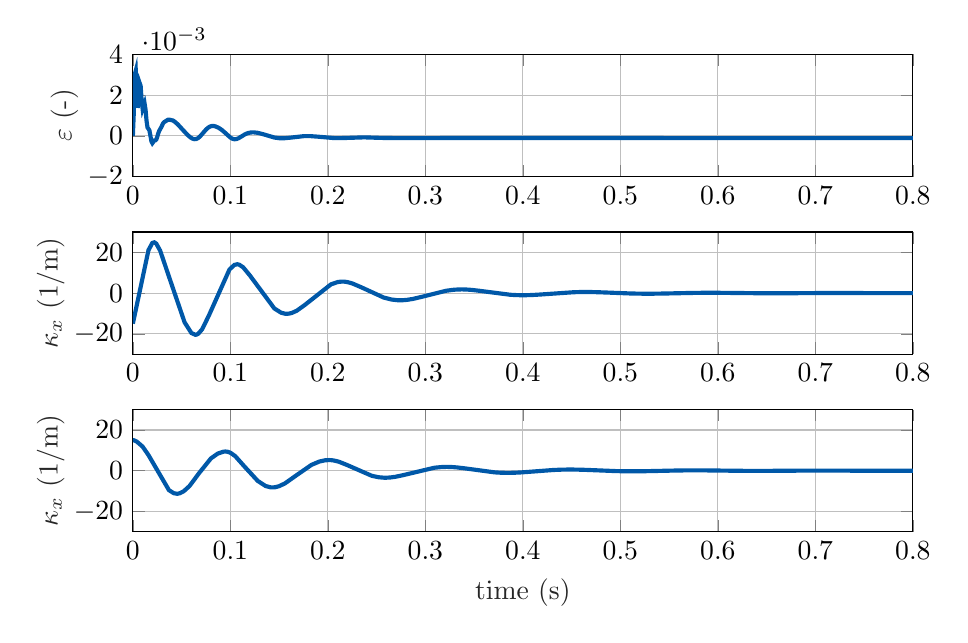
\begin{tikzpicture}

\begin{axis}[%
width=0.817\textwidth,
height=0.128\textwidth,
at={(0\textwidth,0.372\textwidth)},
scale only axis,
xmin=0,
xmax=0.8,
ymin=-0.002,
ymax=0.004,
ylabel style={font=\color{white!15!black}},
ylabel={$\varepsilon$ (-)},
axis background/.style={fill=white},
xmajorgrids,
ymajorgrids,
ylabel style={yshift=-3.5pt}
]
\addplot [color=mycolor1, line width=1.5pt, forget plot]
  table[row sep=crcr]{%
0	0\\
0.00100069999999997	0.00118280000000004\\
0.00200129999999998	0.00302690000000005\\
0.00300199999999995	0.00320659999999995\\
0.00400270000000003	0.00204000000000004\\
0.00500330000000004	0.00137810000000005\\
0.00600400000000001	0.00189989999999995\\
0.00700469999999997	0.00259039999999999\\
0.00800529999999999	0.00244929999999999\\
0.00900599999999996	0.00173400000000001\\
0.010007	0.00132149999999998\\
0.012008	0.0015965\\
0.013009	0.00129559999999995\\
0.014009	0.000752890000000006\\
0.01501	0.000412799999999991\\
0.016011	0.000345240000000024\\
0.017011	0.000263690000000039\\
0.018012	6.14200000004228e-06\\
0.0190129999999999	-0.000267059999999986\\
0.0200129999999999	-0.000355349999999977\\
0.022015	-0.000226130000000047\\
0.023015	-0.000218750000000045\\
0.024016	-0.000179099999999988\\
0.025017	-4.87319999999958e-05\\
0.026017	0.000119230000000026\\
0.027018	0.000247529999999996\\
0.029019	0.000416859999999963\\
0.031021	0.000616460000000041\\
0.032021	0.000675300000000045\\
0.0360240000000001	0.000792470000000045\\
0.038025	0.000790540000000006\\
0.041027	0.000757299999999961\\
0.043029	0.000692970000000015\\
0.046031	0.000568110000000011\\
0.0520350000000001	0.000254760000000021\\
0.056037	5.16750000000288e-05\\
0.059039	-7.46109999999467e-05\\
0.061041	-0.000132119999999958\\
0.063042	-0.00015993999999997\\
0.065043	-0.000150239999999968\\
0.067045	-0.000101770000000001\\
0.0690460000000001	-1.85299999999611e-05\\
0.072048	0.000146179999999996\\
0.0750500000000001	0.000311900000000032\\
0.077051	0.000399240000000023\\
0.079053	0.000458139999999996\\
0.081054	0.000486059999999955\\
0.083055	0.000485100000000016\\
0.085057	0.000460800000000039\\
0.088059	0.000394299999999959\\
0.0910610000000001	0.000299209999999994\\
0.094063	0.000176859999999945\\
0.10007	-8.26600000000122e-05\\
0.10207	-0.000138430000000023\\
0.10407	-0.000163899999999995\\
0.10607	-0.000156939999999994\\
0.10807	-0.000121860000000029\\
0.11107	-3.72770000000022e-05\\
0.11508	7.97289999999728e-05\\
0.11808	0.00013996000000005\\
0.12108	0.000169470000000005\\
0.12408	0.000173120000000027\\
0.12809	0.000150490000000003\\
0.13309	9.08080000000533e-05\\
0.1451	-7.99169999999849e-05\\
0.1501	-0.000113290000000044\\
0.1551	-0.000115599999999993\\
0.16111	-8.87210000000138e-05\\
0.17512	-1.33270000000074e-05\\
0.18212	-1.10450000000428e-05\\
0.19013	-3.9399000000051e-05\\
0.20714	-0.000110049999999973\\
0.21514	-0.000106530000000049\\
0.23716	-7.15239999999895e-05\\
0.25417	-9.7973000000029e-05\\
0.26918	-0.000108980000000036\\
0.36024	-0.000104609999999949\\
0.64943	-0.000108019999999986\\
0.80053	-0.000108019999999986\\
};
\end{axis}

\begin{axis}[%
width=0.817\textwidth,
height=0.128\textwidth,
at={(0\textwidth,0.186\textwidth)},
scale only axis,
xmin=0,
xmax=0.8,
ymin=-30,
ymax=30,
ylabel style={font=\color{white!15!black}},
ylabel={$\kappa_x$ (1/m)},
axis background/.style={fill=white},
xmajorgrids,
ymajorgrids,
ylabel style={yshift=-3.5pt}
]
\addplot [color=mycolor1, line width=1.5pt, forget plot]
  table[row sep=crcr]{%
0	-15\\
0.0160109999999989	21.093\\
0.0200129999999987	24.639\\
0.0220149999999997	24.921\\
0.0240159999999996	24.275\\
0.0280190000000005	20.825\\
0.0370249999999999	8.0954\\
0.0530350000000013	-14.326\\
0.0600400000000008	-19.584\\
0.0640430000000016	-20.462\\
0.0650429999999993	-20.405\\
0.0670450000000002	-19.956\\
0.0710470000000001	-17.783\\
0.0780519999999996	-10.912\\
0.0990660000000005	11.571\\
0.10407	13.835\\
0.10707	14.162\\
0.109069999999999	13.96\\
0.11308	12.693\\
0.120080000000002	8.6293\\
0.145099999999999	-7.5345\\
0.152100000000001	-9.6423\\
0.156099999999999	-10.114\\
0.158110000000001	-10.154\\
0.16011	-10.071\\
0.16311	-9.7278\\
0.168109999999999	-8.6433\\
0.176120000000001	-5.9078\\
0.203140000000001	4.2835\\
0.210139999999999	5.4359\\
0.21414	5.6507\\
0.215140000000002	5.6544\\
0.217140000000001	5.6043\\
0.22015	5.394\\
0.225149999999999	4.733\\
0.234159999999999	2.8837\\
0.257169999999999	-2.165\\
0.265180000000001	-3.1435\\
0.271180000000001	-3.478\\
0.274180000000001	-3.5186\\
0.275179999999999	-3.5142\\
0.277180000000001	-3.4797\\
0.281189999999999	-3.3144\\
0.287189999999999	-2.8582\\
0.296199999999999	-1.8413\\
0.321210000000001	1.1479\\
0.329219999999999	1.6489\\
0.334219999999998	1.7913\\
0.337219999999999	1.8136\\
0.339230000000001	1.8034\\
0.342230000000001	1.7526\\
0.34723	1.5834\\
0.355239999999998	1.144\\
0.387260000000001	-0.82525\\
0.394259999999999	-0.9984\\
0.39827	-1.0371\\
0.400269999999999	-1.0405\\
0.402270000000001	-1.0338\\
0.405270000000002	-1.0058\\
0.410270000000001	-0.91602\\
0.418279999999999	-0.684049999999999\\
0.452300000000001	0.438210000000002\\
0.458310000000001	0.51538\\
0.462309999999999	0.53706\\
0.464310000000001	0.53923\\
0.467310000000001	0.53219\\
0.471309999999999	0.504999999999999\\
0.477319999999999	0.431660000000001\\
0.48732	0.250540000000001\\
0.510339999999999	-0.179390000000001\\
0.518350000000002	-0.263059999999999\\
0.524349999999998	-0.29299\\
0.527349999999998	-0.2974\\
0.530349999999999	-0.295110000000001\\
0.53436	-0.28246\\
0.54036	-0.245730000000002\\
0.54937	-0.161860000000001\\
0.575379999999999	0.0987620000000007\\
0.583390000000001	0.141269999999999\\
0.589390000000002	0.155419999999999\\
0.593399999999999	0.156510000000001\\
0.5974	0.151420000000002\\
0.602399999999999	0.137350000000001\\
0.610410000000002	0.101030000000002\\
0.643429999999999	-0.0701439999999991\\
0.65043	-0.0844270000000016\\
0.655439999999999	-0.0876699999999992\\
0.660440000000001	-0.0854430000000015\\
0.666440000000001	-0.0764409999999991\\
0.67445	-0.0562310000000004\\
0.707470000000001	0.0381\\
0.715479999999999	0.0465310000000017\\
0.72148	0.0475339999999989\\
0.728490000000001	0.0435039999999987\\
0.737490000000001	0.0319460000000014\\
0.773520000000001	-0.0228089999999987\\
0.78152	-0.0262239999999991\\
0.789529999999999	-0.0253240000000012\\
0.799530000000001	-0.0192890000000006\\
0.800529999999998	-0.0184619999999995\\
};
\end{axis}

\begin{axis}[%
width=0.817\textwidth,
height=0.128\textwidth,
at={(0\textwidth,0\textwidth)},
scale only axis,
xmin=0,
xmax=0.8,
xlabel style={font=\color{white!15!black}},
xlabel={time (s)},
ymin=-30,
ymax=30,
ylabel style={font=\color{white!15!black}},
ylabel={$\kappa_x$ (1/m)},
axis background/.style={fill=white},
xmajorgrids,
ymajorgrids,
ylabel style={yshift=-3.5pt}
]
\addplot [color=mycolor1, line width=1.5pt, forget plot]
  table[row sep=crcr]{%
0	15\\
0.00100070000000052	14.95\\
0.00400269999999914	14.297\\
0.0100069999999999	11.814\\
0.0160110000000007	7.6573\\
0.0370249999999999	-9.5688\\
0.0420280000000002	-11.059\\
0.0450300000000006	-11.31\\
0.0460309999999993	-11.287\\
0.0480319999999992	-11.09\\
0.0520350000000001	-10.147\\
0.0580390000000008	-7.5546\\
0.0680449999999997	-1.1197\\
0.0800529999999995	6.0245\\
0.0870580000000007	8.3962\\
0.0930619999999998	9.3567\\
0.0950629999999997	9.4097\\
0.0970650000000006	9.3007\\
0.100070000000001	8.8078\\
0.10507	7.1137\\
0.11408	2.2559\\
0.12809	-5.0254\\
0.136089999999999	-7.5037\\
0.14109	-8.152\\
0.1431	-8.2116\\
0.1441	-8.1999\\
0.146100000000001	-8.0963\\
0.1501	-7.5893\\
0.1561	-6.1972\\
0.167109999999999	-2.4697\\
0.183120000000001	2.8362\\
0.191129999999999	4.4719\\
0.19713	5.1057\\
0.201129999999999	5.2204\\
0.203139999999999	5.1825\\
0.20614	5.008\\
0.21114	4.4251\\
0.219150000000001	2.9017\\
0.24516	-2.5238\\
0.25217	-3.2225\\
0.25717	-3.4262\\
0.259169999999999	-3.4404\\
0.26117	-3.4181\\
0.26418	-3.3202\\
0.26918	-3.0039\\
0.27718	-2.1924\\
0.30921	1.4497\\
0.31621	1.7737\\
0.320209999999999	1.8472\\
0.32221	1.8539\\
0.32422	1.8412\\
0.327220000000001	1.7872\\
0.33222	1.6127\\
0.34023	1.1607\\
0.37125	-0.826919999999999\\
0.37825	-1.0173\\
0.38326	-1.0668\\
0.384259999999999	-1.0684\\
0.387259999999999	-1.0571\\
0.391260000000001	-1.0076\\
0.397259999999999	-0.869759999999999\\
0.406269999999999	-0.56235\\
0.431290000000001	0.34328\\
0.43929	0.500870000000001\\
0.4453	0.555770000000001\\
0.4483	0.56293\\
0.4513	0.557230000000001\\
0.455299999999999	0.53106\\
0.461309999999999	0.457409999999999\\
0.47031	0.29191\\
0.495329999999999	-0.195040000000001\\
0.50334	-0.27852\\
0.50934	-0.30663\\
0.51234	-0.30972\\
0.51534	-0.30593\\
0.519349999999999	-0.290929999999999\\
0.52535	-0.25001\\
0.535360000000001	-0.14809\\
0.55837	0.0959800000000008\\
0.566380000000001	0.144310000000001\\
0.572380000000001	0.16215\\
0.57638	0.165240000000001\\
0.58039	0.1617\\
0.58539	0.14888\\
0.59239	0.11825\\
0.6044	0.0460480000000008\\
0.62041	-0.0462399999999992\\
0.62942	-0.0787340000000007\\
0.63542	-0.0896410000000003\\
0.64043	-0.092041\\
0.645429999999999	-0.0887689999999992\\
0.652430000000001	-0.0760450000000006\\
0.661440000000001	-0.0497449999999997\\
0.68746	0.0322759999999995\\
0.695460000000001	0.0455330000000007\\
0.70247	0.0501120000000004\\
0.70847	0.049004\\
0.715479999999999	0.0426590000000004\\
0.725479999999999	0.0269060000000003\\
0.7525	-0.0191949999999999\\
0.761509999999999	-0.0263190000000009\\
0.76951	-0.0276610000000002\\
0.777520000000001	-0.0247609999999998\\
0.78853	-0.0157760000000007\\
0.80053	-0.00321839999999973\\
};
\end{axis}
\end{tikzpicture}%
  \includegraphics*{./pdf/thesis-figure-4-14.pdf}
  \vspace{-3mm}
  \caption{State trajectories of one-link soft robot model with initial conditions $\q_0 = (0 , -15, 15)^\top$ and $\dq_0 = (0, 2500, 0)^\top$. The figure shows the elongation strain $\varepsilon$ and the curvatures $\kappa_x$, $\kappa_y$ in the $xz$-plane and $yz$-plane, respectively. Clearly the one-link soft robot oscillates about the set $\Omega_{\textrm{stab}}$. }
  \label{fig:C2:natural_states}
\end{figure}
%

%
\begin{figure}[!t]
  %\vspace{-3mm}
  \centering
  %% This file was created by matlab2tikz.
%
%The latest updates can be retrieved from
%  http://www.mathworks.com/matlabcentral/fileexchange/22022-matlab2tikz-matlab2tikz
%where you can also make suggestions and rate matlab2tikz.
%
\begin{tikzpicture}

\begin{axis}[%
width=0.216\textwidth,
height=0.199\textwidth,
at={(0\textwidth,0.253\textwidth)},
scale only axis,
axis on top,
xmin=0.5,
xmax=522.5,
tick align=outside,
y dir=reverse,
ymin=0.5,
ymax=458.5,
axis line style={draw=none},
ticks=none,
ylabel style={yshift=-7.5pt}
]
\addplot [forget plot] graphics [xmin=0.5, xmax=522.5, ymin=0.5, ymax=458.5] {./fig/fig_C2_natural_3D-1.png};
\end{axis}

\begin{axis}[%
width=0.216\textwidth,
height=0.199\textwidth,
at={(0.245\textwidth,0.253\textwidth)},
scale only axis,
axis on top,
xmin=0.5,
xmax=522.5,
tick align=outside,
y dir=reverse,
ymin=0.5,
ymax=458.5,
axis line style={draw=none},
ticks=none,
ylabel style={yshift=-7.5pt}
]
\addplot [forget plot] graphics [xmin=0.5, xmax=522.5, ymin=0.5, ymax=458.5] {./fig/fig_C2_natural_3D-2.png};
\end{axis}

\begin{axis}[%
width=0.216\textwidth,
height=0.199\textwidth,
at={(0.49\textwidth,0.253\textwidth)},
scale only axis,
axis on top,
xmin=0.5,
xmax=522.5,
tick align=outside,
y dir=reverse,
ymin=0.5,
ymax=458.5,
axis line style={draw=none},
ticks=none,
ylabel style={yshift=-7.5pt}
]
\addplot [forget plot] graphics [xmin=0.5, xmax=522.5, ymin=0.5, ymax=458.5] {./fig/fig_C2_natural_3D-3.png};
\end{axis}

\begin{axis}[%
width=0.216\textwidth,
height=0.199\textwidth,
at={(0.734\textwidth,0.253\textwidth)},
scale only axis,
axis on top,
xmin=0.5,
xmax=522.5,
tick align=outside,
y dir=reverse,
ymin=0.5,
ymax=458.5,
axis line style={draw=none},
ticks=none,
ylabel style={yshift=-7.5pt}
]
\addplot [forget plot] graphics [xmin=0.5, xmax=522.5, ymin=0.5, ymax=458.5] {./fig/fig_C2_natural_3D-4.png};
\end{axis}

\begin{axis}[%
width=0.216\textwidth,
height=0.199\textwidth,
at={(0\textwidth,0\textwidth)},
scale only axis,
axis on top,
xmin=0.5,
xmax=522.5,
tick align=outside,
y dir=reverse,
ymin=0.5,
ymax=458.5,
axis line style={draw=none},
ticks=none,
ylabel style={yshift=-7.5pt}
]
\addplot [forget plot] graphics [xmin=0.5, xmax=522.5, ymin=0.5, ymax=458.5] {./fig/fig_C2_natural_3D-5.png};
\end{axis}

\begin{axis}[%
width=0.216\textwidth,
height=0.199\textwidth,
at={(0.245\textwidth,0\textwidth)},
scale only axis,
axis on top,
xmin=0.5,
xmax=522.5,
tick align=outside,
y dir=reverse,
ymin=0.5,
ymax=458.5,
axis line style={draw=none},
ticks=none,
ylabel style={yshift=-7.5pt}
]
\addplot [forget plot] graphics [xmin=0.5, xmax=522.5, ymin=0.5, ymax=458.5] {./fig/fig_C2_natural_3D-6.png};
\end{axis}

\begin{axis}[%
width=0.216\textwidth,
height=0.199\textwidth,
at={(0.49\textwidth,0\textwidth)},
scale only axis,
axis on top,
xmin=0.5,
xmax=522.5,
tick align=outside,
y dir=reverse,
ymin=0.5,
ymax=458.5,
axis line style={draw=none},
ticks=none,
ylabel style={yshift=-7.5pt}
]
\addplot [forget plot] graphics [xmin=0.5, xmax=522.5, ymin=0.5, ymax=458.5] {./fig/fig_C2_natural_3D-7.png};
\end{axis}

\begin{axis}[%
width=0.216\textwidth,
height=0.199\textwidth,
at={(0.734\textwidth,0\textwidth)},
scale only axis,
axis on top,
xmin=0.5,
xmax=522.5,
tick align=outside,
y dir=reverse,
ymin=0.5,
ymax=458.5,
axis line style={draw=none},
ticks=none,
ylabel style={yshift=-7.5pt}
]
\addplot [forget plot] graphics [xmin=0.5, xmax=522.5, ymin=0.5, ymax=458.5] {./fig/fig_C2_natural_3D-8.png};
\end{axis}

\begin{axis}[%
width=0.969\textwidth,
height=0.51\textwidth,
at={(-0.01\textwidth,-0.029\textwidth)},
scale only axis,
xmin=0,
xmax=1,
ymin=0,
ymax=1,
axis line style={draw=none},
ticks=none,
axis x line*=bottom,
axis y line*=left,
ylabel style={yshift=-7.5pt}
]
\end{axis}
\end{tikzpicture}%
  \includegraphics*{./pdf/thesis-figure-4-15.pdf}
  \vspace{-3mm}
  \caption{Three-dimensional volumetric evolution of the one-link soft robot model with initial conditions $\q_0 = (0 , -15, 15)^\top$ and $\dq_0 = (0, 2500, 0)^\top$. Notice that the states of the one-link soft robot quickly converge to the the set of stable equilibria $\Omega_{\textrm{stab}}$. }
  \label{fig:C2:natural_3D}
\end{figure}
\clearpage
}

To illustrate the unforced dynamics and the existence of stable equilibria, time-domain simulations of the dynamical model with nonzero initial conditions:
%
\begin{align*}
\q_0 & = \left(0,\,-15,\,15\; \right)^\top, \\[0.35em] \dq_0 & = \left(0,\,2500,\,0 \right)^\top.
\end{align*}
%
Figure \ref{fig:C2:natural_states} shows the state trajectories of the soft robot; whereas Figure \ref{fig:C2:natural_3D} is provided to better illustrate the underlying dynamics and the trajectory of the end-effector.
%

Besides the existence of stable solutions, the numerical simulations perfectly illustrate the coupled dynamics between the elongation and bending of the soft robot. Due to the difference in mechanical stiffness for elongation and bending, we observe high-frequency and low-frequency oscillation for the elongation strain $\varepsilon(t)$, and we observe low-frequent oscillations for the curvatures $\kappa_x(t)$ and $\kappa_y(t)$. Interestingly, the low-frequency oscillations are passed from the curvature dynamics to elongation dynamics; conversely, the dynamics of the elongation barely affect the curvatures. After sufficient time passes, the trajectories indeed tend to the set of stable equilibria $\Omega_{\textrm{stab}}$.

\textbf{ Experimental comparison-- unforced, forced, and external loads}:
\noindent To validate the dynamic model, the solutions of the model are compared with measurements of the physical system in unforced,  forced, and tip-load conditions. As such, the model validation is separated into three parts: \textit{i)} unforced, \textit{ii)} forced conditions, and \textit{iii)} external tip-loads applied on the end-effector.

We start with the unforced scenario, \ie, no input is considered $u_i(t) \equiv 0$. For the unforced analysis, two experimental trails are performed for the unforced validation. First, the soft robot is deformed slightly and then released from rest, which corresponds to the initial conditions $\q_0 = \left(0.015,\,4.75,\,0 \right)^\top$ and $\dq_0 = \vec{0}_3$. Since the mechanical deformations are relatively small here, the presence of hyper-elastic and visco-elastic material behavior are less dominant. Secondly, the soft robot is moderately deformed such that the initial configuration (or shortly after) lies within the hyper-elastic and visco-elastic regime. In this scenario, the nonlinear and time-dependent material effects may not be neglected. These initial conditions correspond to $\q_0 = \left(0.046,\,11.25,\,0 \right)^\top$ and $\dq_0 = \vec{0}_3$. It is worth mentioning that the creep strains $\lambdaB$ are difficult to distinguish from the true strain, and thus the initial conditions for $\lambdaB(t_0)$ are determined empirically  using a set of dynamic measurements with different initial condition. The comparison between our model and the unforced dynamic measurements are shown in Figure \ref{fig:C2:compare_states}. 
% The associated code for the unforced validation simulations can be found under \texttt{./valid\_one\_link\_open.m}.


%
\begin{figure}[!t]
  %\vspace{-2mm}
  \centering
  %% This file was created by matlab2tikz.
%
\definecolor{mycolor1}{rgb}{0.00000,0.34510,0.65882}%
\definecolor{mycolor2}{rgb}{0.79216,0.11765,0.17255}%
\definecolor{mycolor3}{rgb}{0.20392,0.65490,0.24706}%
%
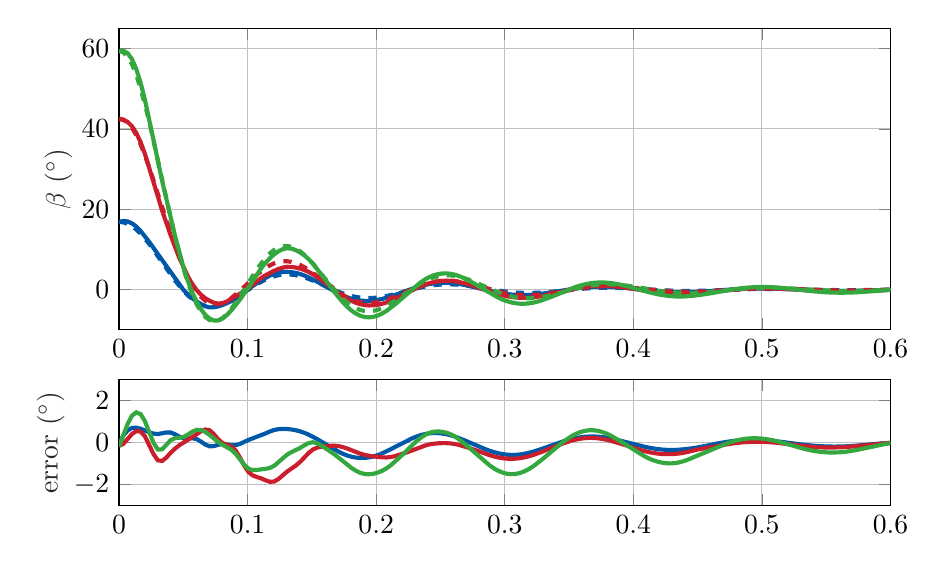
\begin{tikzpicture}

\begin{axis}[%
width=0.808\textwidth,
height=0.316\textwidth,
at={(0\textwidth,0.184\textwidth)},
scale only axis,
xmin=0,
xmax=0.6,
ymin=-10,
ymax=65,
ylabel style={font=\color{white!15!black}},
ylabel={$\beta$ ($^\circ$)},
axis background/.style={fill=white},
xmajorgrids,
ymajorgrids,
ylabel style={yshift=-3.5pt}
]
\addplot [color=mycolor1, dashed, line width=1.5pt, forget plot]
  table[row sep=crcr]{%
0	16.868\\
0.00335199999999958	16.745\\
0.00670390000000154	16.384\\
0.0100559999999987	15.79\\
0.0134079999999983	14.97\\
0.0167600000000014	13.945\\
0.0234640000000006	11.394\\
0.0335199999999993	6.8314\\
0.0435750000000006	2.2676\\
0.0502789999999997	-0.33305\\
0.0536309999999993	-1.4231\\
0.0569829999999989	-2.3479\\
0.0603349999999985	-3.0944\\
0.0636870000000016	-3.6543\\
0.0670390000000012	-4.0247\\
0.0703910000000008	-4.2083\\
0.0737430000000003	-4.2112\\
0.0770949999999999	-4.0455\\
0.0804469999999995	-3.7307\\
0.0837989999999991	-3.2873\\
0.0871509999999986	-2.7385\\
0.0938550000000014	-1.4243\\
0.10726	1.3805\\
0.113969999999998	2.5283\\
0.117319999999999	2.9815\\
0.12067	3.3404\\
0.124020000000002	3.5984\\
0.127369999999999	3.7524\\
0.13073	3.8024\\
0.134080000000001	3.7515\\
0.137429999999998	3.6056\\
0.140779999999999	3.3729\\
0.144130000000001	3.0638\\
0.147490000000001	2.6904\\
0.15419	1.8051\\
0.170950000000001	-0.55735\\
0.17765	-1.2954\\
0.181010000000001	-1.5817\\
0.184360000000002	-1.8053\\
0.187709999999999	-1.9631\\
0.19106	-2.0538\\
0.194410000000001	-2.0786\\
0.197769999999998	-2.0397\\
0.20112	-1.9422\\
0.204470000000001	-1.7919\\
0.207820000000002	-1.5962\\
0.21453	-1.102\\
0.234639999999999	0.561699999999998\\
0.23799	0.781110000000002\\
0.241340000000001	0.967829999999999\\
0.244689999999999	1.1182\\
0.24804	1.2298\\
0.2514	1.3014\\
0.254750000000001	1.3332\\
0.258099999999999	1.326\\
0.26145	1.282\\
0.264800000000001	1.2044\\
0.268160000000002	1.0971\\
0.271509999999999	0.964549999999999\\
0.278210000000001	0.64423\\
0.294969999999999	-0.228840000000002\\
0.301680000000001	-0.50535\\
0.305029999999999	-0.61336\\
0.30838	-0.698309999999999\\
0.311730000000001	-0.758929999999999\\
0.315080000000002	-0.794799999999999\\
0.318439999999999	-0.806080000000001\\
0.32179	-0.793690000000002\\
0.325140000000001	-0.7592\\
0.328489999999999	-0.704699999999999\\
0.33184	-0.63287\\
0.338550000000001	-0.449290000000001\\
0.35866	0.183789999999998\\
0.362010000000001	0.26942\\
0.365359999999999	0.34309\\
0.36872	0.403320000000001\\
0.372070000000001	0.449120000000001\\
0.375419999999998	0.479949999999999\\
0.378769999999999	0.49567\\
0.38212	0.49661\\
0.385470000000002	0.48348\\
0.388829999999999	0.457370000000001\\
0.39218	0.41966\\
0.395530000000001	0.372039999999998\\
0.402229999999999	0.254660000000001\\
0.422350000000002	-0.13081\\
0.425699999999999	-0.180910000000001\\
0.42905	-0.223320000000001\\
0.432400000000001	-0.257269999999998\\
0.435749999999999	-0.2822\\
0.439109999999999	-0.29785\\
0.442460000000001	-0.304259999999999\\
0.445810000000002	-0.3017\\
0.449159999999999	-0.29072\\
0.45251	-0.272040000000001\\
0.455870000000001	-0.246600000000001\\
0.459219999999998	-0.215450000000001\\
0.465920000000001	-0.140820000000001\\
0.482679999999998	0.0594210000000004\\
0.48939	0.1218\\
0.492740000000001	0.14592\\
0.496089999999999	0.16469\\
0.49944	0.177849999999999\\
0.502790000000001	0.185320000000001\\
0.506150000000002	0.187180000000001\\
0.509499999999999	0.18365\\
0.51285	0.17511\\
0.516200000000001	0.16206\\
0.519549999999999	0.14509\\
0.526260000000001	0.102180000000001\\
0.54637	-0.0440749999999994\\
0.549720000000001	-0.0636940000000017\\
0.553070000000002	-0.0805149999999983\\
0.556419999999999	-0.0942049999999988\\
0.55978	-0.10453\\
0.563130000000001	-0.11138\\
0.566479999999999	-0.114730000000002\\
0.56983	-0.114660000000001\\
0.573180000000001	-0.111339999999998\\
0.576540000000001	-0.105049999999999\\
0.579889999999999	-0.0961040000000004\\
0.58324	-0.084892\\
0.589939999999999	-0.0574340000000007\\
0.600000000000001	-0.0107409999999994\\
};
\addplot [color=mycolor1, line width=1.5pt, forget plot]
  table[row sep=crcr]{%
0	16.835677\\
0.00335199999999958	17.08401\\
0.00670390000000154	16.96115\\
0.0100559999999987	16.48681\\
0.0134079999999983	15.68434\\
0.0167600000000014	14.60635\\
0.0234640000000006	11.88233\\
0.0502789999999997	-0.123909999999999\\
0.0536309999999993	-1.22505\\
0.0569829999999989	-2.14127\\
0.0636870000000016	-3.60587\\
0.0670390000000012	-4.117172\\
0.0703910000000008	-4.38644\\
0.0737430000000003	-4.37765\\
0.0770949999999999	-4.15037\\
0.0804469999999995	-3.794186\\
0.0837989999999991	-3.369603\\
0.0871509999999986	-2.85922\\
0.0905030000000018	-2.23481\\
0.0972070000000009	-0.682357\\
0.103909999999999	0.91499\\
0.110610000000001	2.335\\
0.117319999999999	3.50976\\
0.12067	3.93963\\
0.124020000000002	4.23794\\
0.127369999999999	4.40479\\
0.13073	4.44793\\
0.134080000000001	4.37631\\
0.137429999999998	4.19383\\
0.140779999999999	3.9078\\
0.144130000000001	3.52886\\
0.147490000000001	3.06902\\
0.15419	1.96662\\
0.170950000000001	-0.997119999999999\\
0.174299999999999	-1.48891\\
0.17765	-1.91329\\
0.181010000000001	-2.25947\\
0.184360000000002	-2.52069\\
0.187709999999999	-2.69421\\
0.19106	-2.78114\\
0.194410000000001	-2.78397\\
0.197769999999998	-2.70261\\
0.20112	-2.54178\\
0.204470000000001	-2.30947\\
0.207820000000002	-2.01857\\
0.21453	-1.31844\\
0.231280000000002	0.60106\\
0.234639999999999	0.91722\\
0.23799	1.18767\\
0.241340000000001	1.40767\\
0.244689999999999	1.57359\\
0.24804	1.68273\\
0.2514	1.73467\\
0.254750000000001	1.73074\\
0.258099999999999	1.67251\\
0.26145	1.56393\\
0.264800000000001	1.41081\\
0.268160000000002	1.21999\\
0.27486	0.757010000000001\\
0.291620000000002	-0.521222999999999\\
0.29832	-0.92361\\
0.301680000000001	-1.07898\\
0.305029999999999	-1.1992\\
0.30838	-1.28158\\
0.311730000000001	-1.32483\\
0.315080000000002	-1.32943\\
0.318439999999999	-1.29709\\
0.32179	-1.23102\\
0.325140000000001	-1.13475\\
0.328489999999999	-1.01205\\
0.3352	-0.707100000000001\\
0.355309999999999	0.303149000000001\\
0.35866	0.434239999999999\\
0.362010000000001	0.544650000000001\\
0.365359999999999	0.632079999999998\\
0.36872	0.695039999999999\\
0.372070000000001	0.732949999999999\\
0.375419999999998	0.745619999999999\\
0.378769999999999	0.733229999999999\\
0.38212	0.696940000000001\\
0.385470000000002	0.639250000000001\\
0.388829999999999	0.563770000000002\\
0.395530000000001	0.3747522\\
0.40559	0.03538\\
0.412289999999999	-0.189534999999999\\
0.418990000000001	-0.382231000000001\\
0.422350000000002	-0.461600000000001\\
0.425699999999999	-0.526890000000002\\
0.42905	-0.57582\\
0.432400000000001	-0.606829999999999\\
0.435749999999999	-0.620280000000001\\
0.439109999999999	-0.617920000000002\\
0.442460000000001	-0.601880000000001\\
0.445810000000002	-0.572620000000001\\
0.449159999999999	-0.530000000000001\\
0.45251	-0.474409999999999\\
0.459219999999998	-0.334610000000001\\
0.47598	0.0465359999999997\\
0.482679999999998	0.168471\\
0.48603	0.216479\\
0.48939	0.254480000000001\\
0.492740000000001	0.281849999999999\\
0.496089999999999	0.298179999999999\\
0.49944	0.303380000000001\\
0.502790000000001	0.29776\\
0.506150000000002	0.282164000000002\\
0.509499999999999	0.257860000000001\\
0.51285	0.226277\\
0.516200000000001	0.188285\\
0.52291	0.0964060000000018\\
0.53631	-0.100956\\
0.543019999999999	-0.183433000000001\\
0.54637	-0.218154999999999\\
0.549720000000001	-0.247094000000001\\
0.553070000000002	-0.269435000000001\\
0.556419999999999	-0.284925000000001\\
0.55978	-0.29365\\
0.563130000000001	-0.295780000000001\\
0.566479999999999	-0.290959999999998\\
0.56983	-0.278839999999999\\
0.573180000000001	-0.259509999999999\\
0.576540000000001	-0.234649999999998\\
0.586590000000001	-0.146151\\
0.600000000000001	-0.0214819999999989\\
};
\addplot [color=mycolor2, dashed, line width=1.5pt, forget plot]
  table[row sep=crcr]{%
0	42.536\\
0.00335199999999958	42.282\\
0.00670389999999799	41.522\\
0.0100559999999987	40.242\\
0.0134079999999983	38.44\\
0.0167599999999979	36.168\\
0.023463999999997	30.502\\
0.0335200000000029	20.54\\
0.043574999999997	10.857\\
0.0502790000000033	5.412\\
0.0536310000000029	3.1194\\
0.0569830000000024	1.1481\\
0.060335000000002	-0.487009999999998\\
0.0636870000000016	-1.7789\\
0.0670390000000012	-2.7282\\
0.0703910000000008	-3.3431\\
0.0737430000000003	-3.639\\
0.0770949999999999	-3.6325\\
0.0804469999999995	-3.352\\
0.0837989999999991	-2.8415\\
0.0871509999999986	-2.1406\\
0.0938549999999978	-0.335940000000001\\
0.107259999999997	3.7242\\
0.113970000000002	5.3975\\
0.117319999999999	6.0468\\
0.120669999999997	6.5469\\
0.124020000000002	6.8862\\
0.127369999999999	7.059\\
0.13073	7.0669\\
0.134079999999997	6.9137\\
0.137430000000002	6.6076\\
0.140779999999999	6.1622\\
0.144129999999997	5.5948\\
0.150840000000002	4.176\\
0.174300000000002	-1.3647\\
0.17765	-1.9507\\
0.181010000000001	-2.4386\\
0.184359999999998	-2.8197\\
0.187710000000003	-3.0891\\
0.19106	-3.2449\\
0.194409999999998	-3.289\\
0.197769999999998	-3.2264\\
0.201120000000003	-3.0652\\
0.204470000000001	-2.8158\\
0.207819999999998	-2.4909\\
0.214530000000003	-1.6723\\
0.234639999999999	1.0494\\
0.237990000000003	1.402\\
0.241340000000001	1.6994\\
0.244689999999999	1.9358\\
0.248040000000003	2.1075\\
0.251399999999997	2.2128\\
0.254750000000001	2.252\\
0.258099999999999	2.2273\\
0.261450000000004	2.1423\\
0.264800000000001	2.0024\\
0.268160000000002	1.8144\\
0.271509999999999	1.5859\\
0.278210000000001	1.0417\\
0.294969999999999	-0.412089999999999\\
0.301679999999998	-0.86383\\
0.305030000000002	-1.0381\\
0.30838	-1.1733\\
0.311729999999997	-1.2676\\
0.315080000000002	-1.3204\\
0.318440000000002	-1.3323\\
0.32179	-1.305\\
0.325139999999998	-1.2412\\
0.328490000000002	-1.1448\\
0.33184	-1.0203\\
0.338549999999998	-0.707819999999998\\
0.35866	0.340719999999997\\
0.362009999999998	0.479120000000002\\
0.365360000000003	0.597029999999997\\
0.368720000000003	0.692140000000002\\
0.372070000000001	0.76294\\
0.375419999999998	0.808669999999999\\
0.378770000000003	0.829360000000001\\
0.38212	0.82564\\
0.385469999999998	0.798839999999998\\
0.388829999999999	0.750839999999997\\
0.392180000000003	0.684170000000002\\
0.395530000000001	0.601649999999999\\
0.402230000000003	0.401820000000001\\
0.418990000000001	-0.14405\\
0.425699999999999	-0.317210000000003\\
0.429049999999997	-0.384929999999997\\
0.432400000000001	-0.438249999999996\\
0.435749999999999	-0.476390000000002\\
0.439109999999999	-0.499079999999999\\
0.442459999999997	-0.506410000000002\\
0.445810000000002	-0.498950000000001\\
0.449159999999999	-0.47766\\
0.452509999999997	-0.443860000000001\\
0.455869999999997	-0.399140000000003\\
0.462569999999999	-0.284579999999998\\
0.482680000000002	0.112310000000001\\
0.48603	0.166229999999999\\
0.48939	0.212710000000001\\
0.492739999999998	0.250810000000001\\
0.496090000000002	0.279910000000001\\
0.49944	0.299630000000001\\
0.502789999999997	0.309890000000003\\
0.506149999999998	0.310859999999998\\
0.509500000000003	0.30301\\
0.51285	0.286999999999999\\
0.516199999999998	0.263689999999997\\
0.519550000000002	0.234119999999997\\
0.526260000000001	0.160879999999999\\
0.546370000000003	-0.0808520000000001\\
0.549720000000001	-0.112430000000003\\
0.553069999999998	-0.139220000000002\\
0.556420000000003	-0.160699999999999\\
0.559780000000003	-0.176549999999999\\
0.563130000000001	-0.186590000000002\\
0.566479999999999	-0.190829999999998\\
0.569830000000003	-0.189459999999997\\
0.573180000000001	-0.182780000000001\\
0.576540000000001	-0.17127\\
0.579889999999999	-0.15549\\
0.583240000000004	-0.136110000000002\\
0.589939999999999	-0.0895119999999991\\
0.600000000000001	-0.011845000000001\\
};
\addplot [color=mycolor2, line width=1.5pt, forget plot]
  table[row sep=crcr]{%
0	42.38149\\
0.00335199999999958	42.222217\\
0.00670389999999799	41.69166\\
0.0100559999999987	40.65025\\
0.0134079999999983	38.98657\\
0.0167599999999979	36.69417\\
0.0201119999999975	33.80024\\
0.0268159999999966	26.73915\\
0.0335200000000029	19.66599\\
0.0402229999999975	13.45309\\
0.0469269999999966	7.87586\\
0.0536310000000029	3.25341\\
0.0569830000000024	1.40726\\
0.060335000000002	-0.0902999999999992\\
0.0636870000000016	-1.24237\\
0.0670390000000012	-2.1044\\
0.0703910000000008	-2.75345\\
0.0737430000000003	-3.23569\\
0.0770949999999999	-3.46911\\
0.0804469999999995	-3.372993\\
0.0837989999999991	-2.94807\\
0.0972069999999974	-0.395600000000002\\
0.100560000000002	0.331299999999999\\
0.110610000000001	2.9104\\
0.113970000000002	3.6018\\
0.120669999999997	4.6932\\
0.124020000000002	5.1535\\
0.127369999999999	5.5033\\
0.13073	5.6872\\
0.134079999999997	5.6782\\
0.137430000000002	5.5108\\
0.140779999999999	5.23649\\
0.144129999999997	4.88484\\
0.147489999999998	4.43095\\
0.150840000000002	3.84732\\
0.157539999999997	2.33684\\
0.170949999999998	-0.86054\\
0.17765	-2.23809\\
0.181010000000001	-2.8069\\
0.184359999999998	-3.27132\\
0.187710000000003	-3.61586\\
0.19106	-3.83113\\
0.194409999999998	-3.91704\\
0.197769999999998	-3.88335\\
0.201120000000003	-3.746\\
0.204470000000001	-3.51687\\
0.207819999999998	-3.19829\\
0.211170000000003	-2.79457\\
0.217880000000001	-1.7955\\
0.231279999999998	0.353099999999998\\
0.237990000000003	1.25886\\
0.241340000000001	1.611332\\
0.244689999999999	1.882304\\
0.248040000000003	2.07225\\
0.251399999999997	2.18581\\
0.254750000000001	2.224886\\
0.258099999999999	2.186905\\
0.261450000000004	2.071465\\
0.264800000000001	1.88453\\
0.268160000000002	1.63768\\
0.274859999999997	1.01637\\
0.28492	-0.0867000000000004\\
0.291620000000002	-0.80386\\
0.298319999999997	-1.39718\\
0.301679999999998	-1.6287\\
0.305030000000002	-1.81002\\
0.30838	-1.93746\\
0.311729999999997	-2.00987\\
0.315080000000002	-2.02718\\
0.318440000000002	-1.99044\\
0.32179	-1.90267\\
0.325139999999998	-1.76848\\
0.328490000000002	-1.59428\\
0.3352	-1.15612\\
0.355310000000003	0.328949999999999\\
0.35866	0.523699999999998\\
0.362009999999998	0.688519999999997\\
0.365360000000003	0.819670000000002\\
0.368720000000003	0.914059999999999\\
0.372070000000001	0.970179999999999\\
0.375419999999998	0.988129999999998\\
0.378770000000003	0.969700000000003\\
0.38212	0.917717000000003\\
0.385469999999998	0.835248999999997\\
0.388829999999999	0.725577000000001\\
0.392180000000003	0.593209999999999\\
0.398879999999998	0.279899999999998\\
0.412289999999999	-0.390295000000002\\
0.418990000000001	-0.667409999999997\\
0.422350000000002	-0.778849999999998\\
0.425699999999999	-0.868859999999998\\
0.429049999999997	-0.935580000000002\\
0.432400000000001	-0.977899999999998\\
0.435749999999999	-0.994500000000002\\
0.439109999999999	-0.98433\\
0.442459999999997	-0.947589999999998\\
0.445810000000002	-0.88973\\
0.452509999999997	-0.744720000000001\\
0.459220000000002	-0.580199999999998\\
0.465919999999997	-0.379860000000001\\
0.47598	-0.0658239999999992\\
0.482680000000002	0.111078599999999\\
0.48603	0.182969999999997\\
0.48939	0.242019999999997\\
0.492739999999998	0.287495999999997\\
0.496090000000002	0.318967000000001\\
0.49944	0.33634\\
0.502789999999997	0.339979\\
0.506149999999998	0.329819999999998\\
0.509500000000003	0.305956700000003\\
0.51285	0.269086999999999\\
0.516199999999998	0.221479000000002\\
0.522910000000003	0.106288999999997\\
0.543019999999999	-0.264116999999999\\
0.546370000000003	-0.309241999999998\\
0.549720000000001	-0.346110000000003\\
0.553069999999998	-0.374450000000003\\
0.556420000000003	-0.393749999999997\\
0.559780000000003	-0.403669999999998\\
0.563130000000001	-0.404229999999998\\
0.566479999999999	-0.395890000000001\\
0.569830000000003	-0.379510000000003\\
0.573180000000001	-0.356029999999997\\
0.576540000000001	-0.326039999999999\\
0.579889999999999	-0.290089999999999\\
0.586590000000001	-0.204444000000002\\
0.600000000000001	-0.023690000000002\\
};
\addplot [color=mycolor3, dashed, line width=1.5pt, forget plot]
  table[row sep=crcr]{%
0	59.404\\
0.00335199999999958	59.027\\
0.00670389999999799	57.906\\
0.0100559999999987	56.032\\
0.0134079999999983	53.41\\
0.0167599999999979	50.113\\
0.023463999999997	41.896\\
0.0335200000000029	27.3714\\
0.043574999999997	13.1246\\
0.0502790000000033	5.07895\\
0.0536310000000029	1.6963\\
0.0569830000000024	-1.1998\\
0.060335000000002	-3.58141\\
0.0636870000000016	-5.4332\\
0.0670390000000012	-6.7529\\
0.0703910000000008	-7.5514\\
0.0737430000000003	-7.8502\\
0.0770949999999999	-7.678\\
0.0804469999999995	-7.0827\\
0.0837989999999991	-6.1288\\
0.0871509999999986	-4.8791\\
0.0938549999999978	-1.76024\\
0.107259999999997	5.1047\\
0.113970000000002	7.9258\\
0.117319999999999	9.0283\\
0.120669999999997	9.8873\\
0.124020000000002	10.4846\\
0.127369999999999	10.8114\\
0.13073	10.8693\\
0.134079999999997	10.6652\\
0.137430000000002	10.2132\\
0.140779999999999	9.5351\\
0.144129999999997	8.6586\\
0.150840000000002	6.4422\\
0.160890000000002	2.51421\\
0.1676	-0.0701350000000005\\
0.174300000000002	-2.31624\\
0.17765	-3.2461\\
0.181010000000001	-4.0203\\
0.184359999999998	-4.625\\
0.187710000000003	-5.0522\\
0.19106	-5.2987\\
0.194409999999998	-5.3676\\
0.197769999999998	-5.2661\\
0.201120000000003	-5.0074\\
0.204470000000001	-4.6077\\
0.207819999999998	-4.0871\\
0.214530000000003	-2.7743\\
0.234639999999999	1.6111\\
0.237990000000003	2.18311\\
0.241340000000001	2.66723\\
0.244689999999999	3.054\\
0.248040000000003	3.3373\\
0.251399999999997	3.5142\\
0.254750000000001	3.5852\\
0.258099999999999	3.5533\\
0.261450000000004	3.4243\\
0.264800000000001	3.2068\\
0.268160000000002	2.9115\\
0.271509999999999	2.55045\\
0.278210000000001	1.68593\\
0.294969999999999	-0.640929999999997\\
0.301679999999998	-1.36918\\
0.305030000000002	-1.65146\\
0.30838	-1.87161\\
0.311729999999997	-2.02653\\
0.315080000000002	-2.1152\\
0.318440000000002	-2.13838\\
0.32179	-2.09869\\
0.325139999999998	-2.0004\\
0.328490000000002	-1.8495\\
0.33184	-1.65317\\
0.338549999999998	-1.15711\\
0.35866	0.524509999999999\\
0.362009999999998	0.748539999999998\\
0.365360000000003	0.94012\\
0.368720000000003	1.09546\\
0.372070000000001	1.21206\\
0.375419999999998	1.28862\\
0.378770000000003	1.32503\\
0.38212	1.32225\\
0.385469999999998	1.28232\\
0.388829999999999	1.20821\\
0.392180000000003	1.10383\\
0.395530000000001	0.973689999999998\\
0.402230000000003	0.656480000000002\\
0.418990000000001	-0.218150999999999\\
0.425699999999999	-0.49812\\
0.429049999999997	-0.608249999999998\\
0.432400000000001	-0.695520000000002\\
0.435749999999999	-0.758589999999998\\
0.439109999999999	-0.796930000000003\\
0.442459999999997	-0.810670000000002\\
0.445810000000002	-0.800649999999997\\
0.449159999999999	-0.768380000000001\\
0.452509999999997	-0.715899999999998\\
0.455869999999997	-0.645740000000004\\
0.459220000000002	-0.560830000000003\\
0.465919999999997	-0.359639999999999\\
0.479329999999997	0.0746660000000006\\
0.48603	0.258999000000003\\
0.48939	0.334510000000002\\
0.492739999999998	0.396729999999998\\
0.496090000000002	0.444600000000001\\
0.49944	0.47748\\
0.502789999999997	0.49521\\
0.506149999999998	0.498040000000003\\
0.509500000000003	0.486660000000001\\
0.51285	0.462110000000003\\
0.516199999999998	0.425750000000001\\
0.519550000000002	0.37921\\
0.526260000000001	0.263060000000003\\
0.546370000000003	-0.124927\\
0.549720000000001	-0.176124000000002\\
0.553069999999998	-0.219735\\
0.556420000000003	-0.254905000000001\\
0.559780000000003	-0.281080000000003\\
0.563130000000001	-0.297969999999999\\
0.566479999999999	-0.30556\\
0.569830000000003	-0.304119999999998\\
0.573180000000001	-0.294119999999999\\
0.576540000000001	-0.276319999999998\\
0.579889999999999	-0.251593999999997\\
0.583240000000004	-0.221001999999999\\
0.589939999999999	-0.146946\\
0.600000000000001	-0.0225859999999969\\
};
\addplot [color=mycolor3, line width=1.5pt, forget plot]
  table[row sep=crcr]{%
0	59.20908625\\
0.00335199999999958	59.3909795\\
0.00670389999999799	58.7970975\\
0.0100559999999987	57.3112625\\
0.0134079999999983	54.849495\\
0.0167599999999979	51.4658575\\
0.0201119999999975	47.260615\\
0.0268159999999966	37.207375\\
0.0335200000000029	27.0502525\\
0.043574999999997	13.33534\\
0.0502790000000033	5.35124\\
0.0536310000000029	2.0778725\\
0.0569830000000024	-0.6823525\\
0.060335000000002	-2.9737125\\
0.0636870000000016	-4.8361325\\
0.0670390000000012	-6.24469\\
0.0703910000000008	-7.184425\\
0.0737430000000003	-7.6549525\\
0.0770949999999999	-7.6456975\\
0.0804469999999995	-7.1830505\\
0.0837989999999991	-6.33824875\\
0.0871509999999986	-5.21137\\
0.0938549999999978	-2.5357775\\
0.100560000000002	0.496741\\
0.110610000000001	5.331575\\
0.113970000000002	6.6766375\\
0.117319999999999	7.823225\\
0.120669999999997	8.7826375\\
0.124020000000002	9.551325\\
0.127369999999999	10.0711875\\
0.13073	10.2965125\\
0.134079999999997	10.2107125\\
0.137430000000002	9.8516875\\
0.140779999999999	9.278015\\
0.144129999999997	8.529965\\
0.147489999999998	7.594625\\
0.150840000000002	6.459195\\
0.157539999999997	3.706545\\
0.1676	-0.631464999999999\\
0.174300000000002	-3.2056025\\
0.17765	-4.3058525\\
0.181010000000001	-5.2358125\\
0.184359999999998	-5.9708575\\
0.187710000000003	-6.4928475\\
0.19106	-6.794105\\
0.194409999999998	-6.8773525\\
0.197769999999998	-6.7516875\\
0.201120000000003	-6.437675\\
0.204470000000001	-5.9557325\\
0.207819999999998	-5.3224525\\
0.214530000000003	-3.69141\\
0.234639999999999	1.83992\\
0.237990000000003	2.54817\\
0.241340000000001	3.128962\\
0.244689999999999	3.5697415\\
0.248040000000003	3.8682125\\
0.251399999999997	4.0287975\\
0.254750000000001	4.055011\\
0.258099999999999	3.9460425\\
0.261450000000004	3.7058775\\
0.264800000000001	3.3469425\\
0.268160000000002	2.8883925\\
0.274859999999997	1.759675\\
0.294969999999999	-1.9836175\\
0.298319999999997	-2.4576275\\
0.301679999999998	-2.8510875\\
0.305030000000002	-3.15568\\
0.30838	-3.3648575\\
0.311729999999997	-3.476175\\
0.315080000000002	-3.4902675\\
0.318440000000002	-3.4102825\\
0.32179	-3.2430225\\
0.325139999999998	-2.9971175\\
0.328490000000002	-2.6831675\\
0.3352	-1.90333\\
0.355310000000003	0.685859000000001\\
0.35866	1.0205525\\
0.362009999999998	1.3019775\\
0.365360000000003	1.5239975\\
0.368720000000003	1.68203\\
0.372070000000001	1.7740875\\
0.375419999999998	1.8001675\\
0.378770000000003	1.76232\\
0.38212	1.6647395\\
0.385469999999998	1.5134415\\
0.388829999999999	1.315947\\
0.395530000000001	0.818360249999998\\
0.405589999999997	-0.0653424999999999\\
0.412289999999999	-0.640605000000001\\
0.418990000000001	-1.1266735\\
0.422350000000002	-1.3231475\\
0.425699999999999	-1.482245\\
0.429049999999997	-1.599525\\
0.432400000000001	-1.67212\\
0.435749999999999	-1.6993\\
0.439109999999999	-1.6822675\\
0.442459999999997	-1.623875\\
0.445810000000002	-1.53008\\
0.449159999999999	-1.40915\\
0.455869999999997	-1.1147525\\
0.462569999999999	-0.7605425\\
0.47598	-0.00339625000000154\\
0.482680000000002	0.306812100000002\\
0.48603	0.430376500000001\\
0.48939	0.529670000000003\\
0.492739999999998	0.603328500000003\\
0.496090000000002	0.650519500000001\\
0.49944	0.671102500000003\\
0.502789999999997	0.665849000000001\\
0.506149999999998	0.635730000000002\\
0.509500000000003	0.582369200000002\\
0.51285	0.50815575\\
0.516199999999998	0.416320249999998\\
0.522910000000003	0.195574000000001\\
0.53631	-0.284416999999998\\
0.543019999999999	-0.487884999999999\\
0.546370000000003	-0.570917000000001\\
0.549720000000001	-0.639054000000002\\
0.553069999999998	-0.691115000000003\\
0.556420000000003	-0.726354999999998\\
0.559780000000003	-0.744599999999998\\
0.563130000000001	-0.746110000000002\\
0.566479999999999	-0.730907500000001\\
0.569830000000003	-0.699395000000003\\
0.573180000000001	-0.652582500000001\\
0.576540000000001	-0.593089999999997\\
0.583240000000004	-0.4487345\\
0.600000000000001	-0.0478572499999999\\
};
\end{axis}

\begin{axis}[%
width=0.808\textwidth,
height=0.132\textwidth,
at={(0\textwidth,0\textwidth)},
scale only axis,
xmin=0,
xmax=0.6,
ymin=-3,
ymax=3,
ylabel style={font=\color{white!15!black}},
ylabel={error ($^\circ$)},
axis background/.style={fill=white},
xmajorgrids,
ymajorgrids,
ylabel style={yshift=-3.5pt}
]
\addplot [color=mycolor1, line width=1.5pt, forget plot]
  table[row sep=crcr]{%
0	-0.032323\\
0.00335200000000002	0.33901\\
0.00670389999999998	0.57715\\
0.010056	0.69681\\
0.013408	0.71434\\
0.01676	0.66135\\
0.023464	0.48833\\
0.026816	0.42674\\
0.030168	0.40919\\
0.03352	0.44229\\
0.036872	0.48374\\
0.040223	0.47922\\
0.043575	0.39732\\
0.0469270000000001	0.28669\\
0.050279	0.20914\\
0.053631	0.19805\\
0.056983	0.20663\\
0.060335	0.16879\\
0.063687	0.04843\\
0.067039	-0.092472\\
0.070391	-0.17814\\
0.073743	-0.16645\\
0.077095	-0.10487\\
0.080447	-0.063486\\
0.083799	-0.082303\\
0.087151	-0.12072\\
0.090503	-0.12581\\
0.093855	-0.067574\\
0.10056	0.12356\\
0.11397	0.43723\\
0.11732	0.52826\\
0.12067	0.59923\\
0.12402	0.63954\\
0.12737	0.65239\\
0.13073	0.64553\\
0.13408	0.62481\\
0.13743	0.58823\\
0.14078	0.5349\\
0.14413	0.46506\\
0.14749	0.37862\\
0.15419	0.16152\\
0.17095	-0.43977\\
0.1743	-0.53737\\
0.17765	-0.61789\\
0.18101	-0.67777\\
0.18436	-0.71539\\
0.18771	-0.73111\\
0.19106	-0.72734\\
0.19441	-0.70537\\
0.19777	-0.66291\\
0.20112	-0.59958\\
0.20447	-0.51757\\
0.21117	-0.32053\\
0.22793	0.20113\\
0.23128	0.28666\\
0.23464	0.35552\\
0.23799	0.40656\\
0.24134	0.43984\\
0.24469	0.45539\\
0.24804	0.45293\\
0.2514	0.43327\\
0.25475	0.39754\\
0.2581	0.34651\\
0.26145	0.28193\\
0.26816	0.12289\\
0.28492	-0.31453\\
0.28827	-0.38975\\
0.29162	-0.45473\\
0.29497	-0.50759\\
0.29832	-0.54735\\
0.30168	-0.57363\\
0.30503	-0.58584\\
0.30838	-0.58327\\
0.31173	-0.5659\\
0.31508	-0.53463\\
0.31844	-0.49101\\
0.32179	-0.43733\\
0.32849	-0.30735\\
0.34525	0.053795\\
0.35196	0.16971\\
0.35531	0.21504\\
0.35866	0.25045\\
0.36201	0.27523\\
0.36536	0.28899\\
0.36872	0.29172\\
0.37207	0.28383\\
0.37542	0.26567\\
0.37877	0.23756\\
0.38212	0.20033\\
0.38883	0.1064\\
0.40894	-0.20102\\
0.41229	-0.2431\\
0.41564	-0.27887\\
0.41899	-0.30813\\
0.42235	-0.33079\\
0.4257	-0.34598\\
0.42905	-0.3525\\
0.4324	-0.34956\\
0.43575	-0.33808\\
0.43911	-0.32007\\
0.44246	-0.29762\\
0.44581	-0.27092\\
0.44916	-0.23928\\
0.45587	-0.16157\\
0.46592	-0.03757\\
0.47263	0.033613\\
0.47598	0.063567\\
0.47933	0.088888\\
0.48268	0.10905\\
0.48603	0.12371\\
0.48939	0.13268\\
0.49274	0.13593\\
0.49609	0.13349\\
0.49944	0.12553\\
0.50279	0.11244\\
0.50615	0.094984\\
0.51285	0.051167\\
0.51955	-0.00045187999999996\\
0.52961	-0.08325\\
0.53631	-0.12772\\
0.53966	-0.14575\\
0.54302	-0.16134\\
0.54637	-0.17408\\
0.54972	-0.1834\\
0.55307	-0.18892\\
0.55642	-0.19072\\
0.55978	-0.18912\\
0.56313	-0.1844\\
0.56648	-0.17623\\
0.56983	-0.16418\\
0.57318	-0.14817\\
0.58994	-0.057462\\
0.6	-0.010741\\
};
\addplot [color=mycolor2, line width=1.5pt, forget plot]
  table[row sep=crcr]{%
0	-0.15451\\
0.00335200000000002	-0.0597829999999999\\
0.0100560000000001	0.40825\\
0.0134080000000001	0.54657\\
0.0167600000000001	0.52617\\
0.0201119999999999	0.30624\\
0.026816	-0.54585\\
0.030168	-0.84419\\
0.03352	-0.87401\\
0.036872	-0.71092\\
0.0402229999999999	-0.48091\\
0.0435749999999999	-0.28591\\
0.0469269999999999	-0.12624\\
0.053631	0.13401\\
0.060335	0.39671\\
0.063687	0.53653\\
0.0670390000000001	0.6238\\
0.0703910000000001	0.58965\\
0.0737430000000001	0.40331\\
0.0770949999999999	0.16339\\
0.0804469999999999	-0.020993\\
0.087151	-0.18137\\
0.090503	-0.35827\\
0.093855	-0.69107\\
0.097207	-1.0783\\
0.10056	-1.3928\\
0.10391	-1.5603\\
0.10726	-1.6395\\
0.11061	-1.7054\\
0.11397	-1.7957\\
0.11732	-1.8654\\
0.12067	-1.8537\\
0.12402	-1.7327\\
0.13073	-1.3797\\
0.13743	-1.0968\\
0.14078	-0.92571\\
0.14749	-0.49435\\
0.15084	-0.32868\\
0.15419	-0.23688\\
0.15754	-0.19466\\
0.16089	-0.17258\\
0.16425	-0.15447\\
0.1676	-0.14873\\
0.17095	-0.16811\\
0.1743	-0.21765\\
0.17765	-0.28739\\
0.18771	-0.52676\\
0.19106	-0.58623\\
0.19441	-0.62804\\
0.19777	-0.65695\\
0.20112	-0.6808\\
0.20447	-0.70107\\
0.20782	-0.70739\\
0.21117	-0.68987\\
0.21453	-0.64656\\
0.22123	-0.51825\\
0.22793	-0.37474\\
0.23799	-0.14314\\
0.24134	-0.088068\\
0.24469	-0.053496\\
0.24804	-0.03525\\
0.2514	-0.0269900000000001\\
0.25475	-0.0271140000000001\\
0.2581	-0.040395\\
0.26145	-0.070835\\
0.2648	-0.11787\\
0.27151	-0.2415\\
0.27821	-0.37962\\
0.28827	-0.59824\\
0.29162	-0.65934\\
0.29497	-0.7082\\
0.29832	-0.74348\\
0.30168	-0.76487\\
0.30503	-0.77192\\
0.30838	-0.76416\\
0.31173	-0.74227\\
0.31508	-0.70678\\
0.31844	-0.65814\\
0.32179	-0.59767\\
0.32849	-0.44948\\
0.34525	-0.039194\\
0.35196	0.093342\\
0.35531	0.14413\\
0.35866	0.18298\\
0.36201	0.2094\\
0.36536	0.22264\\
0.36872	0.22192\\
0.37207	0.20724\\
0.37542	0.17946\\
0.37877	0.14034\\
0.38212	0.092077\\
0.38883	-0.025263\\
0.40559	-0.35361\\
0.40894	-0.40888\\
0.41229	-0.45621\\
0.41564	-0.49453\\
0.41899	-0.52336\\
0.42235	-0.5425\\
0.4257	-0.55165\\
0.42905	-0.55065\\
0.4324	-0.53965\\
0.43575	-0.51811\\
0.43911	-0.48525\\
0.44246	-0.44118\\
0.44916	-0.34167\\
0.45251	-0.30086\\
0.46257	-0.19941\\
0.47263	-0.085874\\
0.47598	-0.0530060000000001\\
0.47933	-0.0245839999999999\\
0.48268	-0.00123139999999999\\
0.48603	0.01674\\
0.48939	0.0293099999999999\\
0.49274	0.036686\\
0.49609	0.0390569999999999\\
0.49944	0.03671\\
0.50279	0.030089\\
0.50615	0.0189600000000001\\
0.5095	0.00294670000000008\\
0.51285	-0.0179130000000001\\
0.53631	-0.1865\\
0.53966	-0.20495\\
0.54302	-0.21894\\
0.54637	-0.22839\\
0.54972	-0.23368\\
0.55307	-0.23523\\
0.55642	-0.23305\\
0.55978	-0.22712\\
0.56313	-0.21764\\
0.56648	-0.20506\\
0.57318	-0.17325\\
0.57989	-0.1346\\
0.59665	-0.028394\\
0.6	-0.0118450000000001\\
};
\addplot [color=mycolor3, line width=1.5pt, forget plot]
  table[row sep=crcr]{%
0	-0.19491375\\
0.00670389999999998	0.8910975\\
0.0100560000000001	1.2792625\\
0.0134080000000001	1.439495\\
0.0167600000000001	1.3528575\\
0.0201119999999999	1.023615\\
0.026816	-0.0124249999999999\\
0.030168	-0.3327025\\
0.03352	-0.3211475\\
0.0402229999999999	0.118115\\
0.0435749999999999	0.21074\\
0.0469269999999999	0.2321225\\
0.050279	0.27229\\
0.053631	0.3815725\\
0.056983	0.5174475\\
0.060335	0.6076975\\
0.063687	0.5970675\\
0.0670390000000001	0.50821\\
0.0703910000000001	0.366975\\
0.0770949999999999	0.0323025000000001\\
0.0804469999999999	-0.1003505\\
0.087151	-0.33227\\
0.090503	-0.5155325\\
0.097207	-1.04433375\\
0.10056	-1.23835\\
0.10391	-1.3097625\\
0.10726	-1.304025\\
0.11061	-1.274525\\
0.11397	-1.2491625\\
0.11732	-1.205075\\
0.12067	-1.1046625\\
0.13073	-0.5727875\\
0.13408	-0.4544875\\
0.14078	-0.257085\\
0.14413	-0.128635\\
0.14749	-0.021075\\
0.15084	0.0169950000000001\\
0.15419	-0.03498\\
0.15754	-0.146555\\
0.1676	-0.56133\\
0.1743	-0.8893625\\
0.18101	-1.2155125\\
0.18436	-1.3458575\\
0.18771	-1.4406475\\
0.19106	-1.495405\\
0.19441	-1.5097525\\
0.19777	-1.4855875\\
0.20112	-1.430275\\
0.20447	-1.3480325\\
0.20782	-1.2353525\\
0.21117	-1.0905325\\
0.21788	-0.7244875\\
0.23128	0.062065\\
0.23464	0.22882\\
0.23799	0.36506\\
0.24134	0.461732\\
0.24469	0.5157415\\
0.24804	0.5309125\\
0.2514	0.5145975\\
0.25475	0.469811\\
0.2581	0.3927425\\
0.26145	0.2815775\\
0.2648	0.1401425\\
0.27151	-0.1979175\\
0.28827	-1.0854275\\
0.29162	-1.2277525\\
0.29497	-1.3426875\\
0.29832	-1.4276675\\
0.30168	-1.4819075\\
0.30503	-1.50422\\
0.30838	-1.4932475\\
0.31173	-1.449645\\
0.31508	-1.3750675\\
0.31844	-1.2719025\\
0.32179	-1.1443325\\
0.32849	-0.8336675\\
0.34525	0.0280497500000001\\
0.35196	0.3054795\\
0.35531	0.41293\\
0.35866	0.4960425\\
0.36201	0.5534375\\
0.36536	0.5838775\\
0.36872	0.58657\\
0.37207	0.5620275\\
0.37542	0.5115475\\
0.37877	0.43729\\
0.38212	0.3424895\\
0.38883	0.107737\\
0.40894	-0.660155\\
0.41229	-0.760085\\
0.41564	-0.8431175\\
0.41899	-0.9085225\\
0.42235	-0.9559875\\
0.4257	-0.984125\\
0.42905	-0.991275\\
0.4324	-0.9766\\
0.43575	-0.94071\\
0.43911	-0.8853375\\
0.44246	-0.813205\\
0.45922	-0.38377\\
0.47263	-0.0438577499999999\\
0.47598	0.02645275\\
0.47933	0.0865260000000001\\
0.48268	0.1350811\\
0.48603	0.1713775\\
0.48939	0.19516\\
0.49274	0.2065985\\
0.49609	0.2059195\\
0.49944	0.1936225\\
0.50279	0.170639\\
0.50615	0.13769\\
0.5095	0.0957091999999999\\
0.5162	-0.00942975000000001\\
0.53296	-0.29858\\
0.53631	-0.34615\\
0.53966	-0.3871375\\
0.54302	-0.420615\\
0.54637	-0.44599\\
0.54972	-0.46293\\
0.55307	-0.47138\\
0.55642	-0.47145\\
0.55978	-0.46352\\
0.56313	-0.44814\\
0.56648	-0.4253475\\
0.56983	-0.395275\\
0.57654	-0.31677\\
0.5933	-0.0988960000000001\\
0.6	-0.0252712500000001\\
};
\end{axis}
\end{tikzpicture}%
  \includegraphics*{./pdf/thesis-figure-4-16.pdf}
  \vspace{-1mm}
  \caption{Experimental comparison results of the
  dynamic model in unforced conditions. (top) Bending angles of the soft robot in unforced conditions,  where the dashed lines represent the experimental measurements and the solid lines are the simulated trajectories. The dataset \data{Matlab1} are within a nearly linear elastic regime whereas datasets (\ldata{Matlab2},\ldata{Matlab3}) are in the nonlinear regime. (bottom) The error between experiments and the optimized numerical model. As can be seen, all trajectories remain within an error bound of $\pm2^\circ$ degree. }
  \label{fig:C2:compare_states}
\end{figure}
%

% %
% \begin{figure}[!t]
% \centering
% %\includegraphics[width = 0.95\textwidth]{CaasenbroodFig6.eps}
% \caption{\textbf{(a)} Validation results of the
% dynamic model in unforced conditions, where the dashed lines represent the experimental measurements and the solid lines are the simulated trajectories. \textbf{(b)} Validation results of the dynamic model in forced conditions, where the dashed lines represent the experimental data from the inertial sensor and the solid lines simulated. In addition, the figure also illustrates the model for Hookean elasticity and applied pressure inputs $u(t)$ to the dynamical system. It is evident from these comparison results that FEM-driven elasticity models can significantly improve accuracy. \textbf{(c)} Experimental validation of the one-link soft robot subjected to various end-effector payloads of different mass $m_\delta = \{0.05,\,0.1,\,0.15\}$ kg. \textbf{(d)} The quasi-static deformation produced by the hyper-elastic model under various end-effector loads. In both figures, the solid lines represent the dynamic model and the dashed lines are the experimental measurements. \label{fig:6}}
% \end{figure}
% %
As can be seen, the state trajectories of the end-effector closely match the ground truth trajectories, even for significant nonlinear deformation. For the first  test  run (inside linear elastic regime), the RMS error and the maximum error are $\pm0.19$ and $\pm 0.50$ degrees, respectively. For the second case (outside the linear elastic regime), the RMS error and the maximum error is $\pm0.78$ and $\pm 2.33$ degrees, respectively.

\begin{figure}[!t]
  %\vspace{-1mm}
   \centering
   %\hspace{-5mm}
   \includegraphics*{./pdf/thesis-figure-4-17-1.pdf}
   \includegraphics*{./pdf/thesis-figure-4-17-2.pdf}
   %% This file was created by matlab2tikz.
%
\definecolor{mycolor1}{rgb}{0.00000,0.34510,0.65882}%
\definecolor{mycolor2}{rgb}{0.80392,0.80392,0.80392}%
\definecolor{mycolor3}{rgb}{0.89290,0.89290,0.89290}%
\definecolor{mycolor4}{rgb}{0.88388,0.88737,0.89054}%
\definecolor{mycolor5}{rgb}{0.87486,0.88183,0.88817}%
\definecolor{mycolor6}{rgb}{0.86584,0.87630,0.88581}%
\definecolor{mycolor7}{rgb}{0.85682,0.87077,0.88344}%
\definecolor{mycolor8}{rgb}{0.84780,0.86523,0.88108}%
\definecolor{mycolor9}{rgb}{0.83878,0.85970,0.87871}%
\definecolor{mycolor10}{rgb}{0.82977,0.85417,0.87635}%
\definecolor{mycolor11}{rgb}{0.82075,0.84863,0.87398}%
\definecolor{mycolor12}{rgb}{0.81173,0.84310,0.87162}%
\definecolor{mycolor13}{rgb}{0.80271,0.83757,0.86926}%
\definecolor{mycolor14}{rgb}{0.79369,0.83203,0.86689}%
\definecolor{mycolor15}{rgb}{0.78467,0.82650,0.86453}%
\definecolor{mycolor16}{rgb}{0.77565,0.82097,0.86216}%
\definecolor{mycolor17}{rgb}{0.76663,0.81543,0.85980}%
\definecolor{mycolor18}{rgb}{0.75761,0.80990,0.85743}%
\definecolor{mycolor19}{rgb}{0.74859,0.80437,0.85507}%
\definecolor{mycolor20}{rgb}{0.73957,0.79883,0.85271}%
\definecolor{mycolor21}{rgb}{0.72154,0.78777,0.84798}%
\definecolor{mycolor22}{rgb}{0.71252,0.78223,0.84561}%
\definecolor{mycolor23}{rgb}{0.70350,0.77670,0.84325}%
\definecolor{mycolor24}{rgb}{0.69448,0.77117,0.84088}%
\definecolor{mycolor25}{rgb}{0.67644,0.76010,0.83615}%
\definecolor{mycolor26}{rgb}{0.66742,0.75457,0.83379}%
\definecolor{mycolor27}{rgb}{0.65840,0.74903,0.83143}%
\definecolor{mycolor28}{rgb}{0.64036,0.73797,0.82670}%
\definecolor{mycolor29}{rgb}{0.63134,0.73243,0.82433}%
\definecolor{mycolor30}{rgb}{0.60429,0.71583,0.81724}%
\definecolor{mycolor31}{rgb}{0.58625,0.70477,0.81251}%
\definecolor{mycolor32}{rgb}{0.55919,0.68817,0.80542}%
\definecolor{mycolor33}{rgb}{0.55017,0.68263,0.80305}%
\definecolor{mycolor34}{rgb}{0.53213,0.67157,0.79832}%
\definecolor{mycolor35}{rgb}{0.52311,0.66603,0.79596}%
\definecolor{mycolor36}{rgb}{0.49606,0.64943,0.78887}%
\definecolor{mycolor37}{rgb}{0.47802,0.63837,0.78414}%
\definecolor{mycolor38}{rgb}{0.45096,0.62177,0.77704}%
\definecolor{mycolor39}{rgb}{0.79216,0.11765,0.17255}%
\definecolor{mycolor40}{rgb}{0.89188,0.88507,0.88562}%
\definecolor{mycolor41}{rgb}{0.89086,0.87724,0.87835}%
\definecolor{mycolor42}{rgb}{0.88985,0.86941,0.87107}%
\definecolor{mycolor43}{rgb}{0.88883,0.86158,0.86379}%
\definecolor{mycolor44}{rgb}{0.88781,0.85375,0.85652}%
\definecolor{mycolor45}{rgb}{0.88679,0.84591,0.84924}%
\definecolor{mycolor46}{rgb}{0.88578,0.83808,0.84197}%
\definecolor{mycolor47}{rgb}{0.88476,0.83025,0.83469}%
\definecolor{mycolor48}{rgb}{0.88374,0.82242,0.82741}%
\definecolor{mycolor49}{rgb}{0.88272,0.81459,0.82014}%
\definecolor{mycolor50}{rgb}{0.88171,0.80676,0.81286}%
\definecolor{mycolor51}{rgb}{0.88069,0.79893,0.80558}%
\definecolor{mycolor52}{rgb}{0.87967,0.79110,0.79831}%
\definecolor{mycolor53}{rgb}{0.87865,0.78327,0.79103}%
\definecolor{mycolor54}{rgb}{0.87764,0.77544,0.78376}%
\definecolor{mycolor55}{rgb}{0.87662,0.76761,0.77648}%
\definecolor{mycolor56}{rgb}{0.87560,0.75978,0.76920}%
\definecolor{mycolor57}{rgb}{0.87357,0.74411,0.75465}%
\definecolor{mycolor58}{rgb}{0.87255,0.73628,0.74737}%
\definecolor{mycolor59}{rgb}{0.87153,0.72845,0.74010}%
\definecolor{mycolor60}{rgb}{0.87051,0.72062,0.73282}%
\definecolor{mycolor61}{rgb}{0.86848,0.70496,0.71827}%
\definecolor{mycolor62}{rgb}{0.86746,0.69713,0.71099}%
\definecolor{mycolor63}{rgb}{0.86644,0.68930,0.70372}%
\definecolor{mycolor64}{rgb}{0.86441,0.67364,0.68916}%
\definecolor{mycolor65}{rgb}{0.86339,0.66581,0.68189}%
\definecolor{mycolor66}{rgb}{0.86034,0.64231,0.66006}%
\definecolor{mycolor67}{rgb}{0.85830,0.62665,0.64551}%
\definecolor{mycolor68}{rgb}{0.85525,0.60316,0.62368}%
\definecolor{mycolor69}{rgb}{0.85423,0.59533,0.61640}%
\definecolor{mycolor70}{rgb}{0.85220,0.57967,0.60185}%
\definecolor{mycolor71}{rgb}{0.85118,0.57184,0.59457}%
\definecolor{mycolor72}{rgb}{0.84813,0.54834,0.57274}%
\definecolor{mycolor73}{rgb}{0.84609,0.53268,0.55819}%
\definecolor{mycolor74}{rgb}{0.84304,0.50919,0.53636}%
%
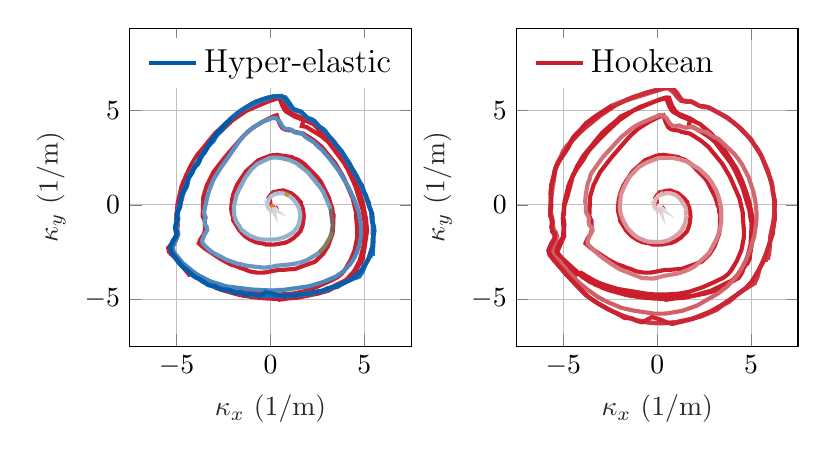
\begin{tikzpicture}

\begin{axis}[%
width=0.295\textwidth,
height=0.333\textwidth,
at={(0\textwidth,0\textwidth)},
scale only axis,
xmin=-7.5,
xmax=7.5,
xlabel style={font=\color{white!15!black}},
xlabel={$\kappa_x$ (1/m)},
ymin=-7.5,
ymax=9.375,
ylabel style={font=\color{white!15!black}},
ylabel={$\kappa_y$ (1/m)},
axis background/.style={fill=white},
xmajorgrids,
ymajorgrids,
legend style={at={(0.03,0.97)}, anchor=north west, legend columns=1, legend cell align=left, align=left, draw=white!15!black},
legend style={font=\fontsize{12}{11}\selectfont, /tikz/every even row/.append style={column sep=0.5cm}, draw=none}
]
\addplot [color=mycolor1, line width=1.5pt]
  table[row sep=crcr]{%
-1.9235	4.7738\\
};
\addlegendentry{Hyper-elastic}

\addplot [color=mycolor2, line width=1.5pt, forget plot]
  table[row sep=crcr]{%
0.38814	-0.11188\\
0.31992	-0.16113\\
0.20852	-0.17867\\
0.139	-0.19331\\
0.0198650000000002	-0.10082\\
-0.00172840000000019	0.0266520000000003\\
-0.0378499999999997	0.33069\\
-0.094074	0.38729\\
-0.0405480000000003	0.47043\\
0.13315	0.66466\\
0.49495	0.74828\\
0.60906	0.75935\\
0.67632	0.76952\\
1.1089	0.61459\\
1.3882	0.38445\\
1.6093	0.13841\\
1.6139	-0.00399040000000017\\
1.6959	-0.10417\\
1.7591	-0.43112\\
1.7717	-0.61284\\
1.7369	-0.93698\\
1.7049	-1.0999\\
1.5905	-1.4009\\
1.4451	-1.5581\\
1.2441	-1.7506\\
0.96396	-1.9294\\
0.76356	-2.0126\\
0.19079	-2.1094\\
-0.24752	-2.1018\\
-0.41926	-2.046\\
-0.77407	-1.9825\\
-1.092	-1.8391\\
-1.3699	-1.6549\\
-1.6537	-1.3563\\
-1.9844	-0.82745\\
-1.9821	-0.71844\\
-2.0749	-0.37693\\
-2.0953	-0.19497\\
-2.0439	0.30147\\
-1.9707	0.59521\\
-1.7873	1.0574\\
-1.3148	1.7713\\
-0.64373	2.3707\\
-0.0742839999999996	2.5913\\
0.12825	2.6415\\
0.22636	2.6278\\
0.33246	2.6572\\
1.1247	2.5358\\
1.2195	2.4784\\
1.4602	2.399\\
1.635	2.2853\\
1.8259	2.1445\\
2.5026	1.4568\\
2.6748	1.2348\\
3.1076	0.38092\\
3.2276	-0.0392849999999996\\
3.2819	-0.14972\\
3.3097	-0.40132\\
3.3559	-0.53005\\
3.3358	-1.1724\\
3.2995	-1.5347\\
3.0519	-2.2045\\
2.8096	-2.5903\\
2.4452	-2.9493\\
2.376	-3.0118\\
1.3166	-3.3968\\
0.68477	-3.4473\\
0.41813	-3.4533\\
-0.32547	-3.5925\\
-0.704	-3.5983\\
-1.1244	-3.5263\\
-1.3962	-3.4081\\
-1.6968	-3.3104\\
-1.8029	-3.2584\\
-2.1169	-3.1626\\
-2.3721	-3.0299\\
-2.6447	-2.8818\\
-3.512	-2.311\\
-3.8204	-2.0389\\
-3.7304	-1.8204\\
-3.5501	-1.5543\\
-3.4851	-1.3378\\
-3.4981	-0.84768\\
-3.6129	-0.60421\\
-3.5784	0.41358\\
-3.4001	1.0208\\
-3.0416	1.7407\\
-2.432	2.5222\\
-1.6677	3.4039\\
-1.4129	3.6852\\
-1.0055	4.0478\\
-0.42635	4.4116\\
0.17571	4.706\\
0.33215	4.7579\\
0.46488	4.3591\\
0.59507	4.1131\\
0.74591	4.0079\\
0.98491	3.9608\\
1.1497	3.9462\\
1.2814	3.8793\\
1.7499	3.7784\\
2.3189	3.417\\
2.7247	3.0818\\
3.4624	2.1876\\
3.8788	1.4839\\
4.3799	0.3484\\
4.5639	-0.44533\\
4.5555	-0.56228\\
4.6202	-1.3627\\
4.6186	-1.7125\\
4.488	-2.3934\\
4.2388	-2.9845\\
3.9387	-3.4798\\
3.7748	-3.6753\\
3.5455	-3.8557\\
3.2964	-3.9743\\
3.0429	-4.0978\\
2.4248	-4.3696\\
1.6998	-4.6111\\
1.1704	-4.7105\\
0.58878	-4.7491\\
-0.0148989999999998	-4.7576\\
-0.43027	-4.7349\\
-2.0747	-4.4683\\
-2.5134	-4.3384\\
-2.8995	-4.2142\\
-3.2524	-4.0689\\
-3.7868	-3.774\\
-4.0484	-3.6059\\
-4.3338	-3.7085\\
-5.0995	-2.7903\\
-5.3337	-2.5154\\
-4.9532	-1.6614\\
-4.9631	-1.2627\\
-4.9392	-1.0561\\
-5.0182	-0.54287\\
-4.9403	-0.033156\\
-4.7647	0.50972\\
-4.481	1.5801\\
-4.2562	2.0681\\
-3.914	2.6346\\
-3.1012	3.5959\\
-1.9445	4.6893\\
-1.1308	5.0629\\
-0.52816	5.3199\\
0.10824	5.5857\\
0.4667	5.6993\\
0.62847	5.6907\\
0.79711	5.2468\\
0.97183	4.975\\
1.1236	4.8439\\
1.7773	4.5766\\
2.0837	4.3777\\
2.2678	4.3008\\
2.8893	3.7782\\
3.1751	3.4516\\
3.4484	3.1383\\
4.2421	1.9001\\
4.5314	1.2585\\
4.7669	0.59886\\
4.9099	0.14369\\
5.0788	-0.71966\\
5.1452	-1.3594\\
4.9712	-2.5126\\
4.7497	-3.1222\\
4.5247	-3.5119\\
4.27	-3.8319\\
4.0597	-4.0108\\
2.9614	-4.5747\\
2.6006	-4.6965\\
1.4353	-4.9272\\
0.54734	-4.9887\\
-0.11799	-4.9751\\
-0.99164	-4.8959\\
-2.0568	-4.6676\\
-2.6913	-4.4881\\
-3.6257	-4.0668\\
-4.1032	-3.7208\\
-4.3753	-3.478\\
-4.6437	-3.2473\\
-5.4067	-2.4937\\
-5.3097	-2.2252\\
-5.0981	-1.9254\\
-5.0138	-1.704\\
-4.9885	-1.1695\\
-5.0139	-0.86223\\
-4.9739	-0.23911\\
-4.933	0.17165\\
-4.6349	1.234\\
-4.3062	1.9158\\
-3.638	2.8695\\
-3.5047	3.1073\\
-2.9104	3.8371\\
-2.4447	4.2546\\
-1.463	4.9067\\
-0.94353	5.1849\\
0.28855	5.647\\
0.46875	5.682\\
0.63017	5.2657\\
0.76945	5.014\\
0.87464	4.9188\\
2.2843	4.2886\\
2.5495	4.0254\\
2.8702	3.7421\\
3.8445	2.4879\\
4.367	1.4534\\
4.6323	0.79366\\
4.8791	0.0112269999999999\\
4.9325	-0.29642\\
5.0421	-0.82594\\
4.9817	-1.9934\\
4.9304	-2.8319\\
4.8013	-3.1226\\
4.6862	-3.1464\\
4.6209	-3.2026\\
4.541	-3.558\\
4.3324	-3.8828\\
3.0556	-4.5658\\
2.5578	-4.7011\\
1.1939	-4.9493\\
0.54906	-4.9764\\
-0.37235	-4.9535\\
-1.4452	-4.8246\\
-2.2996	-4.5966\\
-2.8922	-4.3821\\
-3.2796	-4.2422\\
-3.9506	-3.8478\\
-5.3129	-2.6009\\
-5.4231	-2.4754\\
-5.3918	-2.2717\\
-5.1366	-1.946\\
-5.0143	-1.7059\\
-4.9819	-1.3249\\
-5.0217	-0.67737\\
-4.9732	-0.46801\\
-4.982	-0.29576\\
-4.9529	0.0498659999999997\\
-4.7389	0.98217\\
-4.4747	1.6131\\
-4.1692	2.1413\\
-3.6827	2.8324\\
-3.0806	3.4846\\
-2.7682	3.7954\\
-2.0253	4.4877\\
-1.2865	4.9922\\
-0.42344	5.3766\\
0.0889049999999996	5.5614\\
0.43327	5.6721\\
0.6233	5.3923\\
0.78271	5.0665\\
0.92669	4.9013\\
1.2743	4.691\\
1.7523	4.5038\\
1.67	4.1856\\
1.9105	4.134\\
2.7243	3.6382\\
3.0763	3.339\\
3.9143	2.2283\\
4.145	1.8213\\
4.5232	0.98374\\
4.9197	-0.3192\\
4.9797	-0.78747\\
5.0292	-0.95469\\
4.9994	-1.9963\\
4.8232	-2.699\\
4.7331	-3.0023\\
4.4431	-3.5299\\
4.0924	-3.9206\\
3.969	-4.0204\\
2.8794	-4.5519\\
1.9326	-4.8179\\
0.46844	-5.0358\\
-0.18679	-4.7493\\
-0.5047	-4.723\\
-0.89134	-4.8113\\
-1.6252	-4.7883\\
-2.5555	-4.5309\\
-2.9436	-4.3944\\
-3.261	-4.207\\
-3.622	-4.072\\
-3.941	-3.8247\\
-4.2342	-3.5792\\
-5.0622	-2.8388\\
-5.4064	-2.4503\\
-5.452	-2.2889\\
-5.1658	-1.9374\\
-5.007	-1.6863\\
-4.9711	-1.4786\\
-5.029	-0.70034\\
-4.9632	-0.49217\\
-4.947	0.0406899999999997\\
-4.7887	0.72884\\
-4.6499	1.2141\\
-4.2871	1.9004\\
-3.9223	2.4028\\
-3.6479	2.9136\\
-3.3631	3.3029\\
-2.9329	3.8192\\
-2.3112	4.3335\\
-1.8426	4.6824\\
-1.645	4.7986\\
};
\addplot [color=mycolor4, line width=1.5pt, forget plot]
  table[row sep=crcr]{%
0	0\\
0.16795	-0.13327\\
};
\addplot [color=mycolor5, line width=1.5pt, forget plot]
  table[row sep=crcr]{%
0.16795	-0.13327\\
0.36965	-0.29457\\
};
\addplot [color=mycolor6, line width=1.5pt, forget plot]
  table[row sep=crcr]{%
0.36965	-0.29457\\
0.30269	-0.24715\\
};
\addplot [color=mycolor7, line width=1.5pt, forget plot]
  table[row sep=crcr]{%
0.30269	-0.24715\\
0.18227	-0.16224\\
0.22934	-0.21005\\
};
\addplot [color=mycolor8, line width=1.5pt, forget plot]
  table[row sep=crcr]{%
0.22934	-0.21005\\
0.30853	-0.28166\\
0.26763	-0.26427\\
};
\addplot [color=mycolor9, line width=1.5pt, forget plot]
  table[row sep=crcr]{%
0.26763	-0.26427\\
0.19605	-0.24186\\
};
\addplot [color=mycolor10, line width=1.5pt, forget plot]
  table[row sep=crcr]{%
0.19605	-0.24186\\
0.24194	-0.30882\\
};
\addplot [color=mycolor11, line width=1.5pt, forget plot]
  table[row sep=crcr]{%
0.24194	-0.30882\\
0.17062	-0.27117\\
0.16467	-0.31619\\
};
\addplot [color=mycolor12, line width=1.5pt, forget plot]
  table[row sep=crcr]{%
0.16467	-0.31619\\
0.18125	-0.34728\\
0.17633	-0.31618\\
};
\addplot [color=mycolor13, line width=1.5pt, forget plot]
  table[row sep=crcr]{%
0.17633	-0.31618\\
0.1497	-0.29086\\
0.10815	-0.3264\\
};
\addplot [color=mycolor14, line width=1.5pt, forget plot]
  table[row sep=crcr]{%
0.10815	-0.3264\\
0.075455	-0.30193\\
};
\addplot [color=mycolor15, line width=1.5pt, forget plot]
  table[row sep=crcr]{%
0.075455	-0.30193\\
0.040891	-0.32102\\
0.039125	-0.30687\\
};
\addplot [color=mycolor16, line width=1.5pt, forget plot]
  table[row sep=crcr]{%
0.039125	-0.30687\\
-0.019649	-0.28334\\
-0.020954	-0.2864\\
};
\addplot [color=mycolor17, line width=1.5pt, forget plot]
  table[row sep=crcr]{%
-0.020954	-0.2864\\
-0.045133	-0.248\\
};
\addplot [color=mycolor18, line width=1.5pt, forget plot]
  table[row sep=crcr]{%
-0.045133	-0.248\\
-0.085551	-0.20372\\
-0.081886	-0.21525\\
};
\addplot [color=mycolor19, line width=1.5pt, forget plot]
  table[row sep=crcr]{%
-0.081886	-0.21525\\
-0.13202	-0.14435\\
-0.13597	-0.15255\\
};
\addplot [color=mycolor20, line width=1.5pt, forget plot]
  table[row sep=crcr]{%
-0.13597	-0.15255\\
-0.15293	-0.073254\\
-0.15019	-0.066166\\
};
\addplot [color=mycolor1!10!mycolor12, line width=1.5pt, forget plot]
  table[row sep=crcr]{%
-0.15019	-0.066166\\
-0.16771	0.00604299999999999\\
-0.16792	0.00670319999999999\\
};
\addplot [color=mycolor21, line width=1.5pt, forget plot]
  table[row sep=crcr]{%
-0.16792	0.00670319999999999\\
-0.16518	0.12138\\
-0.15225	0.12286\\
};
\addplot [color=mycolor22, line width=1.5pt, forget plot]
  table[row sep=crcr]{%
-0.15225	0.12286\\
-0.093467	0.28922\\
};
\addplot [color=mycolor23, line width=1.5pt, forget plot]
  table[row sep=crcr]{%
-0.093467	0.28922\\
-0.054226	0.34864\\
-0.021773	0.3883\\
};
\addplot [color=mycolor24, line width=1.5pt, forget plot]
  table[row sep=crcr]{%
-0.021773	0.3883\\
0.052968	0.47753\\
0.089042	0.49125\\
};
\addplot [color=mycolor1!20!mycolor7, line width=1.5pt, forget plot]
  table[row sep=crcr]{%
0.089042	0.49125\\
0.21453	0.56242\\
};
\addplot [color=mycolor25, line width=1.5pt, forget plot]
  table[row sep=crcr]{%
0.21453	0.56242\\
0.38261	0.61323\\
};
\addplot [color=mycolor26, line width=1.5pt, forget plot]
  table[row sep=crcr]{%
0.38261	0.61323\\
0.59174	0.62227\\
};
\addplot [color=mycolor27, line width=1.5pt, forget plot]
  table[row sep=crcr]{%
0.59174	0.62227\\
0.69959	0.60465\\
0.77076	0.58937\\
};
\addplot [color=mycolor1!25!mycolor6, line width=1.5pt, forget plot]
  table[row sep=crcr]{%
0.77076	0.58937\\
0.95975	0.50934\\
0.9961	0.47988\\
};
\addplot [color=mycolor28, line width=1.5pt, forget plot]
  table[row sep=crcr]{%
0.9961	0.47988\\
1.2079	0.30662\\
};
\addplot [color=mycolor29, line width=1.5pt, forget plot]
  table[row sep=crcr]{%
1.2079	0.30662\\
1.3575	0.11682\\
1.3874	0.0630330000000001\\
};
\addplot [color=mycolor1!25!mycolor10, line width=1.5pt, forget plot]
  table[row sep=crcr]{%
1.3874	0.0630330000000001\\
1.4681	-0.0644439999999999\\
1.5166	-0.16298\\
1.52	-0.25194\\
};
\addplot [color=mycolor1!20!mycolor17, line width=1.5pt, forget plot]
  table[row sep=crcr]{%
1.52	-0.25194\\
1.5582	-0.34276\\
1.5956	-0.57537\\
};
\addplot [color=mycolor30, line width=1.5pt, forget plot]
  table[row sep=crcr]{%
1.5956	-0.57537\\
1.5228	-0.98094\\
};
\addplot [color=mycolor1!25!mycolor14, line width=1.5pt, forget plot]
  table[row sep=crcr]{%
1.5228	-0.98094\\
1.4099	-1.2218\\
1.2884	-1.3477\\
};
\addplot [color=mycolor31, line width=1.5pt, forget plot]
  table[row sep=crcr]{%
1.2884	-1.3477\\
1.222	-1.44\\
0.94165	-1.626\\
};
\addplot [color=mycolor1!20!mycolor21, line width=1.5pt, forget plot]
  table[row sep=crcr]{%
0.94165	-1.626\\
0.56934	-1.7785\\
};
\addplot [color=mycolor1!30!mycolor12, line width=1.5pt, forget plot]
  table[row sep=crcr]{%
0.56934	-1.7785\\
0.30873	-1.8292\\
0.0668740000000001	-1.8434\\
};
\addplot [color=mycolor32, line width=1.5pt, forget plot]
  table[row sep=crcr]{%
0.0668740000000001	-1.8434\\
-0.22619	-1.8467\\
-0.56645	-1.8266\\
};
\addplot [color=mycolor33, line width=1.5pt, forget plot]
  table[row sep=crcr]{%
-0.56645	-1.8266\\
-0.82749	-1.7589\\
-0.85459	-1.7286\\
-1.1159	-1.6468\\
};
\addplot [color=mycolor1!25!mycolor21, line width=1.5pt, forget plot]
  table[row sep=crcr]{%
-1.1159	-1.6468\\
-1.2703	-1.5251\\
-1.3611	-1.4841\\
-1.3869	-1.4292\\
-1.6121	-1.2747\\
};
\addplot [color=mycolor34, line width=1.5pt, forget plot]
  table[row sep=crcr]{%
-1.6121	-1.2747\\
-1.6428	-1.1443\\
-1.8014	-0.9295\\
-1.9148	-0.64756\\
};
\addplot [color=mycolor35, line width=1.5pt, forget plot]
  table[row sep=crcr]{%
-1.9148	-0.64756\\
-1.9382	-0.49282\\
-1.9537	-0.11798\\
-1.8947	0.14278\\
};
\addplot [color=mycolor1!40!mycolor7, line width=1.5pt, forget plot]
  table[row sep=crcr]{%
-1.8947	0.14278\\
-1.8243	0.49221\\
-1.6808	0.80259\\
};
\addplot [color=mycolor1!30!mycolor21, line width=1.5pt, forget plot]
  table[row sep=crcr]{%
-1.6808	0.80259\\
-1.3405	1.4536\\
-1.271	1.543\\
};
\addplot [color=mycolor36, line width=1.5pt, forget plot]
  table[row sep=crcr]{%
-1.271	1.543\\
-1.0326	1.8712\\
-0.72401	2.1554\\
-0.61907	2.2158\\
};
\addplot [color=mycolor1!40!mycolor12, line width=1.5pt, forget plot]
  table[row sep=crcr]{%
-0.61907	2.2158\\
-0.0492910000000002	2.4846\\
0.15637	2.5119\\
0.26424	2.5136\\
};
\addplot [color=mycolor37, line width=1.5pt, forget plot]
  table[row sep=crcr]{%
0.26424	2.5136\\
0.5021	2.4985\\
0.99834	2.3787\\
1.1781	2.3055\\
};
\addplot [color=mycolor1!35!mycolor21, line width=1.5pt, forget plot]
  table[row sep=crcr]{%
1.1781	2.3055\\
1.3866	2.2082\\
1.865	1.83\\
2.0338	1.6832\\
};
\addplot [color=mycolor1!40!mycolor17, line width=1.5pt, forget plot]
  table[row sep=crcr]{%
2.0338	1.6832\\
2.6942	0.87041\\
};
\addplot [color=mycolor38, line width=1.5pt, forget plot]
  table[row sep=crcr]{%
2.6942	0.87041\\
2.8195	0.66974\\
3.2037	-0.22125\\
};
\addplot [color=mycolor1!50!mycolor4, line width=1.5pt, forget plot]
  table[row sep=crcr]{%
3.2037	-0.22125\\
3.3127	-1.0906\\
3.2605	-1.4582\\
};
\addplot [color=mycolor1!50!mycolor6, line width=1.5pt, forget plot]
  table[row sep=crcr]{%
3.2605	-1.4582\\
3.1624	-1.7383\\
2.9136	-2.1735\\
2.5774	-2.5563\\
};
\addplot [color=mycolor1!50!mycolor8, line width=1.5pt, forget plot]
  table[row sep=crcr]{%
2.5774	-2.5563\\
1.9348	-2.9365\\
1.6905	-3.0245\\
1.4832	-3.0855\\
};
\addplot [color=mycolor1!50!mycolor10, line width=1.5pt, forget plot]
  table[row sep=crcr]{%
1.4832	-3.0855\\
1.1298	-3.1488\\
0.79003	-3.1857\\
0.30185	-3.2304\\
0.061242	-3.2892\\
};
\addplot [color=mycolor1!50!mycolor12, line width=1.5pt, forget plot]
  table[row sep=crcr]{%
0.061242	-3.2892\\
-0.33324	-3.3327\\
-1.2329	-3.24\\
-1.4825	-3.1747\\
};
\addplot [color=mycolor1!50!mycolor14, line width=1.5pt, forget plot]
  table[row sep=crcr]{%
-1.4825	-3.1747\\
-1.7672	-3.1201\\
-2.0347	-3.023\\
-2.3286	-2.922\\
-3.0379	-2.5523\\
};
\addplot [color=mycolor1!50!mycolor16, line width=1.5pt, forget plot]
  table[row sep=crcr]{%
-3.0379	-2.5523\\
-3.2953	-2.3651\\
-3.6147	-2.0452\\
-3.6371	-1.8789\\
-3.5232	-1.6004\\
-3.3707	-1.3365\\
-3.3909	-1.1817\\
-3.5074	-1.0473\\
-3.5122	-0.86206\\
};
\addplot [color=mycolor1!50!mycolor18, line width=1.5pt, forget plot]
  table[row sep=crcr]{%
-3.5122	-0.86206\\
-3.4546	-0.6847\\
-3.5445	-0.40981\\
-3.3617	0.45274\\
-3.2942	0.69848\\
};
\addplot [color=mycolor1!50!mycolor20, line width=1.5pt, forget plot]
  table[row sep=crcr]{%
-3.2942	0.69848\\
-3.0396	1.3378\\
-2.6843	1.9192\\
-2.509	2.1645\\
};
\addplot [color=mycolor1!50!mycolor21, line width=1.5pt, forget plot]
  table[row sep=crcr]{%
-2.509	2.1645\\
-1.6178	3.4426\\
-1.2253	3.8774\\
};
\addplot [color=mycolor1!50!mycolor23, line width=1.5pt, forget plot]
  table[row sep=crcr]{%
-1.2253	3.8774\\
-0.90277	4.1171\\
-0.41774	4.4137\\
0.10443	4.6068\\
0.2859	4.6063\\
0.47328	4.4409\\
0.64568	4.1566\\
0.81693	4.0064\\
};
\addplot [color=mycolor1!60!mycolor7, line width=1.5pt, forget plot]
  table[row sep=crcr]{%
0.81693	4.0064\\
0.98495	4.0223\\
1.1249	3.9826\\
1.2659	3.8628\\
1.4409	3.806\\
1.6154	3.7962\\
1.7527	3.7192\\
1.8791	3.5923\\
2.2936	3.33\\
2.533	3.0992\\
};
\addplot [color=mycolor1!50!mycolor26, line width=1.5pt, forget plot]
  table[row sep=crcr]{%
2.533	3.0992\\
2.7554	2.9021\\
3.1782	2.4189\\
3.6526	1.7819\\
3.7388	1.6405\\
};
\addplot [color=mycolor1!60!mycolor12, line width=1.5pt, forget plot]
  table[row sep=crcr]{%
3.7388	1.6405\\
4.1631	0.91409\\
4.4629	0.27683\\
4.6313	-0.19217\\
4.6958	-0.39542\\
};
\addplot [color=mycolor1!50!mycolor29, line width=1.5pt, forget plot]
  table[row sep=crcr]{%
4.6958	-0.39542\\
4.8034	-0.97007\\
4.8286	-1.5669\\
4.7284	-2.1572\\
4.602	-2.5149\\
4.4405	-2.8568\\
};
\addplot [color=mycolor1!60!mycolor17, line width=1.5pt, forget plot]
  table[row sep=crcr]{%
4.4405	-2.8568\\
4.2474	-3.1404\\
3.8995	-3.514\\
3.4857	-3.803\\
2.8068	-4.0941\\
};
\addplot [color=mycolor1!56!mycolor25, line width=1.5pt, forget plot]
  table[row sep=crcr]{%
2.8068	-4.0941\\
2.0754	-4.3147\\
0.66426	-4.5179\\
0.50943	-4.5089\\
0.17676	-4.5474\\
};
\addplot [color=mycolor1!60!mycolor21, line width=1.5pt, forget plot]
  table[row sep=crcr]{%
0.17676	-4.5474\\
-0.31803	-4.5297\\
-1.0429	-4.4883\\
-2.1881	-4.3481\\
-2.3773	-4.3163\\
};
\addplot [color=mycolor1!50!mycolor32, line width=1.5pt, forget plot]
  table[row sep=crcr]{%
-2.3773	-4.3163\\
-3.1804	-4.0701\\
-3.9139	-3.7072\\
-4.6592	-3.1044\\
-4.8017	-2.9327\\
};
\addplot [color=mycolor1!60!mycolor25, line width=1.5pt, forget plot]
  table[row sep=crcr]{%
-4.8017	-2.9327\\
-5.0869	-2.5978\\
-5.1817	-2.4334\\
-5.1882	-2.1876\\
-4.9106	-1.5412\\
-5.0138	-1.1654\\
-4.9066	-0.70868\\
-4.9408	-0.5451\\
-4.9396	-0.30626\\
-4.8453	0.0182419999999999\\
-4.7482	0.22052\\
};
\addplot [color=mycolor1!50!mycolor35, line width=1.5pt, forget plot]
  table[row sep=crcr]{%
-4.7482	0.22052\\
-4.7146	0.28851\\
-4.6941	0.4414\\
-4.5991	0.69941\\
-4.4652	0.95609\\
-4.3145	1.5598\\
-4.022	2.0872\\
-3.9435	2.285\\
-3.7113	2.5254\\
-3.6497	2.6905\\
-3.5365	2.8496\\
};
\addplot [color=mycolor1!65!mycolor21, line width=1.5pt, forget plot]
  table[row sep=crcr]{%
-3.5365	2.8496\\
-3.4002	2.9815\\
-3.0841	3.439\\
-2.8363	3.7522\\
-2.5759	4.0765\\
-2.072	4.6324\\
-1.6943	4.937\\
};
\addplot [color=mycolor1!70!mycolor12, line width=1.5pt, forget plot]
  table[row sep=crcr]{%
-1.6943	4.937\\
-0.54228	5.514\\
-0.29848	5.5769\\
0.10721	5.7346\\
0.55915	5.756\\
0.79479	5.7084\\
0.98903	5.4444\\
1.1915	5.106\\
1.4201	4.976\\
};
\addplot [color=mycolor1!60!mycolor31, line width=1.5pt, forget plot]
  table[row sep=crcr]{%
1.4201	4.976\\
1.617	4.9515\\
1.9536	4.6058\\
2.3035	4.4534\\
2.6106	4.1475\\
2.7645	4.0439\\
3.5094	3.1729\\
};
\addplot [color=mycolor1!50!mycolor38, line width=1.5pt, forget plot]
  table[row sep=crcr]{%
3.5094	3.1729\\
3.7088	2.9036\\
4.3694	1.9038\\
4.7307	1.245\\
4.9744	0.72639\\
};
\addplot [color=mycolor1!75!mycolor6, line width=1.5pt, forget plot]
  table[row sep=crcr]{%
4.9744	0.72639\\
5.2585	-0.0683600000000002\\
5.3892	-0.45354\\
5.4887	-1.345\\
5.4222	-2.2058\\
5.3534	-2.418\\
};
\addplot [color=mycolor1!75!mycolor10, line width=1.5pt, forget plot]
  table[row sep=crcr]{%
5.3534	-2.418\\
5.2339	-2.8151\\
4.9455	-3.3285\\
4.5878	-3.7349\\
4.3042	-3.9403\\
4.0169	-4.1053\\
3.5811	-4.3085\\
2.8698	-4.5091\\
};
\addplot [color=mycolor1!75!mycolor14, line width=1.5pt, forget plot]
  table[row sep=crcr]{%
2.8698	-4.5091\\
2.6028	-4.6232\\
2.1643	-4.6155\\
2.0459	-4.7089\\
1.84	-4.7609\\
1.6094	-4.7252\\
1.4455	-4.7408\\
1.2819	-4.8126\\
1.0639	-4.8165\\
0.86481	-4.7835\\
0.52796	-4.8511\\
0.13235	-4.8093\\
-0.0417540000000001	-4.8395\\
};
\addplot [color=mycolor1!75!mycolor18, line width=1.5pt, forget plot]
  table[row sep=crcr]{%
-0.0417540000000001	-4.8395\\
-0.22517	-4.841\\
-0.6032	-4.792\\
-0.77266	-4.8084\\
-1.3393	-4.7206\\
-1.523	-4.7055\\
-1.9212	-4.6088\\
-2.2791	-4.5504\\
-2.7211	-4.4167\\
-2.9355	-4.3736\\
};
\addplot [color=mycolor1!75!mycolor21, line width=1.5pt, forget plot]
  table[row sep=crcr]{%
-2.9355	-4.3736\\
-3.5318	-4.1149\\
-4.1062	-3.7523\\
-4.304	-3.613\\
-4.6247	-3.3166\\
-4.799	-3.1869\\
-4.9429	-3.0227\\
-5.1954	-2.6329\\
-5.3186	-2.4667\\
-5.3119	-2.2469\\
-5.1357	-1.9232\\
};
\addplot [color=mycolor1!80!mycolor7, line width=1.5pt, forget plot]
  table[row sep=crcr]{%
-5.1357	-1.9232\\
-5.0043	-1.6203\\
-5.0841	-1.2727\\
-4.9693	-0.83728\\
-4.9971	-0.67788\\
-4.982	-0.50437\\
-4.8463	-0.0498310000000002\\
-4.7925	0.2749\\
-4.6857	0.63119\\
-4.493	1.041\\
-4.4471	1.236\\
-4.3571	1.4218\\
};
\addplot [color=mycolor1!80!mycolor12, line width=1.5pt, forget plot]
  table[row sep=crcr]{%
-4.3571	1.4218\\
-4.2482	1.5684\\
-4.1331	1.8579\\
-3.8308	2.2842\\
-3.0774	3.5457\\
-2.832	3.8246\\
-2.6969	3.985\\
};
\addplot [color=mycolor1!80!mycolor17, line width=1.5pt, forget plot]
  table[row sep=crcr]{%
-2.6969	3.985\\
-2.4286	4.2748\\
-1.5813	5.0049\\
-1.1774	5.2457\\
-0.76814	5.4925\\
-0.10633	5.702\\
0.34834	5.7745\\
};
\addplot [color=mycolor1!80!mycolor21, line width=1.5pt, forget plot]
  table[row sep=crcr]{%
0.34834	5.7745\\
0.55557	5.7339\\
0.78891	5.5497\\
1.1774	5.0716\\
1.3623	5.0521\\
1.6121	4.9432\\
1.9838	4.6025\\
2.1436	4.568\\
2.3353	4.454\\
2.6207	4.1226\\
2.7613	4.0498\\
2.9157	3.9158\\
3.1522	3.5948\\
3.2754	3.4903\\
};
\addplot [color=mycolor1!80!mycolor25, line width=1.5pt, forget plot]
  table[row sep=crcr]{%
3.2754	3.4903\\
3.8674	2.698\\
4.811	1.0865\\
4.8895	0.91305\\
};
\addplot [color=mycolor1!80!mycolor29, line width=1.5pt, forget plot]
  table[row sep=crcr]{%
4.8895	0.91305\\
5.0276	0.60258\\
5.0866	0.50932\\
5.1967	0.0866569999999998\\
5.3597	-0.32578\\
5.3885	-0.83312\\
5.4407	-1.0143\\
5.4463	-1.1919\\
5.436	-1.513\\
5.4909	-1.5445\\
5.4922	-1.8315\\
5.4413	-2.7119\\
};
\addplot [color=mycolor1!80!mycolor31, line width=1.5pt, forget plot]
  table[row sep=crcr]{%
5.4413	-2.7119\\
5.285	-2.7117\\
5.051	-3.1933\\
4.9071	-3.5435\\
4.7176	-3.8162\\
4.3729	-3.9339\\
3.9045	-4.1406\\
3.5561	-4.3612\\
3.2177	-4.3877\\
2.9851	-4.5323\\
2.7536	-4.6121\\
2.58	-4.5668\\
2.4321	-4.6166\\
2.2347	-4.7407\\
};
\addplot [color=mycolor1!85!mycolor21, line width=1.5pt, forget plot]
  table[row sep=crcr]{%
2.2347	-4.7407\\
2.0029	-4.7298\\
1.8174	-4.6838\\
1.6702	-4.7694\\
1.4827	-4.83\\
1.2563	-4.7716\\
1.069	-4.7761\\
0.91706	-4.8593\\
0.72204	-4.8415\\
0.4997	-4.7837\\
0.1569	-4.8641\\
-0.040959	-4.8112\\
-0.24161	-4.7983\\
-0.41786	-4.8355\\
-0.96431	-4.7631\\
};
\addplot [color=mycolor1!80!mycolor36, line width=1.5pt, forget plot]
  table[row sep=crcr]{%
-0.96431	-4.7631\\
-1.1499	-4.763\\
-1.5143	-4.668\\
-1.706	-4.6707\\
-2.5265	-4.4978\\
-2.9259	-4.3391\\
-3.1512	-4.2989\\
-3.338	-4.2286\\
-3.7245	-3.9775\\
-4.1294	-3.7391\\
-4.2844	-3.597\\
};
\addplot [color=mycolor1!80!mycolor38, line width=1.5pt, forget plot]
  table[row sep=crcr]{%
-4.2844	-3.597\\
-4.6705	-3.289\\
-5.0732	-2.7922\\
-5.3151	-2.4297\\
-5.3182	-2.2215\\
-5.022	-1.621\\
-5.0091	-1.4182\\
-5.0532	-1.2544\\
-4.9651	-0.49022\\
-4.9175	-0.29335\\
};
\addplot [color=mycolor1!90!mycolor12, line width=1.5pt, forget plot]
  table[row sep=crcr]{%
-4.9175	-0.29335\\
-4.7783	0.1743\\
-4.698	0.54653\\
-4.5831	0.88346\\
-4.4207	1.2308\\
-4.3537	1.4521\\
-4.0997	1.88\\
-4.0145	2.0578\\
-3.7984	2.3321\\
-3.7414	2.4982\\
-3.6369	2.6509\\
-3.4939	2.7817\\
-3.3242	3.1053\\
};
\addplot [color=mycolor1!90!mycolor21, line width=1.5pt, forget plot]
  table[row sep=crcr]{%
-3.3242	3.1053\\
-3.0375	3.3903\\
-2.8402	3.7345\\
-2.6703	3.8717\\
-2.5268	4.0388\\
-2.4154	4.2247\\
-1.7387	4.886\\
-1.3775	5.1402\\
-0.95363	5.3951\\
-0.30183	5.6475\\
};
\addplot [color=mycolor1!90!mycolor29, line width=1.5pt, forget plot]
  table[row sep=crcr]{%
-0.30183	5.6475\\
0.11862	5.7479\\
0.58241	5.7819\\
0.80338	5.653\\
1.2507	5.0414\\
1.6495	4.9301\\
1.9894	4.5924\\
2.1698	4.5417\\
2.3481	4.4352\\
2.6307	4.1156\\
2.7807	4.0363\\
2.9199	3.9017\\
3.0401	3.7249\\
};
\addplot [color=mycolor1!92!mycolor25, line width=1.5pt, forget plot]
  table[row sep=crcr]{%
3.0401	3.7249\\
3.4095	3.3163\\
3.5124	3.1545\\
3.782	2.8695\\
4.0753	2.392\\
4.198	2.2258\\
4.3646	1.8939\\
4.5698	1.5714\\
4.7366	1.2368\\
4.8566	1.0556\\
4.9294	0.87586\\
};
\addplot [color=mycolor1!90!mycolor38, line width=1.5pt, forget plot]
  table[row sep=crcr]{%
4.9294	0.87586\\
4.96	0.70849\\
5.2297	0.12491\\
5.2498	-0.0757500000000002\\
5.424	-0.49823\\
5.4396	-0.91884\\
5.5088	-1.1527\\
5.5387	-1.3882\\
5.4452	-1.8094\\
5.4602	-2.0354\\
5.4285	-2.2547\\
5.2887	-2.6454\\
5.2507	-2.8428\\
};
\addplot [color=mycolor1!95!mycolor21, line width=1.5pt, forget plot]
  table[row sep=crcr]{%
5.2507	-2.8428\\
4.8361	-3.4898\\
4.2477	-3.9819\\
3.4452	-4.338\\
3.0286	-4.4271\\
2.8231	-4.5292\\
2.5446	-4.6141\\
2.1994	-4.6406\\
1.9999	-4.7242\\
1.5822	-4.7214\\
};
\addplot [color=mycolor1!96!mycolor25, line width=1.5pt, forget plot]
  table[row sep=crcr]{%
1.5822	-4.7214\\
1.252	-4.8223\\
0.84602	-4.7897\\
0.67009	-4.8664\\
0.0745310000000003	-4.697\\
-0.26783	-4.6344\\
-0.45061	-4.7657\\
-0.65452	-4.8465\\
-0.90683	-4.745\\
-1.0904	-4.7251\\
-1.2244	-4.8086\\
-1.4009	-4.7472\\
-1.6062	-4.6365\\
-1.7825	-4.6711\\
};
\addplot [color=mycolor1!96!mycolor38, line width=1.5pt, forget plot]
  table[row sep=crcr]{%
-1.7825	-4.6711\\
-1.9409	-4.6729\\
-2.1218	-4.5401\\
-2.3343	-4.4821\\
-2.5562	-4.5107\\
-2.7567	-4.4365\\
-2.9507	-4.3126\\
-3.3158	-4.2604\\
-3.738	-3.9391\\
-3.9467	-3.8743\\
-4.119	-3.7738\\
-4.5021	-3.4058\\
-4.6733	-3.2995\\
-4.9506	-2.9455\\
-5.2238	-2.6049\\
};
\addplot [color=mycolor1!98!mycolor38, line width=1.5pt, forget plot]
  table[row sep=crcr]{%
-5.2238	-2.6049\\
-5.3105	-2.4308\\
-5.3398	-2.2071\\
-5.2108	-1.9133\\
-5.0188	-1.6146\\
-5.0004	-1.4058\\
-5.0904	-1.2365\\
-5.0528	-1.0232\\
-4.9457	-0.80834\\
-4.9939	-0.49217\\
-4.8023	-0.0791599999999999\\
-4.7914	0.18236\\
-4.736	0.55128\\
-4.431	1.0706\\
-4.4263	1.2262\\
-4.3791	1.452\\
-4.2405	1.6207\\
};
\addplot [color=mycolor1, line width=1.5pt, forget plot]
  table[row sep=crcr]{%
-4.2405	1.6207\\
-4.1596	1.7023\\
-4.1329	1.8322\\
-4.0211	2.015\\
-3.8735	2.1529\\
-3.8011	2.28\\
-3.7404	2.4791\\
-3.4958	2.8858\\
-2.9453	3.7038\\
-2.394	4.3208\\
-2.0756	4.6136\\
};
\end{axis}

\begin{axis}[%
width=0.295\textwidth,
height=0.333\textwidth,
at={(0.405\textwidth,0\textwidth)},
scale only axis,
xmin=-7.5,
xmax=7.5,
xlabel style={font=\color{white!15!black}},
xlabel={$\kappa_x$ (1/m)},
ymin=-7.5,
ymax=9.375,
ylabel style={font=\color{white!15!black}},
ylabel={$\kappa_y$ (1/m)},
axis background/.style={fill=white},
xmajorgrids,
ymajorgrids,
legend style={at={(0.03,0.97)}, anchor=north west, legend columns=1, legend cell align=left, align=left, draw=white!15!black},
legend style={font=\fontsize{12}{11}\selectfont, /tikz/every even row/.append style={column sep=0.5cm}, draw=none}
]
\addplot [color=mycolor39, line width=1.5pt]
  table[row sep=crcr]{%
-1.9235	4.7738\\
};
\addlegendentry{Hookean}

\addplot [color=mycolor2, line width=1.5pt, forget plot]
  table[row sep=crcr]{%
0.38814	-0.11188\\
0.31992	-0.16113\\
0.20852	-0.17867\\
0.139	-0.19331\\
0.0198650000000002	-0.10082\\
-0.00172840000000019	0.0266520000000003\\
-0.0378499999999997	0.33069\\
-0.094074	0.38729\\
-0.0405480000000003	0.47043\\
0.13315	0.66466\\
0.49495	0.74828\\
0.60906	0.75935\\
0.67632	0.76952\\
1.1089	0.61459\\
1.3882	0.38445\\
1.6093	0.13841\\
1.6139	-0.00399040000000017\\
1.6959	-0.10417\\
1.7591	-0.43112\\
1.7717	-0.61284\\
1.7369	-0.93698\\
1.7049	-1.0999\\
1.5905	-1.4009\\
1.4451	-1.5581\\
1.2441	-1.7506\\
0.96396	-1.9294\\
0.76356	-2.0126\\
0.19079	-2.1094\\
-0.24752	-2.1018\\
-0.41926	-2.046\\
-0.77407	-1.9825\\
-1.092	-1.8391\\
-1.3699	-1.6549\\
-1.6537	-1.3563\\
-1.9844	-0.82745\\
-1.9821	-0.71844\\
-2.0749	-0.37693\\
-2.0953	-0.19497\\
-2.0439	0.30147\\
-1.9707	0.59521\\
-1.7873	1.0574\\
-1.3148	1.7713\\
-0.64373	2.3707\\
-0.0742839999999996	2.5913\\
0.12825	2.6415\\
0.22636	2.6278\\
0.33246	2.6572\\
1.1247	2.5358\\
1.2195	2.4784\\
1.4602	2.399\\
1.635	2.2853\\
1.8259	2.1445\\
2.5026	1.4568\\
2.6748	1.2348\\
3.1076	0.38092\\
3.2276	-0.0392849999999996\\
3.2819	-0.14972\\
3.3097	-0.40132\\
3.3559	-0.53005\\
3.3358	-1.1724\\
3.2995	-1.5347\\
3.0519	-2.2045\\
2.8096	-2.5903\\
2.4452	-2.9493\\
2.376	-3.0118\\
1.3166	-3.3968\\
0.68477	-3.4473\\
0.41813	-3.4533\\
-0.32547	-3.5925\\
-0.704	-3.5983\\
-1.1244	-3.5263\\
-1.3962	-3.4081\\
-1.6968	-3.3104\\
-1.8029	-3.2584\\
-2.1169	-3.1626\\
-2.3721	-3.0299\\
-2.6447	-2.8818\\
-3.512	-2.311\\
-3.8204	-2.0389\\
-3.7304	-1.8204\\
-3.5501	-1.5543\\
-3.4851	-1.3378\\
-3.4981	-0.84768\\
-3.6129	-0.60421\\
-3.5784	0.41358\\
-3.4001	1.0208\\
-3.0416	1.7407\\
-2.432	2.5222\\
-1.6677	3.4039\\
-1.4129	3.6852\\
-1.0055	4.0478\\
-0.42635	4.4116\\
0.17571	4.706\\
0.33215	4.7579\\
0.46488	4.3591\\
0.59507	4.1131\\
0.74591	4.0079\\
0.98491	3.9608\\
1.1497	3.9462\\
1.2814	3.8793\\
1.7499	3.7784\\
2.3189	3.417\\
2.7247	3.0818\\
3.4624	2.1876\\
3.8788	1.4839\\
4.3799	0.3484\\
4.5639	-0.44533\\
4.5555	-0.56228\\
4.6202	-1.3627\\
4.6186	-1.7125\\
4.488	-2.3934\\
4.2388	-2.9845\\
3.9387	-3.4798\\
3.7748	-3.6753\\
3.5455	-3.8557\\
3.2964	-3.9743\\
3.0429	-4.0978\\
2.4248	-4.3696\\
1.6998	-4.6111\\
1.1704	-4.7105\\
0.58878	-4.7491\\
-0.0148989999999998	-4.7576\\
-0.43027	-4.7349\\
-2.0747	-4.4683\\
-2.5134	-4.3384\\
-2.8995	-4.2142\\
-3.2524	-4.0689\\
-3.7868	-3.774\\
-4.0484	-3.6059\\
-4.3338	-3.7085\\
-5.0995	-2.7903\\
-5.3337	-2.5154\\
-4.9532	-1.6614\\
-4.9631	-1.2627\\
-4.9392	-1.0561\\
-5.0182	-0.54287\\
-4.9403	-0.033156\\
-4.7647	0.50972\\
-4.481	1.5801\\
-4.2562	2.0681\\
-3.914	2.6346\\
-3.1012	3.5959\\
-1.9445	4.6893\\
-1.1308	5.0629\\
-0.52816	5.3199\\
0.10824	5.5857\\
0.4667	5.6993\\
0.62847	5.6907\\
0.79711	5.2468\\
0.97183	4.975\\
1.1236	4.8439\\
1.7773	4.5766\\
2.0837	4.3777\\
2.2678	4.3008\\
2.8893	3.7782\\
3.1751	3.4516\\
3.4484	3.1383\\
4.2421	1.9001\\
4.5314	1.2585\\
4.7669	0.59886\\
4.9099	0.14369\\
5.0788	-0.71966\\
5.1452	-1.3594\\
4.9712	-2.5126\\
4.7497	-3.1222\\
4.5247	-3.5119\\
4.27	-3.8319\\
4.0597	-4.0108\\
2.9614	-4.5747\\
2.6006	-4.6965\\
1.4353	-4.9272\\
0.54734	-4.9887\\
-0.11799	-4.9751\\
-0.99164	-4.8959\\
-2.0568	-4.6676\\
-2.6913	-4.4881\\
-3.6257	-4.0668\\
-4.1032	-3.7208\\
-4.3753	-3.478\\
-4.6437	-3.2473\\
-5.4067	-2.4937\\
-5.3097	-2.2252\\
-5.0981	-1.9254\\
-5.0138	-1.704\\
-4.9885	-1.1695\\
-5.0139	-0.86223\\
-4.9739	-0.23911\\
-4.933	0.17165\\
-4.6349	1.234\\
-4.3062	1.9158\\
-3.638	2.8695\\
-3.5047	3.1073\\
-2.9104	3.8371\\
-2.4447	4.2546\\
-1.463	4.9067\\
-0.94353	5.1849\\
0.28855	5.647\\
0.46875	5.682\\
0.63017	5.2657\\
0.76945	5.014\\
0.87464	4.9188\\
2.2843	4.2886\\
2.5495	4.0254\\
2.8702	3.7421\\
3.8445	2.4879\\
4.367	1.4534\\
4.6323	0.79366\\
4.8791	0.0112269999999999\\
4.9325	-0.29642\\
5.0421	-0.82594\\
4.9817	-1.9934\\
4.9304	-2.8319\\
4.8013	-3.1226\\
4.6862	-3.1464\\
4.6209	-3.2026\\
4.541	-3.558\\
4.3324	-3.8828\\
3.0556	-4.5658\\
2.5578	-4.7011\\
1.1939	-4.9493\\
0.54906	-4.9764\\
-0.37235	-4.9535\\
-1.4452	-4.8246\\
-2.2996	-4.5966\\
-2.8922	-4.3821\\
-3.2796	-4.2422\\
-3.9506	-3.8478\\
-5.3129	-2.6009\\
-5.4231	-2.4754\\
-5.3918	-2.2717\\
-5.1366	-1.946\\
-5.0143	-1.7059\\
-4.9819	-1.3249\\
-5.0217	-0.67737\\
-4.9732	-0.46801\\
-4.982	-0.29576\\
-4.9529	0.0498659999999997\\
-4.7389	0.98217\\
-4.4747	1.6131\\
-4.1692	2.1413\\
-3.6827	2.8324\\
-3.0806	3.4846\\
-2.7682	3.7954\\
-2.0253	4.4877\\
-1.2865	4.9922\\
-0.42344	5.3766\\
0.0889049999999996	5.5614\\
0.43327	5.6721\\
0.6233	5.3923\\
0.78271	5.0665\\
0.92669	4.9013\\
1.2743	4.691\\
1.7523	4.5038\\
1.67	4.1856\\
1.9105	4.134\\
2.7243	3.6382\\
3.0763	3.339\\
3.9143	2.2283\\
4.145	1.8213\\
4.5232	0.98374\\
4.9197	-0.3192\\
4.9797	-0.78747\\
5.0292	-0.95469\\
4.9994	-1.9963\\
4.8232	-2.699\\
4.7331	-3.0023\\
4.4431	-3.5299\\
4.0924	-3.9206\\
3.969	-4.0204\\
2.8794	-4.5519\\
1.9326	-4.8179\\
0.46844	-5.0358\\
-0.18679	-4.7493\\
-0.5047	-4.723\\
-0.89134	-4.8113\\
-1.6252	-4.7883\\
-2.5555	-4.5309\\
-2.9436	-4.3944\\
-3.261	-4.207\\
-3.622	-4.072\\
-3.941	-3.8247\\
-4.2342	-3.5792\\
-5.0622	-2.8388\\
-5.4064	-2.4503\\
-5.452	-2.2889\\
-5.1658	-1.9374\\
-5.007	-1.6863\\
-4.9711	-1.4786\\
-5.029	-0.70034\\
-4.9632	-0.49217\\
-4.947	0.0406899999999997\\
-4.7887	0.72884\\
-4.6499	1.2141\\
-4.2871	1.9004\\
-3.9223	2.4028\\
-3.6479	2.9136\\
-3.3631	3.3029\\
-2.9329	3.8192\\
-2.3112	4.3335\\
-1.8426	4.6824\\
-1.645	4.7986\\
};
\addplot [color=mycolor40, line width=1.5pt, forget plot]
  table[row sep=crcr]{%
0	0\\
0.16617	-0.13185\\
};
\addplot [color=mycolor41, line width=1.5pt, forget plot]
  table[row sep=crcr]{%
0.16617	-0.13185\\
0.36225	-0.28868\\
};
\addplot [color=mycolor42, line width=1.5pt, forget plot]
  table[row sep=crcr]{%
0.36225	-0.28868\\
0.29092	-0.23773\\
};
\addplot [color=mycolor43, line width=1.5pt, forget plot]
  table[row sep=crcr]{%
0.29092	-0.23773\\
0.1738	-0.15519\\
0.22567	-0.20647\\
};
\addplot [color=mycolor44, line width=1.5pt, forget plot]
  table[row sep=crcr]{%
0.22567	-0.20647\\
0.30217	-0.27565\\
0.25661	-0.25434\\
};
\addplot [color=mycolor45, line width=1.5pt, forget plot]
  table[row sep=crcr]{%
0.25661	-0.25434\\
0.18775	-0.2336\\
};
\addplot [color=mycolor46, line width=1.5pt, forget plot]
  table[row sep=crcr]{%
0.18775	-0.2336\\
0.2378	-0.3023\\
};
\addplot [color=mycolor47, line width=1.5pt, forget plot]
  table[row sep=crcr]{%
0.2378	-0.3023\\
0.16373	-0.26311\\
0.16184	-0.31051\\
};
\addplot [color=mycolor48, line width=1.5pt, forget plot]
  table[row sep=crcr]{%
0.16184	-0.31051\\
0.17909	-0.34117\\
0.17171	-0.30838\\
};
\addplot [color=mycolor49, line width=1.5pt, forget plot]
  table[row sep=crcr]{%
0.17171	-0.30838\\
0.14483	-0.28362\\
0.10685	-0.32076\\
};
\addplot [color=mycolor50, line width=1.5pt, forget plot]
  table[row sep=crcr]{%
0.10685	-0.32076\\
0.073053	-0.29605\\
};
\addplot [color=mycolor51, line width=1.5pt, forget plot]
  table[row sep=crcr]{%
0.073053	-0.29605\\
0.040611	-0.31584\\
0.03852	-0.30139\\
};
\addplot [color=mycolor52, line width=1.5pt, forget plot]
  table[row sep=crcr]{%
0.03852	-0.30139\\
-0.019711	-0.27828\\
-0.020205	-0.28126\\
};
\addplot [color=mycolor53, line width=1.5pt, forget plot]
  table[row sep=crcr]{%
-0.020205	-0.28126\\
-0.044178	-0.2429\\
};
\addplot [color=mycolor54, line width=1.5pt, forget plot]
  table[row sep=crcr]{%
-0.044178	-0.2429\\
-0.083379	-0.19842\\
-0.07941	-0.21011\\
};
\addplot [color=mycolor55, line width=1.5pt, forget plot]
  table[row sep=crcr]{%
-0.07941	-0.21011\\
-0.12892	-0.13925\\
-0.13137	-0.14841\\
};
\addplot [color=mycolor56, line width=1.5pt, forget plot]
  table[row sep=crcr]{%
-0.13137	-0.14841\\
-0.14834	-0.069604\\
-0.14548	-0.064373\\
};
\addplot [color=mycolor39!10!mycolor48, line width=1.5pt, forget plot]
  table[row sep=crcr]{%
-0.14548	-0.064373\\
-0.16187	0.0099072\\
-0.16458	0.003912\\
};
\addplot [color=mycolor57, line width=1.5pt, forget plot]
  table[row sep=crcr]{%
-0.16458	0.003912\\
-0.14912	0.11876\\
};
\addplot [color=mycolor58, line width=1.5pt, forget plot]
  table[row sep=crcr]{%
-0.14912	0.11876\\
-0.090227	0.28328\\
};
\addplot [color=mycolor59, line width=1.5pt, forget plot]
  table[row sep=crcr]{%
-0.090227	0.28328\\
-0.077282	0.32241\\
-0.020276	0.37756\\
};
\addplot [color=mycolor60, line width=1.5pt, forget plot]
  table[row sep=crcr]{%
-0.020276	0.37756\\
0.06399	0.47977\\
0.093515	0.47806\\
};
\addplot [color=mycolor39!20!mycolor43, line width=1.5pt, forget plot]
  table[row sep=crcr]{%
0.093515	0.47806\\
0.1964	0.55295\\
0.19818	0.53962\\
};
\addplot [color=mycolor61, line width=1.5pt, forget plot]
  table[row sep=crcr]{%
0.19818	0.53962\\
0.35315	0.59646\\
};
\addplot [color=mycolor62, line width=1.5pt, forget plot]
  table[row sep=crcr]{%
0.35315	0.59646\\
0.56756	0.63021\\
0.60403	0.62847\\
};
\addplot [color=mycolor63, line width=1.5pt, forget plot]
  table[row sep=crcr]{%
0.60403	0.62847\\
0.77347	0.59903\\
};
\addplot [color=mycolor39!25!mycolor42, line width=1.5pt, forget plot]
  table[row sep=crcr]{%
0.77347	0.59903\\
0.95536	0.53683\\
1.0338	0.48753\\
};
\addplot [color=mycolor64, line width=1.5pt, forget plot]
  table[row sep=crcr]{%
1.0338	0.48753\\
1.2164	0.3322\\
1.2102	0.33579\\
};
\addplot [color=mycolor65, line width=1.5pt, forget plot]
  table[row sep=crcr]{%
1.2102	0.33579\\
1.4125	0.057466\\
};
\addplot [color=mycolor39!25!mycolor46, line width=1.5pt, forget plot]
  table[row sep=crcr]{%
1.4125	0.057466\\
1.4676	-0.05751\\
1.5237	-0.16807\\
1.5066	-0.2469\\
};
\addplot [color=mycolor39!20!mycolor53, line width=1.5pt, forget plot]
  table[row sep=crcr]{%
1.5066	-0.2469\\
1.547	-0.34236\\
1.5421	-0.47896\\
1.567	-0.56595\\
};
\addplot [color=mycolor66, line width=1.5pt, forget plot]
  table[row sep=crcr]{%
1.567	-0.56595\\
1.4892	-0.9604\\
};
\addplot [color=mycolor39!25!mycolor50, line width=1.5pt, forget plot]
  table[row sep=crcr]{%
1.4892	-0.9604\\
1.3896	-1.2052\\
1.2801	-1.3401\\
};
\addplot [color=mycolor67, line width=1.5pt, forget plot]
  table[row sep=crcr]{%
1.2801	-1.3401\\
1.227	-1.4456\\
0.96679	-1.6669\\
};
\addplot [color=mycolor39!20!mycolor57, line width=1.5pt, forget plot]
  table[row sep=crcr]{%
0.96679	-1.6669\\
0.60302	-1.8779\\
};
\addplot [color=mycolor39!30!mycolor48, line width=1.5pt, forget plot]
  table[row sep=crcr]{%
0.60302	-1.8779\\
0.33207	-1.9526\\
0.073755	-1.9756\\
};
\addplot [color=mycolor68, line width=1.5pt, forget plot]
  table[row sep=crcr]{%
0.073755	-1.9756\\
-0.31471	-1.9604\\
-0.54634	-1.9392\\
};
\addplot [color=mycolor69, line width=1.5pt, forget plot]
  table[row sep=crcr]{%
-0.54634	-1.9392\\
-0.9404	-1.778\\
-1.101	-1.6893\\
};
\addplot [color=mycolor39!25!mycolor57, line width=1.5pt, forget plot]
  table[row sep=crcr]{%
-1.101	-1.6893\\
-1.2127	-1.6113\\
-1.3429	-1.4896\\
-1.485	-1.3353\\
-1.5532	-1.276\\
};
\addplot [color=mycolor70, line width=1.5pt, forget plot]
  table[row sep=crcr]{%
-1.5532	-1.276\\
-1.7767	-0.90044\\
-1.8839	-0.64525\\
};
\addplot [color=mycolor71, line width=1.5pt, forget plot]
  table[row sep=crcr]{%
-1.8839	-0.64525\\
-1.9391	-0.48666\\
-1.9682	-0.30296\\
-1.9979	-0.11927\\
-1.9695	0.14754\\
};
\addplot [color=mycolor39!40!mycolor43, line width=1.5pt, forget plot]
  table[row sep=crcr]{%
-1.9695	0.14754\\
-1.9384	0.51968\\
-1.8069	0.85779\\
};
\addplot [color=mycolor39!30!mycolor57, line width=1.5pt, forget plot]
  table[row sep=crcr]{%
-1.8069	0.85779\\
-1.4971	1.4619\\
-1.3446	1.6248\\
};
\addplot [color=mycolor72, line width=1.5pt, forget plot]
  table[row sep=crcr]{%
-1.3446	1.6248\\
-0.98629	1.9981\\
-0.62121	2.2221\\
};
\addplot [color=mycolor39!40!mycolor48, line width=1.5pt, forget plot]
  table[row sep=crcr]{%
-0.62121	2.2221\\
0.0492270000000001	2.476\\
0.26257	2.4901\\
};
\addplot [color=mycolor73, line width=1.5pt, forget plot]
  table[row sep=crcr]{%
0.26257	2.4901\\
0.7911	2.4967\\
1.2293	2.4113\\
};
\addplot [color=mycolor39!35!mycolor57, line width=1.5pt, forget plot]
  table[row sep=crcr]{%
1.2293	2.4113\\
1.5588	2.3074\\
2.2648	1.8863\\
};
\addplot [color=mycolor39!40!mycolor53, line width=1.5pt, forget plot]
  table[row sep=crcr]{%
2.2648	1.8863\\
2.6717	1.4974\\
2.9041	1.1903\\
3.0169	0.98392\\
};
\addplot [color=mycolor74, line width=1.5pt, forget plot]
  table[row sep=crcr]{%
3.0169	0.98392\\
3.1446	0.75725\\
3.2754	0.40268\\
3.3259	0.16308\\
3.4105	-0.22863\\
};
\addplot [color=mycolor39!50!mycolor40, line width=1.5pt, forget plot]
  table[row sep=crcr]{%
3.4105	-0.22863\\
3.4116	-0.59654\\
3.4187	-0.86306\\
3.3295	-1.3577\\
3.2943	-1.4724\\
};
\addplot [color=mycolor39!50!mycolor42, line width=1.5pt, forget plot]
  table[row sep=crcr]{%
3.2943	-1.4724\\
3.1301	-1.8674\\
2.8935	-2.3103\\
2.7677	-2.5411\\
2.6729	-2.6465\\
};
\addplot [color=mycolor39!50!mycolor44, line width=1.5pt, forget plot]
  table[row sep=crcr]{%
2.6729	-2.6465\\
2.0015	-3.2598\\
1.662	-3.4428\\
};
\addplot [color=mycolor39!50!mycolor46, line width=1.5pt, forget plot]
  table[row sep=crcr]{%
1.662	-3.4428\\
1.295	-3.5791\\
1.0576	-3.6512\\
0.37074	-3.7651\\
0.10051	-3.8424\\
};
\addplot [color=mycolor39!50!mycolor48, line width=1.5pt, forget plot]
  table[row sep=crcr]{%
0.10051	-3.8424\\
-0.19569	-3.9086\\
-0.63112	-3.8934\\
-0.80496	-3.884\\
-1.6487	-3.5535\\
};
\addplot [color=mycolor39!50!mycolor50, line width=1.5pt, forget plot]
  table[row sep=crcr]{%
-1.6487	-3.5535\\
-1.9365	-3.4446\\
-2.3355	-3.2029\\
-2.8661	-2.8399\\
-3.1262	-2.6337\\
};
\addplot [color=mycolor39!50!mycolor52, line width=1.5pt, forget plot]
  table[row sep=crcr]{%
-3.1262	-2.6337\\
-3.3649	-2.4172\\
-3.6863	-2.0872\\
-3.7139	-1.9206\\
-3.5993	-1.6393\\
-3.4417	-1.3679\\
-3.4651	-1.2088\\
-3.6083	-1.0804\\
-3.6574	-0.9042\\
};
\addplot [color=mycolor39!50!mycolor54, line width=1.5pt, forget plot]
  table[row sep=crcr]{%
-3.6574	-0.9042\\
-3.6337	-0.72624\\
-3.682	-0.58447\\
-3.7736	-0.44091\\
-3.7996	-0.2775\\
-3.8008	0.0119980000000002\\
-3.8366	0.16489\\
-3.809	0.49812\\
-3.7599	0.78696\\
};
\addplot [color=mycolor39!50!mycolor56, line width=1.5pt, forget plot]
  table[row sep=crcr]{%
-3.7599	0.78696\\
-3.7029	1.1203\\
-3.5867	1.4119\\
-3.5608	1.5491\\
-3.4963	1.6994\\
-2.92	2.5025\\
};
\addplot [color=mycolor39!50!mycolor57, line width=1.5pt, forget plot]
  table[row sep=crcr]{%
-2.92	2.5025\\
-2.173	3.3205\\
-1.902	3.6111\\
-1.2992	4.0943\\
};
\addplot [color=mycolor39!50!mycolor59, line width=1.5pt, forget plot]
  table[row sep=crcr]{%
-1.2992	4.0943\\
-0.95258	4.2996\\
0.10541	4.7527\\
0.29109	4.7702\\
0.4848	4.6135\\
0.66629	4.322\\
0.84611	4.1662\\
};
\addplot [color=mycolor39!60!mycolor43, line width=1.5pt, forget plot]
  table[row sep=crcr]{%
0.84611	4.1662\\
1.1831	4.2164\\
1.3456	4.1343\\
1.5421	4.0938\\
1.7476	4.1247\\
1.9264	4.115\\
2.2722	3.9441\\
2.6355	3.8558\\
2.9512	3.6385\\
};
\addplot [color=mycolor39!50!mycolor62, line width=1.5pt, forget plot]
  table[row sep=crcr]{%
2.9512	3.6385\\
3.2793	3.4855\\
4.1334	2.6803\\
4.4818	2.2173\\
4.5762	2.0361\\
};
\addplot [color=mycolor39!60!mycolor48, line width=1.5pt, forget plot]
  table[row sep=crcr]{%
4.5762	2.0361\\
4.8507	1.5133\\
5.1132	0.73805\\
5.2348	0.15494\\
5.2922	-0.42647\\
};
\addplot [color=mycolor39!50!mycolor65, line width=1.5pt, forget plot]
  table[row sep=crcr]{%
5.2922	-0.42647\\
5.2842	-0.86061\\
5.1689	-1.6685\\
4.9253	-2.4522\\
4.6864	-3.0066\\
};
\addplot [color=mycolor39!60!mycolor53, line width=1.5pt, forget plot]
  table[row sep=crcr]{%
4.6864	-3.0066\\
4.5187	-3.3311\\
4.2274	-3.7999\\
3.7402	-4.3175\\
3.2477	-4.6973\\
};
\addplot [color=mycolor39!56!mycolor61, line width=1.5pt, forget plot]
  table[row sep=crcr]{%
3.2477	-4.6973\\
2.1147	-5.3476\\
1.3163	-5.6275\\
0.48474	-5.7667\\
0.26307	-5.773\\
};
\addplot [color=mycolor39!60!mycolor57, line width=1.5pt, forget plot]
  table[row sep=crcr]{%
0.26307	-5.773\\
-0.1632	-5.7735\\
-1.2695	-5.6079\\
-1.9033	-5.4639\\
-2.5794	-5.1792\\
-2.7799	-5.091\\
};
\addplot [color=mycolor39!50!mycolor68, line width=1.5pt, forget plot]
  table[row sep=crcr]{%
-2.7799	-5.091\\
-3.1833	-4.8716\\
-3.7666	-4.4548\\
-4.2535	-4.0463\\
-5.1112	-3.1408\\
};
\addplot [color=mycolor39!60!mycolor61, line width=1.5pt, forget plot]
  table[row sep=crcr]{%
-5.1112	-3.1408\\
-5.5627	-2.6226\\
-5.5953	-2.3771\\
-5.3222	-1.6806\\
-5.3866	-1.4824\\
-5.5147	-1.299\\
-5.6014	-0.62842\\
-5.683	-0.37695\\
-5.6933	-0.0211949999999996\\
-5.6557	0.23893\\
};
\addplot [color=mycolor39!50!mycolor71, line width=1.5pt, forget plot]
  table[row sep=crcr]{%
-5.6557	0.23893\\
-5.6254	0.50544\\
-5.4164	1.9049\\
-5.3284	2.1997\\
-5.1124	2.6154\\
-5.0151	2.8571\\
-4.8909	3.0502\\
-4.6046	3.358\\
-4.4674	3.5504\\
};
\addplot [color=mycolor39!65!mycolor57, line width=1.5pt, forget plot]
  table[row sep=crcr]{%
-4.4674	3.5504\\
-4.1388	3.8777\\
-3.075	4.8046\\
-2.5941	5.1718\\
-2.3954	5.2836\\
-1.8895	5.4699\\
};
\addplot [color=mycolor39!70!mycolor48, line width=1.5pt, forget plot]
  table[row sep=crcr]{%
-1.8895	5.4699\\
-0.34046	5.954\\
0.32431	6.1583\\
0.58271	6.2062\\
0.84675	6.1803\\
1.0704	5.9391\\
1.289	5.5989\\
1.537	5.4561\\
};
\addplot [color=mycolor39!60!mycolor67, line width=1.5pt, forget plot]
  table[row sep=crcr]{%
1.537	5.4561\\
1.7773	5.482\\
1.9864	5.4207\\
2.205	5.2654\\
2.4415	5.1865\\
2.6625	5.1748\\
2.8729	5.1015\\
3.3007	4.8635\\
3.696	4.6302\\
4.2463	4.2287\\
4.4278	4.0642\\
};
\addplot [color=mycolor39!50!mycolor74, line width=1.5pt, forget plot]
  table[row sep=crcr]{%
4.4278	4.0642\\
4.8882	3.5692\\
5.3886	2.9177\\
5.8898	1.8578\\
6.1391	0.93442\\
};
\addplot [color=mycolor39!75!mycolor42, line width=1.5pt, forget plot]
  table[row sep=crcr]{%
6.1391	0.93442\\
6.2409	0.2013\\
6.2425	-0.75224\\
6.173	-1.2397\\
5.9524	-2.1636\\
5.7944	-2.5995\\
};
\addplot [color=mycolor39!75!mycolor46, line width=1.5pt, forget plot]
  table[row sep=crcr]{%
5.7944	-2.5995\\
5.4451	-3.3924\\
5.1455	-3.9173\\
4.9216	-4.2236\\
4.5238	-4.5852\\
3.762	-5.1017\\
3.4209	-5.3306\\
};
\addplot [color=mycolor39!75!mycolor50, line width=1.5pt, forget plot]
  table[row sep=crcr]{%
3.4209	-5.3306\\
2.8787	-5.6383\\
1.867	-6.0375\\
0.94607	-6.229\\
0.2214	-6.2883\\
-0.0227269999999997	-6.2768\\
};
\addplot [color=mycolor39!75!mycolor54, line width=1.5pt, forget plot]
  table[row sep=crcr]{%
-0.0227269999999997	-6.2768\\
-0.4957	-6.2437\\
-1.1823	-6.1096\\
-1.8748	-5.8741\\
-2.529	-5.5868\\
-3.1722	-5.2205\\
-3.3853	-5.0806\\
};
\addplot [color=mycolor39!75!mycolor57, line width=1.5pt, forget plot]
  table[row sep=crcr]{%
-3.3853	-5.0806\\
-3.7621	-4.8187\\
-4.1344	-4.4494\\
-5.4186	-3.0341\\
-5.7263	-2.6686\\
-5.756	-2.4489\\
-5.5865	-2.1077\\
};
\addplot [color=mycolor39!80!mycolor43, line width=1.5pt, forget plot]
  table[row sep=crcr]{%
-5.5865	-2.1077\\
-5.4333	-1.7727\\
-5.489	-1.573\\
-5.5978	-1.4148\\
-5.5722	-0.95515\\
-5.6954	-0.59279\\
-5.6453	1.0392\\
-5.5258	1.5043\\
-5.4801	1.7431\\
};
\addplot [color=mycolor39!80!mycolor48, line width=1.5pt, forget plot]
  table[row sep=crcr]{%
-5.4801	1.7431\\
-5.307	2.1494\\
-5.1454	2.4864\\
-4.6035	3.2976\\
-4.4645	3.5585\\
-4.3063	3.7716\\
-3.4388	4.6018\\
-3.2481	4.736\\
};
\addplot [color=mycolor39!80!mycolor53, line width=1.5pt, forget plot]
  table[row sep=crcr]{%
-3.2481	4.736\\
-2.8538	4.9836\\
-1.9744	5.4285\\
-1.5337	5.6226\\
-1.0696	5.7793\\
-0.58901	5.9604\\
0.36108	6.1973\\
};
\addplot [color=mycolor39!80!mycolor57, line width=1.5pt, forget plot]
  table[row sep=crcr]{%
0.36108	6.1973\\
0.58743	6.1847\\
0.8403	6.0063\\
1.0803	5.6966\\
1.2698	5.5206\\
1.4792	5.53\\
1.7674	5.4891\\
2.2503	5.2574\\
2.4503	5.2484\\
2.6926	5.1934\\
3.7319	4.6374\\
4.0727	4.3688\\
};
\addplot [color=mycolor39!80!mycolor61, line width=1.5pt, forget plot]
  table[row sep=crcr]{%
4.0727	4.3688\\
4.4491	4.0408\\
4.9434	3.5084\\
5.2271	3.1236\\
5.5984	2.5005\\
5.9529	1.6089\\
6.0757	1.1663\\
};
\addplot [color=mycolor39!80!mycolor65, line width=1.5pt, forget plot]
  table[row sep=crcr]{%
6.0757	1.1663\\
6.2154	0.45107\\
6.2481	-0.36933\\
6.1762	-0.91273\\
6.0143	-1.6956\\
6.0179	-1.9897\\
5.9697	-2.5529\\
5.8872	-2.9164\\
};
\addplot [color=mycolor39!80!mycolor67, line width=1.5pt, forget plot]
  table[row sep=crcr]{%
5.8872	-2.9164\\
5.7153	-2.9235\\
5.5321	-3.2152\\
5.4421	-3.4427\\
5.3421	-3.8283\\
5.1933	-4.1616\\
4.4176	-4.6387\\
3.8074	-5.1632\\
3.5358	-5.2999\\
3.1645	-5.5728\\
2.7538	-5.7497\\
};
\addplot [color=mycolor39!85!mycolor57, line width=1.5pt, forget plot]
  table[row sep=crcr]{%
2.7538	-5.7497\\
2.3283	-5.9296\\
1.203	-6.2156\\
0.45836	-6.2731\\
-0.25998	-6.265\\
-0.96136	-6.1553\\
-1.1873	-6.099\\
};
\addplot [color=mycolor39!80!mycolor72, line width=1.5pt, forget plot]
  table[row sep=crcr]{%
-1.1873	-6.099\\
-1.8619	-5.8714\\
-2.5613	-5.5669\\
-3.1755	-5.2115\\
-3.7748	-4.8092\\
-4.4883	-4.0775\\
-4.6366	-3.9146\\
};
\addplot [color=mycolor39!80!mycolor74, line width=1.5pt, forget plot]
  table[row sep=crcr]{%
-4.6366	-3.9146\\
-5.135	-3.3553\\
-5.7323	-2.6297\\
-5.7698	-2.4244\\
-5.4581	-1.775\\
-5.4559	-1.5538\\
-5.5576	-1.393\\
-5.6042	-1.1713\\
-5.624	-0.74121\\
-5.6752	-0.5742\\
-5.6886	-0.36443\\
};
\addplot [color=mycolor39!90!mycolor48, line width=1.5pt, forget plot]
  table[row sep=crcr]{%
-5.6886	-0.36443\\
-5.6514	0.17887\\
-5.6328	1.0309\\
-5.5228	1.5122\\
-5.3836	2.0075\\
-5.0931	2.5629\\
-4.7329	3.1259\\
-4.6073	3.3109\\
-4.1271	3.8212\\
};
\addplot [color=mycolor39!90!mycolor57, line width=1.5pt, forget plot]
  table[row sep=crcr]{%
-4.1271	3.8212\\
-3.7702	4.1443\\
-3.0142	4.7485\\
-2.183	5.2998\\
-1.2877	5.7236\\
-0.33665	6.0204\\
};
\addplot [color=mycolor39!90!mycolor65, line width=1.5pt, forget plot]
  table[row sep=crcr]{%
-0.33665	6.0204\\
0.36353	6.1959\\
0.61407	6.233\\
0.8608	6.1329\\
1.349	5.5142\\
1.5825	5.4705\\
1.8216	5.4899\\
2.2498	5.2462\\
2.7191	5.1815\\
3.7343	4.6401\\
};
\addplot [color=mycolor39!92!mycolor61, line width=1.5pt, forget plot]
  table[row sep=crcr]{%
3.7343	4.6401\\
4.4462	4.0522\\
4.992	3.4961\\
5.2235	3.1019\\
5.5173	2.6851\\
6.1289	1.125\\
};
\addplot [color=mycolor39!90!mycolor74, line width=1.5pt, forget plot]
  table[row sep=crcr]{%
6.1289	1.125\\
6.1569	0.67464\\
6.2825	0.18149\\
6.2449	-0.31056\\
6.2754	-0.55397\\
6.2616	-0.78458\\
6.1819	-1.2741\\
6.1634	-1.5281\\
5.634	-3.0425\\
};
\addplot [color=mycolor39!95!mycolor57, line width=1.5pt, forget plot]
  table[row sep=crcr]{%
5.634	-3.0425\\
5.4375	-3.4128\\
5.0211	-4.0856\\
4.7253	-4.4107\\
3.726	-5.1336\\
3.3771	-5.3531\\
2.7296	-5.7272\\
2.0346	-5.9943\\
};
\addplot [color=mycolor39!96!mycolor61, line width=1.5pt, forget plot]
  table[row sep=crcr]{%
2.0346	-5.9943\\
1.8774	-6.055\\
0.80757	-6.3174\\
0.60811	-6.2761\\
0.1653	-6.0841\\
-0.28205	-5.9539\\
-0.7988	-6.2339\\
-1.0998	-6.1592\\
-1.3511	-6.0231\\
-1.7306	-6.005\\
-2.1728	-5.7552\\
};
\addplot [color=mycolor39!96!mycolor74, line width=1.5pt, forget plot]
  table[row sep=crcr]{%
-2.1728	-5.7552\\
-2.773	-5.4517\\
-3.2177	-5.1907\\
-3.5868	-4.9517\\
-4.4674	-4.0921\\
-4.8469	-3.7041\\
-5.1294	-3.3611\\
-5.4645	-2.9805\\
-5.5965	-2.796\\
};
\addplot [color=mycolor39!98!mycolor74, line width=1.5pt, forget plot]
  table[row sep=crcr]{%
-5.5965	-2.796\\
-5.7266	-2.625\\
-5.7963	-2.4157\\
-5.6735	-2.1042\\
-5.4666	-1.7674\\
-5.4495	-1.539\\
-5.5935	-1.3758\\
-5.6417	-1.1644\\
-5.58	-0.92741\\
-5.5946	-0.73986\\
-5.6841	-0.5746\\
-5.6932	-0.36611\\
-5.6355	-0.11941\\
-5.6839	0.61657\\
-5.6352	1.039\\
-5.4886	1.5056\\
-5.4721	1.7694\\
-5.4132	2.0119\\
};
\addplot [color=mycolor39, line width=1.5pt, forget plot]
  table[row sep=crcr]{%
-5.4132	2.0119\\
-5.0971	2.5033\\
-4.8403	2.8777\\
-4.7087	3.0902\\
-4.5975	3.366\\
-4.4581	3.6129\\
-4.1017	3.9607\\
-3.7875	4.3426\\
-2.9945	4.8784\\
-2.3959	5.2544\\
};
\end{axis}
\end{tikzpicture}%
   %% This file was created by matlab2tikz.
%
\definecolor{mycolor1}{rgb}{0.00000,0.34510,0.65882}%
\definecolor{mycolor2}{rgb}{0.79216,0.11765,0.17255}%
\definecolor{mycolor3}{rgb}{0.20392,0.65490,0.24706}%
%
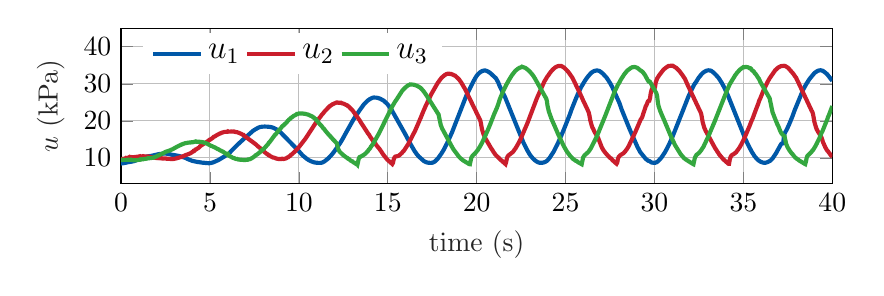
\begin{tikzpicture}

\begin{axis}[%
width=0.745\textwidth,
height=0.163\textwidth,
at={(0\textwidth,0\textwidth)},
scale only axis,
xmin=0,
xmax=40,
xlabel style={font=\color{white!15!black}},
xlabel={time (s)},
ymin=3,
ymax=45,
ylabel style={font=\color{white!15!black}},
ylabel={$u$ (kPa)},
axis background/.style={fill=white},
xmajorgrids,
ymajorgrids,
legend style={at={(0.03,0.97)}, anchor=north west, legend columns=3, legend cell align=left, align=left, draw=white!15!black},
legend style={font=\fontsize{12}{11}\selectfont, /tikz/every even row/.append style={column sep=0.5cm}, draw=none}
]
\addplot [color=mycolor1, line width=1.5pt]
  table[row sep=crcr]{%
0	8.5026\\
0.0800800000000024	8.5187\\
0.160159999999998	8.6027\\
0.280279999999998	8.7057\\
0.400399999999998	8.8437\\
0.440440000000002	8.8864\\
0.48048	8.8951\\
0.560560000000002	8.9534\\
0.72072	9.1069\\
0.96096	9.5408\\
1.041	9.646\\
1.2412	10.034\\
1.2813	10.082\\
1.4014	10.273\\
1.4815	10.392\\
1.6817	10.546\\
1.7217	10.582\\
1.7618	10.601\\
1.8418	10.705\\
1.9219	10.795\\
2.0821	10.975\\
2.1622	11.045\\
2.3223	11.126\\
2.4024	11.164\\
2.4424	11.178\\
2.5225	11.176\\
2.5626	11.138\\
2.6026	11.121\\
2.6827	11.035\\
2.7628	10.965\\
2.8028	10.908\\
2.8428	10.876\\
2.8829	10.82\\
3.003	10.757\\
3.043	10.711\\
3.1231	10.655\\
3.2833	10.494\\
3.4034	10.325\\
3.5235	10.152\\
3.6436	9.9577\\
3.7237	9.7517\\
3.8438	9.4979\\
3.8839	9.4379\\
4.004	9.2073\\
4.2843	8.9195\\
4.4444	8.812\\
4.5646	8.7193\\
4.6046	8.6968\\
4.6446	8.7056\\
4.6847	8.6745\\
4.7247	8.6663\\
4.7648	8.626\\
4.8048	8.6159\\
4.8448	8.5817\\
4.965	8.5727\\
5.045	8.6211\\
5.1652	8.7671\\
5.2853	9.002\\
5.3654	9.1772\\
5.4855	9.445\\
5.8058	10.373\\
5.966	10.867\\
6.046	11.15\\
6.1261	11.476\\
6.2062	11.903\\
6.4064	12.848\\
6.5265	13.445\\
6.967	15.4\\
7.0871	15.88\\
7.4074	17.242\\
7.5275	17.628\\
7.6877	18.07\\
7.8078	18.322\\
7.8478	18.369\\
7.968	18.433\\
8.0881	18.468\\
8.1281	18.442\\
8.2082	18.441\\
8.2482	18.416\\
8.2883	18.412\\
8.4084	18.336\\
8.4885	18.248\\
8.5285	18.175\\
8.5686	18.133\\
8.6887	17.84\\
8.7688	17.616\\
8.8889	17.244\\
8.969	16.913\\
9.0891	16.323\\
9.2492	15.547\\
10.01	11.77\\
10.21	10.687\\
10.45	9.7312\\
10.571	9.3645\\
10.611	9.2839\\
10.691	9.0806\\
10.851	8.8052\\
10.891	8.783\\
10.931	8.7258\\
11.051	8.6771\\
11.091	8.6452\\
11.211	8.6466\\
11.291	8.7174\\
11.331	8.7764\\
11.451	9.0912\\
11.652	9.8599\\
11.852	10.882\\
11.972	11.605\\
12.332	14.058\\
12.452	15.032\\
12.653	16.799\\
13.053	20.214\\
13.173	21.132\\
13.413	22.82\\
13.654	24.423\\
13.854	25.403\\
13.974	25.816\\
14.014	25.939\\
14.054	26.015\\
14.134	26.214\\
14.174	26.275\\
14.214	26.293\\
14.254	26.29\\
14.294	26.269\\
14.334	26.271\\
14.374	26.249\\
14.454	26.167\\
14.535	26.033\\
14.575	25.975\\
14.775	25.441\\
14.975	24.538\\
15.095	23.822\\
15.215	22.967\\
15.976	16.479\\
16.296	13.598\\
16.496	11.942\\
16.617	11.1\\
16.737	10.411\\
17.017	9.2019\\
17.137	8.8746\\
17.217	8.769\\
17.257	8.7146\\
17.337	8.6893\\
17.377	8.6518\\
17.417	8.6472\\
17.497	8.7046\\
17.538	8.7491\\
17.618	8.9383\\
17.658	9.0642\\
17.818	9.8269\\
18.018	11.182\\
18.138	12.115\\
18.338	13.97\\
18.619	16.966\\
19.419	26.801\\
19.82	30.688\\
19.98	32.014\\
20.06	32.517\\
20.18	33.056\\
20.26	33.311\\
20.34	33.503\\
20.38	33.536\\
20.42	33.589\\
20.46	33.62\\
20.541	33.515\\
20.621	33.35\\
20.701	33.119\\
20.781	32.834\\
20.901	32.306\\
21.021	31.739\\
21.061	31.607\\
21.101	31.369\\
21.221	30.271\\
21.301	29.301\\
21.582	26.562\\
22.623	14.209\\
22.823	12.25\\
22.983	10.94\\
23.063	10.422\\
23.183	9.7614\\
23.303	9.2473\\
23.423	8.8771\\
23.463	8.7948\\
23.544	8.6849\\
23.624	8.6771\\
23.704	8.7052\\
23.784	8.7887\\
23.864	8.946\\
23.944	9.1857\\
23.984	9.3434\\
24.104	10.018\\
24.344	11.8\\
24.545	13.712\\
24.745	15.874\\
24.905	17.686\\
25.225	21.559\\
25.345	23.179\\
25.546	25.594\\
25.666	26.966\\
25.866	29.042\\
26.106	30.961\\
26.266	32.007\\
26.386	32.674\\
26.466	33.043\\
26.547	33.307\\
26.627	33.488\\
26.667	33.529\\
26.707	33.552\\
26.747	33.608\\
26.827	33.563\\
26.867	33.517\\
26.907	33.442\\
26.947	33.339\\
27.107	32.696\\
27.307	31.652\\
27.508	30.165\\
27.628	29.105\\
28.028	24.81\\
28.148	23.132\\
28.589	17.903\\
29.029	13.101\\
29.189	11.642\\
29.269	11.141\\
29.349	10.676\\
29.469	9.9676\\
29.51	9.7362\\
29.59	9.4367\\
29.63	9.2747\\
29.67	9.1925\\
29.71	9.1578\\
29.83	8.7762\\
29.87	8.7286\\
29.91	8.7045\\
30.03	8.6725\\
30.07	8.7608\\
30.11	8.8093\\
30.19	9.0551\\
30.39	10.082\\
30.591	11.544\\
30.751	12.967\\
30.871	14.173\\
31.031	15.922\\
31.552	22.213\\
31.912	26.605\\
32.192	29.427\\
32.272	30.092\\
32.312	30.28\\
32.472	31.551\\
32.633	32.515\\
32.713	32.904\\
32.793	33.211\\
32.913	33.516\\
32.993	33.615\\
33.033	33.639\\
33.153	33.564\\
33.193	33.477\\
33.273	33.218\\
33.393	32.708\\
33.594	31.664\\
33.794	30.181\\
33.954	28.7\\
34.154	26.588\\
35.115	15.05\\
35.315	13.072\\
35.475	11.619\\
35.636	10.417\\
35.756	9.7389\\
35.836	9.3713\\
35.956	8.993\\
36.076	8.7643\\
36.116	8.7153\\
36.196	8.6835\\
36.236	8.6976\\
36.276	8.7342\\
36.316	8.7886\\
36.436	9.0409\\
36.517	9.2619\\
36.637	9.8381\\
36.837	11.278\\
37.117	13.713\\
37.157	13.863\\
37.197	13.92\\
37.237	13.952\\
37.277	15.634\\
37.317	16.54\\
37.357	16.974\\
37.437	17.638\\
37.558	18.897\\
37.758	21.201\\
37.878	22.801\\
38.358	28.381\\
38.519	29.806\\
38.719	31.302\\
38.999	32.929\\
39.159	33.446\\
39.199	33.533\\
39.239	33.588\\
39.319	33.642\\
39.359	33.641\\
39.399	33.588\\
39.439	33.559\\
39.479	33.471\\
39.64	32.879\\
39.72	32.524\\
40	30.798\\
};
\addlegendentry{$u_1$}

\addplot [color=mycolor2, line width=1.5pt]
  table[row sep=crcr]{%
0	9.6339\\
0.0400399999999976	9.6465\\
0.0800800000000024	9.7443\\
0.12012	9.7155\\
0.160159999999998	9.7762\\
0.200200000000002	9.8106\\
0.24024	9.8811\\
0.280279999999998	10.018\\
0.320320000000002	9.9697\\
0.36036	10.024\\
0.400399999999998	10.05\\
0.440440000000002	10.101\\
0.48048	10.247\\
0.520519999999998	10.129\\
0.560560000000002	10.23\\
0.6006	10.162\\
0.680680000000002	10.174\\
0.72072	10.21\\
0.760759999999998	10.221\\
0.800800000000002	10.265\\
0.84084	10.27\\
1.001	10.378\\
1.041	10.381\\
1.0811	10.464\\
1.1211	10.4\\
1.1612	10.418\\
1.2012	10.416\\
1.2412	10.483\\
1.2813	10.436\\
1.4014	10.399\\
1.4414	10.4\\
1.4815	10.385\\
1.5215	10.413\\
1.5616	10.325\\
1.6016	10.31\\
1.6416	10.231\\
1.6817	10.212\\
1.7217	10.16\\
1.7618	10.148\\
1.8018	10.07\\
1.8418	10.061\\
1.8819	10.066\\
1.9219	10.037\\
1.962	9.9915\\
2.002	9.9683\\
2.042	9.966\\
2.0821	9.9237\\
2.1221	9.9382\\
2.1622	9.9364\\
2.2022	9.9018\\
2.2422	9.893\\
2.2823	9.9238\\
2.3223	9.8414\\
2.4024	9.8356\\
2.4424	9.8738\\
2.4825	9.8519\\
2.5225	9.8445\\
2.5626	9.785\\
2.6426	9.7665\\
2.6827	9.7303\\
2.7227	9.7348\\
2.8028	9.7011\\
2.8428	9.7053\\
2.8829	9.6952\\
2.9229	9.7403\\
2.963	9.7195\\
3.043	9.8195\\
3.0831	9.8332\\
3.3634	10.228\\
3.4034	10.336\\
3.4434	10.359\\
3.5636	10.588\\
3.6036	10.712\\
3.6436	10.758\\
3.6837	10.864\\
3.7237	10.901\\
3.8038	11.05\\
3.8839	11.206\\
3.964	11.423\\
4.004	11.599\\
4.044	11.671\\
4.0841	11.92\\
4.1241	11.933\\
4.2042	12.299\\
4.2442	12.354\\
4.3243	12.639\\
4.3644	12.726\\
4.4044	12.89\\
4.4444	13.14\\
4.5646	13.519\\
4.7247	14.049\\
4.8048	14.295\\
4.9249	14.656\\
4.965	14.873\\
5.005	14.905\\
5.0851	15.173\\
5.1652	15.444\\
5.2052	15.667\\
5.2452	15.723\\
5.3253	15.967\\
5.4054	16.198\\
5.5656	16.607\\
5.6056	16.654\\
5.6456	16.761\\
5.8058	17.005\\
5.966	17.065\\
6.006	17.176\\
6.046	17.081\\
6.1662	17.105\\
6.2062	17.149\\
6.2462	17.106\\
6.2863	17.103\\
6.3263	17.116\\
6.3664	17.11\\
6.4064	17.012\\
6.4464	16.998\\
6.4865	16.949\\
6.5265	16.939\\
6.6466	16.721\\
6.7668	16.475\\
6.8468	16.246\\
6.8869	16.221\\
6.9269	15.976\\
7.5676	13.705\\
7.6476	13.349\\
7.7277	13.004\\
7.9279	12.244\\
7.968	12.007\\
8.008	11.9\\
8.048	11.666\\
8.2082	11.046\\
8.2482	10.971\\
8.2883	10.777\\
8.3283	10.718\\
8.3684	10.542\\
8.4885	10.237\\
8.5686	10.063\\
8.6086	10.061\\
8.6486	10.009\\
8.7287	9.8253\\
8.8488	9.7222\\
8.8889	9.7098\\
8.9289	9.7262\\
8.969	9.6856\\
9.009	9.6801\\
9.049	9.7711\\
9.0891	9.7705\\
9.1291	9.7033\\
9.1692	9.7304\\
9.2492	9.8299\\
9.2893	9.8942\\
9.3293	10.007\\
9.3694	10.162\\
9.4094	10.192\\
9.4494	10.405\\
9.4895	10.484\\
9.5295	10.636\\
9.5696	10.883\\
9.6096	10.973\\
9.7698	11.691\\
9.8899	12.351\\
9.9299	12.469\\
10.37	15.18\\
11.051	20.179\\
11.171	20.877\\
11.251	21.345\\
11.291	21.668\\
11.331	21.831\\
11.451	22.553\\
11.732	23.959\\
11.772	24.055\\
11.812	24.221\\
11.852	24.326\\
11.892	24.476\\
12.132	24.972\\
12.172	24.953\\
12.212	24.892\\
12.252	24.899\\
12.292	24.85\\
12.332	24.898\\
12.372	24.905\\
12.412	24.752\\
12.492	24.663\\
12.573	24.508\\
12.733	24.136\\
12.773	23.926\\
12.813	23.852\\
12.893	23.413\\
13.013	22.873\\
13.413	20.182\\
13.493	19.514\\
13.574	18.942\\
13.894	16.571\\
13.934	16.368\\
14.014	15.707\\
14.174	14.607\\
14.254	14.093\\
14.294	13.962\\
14.334	13.576\\
14.535	12.423\\
14.655	11.585\\
14.735	10.97\\
14.975	9.5249\\
15.215	8.5171\\
15.255	8.3469\\
15.295	8.6929\\
15.335	9.6258\\
15.375	10.093\\
15.415	10.305\\
15.455	10.42\\
15.495	10.428\\
15.576	10.518\\
15.616	10.595\\
15.656	10.725\\
15.816	11.433\\
15.856	11.735\\
15.896	11.864\\
16.136	13.607\\
16.537	17.322\\
16.857	20.88\\
16.977	22.303\\
17.137	24.076\\
17.457	27.283\\
17.778	29.985\\
17.898	30.835\\
17.978	31.322\\
18.018	31.597\\
18.098	31.93\\
18.178	32.251\\
18.218	32.397\\
18.258	32.489\\
18.298	32.621\\
18.338	32.691\\
18.378	32.702\\
18.418	32.745\\
18.458	32.723\\
18.498	32.667\\
18.539	32.685\\
18.579	32.601\\
18.619	32.553\\
18.739	32.266\\
18.779	32.216\\
18.939	31.528\\
19.019	31.125\\
19.139	30.291\\
19.339	28.648\\
20.1	21.136\\
20.18	20.395\\
20.22	19.832\\
20.3	17.715\\
20.38	16.448\\
20.501	15.184\\
20.821	12.533\\
20.861	12.302\\
20.941	11.653\\
21.061	10.838\\
21.181	10.26\\
21.221	10.119\\
21.301	9.6957\\
21.381	9.3552\\
21.421	9.2059\\
21.502	8.8388\\
21.622	8.3338\\
21.662	8.9686\\
21.702	9.9294\\
21.742	10.402\\
21.782	10.647\\
22.022	11.531\\
22.102	12.006\\
22.142	12.354\\
22.182	12.541\\
22.382	14.204\\
22.462	15.003\\
22.863	19.482\\
23.383	26.062\\
23.824	30.797\\
23.864	31.039\\
23.984	32.042\\
24.024	32.241\\
24.144	33.092\\
24.264	33.765\\
24.384	34.301\\
24.464	34.557\\
24.545	34.728\\
24.625	34.818\\
24.665	34.83\\
24.705	34.81\\
24.745	34.821\\
24.785	34.744\\
24.905	34.409\\
25.065	33.662\\
25.145	33.243\\
25.225	32.733\\
25.385	31.607\\
25.465	30.847\\
25.786	27.656\\
25.986	25.531\\
26.226	23.102\\
26.306	22.211\\
26.346	21.346\\
26.386	20.201\\
26.466	18.799\\
26.507	18.223\\
26.547	17.891\\
26.627	17.029\\
26.707	16.38\\
26.827	15.444\\
27.027	12.96\\
27.107	12.221\\
27.227	11.428\\
27.387	10.564\\
27.427	10.418\\
27.467	10.147\\
27.508	9.9792\\
27.548	9.9077\\
27.628	9.4412\\
27.748	8.9097\\
27.828	8.5833\\
27.868	8.4312\\
27.908	8.8027\\
27.948	9.8291\\
27.988	10.26\\
28.068	10.701\\
28.268	11.302\\
28.308	11.558\\
28.348	11.732\\
28.468	12.524\\
28.549	13.185\\
28.909	16.824\\
29.229	20.412\\
29.269	20.658\\
29.309	20.987\\
29.389	22.243\\
29.429	22.744\\
29.51	23.953\\
29.55	24.253\\
29.63	25.257\\
29.67	25.446\\
29.71	25.462\\
29.75	26.131\\
29.79	27.498\\
29.83	28.266\\
29.87	28.723\\
29.91	28.761\\
29.95	28.668\\
29.99	28.626\\
30.03	29.109\\
30.07	30.368\\
30.15	31.441\\
30.27	32.355\\
30.39	33.094\\
30.511	33.839\\
30.591	34.152\\
30.671	34.45\\
30.791	34.817\\
30.831	34.814\\
30.871	34.85\\
30.951	34.861\\
31.031	34.857\\
31.191	34.393\\
31.231	34.269\\
31.311	33.873\\
31.391	33.511\\
31.471	33.002\\
31.592	32.213\\
31.712	31.355\\
31.832	30.036\\
31.952	28.807\\
32.553	22.695\\
32.593	22.335\\
32.633	21.76\\
32.713	19.609\\
32.793	18.238\\
32.873	17.369\\
33.393	12.776\\
33.554	11.573\\
33.594	11.325\\
33.634	10.963\\
33.874	9.6096\\
33.994	9.1169\\
34.074	8.7617\\
34.154	8.4364\\
34.194	8.4368\\
34.234	9.5054\\
34.274	10.209\\
34.314	10.551\\
34.354	10.761\\
34.394	10.886\\
34.434	10.96\\
34.515	11.217\\
34.555	11.428\\
34.595	11.557\\
34.795	12.877\\
34.955	14.321\\
35.075	15.551\\
35.355	18.714\\
35.435	19.726\\
35.516	20.585\\
35.716	23.184\\
35.836	24.648\\
35.876	25.306\\
35.956	26.14\\
36.156	28.511\\
36.236	29.274\\
36.356	30.474\\
36.476	31.496\\
36.797	33.71\\
36.837	33.84\\
36.957	34.401\\
37.117	34.764\\
37.197	34.834\\
37.237	34.821\\
37.277	34.861\\
37.357	34.785\\
37.518	34.293\\
37.798	32.754\\
37.918	31.904\\
37.958	31.682\\
38.158	29.665\\
38.839	22.725\\
38.879	22.391\\
38.919	21.754\\
38.999	19.589\\
39.079	18.329\\
39.119	17.745\\
39.199	17.05\\
39.359	15.858\\
39.399	15.404\\
39.479	14.235\\
39.6	12.922\\
39.68	12.22\\
39.72	11.954\\
39.76	11.796\\
39.8	11.445\\
39.84	11.254\\
39.92	10.7\\
40	10.317\\
};
\addlegendentry{$u_2$}

\addplot [color=mycolor3, line width=1.5pt]
  table[row sep=crcr]{%
0	9.429\\
0.0400399999999976	9.4292\\
0.0800800000000024	9.487\\
0.12012	9.4466\\
0.160159999999998	9.4812\\
0.280279999999998	9.4644\\
0.36036	9.5017\\
0.520519999999998	9.4733\\
0.560560000000002	9.5235\\
0.6006	9.4091\\
0.680680000000002	9.3907\\
0.72072	9.3606\\
0.800800000000002	9.3536\\
0.84084	9.3812\\
0.880879999999998	9.3891\\
0.920920000000002	9.4365\\
0.96096	9.4465\\
1.001	9.4784\\
1.041	9.494\\
1.0811	9.6124\\
1.1211	9.5486\\
1.1612	9.6075\\
1.2012	9.6362\\
1.2412	9.6249\\
1.3213	9.7386\\
1.3614	9.7272\\
1.4815	9.8425\\
1.5215	9.9468\\
1.5616	9.8829\\
1.6416	9.9488\\
1.6817	9.9525\\
1.8018	10.06\\
1.8418	10.097\\
1.8819	10.234\\
1.9219	10.257\\
1.962	10.381\\
2.002	10.424\\
2.042	10.551\\
2.0821	10.617\\
2.1221	10.731\\
2.1622	10.793\\
2.2022	10.915\\
2.2422	10.983\\
2.2823	11.099\\
2.3223	11.153\\
2.4024	11.34\\
2.4825	11.585\\
2.5225	11.675\\
2.5626	11.721\\
2.6026	11.794\\
2.6426	11.838\\
2.8028	12.141\\
2.8829	12.317\\
2.9229	12.397\\
3.003	12.636\\
3.043	12.725\\
3.1231	12.946\\
3.4434	13.7\\
3.4835	13.748\\
3.5235	13.834\\
3.5636	13.89\\
3.6036	13.969\\
3.6436	13.994\\
3.6837	14.044\\
3.7237	14.061\\
3.8038	14.132\\
3.9239	14.168\\
3.964	14.226\\
4.044	14.24\\
4.1241	14.326\\
4.2042	14.451\\
4.2442	14.356\\
4.4044	14.362\\
4.4845	14.309\\
4.5245	14.324\\
4.5646	14.24\\
4.6046	14.23\\
4.6446	14.184\\
4.6847	14.099\\
4.7247	14.064\\
4.8048	13.894\\
4.8448	13.822\\
4.965	13.498\\
5.005	13.429\\
5.0851	13.196\\
5.1251	13.163\\
5.1652	13.077\\
5.2052	12.96\\
5.2452	12.904\\
5.4454	12.367\\
5.4855	12.314\\
5.5656	12.047\\
5.6456	11.893\\
5.6857	11.754\\
5.7257	11.695\\
5.8058	11.431\\
5.8458	11.343\\
5.8859	11.17\\
5.9259	11.108\\
5.966	10.944\\
6.006	11.046\\
6.046	10.659\\
6.1261	10.467\\
6.1662	10.332\\
6.2062	10.252\\
6.2462	10.123\\
6.3263	9.9611\\
6.3664	9.9404\\
6.4064	9.8107\\
6.4865	9.6867\\
6.5265	9.7255\\
6.6066	9.535\\
6.6466	9.5535\\
6.6867	9.5157\\
6.7267	9.5036\\
6.7668	9.5106\\
6.8068	9.4711\\
6.8468	9.4682\\
6.8869	9.4287\\
6.9269	9.4547\\
6.967	9.4111\\
7.007	9.463\\
7.1271	9.4988\\
7.1672	9.6155\\
7.2072	9.6039\\
7.2472	9.6641\\
7.3273	9.8581\\
7.4074	10.074\\
7.5275	10.484\\
7.5676	10.714\\
7.6076	10.784\\
7.6476	10.942\\
7.6877	11.048\\
7.8478	11.7\\
7.8879	11.962\\
7.968	12.198\\
8.008	12.443\\
8.048	12.548\\
8.2883	13.843\\
8.3283	14.182\\
8.3684	14.341\\
8.6086	15.901\\
8.6486	16.184\\
8.6887	16.313\\
8.7688	16.806\\
8.8088	17.022\\
8.8488	17.331\\
9.009	18.151\\
9.049	18.447\\
9.0891	18.632\\
9.1291	18.729\\
9.2092	19.11\\
9.3293	19.685\\
9.3694	19.99\\
9.4094	20.121\\
9.4494	20.366\\
9.4895	20.46\\
9.5696	20.871\\
9.6096	20.946\\
9.6897	21.267\\
9.8498	21.686\\
9.8899	21.857\\
9.9299	21.844\\
10.01	22.006\\
10.05	21.984\\
10.09	22.002\\
10.17	21.999\\
10.21	22.004\\
10.29	21.911\\
10.33	21.924\\
10.45	21.764\\
10.531	21.688\\
10.611	21.487\\
10.771	21.134\\
10.811	20.916\\
10.851	20.868\\
10.891	20.606\\
10.931	20.536\\
11.171	19.155\\
11.291	18.549\\
11.371	18.007\\
11.411	17.879\\
11.491	17.337\\
11.692	16.199\\
11.732	16.061\\
11.772	15.771\\
11.812	15.608\\
11.932	14.933\\
12.012	14.557\\
12.132	13.941\\
12.212	12.457\\
12.292	11.678\\
12.492	10.777\\
12.693	10.044\\
12.733	9.9786\\
12.773	9.7627\\
12.813	9.7175\\
12.893	9.3668\\
12.933	9.2171\\
13.013	9.0673\\
13.053	8.8597\\
13.093	8.7396\\
13.133	8.6915\\
13.213	8.3754\\
13.253	8.4056\\
13.293	8.1874\\
13.373	9.8582\\
13.413	10.203\\
13.453	10.262\\
13.493	10.404\\
13.534	10.479\\
13.654	10.84\\
13.734	11.111\\
13.894	11.922\\
13.934	12.247\\
13.974	12.402\\
14.014	12.655\\
14.054	13.04\\
14.094	13.237\\
14.214	14.127\\
14.494	16.525\\
15.255	23.912\\
15.415	25.208\\
15.495	25.747\\
15.776	27.844\\
15.816	28.135\\
15.896	28.547\\
15.976	28.941\\
16.096	29.415\\
16.176	29.659\\
16.216	29.718\\
16.256	29.829\\
16.296	29.784\\
16.336	29.819\\
16.376	29.788\\
16.416	29.781\\
16.496	29.716\\
16.577	29.562\\
16.617	29.52\\
16.697	29.324\\
16.737	29.244\\
16.777	29.085\\
16.817	28.995\\
16.897	28.651\\
17.017	27.973\\
17.137	27.175\\
17.858	21.719\\
17.978	18.927\\
18.058	17.923\\
18.138	17.229\\
18.619	12.931\\
18.699	12.275\\
19.019	10.24\\
19.099	9.8676\\
19.219	9.3894\\
19.379	8.9102\\
19.419	8.7718\\
19.459	8.6817\\
19.58	8.3176\\
19.62	8.2897\\
19.7	10.06\\
19.78	10.658\\
19.82	10.857\\
19.86	10.99\\
19.94	11.398\\
20.06	12.111\\
20.18	13.024\\
20.3	14.044\\
20.46	15.716\\
20.621	17.451\\
20.781	19.307\\
20.981	21.789\\
21.141	23.542\\
21.221	24.606\\
21.301	25.834\\
21.461	27.698\\
21.662	29.704\\
21.822	31.065\\
21.982	32.32\\
22.142	33.306\\
22.182	33.54\\
22.342	34.15\\
22.382	34.238\\
22.422	34.361\\
22.503	34.457\\
22.543	34.608\\
22.583	34.507\\
22.623	34.486\\
22.743	34.271\\
22.863	33.84\\
22.983	33.326\\
23.143	32.428\\
23.263	31.555\\
23.864	26.414\\
23.904	26.098\\
23.944	25.502\\
23.984	24.095\\
24.064	22.443\\
24.224	20.328\\
24.424	18.172\\
24.585	16.353\\
24.905	13.132\\
25.065	11.791\\
25.265	10.503\\
25.425	9.7089\\
25.586	9.1833\\
25.626	9.1335\\
25.706	8.8332\\
25.746	8.6985\\
25.786	8.6198\\
25.906	8.2961\\
25.986	10.07\\
26.026	10.443\\
26.066	10.691\\
26.266	11.549\\
26.346	12.049\\
26.426	12.617\\
26.747	15.681\\
27.227	21.319\\
27.788	28.259\\
27.828	28.56\\
27.948	29.807\\
28.028	30.375\\
28.108	31.129\\
28.308	32.621\\
28.468	33.547\\
28.669	34.288\\
28.749	34.462\\
28.789	34.477\\
28.829	34.525\\
28.869	34.545\\
28.909	34.516\\
28.989	34.394\\
29.029	34.327\\
29.229	33.547\\
29.269	33.454\\
29.349	33.129\\
29.469	32.334\\
29.63	30.906\\
29.67	30.632\\
29.71	30.651\\
29.75	30.515\\
30.11	27.41\\
30.15	26.604\\
30.19	24.974\\
30.23	23.989\\
30.31	22.805\\
30.43	21.42\\
30.551	20.103\\
30.911	15.983\\
31.151	13.495\\
31.471	10.996\\
31.552	10.555\\
31.672	9.8877\\
31.712	9.7935\\
31.752	9.6011\\
32.032	8.7526\\
32.072	8.6903\\
32.112	8.5057\\
32.192	8.3089\\
32.272	10.039\\
32.352	10.757\\
32.392	10.943\\
32.432	11.048\\
32.472	11.254\\
32.513	11.383\\
32.633	12.118\\
32.713	12.717\\
32.753	13.002\\
33.033	15.857\\
33.393	19.922\\
34.074	28.196\\
34.234	29.896\\
34.555	32.434\\
34.595	32.616\\
34.635	32.932\\
34.715	33.353\\
34.795	33.792\\
34.995	34.503\\
35.035	34.448\\
35.115	34.536\\
35.155	34.532\\
35.195	34.512\\
35.235	34.478\\
35.315	34.343\\
35.355	34.186\\
35.395	34.189\\
35.435	34.038\\
35.475	33.709\\
35.516	33.534\\
35.556	33.432\\
35.596	33.225\\
35.636	32.883\\
35.676	32.725\\
35.716	32.488\\
35.796	31.881\\
35.836	31.552\\
35.876	31.347\\
35.956	30.484\\
36.476	26.09\\
36.637	22.377\\
36.757	20.861\\
36.837	19.918\\
36.917	18.979\\
36.957	18.653\\
37.077	17.189\\
37.157	16.514\\
37.277	15.959\\
37.317	15.799\\
37.397	13.921\\
37.477	12.945\\
37.598	11.981\\
37.718	11.223\\
37.758	11.038\\
37.918	10.067\\
37.958	9.9624\\
38.038	9.635\\
38.078	9.553\\
38.118	9.3611\\
38.278	8.8824\\
38.318	8.7954\\
38.398	8.5391\\
38.478	8.3289\\
38.519	9.0558\\
38.559	10.048\\
38.599	10.543\\
38.839	11.657\\
38.879	12.012\\
38.919	12.126\\
39.039	13.088\\
39.119	13.795\\
39.279	15.37\\
39.399	16.834\\
39.439	17.127\\
39.64	19.511\\
39.72	20.437\\
39.76	21.062\\
39.8	21.436\\
39.88	22.465\\
40	23.999\\
};
\addlegendentry{$u_3$}

\end{axis}
\end{tikzpicture}%
   \vspace{-0.25cm}
   \caption{ Spatial representation of the nonlinear stiffness, \ie,  elongation stiffness (left) and bending stiffness (right) for a radially distributed sampling of the curvature joint space $(\kappa_x,\,\kappa_y) \in [-\pi,\pi)$. The experimental data is shown in (\ldata{lightgray}). Again, note that the bending stiffness has a discrete symmetry in the circumferential direction with periodicity of $\tfrac{2\pi}{3}$.}
   \vspace{-0.1cm}
   \label{fig:C2:openloop_2D}
 \end{figure}

Second, we consider a forced scenario in which a regulated pressure input is applied to the pneumatic bellows, \ie, $\uB \neq \vec{0}_3$. Since the pneumatic mapping $\mat{G}$ in \eqref{eq:C2:mapping_H} plays an important role here, the actuator coefficients are recomputed to match the experimental data better. To be more specific, by considering a pre-defined set of excitation signals $u(t)$ of various amplitudes and frequencies, a least-squares optimization routine is employed that minimizes the difference between the measured states $\hat{q}$ with the simulated states ${q}$ by tuning the coefficients $\alpha_\varepsilon$ and $\alpha_\kappa$. This leads to the following values: $\alpha_\varepsilon = 2.34\cdot 10^{-7}$ and $\alpha_\kappa =  1.61\cdot 10^{-8}$. As for the excitation signal, we have chosen the following input:
%
\begin{equation}
u_i(t) = P_0 + P_A \left(\frac{1}{2} + \frac{1}{2}\sin(t + \phi_i) \right)\cdot \max(0.05t,1),
\end{equation}
%
with a static offset $P_0 = 10$ kPa, an amplitude $P_A = 25$ kPa, and a phase offset $\phi_i = (i-1)\frac{2\pi}{m}$ rad. To highlight the significance of the proposed hyper-elastic modeling approach, we also compare the results using an optimized Hookean material material model with $k_e = 50.6$ N/m and $k_b = 5.8\cdot 10^{-4}$ Nm/rad. The initial conditions are set to zero. The validations results for both the FEM-driven hyper-elasticity model and linear model in the forced setting are shown in Figure \ref{fig:C2:openloop_2D}. The figure also shows the measured outputs from the pneumatic VEAB regulators $u_i(t)$, which are directly fed into both linear and hyper-elastic models. 

Given these results, two key observations can be made. First, both the linear Hookean and hyper-elastic models provide reasonable accuracy for small deformations $0 \le \kappa(t) \le 3$ with a RMS error of $\pm0.13$ and $\pm0.16$ in curvature, respectively. However, as deformations exceed the linear regime, the hyper-elastic model significantly outperforms the Hookean model. Focusing on the hyper-elastic model, both the asymmetric stiffness in radial direction and the strain-hardening are captured well, where the the linear models is not sufficiently rich to capture the material effects. The overall RMS errors for the linear and hyper-elastic model are $\pm1.79$ and $\pm0.21$ in curvature, respectively. Regarding the end-effector accuracy, the overall RMS errors for the linear and hyper-elastic model are $\pm2.58$ and $\pm0.65$ mm, respectively; which translates to an arc-length normalized error of $\pm4.09\%$ and $\pm1.03\%$. These  numerical comparison  results show that introducing nonlinear elastic effects driven by FEM-data can further improve the accuracy for a larger region of the soft robot's workspace.

For the last validation case, we subject the soft robot to an external payload of mass $\delta_m$ located at the end-effector. To model the disturbance, we use the expression for the external payload disturbance model $\delta_m$ in \eqref{eq:C2:delta_payload}. The goal here is \textit{a)} to demonstrate the accuracy of the proposed payload model and quasi-static behavior of the dynamic model, and \textit{b)} to highlight the limitations of the PCC assumptions under certain conditions. In this analysis, we consider three different payloads $m_\delta = \{0, 50,\,100,\,150\}$ \si{\gram}. The experimental results of the payloads deformations and the resulting quasi-static deformations of the dynamic model are shown in Figure \ref{fig:C2:compare_deflect}. 
%The associated code for the external payload simulations can be found under \texttt{./valid\_one\_link\_tipload.m}.

%
\begin{figure}[!t]
  %\vspace{-2mm}
  \centering
  \includegraphics*{./pdf/thesis-figure-4-18.pdf}
  %% This file was created by matlab2tikz.
%
\begin{tikzpicture}

\begin{axis}[%
width=0.192\textwidth,
height=0.202\textwidth,
at={(0.012\textwidth,0.183\textwidth)},
scale only axis,
axis on top,
xmin=0.5,
xmax=728.5,
tick align=outside,
y dir=reverse,
ymin=0.5,
ymax=728.5,
axis line style={draw=none},
ticks=none,
ylabel style={yshift=-3.5pt}
]
\addplot [forget plot] graphics [xmin=0.5, xmax=728.5, ymin=0.5, ymax=728.5] {fig_C2_compare_deflect-1.png};
\end{axis}

\begin{axis}[%
width=0.192\textwidth,
height=0.202\textwidth,
at={(0.257\textwidth,0.183\textwidth)},
scale only axis,
axis on top,
xmin=0.5,
xmax=728.5,
tick align=outside,
y dir=reverse,
ymin=0.5,
ymax=728.5,
axis line style={draw=none},
ticks=none,
ylabel style={yshift=-3.5pt}
]
\addplot [forget plot] graphics [xmin=0.5, xmax=728.5, ymin=0.5, ymax=728.5] {fig_C2_compare_deflect-2.png};
\end{axis}

\begin{axis}[%
width=0.192\textwidth,
height=0.202\textwidth,
at={(0.501\textwidth,0.183\textwidth)},
scale only axis,
axis on top,
xmin=0.5,
xmax=728.5,
tick align=outside,
y dir=reverse,
ymin=0.5,
ymax=728.5,
axis line style={draw=none},
ticks=none,
ylabel style={yshift=-3.5pt}
]
\addplot [forget plot] graphics [xmin=0.5, xmax=728.5, ymin=0.5, ymax=728.5] {fig_C2_compare_deflect-3.png};
\end{axis}

\begin{axis}[%
width=0.192\textwidth,
height=0.202\textwidth,
at={(0.746\textwidth,0.183\textwidth)},
scale only axis,
axis on top,
xmin=0.5,
xmax=728.5,
tick align=outside,
y dir=reverse,
ymin=0.5,
ymax=728.5,
axis line style={draw=none},
ticks=none,
ylabel style={yshift=-3.5pt}
]
\addplot [forget plot] graphics [xmin=0.5, xmax=728.5, ymin=0.5, ymax=728.5] {fig_C2_compare_deflect-4.png};
\end{axis}

\begin{axis}[%
width=0.216\textwidth,
height=0.156\textwidth,
at={(0\textwidth,0\textwidth)},
scale only axis,
axis on top,
xmin=0.5,
xmax=522.5,
tick align=outside,
y dir=reverse,
ymin=0.5,
ymax=358.5,
axis line style={draw=none},
ticks=none,
ylabel style={yshift=-3.5pt}
]
\addplot [forget plot] graphics [xmin=0.5, xmax=522.5, ymin=0.5, ymax=358.5] {fig_C2_compare_deflect-5.png};
\end{axis}

\begin{axis}[%
width=0.216\textwidth,
height=0.156\textwidth,
at={(0.245\textwidth,0\textwidth)},
scale only axis,
axis on top,
xmin=0.5,
xmax=522.5,
tick align=outside,
y dir=reverse,
ymin=0.5,
ymax=358.5,
axis line style={draw=none},
ticks=none,
ylabel style={yshift=-3.5pt}
]
\addplot [forget plot] graphics [xmin=0.5, xmax=522.5, ymin=0.5, ymax=358.5] {fig_C2_compare_deflect-6.png};
\end{axis}

\begin{axis}[%
width=0.216\textwidth,
height=0.156\textwidth,
at={(0.49\textwidth,0\textwidth)},
scale only axis,
axis on top,
xmin=0.5,
xmax=522.5,
tick align=outside,
y dir=reverse,
ymin=0.5,
ymax=358.5,
axis line style={draw=none},
ticks=none,
ylabel style={yshift=-3.5pt}
]
\addplot [forget plot] graphics [xmin=0.5, xmax=522.5, ymin=0.5, ymax=358.5] {fig_C2_compare_deflect-7.png};
\end{axis}

\begin{axis}[%
width=0.216\textwidth,
height=0.156\textwidth,
at={(0.734\textwidth,0\textwidth)},
scale only axis,
axis on top,
xmin=0.5,
xmax=522.5,
tick align=outside,
y dir=reverse,
ymin=0.5,
ymax=358.5,
axis line style={draw=none},
ticks=none,
ylabel style={yshift=-3.5pt}
]
\addplot [forget plot] graphics [xmin=0.5, xmax=522.5, ymin=0.5, ymax=358.5] {fig_C2_compare_deflect-8.png};
\end{axis}

\begin{axis}[%
width=0.969\textwidth,
height=0.459\textwidth,
at={(-0.01\textwidth,-0.069\textwidth)},
scale only axis,
xmin=0,
xmax=1,
ymin=0,
ymax=1,
axis line style={draw=none},
ticks=none,
axis x line*=bottom,
axis y line*=left,
ylabel style={yshift=-3.5pt}
]
\end{axis}
\end{tikzpicture}%
  \vspace{-5mm}
  \caption{Experimental validation of the one-link soft robot subjected to various end-effector payloads of different mass $m_\delta = \{0,50,100,150\}$ \si{\gram}. The deformed 3D-model in (\textcolor{PurpleLight}{$\bullet$}) corresponds to the estimated joint configuration based on the measurements from the IMU and depth camera, where the optimal marker location is shown in (\textcolor{lightgreen}{$\bullet$}) .}
  \label{fig:C2:compare_deflect}
\end{figure}
%

As can be seen, the quasi-static behavior of the dynamic model matches the experimental results relatively well for smaller payloads. For the mass $m_\delta = 0.05$ kg, the Euclidean error between the model and the measurement are $\pm1.31$ mm. Increasing the payload to $m_\delta = 0.1$ kg leads to an error of $\pm2.15$ mm. We can also clearly observe that the estimate of the backbone curve subject to the PCC condition is beginning to deviate from the ground truth yet the overall shape still matches the experimental data. Lastly, by further increase the payload $m_\delta = 0.15$ kg, we clearly observe the limitations of the PCC condition under external loads -- with an end-effector error of $3.98$ mm. Also, there is a clear discrepancy in the backbone curve of the model and the ground truth, which might imply the PCC condition is no longer valid here as the payload could induce non-constant curvatures along the backbone. A possible solution might be to introduce a different shape parametrization, similar to the works \cite{Chirikjian1994,Boyer2021,Renda2020,DellaSantina2020}.

\textbf{Model benchmark -- Multi-link soft manipulator case}:
\noindent In this section, we benchmark the proposed numerical integration scheme for a dynamic model of a six-link soft robot manipulator ($N = 6$). Here, we want to highlight that sufficient numerical speed can be obtained while preserving sufficient numerical precision. This is an important criteria for model-based control, as slow numerical models lack transferability from theory to application. As mentioned earlier, the numerical integration of the Lagrangian entities is the computational bottleneck. Although the MDE solver does aid with numerical performance; ultimately, using a balanced spatial and temporal discretization impacts real-time performance the most. Trivially, using larger stepsize -- both in space and time -- lead to a decrease in numerical precision; and in some cases numerical instability. In this benchmark, we investigate these effects by varying two solver parameters: the spatial stepsize of the explicit MDE solver denoted by $\Delta \sigma$ and the temporal stepsize of the implicit trapezoidal solver denoted by $\Delta t$. For convenience, we represent these stepsizes as standardized parameters: the number of finite elements $N_s = L/\Delta \sigma$ and the implicit solver frequency $f_s = \Delta t\inv$. For the benchmark, we choose a total length of $L = 0.15$ m and simulation time of $T = 10$ s.

%
The extension to the multi-link soft robot ($N = 6$) can be described by a following generalized coordinates with the following structure:
%
\begin{equation}
\q = \left(\,\varepsilon_1,\,\kappa_{x,1},\kappa_{y,1},...,\varepsilon_6,\,\kappa_{x,6},\kappa_{y,6} \, \right)^\top \in \mathcal{Q}
\end{equation}
%
To ensure the soft manipulator is self-supporting, we introduce slight variations to the hyper-elastic stiffness, link lengths, and the inertial properties of the dynamical system. Considering homogeneity, all links are chosen identical in length and mass: intrinsic link length $L_i = 0.025$ m and mass $m_i = 0.05$ kg. Next, the bending stiffness is slightly altered where we choose $\alpha_3 = 0.425$ Nm/rad and $\alpha_4 = 0.4$ Nm/rad. Please note that the material domain is now given by $\Xs = [0,\sum^N_{i=1} L_i]$. To introduce some interesting dynamics for the benchmark, we purely excite the first link of the serial-chain soft robot manipulator with a harmonic input:
%
\begin{align}
u_i(t) = \begin{cases}
P_a \cos(\pi t) & \text{for} \; i = 1, \\
0 & \text{otherwise},
\label{eq:harm_freq}
\end{cases}
\end{align}
%
where $P_a = 125$ kPa is the pressure amplitude. As for the pneumatic mapping that converts pressure to joint torques, we choose $\tauB = \left(\GB \otimes \mat{I}_6 \right)\uB $ as the corresponding pneumatic map for the six-link soft manipulator. In total 36 benchmark simulations with different solver settings were performed and tested for their precision relative to a high-precision model ($f_s = 500$ Hz and $N_s = 500$). The state trajectories of the high-precision model are shown in Figure \ref{fig:C2:multilink_states}, whereas Figure \ref{fig:C2:multilink_3d} is provided to highlight the underlying dynamics and the trajectory of the end-effector. The results for all benchmark simulations are shown in Table \ref{tab:benchmark_table}. %The associated code for the six-link simulations can be found under \texttt{./benchmark\_six\_link.m} on the repository.

Let us first discuss the dynamics of the six-link soft manipulator subjected to a harmonic input. Given this relatively straightforward harmonic excitation, some interesting (stable) nonlinear dynamics appear. Although we excite the system using one harmonic, the dynamics of the soft robot show a rich collection of harmonic oscillations -- highlighting its nonlinear nature. 

\begin{rmk}
After a short transient time (i.e., $t < 5$), the solutions of the multi-link soft robotic system tend to a so-called \emph{periodic solution}. Here, a solution is called periodic if there exists a period time $T_c >  0$ such that $\q(t) = \q(t + T_c)$ for all time $t$. Similar observations of the existence of periodic solutions (and control of such oscillations) were reported by Della Santina et al. \cite{DellaSantina2021} for articulated soft robots. Given the harmonic excitation in \eqref{eq:harm_freq}, the period time here is $T_c = 1$.
\end{rmk}

%
\begin{figure}[!t]
  %\vspace{-3mm}
  \centering
  %% This file was created by matlab2tikz.
%
\definecolor{mycolor1}{rgb}{0.00000,0.34510,0.65882}%
\definecolor{mycolor2}{rgb}{0.79216,0.11765,0.17255}%
\definecolor{mycolor3}{rgb}{0.20392,0.65490,0.24706}%
\definecolor{mycolor4}{rgb}{0.93333,0.43922,0.13725}%
\definecolor{mycolor5}{rgb}{0.49412,0.14510,0.51373}%
\definecolor{mycolor6}{rgb}{0.97647,0.67059,0.08235}%
%
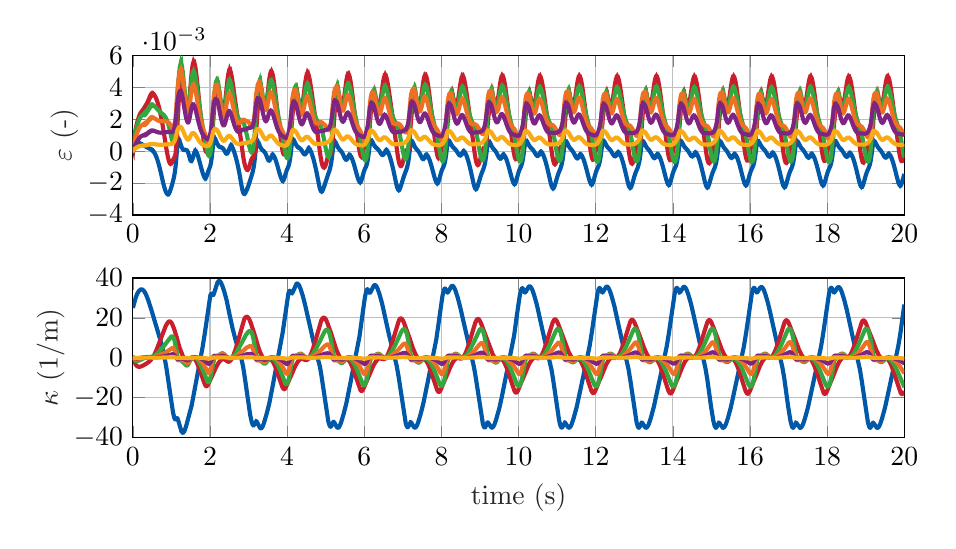
\begin{tikzpicture}

\begin{axis}[%
width=0.808\textwidth,
height=0.167\textwidth,
at={(0\textwidth,0.233\textwidth)},
scale only axis,
xmin=0,
xmax=20,
ymin=-0.004,
ymax=0.006,
ylabel style={font=\color{white!15!black}},
ylabel={$\varepsilon$ (-)},
axis background/.style={fill=white},
xmajorgrids,
ymajorgrids,
ylabel style={yshift=-3.5pt}
]
\addplot [color=mycolor1, line width=1.5pt, forget plot]
  table[row sep=crcr]{%
0	0.000384514542666636\\
0.00833333333333286	0.000438058887421988\\
0.0166666666666657	0.000484030793909795\\
0.0249999999999986	0.00047991929486102\\
0.033333333333335	0.000500820919903333\\
0.0416666666666679	0.000495064395671818\\
0.0500000000000007	0.000503762811501218\\
0.0833333333333321	0.000513190439409783\\
0.091666666666665	0.000521128319476816\\
0.100000000000001	0.000518716877351721\\
0.108333333333334	0.000526601860279641\\
0.116666666666667	0.000522329034588154\\
0.125	0.000528859971193896\\
0.133333333333333	0.000522644857735344\\
0.141666666666666	0.000526959665528182\\
0.149999999999999	0.000518788311683949\\
0.158333333333335	0.000520336473080363\\
0.166666666666668	0.000510418377032806\\
0.175000000000001	0.000508913898837449\\
0.199999999999999	0.000481213753250387\\
0.225000000000001	0.000451352868282129\\
0.283333333333335	0.000368083675148512\\
0.291666666666668	0.000350387996494561\\
0.300000000000001	0.000343085366264262\\
0.308333333333334	0.000324820465301912\\
0.316666666666666	0.000318002249358074\\
0.324999999999999	0.000299835391622594\\
0.333333333333332	0.000293087844546847\\
0.341666666666665	0.000275752701739407\\
0.350000000000001	0.000268652944619419\\
0.358333333333334	0.000252907032471938\\
0.383333333333333	0.000222567653501926\\
0.433333333333334	0.000161773128706244\\
0.441666666666666	0.000160499110414491\\
0.449999999999999	0.000141834285518172\\
0.458333333333332	0.000142576831077434\\
0.466666666666665	0.000120082881046812\\
0.475000000000001	0.000121646256559416\\
0.483333333333334	9.48626155974353e-05\\
0.491666666666667	9.57746346621491e-05\\
0.5	6.4410028176809e-05\\
0.508333333333333	6.30680225306435e-05\\
0.516666666666666	2.70141332592289e-05\\
0.524999999999999	2.1851704342879e-05\\
0.533333333333335	-1.88605002477971e-05\\
0.541666666666668	-2.92153384684468e-05\\
0.550000000000001	-7.44995509904811e-05\\
0.558333333333334	-9.11064071935641e-05\\
0.566666666666666	-0.000140908224206981\\
0.574999999999999	-0.000164461003159033\\
0.583333333333332	-0.000218812026961501\\
0.591666666666665	-0.000249654805550392\\
0.600000000000001	-0.000308677480806097\\
0.608333333333334	-0.000346869071748301\\
0.616666666666667	-0.000410740306197255\\
0.625	-0.000456132384950791\\
0.633333333333333	-0.00052502568798829\\
0.641666666666666	-0.000577323498784921\\
0.649999999999999	-0.000651346154512566\\
0.658333333333335	-0.000710136948640638\\
0.666666666666668	-0.000789269578088891\\
0.675000000000001	-0.000854019629681346\\
0.683333333333334	-0.000938058786189799\\
0.691666666666666	-0.00100808858111989\\
0.699999999999999	-0.00109659100012038\\
0.708333333333332	-0.00117104085602904\\
0.716666666666665	-0.00126326915135166\\
0.725000000000001	-0.00134106746767415\\
0.733333333333334	-0.00143593966057409\\
0.741666666666667	-0.00151578550240572\\
0.75	-0.00161183388197728\\
0.758333333333333	-0.00169220507719103\\
0.766666666666666	-0.00178755314212253\\
0.774999999999999	-0.00186674943948617\\
0.783333333333335	-0.00195911855594844\\
0.791666666666668	-0.0020353446580792\\
0.800000000000001	-0.00212210335501339\\
0.833333333333332	-0.0024037745743648\\
0.850000000000001	-0.00251364504065066\\
0.858333333333334	-0.00256230661168289\\
0.875	-0.00263701003868988\\
0.883333333333333	-0.00265358619581946\\
0.891666666666666	-0.00268250767740597\\
0.899999999999999	-0.00267866915934789\\
0.908333333333335	-0.00269681843051828\\
0.916666666666668	-0.00267214152216866\\
0.925000000000001	-0.00267891699192546\\
0.933333333333334	-0.00263409525881997\\
0.941666666666666	-0.00262899781544945\\
0.949999999999999	-0.00256605994367831\\
0.958333333333332	-0.00254893113863375\\
0.966666666666665	-0.00247131819580559\\
0.975000000000001	-0.00244260208273417\\
0.983333333333334	-0.00235497230046988\\
0.991666666666667	-0.00231582701206534\\
1	-0.00222346756400071\\
1.00833333333333	-0.00217549765773839\\
1.01666666666667	-0.00208321300290137\\
1.025	-0.00202757585857327\\
1.03333333333333	-0.00193789230927877\\
1.04166666666667	-0.00187372551135567\\
1.05	-0.0017845770061804\\
1.05833333333333	-0.00170736665702975\\
1.075	-0.00151171460423427\\
1.08333333333333	-0.00139324225174775\\
1.09166666666667	-0.00126189738345417\\
1.1	-0.00110483730219713\\
1.10833333333333	-0.000930509080788511\\
1.11666666666667	-0.000719118963196763\\
1.125	-0.000499506683084405\\
1.13333333333333	-0.000238129551366484\\
1.14166666666667	-9.50043132164069e-06\\
1.15	0.000229036834415552\\
1.15833333333333	0.000396235279005452\\
1.16666666666667	0.000531735339578177\\
1.175	0.000629427259074333\\
1.18333333333333	0.000661063657087624\\
1.19166666666667	0.000709290673494678\\
1.2	0.000664564939974355\\
1.20833333333333	0.000671584110392587\\
1.21666666666667	0.000588522870494046\\
1.225	0.000560477715232821\\
1.23333333333333	0.00047450203025079\\
1.24166666666667	0.000423348254290801\\
1.25	0.000355798902848647\\
1.25833333333333	0.000296924141924393\\
1.26666666666667	0.00025378025668843\\
1.275	0.000199685945592165\\
1.28333333333333	0.000177751907454393\\
1.29166666666667	0.000135404779467052\\
1.3	0.000128369601654299\\
1.30833333333333	9.95104622845133e-05\\
1.31666666666667	0.000101424662354077\\
1.325	8.43356521471605e-05\\
1.33333333333333	9.06772836373193e-05\\
1.34166666666667	8.1704827760376e-05\\
1.35	8.88458281842475e-05\\
1.35833333333333	8.36333594449457e-05\\
1.36666666666667	8.80671250840237e-05\\
1.39166666666667	6.75323724870225e-05\\
1.4	5.41723636509062e-05\\
1.41666666666667	1.63065360681003e-06\\
1.425	-3.77604482402205e-05\\
1.43333333333333	-8.62298330908118e-05\\
1.44166666666667	-0.00014436058659939\\
1.45833333333333	-0.000285246006807682\\
1.475	-0.000438195097185456\\
1.48333333333333	-0.000505890113743135\\
1.49166666666667	-0.000562664982680872\\
1.5	-0.000602642899707462\\
1.50833333333333	-0.000619312859146959\\
1.51666666666667	-0.000624472592885894\\
1.525	-0.000593551977051021\\
1.53333333333333	-0.000570440534175987\\
1.54166666666667	-0.000498544846347926\\
1.55	-0.000461551475801514\\
1.55833333333333	-0.000364437135125684\\
1.56666666666667	-0.000329343077378752\\
1.575	-0.000225821959112693\\
1.58333333333333	-0.000204878489139304\\
1.59166666666667	-0.000111696014453599\\
1.6	-0.000111245907273627\\
1.60833333333333	-4.03750312543139e-05\\
1.61666666666667	-6.10898710853292e-05\\
1.625	-1.90470612899674e-05\\
1.63333333333333	-5.75416634376325e-05\\
1.64166666666667	-4.61263562350211e-05\\
1.65	-9.72031497141757e-05\\
1.65833333333333	-0.000114567259156928\\
1.66666666666667	-0.000173246958521389\\
1.675	-0.000214942883495439\\
1.7	-0.000402704335332515\\
1.75	-0.000838126323390753\\
1.75833333333333	-0.000922720265901233\\
1.76666666666667	-0.000988119279774935\\
1.775	-0.00107197801834857\\
1.78333333333333	-0.0011346415600606\\
1.79166666666667	-0.00121625131371772\\
1.8	-0.00127404192784297\\
1.80833333333333	-0.0013517575524773\\
1.81666666666667	-0.00140176818406701\\
1.825	-0.00147346295604578\\
1.83333333333333	-0.00151184817628192\\
1.84166666666667	-0.00157465149724345\\
1.85	-0.00159660808773765\\
1.85833333333333	-0.00164683693939338\\
1.86666666666667	-0.00164672385012921\\
1.875	-0.00168011193013129\\
1.88333333333333	-0.00165355855167704\\
1.89166666666667	-0.0016666872102391\\
1.9	-0.00161227055581392\\
1.90833333333333	-0.001604034199854\\
1.91666666666667	-0.00152603506945681\\
1.925	-0.00149953486275578\\
1.93333333333333	-0.00140920153732438\\
1.94166666666667	-0.001371755748103\\
1.95	-0.00128447514119401\\
1.95833333333333	-0.00124421325969948\\
1.96666666666667	-0.00117211465775924\\
1.975	-0.00113183189363752\\
1.98333333333333	-0.00107471065990339\\
1.99166666666667	-0.00102739289447484\\
2	-0.000969685026525724\\
2.00833333333333	-0.00090138503459869\\
2.01666666666667	-0.000820911698973248\\
2.025	-0.000719131691717223\\
2.03333333333333	-0.000598560018232774\\
2.04166666666667	-0.000456851581795092\\
2.05	-0.000285779603707681\\
2.05833333333333	-0.000106475370198922\\
2.06666666666667	0.000105432568979325\\
2.08333333333333	0.00046941839092085\\
2.09166666666667	0.000595285870758744\\
2.1	0.000681093861555127\\
2.10833333333333	0.000748842240749781\\
2.11666666666667	0.000753601052981168\\
2.125	0.00078341146415184\\
2.13333333333333	0.000738201759581614\\
2.14166666666667	0.000739440707356209\\
2.15	0.000672203332239718\\
2.15833333333333	0.000651441142228038\\
2.16666666666667	0.000584071419829968\\
2.175	0.000549274460581728\\
2.18333333333333	0.000494608944734409\\
2.20833333333333	0.000377440853760902\\
2.21666666666667	0.000355850127593982\\
2.225	0.000321783394166886\\
2.23333333333333	0.000312477892379093\\
2.24166666666667	0.0002848918121785\\
2.25	0.00028356367193183\\
2.25833333333333	0.000261949292756469\\
2.26666666666667	0.000264560844858153\\
2.275	0.00024716323989793\\
2.28333333333333	0.000250260534716773\\
2.29166666666667	0.000234586697807515\\
2.3	0.000235219642711115\\
2.30833333333333	0.000218312168289714\\
2.31666666666667	0.000213849097317365\\
2.325	0.000192747602955734\\
2.33333333333333	0.000180995265978368\\
2.34166666666667	0.000153112420459678\\
2.35	0.000132801047701747\\
2.35833333333333	9.67538758800401e-05\\
2.36666666666667	6.85996616134332e-05\\
2.375	2.54740796918895e-05\\
2.38333333333333	-6.55368936008927e-06\\
2.39166666666667	-5.18308961829916e-05\\
2.4	-8.03260037578468e-05\\
2.40833333333333	-0.000118751732923528\\
2.425	-0.000155851816447949\\
2.44166666666667	-0.000148961438306117\\
2.45	-0.000129486100934884\\
2.46666666666667	-6.45386502426959e-05\\
2.475	-6.80503930894361e-06\\
2.48333333333333	2.60815449699692e-05\\
2.49166666666667	9.79791905457716e-05\\
2.5	0.000122169934243743\\
2.50833333333333	0.000196445786386334\\
2.51666666666667	0.00020400476179816\\
2.525	0.000269980169452566\\
2.53333333333333	0.000257082678860598\\
2.54166666666667	0.000307024652567378\\
2.55	0.000274099162528074\\
2.55833333333333	0.000303566265749566\\
2.56666666666667	0.000254392392882608\\
2.575	0.000261663667469492\\
2.58333333333333	0.000201840311465418\\
2.59166666666667	0.000187235533580576\\
2.6	0.00012231486748604\\
2.60833333333333	8.78717882670799e-05\\
2.61666666666667	2.16539479289679e-05\\
2.625	-2.90867871726164e-05\\
2.66666666666667	-0.000365268359274751\\
2.7	-0.000675763079328817\\
2.725	-0.000940583623894042\\
2.74166666666667	-0.00113333119205805\\
2.75833333333333	-0.00134164840032369\\
2.78333333333333	-0.00168322639828489\\
2.80833333333333	-0.00203375580064957\\
2.81666666666667	-0.00215185403784091\\
2.83333333333333	-0.00236077584669303\\
2.84166666666667	-0.00244780544021594\\
2.85	-0.00252624750804031\\
2.85833333333333	-0.00258790876411652\\
2.86666666666667	-0.0026310048153988\\
2.875	-0.00266471682319747\\
2.89166666666667	-0.00267923652960178\\
2.9	-0.0026503118275869\\
2.90833333333333	-0.00264461403751781\\
2.91666666666667	-0.0025920511589419\\
2.925	-0.00257929724080697\\
2.93333333333333	-0.0025130231079622\\
2.94166666666667	-0.00249783359189237\\
2.95	-0.00242459838858267\\
2.95833333333333	-0.00240740198893263\\
2.96666666666667	-0.00233059580223127\\
2.975	-0.00230883716811547\\
2.98333333333333	-0.00222975602558861\\
2.99166666666667	-0.00220038640774689\\
3	-0.00211988472281988\\
3.00833333333333	-0.00208130928945849\\
3.01666666666667	-0.00200089147776339\\
3.025	-0.00195372704982333\\
3.03333333333333	-0.00187570799176484\\
3.04166666666667	-0.00182221054063803\\
3.05	-0.00174888517669203\\
3.05833333333333	-0.001691392063357\\
3.075	-0.00156234720878956\\
3.1	-0.00135904235840556\\
3.11666666666667	-0.00119366645187924\\
3.125	-0.00109343294515796\\
3.13333333333333	-0.000982824618379396\\
3.14166666666667	-0.000855254950177908\\
3.15	-0.000708971630956512\\
3.15833333333333	-0.000548950844489582\\
3.175	-0.000176633822508876\\
3.18333333333333	3.03235778496003e-05\\
3.19166666666667	0.000193414810652826\\
3.2	0.000346787161717543\\
3.20833333333333	0.00044774118993729\\
3.21666666666667	0.000514070915123455\\
3.225	0.000567026594342934\\
3.23333333333333	0.000564966439259962\\
3.24166666666667	0.000586034483877285\\
3.25	0.000541106472059738\\
3.25833333333333	0.000535229280039573\\
3.26666666666667	0.000473318734627526\\
3.275	0.000444206198501718\\
3.28333333333333	0.000385571093598713\\
3.30833333333333	0.000246366756393002\\
3.31666666666667	0.000216360702903984\\
3.325	0.00016993930076481\\
3.33333333333333	0.000151437086650219\\
3.34166666666667	0.000112708378328108\\
3.35	0.0001009284673259\\
3.35833333333333	7.03622356397204e-05\\
3.36666666666667	6.10518071191279e-05\\
3.375	3.63654090804744e-05\\
3.38333333333333	2.59576457821709e-05\\
3.39166666666667	3.46912583282233e-06\\
3.4	-1.13791351346038e-05\\
3.425	-8.86522145755464e-05\\
3.44166666666667	-0.000160578478404005\\
3.45833333333333	-0.00025286652530454\\
3.49166666666667	-0.000462476456721816\\
3.5	-0.00050996476307219\\
3.51666666666667	-0.000570848521771694\\
3.525	-0.000573534622905214\\
3.53333333333333	-0.000584437969074258\\
3.54166666666667	-0.000556692145877946\\
3.55	-0.000552427798066191\\
3.55833333333333	-0.000499752776931928\\
3.56666666666667	-0.000488929786364167\\
3.575	-0.000422292067110419\\
3.58333333333333	-0.000414033657296642\\
3.59166666666667	-0.000346077098512865\\
3.6	-0.000347251946116955\\
3.60833333333333	-0.000289165222643106\\
3.61666666666667	-0.000303180351167498\\
3.625	-0.000262865358948261\\
3.63333333333333	-0.000289981250499949\\
3.64166666666667	-0.000271655299236784\\
3.65	-0.000310096252505332\\
3.65833333333333	-0.000314491837375641\\
3.66666666666667	-0.000361740895961304\\
3.675	-0.000386921811280416\\
3.68333333333333	-0.00044068289818\\
3.69166666666667	-0.000483098651763214\\
3.725	-0.000724355563519907\\
3.74166666666667	-0.000860418001007446\\
3.75	-0.000927031998251948\\
3.75833333333333	-0.00100210970401804\\
3.76666666666667	-0.00106936779125277\\
3.775	-0.00114645142566516\\
3.78333333333333	-0.00121293136417577\\
3.79166666666667	-0.00129034877438272\\
3.8	-0.00135413220202096\\
3.80833333333333	-0.00143010302304347\\
3.81666666666667	-0.00148856046392609\\
3.825	-0.00156088900343576\\
3.83333333333333	-0.00161044453022541\\
3.84166666666667	-0.00167625144593231\\
3.85	-0.00171222559004036\\
3.85833333333333	-0.00176780825820089\\
3.86666666666667	-0.00178457559377776\\
3.875	-0.00182559017765982\\
3.88333333333333	-0.00181713535000227\\
3.89166666666667	-0.00183923573595379\\
3.9	-0.00180179262928704\\
3.90833333333333	-0.00180239457308673\\
3.91666666666667	-0.00173643275504531\\
3.925	-0.00171612535751109\\
3.93333333333333	-0.00162815922174531\\
3.94166666666667	-0.00159151638984412\\
3.95	-0.00149360539075261\\
3.95833333333333	-0.00144822223280983\\
3.96666666666667	-0.00135462653497243\\
3.975	-0.00130837280302032\\
3.98333333333333	-0.00123069907155582\\
3.99166666666667	-0.00118817265204285\\
4	-0.00113028527918146\\
4.01666666666667	-0.00104431564261986\\
4.03333333333333	-0.000947431810729427\\
4.05	-0.000809968826835927\\
4.05833333333333	-0.000716677383984177\\
4.06666666666667	-0.000611071270139263\\
4.075	-0.00048551139480324\\
4.08333333333333	-0.000338649160912752\\
4.09166666666667	-0.000181147704175544\\
4.1	3.70490875312157e-06\\
4.10833333333333	0.000171630091958974\\
4.11666666666667	0.000347246295156367\\
4.125	0.000474022651271611\\
4.13333333333333	0.00057270290920286\\
4.14166666666667	0.000642911699504367\\
4.15	0.000664495184597769\\
4.15833333333333	0.000697732199750334\\
4.16666666666667	0.000669859145386198\\
4.175	0.00067740624486845\\
4.18333333333333	0.00062462211990777\\
4.19166666666667	0.000611779220395903\\
4.2	0.000553832902820517\\
4.20833333333333	0.00052598088439737\\
4.21666666666667	0.000475794885652192\\
4.24166666666667	0.000364247042014654\\
4.25	0.000341196567063662\\
4.25833333333333	0.000305010139392436\\
4.26666666666667	0.000292796343895674\\
4.275	0.000261156438078558\\
4.28333333333333	0.00025578316222763\\
4.29166666666667	0.000228865548997703\\
4.3	0.000226374822929643\\
4.30833333333333	0.000202834586286116\\
4.31666666666667	0.000199775253122425\\
4.325	0.000177297322963454\\
4.33333333333333	0.000170817844555415\\
4.34166666666667	0.000146723613358546\\
4.35	0.000134512910911155\\
4.35833333333333	0.000106320807702787\\
4.36666666666667	8.69902272349066e-05\\
4.425	-0.000148187191999938\\
4.44166666666667	-0.000191617464004423\\
4.45	-0.000200866187643811\\
4.46666666666667	-0.000195925405076736\\
4.475	-0.000171667008576293\\
4.48333333333333	-0.000156489966428808\\
4.49166666666667	-0.000110908165268597\\
4.5	-9.26949405766209e-05\\
4.50833333333333	-3.33652601760548e-05\\
4.51666666666667	-2.02983155972447e-05\\
4.525	4.29086077033958e-05\\
4.53333333333333	4.41831484252475e-05\\
4.54166666666667	0.000101652969842547\\
4.55	8.75541753764253e-05\\
4.55833333333333	0.000131683288593365\\
4.56666666666667	0.000102001298913024\\
4.575	0.000127889681895255\\
4.58333333333333	8.50694128722296e-05\\
4.59166666666667	9.04737933424826e-05\\
4.6	3.82689062909947e-05\\
4.60833333333333	2.32845193650633e-05\\
4.61666666666667	-3.47355257943605e-05\\
4.625	-6.80792576055467e-05\\
4.63333333333333	-0.000129602372108906\\
4.64166666666667	-0.000177989556860325\\
4.675	-0.000437361852331009\\
4.69166666666667	-0.000582827622885418\\
4.70833333333333	-0.000738260281629266\\
4.725	-0.000904265991977127\\
4.74166666666667	-0.00108143035808084\\
4.75833333333333	-0.00127012826962414\\
4.78333333333333	-0.00157420888707094\\
4.83333333333333	-0.00218717707625871\\
4.84166666666667	-0.00227336474217665\\
4.85	-0.00234986375537005\\
4.85833333333333	-0.00241679686498486\\
4.875	-0.0025062754975238\\
4.89166666666667	-0.00253451584616116\\
4.9	-0.0025094159674488\\
4.90833333333333	-0.00250575041779655\\
4.91666666666667	-0.00245128190331556\\
4.925	-0.0024341289836407\\
4.93333333333333	-0.00236035318859606\\
4.94166666666667	-0.00233589442426663\\
4.95	-0.00225205977653431\\
4.95833333333333	-0.00222350880661182\\
4.96666666666667	-0.00213610269368303\\
4.975	-0.0021037103322854\\
4.98333333333333	-0.00201659347826322\\
4.99166666666667	-0.00197930110815747\\
5	-0.00189481108959555\\
5.00833333333333	-0.00185192220304131\\
5.01666666666667	-0.00177194548253468\\
5.025	-0.00172407499267635\\
5.03333333333333	-0.00165050573698267\\
5.04166666666667	-0.00159939626127681\\
5.05	-0.0015336362524927\\
5.06666666666667	-0.00142241691949252\\
5.09166666666667	-0.00125213631591237\\
5.1	-0.00119190660743129\\
5.11666666666667	-0.00104427293199549\\
5.125	-0.000952954364468184\\
5.13333333333333	-0.000853325241450875\\
5.14166666666667	-0.00073684504123861\\
5.15	-0.000604326187687576\\
5.15833333333333	-0.000458459943715184\\
5.175	-0.000118972986506094\\
5.18333333333333	7.15328124982761e-05\\
5.19166666666667	0.00022378102623577\\
5.2	0.0003684211244952\\
5.20833333333333	0.000463243658995083\\
5.21666666666667	0.000526641486629842\\
5.225	0.00057509282074264\\
5.23333333333333	0.000575168799354486\\
5.24166666666667	0.000593956895230008\\
5.25	0.000554884927002064\\
5.25833333333333	0.000549530180020241\\
5.26666666666667	0.000494048772754496\\
5.275	0.000467739035990178\\
5.28333333333333	0.000413651091413669\\
5.3	0.000329560373295124\\
5.30833333333333	0.000282518072495463\\
5.31666666666667	0.000252259913569475\\
5.325	0.000206754435158274\\
5.33333333333333	0.000186564728355876\\
5.34166666666667	0.000146939307285265\\
5.35	0.000132577178629134\\
5.35833333333333	9.96818679723788e-05\\
5.36666666666667	8.71840388647627e-05\\
5.375	5.92596555009095e-05\\
5.38333333333333	4.5308003770117e-05\\
5.39166666666667	1.92123633588892e-05\\
5.4	8.46554495836926e-07\\
5.425	-8.50566153332011e-05\\
5.44166666666667	-0.000158754890904333\\
5.45833333333333	-0.00024728259690221\\
5.48333333333333	-0.000391722287975682\\
5.5	-0.000470566686967544\\
5.51666666666667	-0.000516987704806127\\
5.525	-0.000513333708276775\\
5.53333333333333	-0.000523171207245099\\
5.54166666666667	-0.000494092439701888\\
5.55	-0.000492966459042066\\
5.55833333333333	-0.000444248739036368\\
5.56666666666667	-0.000439568911655641\\
5.575	-0.000381080243787579\\
5.58333333333333	-0.000380242060010971\\
5.59166666666667	-0.000322856635651902\\
5.6	-0.000331153642576965\\
5.60833333333333	-0.000284256307576669\\
5.61666666666667	-0.000304074361277884\\
5.625	-0.000274120316099413\\
5.63333333333333	-0.000305377745700497\\
5.64166666666667	-0.00029562433077146\\
5.65	-0.00033672834984344\\
5.65833333333333	-0.000347438686393531\\
5.66666666666667	-0.000396346828114957\\
5.675	-0.000425557587597325\\
5.68333333333333	-0.000480486548504189\\
5.69166666666667	-0.000524980870512337\\
5.725	-0.000769116853195584\\
5.75	-0.00097503152021261\\
5.79166666666667	-0.0013448182782696\\
5.8	-0.00141285009762271\\
5.80833333333333	-0.00149000057243853\\
5.81666666666667	-0.00155362886304644\\
5.825	-0.00162768675632563\\
5.83333333333333	-0.00168332002044025\\
5.84166666666667	-0.00175129638222415\\
5.85	-0.00179409825442534\\
5.85833333333333	-0.0018520987628996\\
5.86666666666667	-0.00187609628156338\\
5.875	-0.00191953079781726\\
5.88333333333333	-0.00191819310104435\\
5.89166666666667	-0.00194248257108143\\
5.9	-0.00191130688953223\\
5.90833333333333	-0.00191366061049791\\
5.91666666666667	-0.00185228572983931\\
5.925	-0.0018330803047597\\
5.93333333333333	-0.00174719579310789\\
5.94166666666667	-0.00171060564277425\\
5.95	-0.00161108138220456\\
5.95833333333333	-0.00156390493450687\\
5.96666666666667	-0.00146383025714059\\
5.975	-0.00141342962691127\\
5.98333333333333	-0.00132450951549146\\
5.99166666666667	-0.00127663759787211\\
6	-0.00120620101727553\\
6.00833333333333	-0.00116319855424862\\
6.01666666666667	-0.00111166211272717\\
6.04166666666667	-0.000984360522647165\\
6.05	-0.000939626382585601\\
6.06666666666667	-0.000814030767120499\\
6.075	-0.000729147614627834\\
6.08333333333333	-0.000635619163706025\\
6.09166666666667	-0.000522839770859207\\
6.1	-0.000393542634316901\\
6.10833333333333	-0.000251611477672498\\
6.13333333333333	0.000246814349953439\\
6.14166666666667	0.000379899511308679\\
6.15	0.000495231950814912\\
6.15833333333333	0.000573023831645258\\
6.175	0.000649782579941416\\
6.18333333333333	0.000636043199346403\\
6.19166666666667	0.000648511455320744\\
6.2	0.000606000773021975\\
6.20833333333333	0.000598517989420344\\
6.21666666666667	0.000546333254710873\\
6.225	0.000523075135657081\\
6.23333333333333	0.000474697029119397\\
6.25	0.000403420711823088\\
6.25833333333333	0.000365253033240975\\
6.26666666666667	0.000339832643870608\\
6.275	0.000302104134195957\\
6.28333333333333	0.000286796515521104\\
6.29166666666667	0.000252421886642651\\
6.3	0.000243573665173358\\
6.30833333333333	0.000213362317460053\\
6.31666666666667	0.000207150695310077\\
6.325	0.000180243952389247\\
6.33333333333333	0.000173321570073881\\
6.34166666666667	0.000147627787043803\\
6.35	0.000137249160570008\\
6.35833333333333	0.000110358983036463\\
6.36666666666667	9.44940832035002e-05\\
6.375	6.42698018289423e-05\\
6.38333333333333	4.18610451724533e-05\\
6.425	-0.000128136173355387\\
6.45	-0.000210863929673621\\
6.46666666666667	-0.000237612397643971\\
6.48333333333333	-0.000232514694214814\\
6.49166666666667	-0.000206300508690305\\
6.5	-0.00019816409881912\\
6.50833333333333	-0.000154167186249055\\
6.51666666666667	-0.000144857805874921\\
6.525	-9.06415763957114e-05\\
6.53333333333333	-8.69363542648216e-05\\
6.54166666666667	-3.15924654898936e-05\\
6.55	-3.85941192959649e-05\\
6.55833333333333	9.37420057667282e-06\\
6.56666666666667	-1.07216552756029e-05\\
6.575	2.33418040593847e-05\\
6.58333333333333	-9.53839558448522e-06\\
6.59166666666667	6.62087885672236e-06\\
6.6	-3.68744830048229e-05\\
6.60833333333333	-4.00967736560176e-05\\
6.61666666666667	-9.14013551529536e-05\\
6.625	-0.000113275857085426\\
6.63333333333333	-0.000170041472678406\\
6.64166666666667	-0.000208207047148079\\
6.65	-0.000269093068595794\\
6.65833333333333	-0.000320395028399645\\
6.69166666666667	-0.000583973249270286\\
6.71666666666667	-0.000809540459442815\\
6.74166666666667	-0.00105824875907956\\
6.76666666666667	-0.00132886147668287\\
6.79166666666667	-0.00161626311279761\\
6.81666666666667	-0.00190834424390118\\
6.83333333333333	-0.00208995190524419\\
6.84166666666667	-0.00217335202112778\\
6.85833333333333	-0.00231306191067304\\
6.875	-0.00240523604381337\\
6.88333333333333	-0.0024186434572826\\
6.89166666666667	-0.00243985060410523\\
6.9	-0.00241743252161086\\
6.90833333333333	-0.00241635580838917\\
6.91666666666667	-0.0023626143379154\\
6.925	-0.00234497145292778\\
6.93333333333333	-0.0022690270425052\\
6.94166666666667	-0.00224103858863955\\
6.95	-0.00215284546973038\\
6.95833333333333	-0.00211889105048968\\
6.96666666666667	-0.00202645702459137\\
6.975	-0.00198834107472479\\
6.98333333333333	-0.00189706395702416\\
6.99166666666667	-0.00185507819931985\\
7	-0.00176841063244026\\
7.00833333333333	-0.00172271231182464\\
7.01666666666667	-0.00164309043207211\\
7.025	-0.00159458511540578\\
7.03333333333333	-0.00152387549154298\\
7.04166666666667	-0.00147409212131322\\
7.05	-0.00141310489646074\\
7.08333333333333	-0.00120810458979292\\
7.1	-0.00109348120828656\\
7.11666666666667	-0.000949045705660012\\
7.125	-0.000858634465441099\\
7.13333333333333	-0.000759816813339143\\
7.14166666666667	-0.000644353686752197\\
7.15	-0.000512718167527737\\
7.15833333333333	-0.00036906485113164\\
7.18333333333333	0.000142522707353265\\
7.19166666666667	0.00028291396704816\\
7.2	0.000411901125158209\\
7.20833333333333	0.000495683488043852\\
7.21666666666667	0.000546820127706127\\
7.225	0.000588187876378043\\
7.23333333333333	0.00058200767505312\\
7.24166666666667	0.000596016190392845\\
7.25	0.000555898835703061\\
7.25833333333333	0.000547491281110979\\
7.26666666666667	0.000494299344556026\\
7.275	0.000466790700539121\\
7.28333333333333	0.000416125304582238\\
7.325	0.000217303843090377\\
7.33333333333333	0.000197788264390653\\
7.34166666666667	0.000159057241411631\\
7.35	0.000144436193142639\\
7.35833333333333	0.000111622484883611\\
7.36666666666667	9.8166721890891e-05\\
7.375	6.95275082236435e-05\\
7.38333333333333	5.41170248311573e-05\\
7.425	-8.37042144254951e-05\\
7.44166666666667	-0.000158566323989362\\
7.49166666666667	-0.000411428443648276\\
7.5	-0.000446419585919955\\
7.51666666666667	-0.000482000884368006\\
7.525	-0.000472894373874766\\
7.53333333333333	-0.000480823456150858\\
7.54166666666667	-0.000449033354499306\\
7.55	-0.0004486038734548\\
7.55833333333333	-0.000400466603995397\\
7.56666666666667	-0.000398625897936711\\
7.575	-0.00034367046042405\\
7.58333333333333	-0.000346896440792221\\
7.59166666666667	-0.000295107201800704\\
7.6	-0.000307693691251387\\
7.60833333333333	-0.000267351553752349\\
7.61666666666667	-0.00029102292680605\\
7.625	-0.000267700746249488\\
7.63333333333333	-0.000302020879857423\\
7.64166666666667	-0.000298222804833159\\
7.65	-0.000341577042920704\\
7.65833333333333	-0.000357123529504122\\
7.66666666666667	-0.000407664549925357\\
7.675	-0.0004404462226546\\
7.68333333333333	-0.000496651416820981\\
7.69166666666667	-0.000543557217085322\\
7.725	-0.000792505687801537\\
7.75	-0.00100208595867457\\
7.80833333333333	-0.00152815166927667\\
7.81666666666667	-0.00159521955222175\\
7.825	-0.00167076411437606\\
7.83333333333333	-0.00173028539469655\\
7.84166666666667	-0.00179984657151522\\
7.85	-0.00184681848233126\\
7.85833333333333	-0.00190633109305693\\
7.86666666666667	-0.00193450731458356\\
7.875	-0.0019792016342528\\
7.88333333333333	-0.00198174095584491\\
7.89166666666667	-0.00200694636680154\\
7.9	-0.00197904367627544\\
7.90833333333333	-0.00198202395621294\\
7.91666666666667	-0.00192315074260563\\
7.925	-0.00190445052006183\\
7.93333333333333	-0.00182013807839354\\
7.94166666666667	-0.00178394896059331\\
7.95	-0.00168468021464108\\
7.95833333333333	-0.00163745934819559\\
7.96666666666667	-0.00153562393035855\\
7.975	-0.00148414973931565\\
7.98333333333333	-0.00139082686484926\\
7.99166666666667	-0.00134057963708401\\
8	-0.00126341791937534\\
8.00833333333333	-0.00121753081746689\\
8.01666666666667	-0.0011591994948823\\
8.05	-0.000992825056414404\\
8.06666666666667	-0.000892556932747368\\
8.08333333333334	-0.000752003182981298\\
8.09166666666667	-0.000659800116938669\\
8.1	-0.000557450794648418\\
8.10833333333333	-0.000438089044202172\\
8.11666666666667	-0.000300463483451807\\
8.125	-0.000154636412261766\\
8.13333333333333	1.43120335280855e-05\\
8.15	0.000325096134353942\\
8.15833333333333	0.000438658290807581\\
8.16666666666667	0.000527994765356254\\
8.175	0.000589631461711093\\
8.19166666666667	0.000638616362987676\\
8.2	0.000615928576898739\\
8.20833333333334	0.00062130572891661\\
8.21666666666667	0.000576529789043434\\
8.225	0.000563584089253055\\
8.23333333333333	0.000513613523011713\\
8.24166666666667	0.000486437862353029\\
8.25	0.000442411243476215\\
8.275	0.000334282893739157\\
8.28333333333333	0.000312163884899519\\
8.29166666666667	0.000274492639167789\\
8.3	0.000260647199855413\\
8.30833333333333	0.000226635727116786\\
8.31666666666667	0.000217362590340997\\
8.325	0.000187272737196764\\
8.33333333333334	0.000178973641475011\\
8.34166666666667	0.000151472455026891\\
8.35	0.000141146069328357\\
8.35833333333333	0.000114044100495647\\
8.36666666666667	9.9313166526116e-05\\
8.375	7.0274219616806e-05\\
8.38333333333333	4.95719742055201e-05\\
8.45	-0.000211990828944408\\
8.46666666666667	-0.000255040038787513\\
8.48333333333333	-0.00026947639772601\\
8.49166666666667	-0.000254791178008418\\
8.5	-0.000253714803328364\\
8.50833333333333	-0.00021976307522209\\
8.51666666666667	-0.00021412296191059\\
8.525	-0.000166640231544335\\
8.53333333333333	-0.000162914944041859\\
8.54166666666667	-0.000110249485409497\\
8.55	-0.000114136966022471\\
8.55833333333333	-6.49966926324907e-05\\
8.56666666666667	-8.00389126922596e-05\\
8.575	-4.17781573887055e-05\\
8.58333333333334	-6.89355365111055e-05\\
8.59166666666667	-4.66194917798646e-05\\
8.6	-8.4750549998347e-05\\
8.60833333333333	-8.09001480881477e-05\\
8.61666666666667	-0.000127779826744501\\
8.625	-0.00014255751563752\\
8.63333333333333	-0.000195949204861989\\
8.64166666666667	-0.000227657636653333\\
8.65	-0.000286004414128627\\
8.65833333333333	-0.000331853437621987\\
8.69166666666667	-0.000583564228968214\\
8.71666666666667	-0.000801939336387392\\
8.74166666666667	-0.00104209964186452\\
8.76666666666667	-0.00130222387792145\\
8.8	-0.00167096360931751\\
8.825	-0.00194489243970253\\
8.84166666666667	-0.0021102058199105\\
8.85833333333333	-0.00224623036304195\\
8.875	-0.00233835057009202\\
8.88333333333333	-0.0023522525757329\\
8.89166666666667	-0.00237543405451035\\
8.9	-0.00235413162238984\\
8.90833333333333	-0.00235443909809518\\
8.91666666666667	-0.00230103974810447\\
8.925	-0.00228313732794305\\
8.93333333333333	-0.00220602364201383\\
8.94166666666667	-0.0021759623728741\\
8.95	-0.00208534888197676\\
8.95833333333334	-0.00204810697432478\\
8.96666666666667	-0.0019528674585807\\
8.975	-0.00191119061047829\\
8.98333333333333	-0.00181768015343309\\
8.99166666666667	-0.00177274501111668\\
9	-0.0016851509155309\\
9.00833333333333	-0.0016377205803515\\
9.01666666666667	-0.00155886365738311\\
9.025	-0.0015100778855377\\
9.03333333333333	-0.00144179326546734\\
9.04166666666667	-0.00139302208976488\\
9.05	-0.00133561616856426\\
9.08333333333334	-0.00114071215946154\\
9.1	-0.00102811062960129\\
9.11666666666667	-0.00088308028298556\\
9.125	-0.000791825174768945\\
9.13333333333333	-0.000691683523779574\\
9.14166666666667	-0.000575235826612897\\
9.15	-0.000442044805584629\\
9.15833333333333	-0.0002982832153684\\
9.16666666666667	-0.00013043773519783\\
9.175	2.81755088984426e-05\\
9.18333333333333	0.000201408793689239\\
9.19166666666667	0.00033162105703255\\
9.2	0.000446617999749321\\
9.20833333333334	0.00052121072183553\\
9.225	0.00059720236311378\\
9.23333333333333	0.000585335899273787\\
9.24166666666667	0.000595257964036477\\
9.25	0.000553707567394923\\
9.25833333333333	0.000542448400530304\\
9.26666666666667	0.00049066248949714\\
9.275	0.000461740194456439\\
9.28333333333333	0.000413638692908336\\
9.30833333333333	0.000290695066954783\\
9.31666666666667	0.000263946165606654\\
9.325	0.000221100975945632\\
9.33333333333334	0.000202405933869443\\
9.34166666666667	0.000164627841730436\\
9.35	0.000150108710382568\\
9.35833333333333	0.000117695307867649\\
9.36666666666667	0.000103795741772217\\
9.375	7.49511572557537e-05\\
9.38333333333333	5.87020369167135e-05\\
9.425	-8.35401141294767e-05\\
9.44166666666667	-0.000158916096054895\\
9.48333333333333	-0.000368917063731544\\
9.5	-0.000428450980770378\\
9.50833333333333	-0.000437938021587314\\
9.51666666666667	-0.000456042012324076\\
9.525	-0.00044292477925012\\
9.53333333333333	-0.000449307733877191\\
9.54166666666667	-0.000415441560573271\\
9.55	-0.000415262861256593\\
9.55833333333333	-0.000367384653642944\\
9.56666666666667	-0.000367291918980328\\
9.575	-0.000314719152122223\\
9.58333333333334	-0.000320529677619419\\
9.59166666666667	-0.00027260160069531\\
9.6	-0.00028803570002367\\
9.60833333333333	-0.000252376465724069\\
9.61666666666667	-0.000278653660206629\\
9.625	-0.000260120567741495\\
9.63333333333333	-0.000296551985776716\\
9.64166666666667	-0.000297115187031238\\
9.65	-0.000342068256099282\\
9.65833333333333	-0.000361223391589505\\
9.66666666666667	-0.000412975580296404\\
9.675	-0.000448499433296945\\
9.68333333333333	-0.000505695853327381\\
9.69166666666667	-0.000554544233878573\\
9.725	-0.000807627377103159\\
9.75	-0.00102032317347778\\
9.825	-0.00170192436092265\\
9.83333333333334	-0.0017642830239879\\
9.84166666666667	-0.00183501121582808\\
9.85	-0.00188493988286353\\
9.85833333333333	-0.00194546037885956\\
9.86666666666667	-0.00197649609841477\\
9.875	-0.00202190109390443\\
9.88333333333333	-0.00202723269665128\\
9.89166666666667	-0.0020529284431916\\
9.9	-0.00202721089956626\\
9.90833333333333	-0.00203041550735961\\
9.91666666666667	-0.00197326224391503\\
9.925	-0.00195478184841491\\
9.93333333333333	-0.00187176365160369\\
9.94166666666667	-0.00183592018214185\\
9.95	-0.00173735688790444\\
9.95833333333334	-0.00169043509468025\\
9.96666666666667	-0.00158826435739812\\
9.975	-0.00153661260767635\\
9.98333333333333	-0.0014413785395071\\
9.99166666666667	-0.00139009858246197\\
10	-0.00130928673280195\\
10.0083333333333	-0.00126161573767192\\
10.0166666666667	-0.0011986778744344\\
10.0666666666667	-0.000937746466995293\\
10.0833333333333	-0.000815689261489894\\
10.1	-0.000646183566967551\\
10.1083333333333	-0.000539719453417575\\
10.1166666666667	-0.00041910852150906\\
10.125	-0.000285569125818341\\
10.1416666666667	2.21397221658037e-05\\
10.15	0.000191399722474728\\
10.1583333333333	0.000325823734410591\\
10.1666666666667	0.000448408207752493\\
10.175	0.000529970681462544\\
10.1833333333333	0.000578146795405132\\
10.1916666666667	0.000618134993228381\\
10.2	0.000612545029163414\\
10.2083333333333	0.000626533986697098\\
10.2166666666667	0.00059025154972403\\
10.225	0.000584441396743074\\
10.2333333333333	0.00053610511038471\\
10.2416666666667	0.000514163410020529\\
10.25	0.000467372725516668\\
10.2666666666667	0.000396320878532919\\
10.275	0.000357448212149336\\
10.2833333333333	0.000330668181636184\\
10.2916666666667	0.000291441087387767\\
10.3	0.000273899493265617\\
10.3083333333333	0.000237626232770793\\
10.3166666666667	0.000225862298620427\\
10.325	0.000193647467785496\\
10.3333333333333	0.000183999972655613\\
10.3416666666667	0.000155089972874833\\
10.35	0.000144383111507551\\
10.3583333333333	0.000116813405565352\\
10.3666666666667	0.000102476496497417\\
10.375	7.3885699620746e-05\\
10.3833333333333	5.40670768423013e-05\\
10.4333333333333	-0.000142827162477488\\
10.45	-0.000211046380407254\\
10.4666666666667	-0.000263642093479177\\
10.4833333333333	-0.000290377288482802\\
10.4916666666667	-0.000283122818526493\\
10.5	-0.00028703497931204\\
10.5083333333333	-0.000259913683674284\\
10.5166666666667	-0.00025731216594238\\
10.525	-0.000214747735579834\\
10.5333333333333	-0.000211676716162401\\
10.5416666666667	-0.000161330478512411\\
10.55	-0.000163714417528382\\
10.5583333333333	-0.000114273082363781\\
10.5666666666667	-0.000126326340925687\\
10.575	-8.56089811591687e-05\\
10.5833333333333	-0.000109113245606807\\
10.5916666666667	-8.28813761835079e-05\\
10.6	-0.000117406581154\\
10.6083333333333	-0.000108905254016634\\
10.6166666666667	-0.000152669798495708\\
10.625	-0.000162696312386856\\
10.6333333333333	-0.000213603280968755\\
10.6416666666667	-0.000240939924779582\\
10.65	-0.00029734291798178\\
10.6583333333333	-0.000339475821796498\\
10.6916666666667	-0.000582746231994946\\
10.7166666666667	-0.000796064427127874\\
10.7416666666667	-0.00103080523374643\\
10.7666666666667	-0.00128399430301585\\
10.8333333333333	-0.00198803525904623\\
10.8416666666667	-0.00206771427317776\\
10.8583333333333	-0.00220068217418401\\
10.875	-0.00229195244219582\\
10.8833333333333	-0.00230573338173912\\
10.8916666666667	-0.00232993239337276\\
10.9	-0.00230907722518126\\
10.9083333333333	-0.00231018172373965\\
10.9166666666667	-0.00225693853308329\\
10.925	-0.00223889333125982\\
10.9333333333333	-0.0021610980595419\\
10.9416666666667	-0.00212975112897595\\
10.95	-0.00203770022798011\\
10.9583333333333	-0.00199835803923776\\
10.9666666666667	-0.00190145496181771\\
10.975	-0.00185747193724239\\
10.9833333333333	-0.00176271060871613\\
10.9916666666667	-0.00171587407989549\\
11	-0.00162795563922558\\
11.0083333333333	-0.00157946634599071\\
11.0166666666667	-0.00150148510698855\\
11.025	-0.00145265319054033\\
11.0333333333333	-0.00138639308433852\\
11.0833333333333	-0.00109503198261507\\
11.1	-0.000982280781439471\\
11.1166666666667	-0.000834899295337976\\
11.125	-0.000741921138409651\\
11.1333333333333	-0.000639411205177964\\
11.1416666666667	-0.000521007797985362\\
11.15	-0.000385143489253892\\
11.1583333333333	-0.000240234340608936\\
11.1666666666667	-7.1676062795234e-05\\
11.175	8.38296414471529e-05\\
11.1833333333333	0.000249979476492967\\
11.1916666666667	0.00037123586758625\\
11.2	0.000473886486727082\\
11.2083333333333	0.00054083742550759\\
11.225	0.000602973628438974\\
11.2333333333333	0.000586266947081526\\
11.2416666666667	0.000592744500963249\\
11.25	0.000549851972369453\\
11.2583333333333	0.000536094296737843\\
11.2666666666667	0.000485318521761258\\
11.275	0.000455071736514157\\
11.2916666666667	0.000368364459500725\\
11.3	0.000332668654341006\\
11.3083333333333	0.000288683721244354\\
11.3166666666667	0.000263392634128223\\
11.325	0.000221591887743955\\
11.3333333333333	0.000203697353235555\\
11.3416666666667	0.000166820135920176\\
11.35	0.00015253559342554\\
11.3583333333333	0.000120615099891808\\
11.3666666666667	0.00010651385276006\\
11.375	7.76818820114045e-05\\
11.3833333333333	6.09098005384112e-05\\
11.425	-8.41962112474448e-05\\
11.4416666666667	-0.000159793129267172\\
11.4833333333333	-0.000361626645084101\\
11.5	-0.000414741984094746\\
11.5083333333333	-0.000420355796691751\\
11.5166666666667	-0.00043608134677342\\
11.525	-0.000419746502355878\\
11.5333333333333	-0.000424897801131863\\
11.5416666666667	-0.000389244985719017\\
11.55	-0.000389175944636833\\
11.5583333333333	-0.000341256399487122\\
11.5666666666667	-0.000342400622649564\\
11.575	-0.000291398830622569\\
11.5833333333333	-0.000299127395770427\\
11.5916666666667	-0.000253959465752018\\
11.6	-0.000271508809284171\\
11.6083333333333	-0.000239260537810537\\
11.6166666666667	-0.000267482231365079\\
11.625	-0.00025250445214553\\
11.6333333333333	-0.000290523149853783\\
11.6416666666667	-0.000294388614197061\\
11.65	-0.000340554025513029\\
11.6583333333333	-0.000362505708942251\\
11.6666666666667	-0.000415183457668888\\
11.675	-0.000452899466345968\\
11.7083333333333	-0.000684020911108973\\
11.7333333333333	-0.000887651855187244\\
11.7666666666667	-0.00118476230665365\\
11.8083333333333	-0.00157612884842351\\
11.8416666666667	-0.0018615975308478\\
11.85	-0.00191370104493416\\
11.8583333333333	-0.00197496982603695\\
11.8666666666667	-0.00200803700306906\\
11.875	-0.00205389806101763\\
11.8833333333333	-0.00206095596128719\\
11.8916666666667	-0.00208680507479286\\
11.9	-0.00206246545676336\\
11.9083333333333	-0.0020656647770636\\
11.9166666666667	-0.00200961410059008\\
11.925	-0.00199119753177968\\
11.9333333333333	-0.00190906662984958\\
11.9416666666667	-0.00187345654675397\\
11.95	-0.00177554418136339\\
11.9583333333333	-0.00172898967271706\\
11.9666666666667	-0.00162691679089377\\
11.975	-0.0015754275135933\\
11.9833333333333	-0.00147931797479117\\
11.9916666666667	-0.00142765025552549\\
12	-0.00134474926962369\\
12.0083333333333	-0.00129605925740961\\
12.0166666666667	-0.00123010717579675\\
12.075	-0.000911813906220971\\
12.0833333333333	-0.000855997842229783\\
12.1	-0.000701269163041474\\
12.1083333333333	-0.000602699239621529\\
12.1166666666667	-0.000492431761422552\\
12.125	-0.000367296409045537\\
12.1416666666667	-7.41134195827442e-05\\
12.15	9.49115675439316e-05\\
12.1666666666667	0.000380870683539314\\
12.175	0.000477871138695463\\
12.1833333333333	0.000546917806737213\\
12.1916666666667	0.000596528003391938\\
12.2	0.000604731057656238\\
12.2083333333333	0.000625003137688651\\
12.2166666666667	0.000596308981005933\\
12.225	0.00059554379506821\\
12.2333333333333	0.000549691711345446\\
12.2416666666667	0.000531665721226204\\
12.25	0.000483792668472205\\
12.2583333333333	0.000452792927450929\\
12.275	0.000373862520099522\\
12.2833333333333	0.000343888832645689\\
12.2916666666667	0.000303883441819863\\
12.3	0.000283611622798219\\
12.3083333333333	0.000245911456900672\\
12.3166666666667	0.000232213811894866\\
12.325	0.000198536563544849\\
12.3333333333333	0.000187761979088208\\
12.3416666666667	0.000157804851699694\\
12.35	0.000146669050788972\\
12.3583333333333	0.000118662627080823\\
12.3666666666667	0.000104462630321933\\
12.375	7.60630606500001e-05\\
12.3833333333333	5.67670282336508e-05\\
12.425	-0.000103353963023523\\
12.4583333333333	-0.000240285698801301\\
12.4666666666667	-0.000268675757045145\\
12.4833333333333	-0.000303727908924856\\
12.4916666666667	-0.000301625763977853\\
12.5	-0.000309115251834413\\
12.5083333333333	-0.000286894015939509\\
12.5166666666667	-0.000286687333343139\\
12.525	-0.000247825224061415\\
12.5333333333333	-0.000245421416614988\\
12.5416666666667	-0.000196954758163059\\
12.55	-0.000198428608459977\\
12.5583333333333	-0.00014898418297804\\
12.5666666666667	-0.000158998789068221\\
12.575	-0.000116692005423857\\
12.5833333333333	-0.000137606622157449\\
12.5916666666667	-0.000108683803105691\\
12.6	-0.000140587487035049\\
12.6083333333333	-0.000128816594095582\\
12.6166666666667	-0.000170267331697005\\
12.625	-0.000176912656570494\\
12.6333333333333	-0.000225939073320802\\
12.6416666666667	-0.000250140594943105\\
12.65	-0.000305052898053049\\
12.6583333333333	-0.000344509515290525\\
12.6666666666667	-0.000404253738931715\\
12.675	-0.000456065953599705\\
12.7083333333333	-0.000718712024443846\\
12.7333333333333	-0.000942591773885226\\
12.7583333333333	-0.00118631779921685\\
12.7833333333333	-0.00144407433077731\\
12.825	-0.00188043095668533\\
12.8416666666667	-0.0020374428311456\\
12.8583333333333	-0.00216802678862393\\
12.875	-0.00225835108973271\\
12.8833333333333	-0.00227186376774569\\
12.8916666666667	-0.00229660509316076\\
12.9	-0.00227593752601152\\
12.9083333333333	-0.00227748836738328\\
12.9166666666667	-0.00222432695342434\\
12.925	-0.00220613311776319\\
12.9333333333333	-0.00212791746336549\\
12.9416666666667	-0.0020956548766371\\
12.95	-0.00200270334688568\\
12.9583333333333	-0.00196188390565766\\
12.9666666666667	-0.00186395306575804\\
12.975	-0.00181835558428034\\
12.9833333333333	-0.00172289026631134\\
12.9916666666667	-0.0016747435917388\\
13	-0.00158681573325126\\
13.0083333333333	-0.00153764134015333\\
13.0166666666667	-0.00146053655173262\\
13.025	-0.00141176083299399\\
13.0333333333333	-0.00134719300208275\\
13.0833333333333	-0.00106244131340461\\
13.1	-0.000948635266233566\\
13.1166666666667	-0.000798231229637736\\
13.125	-0.000703405541024438\\
13.1333333333333	-0.000598423997935527\\
13.1416666666667	-0.000477896858608773\\
13.15	-0.000339171691020823\\
13.1583333333333	-0.000192878539500896\\
13.1666666666667	-2.35652517268647e-05\\
13.1833333333333	0.000288774565433414\\
13.1916666666667	0.000402299474739465\\
13.2	0.000494565315605655\\
13.2083333333333	0.000555477843306562\\
13.225	0.000606593449795412\\
13.2333333333333	0.00058609999007686\\
13.2416666666667	0.000589785223812811\\
13.25	0.000545879828500517\\
13.2583333333333	0.00053007881868794\\
13.2666666666667	0.000480127507007211\\
13.275	0.000448796799709328\\
13.2916666666667	0.000363608894051737\\
13.3	0.000329471511314239\\
13.3083333333333	0.000286108768289495\\
13.3166666666667	0.000261980639876924\\
13.325	0.000221049294204079\\
13.3333333333333	0.000203816842610394\\
13.3416666666667	0.000167703011122455\\
13.35	0.000153643567308848\\
13.3583333333333	0.00012216714585378\\
13.3666666666667	0.000107951740883294\\
13.375	7.9181905736192e-05\\
13.3833333333333	6.20451533990263e-05\\
13.425	-8.50716363913762e-05\\
13.4416666666667	-0.000160716404124628\\
13.475	-0.000319243274685022\\
13.4833333333333	-0.000355831426137598\\
13.5	-0.000403879558046327\\
13.5083333333333	-0.000406459178403651\\
13.5166666666667	-0.00042033203452263\\
13.525	-0.000401494010525028\\
13.5333333333333	-0.00040567368906963\\
13.5416666666667	-0.000368630031804429\\
13.55	-0.000368607980217206\\
13.5583333333333	-0.00032064179246305\\
13.5666666666667	-0.000322685322288407\\
13.575	-0.000272876888157469\\
13.5833333333333	-0.000282019727940508\\
13.5916666666667	-0.000238963381168134\\
13.6	-0.000258077751663421\\
13.6083333333333	-0.000228450462032015\\
13.6166666666667	-0.000258112734648819\\
13.625	-0.000245879498510959\\
13.6333333333333	-0.000285076201663514\\
13.6416666666667	-0.000291505421081695\\
13.65	-0.000338574605972752\\
13.6583333333333	-0.000362714772254691\\
13.6666666666667	-0.000416088792807301\\
13.675	-0.000455541368445722\\
13.7083333333333	-0.000690077349851492\\
13.7333333333333	-0.000895710776816827\\
13.7666666666667	-0.00119585694373114\\
13.8083333333333	-0.0015919208944517\\
13.8416666666667	-0.00188211439644448\\
13.85	-0.00193587749771496\\
13.8583333333333	-0.00199768937291722\\
13.8666666666667	-0.00203226803765233\\
13.875	-0.00207840717619945\\
13.8833333333333	-0.00208670937401578\\
13.8916666666667	-0.00211257675483267\\
13.9	-0.00208920707872551\\
13.9083333333333	-0.0020923044287855\\
13.9166666666667	-0.00203704559441675\\
13.925	-0.00201861619212451\\
13.9333333333333	-0.00193721007250147\\
13.9416666666667	-0.00190180539980389\\
13.95	-0.00180451141914872\\
13.9583333333333	-0.00175830728366932\\
13.9666666666667	-0.00165651527929711\\
13.975	-0.00160527428431578\\
13.9833333333333	-0.00150878645926511\\
13.9916666666667	-0.00145698958456109\\
14	-0.00137283039740055\\
14.0083333333333	-0.00132351751637216\\
14.0166666666667	-0.00125553431520942\\
14.075	-0.00093666515942914\\
14.0833333333333	-0.000884291822103478\\
14.1	-0.000738892988152884\\
14.1083333333333	-0.000645465314516258\\
14.1166666666667	-0.000541903866199789\\
14.125	-0.000422498869447452\\
14.1416666666667	-0.000140718374531446\\
14.15	2.55341664932018e-05\\
14.1666666666667	0.000326937347235656\\
14.175	0.000435192346788682\\
14.1833333333333	0.000519765110308157\\
14.1916666666667	0.000577198537143886\\
14.2083333333333	0.000621322504688493\\
14.2166666666667	0.000598909025967487\\
14.225	0.00060181600625242\\
14.2333333333333	0.000558436789667383\\
14.2416666666667	0.000543319644819462\\
14.25	0.000495123240973783\\
14.2583333333333	0.000465971848580438\\
14.275	0.000385800668862402\\
14.2833333333333	0.000353530762151166\\
14.2916666666667	0.000313136129037161\\
14.3	0.000290827660787585\\
14.3083333333333	0.000252183978378895\\
14.3166666666667	0.000236997266213734\\
14.325	0.00020228008369827\\
14.3333333333333	0.000190600456551948\\
14.3416666666667	0.000159829885017615\\
14.35	0.000148290778291482\\
14.3583333333333	0.000119904015193129\\
14.3666666666667	0.000105732808364678\\
14.375	7.74068661719696e-05\\
14.3833333333333	5.84452627698795e-05\\
14.425	-9.99447292677758e-05\\
14.4666666666667	-0.000271830029635822\\
14.4833333333333	-0.000312694675667302\\
14.4916666666667	-0.000314274273303994\\
14.5	-0.000324373512953002\\
14.5083333333333	-0.000305760118166631\\
14.5166666666667	-0.000307306163204402\\
14.525	-0.000271246795900737\\
14.5333333333333	-0.000269403412648472\\
14.5416666666667	-0.000222477444197011\\
14.55	-0.000223348739236684\\
14.5583333333333	-0.000174079728715526\\
14.5666666666667	-0.000182627935398472\\
14.575	-0.000139312239308964\\
14.5833333333333	-0.000158313393075815\\
14.5916666666667	-0.000127536602501976\\
14.6	-0.000157468895963575\\
14.6083333333333	-0.000143379922743492\\
14.6166666666667	-0.000183066219033634\\
14.625	-0.000187276450240859\\
14.6333333333333	-0.000234853944771629\\
14.6416666666667	-0.00025677381394118\\
14.65	-0.000310532858698309\\
14.6583333333333	-0.000348027795332939\\
14.6666666666667	-0.000406827121725684\\
14.675	-0.000457050394743419\\
14.7083333333333	-0.000715761717444252\\
14.7333333333333	-0.000936906647261537\\
14.7583333333333	-0.00117767161146887\\
14.7833333333333	-0.00143154700295867\\
14.8166666666667	-0.00177628345590364\\
14.825	-0.00186096351434273\\
14.8416666666667	-0.00201539713040688\\
14.8583333333333	-0.00214411339389642\\
14.875	-0.00223354577877899\\
14.8833333333333	-0.00224677180791488\\
14.8916666666667	-0.00227178446340659\\
14.9	-0.00225119626432146\\
14.9083333333333	-0.00225298017106113\\
14.9166666666667	-0.00219988535003424\\
14.925	-0.00218153301034718\\
14.9333333333333	-0.00210307956530542\\
14.9416666666667	-0.00207012823549491\\
14.95	-0.00197662752092853\\
14.9583333333333	-0.00193472374093062\\
14.9666666666667	-0.00183617271674308\\
14.975	-0.00178940043573661\\
14.9833333333333	-0.00169356838241086\\
14.9916666666667	-0.00164448328299827\\
15	-0.00155671418836079\\
15.0083333333333	-0.00150707674984218\\
15.0166666666667	-0.00143079086431896\\
15.025	-0.00138210609272349\\
15.0333333333333	-0.00131893958544893\\
15.0833333333333	-0.00103878957730075\\
15.1	-0.000923522733327076\\
15.1166666666667	-0.000770026648666544\\
15.125	-0.000673410924335371\\
15.1333333333333	-0.00056606205465215\\
15.1416666666667	-0.00044355135024432\\
15.1583333333333	-0.000154799947829076\\
15.1666666666667	1.49676614569216e-05\\
15.1833333333333	0.000318767062108094\\
15.1916666666667	0.000426028669668455\\
15.2	0.000509953342358926\\
15.2083333333333	0.000566184758067578\\
15.225	0.000608625811580055\\
15.2333333333333	0.000585177914263824\\
15.2416666666667	0.000586606700835546\\
15.25	0.000541941546330804\\
15.2583333333333	0.00052448714068376\\
15.2666666666667	0.000475220826650968\\
15.275	0.000443026006436753\\
15.2916666666667	0.000359079641420124\\
15.3	0.000326223860835029\\
15.3083333333333	0.000283365127685897\\
15.3166666666667	0.000260180262792176\\
15.325	0.00021997114702188\\
15.3333333333333	0.000203282315606401\\
15.3416666666667	0.000167813444690523\\
15.35	0.00015395435942267\\
15.3583333333333	0.000122868963291722\\
15.3666666666667	0.000108588239175589\\
15.375	7.99014056234171e-05\\
15.3833333333333	6.25031876566595e-05\\
15.425	-8.60727545770601e-05\\
15.4416666666667	-0.000161687395486609\\
15.4666666666667	-0.000282909713163804\\
15.4833333333333	-0.000351290065569998\\
15.5	-0.000395296961684721\\
15.5083333333333	-0.000395506869239171\\
15.5166666666667	-0.000407871610349275\\
15.525	-0.000387100132641649\\
15.5333333333333	-0.000390446288601964\\
15.5416666666667	-0.000352349870667013\\
15.55	-0.000352273025900018\\
15.5583333333333	-0.000304308147665466\\
15.5666666666667	-0.000306897051242316\\
15.575	-0.000258019143196009\\
15.5833333333333	-0.000268142827856366\\
15.5916666666667	-0.000226767649724735\\
15.6	-0.000247002076253722\\
15.6083333333333	-0.000219460481982736\\
15.6166666666667	-0.00025016671048661\\
15.625	-0.000240114158724936\\
15.6333333333333	-0.00028017330137331\\
15.6416666666667	-0.000288638823498388\\
15.65	-0.000336379593285585\\
15.6583333333333	-0.000362260648181234\\
15.6666666666667	-0.000416163937487113\\
15.675	-0.000457004025470553\\
15.7083333333333	-0.000694282724413853\\
15.7333333333333	-0.000901550895470393\\
15.7666666666667	-0.00120418551950152\\
15.8083333333333	-0.00160404605244935\\
15.8416666666667	-0.00189795038867047\\
15.8583333333333	-0.00201519717195353\\
15.8666666666667	-0.00205093135232914\\
15.875	-0.00209721528899465\\
15.8833333333333	-0.00210645065692816\\
15.8916666666667	-0.00213223670510487\\
15.9	-0.00210959024400381\\
15.9083333333333	-0.00211250529660845\\
15.9166666666667	-0.0020578582047186\\
15.925	-0.00203932754752145\\
15.9333333333333	-0.00195852635556903\\
15.9416666666667	-0.00192321497366876\\
15.95	-0.00182649530146506\\
15.9583333333333	-0.00178053087857322\\
15.9666666666667	-0.00167910495285639\\
15.975	-0.00162806417372963\\
15.9833333333333	-0.00153148251516555\\
15.9916666666667	-0.0014796310418177\\
16	-0.00139472968965038\\
16.0083333333333	-0.00134499550441092\\
16.0166666666667	-0.0012756509454448\\
16.0583333333333	-0.00104707220037881\\
16.0666666666667	-0.00100712936749758\\
16.0833333333333	-0.00090481184889768\\
16.1	-0.000765559371064484\\
16.1083333333333	-0.00067561494099877\\
16.1166666666667	-0.000576580449255459\\
16.125	-0.000461155072290609\\
16.1333333333333	-0.000329009030323846\\
16.1416666666667	-0.000187692596579581\\
16.15	-2.42645949057874e-05\\
16.1583333333333	0.000126462651468984\\
16.1666666666667	0.000285491758251766\\
16.175	0.000401937114649087\\
16.1833333333333	0.000497968102163071\\
16.1916666666667	0.000561604679063521\\
16.2083333333333	0.000617774292017259\\
16.2166666666667	0.000600421432761067\\
16.225	0.000605956520033146\\
16.2333333333333	0.000564802230268668\\
16.2416666666667	0.000551790935400476\\
16.25	0.000503645336941361\\
16.2583333333333	0.0004759114443047\\
16.275	0.000395068800106202\\
16.3083333333333	0.000257374104659647\\
16.3166666666667	0.000240979037233302\\
16.325	0.000205524484755415\\
16.3333333333333	0.000193065735800246\\
16.3416666666667	0.00016170534347637\\
16.35	0.000149778598256489\\
16.3583333333333	0.000121092789413524\\
16.3666666666667	0.000106863619684816\\
16.375	7.85612545186609e-05\\
16.3833333333333	5.97881188753036e-05\\
16.425	-9.7314994739861e-05\\
16.4666666666667	-0.000273615345822265\\
16.4833333333333	-0.000318644117065503\\
16.4916666666667	-0.000322856154554074\\
16.5	-0.000334962043741172\\
16.5083333333333	-0.000318996973977193\\
16.5166666666667	-0.000321964903783112\\
16.525	-0.000288021829234708\\
16.5333333333333	-0.000286732900878661\\
16.5416666666667	-0.000241029962712247\\
16.55	-0.000241574880590179\\
16.5583333333333	-0.000192534256139965\\
16.5666666666667	-0.000200073843362958\\
16.575	-0.000156108191223581\\
16.5833333333333	-0.000173717864871747\\
16.5916666666667	-0.000141656080366204\\
16.6	-0.00017010489908742\\
16.6083333333333	-0.000154377164353292\\
16.6166666666667	-0.000192694980547969\\
16.625	-0.000195171745676959\\
16.6333333333333	-0.000241590715475581\\
16.6416666666667	-0.00026188499578339\\
16.65	-0.000314694785117808\\
16.6583333333333	-0.000350797547085335\\
16.6666666666667	-0.000408802881544545\\
16.675	-0.0004579087273342\\
16.7083333333333	-0.000713665901500349\\
16.7333333333333	-0.000932744965240317\\
16.7583333333333	-0.00117141209646476\\
16.7833333333333	-0.00142246759323328\\
16.8166666666667	-0.0017630131968005\\
16.825	-0.00184686790859345\\
16.8416666666667	-0.00199938205298622\\
16.8583333333333	-0.00212665518708377\\
16.875	-0.00221532594764184\\
16.8833333333333	-0.00222831382011179\\
16.8916666666667	-0.00225344694108998\\
16.9	-0.00223291411495197\\
16.9083333333333	-0.00223481245584978\\
16.9166666666667	-0.00218180252106137\\
16.925	-0.0021633078871055\\
16.9333333333333	-0.00208474938153103\\
16.9416666666667	-0.0020512894416207\\
16.95	-0.00195747134479518\\
16.9583333333333	-0.00191478051588234\\
16.9666666666667	-0.0018158649778961\\
16.975	-0.00176824598579728\\
16.9833333333333	-0.00167223835660124\\
16.9916666666667	-0.00162248744790006\\
17	-0.00153493324111764\\
17.0083333333333	-0.00148498755923754\\
17.0166666666667	-0.00140940274643242\\
17.025	-0.00136081922108389\\
17.0333333333333	-0.00129876517340932\\
17.0833333333333	-0.00102149234551874\\
17.1	-0.000904644141961342\\
17.1166666666667	-0.000748274791622094\\
17.125	-0.000650024542430572\\
17.1333333333333	-0.000540554809425942\\
17.1416666666667	-0.000416235600546599\\
17.1583333333333	-0.000124201379826161\\
17.1666666666667	4.57617869926707e-05\\
17.1833333333333	0.000342069689580171\\
17.1916666666667	0.000444274326380167\\
17.2	0.000521539043329966\\
17.2083333333333	0.000574108634353365\\
17.2166666666667	0.000588132308340761\\
17.225	0.000609740743282572\\
17.2333333333333	0.000584070873241416\\
17.2416666666667	0.00058362470164397\\
17.25	0.000538450934509882\\
17.2583333333333	0.000519625086287334\\
17.2666666666667	0.000470950956184879\\
17.275	0.00043805617598025\\
17.2916666666667	0.000355121400385627\\
17.3	0.000323260812240989\\
17.3083333333333	0.000280842669074133\\
17.3166666666667	0.000258373745296581\\
17.325	0.000218786351013023\\
17.3333333333333	0.000202498690629938\\
17.3416666666667	0.000167590543291851\\
17.35	0.000153869502241832\\
17.3583333333333	0.000123138907806464\\
17.3666666666667	0.000108796003853939\\
17.375	8.02128700456706e-05\\
17.3833333333333	6.26053345840205e-05\\
17.425	-8.70371763141975e-05\\
17.45	-0.000203073460024683\\
17.475	-0.000314163327278294\\
17.4833333333333	-0.000347830423081064\\
17.5	-0.000388658075806347\\
17.5083333333333	-0.000386961913829253\\
17.5166666666667	-0.000398182520150669\\
17.525	-0.000375845797851326\\
17.5333333333333	-0.000378563018372802\\
17.5416666666667	-0.000339586850859774\\
17.55	-0.000339472076415603\\
17.5583333333333	-0.000291450138618643\\
17.5666666666667	-0.000294497274740735\\
17.575	-0.000246325850959295\\
17.5833333333333	-0.000257202751750896\\
17.5916666666667	-0.000217105680505369\\
17.6	-0.000238178227952801\\
17.6083333333333	-0.000212245073978323\\
17.6166666666667	-0.00024371626765074\\
17.625	-0.000235371446805743\\
17.6333333333333	-0.000276044326053437\\
17.6416666666667	-0.000286131309451321\\
17.65	-0.000334330155606466\\
17.6583333333333	-0.000361624736957111\\
17.6666666666667	-0.000415871273954593\\
17.675	-0.000457865355802056\\
17.7083333333333	-0.000697309790425038\\
17.7333333333333	-0.000905819087787307\\
17.7666666666667	-0.00121045767538419\\
17.8083333333333	-0.00161337485757684\\
17.8416666666667	-0.00191017573990493\\
17.8583333333333	-0.00202869575720044\\
17.8666666666667	-0.00206531251477315\\
17.875	-0.00211167041527105\\
17.8833333333333	-0.00212160968979092\\
17.8916666666667	-0.00214727853249741\\
17.9	-0.00212517524886735\\
17.9083333333333	-0.00212789125270874\\
17.9166666666667	-0.00207371368648168\\
17.925	-0.00205505605184086\\
17.9333333333333	-0.0019747401659771\\
17.9416666666667	-0.00193946941410772\\
17.95	-0.00184323532348785\\
17.9583333333333	-0.00179744548161764\\
17.9666666666667	-0.00169637006657197\\
17.975	-0.0016454957257146\\
17.9833333333333	-0.00154893566950065\\
17.9916666666667	-0.00149707452748871\\
18	-0.00141171366754378\\
18.0083333333333	-0.00136169675523234\\
18.0166666666667	-0.001291409257135\\
18.025	-0.00124481271134158\\
18.0333333333333	-0.00119018718683961\\
18.075	-0.000968945722082282\\
18.0833333333333	-0.000920032743881194\\
18.1	-0.000784775228201084\\
18.1083333333333	-0.000697258084631613\\
18.1166666666667	-0.000601396944436061\\
18.125	-0.000488772292815298\\
18.1333333333333	-0.000360373360937416\\
18.1416666666667	-0.000221469123879103\\
18.15	-6.06632511512828e-05\\
18.1583333333333	9.09629251815147e-05\\
18.1666666666667	0.00025351819250119\\
18.175	0.000375677016556608\\
18.1833333333333	0.000479966732939374\\
18.1916666666667	0.000548403878884329\\
18.2083333333333	0.00061378051179517\\
18.2166666666667	0.000600434833170738\\
18.225	0.000607884054293351\\
18.2333333333333	0.000568640493824546\\
18.2416666666667	0.000557152157561802\\
18.25	0.000509259378176807\\
18.2583333333333	0.000482589578844284\\
18.2666666666667	0.000438089503177252\\
18.2916666666667	0.000325659823651847\\
18.3	0.000300608587277651\\
18.3083333333333	0.000260949024887935\\
18.3166666666667	0.000243636933962676\\
18.325	0.000207693529524988\\
18.3333333333333	0.000194625637977452\\
18.3416666666667	0.000162867502847774\\
18.35	0.000150621703358667\\
18.3583333333333	0.000121737471076244\\
18.3666666666667	0.000107437784187425\\
18.375	7.91644585369511e-05\\
18.3833333333333	6.05102530606416e-05\\
18.425	-9.55934475115328e-05\\
18.4666666666667	-0.000274921804859218\\
18.4833333333333	-0.000322928649442389\\
18.4916666666667	-0.000328999018133658\\
18.5	-0.000342618337544565\\
18.5083333333333	-0.000328546509358318\\
18.5166666666667	-0.000332619997557515\\
18.525	-0.000300202278538109\\
18.5333333333333	-0.000299387663918793\\
18.5416666666667	-0.000254570286628564\\
18.55	-0.000254931967795358\\
18.5583333333333	-0.000206055961204044\\
18.5666666666667	-0.000212889974410047\\
18.575	-0.00016845005612609\\
18.5833333333333	-0.000185046768969244\\
18.5916666666667	-0.000152050882629595\\
18.6	-0.00017939304100878\\
18.6083333333333	-0.000162480193093728\\
18.6166666666667	-0.000199753411088466\\
18.625	-0.000200986081736687\\
18.6333333333333	-0.000246498251684102\\
18.6416666666667	-0.000265638137815216\\
18.65	-0.000317685144576529\\
18.6583333333333	-0.000352813540615671\\
18.6666666666667	-0.000410166572063275\\
18.675	-0.000458505646125928\\
18.7083333333333	-0.000712076091673453\\
18.7333333333333	-0.00092959186198982\\
18.7583333333333	-0.00116677981829838\\
18.7833333333333	-0.00141576544590549\\
18.8166666666667	-0.00175327878030274\\
18.825	-0.00183653629553859\\
18.8416666666667	-0.0019876301598174\\
18.8583333333333	-0.00211380904091385\\
18.875	-0.00220186396059319\\
18.8833333333333	-0.00221465966000522\\
18.8916666666667	-0.00223983408837114\\
18.9	-0.0022193331328495\\
18.9083333333333	-0.00222127478482292\\
18.9166666666667	-0.0021683346644501\\
18.925	-0.00214970827538963\\
18.9333333333333	-0.00207109624437152\\
18.9416666666667	-0.0020372483029405\\
18.95	-0.00194323108926042\\
18.9583333333333	-0.0018999573630154\\
18.9666666666667	-0.00180081487523509\\
18.975	-0.00175257744859181\\
18.9833333333333	-0.00165648854109079\\
18.9916666666667	-0.00160626096896621\\
19	-0.00151892005620979\\
19.0083333333333	-0.00146876905490601\\
19.0166666666667	-0.00139375902899985\\
19.025	-0.00134527454935451\\
19.0333333333333	-0.00128408885662523\\
19.0833333333333	-0.00100871936548685\\
19.1	-0.000890435512676646\\
19.1166666666667	-0.000731632853138819\\
19.125	-0.00063201439982663\\
19.1333333333333	-0.000520794946744729\\
19.1416666666667	-0.000394970727892741\\
19.1583333333333	-0.000100325072644125\\
19.1666666666667	6.95911412833539e-05\\
19.1833333333333	0.000359616174154809\\
19.1916666666667	0.000457877751994573\\
19.2	0.000530023577681504\\
19.2083333333333	0.000579794152354651\\
19.2166666666667	0.000590536223331384\\
19.225	0.000610245461803771\\
19.2333333333333	0.000582971811777355\\
19.2416666666667	0.000581026794002071\\
19.25	0.000535546746554871\\
19.2583333333333	0.000515637631099963\\
19.2666666666667	0.000467466850565756\\
19.275	0.000434040495939314\\
19.2916666666667	0.000351923503487228\\
19.3	0.000320817462061029\\
19.3083333333333	0.000278793029465874\\
19.3166666666667	0.000256818429207328\\
19.325	0.000217744375071049\\
19.3333333333333	0.00020173275916946\\
19.3416666666667	0.000167283096224935\\
19.35	0.000153647905317911\\
19.3583333333333	0.000123212145204832\\
19.3666666666667	0.000108809131379672\\
19.375	8.03235973343419e-05\\
19.3833333333333	6.25483500868995e-05\\
19.425	-8.78674536082258e-05\\
19.45	-0.000203582725614382\\
19.475	-0.000312484284819448\\
19.4833333333333	-0.000345209713984218\\
19.5	-0.000383601236446651\\
19.5083333333333	-0.000380404398516276\\
19.5166666666667	-0.000390798774180467\\
19.525	-0.000367223206733769\\
19.5333333333333	-0.000369506728063129\\
19.5416666666667	-0.000329814114060412\\
19.55	-0.00032970932984\\
19.5583333333333	-0.000281598190195353\\
19.5666666666667	-0.000285022797509527\\
19.575	-0.000237347731506077\\
19.5833333333333	-0.000248812984242619\\
19.5916666666667	-0.00020965715522081\\
19.6	-0.000231367659797144\\
19.6083333333333	-0.000206642305879967\\
19.6166666666667	-0.000238680714254258\\
19.625	-0.000231637781546112\\
19.6333333333333	-0.000272749064464506\\
19.6416666666667	-0.000284091149584498\\
19.65	-0.000332598908158843\\
19.6583333333333	-0.000361006607001002\\
19.6666666666667	-0.000415467286536852\\
19.675	-0.00045838866705239\\
19.7083333333333	-0.000699493482649416\\
19.7333333333333	-0.000908914766768021\\
19.7666666666667	-0.00121511257285434\\
19.8083333333333	-0.0016204134380402\\
19.8416666666667	-0.00191941644780158\\
19.8583333333333	-0.00203888617142312\\
19.8666666666667	-0.00207615798364102\\
19.875	-0.00212255482116674\\
19.8833333333333	-0.00213300919829607\\
19.8916666666667	-0.00215856558233085\\
19.9	-0.00213685529853791\\
19.9083333333333	-0.00213939810631558\\
19.9166666666667	-0.00208556316099262\\
19.925	-0.00206679527187603\\
19.9333333333333	-0.00198684381626535\\
19.9416666666667	-0.0019516010894236\\
19.95	-0.00185574345610817\\
19.9583333333333	-0.0018100945746653\\
19.9666666666667	-0.00170930722918072\\
19.975	-0.00165857859481733\\
19.9833333333333	-0.001562073376288\\
19.9916666666667	-0.00151023403452299\\
20	-0.00142457785488759\\
};
\addplot [color=mycolor2, line width=1.5pt, forget plot]
  table[row sep=crcr]{%
0	0.000290723243939084\\
0.00833333333333286	0.000211841686731162\\
0.0166666666666657	0.000532296526824183\\
0.0249999999999986	0.000578897590823857\\
0.033333333333335	0.000840619401575537\\
0.0416666666666679	0.000900961788545374\\
0.0500000000000007	0.00110632334454763\\
0.0583333333333336	0.00116576817391234\\
0.0666666666666664	0.00132827632896948\\
0.0749999999999993	0.00138474759943108\\
0.0833333333333321	0.00152090478917088\\
0.091666666666665	0.00157277465374506\\
0.100000000000001	0.00169334653254083\\
0.108333333333334	0.00173972771924724\\
0.116666666666667	0.00184989950954417\\
0.125	0.0018906579159399\\
0.133333333333333	0.00199175690644182\\
0.141666666666666	0.00202726962820421\\
0.149999999999999	0.00211830642138011\\
0.158333333333335	0.00214935830017637\\
0.166666666666668	0.00222828985436507\\
0.175000000000001	0.00225606985958393\\
0.183333333333334	0.00232082685080215\\
0.191666666666666	0.00234691672792309\\
0.199999999999999	0.00239614505673913\\
0.216666666666665	0.00245592005506978\\
0.225000000000001	0.00248452939014854\\
0.233333333333334	0.00250324856330053\\
0.241666666666667	0.0025362613030282\\
0.25	0.0025423462714329\\
0.258333333333333	0.00258166188110209\\
0.266666666666666	0.00257807186224568\\
0.274999999999999	0.00262519969176367\\
0.283333333333335	0.00261536707002108\\
0.291666666666668	0.00267127977220838\\
0.300000000000001	0.00265869003310115\\
0.308333333333334	0.00272374072963188\\
0.316666666666666	0.00271150843707346\\
0.324999999999999	0.00278540883827105\\
0.333333333333332	0.00277590767262836\\
0.341666666666665	0.00285774891652579\\
0.350000000000001	0.00285235572301445\\
0.358333333333334	0.0029406526039466\\
0.366666666666667	0.00293965020056675\\
0.375	0.00303240098393331\\
0.383333333333333	0.00303505403561033\\
0.391666666666666	0.00312982195272937\\
0.399999999999999	0.00313460492309403\\
0.408333333333335	0.00322863279396657\\
0.416666666666668	0.00323356010553155\\
0.425000000000001	0.00332392253838876\\
0.433333333333334	0.00332691503771798\\
0.441666666666666	0.00341069862539811\\
0.449999999999999	0.00340991824750247\\
0.458333333333332	0.00348440895510649\\
0.466666666666665	0.00347850300218511\\
0.475000000000001	0.00354135843488379\\
0.483333333333334	0.00352957351307026\\
0.491666666666667	0.00357896502766053\\
0.5	0.00356111693496786\\
0.508333333333333	0.00359583458426371\\
0.516666666666666	0.0035721532773465\\
0.524999999999999	0.00359166660199861\\
0.533333333333335	0.0035625699222237\\
0.541666666666668	0.00356702900077721\\
0.550000000000001	0.0035329016825294\\
0.558333333333334	0.00352305760483773\\
0.566666666666666	0.00348410540121691\\
0.574999999999999	0.00346114353674309\\
0.583333333333332	0.00341735147993205\\
0.591666666666665	0.00338266499085549\\
0.625	0.00318041198323371\\
0.641666666666666	0.00305803952139527\\
0.658333333333335	0.00292189822414102\\
0.675000000000001	0.00277195413942977\\
0.691666666666666	0.00260801494510332\\
0.708333333333332	0.00242984790008549\\
0.725000000000001	0.00223731829548512\\
0.741666666666667	0.00203054387204205\\
0.758333333333333	0.00181005779218069\\
0.774999999999999	0.001576967463361\\
0.800000000000001	0.00120766936055006\\
0.833333333333332	0.000695616462621729\\
0.858333333333334	0.000314261434375851\\
0.875	7.16307677812722e-05\\
0.891666666666666	-0.000154536956038953\\
0.908333333333335	-0.000357127363393772\\
0.925000000000001	-0.000528550732507682\\
0.941666666666666	-0.000661102040066197\\
0.949999999999999	-0.000700500078814059\\
0.958333333333332	-0.000748016180445177\\
0.966666666666665	-0.000760610686693752\\
0.975000000000001	-0.000785152339652484\\
0.983333333333334	-0.000770535059462674\\
0.991666666666667	-0.000773174162272738\\
1	-0.0007342903595422\\
1.00833333333333	-0.000719669031301606\\
1.01666666666667	-0.000663556399949528\\
1.025	-0.000639943450646996\\
1.03333333333333	-0.000577031980707687\\
1.04166666666667	-0.00055428877725916\\
1.05	-0.000494796424618471\\
1.05833333333333	-0.000479329632579351\\
1.06666666666667	-0.000425989967204998\\
1.075	-0.000413731561419439\\
1.08333333333333	-0.000352639376551167\\
1.09166666666667	-0.000323261376355077\\
1.1	-0.000215805001236191\\
1.10833333333333	-0.000133143063397512\\
1.11666666666667	8.75570304970097e-05\\
1.125	0.000264869372383458\\
1.13333333333333	0.000666433557345414\\
1.14166666666667	0.000922664536762596\\
1.15	0.00145407740638603\\
1.15833333333333	0.00169153528949195\\
1.16666666666667	0.00223520757759488\\
1.175	0.00244270222800935\\
1.18333333333333	0.00296475454666378\\
1.19166666666667	0.003171514379261\\
1.2	0.00361905665793572\\
1.20833333333333	0.00383412274977246\\
1.21666666666667	0.00414766065222238\\
1.225	0.00436053904020284\\
1.23333333333333	0.00450790402839019\\
1.24166666666667	0.00469455347263903\\
1.25	0.00468253258052087\\
1.25833333333333	0.00481821480821054\\
1.26666666666667	0.00468061350033366\\
1.275	0.00475241463487919\\
1.28333333333333	0.00453505895687911\\
1.29166666666667	0.00454126306388503\\
1.3	0.00428719423507573\\
1.30833333333333	0.00423764033346785\\
1.31666666666667	0.00397959892394439\\
1.325	0.00389120550238786\\
1.33333333333333	0.00364982315657514\\
1.34166666666667	0.00354288526277458\\
1.35	0.00333081882035557\\
1.35833333333333	0.00322425174739038\\
1.36666666666667	0.00305001943693739\\
1.375	0.00295978366967375\\
1.38333333333333	0.00283010527230942\\
1.39166666666667	0.00276895594579329\\
1.4	0.00268993793800831\\
1.41666666666667	0.0026462987018796\\
1.425	0.00267313777652234\\
1.43333333333333	0.00271643285963918\\
1.44166666666667	0.00280166807323212\\
1.45	0.00291845135579294\\
1.45833333333333	0.00307064217827246\\
1.46666666666667	0.00326015690247417\\
1.475	0.00347731197938472\\
1.48333333333333	0.00371587659875416\\
1.49166666666667	0.0039756222862799\\
1.5	0.00421745207190583\\
1.50833333333333	0.00448446051685636\\
1.51666666666667	0.00469082827554956\\
1.525	0.00493443779446423\\
1.53333333333333	0.00508552828641484\\
1.54166666666667	0.00528435480656952\\
1.55	0.00537103438801623\\
1.55833333333333	0.00551137395723345\\
1.56666666666667	0.00553153241837379\\
1.575	0.00560705007534068\\
1.58333333333333	0.00556518032411191\\
1.59166666666667	0.00557616596319122\\
1.6	0.00548227275113078\\
1.60833333333333	0.00543385578193423\\
1.61666666666667	0.00530042905564443\\
1.625	0.00520055804816266\\
1.63333333333333	0.00504046000304115\\
1.64166666666667	0.00489844220558311\\
1.66666666666667	0.00436600644776775\\
1.675	0.00416946519449013\\
1.68333333333333	0.00398483339230182\\
1.69166666666667	0.00377546284759234\\
1.7	0.00359137438361401\\
1.70833333333333	0.00337709779711304\\
1.71666666666667	0.00319468342314622\\
1.725	0.00298124169757941\\
1.73333333333333	0.00280114098240247\\
1.74166666666667	0.0025921096559216\\
1.75	0.00241493842276341\\
1.75833333333333	0.00221229000074885\\
1.76666666666667	0.00203883170954455\\
1.775	0.00184366400626601\\
1.78333333333333	0.0016750213614678\\
1.79166666666667	0.00148823011230093\\
1.8	0.00132606005790592\\
1.80833333333333	0.00114892965418889\\
1.81666666666667	0.000995804628747265\\
1.825	0.000830568459353032\\
1.83333333333333	0.000690464423513504\\
1.84166666666667	0.000540857205411527\\
1.85833333333333	0.000291382041094579\\
1.875	9.82743475717029e-05\\
1.89166666666667	-2.06520316652359e-05\\
1.9	-3.08770696655358e-05\\
1.90833333333333	-5.04749335554777e-05\\
1.91666666666667	-9.86841394734483e-06\\
1.925	1.14450385559905e-05\\
1.93333333333333	9.6780198262536e-05\\
1.94166666666667	0.000145915541800434\\
1.95	0.000256618729082447\\
1.95833333333333	0.000309890517367961\\
1.96666666666667	0.000416875493886693\\
1.975	0.000448068592707074\\
1.98333333333333	0.000524080031031104\\
1.99166666666667	0.00051867198669342\\
2	0.000555589519198207\\
2.00833333333333	0.000523232134931106\\
2.01666666666667	0.000544662421535946\\
2.025	0.000519004125369094\\
2.03333333333333	0.000579650001892418\\
2.04166666666667	0.000606773396643945\\
2.05	0.000785835636762044\\
2.05833333333333	0.000907328550638908\\
2.06666666666667	0.00127204822437932\\
2.075	0.00146229519277696\\
2.08333333333333	0.0019282727052321\\
2.09166666666667	0.00209199578984709\\
2.1	0.00252377186933472\\
2.10833333333333	0.00266235648024349\\
2.11666666666667	0.00305506471918449\\
2.125	0.00319061121852826\\
2.13333333333333	0.00352286932191603\\
2.14166666666667	0.00365316745942224\\
2.15	0.0038885923095151\\
2.16666666666667	0.00412219397277624\\
2.175	0.00421240615848362\\
2.18333333333333	0.00421337814216116\\
2.19166666666667	0.00427011218771511\\
2.2	0.00417102905072397\\
2.20833333333333	0.00419078364817693\\
2.21666666666667	0.00401907310837757\\
2.225	0.0040053378395335\\
2.23333333333333	0.00379023349844232\\
2.24166666666667	0.00374955596101856\\
2.25	0.00351970200694041\\
2.25833333333333	0.00346131534334759\\
2.26666666666667	0.0032404782853952\\
2.275	0.00317532650313979\\
2.28333333333333	0.00298119417049492\\
2.29166666666667	0.00292087899505233\\
2.3	0.00276582398374359\\
2.30833333333333	0.00272176397771773\\
2.31666666666667	0.0026145920532592\\
2.325	0.00259721311640959\\
2.33333333333333	0.00254440155026359\\
2.34166666666667	0.00256293465886515\\
2.35	0.00256915244478506\\
2.36666666666667	0.00269805942845025\\
2.375	0.00280851456920672\\
2.38333333333333	0.00293110673951347\\
2.4	0.00325238427962304\\
2.40833333333333	0.00345020856432754\\
2.41666666666667	0.00362990259478124\\
2.425	0.00385038199193488\\
2.43333333333333	0.0040213654628154\\
2.44166666666667	0.00424335022175626\\
2.45	0.004384956683257\\
2.45833333333333	0.00458790771850204\\
2.46666666666667	0.00468635594166855\\
2.475	0.00485390927559237\\
2.48333333333333	0.00490144105404511\\
2.49166666666667	0.00502302720934722\\
2.5	0.00501793344573187\\
2.50833333333333	0.00508905569520124\\
2.51666666666667	0.00503511580669169\\
2.525	0.00505645525970877\\
2.53333333333333	0.00496166541728016\\
2.54166666666667	0.00493745157168846\\
2.55	0.00481244385810342\\
2.55833333333333	0.00474868788037952\\
2.56666666666667	0.00460514048052119\\
2.575	0.00450833224885727\\
2.58333333333333	0.00435732260494603\\
2.59166666666667	0.00423399938461699\\
2.60833333333333	0.00394132833273275\\
2.61666666666667	0.00379779296105909\\
2.625	0.00364285142412157\\
2.63333333333333	0.00350666540970934\\
2.64166666666667	0.0033471383691257\\
2.65	0.00321703207658786\\
2.65833333333333	0.0030587076635733\\
2.66666666666667	0.00293278599321667\\
2.675	0.00277889636043227\\
2.68333333333333	0.00265555009505647\\
2.69166666666667	0.00250690641310669\\
2.7	0.00238476463578152\\
2.70833333333333	0.00224064213940167\\
2.71666666666667	0.00211836597867432\\
2.725	0.00197721477766777\\
2.73333333333333	0.0018533637625211\\
2.74166666666667	0.00171325318540028\\
2.75	0.00158626257000805\\
2.75833333333333	0.00144521532516961\\
2.76666666666667	0.00131353973818804\\
2.80833333333333	0.000590610113938794\\
2.85	-0.000149347859185411\\
2.85833333333333	-0.000286349556727572\\
2.86666666666667	-0.000414620475503114\\
2.875	-0.000534508721468541\\
2.89166666666667	-0.000740733581675812\\
2.90833333333333	-0.000902983801072565\\
2.925	-0.00102537940958314\\
2.94166666666667	-0.00111173816111076\\
2.95	-0.00113123618704591\\
2.95833333333333	-0.00116160842757651\\
2.96666666666667	-0.00115948314846293\\
2.975	-0.00117045760804402\\
2.98333333333333	-0.00114440293995699\\
2.99166666666667	-0.00113366725653563\\
3	-0.00108304728305697\\
3.00833333333333	-0.0010510609971135\\
3.01666666666667	-0.000978646845066322\\
3.025	-0.000929936530390307\\
3.03333333333333	-0.000842703535482769\\
3.04166666666667	-0.000786002850841072\\
3.05	-0.000694879465864773\\
3.05833333333333	-0.000641945597191551\\
3.06666666666667	-0.000560050123539213\\
3.075	-0.0005226342803617\\
3.08333333333333	-0.000461260956456044\\
3.09166666666667	-0.000446088529354682\\
3.1	-0.000407487608530488\\
3.10833333333333	-0.000409802926434111\\
3.11666666666667	-0.000380874894563732\\
3.125	-0.000382770707787472\\
3.13333333333333	-0.00033269753286902\\
3.14166666666667	-0.000304435692438432\\
3.15	-0.000182789055489962\\
3.15833333333333	-8.79265223190373e-05\\
3.16666666666667	0.000171174834889598\\
3.175	0.000351368360572479\\
3.18333333333333	0.000771430561382402\\
3.19166666666667	0.00097721514546123\\
3.2	0.00144831950244395\\
3.20833333333333	0.00160517183306297\\
3.21666666666667	0.00204677618602034\\
3.225	0.00217891197500464\\
3.23333333333333	0.00257185577167363\\
3.24166666666667	0.00270997701660747\\
3.25	0.00301154223872757\\
3.25833333333333	0.00316860150926956\\
3.275	0.00351152686028655\\
3.28333333333333	0.00354962207820719\\
3.29166666666667	0.00370972422549798\\
3.3	0.00363489587707733\\
3.30833333333333	0.00376241231189312\\
3.31666666666667	0.00361454156834284\\
3.325	0.00369641812181598\\
3.33333333333333	0.00351571150436669\\
3.34166666666667	0.00355110631529243\\
3.35	0.00336916009615251\\
3.35833333333333	0.00336831968919071\\
3.36666666666667	0.00320460611136042\\
3.375	0.00318377561008987\\
3.38333333333333	0.00304934542489832\\
3.39166666666667	0.00302573769180015\\
3.4	0.00292765199627354\\
3.40833333333333	0.00291655678057623\\
3.41666666666667	0.00286036182332694\\
3.425	0.00287427289800846\\
3.43333333333333	0.0028647940662303\\
3.44166666666667	0.00291353157967222\\
3.45	0.00295450347260129\\
3.46666666666667	0.00313710891321861\\
3.48333333333333	0.00340756146819388\\
3.49166666666667	0.00358115964371564\\
3.5	0.0037421037121419\\
3.50833333333333	0.00393817484654946\\
3.51666666666667	0.00409818080997226\\
3.525	0.00429424753028229\\
3.53333333333333	0.00442925908956582\\
3.54166666666667	0.00460403725465497\\
3.55	0.00469859968679387\\
3.55833333333333	0.00483617109327739\\
3.56666666666667	0.00488300135575415\\
3.575	0.00497346278553934\\
3.58333333333333	0.00497160237249616\\
3.59166666666667	0.00501062569401967\\
3.6	0.00496398721638514\\
3.60833333333333	0.00495197034089045\\
3.61666666666667	0.0048676566881305\\
3.625	0.00480858364172576\\
3.63333333333333	0.00469525223291711\\
3.64166666666667	0.0045955190983058\\
3.65833333333333	0.00432891455963968\\
3.66666666666667	0.00418108004352291\\
3.68333333333333	0.00386741716330619\\
3.69166666666667	0.00369386408566541\\
3.7	0.0035318494307397\\
3.70833333333333	0.00334863029218013\\
3.71666666666667	0.00318339579760618\\
3.725	0.00299570890617318\\
3.73333333333333	0.00282875758980339\\
3.74166666666667	0.00264016419379942\\
3.75	0.00247263548390109\\
3.75833333333333	0.00228539509598491\\
3.76666666666667	0.00211828058610308\\
3.775	0.00193382820065935\\
3.78333333333333	0.00176816977207395\\
3.79166666666667	0.00158760792110613\\
3.8	0.00142474374759161\\
3.80833333333333	0.00124932208456485\\
3.81666666666667	0.00109122296036901\\
3.825	0.000922832865388301\\
3.83333333333333	0.000772554595108943\\
3.84166666666667	0.000614263908726542\\
3.85833333333333	0.000333074681545753\\
3.875	9.28449747839011e-05\\
3.89166666666667	-8.87465365764228e-05\\
3.90833333333333	-0.000193663270817268\\
3.925	-0.000208922309909099\\
3.93333333333333	-0.00016364942664282\\
3.94166666666667	-0.000134062075513697\\
3.95	-4.5217352923288e-05\\
3.95833333333333	1.35572886890145e-05\\
3.96666666666667	0.000130218831856155\\
3.975	0.000199184073185421\\
3.98333333333333	0.000320492293678143\\
3.99166666666667	0.000376735316130805\\
4	0.000476880791701717\\
4.00833333333333	0.000500319732370968\\
4.01666666666667	0.000559559083072259\\
4.025	0.000542738108428864\\
4.03333333333333	0.000559891697179182\\
4.04166666666667	0.000516087977398882\\
4.05	0.000516620343564256\\
4.05833333333333	0.000477042572498476\\
4.06666666666667	0.000509355085522856\\
4.075	0.000514340431688964\\
4.08333333333333	0.000645752866471838\\
4.09166666666667	0.000733560598842331\\
4.1	0.00103167360109779\\
4.10833333333333	0.00119496370216154\\
4.11666666666667	0.00162059310872209\\
4.125	0.00177202313749092\\
4.13333333333333	0.00218171168475934\\
4.14166666666667	0.002295900261025\\
4.15	0.00266086566701773\\
4.15833333333333	0.00276598808220641\\
4.16666666666667	0.00307816707703878\\
4.175	0.00318279408531197\\
4.18333333333333	0.00341144670290205\\
4.19166666666667	0.00351380228972431\\
4.2	0.0036368472775834\\
4.20833333333333	0.00373043577186039\\
4.21666666666667	0.00374498206808127\\
4.225	0.00382131669900687\\
4.23333333333333	0.00374197293467304\\
4.24166666666667	0.00379375898423362\\
4.25	0.00364654182114066\\
4.25833333333333	0.00367247306768093\\
4.26666666666667	0.00348763152677734\\
4.275	0.00348998711208992\\
4.28333333333333	0.00329547522957085\\
4.29166666666667	0.00328081389841728\\
4.3	0.00309940674940634\\
4.30833333333333	0.00307741896278202\\
4.31666666666667	0.00292520363341353\\
4.325	0.00290749616193509\\
4.33333333333333	0.0027949797136344\\
4.34166666666667	0.00279217810322763\\
4.35	0.00272631513301391\\
4.35833333333333	0.00274895262761277\\
4.36666666666667	0.0027339310013339\\
4.375	0.00279028803547376\\
4.38333333333333	0.00282751337611487\\
4.39166666666667	0.00292297995776281\\
4.4	0.00300924634551691\\
4.40833333333333	0.00314464634050182\\
4.41666666666667	0.00326960833204026\\
4.425	0.00343917840638852\\
4.43333333333333	0.0035845044203171\\
4.44166666666667	0.00377541255604186\\
4.45	0.00392006380875287\\
4.45833333333333	0.00411490228974642\\
4.46666666666667	0.00423950601970446\\
4.475	0.00442039653989212\\
4.48333333333333	0.00451069146389571\\
4.49166666666667	0.00466267316997104\\
4.5	0.0047104287087123\\
4.50833333333333	0.00482310189787327\\
4.51666666666667	0.00482567194606176\\
4.525	0.00489362735170928\\
4.53333333333333	0.00485336867033936\\
4.54166666666667	0.00487565838483661\\
4.55	0.00479884768667915\\
4.55833333333333	0.00477787205416291\\
4.56666666666667	0.00467323465061753\\
4.575	0.00461352421685035\\
4.58333333333333	0.00449058263827595\\
4.59166666666667	0.00439791250755306\\
4.6	0.00426532646607569\\
4.60833333333333	0.0041463159587245\\
4.63333333333333	0.00373698321704907\\
4.64166666666667	0.00358711204191664\\
4.65	0.00345327792040706\\
4.65833333333333	0.00329800938253655\\
4.66666666666667	0.00316565482343023\\
4.675	0.0030095146490936\\
4.68333333333333	0.00287807602650147\\
4.69166666666667	0.00272352185280411\\
4.7	0.00259233641551404\\
4.70833333333333	0.00244018816740166\\
4.71666666666667	0.00230852130454196\\
4.725	0.0021583331402546\\
4.73333333333333	0.00202530948887869\\
4.74166666666667	0.00187610953933159\\
4.75	0.00174069560805279\\
4.75833333333333	0.00159122531535161\\
4.76666666666667	0.00145239474090175\\
4.775	0.00130144166267243\\
4.78333333333333	0.00115837370548988\\
4.84166666666667	9.14598743904094e-05\\
4.85833333333333	-0.000198063184978281\\
4.875	-0.000458136461222836\\
4.89166666666667	-0.000674513501753182\\
4.90833333333333	-0.000838593098976048\\
4.925	-0.00094949460311966\\
4.94166666666667	-0.00101050574347283\\
4.95	-0.00101221113262895\\
4.95833333333333	-0.0010246163197607\\
4.96666666666667	-0.00100121292499722\\
4.975	-0.000992403381818718\\
4.98333333333333	-0.000944122582545504\\
4.99166666666667	-0.000914153330548118\\
5	-0.000842497336385861\\
5.00833333333333	-0.000793701533627456\\
5.01666666666667	-0.000703209359731005\\
5.025	-0.000641642361017603\\
5.03333333333333	-0.000540867656436461\\
5.04166666666667	-0.000476581247227159\\
5.05	-0.000377885530053135\\
5.05833333333333	-0.000323646549166057\\
5.06666666666667	-0.00024120593082344\\
5.075	-0.000209095067624787\\
5.08333333333333	-0.000154183608589875\\
5.09166666666667	-0.000150007063673741\\
5.1	-0.000123914058306696\\
5.10833333333333	-0.000140979986227308\\
5.11666666666667	-0.000128209119434786\\
5.125	-0.000146756982069007\\
5.13333333333333	-0.000115185653097427\\
5.14166666666667	-0.000105119887162886\\
5.15	-5.25935423922874e-06\\
5.15833333333333	6.84122667173881e-05\\
5.16666666666667	0.000300096077765488\\
5.175	0.000456550192566851\\
5.18333333333333	0.000847020401199217\\
5.19166666666667	0.00103304291802431\\
5.2	0.00147691414236206\\
5.20833333333333	0.00161608728080154\\
5.21666666666667	0.00202439363195595\\
5.225	0.00213731802546491\\
5.23333333333333	0.00249680148951725\\
5.24166666666667	0.00261485764722735\\
5.25	0.00289181590199306\\
5.25833333333333	0.00302863329156722\\
5.26666666666667	0.00319032198368774\\
5.275	0.00334228781402857\\
5.28333333333333	0.0033806605554787\\
5.29166666666667	0.00352975967579994\\
5.3	0.00346372767813818\\
5.30833333333333	0.00358861352045281\\
5.31666666666667	0.00345402696792263\\
5.325	0.00354154450681321\\
5.33333333333333	0.00337564201236873\\
5.34166666666667	0.00342315538063787\\
5.35	0.00325628777211762\\
5.35833333333333	0.00327156300325271\\
5.36666666666667	0.0031229720174295\\
5.375	0.00312000078857366\\
5.38333333333333	0.00300058393326452\\
5.39166666666667	0.00299494794726129\\
5.4	0.00291132750139411\\
5.40833333333333	0.00291722371841274\\
5.41666666666667	0.00287421041823777\\
5.425	0.00290328447504606\\
5.43333333333333	0.0029045805642447\\
5.44166666666667	0.00296564455691595\\
5.45	0.00301317541392265\\
5.46666666666667	0.00320292849973214\\
5.475	0.00333902078995507\\
5.48333333333333	0.00346517509156286\\
5.49166666666667	0.00363149244595817\\
5.5	0.0037744883799995\\
5.50833333333333	0.00395555856974283\\
5.51666666666667	0.00409297573787981\\
5.525	0.00426934803295964\\
5.53333333333333	0.00438171743301297\\
5.54166666666667	0.00453543924358257\\
5.55	0.00461020210821417\\
5.55833333333333	0.004727857752858\\
5.56666666666667	0.00475924738127986\\
5.575	0.00483263664815681\\
5.58333333333333	0.00482043223504647\\
5.59166666666667	0.00484625445846731\\
5.6	0.00479443801404855\\
5.60833333333333	0.00477351961400174\\
5.61666666666667	0.00468866964361681\\
5.625	0.00462496929620215\\
5.63333333333333	0.00451473747644116\\
5.64166666666667	0.00441433538167502\\
5.65833333333333	0.00415609099546543\\
5.66666666666667	0.00401521115850656\\
5.68333333333333	0.00371458755467557\\
5.69166666666667	0.0035485230862804\\
5.7	0.00339397903870875\\
5.70833333333333	0.00321929698449708\\
5.71666666666667	0.00306119802445082\\
5.725	0.00288229809286022\\
5.73333333333333	0.00272193768012485\\
5.74166666666667	0.00254175644966992\\
5.75	0.00238009329786948\\
5.75833333333333	0.00220044275377873\\
5.76666666666667	0.00203827736590512\\
5.775	0.00186027468897976\\
5.78333333333333	0.00169843095393674\\
5.79166666666667	0.00152293279485605\\
5.8	0.0013624949637574\\
5.80833333333333	0.00119053042146078\\
5.81666666666667	0.00103317418996696\\
5.825	0.000866410836060538\\
5.85	0.000414705932943349\\
5.85833333333333	0.00026854299831669\\
5.875	1.66865216471024e-05\\
5.89166666666667	-0.000182192942986603\\
5.90833333333333	-0.000309927135539567\\
5.925	-0.000352165273660887\\
5.93333333333333	-0.000323674066855517\\
5.94166666666667	-0.000305064229593199\\
5.95	-0.000231368442129565\\
5.95833333333333	-0.00017879757448469\\
5.96666666666667	-7.04235878714599e-05\\
5.975	2.71146821617663e-06\\
5.98333333333333	0.000129153444650143\\
5.99166666666667	0.000205002482161376\\
6	0.000328601141056595\\
6.00833333333333	0.000387315676519506\\
6.01666666666667	0.000485680793641308\\
6.025	0.000509974048323869\\
6.03333333333333	0.000565839438415594\\
6.04166666666667	0.000548912463749218\\
6.05	0.000560836592018887\\
6.05833333333333	0.000514474000382847\\
6.06666666666667	0.000505293996031497\\
6.075	0.000457525840356965\\
6.08333333333333	0.000469754564669245\\
6.09166666666667	0.000457250303632861\\
6.1	0.00054985204057445\\
6.10833333333333	0.000609723710244481\\
6.11666666666667	0.0008498303531006\\
6.125	0.000990700119309906\\
6.13333333333333	0.00137987121791028\\
6.14166666666667	0.00153277064890034\\
6.15	0.00193692915359023\\
6.15833333333333	0.0020458504821832\\
6.16666666666667	0.00240157035403854\\
6.175	0.00249388080464641\\
6.18333333333333	0.00280137360184085\\
6.19166666666667	0.00289399711346405\\
6.2	0.00312846789727672\\
6.20833333333333	0.00322480344238585\\
6.21666666666667	0.00336237769644754\\
6.225	0.00345913115149799\\
6.23333333333333	0.00349296566029622\\
6.24166666666667	0.00358201274696057\\
6.25	0.00352350722037542\\
6.25833333333333	0.00359530243199657\\
6.26666666666667	0.00346886105647215\\
6.275	0.00351884629737498\\
6.28333333333333	0.00335431986244217\\
6.29166666666667	0.00338178215169904\\
6.3	0.00320710468349361\\
6.30833333333333	0.00321654543465044\\
6.31666666666667	0.00305432101700731\\
6.325	0.00305405095344469\\
6.33333333333333	0.00291979048027002\\
6.34166666666667	0.00292129842340572\\
6.35	0.00282480463710399\\
6.35833333333333	0.00283890793522446\\
6.36666666666667	0.00278605938023091\\
6.375	0.00282268830225973\\
6.38333333333333	0.00281662502160529\\
6.39166666666667	0.00288349197943205\\
6.4	0.00292437502386633\\
6.40833333333333	0.00302590467960329\\
6.41666666666667	0.00310938047660869\\
6.425	0.00324518581453148\\
6.43333333333333	0.00336058745660139\\
6.44166666666667	0.00352402350099723\\
6.45	0.00365422136765403\\
6.45833333333333	0.00383259850712747\\
6.46666666666667	0.0039589121193977\\
6.475	0.00413616715728793\\
6.48333333333333	0.00424163894901497\\
6.49166666666667	0.00440195920978326\\
6.5	0.00447462594537029\\
6.50833333333333	0.00460514761033437\\
6.51666666666667	0.0046383991648753\\
6.525	0.00473051681077052\\
6.53333333333333	0.00472296192575783\\
6.54166666666667	0.00477245397714654\\
6.55	0.00472707339234191\\
6.55833333333333	0.00473355416944798\\
6.56666666666667	0.00465652155656926\\
6.575	0.00462251703661209\\
6.58333333333333	0.00452170525874607\\
6.59166666666667	0.00445174362538836\\
6.6	0.00433513985692002\\
6.60833333333333	0.0042350988576132\\
6.63333333333333	0.00385591492173276\\
6.64166666666667	0.00371630967445213\\
6.65	0.00358420898298917\\
6.65833333333333	0.0034348726060287\\
6.66666666666667	0.00330183042331456\\
6.675	0.00314788793374632\\
6.68333333333333	0.00301414354091634\\
6.69166666666667	0.00285893216859989\\
6.7	0.00272437962326322\\
6.70833333333333	0.00256958464604296\\
6.71666666666667	0.00243391437503959\\
6.725	0.00228013025252594\\
6.73333333333333	0.00214291787952803\\
6.74166666666667	0.001989527442678\\
6.75	0.00185004609989647\\
6.75833333333333	0.0016964459606541\\
6.76666666666667	0.00155404465924747\\
6.775	0.00139941816022571\\
6.78333333333333	0.00125357515617353\\
6.80833333333333	0.000790429613370947\\
6.83333333333333	0.000329231603888758\\
6.84166666666667	0.000174834305191496\\
6.85833333333333	-0.000117714473581998\\
6.875	-0.000382300854635531\\
6.89166666666667	-0.000603582696243166\\
6.90833333333333	-0.000769733542139051\\
6.925	-0.000876232560386825\\
6.94166666666667	-0.000924605177385018\\
6.95	-0.000916454847537551\\
6.95833333333333	-0.000918796233811747\\
6.96666666666667	-0.000882765592688628\\
6.975	-0.000862210779384753\\
6.98333333333333	-0.000800227396325681\\
6.99166666666667	-0.000758601597976138\\
7	-0.00067388605645391\\
7.00833333333333	-0.000615181818396593\\
7.01666666666667	-0.00051389611678232\\
7.025	-0.00044565110318473\\
7.03333333333333	-0.000337867613083631\\
7.04166666666667	-0.000271362558859067\\
7.05	-0.000170715254689924\\
7.05833333333333	-0.000119414438650267\\
7.06666666666667	-4.06541306823271e-05\\
7.075	-1.62560334899808e-05\\
7.08333333333333	3.0224543259294e-05\\
7.09166666666667	2.3946586651391e-05\\
7.1	3.97296237224509e-05\\
7.10833333333333	1.26787170380283e-05\\
7.11666666666667	1.71000241664387e-05\\
7.125	-8.2258370568411e-06\\
7.13333333333333	2.00845311582043e-05\\
7.14166666666667	2.79565740015641e-05\\
7.15	0.000131822634266143\\
7.15833333333333	0.000207076268544881\\
7.16666666666667	0.000449000813702582\\
7.175	0.000604395909856947\\
7.18333333333333	0.000997397459570948\\
7.19166666666667	0.00117031173421367\\
7.2	0.00159699729788443\\
7.20833333333333	0.00172177664144613\\
7.21666666666667	0.00210664546346706\\
7.225	0.0022103961869675\\
7.23333333333333	0.0025435742473725\\
7.24166666666667	0.00265452110320297\\
7.25	0.00290447467483901\\
7.25833333333333	0.00303360003496422\\
7.275	0.00331482670939209\\
7.28333333333333	0.00333760602749322\\
7.29166666666667	0.00347672497327167\\
7.3	0.00340355258723335\\
7.30833333333333	0.00351996830649881\\
7.31666666666667	0.00338538296850999\\
7.325	0.00346770639315253\\
7.33333333333333	0.00330677686483583\\
7.34166666666667	0.00335326144601567\\
7.35	0.00319425231971593\\
7.35833333333333	0.00321254259482018\\
7.36666666666667	0.00307339380472271\\
7.375	0.00307669729936677\\
7.38333333333333	0.00296761942393431\\
7.39166666666667	0.00297051759652334\\
7.4	0.00289766223416521\\
7.40833333333333	0.00291339545819369\\
7.41666666666667	0.00288104055337612\\
7.425	0.00292036137532747\\
7.43333333333333	0.00293140555134386\\
7.44166666666667	0.00300212136922795\\
7.45	0.00305718059890836\\
7.45833333333333	0.00316333218085063\\
7.46666666666667	0.00325804504477034\\
7.475	0.00339805188044195\\
7.48333333333333	0.00352184594385463\\
7.49166666666667	0.00368684296779165\\
7.5	0.00382152523135559\\
7.50833333333333	0.00399594855018748\\
7.51666666666667	0.00412098552260076\\
7.525	0.00428675806385925\\
7.53333333333333	0.00438525422501357\\
7.54166666666667	0.00452630207435334\\
7.55	0.00458770696317146\\
7.55833333333333	0.00469228805068411\\
7.56666666666667	0.00471216261094298\\
7.575	0.00477337825080326\\
7.58333333333333	0.00475232118008506\\
7.59166666666667	0.00476778153617019\\
7.6	0.00471009053395477\\
7.60833333333333	0.00468115699588267\\
7.61666666666667	0.00459340921218399\\
7.625	0.00452425516233035\\
7.64166666666667	0.00431032732999981\\
7.65833333333333	0.00405303115455169\\
7.66666666666667	0.00391487159043535\\
7.68333333333333	0.00361914416609466\\
7.69166666666667	0.00345606629759487\\
7.7	0.00330527072664921\\
7.70833333333333	0.00313454347931241\\
7.71666666666667	0.00298025943156688\\
7.725	0.00280577225872491\\
7.73333333333333	0.00264910437225296\\
7.74166666666667	0.00247337721477336\\
7.75	0.00231512341882834\\
7.75833333333333	0.00213965366911495\\
7.76666666666667	0.00198046089962745\\
7.775	0.00180613236081228\\
7.78333333333333	0.00164666892511889\\
7.79166666666667	0.00147415852975996\\
7.8	0.00131534754524409\\
7.80833333333333	0.00114553678524842\\
7.81666666666667	0.0009888884951188\\
7.825	0.000823318358463609\\
7.85833333333333	0.000222571132749039\\
7.875	-3.44994171186386e-05\\
7.89166666666667	-0.000241411346696196\\
7.90833333333333	-0.000380202955927444\\
7.925	-0.000436601806693915\\
7.93333333333333	-0.000417533928921188\\
7.94166666666667	-0.00040600672314639\\
7.95	-0.000342354072689233\\
7.95833333333333	-0.000296079179516795\\
7.96666666666667	-0.00019621567422945\\
7.975	-0.000125916952871563\\
7.98333333333333	-3.16617668616459e-06\\
7.99166666666667	7.6564310070637e-05\\
8	0.000204950824894468\\
8.00833333333333	0.000276764940842611\\
8.01666666666667	0.000390618102070306\\
8.025	0.000436627692071312\\
8.03333333333333	0.000516254814208139\\
8.04166666666667	0.000523459969549833\\
8.05	0.000557747401572328\\
8.05833333333333	0.000526364149667558\\
8.06666666666667	0.000523034752802687\\
8.075	0.000471241339031536\\
8.08333333333334	0.000460259648335182\\
8.09166666666667	0.000419305434217421\\
8.1	0.000447494331929477\\
8.10833333333333	0.000453714045985265\\
8.11666666666667	0.000581942252509293\\
8.125	0.000667536730897922\\
8.13333333333333	0.000953477117590751\\
8.14166666666667	0.00110619728317829\\
8.15	0.00150793366613655\\
8.15833333333333	0.0016444622106313\\
8.16666666666667	0.00202731033182246\\
8.175	0.00212449905448864\\
8.18333333333333	0.00245943303584895\\
8.19166666666667	0.00254709727983027\\
8.2	0.00282755983425176\\
8.20833333333334	0.0029191614743489\\
8.21666666666667	0.00311876082608009\\
8.24166666666667	0.00341641122006564\\
8.25	0.00341663494903699\\
8.25833333333333	0.00350827785878494\\
8.26666666666667	0.00342563175984623\\
8.275	0.00349941925017561\\
8.28333333333333	0.00336181299330107\\
8.29166666666667	0.00341329106275978\\
8.3	0.0032499621708233\\
8.30833333333333	0.00327954645328887\\
8.31666666666667	0.00311673693777692\\
8.325	0.00313028211099109\\
8.33333333333334	0.00298716052851944\\
8.34166666666667	0.00299462754002988\\
8.35	0.00288342545970721\\
8.35833333333333	0.00289552032227292\\
8.36666666666667	0.00282362570791861\\
8.375	0.00285144078570099\\
8.38333333333333	0.00282300202388441\\
8.39166666666667	0.00287553859119072\\
8.4	0.00289213411939571\\
8.40833333333333	0.00297559901848743\\
8.41666666666667	0.00303540922259415\\
8.425	0.00315201281972222\\
8.43333333333333	0.00324810367246897\\
8.44166666666667	0.00339457045453528\\
8.45	0.00351341315078102\\
8.45833333333334	0.00368024543373835\\
8.46666666666667	0.00380477703154369\\
8.475	0.00397773478944785\\
8.48333333333333	0.00409014267649255\\
8.49166666666667	0.00425348512820634\\
8.5	0.00433958195901241\\
8.50833333333333	0.00447929178999473\\
8.51666666666667	0.00453013615832987\\
8.525	0.0046357920165967\\
8.53333333333333	0.00464756638359631\\
8.54166666666667	0.0047130043700534\\
8.55	0.00468659388595327\\
8.55833333333333	0.00470965456398886\\
8.56666666666667	0.00464955963556335\\
8.575	0.00463138411204866\\
8.58333333333334	0.00454436176614692\\
8.59166666666667	0.00448853030713536\\
8.6	0.00438206666476759\\
8.60833333333333	0.00429385680704542\\
8.63333333333333	0.0039339714580251\\
8.65	0.00366986091893295\\
8.65833333333333	0.00352411205519232\\
8.66666666666667	0.00339072954467667\\
8.675	0.0032379995382108\\
8.68333333333333	0.00310282736389311\\
8.69166666666667	0.00294699879348315\\
8.7	0.00281030529556858\\
8.70833333333334	0.00265364557911596\\
8.71666666666667	0.0025154142876076\\
8.725	0.00235889713410842\\
8.73333333333333	0.00221889773883888\\
8.74166666666667	0.00206282724902351\\
8.75	0.00192077130557067\\
8.75833333333333	0.0017643214818186\\
8.76666666666667	0.00161957883130981\\
8.775	0.00146240677070608\\
8.78333333333333	0.00131470522732613\\
8.79166666666667	0.00115642562618845\\
8.8	0.00100584514243707\\
8.825	0.00053538881248727\\
8.85833333333333	-6.57249742381794e-05\\
8.875	-0.000332019004343209\\
8.89166666666667	-0.000555035372091339\\
8.90833333333333	-0.000721214591614228\\
8.925	-0.00082380638604107\\
8.94166666666667	-0.00086301253938359\\
8.95	-0.000847875635052731\\
8.95833333333334	-0.000843179744062894\\
8.96666666666667	-0.000798271527813199\\
8.975	-0.000769545377156788\\
8.98333333333333	-0.000697991904058171\\
8.99166666666667	-0.000648362079175513\\
9	-0.000554695560321505\\
9.00833333333333	-0.000489456547800415\\
9.01666666666667	-0.000381139844211731\\
9.025	-0.000309024903607735\\
9.03333333333333	-0.000197356582805952\\
9.04166666666667	-0.000130600954374671\\
9.05	-3.01736095309479e-05\\
9.05833333333333	1.73531702891694e-05\\
9.06666666666667	9.15682030644405e-05\\
9.075	0.000108830299797802\\
9.08333333333334	0.000147647604674006\\
9.09166666666667	0.000133009905887604\\
9.1	0.000140927192113338\\
9.10833333333333	0.000107228436984741\\
9.11666666666667	0.000107013925326527\\
9.125	7.89388354789367e-05\\
9.13333333333333	0.000108515661835895\\
9.14166666666667	0.000118596595381604\\
9.15	0.000231727759363309\\
9.15833333333333	0.000313147440280659\\
9.16666666666667	0.000570572173828054\\
9.175	0.000728476730031957\\
9.18333333333333	0.00112644560948283\\
9.19166666666667	0.0012891777315609\\
9.2	0.00170163564941106\\
9.20833333333334	0.00181687570790601\\
9.21666666666667	0.00218418951977739\\
9.225	0.00228308439260871\\
9.23333333333333	0.00259598378398707\\
9.24166666666667	0.00270367751006617\\
9.25	0.00293177093379526\\
9.275	0.00331197537199657\\
9.28333333333333	0.00332069019044567\\
9.29166666666667	0.00345191894658825\\
9.3	0.00337144106862652\\
9.30833333333333	0.00348021177181934\\
9.31666666666667	0.00334430708981159\\
9.325	0.0034208848005477\\
9.33333333333334	0.00326297332799896\\
9.34166666666667	0.00330668274002122\\
9.35	0.00315327437605717\\
9.35833333333333	0.00317200058912448\\
9.36666666666667	0.00303987558396557\\
9.375	0.00304643141414118\\
9.38333333333333	0.00294519040475549\\
9.39166666666667	0.00295347211130448\\
9.4	0.00288888873548743\\
9.40833333333333	0.00291140069447238\\
9.41666666666667	0.00288734414313296\\
9.425	0.00293410171367725\\
9.43333333333333	0.00295283716005557\\
9.44166666666667	0.00303079542937112\\
9.45	0.00309190933999659\\
9.45833333333334	0.00320396912775323\\
9.46666666666667	0.0033017059510243\\
9.475	0.00344491379523859\\
9.48333333333333	0.00356751923501974\\
9.49166666666667	0.00373194135080368\\
9.5	0.00386119936358398\\
9.50833333333333	0.00403120739066765\\
9.51666666666667	0.0041478800383743\\
9.525	0.00430630892443418\\
9.53333333333333	0.00439520608167498\\
9.54166666666667	0.00452725072140225\\
9.55	0.00457920756777241\\
9.55833333333333	0.00467430806200753\\
9.56666666666667	0.00468586267700033\\
9.575	0.00473807816921124\\
9.58333333333334	0.00471043160840168\\
9.59166666666667	0.00471806417570519\\
9.6	0.00465587748153951\\
9.60833333333333	0.00462072271132641\\
9.61666666666667	0.00453050581471359\\
9.625	0.00445694321186707\\
9.64166666666667	0.00423973157061042\\
9.65833333333333	0.00398222067516585\\
9.66666666666667	0.00384559168690046\\
9.7	0.00324286639717997\\
9.70833333333334	0.00307465919435046\\
9.71666666666667	0.00292284976186252\\
9.725	0.00275126024822114\\
9.73333333333333	0.00259703163220593\\
9.74166666666667	0.00242428219292989\\
9.75	0.00226831026717633\\
9.75833333333333	0.00209567189363113\\
9.76666666666667	0.00193848816681808\\
9.775	0.00176667572759115\\
9.78333333333333	0.00160883508117493\\
9.79166666666667	0.00143839684395175\\
9.8	0.00128071051184975\\
9.80833333333333	0.00111242725531824\\
9.81666666666667	0.000956298713322923\\
9.825	0.000791633910257161\\
9.85833333333333	0.000189511591074165\\
9.875	-7.05400724925198e-05\\
9.89166666666667	-0.000282404878308995\\
9.90833333333333	-0.000427970081069873\\
9.925	-0.000493409877503126\\
9.94166666666667	-0.000474046691291363\\
9.95	-0.000417570170334614\\
9.95833333333334	-0.000376364467001622\\
9.96666666666667	-0.000283423001707916\\
9.975	-0.00021675522432929\\
9.98333333333333	-9.87496313200609e-05\\
9.99166666666667	-1.91595980147952e-05\\
10	0.000109001854905699\\
10.0083333333333	0.000186114467005893\\
10.0166666666667	0.000306274629615189\\
10.025	0.000363786569760549\\
10.0333333333333	0.000456439079894011\\
10.0416666666667	0.000479321176648284\\
10.05	0.00052962015114133\\
10.0583333333333	0.00051227434180845\\
10.0666666666667	0.000519811142453364\\
10.075	0.000473448654126685\\
10.0833333333333	0.000459680195859846\\
10.0916666666667	0.000410446570036527\\
10.1	0.000414449881255052\\
10.1083333333333	0.00039661444515815\\
10.1166666666667	0.00047230110728691\\
10.125	0.000521378692507568\\
10.1333333333333	0.000732230449891347\\
10.1416666666667	0.000862620806625358\\
10.15	0.00122610569124504\\
10.1583333333333	0.00138081561064141\\
10.1666666666667	0.00177967255200784\\
10.175	0.00189037983397355\\
10.1833333333333	0.00224183675307188\\
10.1916666666667	0.00233024158233519\\
10.2	0.00263358934717317\\
10.2083333333333	0.00272254072180544\\
10.2166666666667	0.00295691054422775\\
10.225	0.00305353982432521\\
10.2333333333333	0.00319479586874039\\
10.2416666666667	0.00329763585650156\\
10.25	0.00333757789807976\\
10.2583333333333	0.00343818443083777\\
10.2666666666667	0.0033875334915372\\
10.275	0.00347442128056485\\
10.2833333333333	0.00335775899962698\\
10.2916666666667	0.00342383166251636\\
10.3	0.00327134348945535\\
10.3083333333333	0.0033140516789949\\
10.3166666666667	0.00315351616471204\\
10.325	0.00317653533900497\\
10.3333333333333	0.00302956824676315\\
10.3416666666667	0.0030415025890953\\
10.35	0.00292225591642392\\
10.3583333333333	0.0029340955732664\\
10.3666666666667	0.00285111108095393\\
10.375	0.00287418273805429\\
10.3833333333333	0.00283236196191794\\
10.3916666666667	0.00287646266330555\\
10.4	0.00287819022617342\\
10.4083333333333	0.00295059648397711\\
10.4166666666667	0.00299539391106052\\
10.425	0.00309981375005464\\
10.4333333333333	0.00318287208160939\\
10.4416666666667	0.00331805158387155\\
10.45	0.00342829779210518\\
10.4583333333333	0.0035868892361961\\
10.4666666666667	0.00370884704256369\\
10.475	0.00387809933249983\\
10.4833333333333	0.00399390835860558\\
10.4916666666667	0.0041584114370643\\
10.5	0.00425262099665247\\
10.5083333333333	0.0043977397095567\\
10.5166666666667	0.00445977158080879\\
10.525	0.00457395988747678\\
10.5333333333333	0.00459834400185599\\
10.5416666666667	0.00467414931661736\\
10.55	0.00466033192414983\\
10.5583333333333	0.00469437759228342\\
10.5666666666667	0.00464569291134254\\
10.575	0.00463812937553953\\
10.5833333333333	0.00456053573144999\\
10.5916666666667	0.00451423551295704\\
10.6	0.00441483147028521\\
10.6083333333333	0.00433461332399432\\
10.6333333333333	0.00398825050142548\\
10.65	0.00372944417032883\\
10.6583333333333	0.00358606963849795\\
10.6666666666667	0.00345260787824486\\
10.675	0.00330062419429566\\
10.6833333333333	0.00316459174447914\\
10.6916666666667	0.00300824794710053\\
10.7	0.00287017664344091\\
10.7083333333333	0.00271213790551883\\
10.7166666666667	0.00257221751843417\\
10.725	0.00241381881140512\\
10.7333333333333	0.00227199750579032\\
10.7416666666667	0.00211363209931648\\
10.75	0.00196968395226449\\
10.7583333333333	0.00181118532845659\\
10.7666666666667	0.00166481020721676\\
10.775	0.00150579569789855\\
10.7833333333333	0.00135678917971305\\
10.7916666666667	0.00119700000466594\\
10.8	0.00104553140628028\\
10.8166666666667	0.000732268684490833\\
10.8333333333333	0.00042064201792158\\
10.8416666666667	0.000264720728004875\\
10.8583333333333	-2.94863820720082e-05\\
10.875	-0.00029631796780194\\
10.8916666666667	-0.000519752381663352\\
10.9083333333333	-0.000685222392920792\\
10.925	-0.000784546774188044\\
10.9416666666667	-0.000816963515884339\\
10.95	-0.000796740152356534\\
10.9583333333333	-0.000787001672225784\\
10.9666666666667	-0.000735693409254168\\
10.975	-0.000701168550701681\\
10.9833333333333	-0.000622786949701748\\
10.9916666666667	-0.000567590094444625\\
11	-0.000467692014364474\\
11.0083333333333	-0.000398148738025128\\
11.0166666666667	-0.00028524661534135\\
11.025	-0.000211050151939673\\
11.0333333333333	-9.74317979363093e-05\\
11.0416666666667	-3.15522541782798e-05\\
11.05	6.74729584027034e-05\\
11.0583333333333	0.000110969422870255\\
11.0666666666667	0.000180451796349956\\
11.075	0.000191349593823276\\
11.0833333333333	0.000223470740174037\\
11.0916666666667	0.000202233816889219\\
11.1	0.000204271255174859\\
11.1083333333333	0.000166029017908187\\
11.1166666666667	0.000163412512346639\\
11.125	0.000135119904140169\\
11.1333333333333	0.000168652488511611\\
11.1416666666667	0.000183412734170219\\
11.15	0.000308415576551369\\
11.1583333333333	0.000398085525109337\\
11.1666666666667	0.000672452432933568\\
11.175	0.000833765855816182\\
11.1833333333333	0.00123581773043924\\
11.1916666666667	0.00139012611408873\\
11.2	0.00179033193902711\\
11.2083333333333	0.001898882946616\\
11.2166666666667	0.00225238500468095\\
11.225	0.00234892629519123\\
11.2333333333333	0.0026456684599161\\
11.2416666666667	0.00275198639570462\\
11.25	0.00296218368833223\\
11.2583333333333	0.00308457037973753\\
11.2666666666667	0.00318717848801953\\
11.275	0.0033186673877168\\
11.2833333333333	0.00331529536819986\\
11.2916666666667	0.00344002208600003\\
11.3	0.00335293853612484\\
11.3083333333333	0.00345498431166291\\
11.3166666666667	0.00331743232734993\\
11.325	0.00338851938341023\\
11.3333333333333	0.00323261711938372\\
11.3416666666667	0.0032730999845576\\
11.35	0.00312391070535156\\
11.3583333333333	0.00314202252969054\\
11.3666666666667	0.00301534949372595\\
11.375	0.00302369454983165\\
11.3833333333333	0.0029286258203669\\
11.3916666666667	0.00294060673612151\\
11.4	0.00288261234185327\\
11.4083333333333	0.0029101586952649\\
11.4166666666667	0.00289278436403251\\
11.425	0.00294530715681773\\
11.4333333333333	0.0029703041377438\\
11.4416666666667	0.00305404144382493\\
11.45	0.00312015968581036\\
11.4583333333333	0.00323706276358138\\
11.4666666666667	0.00333745196238766\\
11.475	0.0034834636922767\\
11.4833333333333	0.00360548733185695\\
11.4916666666667	0.00376984824886151\\
11.5	0.00389530591306553\\
11.5083333333333	0.0040623288920294\\
11.5166666666667	0.00417292701488492\\
11.525	0.00432609230722036\\
11.5333333333333	0.00440786278541339\\
11.5416666666667	0.00453327789999491\\
11.55	0.00457808225183243\\
11.5583333333333	0.00466606279745463\\
11.5666666666667	0.00467119929879445\\
11.575	0.00471653257003268\\
11.5833333333333	0.00468371886793406\\
11.5916666666667	0.00468524911828894\\
11.6	0.00461939433289871\\
11.6083333333333	0.00457926243754869\\
11.6166666666667	0.00448689029967042\\
11.625	0.00440965810739158\\
11.6416666666667	0.00418931311147475\\
11.6583333333333	0.00393100454399686\\
11.6666666666667	0.00379531463876503\\
11.7	0.00319674143742787\\
11.7083333333333	0.00303012190356355\\
11.7166666666667	0.00288007292130743\\
11.725	0.00271039730314016\\
11.7333333333333	0.0025579280985859\\
11.7416666666667	0.00238719675317967\\
11.75	0.00223288590483506\\
11.7583333333333	0.00206219810044672\\
11.7666666666667	0.00190648670087157\\
11.775	0.00173642735347812\\
11.7833333333333	0.00157978381219692\\
11.7916666666667	0.00141080221191814\\
11.8	0.00125395581597232\\
11.8083333333333	0.00108675772982281\\
11.8166666666667	0.000931038774378834\\
11.825	0.000767035283704587\\
11.8583333333333	0.000164201999364622\\
11.875	-9.76862372326082e-05\\
11.8916666666667	-0.000312460199090481\\
11.9083333333333	-0.000462270141834864\\
11.925	-0.000533677976125801\\
11.9416666666667	-0.000521989144434798\\
11.95	-0.000470607590443706\\
11.9583333333333	-0.000433232685946194\\
11.9666666666667	-0.000345545949322457\\
11.975	-0.000282095723122211\\
11.9833333333333	-0.000168264915391347\\
11.9916666666667	-8.99037043744499e-05\\
12	3.67268114267461e-05\\
12.0083333333333	0.000116005640393269\\
12.0166666666667	0.000238775719576978\\
12.025	0.000302709466442508\\
12.0333333333333	0.000402765475907785\\
12.0416666666667	0.000435695674763537\\
12.05	0.000496693521444769\\
12.0583333333333	0.00049002481579663\\
12.0666666666667	0.000507124103474865\\
12.075	0.000467108927022508\\
12.0833333333333	0.000455401083620188\\
12.0916666666667	0.000404426759224918\\
12.1	0.000398224235471645\\
12.1083333333333	0.000368666627547753\\
12.1166666666667	0.000416991312103931\\
12.125	0.000444441195437406\\
12.1333333333333	0.000608732723062388\\
12.1416666666667	0.000718140813997792\\
12.15	0.00104053945467797\\
12.1583333333333	0.00119942375840409\\
12.1666666666667	0.0016007168154637\\
12.175	0.0017257558547179\\
12.1833333333333	0.00209033265506164\\
12.1916666666667	0.00218247207521571\\
12.2	0.00249962429768047\\
12.2083333333333	0.00258787627885226\\
12.2166666666667	0.00284363670649057\\
12.225	0.00293921681734588\\
12.2333333333333	0.00310759327335575\\
12.2416666666667	0.0032116086079661\\
12.25	0.003279162638119\\
12.2583333333333	0.00338459891099419\\
12.2666666666667	0.00335728511883815\\
12.275	0.00345279863645231\\
12.2833333333333	0.0033524554847375\\
12.2916666666667	0.00342793920368933\\
12.3	0.00328451953234321\\
12.3083333333333	0.00333604818786881\\
12.3166666666667	0.00317832095199222\\
12.325	0.00320792658281732\\
12.3333333333333	0.0030591945607803\\
12.3416666666667	0.00307436130944794\\
12.35	0.00295021391130845\\
12.3583333333333	0.00296208712790502\\
12.3666666666667	0.00287198167221447\\
12.375	0.00289197599165902\\
12.3833333333333	0.00284138592454397\\
12.3916666666667	0.00287984189698776\\
12.4	0.00287169058373493\\
12.4083333333333	0.00293660293272779\\
12.4166666666667	0.00297124227393297\\
12.425	0.00306728815844082\\
12.4333333333333	0.00314125157631295\\
12.4416666666667	0.00326849512359928\\
12.45	0.00337282938572869\\
12.4583333333333	0.00352543573438879\\
12.4666666666667	0.00364508664317498\\
12.475	0.00381140886276654\\
12.4833333333333	0.00392922888141811\\
12.4916666666667	0.00409423173267598\\
12.5	0.00419394325340861\\
12.5083333333333	0.00434262042850619\\
12.5166666666667	0.00441237686648321\\
12.525	0.00453241876539678\\
12.5333333333333	0.00456568042342198\\
12.5416666666667	0.00464870375308379\\
12.55	0.00464381102910849\\
12.5583333333333	0.00468557625804422\\
12.5666666666667	0.0046450192658547\\
12.575	0.00464495574878043\\
12.5833333333333	0.00457410417084603\\
12.5916666666667	0.00453455777552847\\
12.6	0.00444021510817194\\
12.6083333333333	0.00436565894879948\\
12.6333333333333	0.00402891603782152\\
12.65	0.00377381680748101\\
12.6583333333333	0.00363207808103638\\
12.6666666666667	0.00349850986290789\\
12.675	0.00334698837583502\\
12.6833333333333	0.00321027866790402\\
12.6916666666667	0.00305348419466966\\
12.7	0.00291436050378024\\
12.7083333333333	0.00275524519958736\\
12.7166666666667	0.00261404910683538\\
12.725	0.00245421106898291\\
12.7333333333333	0.00231102009255579\\
12.7416666666667	0.00215107072455112\\
12.75	0.00200577666773682\\
12.7583333333333	0.00184572136110717\\
12.7666666666667	0.00169813267631724\\
12.775	0.00153771922089163\\
12.7833333333333	0.00138772688088906\\
12.7916666666667	0.00122678688752842\\
12.8	0.00107463110354189\\
12.8083333333333	0.000913468847315357\\
12.8333333333333	0.000447867143662961\\
12.8416666666667	0.000291563646293014\\
12.8583333333333	-2.84051183996326e-06\\
12.875	-0.000269802995777724\\
12.8916666666667	-0.000493185535578533\\
12.9083333333333	-0.000657772819227631\\
12.925	-0.000754414132661196\\
12.9416666666667	-0.000781653503953095\\
12.95	-0.000757615356551611\\
12.9583333333333	-0.00074413060363554\\
12.9666666666667	-0.000688072620594227\\
12.975	-0.000649293911216375\\
12.9833333333333	-0.000565905843366465\\
12.9916666666667	-0.000506713915193302\\
13	-0.000402360762013387\\
13.0083333333333	-0.000329897569983473\\
13.0166666666667	-0.000213931342532447\\
13.025	-0.000138650198550749\\
13.0333333333333	-2.41420659534697e-05\\
13.0416666666667	4.04328323391212e-05\\
13.05	0.000137651743884248\\
13.0583333333333	0.00017739624684765\\
13.0666666666667	0.000242540326102159\\
13.075	0.000248086824615967\\
13.0833333333333	0.000274680968413321\\
13.0916666666667	0.000248381673952025\\
13.1	0.000246137796580115\\
13.1083333333333	0.00020518971301442\\
13.1166666666667	0.000201891270702248\\
13.125	0.000174642341956854\\
13.1333333333333	0.000213019086810817\\
13.1416666666667	0.000233299439237555\\
13.15	0.000370066971854044\\
13.1583333333333	0.000468055030715675\\
13.1666666666667	0.000757553506769426\\
13.175	0.000921773686705762\\
13.1833333333333	0.00132551466128206\\
13.1916666666667	0.00147206930544641\\
13.2	0.00186174404790052\\
13.2083333333333	0.00196596610086885\\
13.2166666666667	0.00230857453078315\\
13.225	0.00240408321950625\\
13.2333333333333	0.00268785226235835\\
13.2416666666667	0.00279362371323444\\
13.25	0.00298939748176963\\
13.2583333333333	0.00311001232197583\\
13.2666666666667	0.0031994220410354\\
13.275	0.00332711509004824\\
13.2833333333333	0.00331404809203661\\
13.2916666666667	0.00343278673335234\\
13.3	0.00334047567026374\\
13.3083333333333	0.00343688104498341\\
13.3166666666667	0.00329801735340496\\
13.325	0.00336440399433258\\
13.3333333333333	0.00321009342094669\\
13.3416666666667	0.00324766463193882\\
13.35	0.00310182985229801\\
13.3583333333333	0.00311913173835165\\
13.3666666666667	0.00299680311418982\\
13.375	0.0030063044035451\\
13.3833333333333	0.00291616518484261\\
13.3916666666667	0.00293089445214889\\
13.4	0.00287817560398196\\
13.4083333333333	0.00290961006544777\\
13.4166666666667	0.00289759746169338\\
13.425	0.00295465705264775\\
13.4333333333333	0.00298468078175418\\
13.4416666666667	0.00307300775429198\\
13.45	0.00314313768226882\\
13.4583333333333	0.00326389946901529\\
13.4666666666667	0.00336642949323362\\
13.475	0.00351468808201716\\
13.4833333333333	0.00363633404885633\\
13.4916666666667	0.00380070427372559\\
13.5	0.00392332508327797\\
13.5083333333333	0.0040880950249651\\
13.5166666666667	0.00419412075917691\\
13.525	0.00434326413484953\\
13.5333333333333	0.00441963184019656\\
13.5416666666667	0.00453994468939101\\
13.55	0.00457928643535155\\
13.5583333333333	0.00466175191316864\\
13.5666666666667	0.00466195132909419\\
13.575	0.00470191836009093\\
13.5833333333333	0.00466509664438419\\
13.5916666666667	0.0046618317078817\\
13.6	0.00459309742285186\\
13.6083333333333	0.00454901471729841\\
13.6166666666667	0.00445490912354884\\
13.625	0.00437471995869387\\
13.6416666666667	0.00415174054714385\\
13.6583333333333	0.00389259267908315\\
13.6666666666667	0.00375753572848581\\
13.675	0.00360822543982309\\
13.6833333333333	0.00346699583480259\\
13.6916666666667	0.00330733561667529\\
13.7	0.00316175543293085\\
13.7083333333333	0.00299624861685999\\
13.7166666666667	0.00284749293354736\\
13.725	0.00267919402088879\\
13.7333333333333	0.00252802707991506\\
13.7416666666667	0.00235876715058225\\
13.75	0.00220569126809167\\
13.7583333333333	0.00203643800864839\\
13.7666666666667	0.00188182369183565\\
13.775	0.00171306199756316\\
13.7833333333333	0.0015573110979048\\
13.7916666666667	0.0013894143740032\\
13.8	0.00123319483309814\\
13.8083333333333	0.00106681283870458\\
13.8166666666667	0.000911403071111039\\
13.825	0.000747910928403428\\
13.8583333333333	0.000144698369744845\\
13.875	-0.000118387552969779\\
13.8916666666667	-0.000335083059553654\\
13.9083333333333	-0.000487766406166656\\
13.925	-0.000563340968565029\\
13.9416666666667	-0.000557313179559316\\
13.95	-0.000509742184398476\\
13.9583333333333	-0.000475340591222562\\
13.9666666666667	-0.000391721960500746\\
13.975	-0.000330962339919694\\
13.9833333333333	-0.000220605523921336\\
13.9916666666667	-0.000143691384149491\\
14	-1.88496178701314e-05\\
14.0083333333333	6.12443735334978e-05\\
14.0166666666667	0.000185007355060662\\
14.025	0.00025274829964772\\
14.0333333333333	0.000357230237874262\\
14.0416666666667	0.000396817366755897\\
14.05	0.00046505178688605\\
14.0583333333333	0.000466167299340015\\
14.0666666666667	0.000490618383675923\\
14.075	0.000456262376644645\\
14.0833333333333	0.000447801847716534\\
14.0916666666667	0.000397411840285855\\
14.1	0.000386702608977885\\
14.1083333333333	0.000351027863665365\\
14.1166666666667	0.000383747262290512\\
14.125	0.000397934181918913\\
14.1333333333333	0.000532817179852429\\
14.1416666666667	0.00062642931274226\\
14.15	0.000916158881192786\\
14.1583333333333	0.00107348387444262\\
14.1666666666667	0.0014698931374042\\
14.175	0.00160646411850252\\
14.1833333333333	0.0019808336640601\\
14.1916666666667	0.00207778822191074\\
14.2	0.00240422050955758\\
14.2083333333333	0.00249282985309307\\
14.2166666666667	0.00276256694738919\\
14.225	0.00285760698471904\\
14.2333333333333	0.00304454097808105\\
14.2416666666667	0.00314906913859758\\
14.25	0.00323630090732507\\
14.2583333333333	0.00334459004518806\\
14.2666666666667	0.00333449618822002\\
14.275	0.00343519093211953\\
14.2833333333333	0.00334737777301441\\
14.2916666666667	0.00342923141738183\\
14.3	0.00329312144581451\\
14.3083333333333	0.00335082421493382\\
14.3166666666667	0.00319577181571518\\
14.325	0.00323010982035754\\
14.3333333333333	0.0030806094916116\\
14.3416666666667	0.0030984495065276\\
14.35	0.00297119794588951\\
14.3583333333333	0.00298319915472334\\
14.3666666666667	0.00288831864614636\\
14.375	0.00290620643314554\\
14.3833333333333	0.0028496167152916\\
14.3916666666667	0.00288411878694461\\
14.4	0.0028691256382416\\
14.4083333333333	0.00292874003870836\\
14.4166666666667	0.0029562452059686\\
14.425	0.0030463085304433\\
14.4333333333333	0.00311373878510324\\
14.4416666666667	0.00323521175694452\\
14.45	0.00333480507952189\\
14.4583333333333	0.00348291032643999\\
14.4666666666667	0.00360064397763438\\
14.475	0.00376460109089649\\
14.4833333333333	0.00388362564174116\\
14.4916666666667	0.00404873329800637\\
14.5	0.00415227897779857\\
14.5083333333333	0.00430331079972746\\
14.5166666666667	0.00437866727252256\\
14.525	0.00450277292346613\\
14.5333333333333	0.00454250906875586\\
14.5416666666667	0.00463064991178186\\
14.55	0.00463231250025586\\
14.5583333333333	0.00467961286928542\\
14.5666666666667	0.00464505523621739\\
14.575	0.0046504088698569\\
14.5833333333333	0.00458455423295945\\
14.5916666666667	0.00454991096851032\\
14.6	0.00445933273375942\\
14.6083333333333	0.00438890326201857\\
14.6166666666667	0.00428037861972186\\
14.625	0.00417992016838298\\
14.6416666666667	0.00393540997235675\\
14.65	0.00380689376679655\\
14.6833333333333	0.00324429550822458\\
14.6916666666667	0.00308717588323404\\
14.7	0.00294724674907343\\
14.7083333333333	0.00278733960302446\\
14.7166666666667	0.00264517319306989\\
14.725	0.00248427067226586\\
14.7333333333333	0.00234004070799898\\
14.7416666666667	0.00217891632999923\\
14.75	0.00203260105461567\\
14.7583333333333	0.00187138845851464\\
14.7666666666667	0.00172287574328678\\
14.775	0.00156142052322394\\
14.7833333333333	0.00141067174654808\\
14.7916666666667	0.0012488745709085\\
14.8	0.00109618427117297\\
14.8083333333333	0.000934386340329496\\
14.8333333333333	0.000468022613009822\\
14.8416666666667	0.000311472320223771\\
14.8583333333333	1.70186613885903e-05\\
14.875	-0.000249870304656952\\
14.8916666666667	-0.000472989805764712\\
14.9083333333333	-0.000636693742990246\\
14.925	-0.000731158383867836\\
14.9416666666667	-0.000754423226343448\\
14.95	-0.000727504288715153\\
14.9583333333333	-0.000711200049320126\\
14.9666666666667	-0.000651588203886888\\
14.975	-0.000609647249273593\\
14.9833333333333	-0.000522556621898929\\
14.9916666666667	-0.000460458662278285\\
15	-0.000352894059410858\\
15.0083333333333	-0.000278429275251568\\
15.0166666666667	-0.000160414711260159\\
15.025	-8.46390741102709e-05\\
15.0333333333333	3.01341501902641e-05\\
15.0416666666667	9.3278225136828e-05\\
15.05	0.000188601740436667\\
15.0583333333333	0.000225017626281243\\
15.0666666666667	0.000286347405275222\\
15.075	0.000287394624542969\\
15.0833333333333	0.000309352399717966\\
15.0916666666667	0.000279165802815839\\
15.1	0.000273872240256878\\
15.1083333333333	0.000231323878118417\\
15.1166666666667	0.000228268676774945\\
15.125	0.000202709760177555\\
15.1333333333333	0.000246171122658012\\
15.1416666666667	0.000271844991594605\\
15.15	0.000419669132384115\\
15.1583333333333	0.000525073786672436\\
15.1666666666667	0.000827486433845337\\
15.175	0.000993548368555253\\
15.1833333333333	0.00139765045083351\\
15.1916666666667	0.00153870246068522\\
15.2	0.00191993635150212\\
15.2083333333333	0.00202135097208611\\
15.2166666666667	0.00235529495225251\\
15.225	0.0024504297940986\\
15.2333333333333	0.00272365376170569\\
15.2416666666667	0.00282924299224518\\
15.25	0.00301329970377395\\
15.2583333333333	0.00313256099046555\\
15.2666666666667	0.00321129040124646\\
15.275	0.00333586560954302\\
15.2833333333333	0.00331497760366162\\
15.2916666666667	0.00342931211168462\\
15.3	0.00333274334591849\\
15.3083333333333	0.00342439630415825\\
15.3166666666667	0.00328447842675317\\
15.325	0.00334681228234501\\
15.3333333333333	0.00319379092097094\\
15.3416666666667	0.00322873375337807\\
15.35	0.00308559997290203\\
15.3583333333333	0.00310197783759847\\
15.3666666666667	0.00298314225041452\\
15.375	0.00299333457714113\\
15.3833333333333	0.00290716138173153\\
15.3916666666667	0.00292390814037802\\
15.4	0.00287544261634309\\
15.4083333333333	0.00290986137633098\\
15.4166666666667	0.00290218363673134\\
15.425	0.00296279412915368\\
15.4333333333333	0.00299689305233386\\
15.4416666666667	0.00308884350440053\\
15.45	0.00316223905639035\\
15.4583333333333	0.00328605010528449\\
15.4666666666667	0.00339036385309299\\
15.475	0.0035403885922598\\
15.4833333333333	0.00366184828485316\\
15.4916666666667	0.00382621676484973\\
15.5	0.00394674972429243\\
15.5083333333333	0.00410974066302927\\
15.5166666666667	0.00421233210627392\\
15.525	0.00435830211901234\\
15.5333333333333	0.00443056922871321\\
15.5416666666667	0.00454684544484962\\
15.55	0.00458200570490064\\
15.5583333333333	0.00466009173164039\\
15.5666666666667	0.00465646698675926\\
15.575	0.00469215067627005\\
15.5833333333333	0.00465221396221693\\
15.5916666666667	0.00464510428464848\\
15.6	0.00457410217488885\\
15.6083333333333	0.00452683370880536\\
15.6166666666667	0.00443131946625641\\
15.625	0.00434872543185705\\
15.6416666666667	0.00412351754018658\\
15.65	0.00399741106372176\\
15.6666666666667	0.00372885915469112\\
15.675	0.00357944835083401\\
15.6833333333333	0.00343888128621117\\
15.6916666666667	0.00327966151960624\\
15.7	0.00313491243261055\\
15.7083333333333	0.00297021755993754\\
15.7166666666667	0.00282237854525746\\
15.725	0.00265510463009733\\
15.7333333333333	0.00250487263497234\\
15.7416666666667	0.00233671941192526\\
15.75	0.00218453707756083\\
15.7583333333333	0.00201637011003797\\
15.7666666666667	0.00186255240282662\\
15.775	0.00169477893115655\\
15.7833333333333	0.00153967564262558\\
15.7916666666667	0.00137261048907078\\
15.8	0.00121684252723497\\
15.8083333333333	0.00105109325793507\\
15.8166666666667	0.000895901048728831\\
15.825	0.000732817882870052\\
15.8583333333333	0.000129410660896667\\
15.875	-0.000134465589326282\\
15.8916666666667	-0.000352442689305121\\
15.9083333333333	-0.00050708896842977\\
15.925	-0.000585607726737436\\
15.9416666666667	-0.000583709239929675\\
15.95	-0.000538984686095034\\
15.9583333333333	-0.000506823061275696\\
15.9666666666667	-0.000426320506072386\\
15.975	-0.000367682023913574\\
15.9833333333333	-0.000260105383176779\\
15.9916666666667	-0.000184503054367013\\
16	-6.13239505007357e-05\\
16.0083333333333	1.90125373755734e-05\\
16.0166666666667	0.000143035743832343\\
16.025	0.000213149699224147\\
16.0333333333333	0.000320363789242606\\
16.0416666666667	0.000364485040726947\\
16.05	0.000437673969788221\\
16.0583333333333	0.000444459306702782\\
16.0666666666667	0.000474414912691401\\
16.075	0.000444663096740072\\
16.0833333333333	0.000439325445583449\\
16.0916666666667	0.000390239374254975\\
16.1	0.000377542102924622\\
16.1083333333333	0.000338546782966631\\
16.1166666666667	0.000361776640037448\\
16.125	0.000367535576383915\\
16.1333333333333	0.000483174052401836\\
16.1416666666667	0.000566059254428097\\
16.15	0.000831383912316852\\
16.1583333333333	0.000985611264670894\\
16.1666666666667	0.00137401401171644\\
16.175	0.00152036359142471\\
16.1833333333333	0.00190095148573732\\
16.1916666666667	0.00200303728283302\\
16.2	0.00233543575019368\\
16.2083333333333	0.00242508812547726\\
16.2166666666667	0.00270390131998255\\
16.225	0.00279880823987355\\
16.2333333333333	0.00299858321627866\\
16.2583333333333	0.00331461615570205\\
16.2666666666667	0.00331757184439496\\
16.275	0.00342141761055714\\
16.2833333333333	0.00334354162910699\\
16.2916666666667	0.00342950329149261\\
16.3	0.00329959344404784\\
16.3083333333333	0.00336140476582969\\
16.3166666666667	0.00320908404000875\\
16.325	0.00324662026420341\\
16.3333333333333	0.00309718008795912\\
16.3416666666667	0.00311672533251084\\
16.35	0.00298765104636445\\
16.3583333333333	0.00299967244703581\\
16.3666666666667	0.00290163183915482\\
16.375	0.00291795822273855\\
16.3833333333333	0.00285721183908905\\
16.3916666666667	0.00288883428872921\\
16.4	0.00286897195069713\\
16.4083333333333	0.00292473773090052\\
16.4166666666667	0.00294704818570679\\
16.425	0.00303274683096433\\
16.4333333333333	0.00309528254187086\\
16.4416666666667	0.00321249265888213\\
16.45	0.00330835983600153\\
16.4583333333333	0.00345305600188439\\
16.4666666666667	0.0035690582466934\\
16.475	0.00373111321714248\\
16.4833333333333	0.00385072056776181\\
16.4916666666667	0.00401572052922106\\
16.5	0.00412187167895794\\
16.5083333333333	0.00427446295413247\\
16.5166666666667	0.00435382221867187\\
16.525	0.00448077401108549\\
16.5333333333333	0.00452523772975866\\
16.5416666666667	0.00461703498459798\\
16.55	0.00462355344849286\\
16.5583333333333	0.00467484922144479\\
16.5666666666667	0.00464479349711411\\
16.575	0.00465407801768336\\
16.5833333333333	0.00459202828215766\\
16.5916666666667	0.00456094860144063\\
16.6	0.00447329364098792\\
16.6083333333333	0.00440585847577779\\
16.6166666666667	0.004299345190514\\
16.625	0.00420119212991921\\
16.6416666666667	0.00395944031894047\\
16.65	0.00383146190135264\\
16.6833333333333	0.00326969378459552\\
16.6916666666667	0.00311228584497059\\
16.7	0.00297185353592511\\
16.7083333333333	0.00281131565064285\\
16.7166666666667	0.00266850755111392\\
16.725	0.00250677625598072\\
16.7333333333333	0.00236183818354263\\
16.7416666666667	0.00219980775815287\\
16.75	0.00205278288846955\\
16.7583333333333	0.0018906824255609\\
16.7666666666667	0.00174151858201199\\
16.775	0.00157926648391182\\
16.7833333333333	0.00142797885433055\\
16.7916666666667	0.00126552766228727\\
16.8	0.00111245373579649\\
16.8083333333333	0.000950173738360149\\
16.8333333333333	0.000483262212096491\\
16.8416666666667	0.000326544941632534\\
16.8583333333333	3.21079954765935e-05\\
16.875	-0.000234642116151207\\
16.8916666666667	-0.000457466488406055\\
16.9083333333333	-0.000620431435525148\\
16.925	-0.000713241332658043\\
16.9416666666667	-0.000733564386784735\\
16.95	-0.000704529773667417\\
16.9583333333333	-0.000686153688867819\\
16.9666666666667	-0.000623940510138254\\
16.975	-0.00057969576270267\\
16.9833333333333	-0.000489918536356271\\
16.9916666666667	-0.000425744869254174\\
17	-0.000315906732996751\\
17.0083333333333	-0.000240098901969077\\
17.0166666666667	-0.000120751360078941\\
17.025	-4.48335291878266e-05\\
17.0333333333333	6.98509021219706e-05\\
17.0416666666667	0.000131627046958016\\
17.05	0.000225172937859952\\
17.0583333333333	0.000258786287783863\\
17.0666666666667	0.000316914429276949\\
17.075	0.000314468584161176\\
17.0833333333333	0.000332904689201996\\
17.0916666666667	0.000299907594591531\\
17.1	0.000292441216220851\\
17.1083333333333	0.000249090051514855\\
17.1166666666667	0.000246686329543166\\
17.125	0.000223165194405794\\
17.1333333333333	0.000271328902943679\\
17.1416666666667	0.000302224884023872\\
17.15	0.000459580706881013\\
17.1583333333333	0.000571777556615416\\
17.1666666666667	0.000884294532731644\\
17.175	0.00105204489307908\\
17.1833333333333	0.00145503235803446\\
17.1916666666667	0.00159231804976656\\
17.2	0.00196642255833268\\
17.2083333333333	0.00206648717083624\\
17.2166666666667	0.00239331132204867\\
17.225	0.00248873772985903\\
17.2333333333333	0.00275333516114173\\
17.2416666666667	0.00285905345057458\\
17.25	0.00303370149258697\\
17.2583333333333	0.00315184796403756\\
17.2666666666667	0.00322218910041272\\
17.275	0.00334401121977734\\
17.2833333333333	0.00331716651370684\\
17.2916666666667	0.00342759863922737\\
17.3	0.0033279889851876\\
17.3083333333333	0.0034154060025493\\
17.3166666666667	0.00327500111551515\\
17.325	0.00333365820036846\\
17.3333333333333	0.00318196486766809\\
17.3416666666667	0.00321440610903068\\
17.35	0.00307364797592768\\
17.3583333333333	0.00308894507161028\\
17.3666666666667	0.00297303959643713\\
17.375	0.00298351155245413\\
17.3833333333333	0.00290058241535718\\
17.3916666666667	0.00291874246748591\\
17.4	0.00287370368456763\\
17.4083333333333	0.00291038085937956\\
17.4166666666667	0.00290616264853227\\
17.425	0.00296955036298741\\
17.4333333333333	0.00300687970439384\\
17.4416666666667	0.00310171857420372\\
17.45	0.00317768813760821\\
17.4583333333333	0.00330396615065709\\
17.4666666666667	0.00340968897314653\\
17.475	0.00356118371464476\\
17.4833333333333	0.00368252778658018\\
17.4916666666667	0.00384698172122455\\
17.5	0.00396594541816953\\
17.5083333333333	0.0041276260812424\\
17.5166666666667	0.00422761805828387\\
17.525	0.00437117303853896\\
17.5333333333333	0.00444031966025094\\
17.5416666666667	0.00455348164652847\\
17.55	0.00458544424691354\\
17.5583333333333	0.00466011671325361\\
17.5666666666667	0.00465356619028157\\
17.575	0.00468588002405923\\
17.5833333333333	0.00464353837815779\\
17.5916666666667	0.00463336189360319\\
17.6	0.00456060652803458\\
17.6083333333333	0.0045107496582979\\
17.6166666666667	0.00441415268464951\\
17.625	0.00432955055412165\\
17.6416666666667	0.00410247156874632\\
17.65	0.00397635333415991\\
17.6666666666667	0.00370734552715746\\
17.675	0.00355769315212129\\
17.6833333333333	0.00341766881429351\\
17.6916666666667	0.00325863681008798\\
17.7	0.00311456024665802\\
17.7083333333333	0.0029503562712847\\
17.7166666666667	0.00280325316334284\\
17.725	0.00263665334080443\\
17.7333333333333	0.00248716718037656\\
17.7416666666667	0.00231977031811326\\
17.75	0.00216829697546217\\
17.7583333333333	0.00200088895914519\\
17.7666666666667	0.00184770048561589\\
17.775	0.00168062710438122\\
17.7833333333333	0.00152603366290549\\
17.7916666666667	0.00135956296631079\\
17.8	0.00120415041706678\\
17.8083333333333	0.00103885641528834\\
17.8166666666667	0.00088383810049919\\
17.825	0.000721051980413279\\
17.8583333333333	0.000117534419498355\\
17.875	-0.000146882431224071\\
17.8916666666667	-0.000365740057006292\\
17.9083333333333	-0.000521761660628783\\
17.925	-0.000602401578927214\\
17.9416666666667	-0.000603552200999502\\
17.95	-0.000560967429880321\\
17.9583333333333	-0.00053049611773659\\
17.9666666666667	-0.000452375445377129\\
17.975	-0.000395385588259245\\
17.9833333333333	-0.000289994106633884\\
17.9916666666667	-0.000215493113017828\\
18	-9.37333979678101e-05\\
18.0083333333333	-1.34000663187805e-05\\
18.0166666666667	0.000110564840092309\\
18.025	0.000182219124898353\\
18.0333333333333	0.000291173507587672\\
18.0416666666667	0.000338465197739168\\
18.05	0.000415104789702525\\
18.0583333333333	0.000426052973907076\\
18.0666666666667	0.000460085154568191\\
18.075	0.000433969675810886\\
18.0833333333333	0.000431256979410932\\
18.0916666666667	0.000383875456194005\\
18.1	0.000370568974254581\\
18.1083333333333	0.000329809574374451\\
18.1166666666667	0.000346859510269582\\
18.125	0.000347221048194513\\
18.1333333333333	0.000449658994817526\\
18.1416666666667	0.000524773203622431\\
18.15	0.000771826628398031\\
18.1583333333333	0.000923070660181935\\
18.1666666666667	0.00130298404680218\\
18.175	0.00145614090110513\\
18.1833333333333	0.00184060303746847\\
18.1916666666667	0.00194739204702898\\
18.2	0.00228377990318407\\
18.2083333333333	0.00237491275867541\\
18.2166666666667	0.00265982721412783\\
18.225	0.00275499601313101\\
18.2333333333333	0.00296376613882998\\
18.25	0.0031805101942588\\
18.2583333333333	0.00329124490875188\\
18.2666666666667	0.00330396957881973\\
18.275	0.00340978233103684\\
18.2833333333333	0.00333960685616574\\
18.2916666666667	0.00342822389500341\\
18.3	0.00330336250377883\\
18.3083333333333	0.00336787220644652\\
18.3166666666667	0.00321805044885437\\
18.325	0.00325768688350436\\
18.3333333333333	0.00310872071946378\\
18.3416666666667	0.00312934447032376\\
18.35	0.00299928047796172\\
18.3583333333333	0.00301121059121101\\
18.3666666666667	0.00291112401570714\\
18.375	0.00292625608039287\\
18.3833333333333	0.0028626707379793\\
18.3916666666667	0.00289218089747934\\
18.4	0.00286890319563682\\
18.4083333333333	0.00292188521094516\\
18.4166666666667	0.00294048513231004\\
18.425	0.00302304483128069\\
18.4333333333333	0.00308202115371259\\
18.4416666666667	0.0031961671785723\\
18.45	0.00328925631454524\\
18.4583333333333	0.00343149417373212\\
18.4666666666667	0.00354613421835026\\
18.475	0.00370681164302056\\
18.4833333333333	0.003826753086134\\
18.4916666666667	0.00399167611923801\\
18.5	0.00409967961355306\\
18.5083333333333	0.00425340998718227\\
18.5166666666667	0.00433568543673246\\
18.525	0.00446471690721495\\
18.5333333333333	0.00451265600518269\\
18.5416666666667	0.00460712448769485\\
18.55	0.00461723496276178\\
18.5583333333333	0.00467144564791866\\
18.5666666666667	0.00464474039181439\\
18.575	0.00465688331925307\\
18.5833333333333	0.00459768761925261\\
18.5916666666667	0.00456918332611522\\
18.6	0.00448374718507694\\
18.6083333333333	0.00441845382806605\\
18.6166666666667	0.00431349778258294\\
18.625	0.00421696612079359\\
18.6416666666667	0.00397724115315512\\
18.65	0.00384973902850305\\
18.6833333333333	0.00328854946068446\\
18.6916666666667	0.00313084687952525\\
18.7	0.0029901034434161\\
18.7083333333333	0.00282902652400807\\
18.7166666666667	0.00268579613590347\\
18.725	0.00252338920914497\\
18.7333333333333	0.00237797086804292\\
18.7416666666667	0.00221521767137389\\
18.75	0.00206770281380741\\
18.7583333333333	0.00190490259935672\\
18.7666666666667	0.00175528390380109\\
18.775	0.00159240824054407\\
18.7833333333333	0.00144074153141815\\
18.7916666666667	0.00127778078865148\\
18.8	0.00112443670529316\\
18.8083333333333	0.000961782740461103\\
18.8333333333333	0.000494477990670816\\
18.8416666666667	0.000337640968918862\\
18.8583333333333	4.32485938439697e-05\\
18.875	-0.000223343588064751\\
18.8916666666667	-0.000445874836405125\\
18.9083333333333	-0.000608211841274908\\
18.925	-0.000699724357701825\\
18.9416666666667	-0.000717812324662503\\
18.95	-0.000687191471541837\\
18.9583333333333	-0.00066726036832776\\
18.9666666666667	-0.000603110383771366\\
18.975	-0.000557154348630462\\
18.9833333333333	-0.000465395958833881\\
18.9916666666667	-0.000399706622076224\\
19	-0.000288227896380278\\
19.0083333333333	-0.000211488314008079\\
19.0166666666667	-9.12493153570892e-05\\
19.025	-1.53420670372384e-05\\
19.0333333333333	9.91166360897466e-05\\
19.0416666666667	0.000159714249221565\\
19.05	0.000251730338703737\\
19.0583333333333	0.000283090848871126\\
19.0666666666667	0.000338636825059524\\
19.075	0.000333496329339766\\
19.0833333333333	0.000349212275970956\\
19.0916666666667	0.000314188400206916\\
19.1	0.000305177663264544\\
19.1083333333333	0.000261492291656396\\
19.1166666666667	0.000259837753720404\\
19.125	0.000238314963524999\\
19.1333333333333	0.000290449444161567\\
19.1416666666667	0.000325947065686449\\
19.15	0.000490973959511365\\
19.1583333333333	0.000608926980156355\\
19.1666666666667	0.000928850141249882\\
19.175	0.00109801081949357\\
19.1833333333333	0.00149911966927618\\
19.1916666666667	0.00163393627585506\\
19.2	0.00200223050330806\\
19.2083333333333	0.00210178683244422\\
19.2166666666667	0.00242288072472263\\
19.225	0.00251884086526033\\
19.2333333333333	0.00277657919588847\\
19.2416666666667	0.00288248223532861\\
19.25	0.00304981856091402\\
19.2583333333333	0.00316698679362304\\
19.2666666666667	0.00323097364487168\\
19.275	0.00335042103134953\\
19.2833333333333	0.00331922474069302\\
19.2916666666667	0.00342634433729216\\
19.3	0.00332518562218453\\
19.3083333333333	0.00340901435215812\\
19.3166666666667	0.00326853780237712\\
19.325	0.00332410353146173\\
19.3333333333333	0.00317363763846146\\
19.3416666666667	0.0032039420551726\\
19.35	0.00306514937109625\\
19.3583333333333	0.00307944900255919\\
19.3666666666667	0.0029658836390638\\
19.375	0.00297644956407339\\
19.3833333333333	0.00289606203612891\\
19.3916666666667	0.00291523140999317\\
19.4	0.0028728438637593\\
19.4083333333333	0.00291122057413062\\
19.4166666666667	0.00290965381333308\\
19.425	0.00297517393205382\\
19.4333333333333	0.00301495635189397\\
19.4416666666667	0.0031120361527357\\
19.45	0.00318993544108892\\
19.4583333333333	0.00331814048826828\\
19.4666666666667	0.00342489364663834\\
19.475	0.00357755210468724\\
19.4833333333333	0.00369876935873492\\
19.4916666666667	0.00386332765336306\\
19.5	0.00398107615273346\\
19.5083333333333	0.00414179590687525\\
19.5166666666667	0.0042398049604806\\
19.525	0.00438155359584513\\
19.5333333333333	0.00444832815317753\\
19.5416666666667	0.00455914226029108\\
19.55	0.00458867667758867\\
19.5583333333333	0.00466075895844398\\
19.5666666666667	0.00465198878223916\\
19.575	0.00468172666277411\\
19.5833333333333	0.00463756709985574\\
19.5916666666667	0.00462502293198597\\
19.6	0.00455095331865252\\
19.6083333333333	0.00449906940288258\\
19.6166666666667	0.00440167735392549\\
19.625	0.00431546825195284\\
19.6416666666667	0.00408690698406389\\
19.65	0.00396082285477917\\
19.6666666666667	0.00369140833537784\\
19.675	0.00354146404013633\\
19.6833333333333	0.0034018976410195\\
19.6916666666667	0.00324290415263917\\
19.7	0.00309938085724326\\
19.7083333333333	0.00293545446188759\\
19.7166666666667	0.00278894765759219\\
19.725	0.00262277598028859\\
19.7333333333333	0.00247388768959311\\
19.7416666666667	0.00230699388036371\\
19.75	0.00215608436452186\\
19.7583333333333	0.00198919368235551\\
19.7666666666667	0.00183650286786374\\
19.775	0.00166991371820302\\
19.7833333333333	0.00151572255363774\\
19.7916666666667	0.00134966660127134\\
19.8	0.00119453561606875\\
19.8083333333333	0.00102956077710203\\
19.8166666666667	0.000874684546555926\\
19.825	0.000712107557419017\\
19.8583333333333	0.000108533405512645\\
19.875	-0.000156251271985042\\
19.8916666666667	-0.000375712640828141\\
19.9083333333333	-0.000532696055824289\\
19.925	-0.000614856210631842\\
19.9416666666667	-0.000618235403432976\\
19.95	-0.000577229887564812\\
19.9583333333333	-0.00054801937878679\\
19.9666666666667	-0.000471677038735407\\
19.975	-0.000415943160469112\\
19.9833333333333	-0.000312213035297049\\
19.9916666666667	-0.000238596060135876\\
20	-0.000117970190750327\\
};
\addplot [color=mycolor3, line width=1.5pt, forget plot]
  table[row sep=crcr]{%
0	0.000464156531158721\\
0.00833333333333286	0.000395084397432299\\
0.0166666666666657	0.000634153329716725\\
0.0249999999999986	0.00066489911353429\\
0.033333333333335	0.000861902291280359\\
0.0416666666666679	0.000904982781385399\\
0.0500000000000007	0.00105857015448763\\
0.0583333333333336	0.00110492115371486\\
0.0666666666666664	0.00122698897147089\\
0.0749999999999993	0.00127484226629804\\
0.0833333333333321	0.00137994455593571\\
0.091666666666665	0.00142673057252907\\
0.100000000000001	0.00152380805985075\\
0.108333333333334	0.00156751383396525\\
0.116666666666667	0.00166009586872562\\
0.125	0.00169948564406752\\
0.133333333333333	0.00178741219245282\\
0.141666666666666	0.00182183890219534\\
0.149999999999999	0.00190285837616244\\
0.158333333333335	0.00193221741903571\\
0.166666666666668	0.00200332047715079\\
0.175000000000001	0.00202809807038662\\
0.183333333333334	0.00208656605172663\\
0.191666666666666	0.00210784426340638\\
0.199999999999999	0.00215193801334124\\
0.208333333333332	0.00217130070111438\\
0.216666666666665	0.00220056780830546\\
0.241666666666667	0.00225655115412593\\
0.25	0.00225973969948257\\
0.258333333333333	0.00228498006379141\\
0.266666666666666	0.00227876911789693\\
0.274999999999999	0.00230944699651658\\
0.283333333333335	0.00229692899311829\\
0.291666666666668	0.00233412320721271\\
0.300000000000001	0.00231841849971914\\
0.308333333333334	0.00236265149326087\\
0.316666666666666	0.00234654177008764\\
0.324999999999999	0.00239775708610068\\
0.333333333333332	0.00238337462737093\\
0.341666666666665	0.00244095469869521\\
0.350000000000001	0.00242957274189592\\
0.358333333333334	0.00249237929962121\\
0.366666666666667	0.0024843385157709\\
0.375	0.00255076953145306\\
0.383333333333333	0.00254555204372409\\
0.391666666666666	0.0026136220620252\\
0.399999999999999	0.00261005576013318\\
0.408333333333335	0.00267751071618605\\
0.416666666666668	0.00267406210862831\\
0.425000000000001	0.00273853188224749\\
0.433333333333334	0.00273363109425517\\
0.441666666666666	0.00279280847612284\\
0.449999999999999	0.00278514680801223\\
0.458333333333332	0.00283697001054861\\
0.466666666666665	0.00282571774606666\\
0.475000000000001	0.00286853210209514\\
0.483333333333334	0.00285344024519674\\
0.491666666666667	0.0028861227008008\\
0.5	0.0028674956832262\\
0.508333333333333	0.00288953550910165\\
0.516666666666666	0.00286809126907173\\
0.524999999999999	0.00287962340854264\\
0.533333333333335	0.00285628784601499\\
0.541666666666668	0.00285806987913872\\
0.550000000000001	0.00283377275541596\\
0.558333333333334	0.00282709230638289\\
0.566666666666666	0.00280262601849302\\
0.574999999999999	0.0027891364553092\\
0.600000000000001	0.00272344684360348\\
0.683333333333334	0.00251314237494427\\
0.699999999999999	0.00247725837180113\\
0.725000000000001	0.00242484946529942\\
0.75	0.00238037503464739\\
0.816666666666666	0.00222889847885099\\
0.841666666666665	0.00214389643442559\\
0.858333333333334	0.00207359189028011\\
0.875	0.00198947479291434\\
0.891666666666666	0.00188934669425223\\
0.908333333333335	0.00177131561676447\\
0.925000000000001	0.00163409235963741\\
0.941666666666666	0.00147777955359629\\
0.966666666666665	0.00121288749918236\\
1	0.000856756250303903\\
1.00833333333333	0.000776024045563872\\
1.025	0.000648307911710333\\
1.04166666666667	0.000578253516223981\\
1.05833333333333	0.000586521002023943\\
1.075	0.000695233435038745\\
1.09166666666667	0.000933879339818589\\
1.1	0.00114528858073015\\
1.10833333333333	0.00134331716751035\\
1.11666666666667	0.0016815498999101\\
1.125	0.00196771499405912\\
1.13333333333333	0.00244932636655903\\
1.14166666666667	0.0027647760219125\\
1.15	0.00328801698162806\\
1.15833333333333	0.00351392993903588\\
1.16666666666667	0.00396663290140253\\
1.175	0.00411423461771321\\
1.18333333333333	0.00450549649791654\\
1.19166666666667	0.00462944301825274\\
1.2	0.00494126070725187\\
1.20833333333333	0.00506275942331058\\
1.21666666666667	0.00525692604784922\\
1.225	0.00537233733428977\\
1.23333333333333	0.00542737364886747\\
1.24166666666667	0.00551929021377973\\
1.25	0.00544428040103284\\
1.25833333333333	0.00549398002316437\\
1.26666666666667	0.00531873602329469\\
1.275	0.0053168399947694\\
1.28333333333333	0.0050798996273187\\
1.29166666666667	0.00502546726972497\\
1.3	0.00476189123628856\\
1.30833333333333	0.00466294914091847\\
1.31666666666667	0.00439870299998546\\
1.325	0.00426879053222962\\
1.33333333333333	0.00401973723919369\\
1.34166666666667	0.00387521342403474\\
1.35	0.0036510648719954\\
1.35833333333333	0.00350759708256376\\
1.36666666666667	0.00331560631481409\\
1.375	0.00318736820412013\\
1.38333333333333	0.00303464883391413\\
1.4	0.00282908554601136\\
1.40833333333333	0.00276915457266114\\
1.41666666666667	0.00272015742143239\\
1.425	0.00271194907821481\\
1.43333333333333	0.00272901736815712\\
1.44166666666667	0.00278270754041543\\
1.45	0.00287298657543289\\
1.45833333333333	0.00299388367904285\\
1.46666666666667	0.00315293998916388\\
1.475	0.00333350326548754\\
1.48333333333333	0.00353496713294632\\
1.49166666666667	0.00374981314952194\\
1.5	0.0039504367706904\\
1.50833333333333	0.00416693798484857\\
1.51666666666667	0.00433369575443265\\
1.525	0.00452672060034587\\
1.53333333333333	0.00464466071456826\\
1.54166666666667	0.00479762667508155\\
1.55	0.00486042153031363\\
1.55833333333333	0.00496277277231982\\
1.56666666666667	0.00496938603810904\\
1.575	0.00501660855754693\\
1.58333333333333	0.00497133267501226\\
1.59166666666667	0.0049646809566255\\
1.6	0.00487693182685334\\
1.60833333333333	0.00482193562059408\\
1.61666666666667	0.00470319427009969\\
1.625	0.0046078042821982\\
1.63333333333333	0.0044699026307562\\
1.64166666666667	0.004343071458905\\
1.66666666666667	0.00389949385362343\\
1.675	0.00373706530460183\\
1.68333333333333	0.00359288681053016\\
1.69166666666667	0.00342529426841764\\
1.7	0.00328693160176385\\
1.70833333333333	0.00312078513391612\\
1.71666666666667	0.00298893175072124\\
1.725	0.00282874539169953\\
1.73333333333333	0.00270336122791903\\
1.74166666666667	0.00255156578719706\\
1.75	0.0024322476845704\\
1.75833333333333	0.00228962185559212\\
1.76666666666667	0.00217568608136531\\
1.775	0.00204186702982412\\
1.78333333333333	0.00193232871901117\\
1.79166666666667	0.00180619918810265\\
1.8	0.00169974026238151\\
1.80833333333333	0.00157966096048767\\
1.81666666666667	0.00147462013203636\\
1.825	0.00135856523486666\\
1.83333333333333	0.00125299382996147\\
1.85833333333333	0.000915858965711891\\
1.875	0.000687233808712051\\
1.90833333333333	0.000222888125286147\\
1.925	1.22623134828359e-05\\
1.94166666666667	-0.000155603087094391\\
1.95833333333333	-0.000260883901670894\\
1.975	-0.000293875848690561\\
1.98333333333333	-0.000267883044063666\\
1.99166666666667	-0.000250004575615748\\
2	-0.000177849691162635\\
2.00833333333333	-0.000113987700348872\\
2.01666666666667	2.18921850603238e-05\\
2.025	0.000148114606076888\\
2.03333333333333	0.000377877822820949\\
2.04166666666667	0.000584914737054021\\
2.05	0.000950172169524421\\
2.05833333333333	0.00124304931575381\\
2.06666666666667	0.00175682714590764\\
2.075	0.00206566251519646\\
2.08333333333333	0.00259065684802451\\
2.09166666666667	0.00279735245934987\\
2.1	0.00320429547188894\\
2.10833333333333	0.00333333233427169\\
2.11666666666667	0.00366080993093831\\
2.125	0.0037626837835063\\
2.13333333333333	0.00402068933254895\\
2.14166666666667	0.00410719515539881\\
2.15	0.00427589469517997\\
2.16666666666667	0.00441074519167017\\
2.175	0.00445396986620494\\
2.18333333333333	0.00442138861386354\\
2.19166666666667	0.00443445920882368\\
2.2	0.0043183812868719\\
2.20833333333333	0.00429956214621185\\
2.21666666666667	0.00412383822838436\\
2.225	0.0040769711670734\\
2.23333333333333	0.00386632634835138\\
2.24166666666667	0.00379731402606609\\
2.25	0.00357566493627104\\
2.25833333333333	0.00349242948488282\\
2.26666666666667	0.00327943174327672\\
2.275	0.00319126137063108\\
2.28333333333333	0.00300159816038814\\
2.29166666666667	0.00291847212753282\\
2.3	0.00276272895745677\\
2.30833333333333	0.00269479276984796\\
2.31666666666667	0.00258103779081154\\
2.325	0.00253796915111693\\
2.33333333333333	0.00247271748079925\\
2.35	0.0024517646136637\\
2.35833333333333	0.00248370869731573\\
2.36666666666667	0.0025276892352295\\
2.375	0.00260539764510526\\
2.38333333333333	0.00270070719578897\\
2.39166666666667	0.00282337489419859\\
2.4	0.00295585590968983\\
2.40833333333333	0.00311509690619971\\
2.41666666666667	0.00326328546014309\\
2.425	0.00344348136163575\\
2.43333333333333	0.00358462988900854\\
2.44166666666667	0.00376650639849885\\
2.45	0.0038823704596993\\
2.45833333333333	0.00404732903344751\\
2.46666666666667	0.00412599594237406\\
2.475	0.00425919416019838\\
2.48333333333333	0.00429367681320869\\
2.49166666666667	0.00438564221552085\\
2.5	0.0043743044389295\\
2.50833333333333	0.00442134041404429\\
2.51666666666667	0.00436762875430219\\
2.525	0.00437106011558086\\
2.53333333333333	0.00428244745841155\\
2.54166666666667	0.00424708559352993\\
2.55	0.00413361579608562\\
2.55833333333333	0.00406603320735499\\
2.56666666666667	0.00393881539165619\\
2.575	0.00384602067336459\\
2.58333333333333	0.00371569168506269\\
2.59166666666667	0.00360460278697516\\
2.60833333333333	0.00335738733661373\\
2.61666666666667	0.00324323659848957\\
2.625	0.00311702485116783\\
2.63333333333333	0.00301546292826416\\
2.64166666666667	0.00289253217597363\\
2.65	0.00280329265663326\\
2.65833333333333	0.00268933951199202\\
2.66666666666667	0.00261160692192774\\
2.675	0.00251019116963036\\
2.68333333333333	0.00244348051791476\\
2.69166666666667	0.0023562333974283\\
2.7	0.0023003259062655\\
2.70833333333333	0.00222764990058266\\
2.71666666666667	0.0021825117133325\\
2.725	0.00212421598035206\\
2.73333333333333	0.00208975747630191\\
2.74166666666667	0.00204525228130947\\
2.75	0.00202111602413524\\
2.75833333333333	0.0019894022924305\\
2.79166666666667	0.00193509332587993\\
2.81666666666667	0.0019226102458525\\
2.83333333333333	0.00190507728443023\\
2.85	0.00186668267325629\\
2.85833333333333	0.00183714715823768\\
2.875	0.00175164741136058\\
2.89166666666667	0.00163304284372501\\
2.91666666666667	0.00140683569106059\\
2.925	0.00132933111343547\\
2.96666666666667	0.000886473275436117\\
2.98333333333333	0.000697478528127959\\
3.01666666666667	0.000321066058717179\\
3.025	0.000232712439995453\\
3.04166666666667	8.3077615553151e-05\\
3.05833333333333	-2.21662130002187e-05\\
3.075	-6.8844635411125e-05\\
3.09166666666667	-4.47676413415365e-05\\
3.10833333333333	6.29495020163517e-05\\
3.125	0.000272229646370192\\
3.13333333333333	0.000447227396225713\\
3.14166666666667	0.000609473509605607\\
3.15	0.00087733428656378\\
3.15833333333333	0.00111005391348939\\
3.16666666666667	0.0014995576628678\\
3.175	0.00178668340866039\\
3.18333333333333	0.00227192781786911\\
3.19166666666667	0.00251989312484113\\
3.2	0.00296429378673224\\
3.20833333333333	0.00309941082804244\\
3.21666666666667	0.00345151444907899\\
3.225	0.00352689732250511\\
3.23333333333333	0.00380798317143061\\
3.24166666666667	0.00387296668292336\\
3.25	0.0040662811508092\\
3.25833333333333	0.0041407792408954\\
3.275	0.00430605348007873\\
3.28333333333333	0.00427740321692482\\
3.29166666666667	0.0043510244044036\\
3.3	0.00423168372172\\
3.30833333333333	0.00427901235221029\\
3.31666666666667	0.0041032116292854\\
3.325	0.00411430158427706\\
3.33333333333333	0.00391525396227976\\
3.34166666666667	0.00388969515539728\\
3.35	0.00369291398546423\\
3.35833333333333	0.00363926715635543\\
3.36666666666667	0.00346015414947587\\
3.375	0.00339208173738825\\
3.38333333333333	0.00323955766856798\\
3.39166666666667	0.00317197914500156\\
3.4	0.00305247904072914\\
3.40833333333333	0.0029993969056008\\
3.41666666666667	0.00291894836848883\\
3.425	0.00289265839641217\\
3.43333333333333	0.00285715197769321\\
3.45	0.00288180462370491\\
3.45833333333333	0.00293618293362385\\
3.46666666666667	0.00300025527026548\\
3.48333333333333	0.0032054803200019\\
3.5	0.00347144571864177\\
3.50833333333333	0.00362776288517352\\
3.51666666666667	0.00375635781920636\\
3.525	0.00391157607550596\\
3.53333333333333	0.00401796191974668\\
3.54166666666667	0.00415365216982622\\
3.55	0.00422520324318754\\
3.55833333333333	0.00432845137591542\\
3.56666666666667	0.00435982711141136\\
3.575	0.00442313949305628\\
3.58333333333333	0.00441435370750654\\
3.59166666666667	0.00443507541707788\\
3.6	0.00439026211857652\\
3.60833333333333	0.00436981566367933\\
3.61666666666667	0.00429572914429244\\
3.625	0.00423858471755523\\
3.63333333333333	0.00414355366753583\\
3.64166666666667	0.00405613649319037\\
3.65833333333333	0.00383774850101659\\
3.66666666666667	0.00372298386745129\\
3.675	0.00359756996898497\\
3.68333333333333	0.00348089104448945\\
3.69166666666667	0.00334741531417393\\
3.7	0.00323187416920589\\
3.70833333333333	0.00309622453115921\\
3.71666666666667	0.00298363341873298\\
3.725	0.00285010149694997\\
3.73333333333333	0.00274143269133376\\
3.74166666666667	0.0026127088067831\\
3.75	0.00250834286132573\\
3.75833333333333	0.00238576553633862\\
3.76666666666667	0.00228560656946897\\
3.775	0.00216947834583436\\
3.78333333333333	0.00207299311347953\\
3.79166666666667	0.00196283640346806\\
3.8	0.00186905120126468\\
3.80833333333333	0.00176376211718576\\
3.81666666666667	0.00167123403677749\\
3.825	0.001569148062881\\
3.83333333333333	0.0014759371148898\\
3.875	0.000967038867532466\\
3.89166666666667	0.00074435318160937\\
3.91666666666667	0.000385761384023908\\
3.93333333333333	0.000146587665263098\\
3.94166666666667	3.26035770825683e-05\\
3.95833333333333	-0.000169906324376967\\
3.975	-0.000322616139118992\\
3.99166666666667	-0.00041335885302729\\
4.00833333333333	-0.000437746089623658\\
4.01666666666667	-0.000410701570118022\\
4.025	-0.000391548251919005\\
4.04166666666667	-0.000259390593292608\\
4.05	-0.00013137743148306\\
4.05833333333333	-1.24827995335863e-05\\
4.06666666666667	0.000197833921575352\\
4.075	0.000387563874170382\\
4.08333333333333	0.00071375482748337\\
4.09166666666667	0.000980356671870908\\
4.1	0.00144384908086082\\
4.10833333333333	0.00174053424483844\\
4.11666666666667	0.00225029271084054\\
4.125	0.00246187054575842\\
4.13333333333333	0.00286697288700566\\
4.14166666666667	0.00298282455684173\\
4.15	0.00329387676161375\\
4.15833333333333	0.00337172696274379\\
4.16666666666667	0.00361488884805894\\
4.175	0.00367924955635246\\
4.18333333333333	0.0038423761059434\\
4.19166666666667	0.00389811865856515\\
4.2	0.00396834098393128\\
4.20833333333333	0.00401276978645981\\
4.21666666666667	0.00399061665511624\\
4.225	0.0040183463425123\\
4.23333333333333	0.00391784757544045\\
4.24166666666667	0.00392404900864207\\
4.25	0.00376798430976777\\
4.25833333333333	0.00375253526568642\\
4.26666666666667	0.00356663272959423\\
4.275	0.00353196354737761\\
4.28333333333333	0.00333954602094622\\
4.29166666666667	0.00329143900702533\\
4.3	0.00311138197088212\\
4.30833333333333	0.00305823450139187\\
4.31666666666667	0.00290396514609981\\
4.325	0.00285590832893234\\
4.33333333333333	0.00273655299278985\\
4.34166666666667	0.00270335682162326\\
4.35	0.00262546623896753\\
4.35833333333333	0.00261690066738396\\
4.36666666666667	0.00258493186312236\\
4.375	0.00260893197900813\\
4.38333333333333	0.00262482155763877\\
4.4	0.00274765485472273\\
4.41666666666667	0.00294447770968631\\
4.425	0.00307658955633272\\
4.43333333333333	0.00319282688939992\\
4.44166666666667	0.00334498291788066\\
4.45	0.00346140776118986\\
4.45833333333333	0.00361754756884736\\
4.46666666666667	0.00371693077449819\\
4.475	0.00386092660843218\\
4.48333333333333	0.00393105259168891\\
4.49166666666667	0.004049602307024\\
4.5	0.00408338187817492\\
4.50833333333333	0.00416746285446123\\
4.51666666666667	0.00416272652531902\\
4.525	0.00420801854464514\\
4.53333333333333	0.00416711804031067\\
4.54166666666667	0.00417354176589058\\
4.55	0.00410245821313282\\
4.55833333333333	0.00407312119305914\\
4.56666666666667	0.00398015416774555\\
4.575	0.00392014979222211\\
4.58333333333333	0.00381440940846289\\
4.59166666666667	0.00372989867554807\\
4.6	0.00361978999637458\\
4.61666666666667	0.00340951664138345\\
4.625	0.00329667071190443\\
4.63333333333333	0.00319467475110002\\
4.64166666666667	0.00307827619723611\\
4.65	0.00298411613318095\\
4.65833333333333	0.00287029492278279\\
4.66666666666667	0.00278456856476694\\
4.675	0.00267783865747617\\
4.68333333333333	0.0026007350211259\\
4.69166666666667	0.00250386627612897\\
4.7	0.00243551359289995\\
4.70833333333333	0.00234995319914333\\
4.71666666666667	0.00229049100671475\\
4.725	0.00221661875746904\\
4.73333333333333	0.00216600528425559\\
4.74166666666667	0.00210371928806907\\
4.75	0.00206173859153225\\
4.75833333333333	0.00201050706047567\\
4.79166666666667	0.00187570587682018\\
4.825	0.00178152499911377\\
4.84166666666667	0.00173044401915234\\
4.85833333333333	0.00166230059286221\\
4.875	0.00156708074816336\\
4.89166666666667	0.00143993283383281\\
4.90833333333333	0.00128283173732058\\
4.93333333333333	0.00100354941088909\\
4.94166666666667	0.000908132243690574\\
5	0.000181653041998686\\
5.00833333333333	8.23648726218096e-05\\
5.025	-9.64164785237642e-05\\
5.04166666666667	-0.000238452523380062\\
5.05833333333333	-0.00033024072597243\\
5.075	-0.000361307360993379\\
5.09166666666667	-0.000323210786469019\\
5.10833333333333	-0.00020497308655365\\
5.125	1.03806948850149e-05\\
5.13333333333333	0.000186152031631082\\
5.14166666666667	0.000347923545415796\\
5.15	0.000612509706048314\\
5.15833333333333	0.000840992821302677\\
5.16666666666667	0.0012227485190941\\
5.175	0.00150431690876829\\
5.18333333333333	0.0019832346766151\\
5.19166666666667	0.00223126237509774\\
5.2	0.00267266650816822\\
5.20833333333333	0.00280807792745463\\
5.21666666666667	0.00314844558308636\\
5.225	0.00321971197123005\\
5.23333333333333	0.00348603454319019\\
5.24166666666667	0.00354450242549476\\
5.25	0.00372889670544296\\
5.25833333333333	0.00379582017944458\\
5.26666666666667	0.00387952747987796\\
5.275	0.00395566122291058\\
5.28333333333333	0.00393633633017032\\
5.29166666666667	0.00400874433547571\\
5.3	0.00390463955387332\\
5.30833333333333	0.00395705215606412\\
5.31666666666667	0.00379921735580879\\
5.325	0.00382168269986138\\
5.33333333333333	0.0036411424109275\\
5.34166666666667	0.00363189633552707\\
5.35	0.00345341993794435\\
5.35833333333333	0.00341913654243342\\
5.36666666666667	0.00325817787514282\\
5.375	0.0032108058229241\\
5.38333333333333	0.0030763012345183\\
5.39166666666667	0.00302947810669352\\
5.4	0.00292748099294471\\
5.40833333333333	0.00289419918425438\\
5.41666666666667	0.00282989279959267\\
5.425	0.00282140452835478\\
5.43333333333333	0.00279930511845805\\
5.45	0.00284707190031952\\
5.46666666666667	0.00297600773663831\\
5.48333333333333	0.00317615664271287\\
5.49166666666667	0.00330666706695482\\
5.5	0.00342147991646158\\
5.50833333333333	0.0035655205559415\\
5.51666666666667	0.0036757383556747\\
5.525	0.00381528782634533\\
5.53333333333333	0.00390389766441501\\
5.54166666666667	0.00402338664934376\\
5.55	0.00408006123660343\\
5.55833333333333	0.00416852224018527\\
5.56666666666667	0.00418901267762806\\
5.575	0.00424025774258041\\
5.58333333333333	0.00422510748715865\\
5.59166666666667	0.00423728634250509\\
5.6	0.0041906609252429\\
5.60833333333333	0.00416552118081981\\
5.61666666666667	0.00409373352409403\\
5.625	0.0040356845782803\\
5.65	0.00376098215570053\\
5.66666666666667	0.0035506591283081\\
5.675	0.00343330147909882\\
5.68333333333333	0.00332629808929497\\
5.69166666666667	0.00320264941336035\\
5.7	0.00309695855327163\\
5.70833333333333	0.00297221984639506\\
5.71666666666667	0.0028694610058082\\
5.725	0.00274734526301046\\
5.73333333333333	0.00264843209444621\\
5.74166666666667	0.00253123059211902\\
5.75	0.00243654950492456\\
5.75833333333333	0.00232538144612704\\
5.76666666666667	0.00223487216861429\\
5.775	0.00212995678322159\\
5.78333333333333	0.00204313375732923\\
5.79166666666667	0.00194399068178086\\
5.8	0.00185992244881561\\
5.80833333333333	0.00176547205385091\\
5.81666666666667	0.00168272521403878\\
5.825	0.00159130156710319\\
5.84166666666667	0.00141719385946004\\
5.85833333333333	0.00123769677662366\\
5.875	0.00104667278214521\\
5.89166666666667	0.000838625419248729\\
5.90833333333333	0.000611378312154187\\
5.95	6.61209908159321e-06\\
5.95833333333333	-0.000105435248869412\\
5.975	-0.000301264472906126\\
5.99166666666667	-0.000447386667751459\\
6.00833333333333	-0.000534289370630603\\
6.025	-0.000558335463026083\\
6.03333333333333	-0.000533389680427376\\
6.04166666666667	-0.000516102177563482\\
6.05833333333333	-0.000394556557928638\\
6.06666666666667	-0.000277667805637094\\
6.075	-0.000169061907794088\\
6.08333333333333	2.04685424733952e-05\\
6.09166666666667	0.000192784413240332\\
6.1	0.000483397875267855\\
6.10833333333333	0.000727473862987438\\
6.11666666666667	0.00114633335039827\\
6.125	0.00143521441350813\\
6.13333333333333	0.0019340659662106\\
6.14166666666667	0.00216684963853098\\
6.15	0.00258958336664961\\
6.15833333333333	0.00271363892199972\\
6.16666666666667	0.00302806072582129\\
6.175	0.00310009500105934\\
6.18333333333333	0.00334393316190074\\
6.19166666666667	0.00340008272688053\\
6.2	0.00357017756666878\\
6.20833333333333	0.00362166395166241\\
6.21666666666667	0.00370508562850702\\
6.225	0.00375250199093813\\
6.23333333333333	0.00374700671796546\\
6.24166666666667	0.00378543995924119\\
6.25	0.00370264183753832\\
6.25833333333333	0.00372546669078844\\
6.26666666666667	0.00358697048222467\\
6.275	0.00359143570408804\\
6.28333333333333	0.00342275496179312\\
6.29166666666667	0.00340887305001303\\
6.3	0.00323337184144989\\
6.30833333333333	0.00320528302789924\\
6.31666666666667	0.00304171735989556\\
6.325	0.00300675557894436\\
6.33333333333333	0.0028680662000049\\
6.34166666666667	0.00283632562068803\\
6.35	0.00273103280643028\\
6.35833333333333	0.00271236813007647\\
6.36666666666667	0.00264606336371997\\
6.375	0.00264974937725526\\
6.38333333333333	0.00262589309561889\\
6.39166666666667	0.00265926904758729\\
6.4	0.00267860325164548\\
6.40833333333333	0.00274578599032438\\
6.41666666666667	0.00280464593033258\\
6.425	0.00290494378205253\\
6.43333333333333	0.00299360959191119\\
6.44166666666667	0.00312033770268272\\
6.45	0.0032233391349088\\
6.45833333333333	0.00336439689959178\\
6.46666666666667	0.00346484144116488\\
6.475	0.00360543276446279\\
6.48333333333333	0.0036884094359948\\
6.49166666666667	0.00381435915290851\\
6.5	0.00386942603629592\\
6.50833333333333	0.00396950246805261\\
6.51666666666667	0.00399126828165208\\
6.525	0.00405826011525789\\
6.53333333333333	0.00404581522906255\\
6.54166666666667	0.00407663362405586\\
6.55	0.00403301287276037\\
6.55833333333333	0.00402816977731391\\
6.56666666666667	0.00395934265855402\\
6.575	0.00392204977336874\\
6.58333333333333	0.00383558850647248\\
6.59166666666667	0.00377084125542027\\
6.6	0.00367448623170219\\
6.60833333333333	0.00358838219238677\\
6.63333333333333	0.00328997736360392\\
6.64166666666667	0.00318144481231997\\
6.65	0.00308780446571078\\
6.65833333333333	0.0029777103797457\\
6.66666666666667	0.00289001336837913\\
6.675	0.00278332356661437\\
6.68333333333333	0.0027023605487031\\
6.69166666666667	0.00260248439309407\\
6.7	0.00252872256870162\\
6.70833333333333	0.00243766426829239\\
6.71666666666667	0.00237138837461259\\
6.725	0.00229023998693734\\
6.73333333333333	0.00223164216603422\\
6.74166666666667	0.00216041815275503\\
6.75	0.00210925963783026\\
6.75833333333333	0.00204777079122209\\
6.76666666666667	0.00200365550286463\\
6.775	0.00195117351056595\\
6.825	0.00172848168701023\\
6.84166666666667	0.00165782695295036\\
6.85833333333333	0.00157427883180716\\
6.875	0.00146808741832061\\
6.89166666666667	0.00133262852936511\\
6.90833333333333	0.00116695820846502\\
6.925	0.000976233704022889\\
6.95833333333333	0.000550327712563359\\
6.98333333333333	0.000218885729641016\\
7	9.40983355945946e-06\\
7.00833333333333	-9.01541208833123e-05\\
7.025	-0.000263831803430037\\
7.04166666666667	-0.000395113799878999\\
7.05833333333333	-0.000472312548097875\\
7.075	-0.000487308130622921\\
7.09166666666667	-0.000433187194804674\\
7.10833333333333	-0.000298739801710468\\
7.125	-6.58429016837658e-05\\
7.13333333333333	0.000120930971668542\\
7.14166666666667	0.000291553614342632\\
7.15	0.000569801448790486\\
7.15833333333333	0.000806321036570523\\
7.16666666666667	0.00120241496369289\\
7.175	0.00148460722920873\\
7.18333333333333	0.00196508482219926\\
7.19166666666667	0.00219922677045403\\
7.2	0.00262349229280545\\
7.20833333333333	0.00274599568858491\\
7.21666666666667	0.0030680502782765\\
7.225	0.0031342862552286\\
7.23333333333333	0.00338278950229665\\
7.24166666666667	0.00343932316619799\\
7.25	0.00360628928423523\\
7.26666666666667	0.00374081399351311\\
7.275	0.00381346318765097\\
7.28333333333333	0.00378614821179823\\
7.29166666666667	0.00385444464542317\\
7.3	0.00374897639506599\\
7.30833333333333	0.00379834797868384\\
7.31666666666667	0.0036445991544376\\
7.325	0.00366651017179009\\
7.33333333333333	0.00349374713566419\\
7.34166666666667	0.00348718961092587\\
7.35	0.00331855728308028\\
7.35833333333333	0.00329017594555481\\
7.36666666666667	0.00314019686048539\\
7.375	0.00310138375473201\\
7.38333333333333	0.0029785556805102\\
7.39166666666667	0.00294218907736621\\
7.4	0.00285223039705329\\
7.40833333333333	0.00283049438982985\\
7.41666666666667	0.00277807261597118\\
7.425	0.00278132254419106\\
7.43333333333333	0.00277006489373122\\
7.45	0.00283703910747946\\
7.46666666666667	0.00297856853817535\\
7.475	0.00308433080050463\\
7.48333333333333	0.00318170879276991\\
7.49166666666667	0.00331155653703163\\
7.5	0.0034196198555243\\
7.50833333333333	0.00355830147399416\\
7.51666666666667	0.00365840581740784\\
7.525	0.00378940088856794\\
7.53333333333333	0.00386689884417635\\
7.54166666666667	0.00397634288857063\\
7.55	0.00402259583977838\\
7.55833333333333	0.00410092190579903\\
7.56666666666667	0.00411274092200387\\
7.575	0.00415482819120427\\
7.58333333333333	0.00413341249310051\\
7.59166666666667	0.00413816118355825\\
7.6	0.00408781918295986\\
7.60833333333333	0.00405741462173026\\
7.61666666666667	0.00398469628100173\\
7.625	0.00392371270254799\\
7.65	0.00365272306108011\\
7.66666666666667	0.00344807113491541\\
7.675	0.00333398888812653\\
7.68333333333333	0.00323190403862839\\
7.69166666666667	0.00311293121286838\\
7.7	0.00301258155609574\\
7.70833333333333	0.00289349162770236\\
7.71666666666667	0.00279632710464384\\
7.725	0.00268045887103696\\
7.73333333333333	0.00258730677147057\\
7.74166666666667	0.00247667733576407\\
7.75	0.00238788554318603\\
7.75833333333333	0.00228344400170144\\
7.76666666666667	0.00219894116905195\\
7.775	0.00210081822007169\\
7.78333333333333	0.00202012176368527\\
7.79166666666667	0.00192779861629688\\
7.8	0.00184997998166381\\
7.80833333333333	0.00176235632121902\\
7.81666666666667	0.00168596566993884\\
7.825	0.00160134039977677\\
7.84166666666667	0.00144032134253536\\
7.85833333333333	0.00127354922346967\\
7.875	0.00109438771330161\\
7.89166666666667	0.000896613760396292\\
7.90833333333333	0.000677108739875365\\
7.93333333333333	0.000314248547635287\\
7.95833333333333	-4.61815851586778e-05\\
7.975	-0.000259630216810081\\
7.99166666666667	-0.000431713187989402\\
8.00833333333333	-0.00055040527463035\\
8.025	-0.000609188233521962\\
8.04166666666667	-0.000605374782953305\\
8.05833333333333	-0.000533149388818543\\
8.075	-0.000376079650731498\\
8.08333333333334	-0.00023718169309106\\
8.09166666666667	-0.000108032854001294\\
8.1	0.0001093144346207\\
8.10833333333333	0.000303564864392314\\
8.11666666666667	0.000628477712041331\\
8.125	0.000890206331199295\\
8.13333333333333	0.0013380421188387\\
8.14166666666667	0.00161922767675549\\
8.15	0.00210212286361866\\
8.15833333333333	0.00229577543798598\\
8.16666666666667	0.00267499196415244\\
8.175	0.00277348503712105\\
8.18333333333333	0.00305807232987121\\
8.19166666666667	0.00311913677693809\\
8.2	0.00333501416294624\\
8.20833333333334	0.00338673886583152\\
8.21666666666667	0.00352511538618572\\
8.24166666666667	0.00367500583969615\\
8.25	0.00364108807022134\\
8.25833333333333	0.00368080440008356\\
8.26666666666667	0.00357809441472412\\
8.275	0.00360215297059341\\
8.28333333333333	0.00345496082127283\\
8.29166666666667	0.00346055556168423\\
8.3	0.00329359625866488\\
8.30833333333333	0.00328157486684688\\
8.31666666666667	0.00311672303662647\\
8.325	0.00309235838203037\\
8.33333333333334	0.00294550105174451\\
8.34166666666667	0.00291753673693407\\
8.35	0.00279899738590927\\
8.35833333333333	0.00277709954092131\\
8.36666666666667	0.00269353110001802\\
8.375	0.00268783697828923\\
8.38333333333333	0.00264347597055092\\
8.39166666666667	0.00266247527350671\\
8.4	0.00265940262847764\\
8.40833333333333	0.00270897896580635\\
8.41666666666667	0.00274601406633934\\
8.425	0.00282805398846619\\
8.43333333333333	0.00289901177294283\\
8.44166666666667	0.0030099873300955\\
8.45	0.00310260616096514\\
8.45833333333334	0.00323319304488479\\
8.46666666666667	0.00333186986295431\\
8.475	0.00346868537482692\\
8.48333333333333	0.00355757399141865\\
8.49166666666667	0.00368633314249678\\
8.5	0.00375309680701008\\
8.50833333333333	0.00386145300553764\\
8.51666666666667	0.00389839986880958\\
8.525	0.00397750556984988\\
8.53333333333333	0.00398178169228558\\
8.54166666666667	0.00402678716619675\\
8.55	0.00399958834701408\\
8.55833333333333	0.0040093803146739\\
8.56666666666667	0.00395517662088096\\
8.575	0.00393169020286877\\
8.58333333333334	0.00385703275531668\\
8.59166666666667	0.00380439389709863\\
8.6	0.00371654386723108\\
8.60833333333333	0.00364031318059688\\
8.63333333333333	0.00335692072249216\\
8.64166666666667	0.00325302438965736\\
8.65	0.00315962684267745\\
8.65833333333333	0.00305155541016688\\
8.66666666666667	0.00296246913587339\\
8.675	0.00285547288838117\\
8.68333333333333	0.00277189022788704\\
8.69166666666667	0.00266978571848853\\
8.7	0.00259242249936165\\
8.70833333333334	0.00249762262590991\\
8.71666666666667	0.00242691244227089\\
8.725	0.00234070867703906\\
8.73333333333333	0.00227685289992863\\
8.74166666666667	0.00219992535948066\\
8.75	0.00214299858652467\\
8.75833333333333	0.00207491471324417\\
8.76666666666667	0.00202437907929465\\
8.775	0.00196469685418421\\
8.78333333333333	0.00191984778125232\\
8.79166666666667	0.00186747216182681\\
8.81666666666667	0.001741815782065\\
8.85833333333333	0.00151876182538047\\
8.875	0.00140368707770477\\
8.89166666666667	0.0012611655480832\\
8.90833333333333	0.00108883653846092\\
8.925	0.000890646115156102\\
8.95833333333334	0.000448533636419057\\
8.975	0.000221243097364265\\
8.99166666666667	1.66499583897917e-06\\
9.00833333333333	-0.000198607598086653\\
9.025	-0.000365962743259729\\
9.04166666666667	-0.000487120074453173\\
9.05833333333333	-0.000551905778767292\\
9.075	-0.000553801160247502\\
9.09166666666667	-0.000486420399170129\\
9.10833333333333	-0.000337617383692645\\
9.11666666666667	-0.000208747145720167\\
9.125	-8.79537311355705e-05\\
9.13333333333333	0.000109946366869451\\
9.14166666666667	0.000289701203957549\\
9.15	0.000582465650900588\\
9.15833333333333	0.000827564970993677\\
9.16666666666667	0.00123852793820944\\
9.175	0.00152070721512843\\
9.18333333333333	0.00200027311599982\\
9.19166666666667	0.00221953211873327\\
9.2	0.00262547546389413\\
9.20833333333334	0.00273672837646544\\
9.21666666666667	0.0030427125661312\\
9.225	0.00310537198443228\\
9.23333333333333	0.00333860942917141\\
9.24166666666667	0.00339439924014684\\
9.25	0.00354589267594108\\
9.275	0.00373594203254157\\
9.28333333333333	0.00369997516069276\\
9.29166666666667	0.0037642388564052\\
9.3	0.00365555984121357\\
9.30833333333333	0.00370104351569722\\
9.31666666666667	0.00354878061632746\\
9.325	0.00356826599055893\\
9.33333333333334	0.00340031705556498\\
9.34166666666667	0.00339368616597113\\
9.35	0.00323179798031958\\
9.35833333333333	0.003205938560356\\
9.36666666666667	0.00306377221564702\\
9.375	0.00302981256088941\\
9.38333333333333	0.00291545513521996\\
9.39166666666667	0.0028857546396388\\
9.4	0.00280465448751954\\
9.40833333333333	0.00279077686119678\\
9.41666666666667	0.00274721392446864\\
9.425	0.00275879338363083\\
9.43333333333333	0.00275571523766516\\
9.45	0.00283700875921511\\
9.46666666666667	0.00298818950692592\\
9.475	0.00309737705750024\\
9.48333333333333	0.00319412300405375\\
9.49166666666667	0.00332378173593284\\
9.5	0.0034274143164339\\
9.50833333333333	0.00356250615069698\\
9.51666666666667	0.0036557232557044\\
9.525	0.00378071473871344\\
9.53333333333333	0.00385042976714445\\
9.54166666666667	0.00395261642669453\\
9.55	0.00399136668842814\\
9.55833333333333	0.00406219143506448\\
9.56666666666667	0.00406758784238193\\
9.575	0.00410273375176828\\
9.58333333333334	0.00407634586174765\\
9.59166666666667	0.00407529650212624\\
9.6	0.00402200376187167\\
9.60833333333333	0.00398730660212365\\
9.61666666666667	0.00391346142335181\\
9.625	0.00384984616431794\\
9.65	0.00358004877707074\\
9.68333333333333	0.0031674608684007\\
9.69166666666667	0.00305148606921435\\
9.7	0.00295463553198871\\
9.70833333333334	0.0028392955860852\\
9.71666666666667	0.00274587777248314\\
9.725	0.00263424465545015\\
9.73333333333333	0.00254502137976687\\
9.74166666666667	0.00243891562996978\\
9.75	0.00235420130027819\\
9.75833333333333	0.00225444709144895\\
9.76666666666667	0.00217415583274061\\
9.775	0.00208081425807904\\
9.78333333333333	0.00200445830779472\\
9.79166666666667	0.00191697393307777\\
9.8	0.00184361806912392\\
9.80833333333333	0.00176086376259832\\
9.81666666666667	0.00168903554808608\\
9.83333333333334	0.00153684462290826\\
9.86666666666667	0.00121723508216931\\
9.88333333333333	0.00103633636058476\\
9.89166666666667	0.00093915126051769\\
9.90833333333333	0.000725788157247109\\
9.93333333333333	0.000367632728778489\\
9.95833333333334	4.14956540595313e-06\\
9.975	-0.000218011788554406\\
9.99166666666667	-0.000404523441694948\\
10.0083333333333	-0.000542283690641909\\
10.025	-0.000622681433380734\\
10.0416666666667	-0.000641886756422849\\
10.0583333333333	-0.000596461980329366\\
10.075	-0.000474839141613614\\
10.0916666666667	-0.000255300378089629\\
10.1	-7.47722113274563e-05\\
10.1083333333333	9.06284540356239e-05\\
10.1166666666667	0.00036346884530758\\
10.125	0.000596891147353062\\
10.1333333333333	0.000989538914925703\\
10.1416666666667	0.00127225436522238\\
10.15	0.00175533665184702\\
10.1583333333333	0.0019979420335865\\
10.1666666666667	0.00242638719247878\\
10.175	0.0025582858292168\\
10.1833333333333	0.00287462995346033\\
10.1916666666667	0.00294531200437476\\
10.2	0.00318729311170074\\
10.2083333333333	0.00324039833165202\\
10.2166666666667	0.00341054802259322\\
10.225	0.00346173821481699\\
10.2333333333333	0.00354788916381565\\
10.2416666666667	0.00359970479983573\\
10.25	0.00359885559785766\\
10.2583333333333	0.00364623717589296\\
10.2666666666667	0.00356960493957104\\
10.275	0.00360436189930269\\
10.2833333333333	0.00347377447010189\\
10.2916666666667	0.00349106036167868\\
10.3	0.00333231531910272\\
10.3083333333333	0.00333063457391347\\
10.3166666666667	0.00316694204602186\\
10.325	0.00314977751680701\\
10.3333333333333	0.00299904299714981\\
10.3416666666667	0.00297399335935111\\
10.35	0.00284802319079347\\
10.3583333333333	0.00282486138299376\\
10.3666666666667	0.00273113693651084\\
10.375	0.00272015853380125\\
10.3833333333333	0.00266346395764216\\
10.3916666666667	0.00267383743157268\\
10.4	0.00265697348294225\\
10.4083333333333	0.00269561787153449\\
10.4166666666667	0.00271871815371938\\
10.425	0.0027890250197018\\
10.4333333333333	0.00284795164467511\\
10.4416666666667	0.00294833939446093\\
10.45	0.00303307004172026\\
10.4583333333333	0.00315613515402546\\
10.4666666666667	0.00325241011368504\\
10.475	0.0033859603350237\\
10.4833333333333	0.00347775105016979\\
10.4916666666667	0.00360763954055798\\
10.5	0.00368140552293994\\
10.5083333333333	0.00379464510093541\\
10.5166666666667	0.00384123478207954\\
10.525	0.00392794392309881\\
10.5333333333333	0.00394308217789074\\
10.5416666666667	0.00399724956147196\\
10.55	0.00398088015718301\\
10.5583333333333	0.00400028951523268\\
10.5666666666667	0.00395584940237725\\
10.575	0.00394153352347359\\
10.5833333333333	0.00387485209441252\\
10.5916666666667	0.00383029470594209\\
10.6	0.00374827067156858\\
10.6083333333333	0.00367862443890843\\
10.6333333333333	0.00340550332669309\\
10.6416666666667	0.00330463202858056\\
10.65	0.00321147311703029\\
10.6583333333333	0.00310464964992718\\
10.6666666666667	0.00301466014104435\\
10.675	0.00290732674668703\\
10.6833333333333	0.00282198127112565\\
10.6916666666667	0.00271823258013271\\
10.7	0.00263843081996029\\
10.7083333333333	0.00254096479251942\\
10.7166666666667	0.00246725514089619\\
10.725	0.00237760066065817\\
10.7333333333333	0.00231025838131771\\
10.7416666666667	0.00222907799277294\\
10.75	0.00216811014999152\\
10.7583333333333	0.00209543808172796\\
10.7666666666667	0.00204054529896425\\
10.775	0.0019759067327314\\
10.7833333333333	0.00192639642606451\\
10.7916666666667	0.00186880090205221\\
10.8166666666667	0.00172804990359765\\
10.8583333333333	0.00148191550599108\\
10.875	0.00135998420670091\\
10.8916666666667	0.00121186603382029\\
10.9083333333333	0.00103447029897197\\
10.925	0.000831023876575188\\
10.9583333333333	0.00037854135261739\\
10.975	0.000148062858112752\\
10.9916666666667	-7.19595844316245e-05\\
11.0083333333333	-0.00026932056257678\\
11.025	-0.00043039693157354\\
11.0416666666667	-0.000542604004660774\\
11.0583333333333	-0.00059699259899304\\
11.075	-0.000588085435236252\\
11.0916666666667	-0.00050941512388647\\
11.1083333333333	-0.000347858301530835\\
11.1166666666667	-0.000210965632348348\\
11.125	-8.2466615584309e-05\\
11.1333333333333	0.000126299608851355\\
11.1416666666667	0.00031502655360427\\
11.15	0.000622129422598761\\
11.1583333333333	0.000875475812549098\\
11.1666666666667	0.00130004309761844\\
11.175	0.00158092845695279\\
11.1833333333333	0.00205656168502344\\
11.1916666666667	0.00226119265457214\\
11.2	0.0026494123879317\\
11.2083333333333	0.00275109541422225\\
11.2166666666667	0.00304316926638393\\
11.225	0.00310346348772583\\
11.2333333333333	0.00332368951518447\\
11.2416666666667	0.00337927182690834\\
11.25	0.00351734500550549\\
11.2583333333333	0.00358031303034423\\
11.2666666666667	0.00362494932545232\\
11.275	0.00369237629448094\\
11.2833333333333	0.00364828062217981\\
11.2916666666667	0.0037087171674699\\
11.3	0.00359639815117774\\
11.3083333333333	0.00363786599215743\\
11.3166666666667	0.00348592045434515\\
11.325	0.00350235895110274\\
11.3333333333333	0.00333758793869876\\
11.3416666666667	0.003329729304415\\
11.35	0.00317271360485805\\
11.3583333333333	0.00314776434363395\\
11.3666666666667	0.00301142745303196\\
11.375	0.00298039046064247\\
11.3833333333333	0.00287246663892304\\
11.3916666666667	0.00284732996048476\\
11.4	0.00277304981631943\\
11.4083333333333	0.00276489372997446\\
11.4166666666667	0.00272823273859757\\
11.425	0.00274610750478033\\
11.4333333333333	0.00274947019034144\\
11.45	0.00284200626243702\\
11.4583333333333	0.00292532139693336\\
11.4666666666667	0.00300095743474671\\
11.475	0.00311300182371355\\
11.4833333333333	0.00320948424491618\\
11.4916666666667	0.00333926959730135\\
11.5	0.00343976130257673\\
11.5083333333333	0.00357238305500118\\
11.5166666666667	0.00366054769907009\\
11.525	0.00378116707277343\\
11.5333333333333	0.00384503202670317\\
11.5416666666667	0.00394178319422522\\
11.55	0.00397476111651685\\
11.5583333333333	0.00403984497247478\\
11.5666666666667	0.00404017807534274\\
11.575	0.004069898396029\\
11.5833333333333	0.00403959690037325\\
11.5916666666667	0.00403389806892562\\
11.6	0.00397804396734713\\
11.6083333333333	0.00393976302490984\\
11.6166666666667	0.00386472338906785\\
11.625	0.00379873579085199\\
11.65	0.00352881224425872\\
11.6833333333333	0.00312119078583351\\
11.6916666666667	0.00300712959147376\\
11.7	0.00291275061500684\\
11.7083333333333	0.00279993062909512\\
11.7166666666667	0.00270921002235269\\
11.725	0.00260050714816273\\
11.7333333333333	0.00251415250500031\\
11.7416666666667	0.00241124056151421\\
11.75	0.00232953646622747\\
11.7583333333333	0.00223314350642667\\
11.7666666666667	0.00215598887490032\\
11.775	0.00206611881817764\\
11.7833333333333	0.00199301743615621\\
11.7916666666667	0.00190908023544978\\
11.8	0.00183908614437556\\
11.8083333333333	0.00175992524215829\\
11.8166666666667	0.00169154134809091\\
11.8333333333333	0.00154642353349388\\
11.8666666666667	0.00124036253062698\\
11.8833333333333	0.00106544096756522\\
11.8916666666667	0.000970937996182641\\
11.9083333333333	0.000762161154796104\\
11.925	0.000531305118450121\\
11.9583333333333	4.41004258817657e-05\\
11.975	-0.000182755891998454\\
11.9916666666667	-0.000377941953352945\\
12.0083333333333	-0.000527913494352106\\
12.025	-0.000622734590159268\\
12.0416666666667	-0.000657320756683788\\
12.0583333333333	-0.000628647093588341\\
12.075	-0.000528313233175481\\
12.0916666666667	-0.000337821841593922\\
12.1	-0.000178765193869168\\
12.1083333333333	-3.08702510132264e-05\\
12.1166666666667	0.000211291381397416\\
12.125	0.00042504916353181\\
12.1333333333333	0.000778988329880548\\
12.1416666666667	0.00105265396644327\\
12.15	0.00151629006221299\\
12.1583333333333	0.00178298112184905\\
12.1666666666667	0.00223883762634358\\
12.175	0.00240133899363215\\
12.1833333333333	0.00274479489189972\\
12.1916666666667	0.00282698746168819\\
12.2	0.00308693288227957\\
12.2083333333333	0.00314263013312299\\
12.2166666666667	0.00333303457115619\\
12.225	0.00338465305436841\\
12.2333333333333	0.00349420127857769\\
12.2416666666667	0.00354754437986671\\
12.25	0.00356969183738443\\
12.2583333333333	0.00362121479106747\\
12.2666666666667	0.00356357120398343\\
12.275	0.00360535260448458\\
12.2833333333333	0.00348771842694262\\
12.2916666666667	0.00351245597801153\\
12.3	0.00336058680838747\\
12.3083333333333	0.00336576993871063\\
12.3166666666667	0.00320379555136796\\
12.325	0.00319156743542237\\
12.3333333333333	0.00303880503197362\\
12.3416666666667	0.00301582845794357\\
12.35	0.00288521216401705\\
12.3583333333333	0.0028613113674183\\
12.3666666666667	0.00276099254477202\\
12.375	0.00274650414642608\\
12.3833333333333	0.00268167606358816\\
12.3916666666667	0.00268622041823718\\
12.4	0.00266014488952493\\
12.4083333333333	0.00269132356774548\\
12.4166666666667	0.00270494184776382\\
12.425	0.00276712447253402\\
12.4333333333333	0.00281760422452138\\
12.4416666666667	0.0029105005244574\\
12.45	0.00298965619155567\\
12.4583333333333	0.00310723302910176\\
12.4666666666667	0.0032013766552339\\
12.475	0.00333235268201548\\
12.4833333333333	0.00342586456447691\\
12.4916666666667	0.0035562900473316\\
12.5	0.00363481652894038\\
12.5083333333333	0.0037512858657216\\
12.5166666666667	0.00380466885407316\\
12.525	0.00389657991918213\\
12.5333333333333	0.0039193338646939\\
12.5416666666667	0.0039798445935979\\
12.55	0.00397110298607117\\
12.5583333333333	0.00399722428329952\\
12.5666666666667	0.0039596828416677\\
12.575	0.00395179664099743\\
12.5833333333333	0.00389075788846327\\
12.5916666666667	0.00385187344921079\\
12.6	0.00377396397681551\\
12.6083333333333	0.00370892810614976\\
12.6333333333333	0.00344293017833763\\
12.675	0.00294659973240385\\
12.6833333333333	0.00285988815233296\\
12.6916666666667	0.00275485581320822\\
12.7	0.00267320957567918\\
12.7083333333333	0.00257373032086505\\
12.7166666666667	0.00249778705050474\\
12.725	0.00240556542977899\\
12.7333333333333	0.00233565784027334\\
12.7416666666667	0.00225148638891071\\
12.75	0.00218766135660786\\
12.7583333333333	0.00211166585055977\\
12.7666666666667	0.00205365802838031\\
12.775	0.00198543442643739\\
12.7833333333333	0.00193259315734551\\
12.7916666666667	0.00187122314186183\\
12.8166666666667	0.00171960622196821\\
12.8666666666667	0.00139549071555933\\
12.875	0.00132916113586745\\
12.8916666666667	0.00117664025356135\\
12.9083333333333	0.000995327481859931\\
12.925	0.000788007237360944\\
12.9583333333333	0.000328469904985695\\
12.975	9.62146403402642e-05\\
12.9916666666667	-0.000123382898991053\\
13.0083333333333	-0.000317703846732798\\
13.025	-0.000473205436758661\\
13.0416666666667	-0.000577936386527256\\
13.0583333333333	-0.000623920370252051\\
13.075	-0.000606339150031943\\
13.0916666666667	-0.00051835498581454\\
13.1083333333333	-0.00034573001816085\\
13.1166666666667	-0.00020170655477969\\
13.125	-6.64162360379805e-05\\
13.1333333333333	0.000151999375113121\\
13.1416666666667	0.000349185385569939\\
13.15	0.000669204289451386\\
13.1583333333333	0.000929853850536233\\
13.1666666666667	0.00136536581697655\\
13.175	0.00164399688932804\\
13.1833333333333	0.00211342178184637\\
13.1916666666667	0.00230421275036008\\
13.2	0.00267677685133094\\
13.2083333333333	0.00277131790728191\\
13.2166666666667	0.00305205753462801\\
13.225	0.00311092048097095\\
13.2333333333333	0.00332039256404215\\
13.2416666666667	0.00337601897580697\\
13.25	0.00350297392483867\\
13.2583333333333	0.00356531709234176\\
13.2666666666667	0.00360017475963303\\
13.275	0.00366543698353183\\
13.2833333333333	0.00361457776293506\\
13.2916666666667	0.00367106615327728\\
13.3	0.00355565526580648\\
13.3083333333333	0.00359351498529392\\
13.3166666666667	0.00344163954682486\\
13.325	0.00345521352368294\\
13.3333333333333	0.00329280762984041\\
13.3416666666667	0.00328353321480535\\
13.35	0.00313025322696703\\
13.3583333333333	0.00310562094184519\\
13.3666666666667	0.00297380338573561\\
13.375	0.00294474108090625\\
13.3833333333333	0.00284183853026221\\
13.3916666666667	0.00282005335985502\\
13.4	0.00275112196839444\\
13.4083333333333	0.00274731262335237\\
13.4166666666667	0.00271608125465406\\
13.425	0.00273882477177878\\
13.4333333333333	0.00274725619844673\\
13.4416666666667	0.00280190995876239\\
13.45	0.00284858722694992\\
13.4583333333333	0.00293580323705456\\
13.4666666666667	0.0030136189282004\\
13.475	0.00312790266038121\\
13.4833333333333	0.00322420641406396\\
13.4916666666667	0.00335411151948506\\
13.5	0.00345223459748922\\
13.5083333333333	0.00358296751160481\\
13.5166666666667	0.00366730290040707\\
13.525	0.00378454841183995\\
13.5333333333333	0.00384394365302043\\
13.5416666666667	0.00393646860005603\\
13.55	0.00396499418378582\\
13.5583333333333	0.00402558151416343\\
13.5666666666667	0.00402196966799906\\
13.575	0.00404740626709454\\
13.5833333333333	0.00401401494223563\\
13.5916666666667	0.00400460686971726\\
13.6	0.00394668340105753\\
13.6083333333333	0.00390549835556087\\
13.6166666666667	0.00382942824576205\\
13.625	0.00376146218198059\\
13.65	0.00349105374029079\\
13.7083333333333	0.00277049193443801\\
13.7166666666667	0.00268177869773112\\
13.725	0.00257523353037215\\
13.7333333333333	0.00249103484625834\\
13.7416666666667	0.00239049934565472\\
13.75	0.00231107603495673\\
13.7583333333333	0.00221720406694104\\
13.7666666666667	0.00214244199129965\\
13.775	0.00205519183418446\\
13.7833333333333	0.00198458620922182\\
13.7916666666667	0.00190333804478726\\
13.8	0.00183593147529848\\
13.8083333333333	0.00175950133846925\\
13.8166666666667	0.00169377310799135\\
13.8333333333333	0.00155406735036934\\
13.8666666666667	0.001258320191031\\
13.8833333333333	0.00108792236213517\\
13.8916666666667	0.000995426021827228\\
13.9083333333333	0.000790179161931803\\
13.925	0.000562020406700725\\
13.9583333333333	7.61232959582969e-05\\
13.975	-0.000153411340708232\\
13.9916666666667	-0.000354150328675473\\
14.0083333333333	-0.000512370122152106\\
14.025	-0.000617278443829861\\
14.0416666666667	-0.000662753384951031\\
14.0583333333333	-0.000645715426067284\\
14.075	-0.000559493526768762\\
14.0916666666667	-0.000387832534816113\\
14.1	-0.000242549350794263\\
14.1083333333333	-0.000106131247530783\\
14.1166666666667	0.000116375388326873\\
14.125	0.00031664604495063\\
14.1333333333333	0.000644220666625728\\
14.1416666666667	0.000908450476625688\\
14.15	0.00135218873678156\\
14.1583333333333	0.00163028839503454\\
14.1666666666667	0.00209918267611897\\
14.175	0.00228571073236594\\
14.1833333333333	0.00265061678592815\\
14.1916666666667	0.00274409571685297\\
14.2	0.00301734303143064\\
14.2083333333333	0.00307601520178125\\
14.2166666666667	0.00328006953437665\\
14.225	0.00333223194036592\\
14.2333333333333	0.00345785004022048\\
14.2416666666667	0.00351197936370085\\
14.25	0.00355047755557436\\
14.2583333333333	0.00360440922016281\\
14.2666666666667	0.00356072001583385\\
14.275	0.00360662817526958\\
14.2833333333333	0.00349887849886699\\
14.2916666666667	0.00352858631489283\\
14.3	0.00338222846947644\\
14.3083333333333	0.0033921433840014\\
14.3166666666667	0.00323186518898666\\
14.325	0.00322312252505697\\
14.3333333333333	0.00306924695947686\\
14.3416666666667	0.00304797712730931\\
14.35	0.00291432198432418\\
14.3583333333333	0.00288993767220092\\
14.3666666666667	0.00278513259252122\\
14.375	0.00276818098567233\\
14.3833333333333	0.00269773826016007\\
14.3916666666667	0.002698155206037\\
14.4	0.00266565361335225\\
14.4083333333333	0.00269151172826909\\
14.4166666666667	0.00269842248184204\\
14.425	0.00275475773654676\\
14.4333333333333	0.00279912297569496\\
14.4416666666667	0.00288653499783464\\
14.45	0.0029612866612716\\
14.4583333333333	0.00307471698252826\\
14.4666666666667	0.00316706360833052\\
14.475	0.00329594754084539\\
14.4833333333333	0.00339046517433061\\
14.4916666666667	0.0035210500956957\\
14.5	0.00360287890203281\\
14.5083333333333	0.00372148822977181\\
14.5166666666667	0.00377968119722993\\
14.525	0.00387520074884762\\
14.5333333333333	0.00390348857043676\\
14.5416666666667	0.00396848594646215\\
14.55	0.00396532018908147\\
14.5583333333333	0.00399623745379429\\
14.5666666666667	0.00396375751295253\\
14.575	0.00396049543171273\\
14.5833333333333	0.00390360701548786\\
14.5916666666667	0.00386881972318776\\
14.6	0.00379393953312146\\
14.6083333333333	0.00373224241073444\\
14.6333333333333	0.00347143022990082\\
14.6666666666667	0.00308429127627363\\
14.675	0.00297635297815901\\
14.6833333333333	0.00288859129217656\\
14.6916666666667	0.00278261098167931\\
14.7	0.00269956588765652\\
14.7083333333333	0.00259860176428006\\
14.7166666666667	0.00252098137118395\\
14.725	0.00242686861233565\\
14.7333333333333	0.00235505079591647\\
14.7416666666667	0.00226867947756659\\
14.75	0.00220274161212686\\
14.7583333333333	0.00212430581534662\\
14.7666666666667	0.00206400700941245\\
14.775	0.00199315367762765\\
14.7833333333333	0.00193787121679634\\
14.7916666666667	0.0018737310832897\\
14.8	0.00182233918317465\\
14.8083333333333	0.00176344732454936\\
14.8333333333333	0.0016083447378108\\
14.8583333333333	0.00143813781987134\\
14.875	0.00130683209719962\\
14.8916666666667	0.00115088571548583\\
14.9083333333333	0.000966565028701183\\
14.925	0.000756375365853046\\
14.9583333333333	0.000291972122944628\\
14.975	5.87651733354733e-05\\
14.9916666666667	-0.000160025136491271\\
15.0083333333333	-0.000351494131496821\\
15.025	-0.000502215633087388\\
15.0416666666667	-0.000600786266854669\\
15.0583333333333	-0.000639987466556136\\
15.075	-0.000615562853070628\\
15.0916666666667	-0.000520005630662013\\
15.1083333333333	-0.000337918064200693\\
15.1166666666667	-0.000187738250389202\\
15.125	-4.65365328494727e-05\\
15.1333333333333	0.000180290539550043\\
15.1416666666667	0.000384477525720683\\
15.15	0.000715517371631336\\
15.1583333333333	0.000981947786410586\\
15.1666666666667	0.00142589499654378\\
15.175	0.00170139529864599\\
15.1833333333333	0.00216407355672388\\
15.1916666666667	0.00234418990845597\\
15.2	0.00270406633482523\\
15.2083333333333	0.00279338432955001\\
15.2166666666667	0.00306499021445816\\
15.225	0.00312295379461602\\
15.2333333333333	0.00332350700912087\\
15.2416666666667	0.00337921940457875\\
15.25	0.00349694842827475\\
15.2583333333333	0.0035586889670256\\
15.2666666666667	0.00358545585324421\\
15.275	0.00364877699725241\\
15.2833333333333	0.00359230601915428\\
15.2916666666667	0.00364585564027209\\
15.3	0.00352779405601211\\
15.3083333333333	0.00356244122124494\\
15.3166666666667	0.00341050793729636\\
15.325	0.00342143624774494\\
15.3333333333333	0.00326083541335365\\
15.3416666666667	0.00325008002330307\\
15.35	0.00309971247051166\\
15.3583333333333	0.00307501457213633\\
15.3666666666667	0.00294674471641798\\
15.375	0.00291898746731789\\
15.3833333333333	0.00282004490572163\\
15.3916666666667	0.00280071894246348\\
15.4	0.00273602333431811\\
15.4083333333333	0.0027355230883046\\
15.4166666666667	0.00270860682681828\\
15.425	0.00273512404331555\\
15.4333333333333	0.00274759362943655\\
15.4416666666667	0.0028059787517698\\
15.45	0.0028558657237312\\
15.4583333333333	0.00294613320283332\\
15.4666666666667	0.00302571056397483\\
15.475	0.0031417337364843\\
15.4833333333333	0.00323796385848851\\
15.4916666666667	0.00336794047392175\\
15.5	0.00346430095625649\\
15.5083333333333	0.00359352752927578\\
15.5166666666667	0.00367496512957644\\
15.525	0.00378952877470695\\
15.5333333333333	0.00384550451083499\\
15.5416666666667	0.00393466004692655\\
15.55	0.00395974468604976\\
15.5583333333333	0.00401673098433264\\
15.5666666666667	0.00400990123027611\\
15.575	0.00403188887000994\\
15.5833333333333	0.00399606366290328\\
15.5916666666667	0.00398365380326382\\
15.6	0.00392406487511465\\
15.6083333333333	0.00388050737598888\\
15.6333333333333	0.00364595831240422\\
15.65	0.00346284063775926\\
15.6583333333333	0.00336004842766258\\
15.6666666666667	0.00326478125225194\\
15.675	0.00315489236968247\\
15.6833333333333	0.00306074183760074\\
15.6916666666667	0.0029490105568506\\
15.7	0.00285775634221963\\
15.7083333333333	0.00274812651341705\\
15.7166666666667	0.00266088209500026\\
15.725	0.0025559645074722\\
15.7333333333333	0.00247336437341517\\
15.7416666666667	0.00237463396844007\\
15.75	0.00229692041978069\\
15.7583333333333	0.00220497291638821\\
15.7666666666667	0.0021320208522404\\
15.775	0.00204677791686692\\
15.7833333333333	0.00197807440049758\\
15.7916666666667	0.00189889108713714\\
15.8	0.00183346754648284\\
15.8083333333333	0.00175913555303708\\
15.8166666666667	0.00169544965807233\\
15.8333333333333	0.0015599032282303\\
15.8666666666667	0.00127204330741648\\
15.8833333333333	0.00110508061444747\\
15.8916666666667	0.00101408602559161\\
15.9083333333333	0.000811540762647667\\
15.925	0.000585523122762055\\
15.9666666666667	-1.68230630315236e-05\\
15.975	-0.00012994970385094\\
15.9916666666667	-0.000334358024613124\\
16.0083333333333	-0.000498286648141999\\
16.025	-0.000610381021719064\\
16.0416666666667	-0.000663726587234237\\
16.0583333333333	-0.000654994798644282\\
16.075	-0.000578521794892595\\
16.0916666666667	-0.000419657401586448\\
16.1083333333333	-0.000155077349223376\\
16.1166666666667	5.41795429569447e-05\\
16.125	0.000245096488107777\\
16.1333333333333	0.000554426265267693\\
16.1416666666667	0.000811755773561629\\
16.15	0.00123903785402746\\
16.1583333333333	0.00152264466692031\\
16.1666666666667	0.00199630307388787\\
16.175	0.00220201793014851\\
16.1833333333333	0.00258248866796507\\
16.1916666666667	0.0026862068076241\\
16.2	0.00296892808534821\\
16.2083333333333	0.00303061298270535\\
16.2166666666667	0.00324376395867176\\
16.225	0.00329654080995212\\
16.2333333333333	0.00343326184011516\\
16.2583333333333	0.00359323951922619\\
16.2666666666667	0.00356006666660136\\
16.275	0.00360841955329505\\
16.2833333333333	0.00350847171221602\\
16.2916666666667	0.00354131267464908\\
16.3	0.00339962583518982\\
16.3083333333333	0.00341261655624692\\
16.3166666666667	0.00325415845667365\\
16.325	0.00324770034429989\\
16.3333333333333	0.00309347335623755\\
16.3416666666667	0.00307321042646791\\
16.35	0.00293766107657589\\
16.3583333333333	0.00291282454931263\\
16.3666666666667	0.00280498658805683\\
16.375	0.00278618392931307\\
16.3833333333333	0.00271180908105961\\
16.3916666666667	0.00270918784377017\\
16.4	0.00267208123447205\\
16.4083333333333	0.00269403844488281\\
16.4166666666667	0.00269603698535548\\
16.425	0.00274806849921916\\
16.4333333333333	0.00278782662121202\\
16.4416666666667	0.00287115335422072\\
16.45	0.00294242306565451\\
16.4583333333333	0.00305268846589968\\
16.4666666666667	0.00314340559716086\\
16.475	0.00327059088639814\\
16.4833333333333	0.00336556821912026\\
16.4916666666667	0.00349609955607022\\
16.5	0.00358016232581448\\
16.5083333333333	0.0037001872181861\\
16.5166666666667	0.00376180967601769\\
16.525	0.00385984854935018\\
16.5333333333333	0.00389216660261837\\
16.5416666666667	0.00396035804186212\\
16.55	0.00396130910077019\\
16.5583333333333	0.00399567592312167\\
16.5666666666667	0.00396697896245968\\
16.575	0.00396706132582736\\
16.5833333333333	0.0039133184329998\\
16.5916666666667	0.00388149987015041\\
16.6	0.00380896081859916\\
16.6083333333333	0.00374967853639063\\
16.6333333333333	0.00349287751109273\\
16.6666666666667	0.00310696540695687\\
16.675	0.00299879336900943\\
16.6833333333333	0.00291033975040378\\
16.6916666666667	0.00280361872173529\\
16.7	0.00271961515862529\\
16.7083333333333	0.00261751623161288\\
16.7166666666667	0.00253872561460255\\
16.725	0.0024431813017749\\
16.7333333333333	0.00237001739454001\\
16.7416666666667	0.00228199046111399\\
16.75	0.00221455517545266\\
16.7583333333333	0.0021342900565493\\
16.7666666666667	0.00207236171205594\\
16.775	0.00199954175373662\\
16.7833333333333	0.00194251813165991\\
16.7916666666667	0.00187630751159773\\
16.8	0.00182309294327965\\
16.8083333333333	0.00176206899658737\\
16.8333333333333	0.00160116683696643\\
16.8583333333333	0.00142536042020325\\
16.875	0.00129096796419859\\
16.8916666666667	0.00113241658438312\\
16.9083333333333	0.000945838538346067\\
16.925	0.000733557759282633\\
16.9833333333333	-7.88757048049149e-05\\
16.9916666666667	-0.000185754960192241\\
17.0083333333333	-0.000374758885861581\\
17.025	-0.00052156683878124\\
17.0416666666667	-0.000615224023228222\\
17.0583333333333	-0.000649080994868712\\
17.075	-0.000619088274188329\\
17.0916666666667	-0.000517220755970271\\
17.1083333333333	-0.000327248021793736\\
17.1166666666667	-0.0001720011856996\\
17.125	-2.5673229423262e-05\\
17.1333333333333	0.000208113327822446\\
17.1416666666667	0.000418437503959979\\
17.15	0.000758434032714916\\
17.1583333333333	0.00102982609524815\\
17.1666666666667	0.00147960409026737\\
17.175	0.00175224466973489\\
17.1833333333333	0.00220772104769651\\
17.1916666666667	0.00237964135099489\\
17.2	0.00272893837037458\\
17.2083333333333	0.00281482104954733\\
17.2166666666667	0.00307889432604469\\
17.225	0.00313656712409127\\
17.2333333333333	0.00332970914853092\\
17.2416666666667	0.00338562885839977\\
17.25	0.00349582141413407\\
17.2583333333333	0.00355696252035642\\
17.2666666666667	0.00357726786027257\\
17.275	0.0036387366110624\\
17.2833333333333	0.00357791905119598\\
17.2916666666667	0.00362872363216482\\
17.3	0.00350875025954878\\
17.3083333333333	0.00354039050537835\\
17.3166666666667	0.00338862315055621\\
17.325	0.00339699989172715\\
17.3333333333333	0.0032380158788925\\
17.3416666666667	0.0032256728809088\\
17.35	0.00307774968644736\\
17.3583333333333	0.00305264709020747\\
17.3666666666667	0.00292727241886936\\
17.375	0.00290026739003224\\
17.3833333333333	0.00280450266819088\\
17.3916666666667	0.00278691706808232\\
17.4	0.0027255847251979\\
17.4083333333333	0.00272757032191961\\
17.4166666666667	0.0027040558915985\\
17.425	0.00273349291385827\\
17.4333333333333	0.0027491268298192\\
17.4416666666667	0.00281045187470852\\
17.45	0.00286283724132375\\
17.4583333333333	0.00295554345828819\\
17.4666666666667	0.00303648563518877\\
17.475	0.00315393278485487\\
17.4833333333333	0.00325011246501106\\
17.4916666666667	0.00338020922647431\\
17.5	0.00347523172273867\\
17.5083333333333	0.00360333700547599\\
17.5166666666667	0.00368256856047822\\
17.525	0.00379507421654424\\
17.5333333333333	0.0038484328836752\\
17.5416666666667	0.00393496767458856\\
17.55	0.00395740267898148\\
17.5583333333333	0.00401155820757992\\
17.5666666666667	0.00400234543137756\\
17.575	0.0040215910283905\\
17.5833333333333	0.00398385708950499\\
17.5916666666667	0.00396901838056607\\
17.6	0.00390811020470849\\
17.6083333333333	0.00386258642854642\\
17.6333333333333	0.00362574687147088\\
17.65	0.00344206795102053\\
17.6583333333333	0.00333898687361867\\
17.6666666666667	0.00324433447615746\\
17.675	0.00313465359506893\\
17.6833333333333	0.00304135301011499\\
17.6916666666667	0.0029302363476944\\
17.7	0.00284000132660722\\
17.7083333333333	0.00273129355166901\\
17.7166666666667	0.00264519636584026\\
17.725	0.00254141998265922\\
17.7333333333333	0.00246007053458897\\
17.7416666666667	0.00236263315641594\\
17.75	0.00228625949327821\\
17.7583333333333	0.00219571076205227\\
17.7666666666667	0.00212417950826449\\
17.775	0.00204041092119667\\
17.7833333333333	0.00197320284980051\\
17.7916666666667	0.00189554759093014\\
17.8	0.00183168500452524\\
17.8083333333333	0.00175891292182584\\
17.8166666666667	0.00169683555378342\\
17.8333333333333	0.00156447429970186\\
17.8666666666667	0.00128263419268748\\
17.8833333333333	0.00111827720596125\\
17.8916666666667	0.00102837445777482\\
17.9083333333333	0.000827890168032752\\
17.925	0.000603546664063259\\
17.9666666666667	2.25708247114653e-06\\
17.975	-0.000111433934790739\\
17.9916666666667	-0.000318341706435632\\
18.0083333333333	-0.000486312483353402\\
18.025	-0.000603613005011994\\
18.0416666666667	-0.000662735360773326\\
18.0583333333333	-0.000660068136966174\\
18.075	-0.000590548078434949\\
18.0916666666667	-0.00044043762234125\\
18.1083333333333	-0.000187640659817134\\
18.1166666666667	1.22467205976307e-05\\
18.125	0.0001967273516712\\
18.1333333333333	0.00049301087801723\\
18.1416666666667	0.000744708253041182\\
18.15	0.00115862216147633\\
18.1583333333333	0.00144502418554282\\
18.1666666666667	0.00191925444563879\\
18.175	0.00213866157260867\\
18.1833333333333	0.00253027568143338\\
18.1916666666667	0.00264270736581906\\
18.2	0.00293238051356326\\
18.2083333333333	0.00299709026332096\\
18.2166666666667	0.00321657676302323\\
18.225	0.0032701696688342\\
18.2333333333333	0.00341471557594986\\
18.2583333333333	0.00358432939175302\\
18.2666666666667	0.00355902552951903\\
18.275	0.00360888738926946\\
18.2833333333333	0.00351499042005443\\
18.2916666666667	0.00354983082795002\\
18.3	0.00341196959280055\\
18.3083333333333	0.00342694911381258\\
18.3166666666667	0.00327022078150563\\
18.325	0.00326522644136773\\
18.3333333333333	0.00311108502527802\\
18.3416666666667	0.00309140906314198\\
18.35	0.00295475059668249\\
18.3583333333333	0.00292948661472181\\
18.3666666666667	0.00281964816521452\\
18.375	0.00279944103644425\\
18.3833333333333	0.00272235943888433\\
18.3916666666667	0.0027175050040249\\
18.4	0.00267715453166417\\
18.4083333333333	0.00269627859538346\\
18.4166666666667	0.00269475756516258\\
18.425	0.00274367896582817\\
18.4333333333333	0.00278007736604735\\
18.4416666666667	0.00286045393155732\\
18.45	0.00292912097817322\\
18.4583333333333	0.00303709617688952\\
18.4666666666667	0.0031265298838612\\
18.475	0.00325248355058605\\
18.4833333333333	0.00334771377980303\\
18.4916666666667	0.00347820904836382\\
18.5	0.00356385987982222\\
18.5083333333333	0.00368491905564383\\
18.5166666666667	0.0037490404790077\\
18.525	0.00384891718296743\\
18.5333333333333	0.00388419687856256\\
18.5416666666667	0.00395471595718533\\
18.55	0.00395870852277369\\
18.5583333333333	0.0039955850522233\\
18.5666666666667	0.00396969740749498\\
18.575	0.00397220477545446\\
18.5833333333333	0.00392081386642573\\
18.5916666666667	0.00389113402724206\\
18.6	0.00382036472486291\\
18.6083333333333	0.00376280228518056\\
18.6333333333333	0.00350899569235352\\
18.6666666666667	0.00312394203988475\\
18.675	0.00301552086035528\\
18.6833333333333	0.00292660615507501\\
18.6916666666667	0.00281926666800558\\
18.7	0.00273460144710569\\
18.7083333333333	0.00263159978640815\\
18.7166666666667	0.00255198799477796\\
18.725	0.00245532935364778\\
18.7333333333333	0.00238121224987253\\
18.7416666666667	0.00229191312298838\\
18.75	0.00222341179937402\\
18.7583333333333	0.00214175320417453\\
18.7666666666667	0.00207866098247322\\
18.775	0.00200435191558768\\
18.7833333333333	0.00194608196800061\\
18.7916666666667	0.00187830936153333\\
18.8	0.00182378765031999\\
18.8083333333333	0.0017611572596401\\
18.825	0.00164905335171994\\
18.8416666666667	0.00153644610188408\\
18.8583333333333	0.00141599828685912\\
18.875	0.00127928627906826\\
18.8916666666667	0.00111876749356909\\
18.9083333333333	0.000930495208177007\\
18.925	0.000716675245918452\\
18.9833333333333	-9.79132880623013e-05\\
18.9916666666667	-0.000204346134715649\\
19.0083333333333	-0.000391314362381934\\
19.025	-0.000535002825934328\\
19.0416666666667	-0.000624815827244163\\
19.0583333333333	-0.000654528606844451\\
19.075	-0.00062019258682966\\
19.0916666666667	-0.000513312894202755\\
19.1083333333333	-0.00031699529996132\\
19.1166666666667	-0.000157741035042847\\
19.125	-7.16929190858195e-06\\
19.1333333333333	0.00023211586941585\\
19.1416666666667	0.000447546115012187\\
19.15	0.000794458904561424\\
19.1583333333333	0.00106989116338951\\
19.1666666666667	0.00152339560164094\\
19.175	0.00179362509149072\\
19.1833333333333	0.0022423699677141\\
19.1916666666667	0.00240828505508972\\
19.2	0.00274915824151378\\
19.2083333333333	0.00283287584863601\\
19.2166666666667	0.00309093757924828\\
19.225	0.00314863566568491\\
19.2333333333333	0.00333585116541002\\
19.2416666666667	0.00339197384431955\\
19.25	0.00349626029344918\\
19.2583333333333	0.00355681040858613\\
19.2666666666667	0.00357218244088031\\
19.275	0.00363198541596432\\
19.2833333333333	0.00356797561827449\\
19.2916666666667	0.00361638462025837\\
19.3	0.00349560539472904\\
19.3083333333333	0.00352464374546102\\
19.3166666666667	0.00337321424010284\\
19.325	0.00337938727130194\\
19.3333333333333	0.00322178665394546\\
19.3416666666667	0.00320802128227982\\
19.35	0.00306206810357423\\
19.3583333333333	0.00303649124158412\\
19.3666666666667	0.00291339546059532\\
19.375	0.0028868440931511\\
19.3833333333333	0.00279354622582417\\
19.3916666666667	0.00277721180598078\\
19.4	0.00271846520793773\\
19.4083333333333	0.00272231083333452\\
19.4166666666667	0.00270139111947643\\
19.425	0.00273305263855761\\
19.4333333333333	0.00275107935748764\\
19.4416666666667	0.00281466660089791\\
19.45	0.00286891733192363\\
19.4583333333333	0.0029635125014309\\
19.4666666666667	0.00304544795045203\\
19.475	0.00316401021564872\\
19.4833333333333	0.0032601125907874\\
19.4916666666667	0.00339032856039267\\
19.5	0.00348431237970814\\
19.5083333333333	0.00361158852543397\\
19.5166666666667	0.00368913533362658\\
19.525	0.00380009268486603\\
19.5333333333333	0.0038514585881444\\
19.5416666666667	0.00393600672894578\\
19.55	0.00395642417754871\\
19.5583333333333	0.00400842000153645\\
19.5666666666667	0.0039973918642886\\
19.575	0.00401452932734969\\
19.5833333333333	0.00397534370800656\\
19.5916666666667	0.00395861713150936\\
19.6	0.00389671098924538\\
19.6083333333333	0.00384963263238802\\
19.6333333333333	0.00361100607353393\\
19.65	0.00342683537681054\\
19.6583333333333	0.00332343760373988\\
19.6666666666667	0.00322928026888292\\
19.675	0.00311965839202699\\
19.6833333333333	0.00302703282109462\\
19.6916666666667	0.00291628703005742\\
19.7	0.00282685524019755\\
19.7083333333333	0.00271875817051637\\
19.7166666666667	0.00263356023234707\\
19.725	0.00253056911324734\\
19.7333333333333	0.00245019604570373\\
19.7416666666667	0.00235366785363667\\
19.75	0.00227833712028414\\
19.7583333333333	0.00218878608816553\\
19.7666666666667	0.00211835843379049\\
19.775	0.00203565213207924\\
19.7833333333333	0.00196960385862255\\
19.7916666666667	0.0018930574234659\\
19.8	0.00183040390248834\\
19.8083333333333	0.00175876877798586\\
19.8166666666667	0.00169793567575738\\
19.8333333333333	0.00156796833648798\\
19.8666666666667	0.00129063791803574\\
19.8833333333333	0.0011282226308218\\
19.8916666666667	0.00103910109566741\\
19.9083333333333	0.000840159809627039\\
19.925	0.000617092431870248\\
19.975	-9.72308595237337e-05\\
19.9916666666667	-0.000305842231341558\\
20	-0.000393202356811173\\
};
\addplot [color=mycolor4, line width=1.5pt, forget plot]
  table[row sep=crcr]{%
0	0.000290045182879339\\
0.00833333333333286	0.000242949272234227\\
0.0166666666666657	0.000417130306601621\\
0.0249999999999986	0.000443367470506217\\
0.033333333333335	0.000587847968404276\\
0.0416666666666679	0.000623523004229298\\
0.0500000000000007	0.000734932429359958\\
0.0583333333333336	0.000772814175171277\\
0.0666666666666664	0.000860939735886745\\
0.0749999999999993	0.000899435137061033\\
0.0833333333333321	0.000975953744436708\\
0.091666666666665	0.00101320809740102\\
0.100000000000001	0.00108498169991833\\
0.108333333333334	0.00111964407935972\\
0.116666666666667	0.00118913904530515\\
0.125	0.00122035519045838\\
0.133333333333333	0.00128711315622354\\
0.141666666666666	0.00131435999638896\\
0.149999999999999	0.00137630239028397\\
0.158333333333335	0.00139939935068156\\
0.166666666666668	0.00145391445671095\\
0.175000000000001	0.00147311621977408\\
0.183333333333334	0.00151790856429201\\
0.191666666666666	0.00153394878185509\\
0.199999999999999	0.00156758087979014\\
0.208333333333332	0.00158161966034953\\
0.216666666666665	0.00160373217744691\\
0.241666666666667	0.00164302610672351\\
0.25	0.00164502136900779\\
0.258333333333333	0.00166208762204434\\
0.266666666666666	0.00165694808378802\\
0.274999999999999	0.00167785007447918\\
0.283333333333335	0.00166803461218734\\
0.291666666666668	0.00169371783216832\\
0.300000000000001	0.00168169394858708\\
0.308333333333334	0.00171268449094697\\
0.316666666666666	0.00170064200789355\\
0.324999999999999	0.00173701691173278\\
0.333333333333332	0.00172662579676697\\
0.341666666666665	0.00176801407631899\\
0.350000000000001	0.00176026028880827\\
0.358333333333334	0.00180586304730213\\
0.366666666666667	0.00180098968345632\\
0.375	0.00184961729381072\\
0.383333333333333	0.00184718120999605\\
0.391666666666666	0.00189731522952741\\
0.399999999999999	0.00189634745968803\\
0.408333333333335	0.00194623673145955\\
0.416666666666668	0.00194547527675937\\
0.425000000000001	0.00199326735591399\\
0.433333333333334	0.00199141816147019\\
0.441666666666666	0.0020353139085536\\
0.449999999999999	0.00203129218425602\\
0.458333333333332	0.00206970160299846\\
0.466666666666665	0.00206281102218497\\
0.475000000000001	0.00209448791151701\\
0.483333333333334	0.00208450819858186\\
0.491666666666667	0.00210864901137953\\
0.5	0.00209582128830732\\
0.508333333333333	0.002112123124828\\
0.516666666666666	0.00209704539113176\\
0.524999999999999	0.00210572206857762\\
0.533333333333335	0.00208919056430901\\
0.541666666666668	0.00209094268358712\\
0.550000000000001	0.0020737900664507\\
0.558333333333334	0.002069722172795\\
0.566666666666666	0.00205269948371267\\
0.574999999999999	0.00204418522646677\\
0.600000000000001	0.00200137611881956\\
0.658333333333335	0.00191645980485333\\
0.708333333333332	0.0018787134562821\\
0.766666666666666	0.00187583824448012\\
0.858333333333334	0.00187531134913499\\
0.891666666666666	0.00185139611131646\\
0.916666666666668	0.00181630542201816\\
0.933333333333334	0.00178250131797597\\
0.949999999999999	0.00173825106523751\\
0.975000000000001	0.00165077917181478\\
1.01666666666667	0.00149190119718767\\
1.025	0.00146787697063644\\
1.04166666666667	0.00145252402647955\\
1.05	0.0014688225399766\\
1.05833333333333	0.00149309845584256\\
1.075	0.00160914330604456\\
1.09166666666667	0.00182095762695766\\
1.1	0.00199329067250176\\
1.10833333333333	0.0021564831998262\\
1.11666666666667	0.00242378409240018\\
1.125	0.00265107826288258\\
1.13333333333333	0.00302410282769827\\
1.14166666666667	0.00326981412628768\\
1.15	0.00366089370833933\\
1.15833333333333	0.00382860910848137\\
1.16666666666667	0.00414915524428849\\
1.175	0.00424873009392712\\
1.18333333333333	0.00451614985131599\\
1.19166666666667	0.00459207783705651\\
1.2	0.00479961174070098\\
1.20833333333333	0.00486918323975516\\
1.21666666666667	0.00498973768520372\\
1.225	0.0050509280415092\\
1.23333333333333	0.00506804691660889\\
1.24166666666667	0.00510864221738672\\
1.25	0.005029029390208\\
1.25833333333333	0.0050359806233935\\
1.26666666666667	0.00488142939079594\\
1.275	0.00484867938293121\\
1.28333333333333	0.00464763599806872\\
1.29166666666667	0.00457539691241493\\
1.3	0.00435368549418769\\
1.30833333333333	0.00424864091032973\\
1.31666666666667	0.00402556511711083\\
1.325	0.00389814011460743\\
1.33333333333333	0.00368558714460221\\
1.34166666666667	0.0035481001164186\\
1.35	0.00335348842390815\\
1.35833333333333	0.00321763770382688\\
1.36666666666667	0.00304683244023707\\
1.375	0.00292343651245375\\
1.38333333333333	0.00278277093214641\\
1.4	0.00257976719340292\\
1.40833333333333	0.00251334258614122\\
1.41666666666667	0.00245856659988419\\
1.425	0.00243755671312229\\
1.43333333333333	0.00244093051467686\\
1.44166666666667	0.0024754556926645\\
1.45	0.00254394721316231\\
1.45833333333333	0.00263829880043431\\
1.46666666666667	0.00276697044411733\\
1.475	0.00291231977719875\\
1.48333333333333	0.00307592477525631\\
1.49166666666667	0.0032474354090013\\
1.5	0.00340752624609664\\
1.50833333333333	0.00357586205450389\\
1.51666666666667	0.00370493234109048\\
1.525	0.0038496410728257\\
1.53333333333333	0.00393680770230986\\
1.54166666666667	0.00404612265832682\\
1.55	0.00408777829530749\\
1.55833333333333	0.00415508666744557\\
1.56666666666667	0.00415144517401345\\
1.575	0.0041746101017246\\
1.58333333333333	0.00412951566836028\\
1.59166666666667	0.00411056603550719\\
1.6	0.00403201998843628\\
1.60833333333333	0.00397605238978116\\
1.61666666666667	0.00387334774623227\\
1.625	0.00378717770628612\\
1.63333333333333	0.00366989280969321\\
1.64166666666667	0.00356100873641907\\
1.66666666666667	0.0031907359487775\\
1.675	0.00305888528722775\\
1.68333333333333	0.00294070153386627\\
1.69166666666667	0.00280767425658723\\
1.7	0.00269652687871513\\
1.70833333333333	0.00256773246224995\\
1.71666666666667	0.00246471176887297\\
1.725	0.00234393055900384\\
1.73333333333333	0.00224946695184514\\
1.74166666666667	0.00213887792665801\\
1.75	0.00205303216528918\\
1.75833333333333	0.00195354621047272\\
1.76666666666667	0.00187609735422001\\
1.775	0.00178773341055205\\
1.78333333333333	0.00171818420217917\\
1.79166666666667	0.00164032794776148\\
1.825	0.00139204844225915\\
1.88333333333333	0.00102225041623427\\
1.90833333333333	0.000838973922075326\\
1.94166666666667	0.000586398657365095\\
1.95	0.000539248680194504\\
1.95833333333333	0.000502353734972871\\
1.96666666666667	0.000487723241601401\\
1.975	0.0004897999841873\\
1.98333333333333	0.000523491712357327\\
1.99166666666667	0.000573037593159853\\
2.00833333333333	0.000757629799323922\\
2.025	0.00104143240164234\\
2.03333333333333	0.00125293940149618\\
2.04166666666667	0.0014413622309597\\
2.05	0.00174724686878491\\
2.05833333333333	0.00198914816606433\\
2.06666666666667	0.00239744313192958\\
2.075	0.00263886143418901\\
2.08333333333333	0.00303433166460465\\
2.09166666666667	0.00318203005237194\\
2.1	0.00346577102058632\\
2.10833333333333	0.00354411671472477\\
2.11666666666667	0.00376049420941271\\
2.125	0.00381409119966492\\
2.13333333333333	0.00397823992395985\\
2.14166666666667	0.00401832547557035\\
2.15	0.00411670822727217\\
2.16666666666667	0.00416449895040927\\
2.175	0.00416923189191465\\
2.18333333333333	0.00411850386184298\\
2.19166666666667	0.00409946923550208\\
2.2	0.00398661901292385\\
2.20833333333333	0.00394298372701485\\
2.21666666666667	0.00378580853627497\\
2.225	0.00372093808094576\\
2.23333333333333	0.00353777679783462\\
2.24166666666667	0.00345660215652899\\
2.25	0.00326543692687764\\
2.25833333333333	0.00317434180727005\\
2.26666666666667	0.00299003553784871\\
2.275	0.00289636730163778\\
2.28333333333333	0.00273022201932349\\
2.29166666666667	0.00264185074521706\\
2.3	0.00250237262645214\\
2.30833333333333	0.00242749320587876\\
2.31666666666667	0.00232166378351906\\
2.325	0.00226835626270727\\
2.33333333333333	0.00220235422508708\\
2.35	0.00215749222139294\\
2.35833333333333	0.00216969846159643\\
2.36666666666667	0.00219639241804614\\
2.375	0.00224876484828229\\
2.38333333333333	0.00231972158671567\\
2.39166666666667	0.00241109564096931\\
2.4	0.00251419472765235\\
2.41666666666667	0.00275264802372632\\
2.425	0.00289101960885318\\
2.43333333333333	0.0030011637365881\\
2.44166666666667	0.00313903494397394\\
2.45	0.00322777071861324\\
2.45833333333333	0.00334999305462702\\
2.46666666666667	0.00340820281393661\\
2.475	0.00350343074696369\\
2.48333333333333	0.00352592758214243\\
2.49166666666667	0.00358742391959055\\
2.5	0.00357325694847077\\
2.50833333333333	0.00359886441613355\\
2.51666666666667	0.003551008623635\\
2.525	0.00354241679515255\\
2.53333333333333	0.0034669339200093\\
2.54166666666667	0.00342847013322256\\
2.55	0.00333340034947227\\
2.55833333333333	0.00327072117779537\\
2.56666666666667	0.00316495239521686\\
2.575	0.00308403865404472\\
2.58333333333333	0.00297615582372757\\
2.59166666666667	0.00288289231454897\\
2.60833333333333	0.00268026962405443\\
2.64166666666667	0.00231044340582542\\
2.65	0.00224067178460885\\
2.65833333333333	0.00215594470566316\\
2.66666666666667	0.00209792601244985\\
2.675	0.00202606298665486\\
2.68333333333333	0.00197969074153903\\
2.69166666666667	0.0019219368252088\\
2.7	0.00188715989660082\\
2.70833333333333	0.00184391419115926\\
2.73333333333333	0.00177999354309222\\
2.74166666666667	0.00176482343025341\\
2.75833333333333	0.00176152853841671\\
2.775	0.00177934351548714\\
2.8	0.00183698234745222\\
2.84166666666667	0.00194746470667795\\
2.85833333333333	0.0019709157730432\\
2.875	0.00197306141461695\\
2.89166666666667	0.00195673432695642\\
2.93333333333333	0.00189904307648092\\
2.95833333333333	0.00188026886957715\\
2.975	0.00186782000842456\\
2.99166666666667	0.00184355946118941\\
3	0.00182609464900096\\
3.01666666666667	0.0017732681009619\\
3.05833333333333	0.00160199777726433\\
3.075	0.00156354461337216\\
3.08333333333333	0.00156410354991365\\
3.09166666666667	0.001572955121663\\
3.10833333333333	0.00164378945986599\\
3.125	0.00178551661840842\\
3.13333333333333	0.00190422045344008\\
3.14166666666667	0.00201401094306419\\
3.15	0.002199510878377\\
3.15833333333333	0.00235784980422693\\
3.16666666666667	0.00263407331436127\\
3.175	0.00283184281857274\\
3.18333333333333	0.00317642983060651\\
3.19166666666667	0.00334086233726794\\
3.2	0.00364125903510981\\
3.20833333333333	0.00371374282757486\\
3.21666666666667	0.00393470800004536\\
3.225	0.00395835702081015\\
3.23333333333333	0.00412511082598499\\
3.24166666666667	0.0041387703474669\\
3.25	0.00424231094005378\\
3.26666666666667	0.00428519732032839\\
3.275	0.00430751412189068\\
3.28333333333333	0.00425087332840235\\
3.29166666666667	0.00426564233104543\\
3.3	0.00414324051941151\\
3.30833333333333	0.00413817327784116\\
3.31666666666667	0.00397489242262949\\
3.325	0.00394342152949179\\
3.33333333333333	0.00376330955270632\\
3.34166666666667	0.00370578913644692\\
3.35	0.00352757980424911\\
3.35833333333333	0.00345080081784488\\
3.36666666666667	0.00328600425311265\\
3.375	0.00320043257378799\\
3.38333333333333	0.00305612406810951\\
3.39166666666667	0.002973253293721\\
3.4	0.00285511158001128\\
3.40833333333333	0.0027860900398764\\
3.41666666666667	0.0026999958535967\\
3.43333333333333	0.00260729947292759\\
3.45	0.00259114242404479\\
3.45833333333333	0.00261901633819406\\
3.46666666666667	0.00265878961975474\\
3.475	0.00272679668634623\\
3.48333333333333	0.00280387863505638\\
3.5	0.0030020079352262\\
3.50833333333333	0.00311880960193278\\
3.51666666666667	0.0032155212333933\\
3.525	0.00333008360441056\\
3.53333333333333	0.00340790999707963\\
3.54166666666667	0.00350498248910469\\
3.55	0.00355389184934296\\
3.55833333333333	0.00362366154916316\\
3.56666666666667	0.00363987997264203\\
3.575	0.00367727698629849\\
3.58333333333333	0.00366131428988581\\
3.59166666666667	0.00366512069871661\\
3.6	0.00362064846319043\\
3.60833333333333	0.00359273352338363\\
3.61666666666667	0.00352527343216025\\
3.625	0.00346976666649468\\
3.65	0.00321609022330804\\
3.66666666666667	0.00302616454964166\\
3.69166666666667	0.00272074051807536\\
3.7	0.00262785120233744\\
3.70833333333333	0.00252272211637461\\
3.71666666666667	0.00243503289768299\\
3.725	0.0023348329119024\\
3.73333333333333	0.00225353511752147\\
3.74166666666667	0.00216066350034083\\
3.75	0.00208642976004469\\
3.75833333333333	0.00200224425832474\\
3.76666666666667	0.00193533736808504\\
3.775	0.00186039395100579\\
3.80833333333333	0.00162486928060801\\
3.84166666666667	0.00144167676037199\\
3.88333333333333	0.00123889475798578\\
3.9	0.0011461744909802\\
3.91666666666667	0.00103914429482899\\
3.95	0.000788454933648097\\
3.95833333333333	0.000724113657504688\\
3.975	0.000616095628817703\\
3.98333333333333	0.000578169573316245\\
3.99166666666667	0.000552301596126625\\
4	0.00054705614653372\\
4.00833333333333	0.000557602819615255\\
4.01666666666667	0.000595671393071484\\
4.025	0.000646831103413348\\
4.04166666666667	0.000819968638914759\\
4.05833333333333	0.0010735994174631\\
4.06666666666667	0.00125836235219623\\
4.075	0.00142204675563917\\
4.08333333333333	0.0016850419090666\\
4.09166666666667	0.00189534121737367\\
4.1	0.00225401713561268\\
4.10833333333333	0.00247696778332696\\
4.11666666666667	0.00285541780793608\\
4.125	0.00300091626103338\\
4.13333333333333	0.00327960048823783\\
4.14166666666667	0.00334295625242476\\
4.15	0.00354167021283658\\
4.15833333333333	0.00357239105871443\\
4.16666666666667	0.0037198217458716\\
4.175	0.00373888955564894\\
4.18333333333333	0.00382803237050666\\
4.19166666666667	0.00383954196655623\\
4.2	0.00386085431580696\\
4.20833333333333	0.00386283354871253\\
4.21666666666667	0.00381645234647365\\
4.225	0.00380508707395677\\
4.23333333333333	0.00370123220142204\\
4.24166666666667	0.00367338820291607\\
4.25	0.0035288585878881\\
4.25833333333333	0.00348492467470507\\
4.26666666666667	0.00331883585328541\\
4.275	0.00326117342394738\\
4.28333333333333	0.00309087483692139\\
4.29166666666667	0.00302429268354132\\
4.3	0.00286402353667015\\
4.30833333333333	0.00279526633621785\\
4.31666666666667	0.00265542820536524\\
4.325	0.00259254593360936\\
4.33333333333333	0.00248065024011979\\
4.34166666666667	0.0024317378740939\\
4.35	0.00235367927993835\\
4.35833333333333	0.00232688394724789\\
4.36666666666667	0.00228718773945147\\
4.38333333333333	0.00229050810581555\\
4.4	0.00236641618669253\\
4.41666666666667	0.00250710206311666\\
4.425	0.00260433074401334\\
4.43333333333333	0.00269270316894321\\
4.44166666666667	0.00280655295334498\\
4.45	0.00289536011309721\\
4.45833333333333	0.00301168104410721\\
4.46666666666667	0.00308627412444196\\
4.475	0.00319160499613957\\
4.48333333333333	0.00324233216381842\\
4.49166666666667	0.00332619143628676\\
4.5	0.00334757940137109\\
4.50833333333333	0.00340331399238636\\
4.51666666666667	0.0033938805348015\\
4.525	0.00341869904335823\\
4.53333333333333	0.00338051512701298\\
4.54166666666667	0.00337495653949915\\
4.55	0.0033129132495624\\
4.55833333333333	0.00327996592075053\\
4.56666666666667	0.00320076562322669\\
4.575	0.00314492484814721\\
4.58333333333333	0.00305594083974725\\
4.59166666666667	0.00298249255684979\\
4.60833333333333	0.00280527098977501\\
4.64166666666667	0.00244995630029621\\
4.65	0.00237493961571644\\
4.65833333333333	0.0022881190588997\\
4.66666666666667	0.00222213711955987\\
4.675	0.00214375046222415\\
4.68333333333333	0.00208731302122089\\
4.69166666666667	0.00201966732759828\\
4.7	0.00197312117228421\\
4.70833333333333	0.00191751943674845\\
4.73333333333333	0.00181165317391319\\
4.74166666666667	0.00178077527987242\\
4.76666666666667	0.00173897483798413\\
4.775	0.001731120693794\\
4.8	0.00174359825256687\\
4.81666666666667	0.00176585170368782\\
4.85833333333333	0.00182535380805859\\
4.875	0.00182948450466824\\
4.89166666666667	0.00181570250871843\\
4.91666666666667	0.00177060652189098\\
4.95833333333333	0.00168207249476637\\
4.975	0.00164772037349792\\
4.99166666666667	0.00160610643443704\\
5.00833333333333	0.00155192505662072\\
5.025	0.0014851451823219\\
5.05	0.00138161510100332\\
5.05833333333333	0.00135371222302183\\
5.06666666666667	0.00133572567506235\\
5.075	0.00132599138311207\\
5.08333333333333	0.00133303794163098\\
5.09166666666667	0.00134918559154329\\
5.10833333333333	0.00143365211437896\\
5.125	0.0015847860359699\\
5.13333333333333	0.00170551396944774\\
5.14166666666667	0.0018154593709383\\
5.15	0.00199841375230747\\
5.15833333333333	0.00215245024834587\\
5.16666666666667	0.00242168471194049\\
5.175	0.00261293928882722\\
5.18333333333333	0.00295179339401841\\
5.19166666666667	0.00311362037106377\\
5.2	0.00341104289275762\\
5.20833333333333	0.00348102818905005\\
5.21666666666667	0.00369178326664255\\
5.225	0.00370978320300352\\
5.23333333333333	0.00386378636868301\\
5.24166666666667	0.00387062598121091\\
5.25	0.00396589489681887\\
5.25833333333333	0.00397764900983333\\
5.275	0.00401809862165337\\
5.28333333333333	0.00396725048675606\\
5.29166666666667	0.00398082008463163\\
5.3	0.00386892778236714\\
5.30833333333333	0.0038675645755113\\
5.31666666666667	0.00371716423725132\\
5.325	0.00369421418644222\\
5.33333333333333	0.00352774415555146\\
5.34166666666667	0.0034825331058812\\
5.35	0.00331816917902472\\
5.35833333333333	0.00325611655376079\\
5.36666666666667	0.00310540841589813\\
5.375	0.00303576769914571\\
5.38333333333333	0.00290580856552225\\
5.39166666666667	0.00283917822433821\\
5.4	0.00273534033712508\\
5.40833333333333	0.00268211067403712\\
5.41666666666667	0.00260951877069004\\
5.43333333333333	0.00254260769317227\\
5.45	0.00254541176533252\\
5.46666666666667	0.00262105826434578\\
5.48333333333333	0.00276031154428225\\
5.49166666666667	0.00285468050588022\\
5.5	0.00293941831971267\\
5.50833333333333	0.00304503228942465\\
5.51666666666667	0.00312616662086285\\
5.525	0.00322731328998316\\
5.53333333333333	0.00329054894935865\\
5.54166666666667	0.00337443884301081\\
5.55	0.00341152777227549\\
5.55833333333333	0.00346980834606114\\
5.56666666666667	0.0034776816413995\\
5.575	0.00350613948663892\\
5.58333333333333	0.00348558927189657\\
5.59166666666667	0.00348348610215865\\
5.6	0.00343813171818041\\
5.60833333333333	0.00340748651745315\\
5.61666666666667	0.00334248838789009\\
5.625	0.00328731529253545\\
5.65	0.00304881306645299\\
5.66666666666667	0.00287248946079544\\
5.675	0.00277710570496481\\
5.68333333333333	0.00268957255680746\\
5.69166666666667	0.00259197718483506\\
5.7	0.00250794015141409\\
5.70833333333333	0.0024124804313459\\
5.71666666666667	0.00233366071445573\\
5.725	0.00224352172892495\\
5.73333333333333	0.00217103318305334\\
5.74166666666667	0.0020882999406453\\
5.75	0.00202279657854021\\
5.75833333333333	0.0019486515694247\\
5.79166666666667	0.00171824269154897\\
5.825	0.00154783511012724\\
5.875	0.00135441000239922\\
5.89166666666667	0.0012849096172296\\
5.90833333333333	0.00120228668061273\\
5.91666666666667	0.00115661776104758\\
5.94166666666667	0.000989345708880762\\
5.98333333333333	0.000696689411974205\\
5.99166666666667	0.000650044927702709\\
6	0.000615064211856975\\
6.00833333333333	0.000591338743102909\\
6.01666666666667	0.000585308424302156\\
6.025	0.000593803301388363\\
6.03333333333333	0.000626380680134986\\
6.04166666666667	0.00067139866137822\\
6.05833333333333	0.000824776024131779\\
6.075	0.00104959741782551\\
6.08333333333333	0.00121166103358306\\
6.09166666666667	0.00135623648565186\\
6.1	0.00158500649233773\\
6.10833333333333	0.00177220945500167\\
6.11666666666667	0.0020907187730792\\
6.125	0.00230291173975417\\
6.13333333333333	0.00267135085399417\\
6.14166666666667	0.00283080892483412\\
6.15	0.00312286717655041\\
6.15833333333333	0.00318999627942418\\
6.16666666666667	0.00338878603662707\\
6.175	0.00341229673520616\\
6.18333333333333	0.00355676516625181\\
6.19166666666667	0.0035669944333705\\
6.2	0.00365805685879295\\
6.20833333333333	0.0036640104481549\\
6.21666666666667	0.00369238639672886\\
6.225	0.0036945001755484\\
6.23333333333333	0.00365831816418805\\
6.24166666666667	0.00365306461542048\\
6.25	0.00356071083180609\\
6.25833333333333	0.00354358914690422\\
6.26666666666667	0.00341090408363698\\
6.275	0.00338033219477296\\
6.28333333333333	0.00322617461016605\\
6.29166666666667	0.00318272001279496\\
6.3	0.00302438121923743\\
6.30833333333333	0.00297164258478588\\
6.31666666666667	0.00282320880071651\\
6.325	0.00276715350799961\\
6.33333333333333	0.00263861635709262\\
6.34166666666667	0.00258731625048014\\
6.35	0.00248570237503998\\
6.35833333333333	0.00244719081967659\\
6.36666666666667	0.00237761430320305\\
6.375	0.00235963304202613\\
6.38333333333333	0.0023257289930072\\
6.4	0.00233767723976896\\
6.41666666666667	0.00241428331895932\\
6.43333333333333	0.00254642706535435\\
6.44166666666667	0.00263804141202328\\
6.45	0.00271463492295965\\
6.45833333333333	0.00281832241041258\\
6.46666666666667	0.00289326581791016\\
6.475	0.00299613336104798\\
6.48333333333333	0.00305693553519504\\
6.49166666666667	0.00314722612349172\\
6.5	0.00318525483956122\\
6.50833333333333	0.00325416623923047\\
6.51666666666667	0.00326544683255747\\
6.525	0.00330771400119545\\
6.53333333333333	0.00329171229747516\\
6.54166666666667	0.00330544906910291\\
6.55	0.00326474612564454\\
6.55833333333333	0.00325090337448941\\
6.56666666666667	0.00319038349764966\\
6.575	0.0031519924848098\\
6.58333333333333	0.00307782005137724\\
6.59166666666667	0.00301926113568385\\
6.6	0.00293779030733532\\
6.60833333333333	0.00286425054058981\\
6.65833333333333	0.00237000482106353\\
6.66666666666667	0.00230139758003745\\
6.675	0.00222153865127694\\
6.68333333333333	0.00216082531754935\\
6.69166666666667	0.0020892420169254\\
6.7	0.00203709024425436\\
6.70833333333333	0.00197551717612399\\
6.74166666666667	0.00180858286829633\\
6.76666666666667	0.00173992331530926\\
6.775	0.00172219655681616\\
6.8	0.0017062774044696\\
6.81666666666667	0.00171077520808893\\
6.875	0.00174059191191844\\
6.89166666666667	0.00172491387691309\\
6.90833333333333	0.00169358007185494\\
6.93333333333333	0.00162989886852571\\
7	0.00142251409269889\\
7.05	0.00121621357326873\\
7.05833333333333	0.00119303142837168\\
7.06666666666667	0.0011813020245981\\
7.075	0.00117915965325466\\
7.08333333333333	0.0011951246740658\\
7.09166666666667	0.00122030707115428\\
7.10833333333333	0.00132355608608847\\
7.125	0.00149250285203806\\
7.13333333333333	0.0016232267122227\\
7.14166666666667	0.00174069542113386\\
7.15	0.00193506152244538\\
7.15833333333333	0.00209558566856671\\
7.16666666666667	0.00237633653392777\\
7.175	0.00256791747104756\\
7.18333333333333	0.00290729774279086\\
7.19166666666667	0.00305745322270212\\
7.2	0.00334054226846092\\
7.20833333333333	0.00339953301493878\\
7.21666666666667	0.0035960924142735\\
7.225	0.00360948984338449\\
7.23333333333333	0.00375038481423928\\
7.24166666666667	0.00375529767677918\\
7.25	0.0038379120998151\\
7.26666666666667	0.00386103199533139\\
7.275	0.00387580944443755\\
7.28333333333333	0.00381929193777353\\
7.29166666666667	0.00383019194160994\\
7.3	0.00371755974031629\\
7.30833333333333	0.00371450009384588\\
7.31666666666667	0.00356744748433258\\
7.325	0.00354476503083134\\
7.33333333333333	0.00338450031673077\\
7.34166666666667	0.00334204562080487\\
7.35	0.00318558114110701\\
7.35833333333333	0.00312875233995058\\
7.36666666666667	0.00298699293566784\\
7.375	0.00292466370132161\\
7.38333333333333	0.00280441839803203\\
7.39166666666667	0.00274667141986384\\
7.4	0.00265308012485121\\
7.40833333333333	0.00260972804139925\\
7.41666666666667	0.00254748091620982\\
7.43333333333333	0.00250032523975463\\
7.45	0.00252005341296879\\
7.46666666666667	0.00260676543279104\\
7.48333333333333	0.00274857696007302\\
7.49166666666667	0.00284212338508993\\
7.5	0.0029212649876591\\
7.50833333333333	0.00302214284524993\\
7.51666666666667	0.00309498820101339\\
7.525	0.00318896867151963\\
7.53333333333333	0.00324329021826486\\
7.54166666666667	0.00331910615070186\\
7.55	0.00334803278687446\\
7.55833333333333	0.00339846213214656\\
7.56666666666667	0.00339971885147961\\
7.575	0.00342133583382065\\
7.58333333333333	0.00339617718384488\\
7.59166666666667	0.00338876611139227\\
7.6	0.00334074520875305\\
7.60833333333333	0.00330661848565583\\
7.61666666666667	0.00324137367585919\\
7.625	0.00318463087399223\\
7.65	0.00295100316248664\\
7.68333333333333	0.00260574527447588\\
7.69166666666667	0.00251265171913673\\
7.7	0.00243361814773024\\
7.70833333333333	0.00234342325451919\\
7.71666666666667	0.00226983160237992\\
7.725	0.0021854220487505\\
7.73333333333333	0.00211829631917126\\
7.74166666666667	0.00204153617115921\\
7.75	0.00198148139394405\\
7.75833333333333	0.0019134118846047\\
7.79166666666667	0.0017062583709162\\
7.825	0.00155911985746826\\
7.875	0.00139941943178812\\
7.89166666666667	0.00134047248175406\\
7.90833333333333	0.00126812885736172\\
7.91666666666667	0.00122757608196622\\
7.94166666666667	0.0010752004457899\\
7.95833333333333	0.000961293684476061\\
7.99166666666667	0.000741159007176861\\
8	0.000697652289737505\\
8.00833333333333	0.000661685138720003\\
8.01666666666667	0.000638204943253839\\
8.025	0.000627041367582848\\
8.03333333333333	0.000634548991136796\\
8.04166666666667	0.000655859312125529\\
8.05	0.000701688104953746\\
8.05833333333333	0.000757143016084427\\
8.075	0.000928395730262821\\
8.08333333333334	0.0010530330495726\\
8.09166666666667	0.00116868657657676\\
8.1	0.00134290284595551\\
8.10833333333333	0.00149502761470188\\
8.11666666666667	0.0017421064136407\\
8.125	0.00193547362506763\\
8.13333333333333	0.00226911799891027\\
8.14166666666667	0.00246916603975933\\
8.15	0.00281678746106451\\
8.15833333333333	0.00294021364029007\\
8.16666666666667	0.00319235739778279\\
8.175	0.00323634349478397\\
8.18333333333333	0.00340988785249863\\
8.19166666666667	0.0034229524861189\\
8.2	0.00354536440085695\\
8.20833333333334	0.00355058860105473\\
8.21666666666667	0.00361724896680826\\
8.24166666666667	0.00362597442600077\\
8.25	0.00356821514547079\\
8.25833333333333	0.00356272379959321\\
8.26666666666667	0.00345527025984538\\
8.275	0.00343817767454979\\
8.28333333333333	0.00329889739275302\\
8.29166666666667	0.00326862622620894\\
8.3	0.00311565777139577\\
8.30833333333333	0.00307337609802616\\
8.31666666666667	0.00292298640734856\\
8.325	0.00287312967754261\\
8.33333333333334	0.00273732782529024\\
8.34166666666667	0.00268688562344011\\
8.35	0.00257382983801691\\
8.35833333333333	0.0025306638358451\\
8.36666666666667	0.00244608907229704\\
8.375	0.00241844931708712\\
8.38333333333333	0.00236650787148207\\
8.39166666666667	0.0023615302329496\\
8.4	0.00234472083529624\\
8.41666666666667	0.00238535147756025\\
8.43333333333333	0.00248485812618071\\
8.44166666666667	0.0025623887791113\\
8.45	0.00262944181071134\\
8.45833333333334	0.00272403179346981\\
8.46666666666667	0.00279687738668954\\
8.475	0.0028966183617527\\
8.48333333333333	0.00296179565779298\\
8.49166666666667	0.00305452544471407\\
8.5	0.00310181937027565\\
8.50833333333333	0.00317754878394538\\
8.51666666666667	0.00320065395561642\\
8.525	0.00325265323365187\\
8.53333333333333	0.00324964197784183\\
8.54166666666667	0.00327457106450169\\
8.55	0.00324657278142126\\
8.55833333333333	0.00324409293916972\\
8.56666666666667	0.00319482022207751\\
8.575	0.00316696854269338\\
8.58333333333334	0.00310178529504768\\
8.59166666666667	0.00305227162132837\\
8.6	0.00297714531360072\\
8.60833333333333	0.00291074829947391\\
8.675	0.00227809814552771\\
8.68333333333333	0.00221448480650466\\
8.69166666666667	0.00214011010633186\\
8.7	0.00208422285334819\\
8.70833333333334	0.00201864811357666\\
8.71666666666667	0.00197108274210578\\
8.725	0.00191550115070527\\
8.75833333333333	0.00176732351409115\\
8.78333333333333	0.00170839978206772\\
8.79166666666667	0.00169373272184714\\
8.81666666666667	0.00168027219558198\\
8.84166666666667	0.00168423589727595\\
8.86666666666667	0.00168694616006704\\
8.88333333333333	0.00167606499755379\\
8.9	0.00165016444743316\\
8.91666666666667	0.00160969651104281\\
8.95	0.00150329498708501\\
9	0.00131442299640483\\
9.04166666666667	0.0011326951295203\\
9.05	0.0011062470325065\\
9.05833333333333	0.00108740883854708\\
9.06666666666667	0.00108140465933815\\
9.075	0.0010858916585299\\
9.08333333333334	0.00110960008995775\\
9.09166666666667	0.00114238040864834\\
9.10833333333333	0.00126137208962973\\
9.125	0.00144583028901835\\
9.13333333333333	0.0015860120638429\\
9.14166666666667	0.00171083792031368\\
9.15	0.00191701090009744\\
9.15833333333333	0.00208441784529256\\
9.16666666666667	0.00237699418299542\\
9.175	0.00256855964054736\\
9.18333333333333	0.00290639651699109\\
9.19166666666667	0.00304438115718142\\
9.2	0.00331230891591616\\
9.20833333333334	0.0033620304219113\\
9.21666666666667	0.00354639847005345\\
9.225	0.00355675156851376\\
9.23333333333333	0.00368673148202703\\
9.24166666666667	0.00369096282541292\\
9.25	0.00376261054122295\\
9.275	0.00378856053406196\\
9.28333333333333	0.0037260288914851\\
9.29166666666667	0.00373434678669682\\
9.3	0.00361970107606524\\
9.30833333333333	0.00361429293059956\\
9.31666666666667	0.00346870609904926\\
9.325	0.00344484616874752\\
9.33333333333334	0.00328857806204041\\
9.34166666666667	0.0032467510654719\\
9.35	0.00309581964624428\\
9.35833333333333	0.00304160418665589\\
9.36666666666667	0.00290632029591364\\
9.375	0.00284841983546613\\
9.38333333333333	0.00273532547390332\\
9.39166666666667	0.00268347476647079\\
9.4	0.00259752383942669\\
9.40833333333333	0.00256109279227701\\
9.41666666666667	0.00250664802470624\\
9.43333333333333	0.00247418722242543\\
9.45	0.00250674746313706\\
9.46666666666667	0.00260213937604448\\
9.48333333333333	0.00274654942354147\\
9.49166666666667	0.00283985761480565\\
9.5	0.00291542760354702\\
9.50833333333333	0.00301322024438022\\
9.51666666666667	0.00308050591849707\\
9.525	0.00316953337124204\\
9.53333333333333	0.0032176700070714\\
9.54166666666667	0.00328770311001492\\
9.55	0.00331078363722881\\
9.55833333333333	0.00335542339565365\\
9.56666666666667	0.00335178571477357\\
9.575	0.00336821319239178\\
9.58333333333334	0.00333921557432859\\
9.59166666666667	0.00332764016099318\\
9.6	0.0032776058959243\\
9.60833333333333	0.00324058598041788\\
9.61666666666667	0.00317481049216539\\
9.625	0.00311653668227407\\
9.65	0.00288528318328218\\
9.70833333333334	0.00229631527139773\\
9.71666666666667	0.00222628595019003\\
9.725	0.00214580423307709\\
9.73333333333333	0.00208238597520705\\
9.74166666666667	0.00200976731619562\\
9.75	0.00195352360997347\\
9.75833333333333	0.00188970265578448\\
9.79166666666667	0.00169897141114461\\
9.81666666666667	0.00159844507135531\\
9.83333333333334	0.00154442013514711\\
9.85833333333333	0.00147605263918038\\
9.88333333333333	0.00140777433910344\\
9.9	0.00135017486455169\\
9.91666666666667	0.00127724525999895\\
9.94166666666667	0.00113544235629703\\
9.95833333333334	0.00102836159876318\\
10	0.000767388960273507\\
10.0083333333333	0.000726391210537969\\
10.0166666666667	0.000694957561805154\\
10.025	0.000673724810532406\\
10.0333333333333	0.000667635765893237\\
10.0416666666667	0.000674927129946212\\
10.05	0.000703491848145887\\
10.0583333333333	0.000743903472738339\\
10.075	0.000882388971959358\\
10.0916666666667	0.00108686527060087\\
10.1	0.00123388179514095\\
10.1083333333333	0.00136596775601916\\
10.1166666666667	0.0015734433429806\\
10.125	0.00174632538552189\\
10.1333333333333	0.00203813739694425\\
10.1416666666667	0.0022405122003093\\
10.15	0.00259304835727292\\
10.1583333333333	0.00275664196556136\\
10.1666666666667	0.00305140004155646\\
10.175	0.00312189901732651\\
10.1833333333333	0.00331994277743419\\
10.1916666666667	0.00333991021616598\\
10.2	0.00348024270279623\\
10.2083333333333	0.00348583518065126\\
10.2166666666667	0.00357433885034553\\
10.225	0.00357793130511652\\
10.2333333333333	0.00360612757314982\\
10.2416666666667	0.00360956860643569\\
10.25	0.00357506831947418\\
10.2583333333333	0.00357469851011061\\
10.2666666666667	0.00348555676159634\\
10.275	0.00347571695217397\\
10.2833333333333	0.00334786058470371\\
10.2916666666667	0.00332542479901576\\
10.3	0.00317782612322048\\
10.3083333333333	0.00314224886707493\\
10.3166666666667	0.00299201109871561\\
10.325	0.00294640284830194\\
10.3333333333333	0.00280693010351385\\
10.3416666666667	0.00275743356764124\\
10.35	0.00263785945427131\\
10.3583333333333	0.00259232428661704\\
10.3666666666667	0.00249889003866954\\
10.375	0.00246564240730862\\
10.3833333333333	0.00240283799026386\\
10.3916666666667	0.00238949498942276\\
10.4	0.002360398119162\\
10.4166666666667	0.00237823726317288\\
10.4333333333333	0.00245604275515987\\
10.4416666666667	0.00252399765061284\\
10.45	0.00258378055809771\\
10.4583333333333	0.0026717169683792\\
10.4666666666667	0.00274206073804706\\
10.475	0.00283899014280209\\
10.4833333333333	0.00290617991745634\\
10.4916666666667	0.00299986842741262\\
10.5	0.00305256445577129\\
10.5083333333333	0.00313230676615461\\
10.5166666666667	0.00316290860444823\\
10.525	0.00322101507518724\\
10.5333333333333	0.00322643185087657\\
10.5416666666667	0.00325858273715696\\
10.55	0.00323894617968179\\
10.5583333333333	0.00324391942369218\\
10.5666666666667	0.00320213295866623\\
10.575	0.00318126188037482\\
10.5833333333333	0.00312212501047426\\
10.5916666666667	0.00307862573108153\\
10.6	0.0030078168510066\\
10.6083333333333	0.00294615912234519\\
10.65	0.00255806883331289\\
10.6583333333333	0.00247376323977377\\
10.6666666666667	0.00240208153407551\\
10.675	0.00232002869167403\\
10.6833333333333	0.00225443843132211\\
10.6916666666667	0.00217805081343414\\
10.7	0.00211961421756968\\
10.7083333333333	0.002051206237347\\
10.7166666666667	0.00200063575134735\\
10.725	0.00194160402677923\\
10.7583333333333	0.00177795668925285\\
10.7833333333333	0.00170660367612641\\
10.7916666666667	0.00168741594367816\\
10.8166666666667	0.00166166055637262\\
10.8416666666667	0.00165459843384141\\
10.8666666666667	0.00164982043571626\\
10.8833333333333	0.00163565117966868\\
10.9	0.00160717663066023\\
10.9166666666667	0.00156369713239002\\
10.95	0.00144678710406509\\
11.0083333333333	0.00119765676097217\\
11.0333333333333	0.00108520106577714\\
11.0416666666667	0.0010538779584337\\
11.05	0.00103031545564036\\
11.0583333333333	0.00101553466314996\\
11.0666666666667	0.00101477237755176\\
11.075	0.00102510899875341\\
11.0833333333333	0.00105555796569945\\
11.0916666666667	0.00109480576631427\\
11.1083333333333	0.00122730182437181\\
11.125	0.00142559230794248\\
11.1333333333333	0.00157456736083716\\
11.1416666666667	0.00170637747011426\\
11.15	0.00192398356458767\\
11.1583333333333	0.00209794659429363\\
11.1666666666667	0.00240117597396861\\
11.175	0.00259171476060871\\
11.1833333333333	0.00292551038072375\\
11.1916666666667	0.00305162862303021\\
11.2	0.0033049951890014\\
11.2083333333333	0.00334694610197772\\
11.2166666666667	0.00352092885686517\\
11.225	0.00352937892221306\\
11.2333333333333	0.00365020886780343\\
11.2416666666667	0.00365432121111553\\
11.25	0.00371657068514608\\
11.2583333333333	0.00372540944104927\\
11.2666666666667	0.00372087498357132\\
11.275	0.00373227958773015\\
11.2833333333333	0.00366413710439417\\
11.2916666666667	0.00366999703101811\\
11.3	0.00355301887708848\\
11.3083333333333	0.00354510285442799\\
11.3166666666667	0.00340009634637184\\
11.325	0.00337451026631541\\
11.3333333333333	0.00322097845063851\\
11.3416666666667	0.00317881971089307\\
11.35	0.00303195528161737\\
11.3583333333333	0.00297904066980337\\
11.3666666666667	0.00284864837181686\\
11.375	0.00279361009479118\\
11.3833333333333	0.00268600388623241\\
11.3916666666667	0.00263833226604504\\
11.4	0.00255831770130399\\
11.4083333333333	0.00252703913544039\\
11.4166666666667	0.00247872169585506\\
11.4333333333333	0.00245773018727036\\
11.45	0.00250047247599738\\
11.4666666666667	0.00260294362229274\\
11.475	0.00268082719524898\\
11.4833333333333	0.00274983447004118\\
11.4916666666667	0.00284323798213038\\
11.5	0.00291633670030578\\
11.5083333333333	0.00301204131333321\\
11.5166666666667	0.00307529836890907\\
11.525	0.00316074822430679\\
11.5333333333333	0.00320427060334083\\
11.5416666666667	0.00326998971248571\\
11.55	0.00328858977194812\\
11.5583333333333	0.00332880166006788\\
11.5666666666667	0.00332130701138666\\
11.575	0.00333366825275405\\
11.5833333333333	0.0033017787059606\\
11.5916666666667	0.00328683599155966\\
11.6	0.0032350105693979\\
11.6083333333333	0.00319552630669051\\
11.6333333333333	0.00299371950605121\\
11.65	0.00283904364796683\\
11.6916666666667	0.00241999278275529\\
11.7	0.00234670390020497\\
11.7083333333333	0.00226250707295961\\
11.7166666666667	0.00219506797953883\\
11.725	0.0021173475232672\\
11.7333333333333	0.00205665790815246\\
11.7416666666667	0.00198699583402728\\
11.775	0.0017753459336447\\
11.8083333333333	0.00162842625810811\\
11.8416666666667	0.00153294736312404\\
11.8833333333333	0.00143457509280864\\
11.9	0.00138170964687134\\
11.9166666666667	0.00131348097854911\\
11.9416666666667	0.0011791547237614\\
11.9583333333333	0.00107734127526626\\
12.0083333333333	0.000779055169182641\\
12.0166666666667	0.000743666234050977\\
12.025	0.00071685343397121\\
12.0333333333333	0.000702844867575436\\
12.0416666666667	0.00070142063179901\\
12.05	0.00071894287110652\\
12.0583333333333	0.00074920647482557\\
12.075	0.000865506319033926\\
12.0916666666667	0.00104728214860117\\
12.1	0.00117817774470907\\
12.1083333333333	0.00129846814729362\\
12.1166666666667	0.00148270029702502\\
12.125	0.00164147654086122\\
12.1333333333333	0.00190344635257844\\
12.1416666666667	0.00209932750346553\\
12.15	0.002438260252692\\
12.1583333333333	0.00262163888558931\\
12.1666666666667	0.00294107557093426\\
12.175	0.00303604806912006\\
12.1833333333333	0.00325604902593923\\
12.1916666666667	0.00328475879503998\\
12.2	0.00343779492241225\\
12.2083333333333	0.00344493594000284\\
12.2166666666667	0.00354731709509082\\
12.225	0.00355084064063504\\
12.2333333333333	0.00359530077703951\\
12.2416666666667	0.00359953588804629\\
12.25	0.00358116489519134\\
12.2583333333333	0.00358350235777749\\
12.2666666666667	0.00350768219025355\\
12.275	0.00350255684752909\\
12.2833333333333	0.00338369465148958\\
12.2916666666667	0.00336623025169658\\
12.3	0.00322320837548418\\
12.3083333333333	0.00319206752072532\\
12.3166666666667	0.00304260447061111\\
12.325	0.00299990925677207\\
12.3333333333333	0.00285839026649271\\
12.3416666666667	0.00280959791412272\\
12.35	0.0026859104111594\\
12.3583333333333	0.00263885200515546\\
12.3666666666667	0.00253965790782829\\
12.375	0.00250266576972891\\
12.3833333333333	0.00243270287811015\\
12.3916666666667	0.00241370830631382\\
12.4	0.00237640749879375\\
12.4083333333333	0.00238183967318406\\
12.4166666666667	0.00237870694542863\\
12.4333333333333	0.00244135385917588\\
12.45	0.00255695964558456\\
12.4583333333333	0.00264000827954192\\
12.4666666666667	0.00270820123569493\\
12.475	0.00280289861101934\\
12.4833333333333	0.00287123051545279\\
12.4916666666667	0.00296537766353921\\
12.5	0.00302174340943751\\
12.5083333333333	0.00310415063177771\\
12.5166666666667	0.00314022838889016\\
12.525	0.00320251762321888\\
12.5333333333333	0.00321384068232078\\
12.5416666666667	0.00325098671245527\\
12.55	0.0032372297520169\\
12.5583333333333	0.00324739319453471\\
12.5666666666667	0.00321088166518635\\
12.575	0.00319488920818856\\
12.5833333333333	0.00314001232880656\\
12.5916666666667	0.00310071640991794\\
12.6	0.00303293724756415\\
12.6083333333333	0.00297457690476222\\
12.65	0.00259208490703955\\
12.6583333333333	0.00250792510495046\\
12.6666666666667	0.00243526613661516\\
12.675	0.0023524355138953\\
12.6833333333333	0.00228533804215658\\
12.6916666666667	0.00220741427542492\\
12.7	0.00214706649649798\\
12.7083333333333	0.00207653608020308\\
12.7166666666667	0.00202373926186183\\
12.725	0.0019621477399987\\
12.7583333333333	0.00178736302035176\\
12.7833333333333	0.00170702978721593\\
12.7916666666667	0.00168453292836546\\
12.8166666666667	0.00164981558698685\\
12.8333333333333	0.00163850344743111\\
12.8833333333333	0.00160680449189243\\
12.9	0.00157606099979191\\
12.9166666666667	0.00153009569028484\\
12.95	0.00140525614458298\\
13.0416666666667	0.000997213527693219\\
13.05	0.000976317095876311\\
13.0583333333333	0.000965119591516128\\
13.0666666666667	0.000968869605767253\\
13.075	0.000984143504489055\\
13.0833333333333	0.0010201627894304\\
13.0916666666667	0.00106471911682604\\
13.1083333333333	0.00120814641296718\\
13.125	0.00141798619972278\\
13.1333333333333	0.00157464360200876\\
13.1416666666667	0.00171332983059713\\
13.15	0.00194119498387479\\
13.1583333333333	0.00212096754433233\\
13.1666666666667	0.00243266248769913\\
13.175	0.00262137443974808\\
13.1833333333333	0.00294936605695995\\
13.1916666666667	0.003064024789456\\
13.2	0.00330463717683926\\
13.2083333333333	0.00334083385905615\\
13.2166666666667	0.00350648041268542\\
13.225	0.00351384499963459\\
13.2333333333333	0.00362718587970434\\
13.2416666666667	0.00363143615629724\\
13.25	0.00368594513928855\\
13.2583333333333	0.00369449428697166\\
13.2666666666667	0.00368314830692285\\
13.275	0.00369320163641618\\
13.2833333333333	0.0036204149728789\\
13.2916666666667	0.00362373554321849\\
13.3	0.00350477373936187\\
13.3083333333333	0.00349458111326939\\
13.3166666666667	0.00334992162186154\\
13.325	0.00332265130298737\\
13.3333333333333	0.00317119476923722\\
13.3416666666667	0.00312845806958961\\
13.35	0.00298474359637524\\
13.3583333333333	0.0029325722433704\\
13.3666666666667	0.00280600278874132\\
13.375	0.00275299276570351\\
13.3833333333333	0.00264970028294798\\
13.3916666666667	0.00260515953706886\\
13.4	0.00252982937224644\\
13.4083333333333	0.00250251305422466\\
13.4166666666667	0.00245904016058063\\
13.4333333333333	0.00244705351754249\\
13.45	0.00249780365632901\\
13.4666666666667	0.0026058498146817\\
13.475	0.0026857138810108\\
13.4833333333333	0.00275474447961699\\
13.4916666666667	0.00284826042431519\\
13.5	0.00291951903789212\\
13.5083333333333	0.00301364717226704\\
13.5166666666667	0.00307387235170964\\
13.525	0.00315657891011512\\
13.5333333333333	0.00319659137700512\\
13.5416666666667	0.00325896753145472\\
13.55	0.00327411991393234\\
13.5583333333333	0.00331086771751998\\
13.5666666666667	0.00330036961659985\\
13.575	0.00330951790688161\\
13.5833333333333	0.00327534104677696\\
13.5916666666667	0.0032577036865078\\
13.6	0.00320442096478502\\
13.6083333333333	0.00316292490249737\\
13.6333333333333	0.00295940312445353\\
13.65	0.00280502019468187\\
13.675	0.0025542934025431\\
13.6833333333333	0.00247807474575978\\
13.6916666666667	0.00239133283684367\\
13.7	0.00231982495902017\\
13.7083333333333	0.00223742200511268\\
13.7166666666667	0.00217192777256869\\
13.725	0.0020962551484871\\
13.7333333333333	0.00203763093609766\\
13.7416666666667	0.00197017742423355\\
13.775	0.00176757235508873\\
13.8083333333333	0.00162997909582785\\
13.8416666666667	0.00154358638070917\\
13.875	0.00147474779056012\\
13.8916666666667	0.0014312020789049\\
13.9083333333333	0.00137372908992361\\
13.9166666666667	0.00134079238939577\\
13.9416666666667	0.00121203490080646\\
13.9583333333333	0.00111432604805017\\
13.9833333333333	0.000963039165181812\\
14	0.000865346518139631\\
14.0166666666667	0.000783671043535605\\
14.025	0.000753540599589542\\
14.0333333333333	0.000734606903705526\\
14.0416666666667	0.000727498864449672\\
14.05	0.000737613676911053\\
14.0583333333333	0.000760816500932293\\
14.0666666666667	0.000806636580286124\\
14.075	0.000861484792654466\\
14.0916666666667	0.00102750257973838\\
14.1	0.00114775783576349\\
14.1083333333333	0.0012603041472623\\
14.1166666666667	0.00142961568987232\\
14.125	0.00157882441399693\\
14.1333333333333	0.00182035237269673\\
14.1416666666667	0.00200927302391207\\
14.15	0.00233342796925129\\
14.1583333333333	0.00252623978415301\\
14.1666666666667	0.00285798043978502\\
14.175	0.00297220165385426\\
14.1833333333333	0.00320999234710229\\
14.1916666666667	0.0032474288304698\\
14.2	0.00341013924618494\\
14.2083333333333	0.0034192542061362\\
14.2166666666667	0.00353096987116785\\
14.225	0.00353460868370448\\
14.2333333333333	0.00359018243325337\\
14.2416666666667	0.00359474731219578\\
14.25	0.00358780189572272\\
14.2583333333333	0.00359166220949447\\
14.2666666666667	0.00352560773177046\\
14.275	0.00352321952306056\\
14.2833333333333	0.00341120600828049\\
14.2916666666667	0.00339702824824073\\
14.3	0.00325768973301521\\
14.3083333333333	0.00322958146694674\\
14.3166666666667	0.00308099906068904\\
14.325	0.0030403417221514\\
14.3333333333333	0.00289760062532807\\
14.3416666666667	0.00284945402314563\\
14.35	0.0027230463296597\\
14.3583333333333	0.00267492543945025\\
14.3666666666667	0.00257180057204565\\
14.375	0.00253216508317067\\
14.3833333333333	0.00245725670492547\\
14.3916666666667	0.00243425472633874\\
14.4	0.00239122777448841\\
14.4083333333333	0.0023916618205142\\
14.4166666666667	0.00238248598944324\\
14.4333333333333	0.00243417058519313\\
14.45	0.00254071774319442\\
14.4583333333333	0.00262005899490347\\
14.4666666666667	0.00268645115969335\\
14.475	0.00277931600002645\\
14.4833333333333	0.00284825195875626\\
14.4916666666667	0.00294252608142287\\
14.5	0.00300141573578472\\
14.5083333333333	0.00308558490135269\\
14.5166666666667	0.00312540376995685\\
14.525	0.00319059770264829\\
14.5333333333333	0.00320621037261404\\
14.5416666666667	0.00324689367990416\\
14.55	0.00323743312513614\\
14.5583333333333	0.00325130630980652\\
14.5666666666667	0.00321866188648912\\
14.575	0.00320617582157823\\
14.5833333333333	0.00315442800993537\\
14.5916666666667	0.00311816319290159\\
14.6	0.00305261003005342\\
14.6083333333333	0.00299663142791928\\
14.6416666666667	0.0026948500215056\\
14.6666666666667	0.00246068571441427\\
14.675	0.00237727555687073\\
14.6833333333333	0.0023090341511427\\
14.6916666666667	0.00222997303480454\\
14.7	0.00216818719110989\\
14.7083333333333	0.00209608707453413\\
14.7166666666667	0.00204162695935395\\
14.725	0.00197814326190482\\
14.7583333333333	0.00179512060113041\\
14.7833333333333	0.00170816927539619\\
14.7916666666667	0.00168321679821304\\
14.8166666666667	0.00164185769926561\\
14.8333333333333	0.00162633993386763\\
14.8833333333333	0.00158562986827349\\
14.9	0.00155297995435788\\
14.9166666666667	0.00150500044723856\\
14.95	0.0013741139406811\\
15.0333333333333	0.000983839564614897\\
15.0416666666667	0.000955839844213102\\
15.05	0.000937332351853115\\
15.0583333333333	0.000929248003142646\\
15.0666666666667	0.000936825226776961\\
15.075	0.000956276682103407\\
15.0833333333333	0.00099699986892432\\
15.0916666666667	0.00104592158724159\\
15.1083333333333	0.00119822243257417\\
15.125	0.00141770877993252\\
15.1333333333333	0.00158093618096444\\
15.1416666666667	0.00172501825586835\\
15.15	0.00196155363429895\\
15.1583333333333	0.00214593049010858\\
15.1666666666667	0.00246405131449734\\
15.175	0.00265024556914994\\
15.1833333333333	0.00297211703413325\\
15.1916666666667	0.00307818066938381\\
15.2	0.00330852940684068\\
15.2083333333333	0.00334054727520794\\
15.2166666666667	0.0034995367246502\\
15.225	0.00350624886472772\\
15.2333333333333	0.00361338769469555\\
15.2416666666667	0.00361780223630603\\
15.25	0.00366588445316651\\
15.2583333333333	0.00367413316804743\\
15.2666666666667	0.00365714575416831\\
15.275	0.00366596465348579\\
15.2833333333333	0.00358931715992128\\
15.2916666666667	0.00359072230232016\\
15.3	0.00347005649357257\\
15.3083333333333	0.00345779525083501\\
15.3166666666667	0.00331333532416167\\
15.325	0.00328445043511394\\
15.3333333333333	0.00313459302428143\\
15.3416666666667	0.00309113085915413\\
15.35	0.0029498828059431\\
15.3583333333333	0.00289806510035717\\
15.3666666666667	0.00277450720885852\\
15.375	0.002722913531084\\
15.3833333333333	0.00262303417361665\\
15.3916666666667	0.00258083362605532\\
15.4	0.00250922361016492\\
15.4083333333333	0.002484955144606\\
15.4166666666667	0.0024453401811293\\
15.4333333333333	0.00244046042209334\\
15.45	0.00249755001036434\\
15.4666666666667	0.00261002322296378\\
15.475	0.00269143903081215\\
15.4833333333333	0.00276054763604705\\
15.4916666666667	0.00285414606383583\\
15.5	0.0029240454448356\\
15.5083333333333	0.00301692974504064\\
15.5166666666667	0.00307486775842492\\
15.525	0.00315540478291609\\
15.5333333333333	0.00319273566099199\\
15.5416666666667	0.0032524530626894\\
15.55	0.00326494063521565\\
15.5583333333333	0.00329891519560022\\
15.5666666666667	0.00328579801313467\\
15.575	0.00329236107140574\\
15.5833333333333	0.00325638462910405\\
15.5916666666667	0.00323656699241681\\
15.6	0.00318211163266113\\
15.6083333333333	0.00313896707306682\\
15.6333333333333	0.00293389527288213\\
15.65	0.00277958143324852\\
15.675	0.00253050533105537\\
15.6833333333333	0.00245540972398928\\
15.6916666666667	0.00236971904256933\\
15.7	0.0022995212962087\\
15.7083333333333	0.00221846698139316\\
15.7166666666667	0.0021544213597906\\
15.725	0.00208029984833757\\
15.7333333333333	0.00202322997309423\\
15.7416666666667	0.0019574571454406\\
15.775	0.00176175289249869\\
15.8	0.00166135674455958\\
15.8083333333333	0.00163131368297798\\
15.8416666666667	0.00155186558400544\\
15.875	0.00148907797831299\\
15.8916666666667	0.0014481133189399\\
15.9083333333333	0.00139308280138195\\
15.9166666666667	0.001361455662785\\
15.9416666666667	0.00123683711377964\\
15.9583333333333	0.00114228419371543\\
15.9833333333333	0.000995290473262855\\
16	0.000898713013956609\\
16.0166666666667	0.000815445098560019\\
16.025	0.000783249698987021\\
16.0333333333333	0.000761121730246117\\
16.0416666666667	0.000750191232796737\\
16.05	0.000755197658570239\\
16.0583333333333	0.000773418467222342\\
16.0666666666667	0.000813059582853271\\
16.075	0.000862828972422847\\
16.0916666666667	0.00101754812187593\\
16.1083333333333	0.00123764161985207\\
16.1166666666667	0.00139684053214495\\
16.125	0.00153948020984984\\
16.1333333333333	0.00176681153669733\\
16.1416666666667	0.00195096987400944\\
16.15	0.0022625625835424\\
16.1583333333333	0.00245997954485588\\
16.1666666666667	0.00279695928791313\\
16.175	0.00292676771506706\\
16.1833333333333	0.00317767163501159\\
16.1916666666667	0.00322301064358399\\
16.2	0.00339272476067265\\
16.2083333333333	0.00340386831309658\\
16.2166666666667	0.00352174481723821\\
16.225	0.00352558292390626\\
16.2333333333333	0.00358876148358078\\
16.2583333333333	0.00359921102112182\\
16.2666666666667	0.00354048298050458\\
16.275	0.00353966506587255\\
16.2833333333333	0.00343304443611814\\
16.2916666666667	0.00342089250229094\\
16.3	0.00328469059489578\\
16.3083333333333	0.00325850599858057\\
16.3166666666667	0.00311097537565885\\
16.325	0.00307159989028349\\
16.3333333333333	0.00292829722047827\\
16.3416666666667	0.00288043107757829\\
16.35	0.00275227369110453\\
16.3583333333333	0.00270328883680193\\
16.3666666666667	0.0025974818568848\\
16.375	0.00255586607054781\\
16.3833333333333	0.00247748471219111\\
16.3916666666667	0.0024515305428352\\
16.4	0.00240439837827111\\
16.4083333333333	0.00240116285172576\\
16.4166666666667	0.0023875620805569\\
16.4333333333333	0.00243107463975534\\
16.45	0.00253068445499949\\
16.4583333333333	0.00260718317719721\\
16.4666666666667	0.0026719796437753\\
16.475	0.00276334624146202\\
16.4833333333333	0.00283248492744193\\
16.4916666666667	0.00292670057762479\\
16.5	0.00298728307666707\\
16.5083333333333	0.00307261426236138\\
16.5166666666667	0.00311509657198883\\
16.525	0.00318231715685968\\
16.5333333333333	0.00320105305928564\\
16.5416666666667	0.00324425363850267\\
16.55	0.00323796394935982\\
16.5583333333333	0.00325450445792796\\
16.5666666666667	0.00322474805411233\\
16.575	0.00321479719029227\\
16.5833333333333	0.00316541843697493\\
16.5916666666667	0.00313134921145775\\
16.6	0.00306751556972884\\
16.6083333333333	0.00301325855088663\\
16.6416666666667	0.00271471296764858\\
16.6666666666667	0.0024800134932903\\
16.675	0.00239614165946378\\
16.6833333333333	0.00232711926638274\\
16.6916666666667	0.00224718357608111\\
16.7	0.00218439414165417\\
16.7083333333333	0.00211109894824801\\
16.7166666666667	0.00205546561421599\\
16.725	0.00199054752967953\\
16.7333333333333	0.00194266080865546\\
16.7416666666667	0.00188709860844938\\
16.775	0.00173364593947412\\
16.8	0.00166604946381455\\
16.8083333333333	0.00164749947597542\\
16.8416666666667	0.00161021822901475\\
16.8666666666667	0.00159138127825997\\
16.8833333333333	0.00157022591365319\\
16.9	0.00153603064185504\\
16.9166666666667	0.00148645841233375\\
16.95	0.00135099764198188\\
17.025	0.000985703929366366\\
17.0416666666667	0.000925904490323148\\
17.05	0.00090942445479314\\
17.0583333333333	0.000903970446419322\\
17.0666666666667	0.000914655351081706\\
17.075	0.00093749814315558\\
17.0833333333333	0.000981814895336441\\
17.0916666666667	0.00103428834720987\\
17.1083333333333	0.00119378251599755\\
17.125	0.00142129746496522\\
17.1333333333333	0.00158990160997163\\
17.1416666666667	0.00173875622098763\\
17.15	0.00198230149323919\\
17.1583333333333	0.00217066182688797\\
17.1666666666667	0.00249313637435478\\
17.175	0.0026770247332486\\
17.1833333333333	0.00299256241010326\\
17.1916666666667	0.00309200592491266\\
17.2	0.00331389438513696\\
17.2083333333333	0.00334316222456721\\
17.2166666666667	0.00349672295482151\\
17.225	0.00350326308065263\\
17.2333333333333	0.00360526434259256\\
17.2416666666667	0.00360993984995162\\
17.25	0.00365277878913517\\
17.2583333333333	0.00366072405362061\\
17.2666666666667	0.0036392380150474\\
17.275	0.00364686717391294\\
17.2833333333333	0.00356723950947213\\
17.2916666666667	0.00356683428304194\\
17.3	0.00344496133333294\\
17.3083333333333	0.00343072876401607\\
17.3166666666667	0.00328658752807343\\
17.325	0.00325608948795875\\
17.3333333333333	0.00310764259435459\\
17.3416666666667	0.00306329717956189\\
17.35	0.00292411224374689\\
17.3583333333333	0.00287230856475063\\
17.3666666666667	0.002751209077136\\
17.375	0.00270052298879975\\
17.3833333333333	0.00260338873809118\\
17.3916666666667	0.00256288384821346\\
17.4	0.00249423693485085\\
17.4083333333333	0.00247228162818658\\
17.4166666666667	0.00243571807395782\\
17.4333333333333	0.00243639757087166\\
17.45	0.00249847141152415\\
17.4666666666667	0.0026144542302724\\
17.475	0.00269714389409259\\
17.4833333333333	0.00276632588323622\\
17.4916666666667	0.00286004811436058\\
17.5	0.00292892558994495\\
17.5083333333333	0.00302088854716587\\
17.5166666666667	0.00307709452955507\\
17.525	0.00315596975896426\\
17.5333333333333	0.00319125513816942\\
17.5416666666667	0.00324890555842572\\
17.55	0.00325934464132871\\
17.5583333333333	0.00329113797324254\\
17.5666666666667	0.0032762099920518\\
17.575	0.00328070947555403\\
17.5833333333333	0.00324331212368634\\
17.5916666666667	0.00322171631125912\\
17.6	0.00316631851412907\\
17.6083333333333	0.00312178959439535\\
17.6333333333333	0.00291534155474693\\
17.65	0.00276093762696661\\
17.675	0.00251287766280939\\
17.6833333333333	0.00243864814283157\\
17.6916666666667	0.00235365348367012\\
17.7	0.00228447282477617\\
17.7083333333333	0.00220435330315283\\
17.7166666666667	0.00214143772852537\\
17.725	0.00206841710495809\\
17.7333333333333	0.00201256465249244\\
17.7416666666667	0.00194800216521784\\
17.775	0.00175752567955101\\
17.8	0.00166126272768352\\
17.8083333333333	0.00163254480934327\\
17.8416666666667	0.00155839056694518\\
17.875	0.00150015530720538\\
17.8916666666667	0.00146109994671306\\
17.9083333333333	0.00140786756078981\\
17.9166666666667	0.0013772523231097\\
17.9416666666667	0.00125569317926733\\
17.9583333333333	0.00116355492949438\\
17.9833333333333	0.00101998181303031\\
18	0.000924473299882322\\
18.0166666666667	0.000840363645295383\\
18.025	0.000806830633742095\\
18.0333333333333	0.000782545428517523\\
18.0416666666667	0.000768982123318551\\
18.05	0.000770359447866298\\
18.0583333333333	0.000785029716702468\\
18.0666666666667	0.000820132926449446\\
18.075	0.000866218818583064\\
18.0916666666667	0.00101258742625987\\
18.1083333333333	0.00122351885893934\\
18.1166666666667	0.00137556350101775\\
18.125	0.0015137975090056\\
18.1333333333333	0.00173097965000579\\
18.1416666666667	0.00191106872285474\\
18.15	0.00221235043530044\\
18.1583333333333	0.00241218105037433\\
18.1666666666667	0.00275063184975011\\
18.175	0.00289143708821982\\
18.1833333333333	0.00315189455147191\\
18.1916666666667	0.00320401093154388\\
18.2	0.00337900261135715\\
18.2083333333333	0.00339227767429406\\
18.2166666666667	0.0035144730170984\\
18.225	0.00351874656544382\\
18.2333333333333	0.00358728302535738\\
18.2583333333333	0.00360419837483406\\
18.2666666666667	0.00355095851407583\\
18.275	0.00355110070659492\\
18.2833333333333	0.0034486766805486\\
18.2916666666667	0.003437805817331\\
18.3	0.00330419924584291\\
18.3083333333333	0.00327923993533474\\
18.3166666666667	0.00313277477690832\\
18.325	0.00309419063604821\\
18.3333333333333	0.00295073612496566\\
18.3416666666667	0.00290296828818626\\
18.35	0.00277374597132862\\
18.3583333333333	0.00272405986689606\\
18.3666666666667	0.00261646748151279\\
18.375	0.00257336840046207\\
18.3833333333333	0.0024925904760984\\
18.3916666666667	0.00246447295210572\\
18.4	0.00241444828881399\\
18.4083333333333	0.00240854876745189\\
18.4166666666667	0.00239177865560691\\
18.4333333333333	0.00242935662880939\\
18.45	0.00252387276652755\\
18.4583333333333	0.0025983075113345\\
18.4666666666667	0.00266185745131153\\
18.475	0.00275213173614475\\
18.4833333333333	0.00282134850980853\\
18.4916666666667	0.00291552062306266\\
18.5	0.00297730519319828\\
18.5083333333333	0.00306348427784897\\
18.5166666666667	0.00310791002176813\\
18.525	0.00317660904092421\\
18.5333333333333	0.003197643439659\\
18.5416666666667	0.00324267862270133\\
18.55	0.00323873361192639\\
18.5583333333333	0.00325721476600549\\
18.5666666666667	0.00322960349620516\\
18.575	0.00322149073665656\\
18.5833333333333	0.00317388263367135\\
18.5916666666667	0.00314139455825213\\
18.6	0.00307885980275913\\
18.6083333333333	0.00302582695475451\\
18.6333333333333	0.00280869008624407\\
18.6916666666667	0.00226009103129243\\
18.7	0.00219659691509833\\
18.7083333333333	0.00212236742624938\\
18.7166666666667	0.00206590341562318\\
18.725	0.00199987815974723\\
18.7333333333333	0.00195106402250644\\
18.7416666666667	0.00189426871953557\\
18.775	0.00173605053044668\\
18.8	0.0016648492886624\\
18.8083333333333	0.00164488864372458\\
18.8416666666667	0.00160293006449663\\
18.8666666666667	0.00158144717692821\\
18.8833333333333	0.00155885350746132\\
18.9	0.00152344806695126\\
18.9166666666667	0.00147264118710666\\
18.95	0.00133373011104254\\
19.0166666666667	0.00100010310067944\\
19.0333333333333	0.00092942173833066\\
19.0416666666667	0.000904067052385216\\
19.05	0.000889233867628292\\
19.0583333333333	0.000885917749375409\\
19.0666666666667	0.000899046605674414\\
19.075	0.000924595882715096\\
19.0833333333333	0.000971675818853157\\
19.0916666666667	0.00102696840395566\\
19.1083333333333	0.00119209830593547\\
19.125	0.00142602318877394\\
19.1333333333333	0.00159883268157301\\
19.1416666666667	0.00175167236336904\\
19.15	0.00200059848397771\\
19.1583333333333	0.00219220682399524\\
19.1666666666667	0.00251738204164553\\
19.175	0.00269930522793871\\
19.1833333333333	0.00300902499422406\\
19.1916666666667	0.00310358972761193\\
19.2	0.00331880159113851\\
19.2083333333333	0.00334632431317772\\
19.2166666666667	0.00349558038162101\\
19.225	0.00350218398234148\\
19.2333333333333	0.00360007699281439\\
19.2416666666667	0.00360499568140327\\
19.25	0.00364372325436335\\
19.2583333333333	0.00365134938305189\\
19.2666666666667	0.00362642928710599\\
19.275	0.00363297455275458\\
19.2833333333333	0.00355116410525014\\
19.2916666666667	0.00354916321114374\\
19.3	0.00342692520209198\\
19.3083333333333	0.00341097323500961\\
19.3166666666667	0.0032672266845637\\
19.325	0.00323531150279521\\
19.3333333333333	0.00308805134918444\\
19.3416666666667	0.00304287535767855\\
19.35	0.00290534494286732\\
19.3583333333333	0.00285342719711323\\
19.3666666666667	0.00273426013541211\\
19.375	0.00268417532441489\\
19.3833333333333	0.00258917304187989\\
19.3916666666667	0.00254990461199256\\
19.4	0.00248353910237853\\
19.4083333333333	0.00246332346719669\\
19.4166666666667	0.00242909162119886\\
19.4333333333333	0.0024339991288862\\
19.45	0.00249986191814244\\
19.4666666666667	0.00261850798894159\\
19.475	0.0027021931386777\\
19.4833333333333	0.00277140127370146\\
19.4916666666667	0.00286524008662781\\
19.5	0.00293332715197892\\
19.5083333333333	0.00302460811062133\\
19.5166666666667	0.00307949577351607\\
19.525	0.0031571199724425\\
19.5333333333333	0.00319085151717857\\
19.5416666666667	0.00324693397118025\\
19.55	0.00325581525590835\\
19.5583333333333	0.0032859429506189\\
19.5666666666667	0.00326963563028926\\
19.575	0.00327254666093069\\
19.5833333333333	0.00323406715320473\\
19.5916666666667	0.00321108651709423\\
19.6	0.00315497335406434\\
19.6083333333333	0.00310934543882979\\
19.6333333333333	0.00290180847052923\\
19.65	0.00274728241163658\\
19.675	0.00249986174377526\\
19.6833333333333	0.00242631086364398\\
19.6916666666667	0.00234176968629995\\
19.7	0.00227338360992135\\
19.7083333333333	0.00219390248512852\\
19.7166666666667	0.00213186806652743\\
19.725	0.00205961673572475\\
19.7333333333333	0.00200471245227263\\
19.7416666666667	0.00194100745313008\\
19.775	0.00175444058326235\\
19.8083333333333	0.00163355715669056\\
19.8416666666667	0.00156336879194541\\
19.875	0.00150850562473792\\
19.8916666666667	0.00147084538843956\\
19.9083333333333	0.00141892235101082\\
19.9166666666667	0.0013890764638731\\
19.9416666666667	0.0012697483770765\\
19.95	0.00122835791841425\\
19.9916666666667	0.000989202410721646\\
20	0.000943884406659379\\
};
\addplot [color=mycolor5, line width=1.5pt, forget plot]
  table[row sep=crcr]{%
0	8.49146916692689e-06\\
0.00833333333333286	-1.22694335118467e-05\\
0.0166666666666657	0.000101482001703346\\
0.0249999999999986	0.000125450429180773\\
0.033333333333335	0.000221104670767858\\
0.0416666666666679	0.000250204590450664\\
0.0500000000000007	0.000324519795803724\\
0.0583333333333336	0.000353929079086157\\
0.0666666666666664	0.000413259322481707\\
0.0749999999999993	0.000442251370721181\\
0.0833333333333321	0.000494164425951737\\
0.091666666666665	0.000521987069710406\\
0.100000000000001	0.000570863123328991\\
0.108333333333334	0.000596944797955246\\
0.116666666666667	0.000644324574679445\\
0.125	0.000668214995652505\\
0.133333333333333	0.000713753712652476\\
0.141666666666666	0.000735063407532266\\
0.149999999999999	0.000777365668547247\\
0.158333333333335	0.000795843060579671\\
0.166666666666668	0.000833173589576575\\
0.175000000000001	0.000848828170557425\\
0.183333333333334	0.000879675827306414\\
0.191666666666666	0.000892851043680309\\
0.199999999999999	0.000916287309504327\\
0.241666666666667	0.000973201767056509\\
0.25	0.000975811095162982\\
0.258333333333333	0.000987555996896816\\
0.266666666666666	0.000985523817263356\\
0.274999999999999	0.000999337017727697\\
0.283333333333335	0.000994294825947151\\
0.291666666666668	0.00101087765816743\\
0.300000000000001	0.00100445360171619\\
0.308333333333334	0.00102424133090295\\
0.316666666666666	0.0010178740474629\\
0.324999999999999	0.00104100719997646\\
0.333333333333332	0.00103578859210174\\
0.341666666666665	0.00106210482162439\\
0.350000000000001	0.00105867298671569\\
0.358333333333334	0.00108771300377697\\
0.366666666666667	0.0010862129840632\\
0.375	0.00111724061235918\\
0.383333333333333	0.00111736036854637\\
0.391666666666666	0.00114940284588272\\
0.399999999999999	0.00115047808092683\\
0.408333333333335	0.0011823930376913\\
0.416666666666668	0.00118356130923303\\
0.425000000000001	0.00121413023549621\\
0.433333333333334	0.00121450552739688\\
0.441666666666666	0.00124254381305633\\
0.449999999999999	0.00124137942016844\\
0.458333333333332	0.00126584626742243\\
0.466666666666665	0.0012626570307539\\
0.475000000000001	0.00128274859212141\\
0.483333333333334	0.00127737234261005\\
0.491666666666667	0.00129258748246031\\
0.5	0.00128517844153464\\
0.508333333333333	0.00129535384381541\\
0.516666666666666	0.00128631600743745\\
0.524999999999999	0.00129163097283325\\
0.533333333333335	0.0012815145309979\\
0.541666666666668	0.00128246458741899\\
0.550000000000001	0.00127185798369567\\
0.558333333333334	0.00126919484843668\\
0.583333333333332	0.00124324357517125\\
0.675000000000001	0.00116934404913493\\
0.725000000000001	0.0011609104085899\\
0.824999999999999	0.0011875101873251\\
0.908333333333335	0.00120583640866911\\
0.949999999999999	0.00120339099813194\\
1.00833333333333	0.00118845090065278\\
1.025	0.00120128107057482\\
1.04166666666667	0.00123833603456447\\
1.05833333333333	0.00131209321498105\\
1.075	0.00143468481732256\\
1.09166666666667	0.0016202585556151\\
1.10833333333333	0.00188929948102157\\
1.11666666666667	0.0020887023891234\\
1.125	0.00226555508189108\\
1.13333333333333	0.00253014926062178\\
1.14166666666667	0.00271447246670675\\
1.15	0.0029760559388059\\
1.15833333333333	0.00309436559246379\\
1.16666666666667	0.00329333925819597\\
1.175	0.00335263369683148\\
1.18333333333333	0.00350852635272503\\
1.19166666666667	0.00354449622254904\\
1.2	0.00366008684880725\\
1.20833333333333	0.00368883408006226\\
1.21666666666667	0.00374967370930079\\
1.225	0.00377206391192431\\
1.23333333333333	0.00376828785627481\\
1.24166666666667	0.00377730756065731\\
1.25	0.0037132997271776\\
1.25833333333333	0.00370093796713888\\
1.26666666666667	0.00359005583544914\\
1.275	0.00355274733319533\\
1.28333333333333	0.00341259077733369\\
1.29166666666667	0.00335075592840539\\
1.3	0.00319734057228516\\
1.30833333333333	0.0031153690602892\\
1.31666666666667	0.00296092655184665\\
1.325	0.00286551998813778\\
1.33333333333333	0.00271771946396626\\
1.34166666666667	0.00261662899077209\\
1.35	0.00248037731828887\\
1.35833333333333	0.00238100365723781\\
1.36666666666667	0.0022602817754489\\
1.375	0.002169577520025\\
1.38333333333333	0.00206879980797581\\
1.4	0.00191869239778342\\
1.40833333333333	0.00186717293851757\\
1.41666666666667	0.00182507154866229\\
1.425	0.00180562413911645\\
1.43333333333333	0.00180456583073862\\
1.44166666666667	0.00182513174934229\\
1.45	0.0018706627093259\\
1.45833333333333	0.00193461633000425\\
1.46666666666667	0.00202329803386903\\
1.475	0.00212343815669414\\
1.50833333333333	0.00257222637029031\\
1.525	0.00274792723164552\\
1.53333333333333	0.00280171970763732\\
1.54166666666667	0.00286660883983814\\
1.55	0.00288846240401597\\
1.55833333333333	0.0029241320087614\\
1.56666666666667	0.00291519385130101\\
1.575	0.00292127664533837\\
1.58333333333333	0.00288456514661561\\
1.59166666666667	0.00286303369634311\\
1.6	0.00280427142131146\\
1.60833333333333	0.00275885490684047\\
1.61666666666667	0.00268429370106915\\
1.625	0.00261970968278291\\
1.66666666666667	0.00219485906474048\\
1.675	0.00210310123484447\\
1.68333333333333	0.00201998846915785\\
1.69166666666667	0.00192854109604212\\
1.7	0.00185098999081745\\
1.70833333333333	0.00176344837630182\\
1.71666666666667	0.001692399580282\\
1.725	0.00161129982116748\\
1.73333333333333	0.0015472085068069\\
1.74166666666667	0.00147404677988305\\
1.75	0.00141706969508704\\
1.75833333333333	0.00135251139759873\\
1.79166666666667	0.00115598579889564\\
1.825	0.0010147290511533\\
1.85833333333333	0.000913044562413035\\
1.925	0.000754016642314781\\
1.94166666666667	0.000733906985981747\\
1.95	0.000735074885728437\\
1.95833333333333	0.000744536458089584\\
1.96666666666667	0.000767861638212963\\
1.975	0.000803870302224396\\
1.98333333333333	0.000857219584336377\\
1.99166666666667	0.000922563719658598\\
2.00833333333333	0.00109831334045296\\
2.025	0.00132630998296435\\
2.03333333333333	0.00148070092792807\\
2.04166666666667	0.00162254074830415\\
2.05	0.00183727626614427\\
2.05833333333333	0.00201421424111814\\
2.06666666666667	0.00229186333606535\\
2.075	0.00246368867984259\\
2.08333333333333	0.00271804499670836\\
2.09166666666667	0.00281310555649128\\
2.1	0.00297850071698491\\
2.10833333333333	0.00301431384846751\\
2.11666666666667	0.00312895251070344\\
2.125	0.00314254160785765\\
2.13333333333333	0.0032227138306844\\
2.14166666666667	0.00322608022596427\\
2.15	0.00326546917667159\\
2.16666666666667	0.00325215756097919\\
2.175	0.00323342889972622\\
2.18333333333333	0.00318110555346962\\
2.19166666666667	0.00314771204689279\\
2.2	0.00305716623577368\\
2.20833333333333	0.00300870969814682\\
2.21666666666667	0.00289107842493763\\
2.225	0.00282979817981399\\
2.23333333333333	0.0026964172828734\\
2.24166666666667	0.0026256165928018\\
2.25	0.00248783602927816\\
2.25833333333333	0.00241170827974813\\
2.26666666666667	0.00227895977724657\\
2.275	0.00220227543452367\\
2.28333333333333	0.0020818203447881\\
2.29166666666667	0.00200969244644256\\
2.3	0.00190713994321712\\
2.30833333333333	0.00184495925961059\\
2.31666666666667	0.0017651047553322\\
2.33333333333333	0.00166568045088056\\
2.35	0.00161839306749201\\
2.35833333333333	0.00161849894303856\\
2.36666666666667	0.00163041370068839\\
2.375	0.00165940587057634\\
2.38333333333333	0.00170269961102676\\
2.39166666666667	0.00175955310546527\\
2.4	0.00182595359677151\\
2.41666666666667	0.00197999964230888\\
2.425	0.00206857150488915\\
2.43333333333333	0.00213991154650017\\
2.44166666666667	0.00222678203411419\\
2.45	0.00228284607928231\\
2.45833333333333	0.00235780903344818\\
2.46666666666667	0.00239269682418808\\
2.475	0.0024486129854786\\
2.48333333333333	0.0024591685376727\\
2.49166666666667	0.00249212167627988\\
2.5	0.0024780448629862\\
2.50833333333333	0.0024870873248517\\
2.51666666666667	0.00245059380137036\\
2.525	0.0024371944281576\\
2.53333333333333	0.00238243712438546\\
2.54166666666667	0.002349705438764\\
2.55	0.00228206984569113\\
2.55833333333333	0.00223393941139705\\
2.56666666666667	0.00215933688426873\\
2.575	0.00209993627089844\\
2.58333333333333	0.0020240869196968\\
2.6	0.00188514572779397\\
2.625	0.00168079234723351\\
2.65833333333333	0.00145403190424531\\
2.66666666666667	0.00141437322352544\\
2.675	0.00136706704917344\\
2.70833333333333	0.00124961112702593\\
2.73333333333333	0.001212712470398\\
2.74166666666667	0.0012048817167063\\
2.76666666666667	0.00121487933287767\\
2.78333333333333	0.0012353813695114\\
2.80833333333333	0.00127951430435758\\
2.83333333333333	0.00132621382406128\\
2.85833333333333	0.0013554504744917\\
2.88333333333333	0.00136107431933041\\
2.91666666666667	0.00135814823328317\\
2.93333333333333	0.00136775080200735\\
2.95	0.00138807790316164\\
3.00833333333333	0.00146887539957063\\
3.03333333333333	0.00147444943900865\\
3.05833333333333	0.00147544889859219\\
3.075	0.0014917004727657\\
3.09166666666667	0.00153437337927187\\
3.10833333333333	0.00161153744086917\\
3.125	0.00173034983036757\\
3.14166666666667	0.00190434217601165\\
3.15	0.00203764097346593\\
3.15833333333333	0.00215604230782418\\
3.16666666666667	0.0023485618873238\\
3.175	0.00249328878022581\\
3.18333333333333	0.00272324893558107\\
3.19166666666667	0.00283902899944977\\
3.2	0.00302530880504648\\
3.20833333333333	0.00306795508664592\\
3.21666666666667	0.00319162191185995\\
3.225	0.00319277407213292\\
3.23333333333333	0.00327777350108249\\
3.24166666666667	0.00326769125235415\\
3.25	0.00331249625616081\\
3.275	0.0032921611187966\\
3.28333333333333	0.00323823314419869\\
3.29166666666667	0.00322629909990013\\
3.3	0.00313187939206827\\
3.30833333333333	0.00310799775999016\\
3.31666666666667	0.00298843981968488\\
3.325	0.00294874476793794\\
3.33333333333333	0.00281879804586183\\
3.34166666666667	0.00276367285967538\\
3.35	0.00263508523709177\\
3.35833333333333	0.00256883417274523\\
3.36666666666667	0.00244897798900823\\
3.375	0.00237820488186813\\
3.38333333333333	0.00227182616144006\\
3.39166666666667	0.00220389026393164\\
3.4	0.00211501938307634\\
3.40833333333333	0.00205727799468036\\
3.41666666666667	0.00199026981610828\\
3.43333333333333	0.001909456902915\\
3.45	0.0018832173760579\\
3.45833333333333	0.00189528722239629\\
3.46666666666667	0.00191739374471922\\
3.475	0.00195860954615057\\
3.48333333333333	0.00200782785483256\\
3.5	0.00213626058325289\\
3.50833333333333	0.00221172986172746\\
3.51666666666667	0.00227474812416517\\
3.525	0.00234751145487166\\
3.53333333333333	0.00239677944890104\\
3.54166666666667	0.00245623018719243\\
3.55	0.00248496944376342\\
3.55833333333333	0.00252492018928407\\
3.56666666666667	0.0025309803657656\\
3.575	0.00254870553251862\\
3.58333333333333	0.00253286648326778\\
3.59166666666667	0.00252815410618368\\
3.6	0.00249319135815185\\
3.60833333333333	0.00246771932239298\\
3.63333333333333	0.00231351119693102\\
3.64166666666667	0.00225644447531081\\
3.66666666666667	0.00205449442625039\\
3.69166666666667	0.00184123535319358\\
3.73333333333333	0.00152229252536529\\
3.74166666666667	0.00146092868777004\\
3.775	0.00126722494518816\\
3.80833333333333	0.0011262980986686\\
3.84166666666667	0.00103070037058117\\
3.89166666666667	0.00093352388038781\\
3.93333333333333	0.000859080112377342\\
3.95	0.000834469332666288\\
3.96666666666667	0.000823906340851721\\
3.975	0.000826906543650807\\
3.98333333333333	0.000838594679244409\\
3.99166666666667	0.000859024513282236\\
4	0.000890368939547415\\
4.00833333333333	0.00093241671966382\\
4.01666666666667	0.0009873250874044\\
4.025	0.00105081139216168\\
4.04166666666667	0.0012091789899813\\
4.05833333333333	0.00140464967545029\\
4.06666666666667	0.00153465272984121\\
4.075	0.00165294677553973\\
4.08333333333333	0.00183256213977501\\
4.09166666666667	0.00198149582906382\\
4.1	0.00222164511938061\\
4.10833333333333	0.0023767807472872\\
4.11666666666667	0.00261887596526122\\
4.125	0.00271198755625335\\
4.13333333333333	0.00287404103332278\\
4.14166666666667	0.00290057465353044\\
4.15	0.00300288584890041\\
4.15833333333333	0.00300132971262812\\
4.16666666666667	0.00306925819243631\\
4.175	0.00305803762794454\\
4.18333333333333	0.00308983979159905\\
4.20833333333333	0.0030417339463078\\
4.21666666666667	0.0029907843080359\\
4.225	0.00296067024233437\\
4.23333333333333	0.00287469997167022\\
4.24166666666667	0.00283483037670251\\
4.25	0.0027242306282993\\
4.25833333333333	0.00267498211615802\\
4.26666666666667	0.00255167981034532\\
4.275	0.00249473504981168\\
4.28333333333333	0.00236955289422625\\
4.29166666666667	0.00230810073080434\\
4.3	0.00219006427614943\\
4.30833333333333	0.00212849865468812\\
4.31666666666667	0.0020243337238206\\
4.325	0.00196790217728449\\
4.33333333333333	0.00188266470218679\\
4.34166666666667	0.00183677892605871\\
4.35	0.00177464805993921\\
4.36666666666667	0.00170930235980649\\
4.38333333333333	0.00169360720146017\\
4.4	0.00172996585541796\\
4.41666666666667	0.00181299213257802\\
4.45	0.00205583219807792\\
4.45833333333333	0.00212802127041556\\
4.46666666666667	0.00217429099486921\\
4.475	0.00223822363510706\\
4.48333333333333	0.00226804999159214\\
4.49166666666667	0.00231686636900363\\
4.5	0.0023267119286956\\
4.50833333333333	0.0023563555054551\\
4.51666666666667	0.0023454502637783\\
4.525	0.00235446826066621\\
4.53333333333333	0.00232438141876301\\
4.54166666666667	0.00231346703907676\\
4.55	0.00226757159236612\\
4.55833333333333	0.00223896337565321\\
4.56666666666667	0.00218177761516358\\
4.575	0.00213865349044795\\
4.58333333333333	0.00207512106208085\\
4.59166666666667	0.00202114005676179\\
4.61666666666667	0.00183179496239205\\
4.64166666666667	0.00164622248182411\\
4.675	0.00143673773807151\\
4.70833333333333	0.00128750110048514\\
4.73333333333333	0.00122171986609132\\
4.74166666666667	0.00120348970364859\\
4.76666666666667	0.00118292649650442\\
4.78333333333333	0.00118398846947088\\
4.8	0.00119565052623116\\
4.825	0.001224840668133\\
4.85833333333333	0.00126369143805505\\
4.88333333333333	0.00127540063955678\\
4.94166666666667	0.00127740631592843\\
4.975	0.00131110255695077\\
5	0.00134088710861135\\
5.03333333333333	0.00136181611041408\\
5.05833333333333	0.00137700562312659\\
5.075	0.00140372635428321\\
5.09166666666667	0.00145591681748769\\
5.10833333333333	0.00153927419689381\\
5.125	0.00165863862151738\\
5.14166666666667	0.0018261866492324\\
5.15	0.00195339076727308\\
5.15833333333333	0.0020644798953704\\
5.16666666666667	0.00224833827274651\\
5.175	0.00238482777331228\\
5.18333333333333	0.00260841776742637\\
5.19166666666667	0.00271989740640777\\
5.2	0.00290247467226479\\
5.20833333333333	0.00294174802028024\\
5.21666666666667	0.003057194988898\\
5.225	0.00305318884959149\\
5.23333333333333	0.00312836814700646\\
5.24166666666667	0.0031125447574567\\
5.25	0.00315045023949168\\
5.25833333333333	0.00313587276125915\\
5.275	0.00311781657855192\\
5.28333333333333	0.00306611748051111\\
5.29166666666667	0.00305227178775525\\
5.3	0.00296322639854196\\
5.30833333333333	0.00294061263280554\\
5.31666666666667	0.00282812039238323\\
5.325	0.00279281444062818\\
5.33333333333333	0.00267062276631336\\
5.34166666666667	0.00262237444926683\\
5.35	0.00250186256306151\\
5.35833333333333	0.0024441363045753\\
5.36666666666667	0.0023326824212937\\
5.375	0.00227134241508509\\
5.38333333333333	0.00217369334425044\\
5.39166666666667	0.002115553937589\\
5.4	0.00203553803194723\\
5.40833333333333	0.00198747818456368\\
5.41666666666667	0.00192893548321749\\
5.43333333333333	0.00186417122136007\\
5.45	0.00184941959938101\\
5.46666666666667	0.00188755093187964\\
5.48333333333333	0.00197191865021651\\
5.525	0.00226605202265873\\
5.53333333333333	0.00230492693208362\\
5.54166666666667	0.00235511524445187\\
5.55	0.00237571314829665\\
5.55833333333333	0.00240797256749303\\
5.56666666666667	0.00240848867658983\\
5.575	0.00242049904826658\\
5.58333333333333	0.00240176814674342\\
5.59166666666667	0.00239350029625385\\
5.6	0.00235817705403818\\
5.60833333333333	0.00233132449721651\\
5.63333333333333	0.00218337375199695\\
5.65	0.00206717480385166\\
5.68333333333333	0.0018133426343887\\
5.69166666666667	0.00174613397023649\\
5.73333333333333	0.00145985438878071\\
5.74166666666667	0.00140550869672396\\
5.775	0.00123751629392999\\
5.80833333333333	0.00112082105355071\\
5.84166666666667	0.00104777163822689\\
5.89166666666667	0.000980120385051464\\
5.91666666666667	0.000947680077516111\\
5.94166666666667	0.000910611589244326\\
5.96666666666667	0.000888797218681958\\
5.98333333333333	0.000889599023349064\\
6	0.000912160453118815\\
6.00833333333333	0.000934259417523009\\
6.01666666666667	0.000964620021399298\\
6.025	0.00100401034473308\\
6.03333333333333	0.00105349866300841\\
6.04166666666667	0.00111059703290195\\
6.05833333333333	0.00125015384998406\\
6.075	0.00141993851746847\\
6.08333333333333	0.00153125019751243\\
6.09166666666667	0.00163283564745953\\
6.1	0.00178584453970032\\
6.10833333333333	0.00191516432605354\\
6.11666666666667	0.00212623876597462\\
6.125	0.00227167617245883\\
6.13333333333333	0.0025081133057796\\
6.14166666666667	0.00261163201702885\\
6.15	0.00278411368224241\\
6.15833333333333	0.00281474497323231\\
6.16666666666667	0.00291735251536807\\
6.175	0.00291161354673264\\
6.18333333333333	0.00297689650346555\\
6.19166666666667	0.00295966597623476\\
6.2	0.00299164912191685\\
6.20833333333333	0.00297104370337919\\
6.21666666666667	0.0029648686140078\\
6.225	0.00294197006279262\\
6.23333333333333	0.0028966088402278\\
6.24166666666667	0.00286950165152078\\
6.25	0.00279010956898773\\
6.25833333333333	0.00275622362859806\\
6.26666666666667	0.00265256599407948\\
6.275	0.00261105271507489\\
6.28333333333333	0.00249485620306444\\
6.29166666666667	0.00244627486881654\\
6.3	0.00232828946741392\\
6.30833333333333	0.00227506413053646\\
6.31666666666667	0.00216419756582908\\
6.325	0.00211023453300285\\
6.33333333333333	0.00201294877044589\\
6.34166666666667	0.00196349952278396\\
6.35	0.00188454200450039\\
6.35833333333333	0.00184495955359409\\
6.36666666666667	0.00178801319723476\\
6.375	0.00176359039381779\\
6.38333333333333	0.00173148488268637\\
6.4	0.00172069026392307\\
6.41666666666667	0.00175656396514867\\
6.43333333333333	0.00183272205122975\\
6.44166666666667	0.00188793678183075\\
6.45	0.00193523591682876\\
6.45833333333333	0.00199885131272737\\
6.46666666666667	0.00204530511477685\\
6.475	0.00210800814114265\\
6.48333333333333	0.00214478950352159\\
6.49166666666667	0.00219845065567981\\
6.5	0.0022195152355593\\
6.50833333333333	0.00225838160146097\\
6.51666666666667	0.00226132017278502\\
6.525	0.00228219880546732\\
6.53333333333333	0.00226682146112722\\
6.54166666666667	0.00226879840450422\\
6.55	0.00223696990930833\\
6.55833333333333	0.00222096789379833\\
6.56666666666667	0.0021760365399679\\
6.575	0.00214429529566829\\
6.58333333333333	0.00209042810083915\\
6.59166666666667	0.00204602634711648\\
6.64166666666667	0.00169832116269575\\
6.675	0.00148498368559302\\
6.70833333333333	0.00132067602623565\\
6.74166666666667	0.00121536108509446\\
6.76666666666667	0.00117686733601374\\
6.78333333333333	0.00116575380664585\\
6.8	0.00116585621532295\\
6.825	0.00118044398931261\\
6.86666666666667	0.00121474868207017\\
6.89166666666667	0.00122036928182467\\
6.95833333333333	0.00122368374625026\\
7.06666666666667	0.00132957058439587\\
7.08333333333333	0.00137974972723143\\
7.09166666666667	0.00141418505700486\\
7.10833333333333	0.00150728339217565\\
7.125	0.00163444811822444\\
7.14166666666667	0.0018090734895857\\
7.15	0.00194147549988699\\
7.15833333333333	0.00205470116445028\\
7.16666666666667	0.00224360214927444\\
7.175	0.00237788595185506\\
7.18333333333333	0.00259853305428592\\
7.19166666666667	0.00269928891174942\\
7.2	0.00286951809544078\\
7.20833333333333	0.00289884496860182\\
7.21666666666667	0.00300324506376626\\
7.225	0.00299440489911973\\
7.23333333333333	0.00306013743198719\\
7.24166666666667	0.00304190883913336\\
7.25	0.00307103377833684\\
7.275	0.00302730424886377\\
7.28333333333333	0.00297143335163241\\
7.29166666666667	0.00295542014342587\\
7.3	0.00286536193981846\\
7.30833333333333	0.00284127764390618\\
7.31666666666667	0.00273040785918965\\
7.325	0.00269493128824649\\
7.33333333333333	0.00257626763818308\\
7.34166666666667	0.00252946866512715\\
7.35	0.00241367041124363\\
7.35833333333333	0.00235901008220907\\
7.36666666666667	0.00225305985235025\\
7.375	0.0021961871405729\\
7.38333333333333	0.00210466145716026\\
7.39166666666667	0.00205209498282244\\
7.4	0.00197868073733432\\
7.40833333333333	0.00193695514013115\\
7.41666666666667	0.00188520368541489\\
7.43333333333333	0.00183345082085395\\
7.45	0.00182987790994105\\
7.46666666666667	0.00187509347129478\\
7.48333333333333	0.00196046165924812\\
7.49166666666667	0.00201833263736972\\
7.5	0.00206820426914689\\
7.50833333333333	0.00213099372510683\\
7.51666666666667	0.00217652189757445\\
7.525	0.00223399438721472\\
7.53333333333333	0.00226654929387493\\
7.54166666666667	0.00231102159140661\\
7.55	0.00232598507599135\\
7.55833333333333	0.00235291097457235\\
7.56666666666667	0.00234897425128366\\
7.575	0.00235649752381306\\
7.58333333333333	0.00233474742002215\\
7.59166666666667	0.00232312110260935\\
7.6	0.00228601395815886\\
7.60833333333333	0.00225708117410406\\
7.63333333333333	0.0021095643455169\\
7.65	0.00199602875471072\\
7.70833333333333	0.00157264288994696\\
7.74166666666667	0.00137106431886025\\
7.775	0.00121904479363266\\
7.80833333333333	0.00111774193137748\\
7.84166666666667	0.00105892602586977\\
7.95833333333333	0.000936882703463482\\
7.98333333333333	0.000932060899362597\\
8	0.000946032636893079\\
8.01666666666667	0.000981298382640716\\
8.025	0.00100934088455418\\
8.03333333333333	0.00104501918599809\\
8.04166666666667	0.00108882508861896\\
8.05833333333333	0.00120077725828693\\
8.075	0.00134139953370749\\
8.09166666666667	0.00151242067279256\\
8.1	0.00162865286802116\\
8.10833333333333	0.00173283452614825\\
8.11666666666667	0.00189613182388726\\
8.125	0.002028186097629\\
8.13333333333333	0.00224658559577051\\
8.14166666666667	0.00238148767835966\\
8.15	0.00259914469093303\\
8.15833333333333	0.00267422253680039\\
8.16666666666667	0.00281668528711521\\
8.175	0.00282889750568316\\
8.18333333333333	0.00291379009471981\\
8.19166666666667	0.00289994691243578\\
8.2	0.0029510726944153\\
8.20833333333334	0.00293018356730812\\
8.21666666666667	0.00294703284772524\\
8.24166666666667	0.00287997516626959\\
8.25	0.00282142957371434\\
8.25833333333333	0.00279416241072283\\
8.26666666666667	0.00270564083129443\\
8.275	0.00267187031816718\\
8.28333333333333	0.00256444016826052\\
8.29166666666667	0.0025233421745412\\
8.3	0.00240818319857539\\
8.30833333333333	0.00236067425242581\\
8.31666666666667	0.00224799249545882\\
8.325	0.00219700613846285\\
8.33333333333334	0.00209444845937767\\
8.34166666666667	0.00204452171664826\\
8.35	0.0019574629640573\\
8.35833333333333	0.00191377549056782\\
8.36666666666667	0.00184620783546308\\
8.375	0.00181428449603516\\
8.38333333333333	0.00176932281303266\\
8.4	0.00173382325971261\\
8.41666666666667	0.00174333691433759\\
8.43333333333333	0.00179559344929814\\
8.46666666666667	0.00198289861229739\\
8.475	0.0020436235705219\\
8.48333333333333	0.00208332174151238\\
8.49166666666667	0.00213891378211173\\
8.5	0.00216638071195163\\
8.50833333333333	0.00221008607373463\\
8.51666666666667	0.00222095317915461\\
8.525	0.00224849781879755\\
8.53333333333333	0.00224175570503959\\
8.54166666666667	0.00225123725159548\\
8.55	0.00222779085434155\\
8.55833333333333	0.00221929098202267\\
8.56666666666667	0.00218173151193568\\
8.575	0.00215685351883366\\
8.58333333333334	0.00210883477298651\\
8.59166666666667	0.0020702316965675\\
8.65	0.0016850099671224\\
8.65833333333333	0.00162659730496628\\
8.69166666666667	0.00142856378122502\\
8.725	0.00128071663290896\\
8.75	0.00121015800568003\\
8.75833333333333	0.00118978984889395\\
8.78333333333333	0.00115900862131824\\
8.8	0.00115148645484808\\
8.81666666666667	0.00115327773818308\\
8.84166666666667	0.00116610424250041\\
8.875	0.0011838520187446\\
8.9	0.00118552828503127\\
8.94166666666667	0.00117620517576711\\
8.975	0.00119069798725846\\
9.05	0.00125990318538527\\
9.06666666666667	0.00129476190955202\\
9.075	0.00132049377912224\\
9.09166666666667	0.00139263674299528\\
9.10833333333333	0.00149365218774378\\
9.125	0.00162796688819355\\
9.13333333333333	0.00172341992314173\\
9.14166666666667	0.00181066324585899\\
9.15	0.00194937125084138\\
9.15833333333333	0.00206584495720463\\
9.16666666666667	0.00226071659086458\\
9.175	0.00239323530090019\\
9.18333333333333	0.0026100656827559\\
9.19166666666667	0.00270021366703688\\
9.2	0.00285805192901378\\
9.20833333333334	0.00287898421832722\\
9.21666666666667	0.00297412362244742\\
9.225	0.0029618790637933\\
9.23333333333333	0.00301996805593419\\
9.24166666666667	0.00300047218811983\\
9.25	0.00302222769446203\\
9.275	0.00296973818465318\\
9.28333333333333	0.00290975084646661\\
9.29166666666667	0.00289185825095117\\
9.3	0.00280022655266521\\
9.30833333333333	0.00277447282969945\\
9.31666666666667	0.00266425063223963\\
9.325	0.00262788595075136\\
9.33333333333334	0.00251153328616383\\
9.34166666666667	0.0024650164755684\\
9.35	0.00235258181004383\\
9.35833333333333	0.00229949499060922\\
9.36666666666667	0.00219760016504367\\
9.375	0.00214350568102972\\
9.38333333333333	0.00205656910063823\\
9.39166666666667	0.0020077919611019\\
9.4	0.00193938829188411\\
9.40833333333333	0.00190220148143538\\
9.41666666666667	0.00185566369455969\\
9.43333333333333	0.0018137855324305\\
9.45	0.00181887803516645\\
9.46666666666667	0.00186984295379489\\
9.48333333333333	0.00195660003399922\\
9.49166666666667	0.00201396884436988\\
9.5	0.00206116784758947\\
9.50833333333333	0.00212148283754843\\
9.51666666666667	0.00216299444767998\\
9.525	0.00221680847157302\\
9.53333333333333	0.0022450053905132\\
9.54166666666667	0.00228540830747548\\
9.55	0.00229634867583783\\
9.55833333333333	0.00231934895061414\\
9.56666666666667	0.00231211703886558\\
9.575	0.00231622873488391\\
9.58333333333334	0.00229182484902779\\
9.59166666666667	0.00227754726051899\\
9.6	0.00223917761571357\\
9.60833333333333	0.00220848650280203\\
9.64166666666667	0.00200650909193101\\
9.68333333333333	0.0017114519453898\\
9.69166666666667	0.00164965740080092\\
9.725	0.00143752081345738\\
9.75833333333333	0.00127108426522327\\
9.79166666666667	0.00115595061452112\\
9.81666666666667	0.00110273391937099\\
9.83333333333334	0.00107816843995678\\
9.85833333333333	0.00105333803661267\\
9.9	0.00102377392791908\\
9.95	0.000975525197155491\\
9.96666666666667	0.000965351277184112\\
9.98333333333333	0.000964071249118348\\
10	0.000974903377695568\\
10.0166666666667	0.00100215721471741\\
10.0333333333333	0.00105232089318008\\
10.0416666666667	0.0010881755214136\\
10.0583333333333	0.00118277878281958\\
10.075	0.00130613182630057\\
10.0916666666667	0.00145681985428681\\
10.1	0.00155564329327262\\
10.1083333333333	0.00164607877727008\\
10.1166666666667	0.00178268254630254\\
10.125	0.00190002388826471\\
10.1333333333333	0.00209183436219007\\
10.1416666666667	0.00222896935644101\\
10.15	0.00245531452324954\\
10.1583333333333	0.0025615726656234\\
10.1666666666667	0.0027369756646678\\
10.175	0.00277077620658872\\
10.1833333333333	0.00287348991337311\\
10.1916666666667	0.00286607182883714\\
10.2	0.00292867342050229\\
10.2083333333333	0.00290859148678635\\
10.2166666666667	0.00293869478325348\\
10.225	0.00291641210861471\\
10.2333333333333	0.00290986342137245\\
10.2416666666667	0.00288749368886343\\
10.25	0.00284300505079926\\
10.2583333333333	0.00281864189605585\\
10.2666666666667	0.00274116396370161\\
10.275	0.00271156478606827\\
10.2833333333333	0.00261089351834443\\
10.2916666666667	0.0025742677471996\\
10.3	0.0024621656197894\\
10.3083333333333	0.00241837504650988\\
10.3166666666667	0.00230545995314202\\
10.325	0.00225661058309967\\
10.3333333333333	0.00215135616845785\\
10.3416666666667	0.00210144476743679\\
10.35	0.00200978385354134\\
10.3583333333333	0.00196392727210437\\
10.3666666666667	0.00189012249453313\\
10.375	0.00185385043745967\\
10.3833333333333	0.0018011931759645\\
10.3916666666667	0.00177971006773703\\
10.4	0.00175065567573185\\
10.4166666666667	0.00174354811447941\\
10.4333333333333	0.00177995367491945\\
10.45	0.00185294914802725\\
10.4583333333333	0.00190546034745509\\
10.4666666666667	0.00194833756282264\\
10.475	0.00200719271943228\\
10.4833333333333	0.00204820267174455\\
10.4916666666667	0.00210461264470752\\
10.5	0.00213574805414041\\
10.5083333333333	0.00218233652710254\\
10.5166666666667	0.00219825289043385\\
10.525	0.00223001342923723\\
10.5333333333333	0.00222889635197632\\
10.5416666666667	0.00224324408285881\\
10.55	0.00222532968236777\\
10.5583333333333	0.00222176415661934\\
10.5666666666667	0.00218911841020741\\
10.575	0.00216879205449416\\
10.5833333333333	0.00212470755035099\\
10.5916666666667	0.00208996148321106\\
10.6333333333333	0.00182704352992147\\
10.6583333333333	0.00165676130467673\\
10.6916666666667	0.00145373572371099\\
10.725	0.00129720543051448\\
10.7583333333333	0.00119553507024861\\
10.7833333333333	0.00115658595054668\\
10.8	0.00114372004676255\\
10.8166666666667	0.00114059635246022\\
10.8416666666667	0.00114734874017941\\
10.8833333333333	0.00116265999757914\\
10.9333333333333	0.00115168382716391\\
10.95	0.00115041793580417\\
10.9666666666667	0.00115495370680918\\
10.9916666666667	0.00117023137004679\\
11.0416666666667	0.0012184159774371\\
11.0583333333333	0.0012496956777106\\
11.075	0.001302132741138\\
11.0916666666667	0.00138164536261698\\
11.1083333333333	0.00148967825871793\\
11.125	0.00163081151057298\\
11.1333333333333	0.00173095919765132\\
11.1416666666667	0.00182190500300905\\
11.15	0.00196721447369441\\
11.1583333333333	0.002087232442058\\
11.1666666666667	0.00228772901836294\\
11.175	0.00241818918555126\\
11.1833333333333	0.00262996470918608\\
11.1916666666667	0.00271006914687888\\
11.2	0.00285639277989702\\
11.2083333333333	0.00287034611847403\\
11.2166666666667	0.00295778271225444\\
11.225	0.00294322645436651\\
11.2333333333333	0.00299506713813358\\
11.2416666666667	0.0029749202629219\\
11.25	0.00299050710499316\\
11.275	0.00293086688390432\\
11.2833333333333	0.00286717683215088\\
11.2916666666667	0.00284761918531018\\
11.3	0.0027543557195564\\
11.3083333333333	0.00272695111899068\\
11.3166666666667	0.0026169450170741\\
11.325	0.00257945176234031\\
11.3333333333333	0.00246472017869337\\
11.3416666666667	0.00241797443371894\\
11.35	0.00230806164420372\\
11.3583333333333	0.0022558019899428\\
11.3666666666667	0.00215702470755019\\
11.375	0.00210478656786606\\
11.3833333333333	0.00202142985732578\\
11.3916666666667	0.00197540663791074\\
11.4	0.00191095693612908\\
11.4083333333333	0.00187722035673588\\
11.4166666666667	0.00183483910040394\\
11.4333333333333	0.0018008001154115\\
11.45	0.00181289243462146\\
11.4666666666667	0.00186866590790657\\
11.5	0.00205952224441575\\
11.5083333333333	0.00211816841471091\\
11.5166666666667	0.00215680039655197\\
11.525	0.00220798753957041\\
11.5333333333333	0.00223295807204238\\
11.5416666666667	0.00227033730035231\\
11.55	0.00227821003242923\\
11.5583333333333	0.00229821232202809\\
11.5666666666667	0.00228839007832349\\
11.575	0.00228982562658331\\
11.5833333333333	0.00226352488798298\\
11.5916666666667	0.00224709138821666\\
11.6166666666667	0.00212630389237489\\
11.625	0.00208133397316601\\
11.6583333333333	0.00185540450949873\\
11.7083333333333	0.00151457262881749\\
11.7416666666667	0.00133170448575726\\
11.775	0.00119908827046089\\
11.8	0.00113495067081004\\
11.8166666666667	0.00110456143773163\\
11.8333333333333	0.00108364653775794\\
11.8583333333333	0.0010636733717746\\
11.9	0.00104015867379914\\
11.95	0.00099750368638496\\
11.9666666666667	0.000988910439957635\\
11.9833333333333	0.00098830122614757\\
12	0.000997931676316455\\
12.0166666666667	0.00102099504630715\\
12.0333333333333	0.00106321866967107\\
12.05	0.00113181950738195\\
12.0583333333333	0.00117690806073156\\
12.075	0.00128868462656229\\
12.0916666666667	0.00142720888410963\\
12.1083333333333	0.00159924654898802\\
12.1166666666667	0.00172039346080055\\
12.125	0.00182782999213771\\
12.1333333333333	0.0020000420590911\\
12.1416666666667	0.00213268038159953\\
12.15	0.00235228254511455\\
12.1583333333333	0.00247382178830335\\
12.1666666666667	0.00266932170428902\\
12.175	0.00272237652802687\\
12.1833333333333	0.00284155391486962\\
12.1916666666667	0.00284175918669405\\
12.2	0.00291297574779037\\
12.2083333333333	0.00289463652470445\\
12.2166666666667	0.00293333809248963\\
12.225	0.00291121899767077\\
12.2333333333333	0.002914571007544\\
12.2416666666667	0.00289268897922312\\
12.25	0.00285800868405417\\
12.2583333333333	0.00283522793499102\\
12.2666666666667	0.00276584497720123\\
12.275	0.00273897464711581\\
12.2833333333333	0.00264374467951711\\
12.2916666666667	0.00261000120987021\\
12.3	0.00250060170964517\\
12.3083333333333	0.00245931599186733\\
12.3166666666667	0.00234671066188241\\
12.325	0.00229937519073786\\
12.3333333333333	0.00219262127385988\\
12.3416666666667	0.00214280313053195\\
12.35	0.00204827014279729\\
12.3583333333333	0.00200103800696638\\
12.3666666666667	0.00192321947302787\\
12.375	0.0018840818098802\\
12.3833333333333	0.001826397987859\\
12.3916666666667	0.00180073231038236\\
12.4	0.00176585914615046\\
12.4166666666667	0.0017474999044218\\
12.4333333333333	0.0017728951376057\\
12.45	0.00183692196461038\\
12.4583333333333	0.00188595978953288\\
12.4666666666667	0.00192724091875718\\
12.475	0.00198460484718055\\
12.4833333333333	0.00202636510547549\\
12.4916666666667	0.00208321570616121\\
12.5	0.00211686560209046\\
12.5083333333333	0.0021653986209671\\
12.5166666666667	0.00218517715509492\\
12.525	0.00221984839199507\\
12.5333333333333	0.00222269020373389\\
12.5416666666667	0.00224041722452384\\
12.55	0.00222640224239967\\
12.5583333333333	0.00222627934250497\\
12.5666666666667	0.00219710017413277\\
12.575	0.00217995644475621\\
12.5833333333333	0.00213864439304245\\
12.5916666666667	0.00210659230060983\\
12.625	0.00190608964783223\\
12.675	0.00157264763584664\\
12.7083333333333	0.00138569712753167\\
12.7416666666667	0.00124900697345964\\
12.7666666666667	0.0011848854933092\\
12.775	0.0011666665452772\\
12.8	0.00113947986618967\\
12.8166666666667	0.00113271802053205\\
12.8416666666667	0.00113483857630925\\
12.8833333333333	0.00114620758610329\\
12.9333333333333	0.00113265080336689\\
12.95	0.00112974931107956\\
12.9666666666667	0.00113241083952076\\
12.9916666666667	0.00114545977877967\\
13.0333333333333	0.00118435241823533\\
13.05	0.00121201743443677\\
13.0666666666667	0.0012583640690309\\
13.075	0.00129075184924332\\
13.0916666666667	0.00137619293470692\\
13.1083333333333	0.00148971438563095\\
13.125	0.00163673499197259\\
13.1333333333333	0.00174121030412522\\
13.1416666666667	0.00183647513006591\\
13.15	0.0019879326540142\\
13.1583333333333	0.00211127342065254\\
13.1666666666667	0.00231622965637257\\
13.175	0.00244430949190644\\
13.1833333333333	0.00265029289310093\\
13.1916666666667	0.00272069813190257\\
13.2	0.0028571465230165\\
13.2083333333333	0.00286585712454368\\
13.2166666666667	0.00294722448103713\\
13.225	0.00293118419400784\\
13.2333333333333	0.00297800644511526\\
13.2416666666667	0.00295756405175496\\
13.25	0.00296814345285412\\
13.2583333333333	0.00294969831976744\\
13.2666666666667	0.00292025571552301\\
13.275	0.00290279816831784\\
13.2833333333333	0.00283609643595639\\
13.2916666666667	0.00281494361637868\\
13.3	0.00272033496892377\\
13.3083333333333	0.00269148192624868\\
13.3166666666667	0.00258161217121966\\
13.325	0.00254306113740554\\
13.3333333333333	0.00242959118316932\\
13.3416666666667	0.00238249726786322\\
13.35	0.00227457216120541\\
13.3583333333333	0.00222281596029106\\
13.3666666666667	0.00212651069426428\\
13.375	0.00207562062389854\\
13.3833333333333	0.00199511413645936\\
13.3916666666667	0.00195118779666004\\
13.4	0.00188989469356571\\
13.4083333333333	0.00185884530446501\\
13.4166666666667	0.00181978566807572\\
13.4333333333333	0.00179196624851485\\
13.45	0.00180962017132202\\
13.4666666666667	0.00186922820472901\\
13.5	0.00205993576985009\\
13.5083333333333	0.0021173358692792\\
13.5166666666667	0.0021538171188773\\
13.525	0.00220300481343472\\
13.5333333333333	0.00222553476671195\\
13.5416666666667	0.00226058229116788\\
13.55	0.00226610380686409\\
13.5583333333333	0.00228376700448862\\
13.5666666666667	0.00227193255037861\\
13.575	0.00227125540191508\\
13.5833333333333	0.00224345557987959\\
13.5916666666667	0.00222529524689463\\
13.625	0.00205628340070874\\
13.6583333333333	0.0018311963798574\\
13.7083333333333	0.00149677677526583\\
13.7416666666667	0.00131978961346846\\
13.775	0.0011933919423619\\
13.8	0.00113383612201901\\
13.8166666666667	0.001106383226535\\
13.8333333333333	0.00108821689057947\\
13.8583333333333	0.00107183089597385\\
13.9	0.00105265224190276\\
13.95	0.00101408567412165\\
13.9666666666667	0.00100677067099753\\
13.9833333333333	0.00100688940730365\\
14	0.00101605327163767\\
14.0166666666667	0.00103668629116527\\
14.0333333333333	0.0010738901983558\\
14.05	0.00113502665053744\\
14.0583333333333	0.00117619465893881\\
14.075	0.00127977106538424\\
14.0916666666667	0.00141004658336996\\
14.1083333333333	0.00157123988377705\\
14.1166666666667	0.00168265658739486\\
14.125	0.00178357188223899\\
14.1333333333333	0.00194226374858886\\
14.1416666666667	0.0020700263508111\\
14.15	0.00228124587922451\\
14.1583333333333	0.00241014952708341\\
14.1666666666667	0.00261646153762385\\
14.175	0.00268442200726682\\
14.1833333333333	0.00281715993259013\\
14.1916666666667	0.0028247098874381\\
14.2	0.00290274283040048\\
14.2083333333333	0.00288638971856514\\
14.2166666666667	0.00293098056967978\\
14.225	0.00290918018683328\\
14.2333333333333	0.00291933246917608\\
14.2583333333333	0.00284812769380594\\
14.2666666666667	0.0027846960300586\\
14.275	0.00275944253045779\\
14.2833333333333	0.0026683699511203\\
14.2916666666667	0.00263654545567249\\
14.3	0.00252934796899495\\
14.3083333333333	0.00248978568343361\\
14.3166666666667	0.00237762308988465\\
14.325	0.00233135800975504\\
14.3333333333333	0.00222370389518289\\
14.3416666666667	0.00217404365168861\\
14.35	0.00207762149264568\\
14.3583333333333	0.00202943879413908\\
14.3666666666667	0.001948898021773\\
14.375	0.00190775272992028\\
14.3833333333333	0.00184661640754413\\
14.3916666666667	0.00181800343389327\\
14.4	0.00177908965619622\\
14.4166666666667	0.00175277257804041\\
14.4333333333333	0.00177023396548748\\
14.45	0.00182769910054859\\
14.4833333333333	0.0020123148299227\\
14.4916666666667	0.00206933776697227\\
14.5	0.00210471725397809\\
14.5083333333333	0.00215454646556523\\
14.5166666666667	0.00217687476099115\\
14.525	0.00221357871299688\\
14.5333333333333	0.00221930388581981\\
14.5416666666667	0.00223943486402689\\
14.55	0.00222827676196502\\
14.5583333333333	0.00223062223648895\\
14.5666666666667	0.00220398949217326\\
14.575	0.00218913770990525\\
14.5833333333333	0.00214986503118553\\
14.5916666666667	0.0021197577892238\\
14.625	0.00192395369120035\\
14.6833333333333	0.00154237174875504\\
14.6916666666667	0.00148894776149433\\
14.725	0.00132115364494467\\
14.7583333333333	0.001205979793653\\
14.7833333333333	0.00115668836236082\\
14.8	0.00113699171338766\\
14.8166666666667	0.00112750372722203\\
14.8416666666667	0.00112607628122419\\
14.8833333333333	0.00113421412373071\\
14.9333333333333	0.00111850016449111\\
14.95	0.0011143842300001\\
14.9666666666667	0.00111566665591667\\
14.9916666666667	0.00112708537354678\\
15.0333333333333	0.00116750776729546\\
15.05	0.00119813871244645\\
15.0666666666667	0.00124878417489782\\
15.075	0.00128380312661136\\
15.0916666666667	0.0013741566672536\\
15.1083333333333	0.00149210696419644\\
15.125	0.00164419033479746\\
15.1333333333333	0.00175249188814774\\
15.1416666666667	0.00185098070882361\\
15.15	0.00200774972265094\\
15.1583333333333	0.00213378912584261\\
15.1666666666667	0.00234207064174186\\
15.175	0.00246752575826292\\
15.1833333333333	0.00266789718249072\\
15.1916666666667	0.00273118968620878\\
15.2	0.00285977935516257\\
15.2083333333333	0.00286463503909928\\
15.2166666666667	0.00294122446906542\\
15.225	0.00292418351536838\\
15.2333333333333	0.00296689722339494\\
15.2416666666667	0.00294628369733019\\
15.25	0.00295273550219832\\
15.2583333333333	0.00293396989244954\\
15.2666666666667	0.00290092302368095\\
15.275	0.00288263078554607\\
15.2833333333333	0.00281344640528403\\
15.2916666666667	0.00279106963645859\\
15.3	0.00269533633607821\\
15.3083333333333	0.00266518816075845\\
15.3166666666667	0.00255539823619344\\
15.325	0.00251585062434856\\
15.3333333333333	0.00240336985540424\\
15.3416666666667	0.00235584760986285\\
15.35	0.00224949722391088\\
15.3583333333333	0.00219800644158852\\
15.3666666666667	0.00210366815454677\\
15.375	0.00205374049303941\\
15.3833333333333	0.0019755098048293\\
15.3916666666667	0.00193317154882067\\
15.4	0.0018744064589491\\
15.4166666666667	0.00180905111143659\\
15.4333333333333	0.00178617937428527\\
15.45	0.00180827000549044\\
15.4666666666667	0.00187095105868451\\
15.5083333333333	0.00211811152387753\\
15.5166666666667	0.00215297735136488\\
15.525	0.00220059500238889\\
15.5333333333333	0.00222126585640936\\
15.5416666666667	0.00225446700316922\\
15.55	0.00225817447770282\\
15.5583333333333	0.00227396929937029\\
15.5666666666667	0.00226025540181851\\
15.575	0.00225788224583567\\
15.5833333333333	0.00222890788302976\\
15.5916666666667	0.00220935499143948\\
15.625	0.00203765864286964\\
15.6666666666667	0.00175765620290491\\
15.675	0.00169737762541189\\
15.7166666666667	0.00143998990383309\\
15.725	0.00139103914521144\\
15.7583333333333	0.00124349724961448\\
15.7916666666667	0.00114748823427036\\
15.825	0.00109751316596629\\
15.8666666666667	0.00107631218459048\\
15.9166666666667	0.00105082152320435\\
15.9416666666667	0.00102971810290597\\
15.9833333333333	0.00102112963122636\\
16	0.00103015122282457\\
16.0166666666667	0.00104929365634376\\
16.0333333333333	0.00108317858902041\\
16.05	0.00113915239540319\\
16.0666666666667	0.00122338405622457\\
16.075	0.0012751365753978\\
16.0916666666667	0.00139955584281992\\
16.1083333333333	0.00155349014490014\\
16.1166666666667	0.00165842626787338\\
16.125	0.00175498377602068\\
16.1333333333333	0.00190428799967535\\
16.1416666666667	0.00202905567900302\\
16.15	0.00223275992048499\\
16.1583333333333	0.00236529794943152\\
16.1666666666667	0.0025771676230093\\
16.175	0.00265721824859\\
16.1833333333333	0.00280013108387678\\
16.1916666666667	0.00281409851195136\\
16.2	0.00289719553757095\\
16.2083333333333	0.00288271106417426\\
16.2166666666667	0.0029312145083793\\
16.225	0.0029097363383741\\
16.2333333333333	0.00292452135991894\\
16.2583333333333	0.00285879843635328\\
16.2666666666667	0.00279981266342944\\
16.275	0.00277547798371458\\
16.2833333333333	0.00268766859108993\\
16.2916666666667	0.00265701442794253\\
16.3	0.00255169300479352\\
16.3083333333333	0.00251320641048025\\
16.3166666666667	0.00240161826955543\\
16.325	0.00235600135947678\\
16.3333333333333	0.00224789910633305\\
16.3416666666667	0.00219823382758122\\
16.35	0.00210058858350592\\
16.3583333333333	0.00205165009996122\\
16.3666666666667	0.00196925248695834\\
16.375	0.0019266046107127\\
16.3833333333333	0.0018630498697938\\
16.3916666666667	0.00183226518080559\\
16.4	0.00179046406357841\\
16.4166666666667	0.00175832228931583\\
16.4333333333333	0.00176987635398618\\
16.45	0.00182231847285763\\
16.4833333333333	0.00200281595908436\\
16.4916666666667	0.00205985122147467\\
16.5	0.00209639466499212\\
16.5083333333333	0.0021470824236367\\
16.5166666666667	0.00217123156986432\\
16.525	0.0022093567799395\\
16.5333333333333	0.00221718645254754\\
16.5416666666667	0.00223903046982343\\
16.55	0.00222998417595832\\
16.5583333333333	0.00223410579427252\\
16.5666666666667	0.00220937624737161\\
16.575	0.00219618237668229\\
16.5833333333333	0.00215845391839764\\
16.5916666666667	0.00212975601533572\\
16.625	0.00193747939745492\\
16.6916666666667	0.0015007416757129\\
16.725	0.00132941897589944\\
16.7583333333333	0.00121000286394235\\
16.7833333333333	0.0011574818302762\\
16.8	0.00113561594234923\\
16.8166666666667	0.00112408316368473\\
16.8416666666667	0.00111992179409981\\
16.8833333333333	0.0011254872199622\\
16.975	0.0011043307709393\\
17.0166666666667	0.00113451003907628\\
17.0416666666667	0.0011701974538525\\
17.0583333333333	0.00121257836319089\\
17.075	0.0012793935500568\\
17.0916666666667	0.0013735566928581\\
17.1083333333333	0.00149517303759339\\
17.125	0.00165164179622224\\
17.1333333333333	0.00176316739990057\\
17.1416666666667	0.00186462026860212\\
17.15	0.00202576122857678\\
17.1583333333333	0.00215418681538893\\
17.1666666666667	0.00236462743981392\\
17.175	0.0024877322018888\\
17.1833333333333	0.00268271843740919\\
17.1916666666667	0.00274046140822648\\
17.2	0.00286268956991265\\
17.2083333333333	0.00286488906060711\\
17.2166666666667	0.00293765695255033\\
17.225	0.00292008859342374\\
17.2333333333333	0.00295944085446109\\
17.2416666666667	0.00293881508805072\\
17.25	0.00294192315817909\\
17.2583333333333	0.00292289845557292\\
17.2666666666667	0.00288699382979374\\
17.275	0.00286793895806525\\
17.2833333333333	0.00279685086404058\\
17.2916666666667	0.00277334712519561\\
17.3	0.00267682612343023\\
17.3083333333333	0.00264546445037439\\
17.3166666666667	0.00253585309391724\\
17.325	0.00249532213074133\\
17.3333333333333	0.00238373134136793\\
17.3416666666667	0.00233568730888933\\
17.35	0.00223067087118167\\
17.3583333333333	0.00217923119637575\\
17.3666666666667	0.0020865160617447\\
17.375	0.00203722242090265\\
17.3833333333333	0.00196084058757862\\
17.3916666666667	0.001919667116006\\
17.4	0.00186293482020616\\
17.4166666666667	0.00180130466357653\\
17.4333333333333	0.00178233315888576\\
17.45	0.00180793814235969\\
17.4666666666667	0.00187307678583437\\
17.5083333333333	0.00211969003518675\\
17.5166666666667	0.00215334227662822\\
17.525	0.00219975940926531\\
17.5333333333333	0.00221901973964833\\
17.5416666666667	0.00225078757360464\\
17.55	0.00225310570396786\\
17.5583333333333	0.00226743212999381\\
17.5666666666667	0.00225251334061483\\
17.575	0.00224878380263149\\
17.5833333333333	0.00221887818778654\\
17.5916666666667	0.00219818274883821\\
17.625	0.00202419477324156\\
17.6666666666667	0.00174483992838148\\
17.675	0.00168488405434886\\
17.7166666666667	0.00143091129035966\\
17.725	0.00138275251465103\\
17.7583333333333	0.00123871657126529\\
17.7916666666667	0.00114631367901197\\
17.825	0.00109973814870301\\
17.8666666666667	0.00108197360015083\\
17.9166666666667	0.00105892925034468\\
17.9416666666667	0.00103889813928859\\
17.9833333333333	0.00103210226668793\\
18	0.00104111218739789\\
18.0166666666667	0.00105928833591307\\
18.0333333333333	0.00109089026906517\\
18.05	0.0011431969732314\\
18.0666666666667	0.00122292552713787\\
18.075	0.00127278626404248\\
18.0916666666667	0.00139266093688661\\
18.1083333333333	0.00154145023693175\\
18.125	0.00173562660692994\\
18.1333333333333	0.00187826460910046\\
18.1416666666667	0.0020002238219945\\
18.15	0.00219763538230566\\
18.1583333333333	0.00233209788282096\\
18.1666666666667	0.00254649945762964\\
18.175	0.00263490504900687\\
18.1833333333333	0.00278539533231736\\
18.1916666666667	0.0028048087058643\\
18.2	0.00289184431174405\\
18.2083333333333	0.00287922266632634\\
18.2166666666667	0.00293053763391882\\
18.225	0.00290953500367408\\
18.2333333333333	0.00292761426304722\\
18.2583333333333	0.00286593652486999\\
18.2666666666667	0.00281029745967842\\
18.275	0.00278654542507084\\
18.2833333333333	0.00270129228417559\\
18.2916666666667	0.0026713924778079\\
18.3	0.00256764321805392\\
18.3083333333333	0.00252984922414612\\
18.3166666666667	0.00241887946259922\\
18.325	0.00237366069830003\\
18.3333333333333	0.00226540741703474\\
18.3416666666667	0.0022156841168659\\
18.35	0.00211729548155049\\
18.3583333333333	0.00206777155027282\\
18.3666666666667	0.00198414474683872\\
18.375	0.00194038627271809\\
18.3833333333333	0.00187517231794487\\
18.3916666666667	0.00184280715742347\\
18.4	0.00179898274308599\\
18.4166666666667	0.00176266282934989\\
18.4333333333333	0.00176994350935544\\
18.45	0.00181870994779842\\
18.4833333333333	0.00199611501203378\\
18.4916666666667	0.00205315773965609\\
18.5	0.00209053503220957\\
18.5083333333333	0.00214185089445351\\
18.5166666666667	0.00216733587930307\\
18.525	0.00220650100051856\\
18.5333333333333	0.00221588585622712\\
18.5416666666667	0.00223898162932556\\
18.55	0.00223150171517617\\
18.5583333333333	0.00223691847472196\\
18.5666666666667	0.00221360578427721\\
18.575	0.00220161639776251\\
18.5833333333333	0.00216504403404016\\
18.5916666666667	0.00213736311142654\\
18.625	0.00194767433988119\\
18.6916666666667	0.00150961862484067\\
18.725	0.0013356738454533\\
18.7583333333333	0.00121311446773475\\
18.7833333333333	0.00115822630254314\\
18.8	0.00113475240535976\\
18.8166666666667	0.00112169935028206\\
18.8333333333333	0.00111678394167924\\
18.8666666666667	0.00111886711572851\\
18.9083333333333	0.00111063605926631\\
18.975	0.0010946907164886\\
19.0166666666667	0.00112450470075842\\
19.0416666666667	0.00116210631801295\\
19.0583333333333	0.0012068786310131\\
19.075	0.00127664975203601\\
19.0916666666667	0.0013737708278434\\
19.1083333333333	0.00149827565543248\\
19.125	0.00165831543086981\\
19.1333333333333	0.00177240071894502\\
19.1416666666667	0.00187637083771719\\
19.15	0.00204089270723173\\
19.1583333333333	0.00217126643606846\\
19.1666666666667	0.00238293233019249\\
19.175	0.00250404273961635\\
19.1833333333333	0.00269428685491135\\
19.1916666666667	0.00274787425963297\\
19.2	0.00286514540109195\\
19.2083333333333	0.00286556131729299\\
19.2166666666667	0.00293533941841417\\
19.225	0.0029175140733706\\
19.2333333333333	0.00295419671281749\\
19.2416666666667	0.00293360857336111\\
19.25	0.00293410270095151\\
19.2583333333333	0.00291484208060311\\
19.2666666666667	0.00287676015197391\\
19.275	0.00285702749850714\\
19.2833333333333	0.00278454739840583\\
19.2916666666667	0.00276006128537531\\
19.3	0.00266335426604414\\
19.3083333333333	0.00263093960731453\\
19.3166666666667	0.00252155901560513\\
19.325	0.00248016571200793\\
19.3333333333333	0.00236932743517926\\
19.3416666666667	0.00232078966458715\\
19.35	0.00221684771833353\\
19.3583333333333	0.00216537029923103\\
19.3666666666667	0.00207393677569456\\
19.375	0.00202507108366845\\
19.3833333333333	0.00195013187173387\\
19.3916666666667	0.00190981324344008\\
19.4	0.00185465367780679\\
19.4166666666667	0.00179586371089613\\
19.4333333333333	0.00177987041957905\\
19.45	0.0018081568108137\\
19.4666666666667	0.00187516734192528\\
19.475	0.00192504315062791\\
19.4833333333333	0.00196730688157132\\
19.4916666666667	0.00202442899898614\\
19.5	0.00206621673103413\\
19.5083333333333	0.00212139153322255\\
19.5166666666667	0.00215412544639904\\
19.525	0.00219963854545213\\
19.5333333333333	0.00221783157963173\\
19.5416666666667	0.00224851226093392\\
19.55	0.00224977658952241\\
19.5583333333333	0.00226298170820627\\
19.5666666666667	0.00224714633812084\\
19.575	0.00224237247756065\\
19.5833333333333	0.00221175763358872\\
19.5916666666667	0.00219017189456494\\
19.625	0.00201437575181274\\
19.6666666666667	0.00173544406485959\\
19.675	0.00167568476567936\\
19.7166666666667	0.00142424899248539\\
19.725	0.00137664893471268\\
19.7583333333333	0.00123522678714139\\
19.7916666666667	0.00114552485850439\\
19.825	0.00110149593245268\\
19.875	0.00108329450572597\\
19.9	0.00107520196637267\\
19.9416666666667	0.00104576253544408\\
19.9833333333333	0.00104035048871509\\
20	0.00104940050903934\\
};
\addplot [color=mycolor6, line width=1.5pt, forget plot]
  table[row sep=crcr]{%
0	6.04297855488767e-05\\
0.00833333333333286	5.0626775404794e-05\\
0.0166666666666657	8.73403296957065e-05\\
0.0249999999999986	9.35317266268498e-05\\
0.033333333333335	0.000124446150753244\\
0.0416666666666679	0.000132491726141382\\
0.0500000000000007	0.000156091038626016\\
0.0583333333333336	0.000164252818475319\\
0.0666666666666664	0.00018276863158917\\
0.0749999999999993	0.000190930962311597\\
0.0833333333333321	0.000207099874071304\\
0.108333333333334	0.00023819251467927\\
0.116666666666667	0.000253347811565163\\
0.125	0.000260538855503256\\
0.133333333333333	0.000275285336332587\\
0.158333333333335	0.000301193057282489\\
0.175000000000001	0.000318033693343267\\
0.191666666666666	0.000331783298136656\\
0.216666666666665	0.000346962554683472\\
0.274999999999999	0.000360480684197029\\
0.300000000000001	0.000360037946400382\\
0.308333333333334	0.000366194202644721\\
0.316666666666666	0.000363413382618916\\
0.324999999999999	0.000370835114061663\\
0.333333333333332	0.000368569297567234\\
0.341666666666665	0.000377213573106161\\
0.350000000000001	0.000375688984480149\\
0.358333333333334	0.00038539863141196\\
0.366666666666667	0.000384659277255395\\
0.375	0.000395169002242568\\
0.383333333333333	0.000395089248353742\\
0.391666666666666	0.000406040544277175\\
0.399999999999999	0.000406363316088232\\
0.408333333333335	0.000417330545968042\\
0.416666666666668	0.000417724298053201\\
0.425000000000001	0.0004282515162366\\
0.433333333333334	0.000428375389489588\\
0.441666666666666	0.000438019579682702\\
0.449999999999999	0.000437584642817512\\
0.458333333333332	0.000445958482803377\\
0.466666666666665	0.000444774027833716\\
0.475000000000001	0.000451581481275554\\
0.5	0.000451869630261115\\
0.516666666666666	0.000451741266928707\\
0.541666666666668	0.000449471082916375\\
0.600000000000001	0.000428123826480942\\
0.675000000000001	0.000406935395744767\\
0.758333333333333	0.000406104877953339\\
0.958333333333332	0.000437850074277435\\
1.00833333333333	0.000457887467909757\\
1.03333333333333	0.000487676897513722\\
1.05	0.000524012941991003\\
1.06666666666667	0.000579301399895371\\
1.075	0.000613616645306791\\
1.09166666666667	0.000704666168612533\\
1.10833333333333	0.000827963320233494\\
1.11666666666667	0.000912914434511691\\
1.125	0.000989926688852449\\
1.13333333333333	0.00109594445921246\\
1.14166666666667	0.00117226087220601\\
1.15	0.00127135063148032\\
1.15833333333333	0.00131712751140967\\
1.16666666666667	0.00138734485357972\\
1.175	0.00140648834233659\\
1.18333333333333	0.00145748916749966\\
1.19166666666667	0.00146587035276724\\
1.2	0.00150138156212165\\
1.20833333333333	0.00150651867001272\\
1.21666666666667	0.00152266729097761\\
1.225	0.00152543634343871\\
1.24166666666667	0.00151706877739244\\
1.25	0.00148974148302372\\
1.25833333333333	0.0014800930557044\\
1.26666666666667	0.00143637706122135\\
1.275	0.00141786631113305\\
1.28333333333333	0.00136383657831018\\
1.29166666666667	0.00133666484582662\\
1.3	0.00127787978031435\\
1.30833333333333	0.00124361634569681\\
1.31666666666667	0.00118440094364303\\
1.325	0.00114551319150991\\
1.33333333333333	0.00108862141963328\\
1.34166666666667	0.00104786734049966\\
1.35	0.000995122923093561\\
1.39166666666667	0.000801958374825773\\
1.4	0.000772272778061023\\
1.41666666666667	0.000734700693119095\\
1.43333333333333	0.000726318727227948\\
1.44166666666667	0.00073460523913127\\
1.45	0.00075252522761815\\
1.45833333333333	0.000778108401387811\\
1.475	0.000852340656031458\\
1.50833333333333	0.00102304553252708\\
1.525	0.00108625415576924\\
1.54166666666667	0.00112627988483993\\
1.56666666666667	0.00113698903623671\\
1.575	0.00113620400922798\\
1.60833333333333	0.00106575029363043\\
1.65	0.000910631137948315\\
1.70833333333333	0.000675366367993036\\
1.75	0.00054270218622321\\
1.76666666666667	0.000499409015830565\\
1.78333333333333	0.000462231872557339\\
1.80833333333333	0.00041615132978734\\
1.85	0.000364927630027267\\
1.89166666666667	0.000329837404436262\\
1.925	0.000314475976363582\\
1.94166666666667	0.000318541747489576\\
1.95833333333333	0.000338599324500422\\
1.975	0.000381216706799137\\
1.99166666666667	0.00044922456488905\\
2.00833333333333	0.000539979488447528\\
2.025	0.000650041279936175\\
2.04166666666667	0.000784695316529138\\
2.05	0.000875155411108608\\
2.05833333333333	0.000952154774761738\\
2.06666666666667	0.00106192277356953\\
2.075	0.00113259762748541\\
2.08333333333333	0.00122696036394743\\
2.09166666666667	0.00126185177725446\\
2.1	0.00131725713672992\\
2.10833333333333	0.00132500167058325\\
2.11666666666667	0.00135855184571554\\
2.125	0.00135621313248535\\
2.13333333333333	0.00137660879556378\\
2.14166666666667	0.00137029695077828\\
2.15	0.00137646580383688\\
2.175	0.00134337936018269\\
2.20833333333333	0.0012368250681547\\
2.21666666666667	0.00118908695608155\\
2.225	0.00116074214365369\\
2.23333333333333	0.00110766154787356\\
2.24166666666667	0.00107617189928533\\
2.25	0.00102175392504478\\
2.25833333333333	0.000988662964797271\\
2.26666666666667	0.000936264350333005\\
2.275	0.000903328385703617\\
2.28333333333333	0.000855574158308059\\
2.29166666666667	0.000824695807345677\\
2.3	0.000783672140926228\\
2.33333333333333	0.000681815524707474\\
2.35	0.000659605394893958\\
2.36666666666667	0.000660721200990366\\
2.38333333333333	0.000685533114687331\\
2.4	0.000730284574512297\\
2.45	0.000895384329240301\\
2.45833333333333	0.000921310193334079\\
2.49166666666667	0.000963490802345035\\
2.5	0.000956653305923538\\
2.50833333333333	0.000957480583917203\\
2.51666666666667	0.00094233526480636\\
2.525	0.000934911564399954\\
2.575	0.000799067734352121\\
2.60833333333333	0.00068800327791152\\
2.64166666666667	0.000589141425265893\\
2.675	0.000515707191865999\\
2.70833333333333	0.000471335842053833\\
2.74166666666667	0.000454473401006794\\
2.775	0.000460082397136574\\
2.86666666666667	0.000502093590750263\\
2.93333333333333	0.00050716460064848\\
2.96666666666667	0.000533754020555222\\
3.01666666666667	0.00057708234712095\\
3.06666666666667	0.000614181539081216\\
3.08333333333333	0.000639657694694762\\
3.1	0.000678729961688163\\
3.11666666666667	0.000733320379989522\\
3.125	0.000764722512066385\\
3.14166666666667	0.000847790909123347\\
3.15833333333333	0.0009590980259091\\
3.16666666666667	0.00103754083275831\\
3.175	0.00109865242274054\\
3.18333333333333	0.001186852280739\\
3.19166666666667	0.00123297392246613\\
3.2	0.0012996781470882\\
3.20833333333333	0.00131367771825452\\
3.21666666666667	0.00135332707779057\\
3.225	0.00134891478423782\\
3.23333333333333	0.0013727014301459\\
3.24166666666667	0.00136298162207993\\
3.25	0.00137212818892962\\
3.275	0.00134555870690889\\
3.28333333333333	0.00132046110701012\\
3.29166666666667	0.00130984469634399\\
3.3	0.00127079573682565\\
3.30833333333333	0.00125606583899796\\
3.31666666666667	0.00120838766396858\\
3.325	0.0011882314683298\\
3.33333333333333	0.00113700837067654\\
3.34166666666667	0.0011116035109815\\
3.35	0.00106095584835941\\
3.35833333333333	0.00103185714644027\\
3.36666666666667	0.000984421330063157\\
3.375	0.000954024317817215\\
3.38333333333333	0.000911577835278621\\
3.41666666666667	0.000794512346150356\\
3.43333333333333	0.000759655431807005\\
3.45	0.00074650674006449\\
3.46666666666667	0.000757411907279959\\
3.48333333333333	0.000790627446843217\\
3.54166666666667	0.000954179323858995\\
3.56666666666667	0.000977308497979834\\
3.575	0.000981703768001552\\
3.6	0.000955422459792743\\
3.60833333333333	0.000943794341559112\\
3.64166666666667	0.00085815217293117\\
3.73333333333333	0.000573133799800729\\
3.75833333333333	0.000510773447086166\\
3.8	0.000436782254208623\\
3.825	0.000405472126441708\\
3.875	0.000367075507590187\\
3.93333333333333	0.000341388974074874\\
3.95833333333333	0.000344191812118311\\
3.975	0.000359378865262272\\
3.99166666666667	0.000389847465768867\\
4.00833333333333	0.000438704818602531\\
4.025	0.000505963147450217\\
4.04166666666667	0.000588112092316351\\
4.05833333333333	0.000683094483417079\\
4.075	0.000796470628831258\\
4.08333333333333	0.00087236929938328\\
4.09166666666667	0.000937356417864521\\
4.1	0.00103254538179343\\
4.10833333333333	0.00109653711339774\\
4.11666666666667	0.00118664883685682\\
4.125	0.00122148655634291\\
4.13333333333333	0.00127630292229242\\
4.14166666666667	0.00128130785401837\\
4.15	0.00131073224824974\\
4.15833333333333	0.00130309194058498\\
4.16666666666667	0.00131904410416794\\
4.175	0.0013073743165819\\
4.18333333333333	0.00131059085736851\\
4.20833333333333	0.00127093562947778\\
4.24166666666667	0.00116974669569458\\
4.25	0.00112432903326365\\
4.25833333333333	0.00110010093362689\\
4.26666666666667	0.00105049158796788\\
4.275	0.00102381553742958\\
4.28333333333333	0.000973805952686035\\
4.29166666666667	0.000945870491573686\\
4.3	0.000898672216809615\\
4.30833333333333	0.00087110561121051\\
4.31666666666667	0.000829163960620605\\
4.325	0.000803925824726548\\
4.33333333333333	0.000769148445009193\\
4.36666666666667	0.000692285118770286\\
4.38333333333333	0.000681818802565459\\
4.4	0.000691912875993239\\
4.41666666666667	0.000720378066976224\\
4.475	0.000870581884235833\\
4.50833333333333	0.000907394478392831\\
4.54166666666667	0.000883846929077947\\
4.59166666666667	0.000765279779304961\\
4.64166666666667	0.000619038607275968\\
4.68333333333333	0.000523756556887633\\
4.7	0.000495208263188829\\
4.71666666666667	0.000473036673966476\\
4.74166666666667	0.000450329184264575\\
4.775	0.000441342477163431\\
4.825	0.00045557670779317\\
4.875	0.000469606372494269\\
4.95	0.000480065354018677\\
4.98333333333333	0.000505741996597919\\
5.06666666666667	0.000585749711195405\\
5.08333333333333	0.000616291614566222\\
5.1	0.000659150887564408\\
5.11666666666667	0.000715185133064011\\
5.125	0.000746310041595422\\
5.14166666666667	0.00082633998377446\\
5.15833333333333	0.000931796601346235\\
5.16666666666667	0.00100666703102092\\
5.175	0.00106439417720239\\
5.18333333333333	0.001150084930444\\
5.19166666666667	0.00119449522909321\\
5.2	0.00125969745718635\\
5.20833333333333	0.00127231717791432\\
5.21666666666667	0.00130880463105143\\
5.225	0.00130225371730219\\
5.23333333333333	0.00132223165235601\\
5.24166666666667	0.00131011156093308\\
5.25	0.00131645591772767\\
5.275	0.00128446175250474\\
5.28333333333333	0.00125980417988814\\
5.29166666666667	0.00124820852384033\\
5.3	0.0012107449696579\\
5.30833333333333	0.00119620702842838\\
5.31666666666667	0.00115076376809498\\
5.325	0.00113194348548973\\
5.33333333333333	0.00108326182100171\\
5.34166666666667	0.00106011625662106\\
5.35	0.00101218611789378\\
5.35833333333333	0.000985978298860601\\
5.36666666666667	0.000941434668114027\\
5.375	0.000914300963245296\\
5.38333333333333	0.00087491545569307\\
5.41666666666667	0.000770883571856729\\
5.43333333333333	0.000741684365856088\\
5.45	0.000732386539620933\\
5.46666666666667	0.000744189386033156\\
5.48333333333333	0.000774274251657658\\
5.525	0.000880467196989088\\
5.55833333333333	0.000927600185018918\\
5.59166666666667	0.000914975681894248\\
5.625	0.000851031875729547\\
5.66666666666667	0.000732735573926391\\
5.70833333333333	0.000609399710725711\\
5.75	0.000510114053444255\\
5.775	0.000463273008239895\\
5.81666666666667	0.000412749226157416\\
5.85	0.000389399868293339\\
5.90833333333333	0.00036546006264615\\
5.95833333333333	0.000360199347735346\\
5.98333333333333	0.000378267412866506\\
6	0.000403745265895594\\
6.01666666666667	0.00044310887106036\\
6.03333333333333	0.000497743472209322\\
6.05	0.00056657245119851\\
6.06666666666667	0.00064622012990867\\
6.075	0.000687238622823827\\
6.09166666666667	0.0007855698522512\\
6.1	0.000850895731371537\\
6.10833333333333	0.000907830117942154\\
6.11666666666667	0.000992297350855154\\
6.125	0.00105281295451931\\
6.13333333333333	0.00114181347878173\\
6.14166666666667	0.00118175351450844\\
6.15	0.00124144921333169\\
6.15833333333333	0.00124895809078041\\
6.16666666666667	0.0012791113849282\\
6.175	0.00127034023328676\\
6.18333333333333	0.00128546737081692\\
6.19166666666667	0.00127167459109145\\
6.2	0.00127485217532808\\
6.24166666666667	0.00119401339571112\\
6.25	0.00115916026221186\\
6.25833333333333	0.00114005190510724\\
6.26666666666667	0.001097011218544\\
6.275	0.00107545148603805\\
6.28333333333333	0.00102830972711843\\
6.29166666666667	0.00100454580506337\\
6.3	0.000957060257572806\\
6.30833333333333	0.000932007457443262\\
6.31666666666667	0.00088734114124378\\
6.325	0.000862454283595326\\
6.33333333333333	0.000822955673619674\\
6.34166666666667	0.000800188058214246\\
6.35	0.000767650305817824\\
6.38333333333333	0.00069798254130049\\
6.4	0.000689144934181485\\
6.41666666666667	0.000698796090755849\\
6.44166666666667	0.000743614483830868\\
6.46666666666667	0.000798956470692502\\
6.475	0.000820740810507203\\
6.50833333333333	0.000870330238708306\\
6.54166666666667	0.000866893154032766\\
6.575	0.000813647542727836\\
6.69166666666667	0.000520961393171149\\
6.725	0.000469737659383185\\
6.75833333333333	0.000441309261734801\\
6.79166666666667	0.000432906011262446\\
6.85	0.000445091198709946\\
6.9	0.000449852516183569\\
6.94166666666667	0.000453313737480698\\
6.975	0.000472076478864381\\
7.04166666666667	0.000534359688384001\\
7.06666666666667	0.000570295851780145\\
7.08333333333333	0.000605876768716485\\
7.1	0.000653268600718349\\
7.11666666666667	0.000712700689845747\\
7.125	0.000744993125916693\\
7.14166666666667	0.000827252829893155\\
7.15833333333333	0.000934717418410003\\
7.16666666666667	0.00101084979869626\\
7.175	0.00106714474623359\\
7.18333333333333	0.00115083815355277\\
7.19166666666667	0.00119041460071401\\
7.2	0.00125025916145916\\
7.20833333333333	0.00125846995587153\\
7.21666666666667	0.00129038716639229\\
7.225	0.00128161650075853\\
7.23333333333333	0.00129791257324996\\
7.24166666666667	0.00128465563507874\\
7.25	0.00128770527167177\\
7.275	0.00125129788002809\\
7.28333333333333	0.00122504331975648\\
7.29166666666667	0.00121255305300139\\
7.3	0.0011746164025439\\
7.30833333333333	0.00115945824710195\\
7.31666666666667	0.00111448403809078\\
7.325	0.00109552798111068\\
7.33333333333333	0.00104801491518458\\
7.34166666666667	0.00102533116675829\\
7.35	0.000979022149831366\\
7.35833333333333	0.000953877353488508\\
7.36666666666667	0.000911273749704122\\
7.375	0.000885734610481137\\
7.38333333333333	0.000848551690115329\\
7.41666666666667	0.000753803726635027\\
7.43333333333333	0.000729427189238407\\
7.45	0.000724230731432129\\
7.46666666666667	0.000738497955307338\\
7.49166666666667	0.000789383668891475\\
7.54166666666667	0.00089201978271447\\
7.575	0.00090216041182245\\
7.60833333333333	0.000858115433487683\\
7.65	0.000753446012215164\\
7.70833333333333	0.000589090679493864\\
7.75	0.000497397786070053\\
7.775	0.000455173795590014\\
7.81666666666667	0.000411701623374228\\
7.85	0.000393293028455588\\
7.90833333333333	0.000375501169095571\\
7.95833333333333	0.000371873245573084\\
7.98333333333333	0.000387110355681841\\
8	0.000407580073595426\\
8.01666666666667	0.000438747485645763\\
8.03333333333333	0.00048255994892088\\
8.05	0.000539730981063968\\
8.06666666666667	0.000608542197330308\\
8.08333333333334	0.000687188923407689\\
8.09166666666667	0.000727367983134997\\
8.10833333333333	0.0008270192786064\\
8.11666666666667	0.00089519013953776\\
8.125	0.000952210939104248\\
8.13333333333333	0.00103779688431516\\
8.14166666666667	0.00109280329462891\\
8.15	0.00117280524076691\\
8.15833333333333	0.0012001883720103\\
8.16666666666667	0.00124740199048645\\
8.175	0.00124700681983825\\
8.18333333333333	0.00127011426430812\\
8.19166666666667	0.00125807760383623\\
8.2	0.00126810435456193\\
8.20833333333334	0.00125300354770985\\
8.21666666666667	0.00125097807223895\\
8.24166666666667	0.0012045860446861\\
8.25	0.00117684037630639\\
8.25833333333333	0.00115993830685213\\
8.26666666666667	0.00112203985707282\\
8.275	0.00110307734669846\\
8.28333333333333	0.00105887486440182\\
8.29166666666667	0.00103759154356808\\
8.3	0.00099096288973044\\
8.30833333333333	0.000967736920657103\\
8.31666666666667	0.000922275881571011\\
8.325	0.000898204038588091\\
8.33333333333334	0.00085664587073353\\
8.34166666666667	0.000833411528837757\\
8.35	0.000797741292551279\\
8.35833333333333	0.000777291399369773\\
8.36666666666667	0.000749055074290794\\
8.39166666666667	0.000705188494041664\\
8.4	0.000695252168263494\\
8.41666666666667	0.000694406769827793\\
8.43333333333333	0.000710512455821544\\
8.46666666666667	0.000775379457078174\\
8.48333333333333	0.000810270943780722\\
8.49166666666667	0.000829273520910334\\
8.525	0.000863419350693562\\
8.55833333333333	0.000845370043606408\\
8.6	0.000761734860972751\\
8.63333333333333	0.000675295462361447\\
8.66666666666667	0.000589704864179197\\
8.69166666666667	0.000532731812249665\\
8.73333333333333	0.000467187988892448\\
8.75833333333333	0.000442468513231375\\
8.79166666666667	0.000428345626620086\\
8.84166666666667	0.000431980373576835\\
8.9	0.000437720545573228\\
8.94166666666667	0.000439693477897407\\
8.975	0.00045619637744565\\
9.025	0.000501938541294322\\
9.05	0.00053341947316099\\
9.075	0.000580980163171319\\
9.09166666666667	0.00062570511571991\\
9.11666666666667	0.000715392457429687\\
9.125	0.000748777751596208\\
9.14166666666667	0.000833689878277255\\
9.15	0.000892861004746948\\
9.15833333333333	0.000944073816871338\\
9.16666666666667	0.00102182988416999\\
9.175	0.00107685723635953\\
9.18333333333333	0.00115824474953286\\
9.19166666666667	0.00119302557219214\\
9.2	0.00124755078693894\\
9.20833333333334	0.00125197740343808\\
9.21666666666667	0.00128005204551229\\
9.225	0.00126967000644385\\
9.23333333333333	0.00128301309191059\\
9.24166666666667	0.00126910898033117\\
9.25	0.00126943977313587\\
9.275	0.0012296579229556\\
9.28333333333333	0.00120188931261112\\
9.29166666666667	0.00118866653086869\\
9.3	0.00115011645663543\\
9.30833333333333	0.00113431882014581\\
9.31666666666667	0.00108951973954419\\
9.325	0.00107021739762558\\
9.33333333333334	0.00102348338946356\\
9.34166666666667	0.00100088403267762\\
9.35	0.000955749289005325\\
9.35833333333333	0.00093116651601477\\
9.36666666666667	0.000890011301631688\\
9.375	0.000865487110715435\\
9.38333333333333	0.000829975254291071\\
9.41666666666667	0.000742136911583202\\
9.43333333333333	0.000721474766770314\\
9.45	0.000719515551637073\\
9.46666666666667	0.000735853095825689\\
9.5	0.000803611245526525\\
9.51666666666667	0.000839551819289852\\
9.525	0.000858143692298086\\
9.55833333333333	0.000890122691338036\\
9.59166666666667	0.000867508043555176\\
9.625	0.000800743609996601\\
9.73333333333333	0.000520629438806708\\
9.75833333333333	0.000473898090870506\\
9.8	0.000424004270993095\\
9.825	0.000406148461877365\\
9.88333333333333	0.000388450372518889\\
9.94166666666667	0.000378058136593751\\
9.975	0.000388155666815493\\
10	0.000412759281502417\\
10.025	0.000457223828771447\\
10.0416666666667	0.000500809983559947\\
10.0583333333333	0.000556608804746617\\
10.0833333333333	0.000660712650848438\\
10.0916666666667	0.000697665453575524\\
10.1083333333333	0.000785717375197947\\
10.125	0.000896331345796142\\
10.1333333333333	0.000973528902076026\\
10.1416666666667	0.00103078916068355\\
10.15	0.00111656680187622\\
10.1583333333333	0.00115800695309787\\
10.1666666666667	0.00121940669124854\\
10.175	0.00122872909874161\\
10.1833333333333	0.0012594290649055\\
10.1916666666667	0.0012504426992983\\
10.2	0.00126485591121295\\
10.2083333333333	0.00125021105740686\\
10.2166666666667	0.00125281800041321\\
10.2583333333333	0.00117291065649283\\
10.2666666666667	0.00113877792608363\\
10.275	0.00112121519238784\\
10.2833333333333	0.00107928379738809\\
10.2916666666667	0.00105949337102018\\
10.3	0.00101385742861382\\
10.3083333333333	0.000991838613483509\\
10.3166666666667	0.000946206629983237\\
10.325	0.000922758985748118\\
10.3333333333333	0.000880139347554376\\
10.3416666666667	0.000856745694214567\\
10.35	0.000819301051507182\\
10.3583333333333	0.00079786886958999\\
10.3666666666667	0.000767222990234018\\
10.4	0.000702628148950168\\
10.4166666666667	0.000695178628834725\\
10.4333333333333	0.000705014062095444\\
10.4666666666667	0.000762544154959244\\
10.4916666666667	0.000816732000096465\\
10.525	0.000857035580018817\\
10.5583333333333	0.000846847305961518\\
10.5916666666667	0.000791155454969328\\
10.7083333333333	0.000509650240488213\\
10.7416666666667	0.000460735057714601\\
10.775	0.00043295040686786\\
10.8166666666667	0.000423384894009615\\
10.9416666666667	0.000430443089403099\\
10.975	0.000445539508259429\\
11.0166666666667	0.000482840582630928\\
11.05	0.00052679477641604\\
11.075	0.000578895170132654\\
11.0916666666667	0.000626655120992581\\
11.1166666666667	0.000720477834729394\\
11.125	0.00075489746256352\\
11.1416666666667	0.000842627124757911\\
11.15	0.000903972024207889\\
11.1583333333333	0.000956205317589109\\
11.1666666666667	0.00103547910969226\\
11.175	0.00108914007367034\\
11.1833333333333	0.00116782977812591\\
11.1916666666667	0.00119807709971909\\
11.2	0.00124769787239387\\
11.2083333333333	0.00124895852162865\\
11.2166666666667	0.00127385110379663\\
11.225	0.0012623349602201\\
11.2333333333333	0.00127328999637299\\
11.2416666666667	0.001259018464566\\
11.25	0.00125710346697616\\
11.275	0.00121464106995006\\
11.2833333333333	0.00118553878626315\\
11.2916666666667	0.00117169290177088\\
11.3	0.00113253986011586\\
11.3083333333333	0.0011161371460382\\
11.3166666666667	0.00107138835783971\\
11.325	0.00105167757839908\\
11.3333333333333	0.00100550086593998\\
11.3416666666667	0.000982823352572382\\
11.35	0.000938581267408978\\
11.3583333333333	0.000914309677103375\\
11.3666666666667	0.000874280709425079\\
11.375	0.000850452893441656\\
11.3833333333333	0.000816258206725706\\
11.4166666666667	0.000733819748717224\\
11.4333333333333	0.000716141328805264\\
11.45	0.000716832815204071\\
11.4666666666667	0.000734942105481196\\
11.5	0.000802246112279192\\
11.5166666666667	0.0008363104165241\\
11.525	0.000853836336066394\\
11.5583333333333	0.000881088326732282\\
11.5916666666667	0.000855057954154859\\
11.625	0.000786976350148905\\
11.725	0.000528706236785581\\
11.7666666666667	0.000458181147536152\\
11.7916666666667	0.000429102128375547\\
11.8333333333333	0.000404064675525007\\
11.8833333333333	0.000392883398394162\\
11.95	0.000385568393394209\\
11.975	0.000394495445448229\\
12	0.000417620234969718\\
12.025	0.00045799313045336\\
12.0416666666667	0.000497299856494493\\
12.0583333333333	0.000548205535803703\\
12.0833333333333	0.000645277359875962\\
12.1	0.00072236302302997\\
12.1083333333333	0.000762053706800714\\
12.125	0.000863553289391916\\
12.1333333333333	0.000934177564502647\\
12.1416666666667	0.000990394990058263\\
12.15	0.00107500903706281\\
12.1583333333333	0.00112357646355576\\
12.1666666666667	0.00119392773285298\\
12.175	0.00121177304470521\\
12.1833333333333	0.00124950583582972\\
12.1916666666667	0.00124403965961761\\
12.2	0.0012619297464731\\
12.2083333333333	0.00124815292423719\\
12.2166666666667	0.00125385452781757\\
12.225	0.00123839695789485\\
12.2333333333333	0.00123181093049141\\
12.2583333333333	0.00118155908703699\\
12.2666666666667	0.00115020610555661\\
12.275	0.00113357222273791\\
12.2833333333333	0.00109350139501174\\
12.2916666666667	0.00107468881846984\\
12.3	0.00102996021120916\\
12.3083333333333	0.00100877056199877\\
12.3166666666667	0.0009632014999994\\
12.325	0.000940215304204628\\
12.3333333333333	0.000897007920102055\\
12.3416666666667	0.000873551057303246\\
12.35	0.000835009134423359\\
12.3583333333333	0.000812960505225391\\
12.3666666666667	0.000780776826559304\\
12.4	0.00070910083912068\\
12.4166666666667	0.000697201700589289\\
12.4333333333333	0.000702695955183685\\
12.4583333333333	0.000740375253119652\\
12.4833333333333	0.00078931167807994\\
12.4916666666667	0.000808961278803366\\
12.525	0.000853718904142653\\
12.5583333333333	0.000849052405882844\\
12.5916666666667	0.000797808225922125\\
12.65	0.000651913336803034\\
12.675	0.0005875736812051\\
12.7166666666667	0.000502428773017982\\
12.7416666666667	0.000464219333391469\\
12.775	0.000433444055708776\\
12.8166666666667	0.000420509742241393\\
12.875	0.000423613733495642\\
12.9666666666667	0.000433377095347964\\
13	0.000458551926385553\\
13.0333333333333	0.000496494486540655\\
13.0583333333333	0.000538925524416811\\
13.075	0.000578493298991845\\
13.0916666666667	0.000628650041345935\\
13.1166666666667	0.00072565050284723\\
13.125	0.000761027064658748\\
13.1416666666667	0.000851881086351369\\
13.15	0.000915276014683997\\
13.1583333333333	0.00096848019153839\\
13.1666666666667	0.00104889986494427\\
13.175	0.00110111944676916\\
13.1833333333333	0.00117696091200159\\
13.1916666666667	0.00120282063953425\\
13.2	0.00124825810573626\\
13.2083333333333	0.00124711329452865\\
13.2166666666667	0.00126951202384618\\
13.225	0.00125724139103411\\
13.2333333333333	0.00126630068657718\\
13.2416666666667	0.00125183508528082\\
13.25	0.0012481151484387\\
13.275	0.00120355873477251\\
13.2833333333333	0.00117338392367827\\
13.2916666666667	0.00115896198531473\\
13.3	0.00111932261964753\\
13.3083333333333	0.00110239968087811\\
13.3166666666667	0.00105768783292248\\
13.325	0.00103760365452743\\
13.3333333333333	0.000991869495184261\\
13.3416666666667	0.000969078217568864\\
13.35	0.000925548705325241\\
13.3583333333333	0.000901476482564334\\
13.3666666666667	0.000862349772162929\\
13.375	0.000839036666928195\\
13.3833333333333	0.000805900160862905\\
13.4166666666667	0.00072774588473834\\
13.4333333333333	0.000712451300312722\\
13.45	0.00071526407994682\\
13.475	0.000751259075965294\\
13.5	0.000801859006521966\\
13.5166666666667	0.000834529146178653\\
13.525	0.000851246879239653\\
13.5583333333333	0.000874875806147202\\
13.5916666666667	0.000846149193318269\\
13.625	0.000776952019343469\\
13.725	0.000522771324337867\\
13.7666666666667	0.000455171026210621\\
13.7916666666667	0.00042783294156834\\
13.8333333333333	0.000405376563506366\\
13.8833333333333	0.000396339990079042\\
13.95	0.000390449208452992\\
13.975	0.000399459475648456\\
14	0.000421739636319529\\
14.025	0.000459507041657758\\
14.0416666666667	0.000495945088246685\\
14.0583333333333	0.000543463732945781\\
14.0833333333333	0.000635530092999659\\
14.1	0.000709058126385997\\
14.1083333333333	0.000747066082308123\\
14.125	0.000842691179553157\\
14.1333333333333	0.000908685049818558\\
14.1416666666667	0.000963406900329034\\
14.15	0.00104585014593894\\
14.1583333333333	0.00109803943086817\\
14.1666666666667	0.00117349465340411\\
14.175	0.00119789620421784\\
14.1833333333333	0.00124142618572165\\
14.1916666666667	0.00123929249683741\\
14.2	0.00126000966792006\\
14.2083333333333	0.00124718774211274\\
14.2166666666667	0.00125505752343358\\
14.225	0.00123977483908533\\
14.2333333333333	0.00123556103374511\\
14.2583333333333	0.00118812302097027\\
14.2666666666667	0.00115881687019836\\
14.275	0.00114273834535084\\
14.2833333333333	0.00110409233202802\\
14.2916666666667	0.00108593324162953\\
14.3	0.00104195003681795\\
14.3083333333333	0.00102133367337132\\
14.3166666666667	0.000975890709312921\\
14.325	0.000953234368406441\\
14.3333333333333	0.000909672255598792\\
14.3416666666667	0.000886204407521518\\
14.35	0.00084694187949097\\
14.3583333333333	0.000824469549527862\\
14.3666666666667	0.00079124673193931\\
14.4	0.00071466166119194\\
14.4166666666667	0.000699623049648324\\
14.4333333333333	0.00070199365844914\\
14.4583333333333	0.000736099790010769\\
14.4833333333333	0.000784252277274078\\
14.4916666666667	0.000804018131542961\\
14.525	0.000851775270636068\\
14.5583333333333	0.000851109395437533\\
14.5916666666667	0.000803106460299574\\
14.6416666666667	0.000680381043867584\\
14.6916666666667	0.000555316898903868\\
14.7333333333333	0.000479856716104621\\
14.7583333333333	0.000448069902446946\\
14.7916666666667	0.000424801832341615\\
14.8333333333333	0.000417743608320365\\
14.9583333333333	0.000423770887326924\\
14.9916666666667	0.000445336297211441\\
15.025	0.000481134320857279\\
15.05	0.000520155320742788\\
15.075	0.000579042970851873\\
15.1	0.000661985686864597\\
15.1166666666667	0.000730711819414864\\
15.125	0.000766929998267329\\
15.1416666666667	0.000860216152833715\\
15.15	0.000925383200087282\\
15.1583333333333	0.000979357657044488\\
15.1666666666667	0.00106057244772018\\
15.175	0.00111133494802118\\
15.1833333333333	0.00118452599083696\\
15.1916666666667	0.00120719826938043\\
15.2	0.00124931633514791\\
15.2083333333333	0.00124638878725492\\
15.2166666666667	0.0012668373736382\\
15.225	0.00125404301468279\\
15.2333333333333	0.00126156145180545\\
15.2416666666667	0.00124697098062754\\
15.25	0.00124176844654045\\
15.275	0.00119547984683166\\
15.2833333333333	0.0011644238122912\\
15.2916666666667	0.00114956075182349\\
15.3	0.00110951856426666\\
15.3083333333333	0.00109213574068434\\
15.3166666666667	0.00104744662414902\\
15.325	0.00102701378392211\\
15.3333333333333	0.000981630258131361\\
15.3416666666667	0.000958697554342081\\
15.35	0.000915736663760214\\
15.3583333333333	0.000891777611435884\\
15.3666666666667	0.000853373362950549\\
15.375	0.000830433249291218\\
15.3833333333333	0.00079814660334776\\
15.4166666666667	0.000723386350060196\\
15.4333333333333	0.000709997421310504\\
15.45	0.000714510873375929\\
15.475	0.000752005647761678\\
15.5	0.000802131111758086\\
15.5083333333333	0.00082178387432208\\
15.5416666666667	0.000866772196307153\\
15.575	0.000861116692771446\\
15.6083333333333	0.000808210520123254\\
15.65	0.000704019087017116\\
15.6916666666667	0.000593017490665204\\
15.7333333333333	0.000503881110198279\\
15.7583333333333	0.000462645196968481\\
15.8	0.000421599035863807\\
15.825	0.000408571625410303\\
15.9	0.000396905373996503\\
15.9416666666667	0.00039262941038487\\
15.975	0.00040332252282127\\
16	0.000425099130765716\\
16.025	0.000461134079547065\\
16.0416666666667	0.000495589544978969\\
16.0583333333333	0.000540683229193206\\
16.075	0.000596660940786364\\
16.1	0.00070016129937045\\
16.1083333333333	0.000737075024247247\\
16.125	0.00082877523265168\\
16.1333333333333	0.000891522359360408\\
16.1416666666667	0.000945455587558541\\
16.15	0.00102572637426235\\
16.1583333333333	0.001079819148881\\
16.1666666666667	0.00115819943330564\\
16.175	0.00118792996120476\\
16.1833333333333	0.00123583575028974\\
16.1916666666667	0.00123656285232698\\
16.2	0.00125941444857958\\
16.2083333333333	0.0012474607894255\\
16.2166666666667	0.00125678582117672\\
16.225	0.0012416653270364\\
16.2333333333333	0.00123906141283214\\
16.2583333333333	0.00119350027892651\\
16.2666666666667	0.00116571495288653\\
16.275	0.00114994693808868\\
16.2833333333333	0.00111241357519631\\
16.2916666666667	0.00109464778113733\\
16.3	0.0010512973937864\\
16.3083333333333	0.00103103244950375\\
16.3166666666667	0.000985766473537097\\
16.325	0.000963300772795606\\
16.3333333333333	0.000919552176693372\\
16.3416666666667	0.000896031786304263\\
16.35	0.000856299723526632\\
16.3583333333333	0.000833493109585248\\
16.3666666666667	0.000799560719286774\\
16.4	0.000719432210420479\\
16.425	0.000701929076967645\\
16.4333333333333	0.000702137936944069\\
16.4583333333333	0.000733489778717455\\
16.4833333333333	0.000780880922800264\\
16.5	0.000813245384645001\\
16.5083333333333	0.000830448373921655\\
16.5416666666667	0.000858133118189386\\
16.575	0.000835175731150883\\
16.6166666666667	0.000750094809667701\\
16.6666666666667	0.000621265981116892\\
16.6916666666667	0.000559813143137688\\
16.7333333333333	0.000482603228729062\\
16.7583333333333	0.000449567472220025\\
16.7916666666667	0.000424668814055451\\
16.8333333333333	0.000415907233428214\\
16.95	0.000417804837717028\\
16.975	0.000428573233367757\\
17.0083333333333	0.000457654023342968\\
17.0333333333333	0.000489575953700694\\
17.0583333333333	0.000536453660888725\\
17.075	0.000579791288863873\\
17.1	0.000664919667414665\\
17.1166666666667	0.000735096485904307\\
17.125	0.000772094036953774\\
17.1416666666667	0.000867536255857004\\
17.15	0.000934169078572467\\
17.1583333333333	0.000988821803307616\\
17.1666666666667	0.00107047860467091\\
17.175	0.00111994749252275\\
17.1833333333333	0.00119069330541421\\
17.1916666666667	0.00121085881319516\\
17.2	0.00125030636691648\\
17.2083333333333	0.00124612367706689\\
17.2166666666667	0.00126502862912758\\
17.225	0.00125192763987769\\
17.2333333333333	0.00125819688932793\\
17.2416666666667	0.0012435615182973\\
17.25	0.00123716401859753\\
17.275	0.0011894843868383\\
17.2833333333333	0.00115775580417221\\
17.2916666666667	0.00114249384466802\\
17.3	0.00110217221296693\\
17.3083333333333	0.00108436368696019\\
17.3166666666667	0.00103973677607883\\
17.325	0.0010189626788808\\
17.3333333333333	0.000973898467428569\\
17.3416666666667	0.000950791452293487\\
17.35	0.000908316142709253\\
17.3583333333333	0.00088439179198474\\
17.3666666666667	0.000846587982330504\\
17.375	0.000823898761318276\\
17.3833333333333	0.000792307314160468\\
17.4166666666667	0.000720212915581442\\
17.4333333333333	0.000708333990118604\\
17.45	0.000714201598018604\\
17.475	0.000752913276770073\\
17.5	0.000802719318823364\\
17.5083333333333	0.000822059001343689\\
17.5416666666667	0.000864989172594477\\
17.575	0.000857306452552109\\
17.6083333333333	0.000803124242221287\\
17.6583333333333	0.000675685084516431\\
17.7083333333333	0.000549639667521973\\
17.75	0.000473642881999581\\
17.775	0.00044115827015645\\
17.8166666666667	0.000412731300833968\\
17.85	0.000404413948359661\\
17.9416666666667	0.000395434135931794\\
17.975	0.000406344794075864\\
18.0083333333333	0.000437780011449007\\
18.0333333333333	0.000477767862520295\\
18.0583333333333	0.000539026152164723\\
18.075	0.000593248137221281\\
18.1	0.000693741068754861\\
18.1083333333333	0.000729970088546139\\
18.125	0.000819044435715455\\
18.1416666666667	0.000932489041549189\\
18.15	0.00101085568073245\\
18.1583333333333	0.00106602307605641\\
18.1666666666667	0.00114600151339417\\
18.175	0.00117938958985775\\
18.1833333333333	0.00123058696499001\\
18.1916666666667	0.00123372885611772\\
18.2	0.00125827390007061\\
18.2083333333333	0.00124716577860795\\
18.2166666666667	0.00125756490833595\\
18.225	0.00124266763615921\\
18.2333333333333	0.00124122260235637\\
18.2583333333333	0.00119707743193231\\
18.2666666666667	0.00117044391035748\\
18.275	0.00115487979524076\\
18.2833333333333	0.00111822472327461\\
18.2916666666667	0.00110071823726088\\
18.3	0.00105790543121387\\
18.3083333333333	0.00103787098523966\\
18.3166666666667	0.000992808697265701\\
18.325	0.000970461506472731\\
18.3333333333333	0.000926643589124865\\
18.3416666666667	0.000903070807041217\\
18.35	0.000863053940818759\\
18.3583333333333	0.000839996110141072\\
18.3666666666667	0.000805596076688175\\
18.4	0.000722966121397661\\
18.425	0.000702983607794749\\
18.4333333333333	0.00070235038279165\\
18.4583333333333	0.00073169315273347\\
18.475	0.000763680519984433\\
18.525	0.000849693673409035\\
18.5583333333333	0.000854079906439154\\
18.5916666666667	0.000810233951582973\\
18.6333333333333	0.000712074724781075\\
18.6916666666667	0.000563207044383063\\
18.7333333333333	0.000484706953578495\\
18.7583333333333	0.000450737305399684\\
18.8	0.000421519028577677\\
18.8333333333333	0.000414605038077553\\
18.9416666666667	0.000412893358923583\\
18.975	0.000425614249802919\\
19.0083333333333	0.000454856793425051\\
19.0333333333333	0.000487574818123448\\
19.0583333333333	0.000536024652088685\\
19.075	0.000580611517282392\\
19.1	0.00066741178955354\\
19.1166666666667	0.000738745564103027\\
19.125	0.00077640453381278\\
19.1416666666667	0.000873618294452427\\
19.15	0.000941381586446965\\
19.1583333333333	0.000996578536561543\\
19.1666666666667	0.00107840436516327\\
19.175	0.00112678400651589\\
19.1833333333333	0.00119542845852294\\
19.1916666666667	0.00121370168836776\\
19.2	0.00125107817507697\\
19.2083333333333	0.00124603251196831\\
19.2166666666667	0.00126374087381009\\
19.225	0.00125046416357932\\
19.2333333333333	0.00125574768775394\\
19.25	0.00123377012291925\\
19.275	0.00118499067713174\\
19.2833333333333	0.00115277126155888\\
19.2916666666667	0.00113716424365862\\
19.3	0.00109679055013245\\
19.3083333333333	0.00107861186405955\\
19.3166666666667	0.00103406606416101\\
19.325	0.00101299283076628\\
19.3333333333333	0.000968199290682037\\
19.3416666666667	0.000944926328958928\\
19.35	0.000902843060021752\\
19.3583333333333	0.000878918771356041\\
19.3666666666667	0.000841590217863342\\
19.375	0.000819073380831981\\
19.3833333333333	0.000788025887437982\\
19.4166666666667	0.00071796726675899\\
19.4333333333333	0.000707244619086111\\
19.45	0.000714148119723035\\
19.475	0.000753794266067587\\
19.5	0.000803360338149872\\
19.5083333333333	0.000822466843207081\\
19.5416666666667	0.000863843191137192\\
19.575	0.000854614061584158\\
19.6083333333333	0.000799441583723137\\
19.6583333333333	0.000671840436641702\\
19.7083333333333	0.000546792612450275\\
19.75	0.000472017558546867\\
19.775	0.000440284714589012\\
19.8166666666667	0.000413069876042726\\
19.85	0.000405528666494348\\
19.95	0.000399283418190066\\
19.975	0.000408636677143193\\
20	0.000429897052281802\\
};
\end{axis}

\begin{axis}[%
width=0.808\textwidth,
height=0.167\textwidth,
at={(0\textwidth,0\textwidth)},
scale only axis,
xmin=0,
xmax=20,
xlabel style={font=\color{white!15!black}},
xlabel={time (s)},
ymin=-40,
ymax=40,
ylabel style={font=\color{white!15!black}},
ylabel={$\kappa$ (1/m)},
axis background/.style={fill=white},
xmajorgrids,
ymajorgrids,
ylabel style={yshift=-3.5pt}
]
\addplot [color=mycolor1, line width=1.5pt, forget plot]
  table[row sep=crcr]{%
0	25\\
0.0166666666666657	26.0572846841265\\
0.0750000000000028	30.2171065299567\\
0.116666666666667	32.2127556026513\\
0.158333333333331	33.5145656049961\\
0.19166666666667	34.1048242080581\\
0.208333333333336	34.2491471104848\\
0.225000000000001	34.2900036168395\\
0.233333333333334	34.2712390578041\\
0.25	34.1520552104694\\
0.274999999999999	33.7751642191325\\
0.30833333333333	32.910571143722\\
0.350000000000001	31.306773291939\\
0.399999999999999	28.7931182391615\\
0.483333333333334	23.7751488866627\\
0.741666666666667	7.00091762040175\\
0.80833333333333	1.45062964231055\\
0.866666666666667	-4.7477168769436\\
0.94166666666667	-14.5255859125309\\
1.04166666666666	-27.537272397699\\
1.075	-30.151296194226\\
1.09166666666667	-30.7797380204521\\
1.1	-30.904267954812\\
1.10833333333333	-30.9126218983747\\
1.125	-30.6528830369722\\
1.14166666666667	-30.3526736397003\\
1.15	-30.3778485199322\\
1.15833333333333	-30.541940060449\\
1.18333333333333	-31.9336716084533\\
1.25833333333333	-36.8910194652046\\
1.28333333333333	-37.5209432509817\\
1.29166666666666	-37.6076975456391\\
1.3	-37.5826004444925\\
1.30833333333333	-37.5205264790222\\
1.325	-37.1585201598003\\
1.35	-36.1547649620755\\
1.38333333333333	-34.1561328129276\\
1.525	-23.882121735298\\
1.80833333333333	5.33617304151093\\
1.875	13.4913125064711\\
2.00833333333333	31.2238006621349\\
2.025	31.9676101105011\\
2.03333333333333	32.1167604804217\\
2.04166666666666	32.1270213603115\\
2.05833333333333	31.8454177838149\\
2.075	31.5149396889827\\
2.08333333333334	31.5329481909459\\
2.09166666666667	31.6924258855501\\
2.11666666666667	33.0263392888774\\
2.19166666666667	37.6124883129095\\
2.21666666666667	38.3119440715396\\
2.23333333333333	38.4856873088087\\
2.24166666666667	38.497416736566\\
2.25833333333333	38.3263240313791\\
2.28333333333333	37.6798776725177\\
2.31666666666667	36.2558504719024\\
2.375	32.8612570759488\\
2.43333333333333	28.6248255148449\\
2.5	22.3311312541093\\
2.58333333333334	14.8424335435443\\
2.66666666666666	8.63223181318192\\
2.75	3.40603364397559\\
2.81666666666667	-0.771986675032785\\
2.85833333333333	-4.50185758932621\\
2.90833333333333	-10.7857237369646\\
3.04166666666666	-28.7488429975871\\
3.08333333333334	-32.3928132492009\\
3.10833333333333	-33.6367560439849\\
3.125	-33.9416539548344\\
3.13333333333333	-33.9268897445492\\
3.15	-33.5722206571264\\
3.2	-31.8906941339726\\
3.20833333333334	-31.9569878601076\\
3.23333333333333	-32.821082335075\\
3.29166666666666	-35.0911711887694\\
3.30833333333333	-35.3699358979705\\
3.325	-35.3991679639719\\
3.34166666666667	-35.1761867570164\\
3.36666666666667	-34.3921584611314\\
3.4	-32.6946248780202\\
3.475	-27.6455252479433\\
3.53333333333333	-23.2035819939239\\
3.60833333333333	-15.8556051955576\\
3.88333333333333	12.5337182001071\\
4.03333333333333	32.4290245534529\\
4.05833333333334	33.4598406280953\\
4.06666666666667	33.5272329288986\\
4.075	33.4629086892901\\
4.09166666666667	33.0375689815785\\
4.11666666666667	32.3373713085102\\
4.125	32.3128871950409\\
4.14166666666667	32.738562636142\\
4.24166666666667	37.0384152334957\\
4.25833333333333	37.1876197532644\\
4.26666666666667	37.1622556538775\\
4.275	37.1106659790481\\
4.29166666666666	36.8185049163918\\
4.31666666666667	36.0128141447865\\
4.35	34.4276216021728\\
4.40833333333333	30.8487045001801\\
4.46666666666667	26.3994194647384\\
4.7	6.60594344874534\\
4.85	-4.51638979394861\\
4.89166666666667	-9.29835934174848\\
5.06666666666667	-31.8835848286853\\
5.1	-34.0203668251321\\
5.11666666666667	-34.50360993909\\
5.125	-34.5751618815444\\
5.13333333333333	-34.5378992471335\\
5.15	-34.1379473156283\\
5.2	-32.2248503229173\\
5.20833333333334	-32.2315631708353\\
5.225	-32.6114793360824\\
5.29166666666666	-34.8714645600026\\
5.30833333333334	-35.0944826569818\\
5.31666666666667	-35.0994374778268\\
5.325	-35.0869641939628\\
5.34166666666667	-34.8445534277753\\
5.36666666666667	-34.0589973291947\\
5.4	-32.402796954991\\
5.46666666666667	-28.0208653332536\\
5.53333333333333	-22.9362832482293\\
5.625	-14.1344684644063\\
5.875	10.6382340957432\\
5.94166666666667	20.0848988676027\\
6.01666666666667	30.3826109183422\\
6.05	33.3244603424305\\
6.075	34.2593951288917\\
6.08333333333334	34.3089343579877\\
6.09166666666667	34.2289061998888\\
6.10833333333333	33.7640815074448\\
6.14166666666667	32.6644904013447\\
6.15	32.6789601990321\\
6.15833333333333	32.8075390413831\\
6.18333333333334	33.7629761658446\\
6.24166666666667	36.0269346382943\\
6.26666666666667	36.3953256010423\\
6.275	36.4299773292107\\
6.29166666666666	36.3079965114473\\
6.31666666666667	35.7283077045536\\
6.34166666666667	34.7716391449713\\
6.39166666666667	32.020975080776\\
6.45833333333334	27.4315960878842\\
6.525	21.6235859980304\\
6.65	10.6920363027245\\
6.76666666666667	1.87985571624436\\
6.84166666666667	-4.17505981475846\\
6.89166666666667	-9.76854075598828\\
7.075	-32.964203604868\\
7.1	-34.3715578055074\\
7.11666666666667	-34.7890991707285\\
7.125	-34.8241972522088\\
7.13333333333333	-34.7511948880359\\
7.15	-34.2854270508296\\
7.2	-32.3818554678489\\
7.20833333333334	-32.4063391861553\\
7.225	-32.7925773118137\\
7.28333333333333	-34.7062059124526\\
7.3	-34.9737207471048\\
7.30833333333334	-35.0495072556858\\
7.325	-34.9985463364783\\
7.34166666666667	-34.7218727216908\\
7.36666666666667	-33.9038914456228\\
7.4	-32.2376247374563\\
7.46666666666667	-27.8843353682902\\
7.53333333333333	-22.7389181743068\\
7.65	-11.6885989641534\\
7.86666666666667	9.18067627906228\\
7.925	17.05377507686\\
8.025	30.8281559978028\\
8.05833333333334	33.6770385988276\\
8.08333333333334	34.6093211733884\\
8.09166666666667	34.6578116839694\\
8.1	34.590070570052\\
8.11666666666667	34.1299981884452\\
8.15	32.8564793909143\\
8.15833333333333	32.7509178883633\\
8.16666666666666	32.8217787265713\\
8.18333333333334	33.2641498548152\\
8.25833333333333	35.8346144277642\\
8.275	36.021551099908\\
8.28333333333333	36.0201261453209\\
8.29166666666666	35.9966661487821\\
8.30833333333334	35.7606309897602\\
8.33333333333334	35.029488743787\\
8.36666666666667	33.5147838133425\\
8.425	29.9606724992367\\
8.49166666666667	24.944202434365\\
8.75833333333333	2.4093574126786\\
8.84166666666667	-4.49025295908705\\
8.89166666666667	-10.1060660385181\\
9.075	-33.2525462299006\\
9.1	-34.5935477222866\\
9.11666666666667	-34.9495305766404\\
9.125	-34.9516253451405\\
9.13333333333333	-34.8465289793386\\
9.15	-34.3242947931067\\
9.19166666666667	-32.5383483103609\\
9.2	-32.4851553242664\\
9.20833333333334	-32.5357069289374\\
9.23333333333333	-33.2430361883499\\
9.29166666666666	-34.9186458570446\\
9.30833333333334	-35.0516584937364\\
9.325	-34.9653784550211\\
9.35	-34.413832370882\\
9.375	-33.4521070937124\\
9.41666666666666	-31.1176566082929\\
9.5	-25.3557585944521\\
9.55833333333334	-20.305364894322\\
9.88333333333333	10.9441538783057\\
9.95833333333334	21.6356286393309\\
10.025	30.4963851579558\\
10.0583333333333	33.5211790614618\\
10.0833333333333	34.6839074422786\\
10.1	34.829739845314\\
10.1083333333333	34.7186449669758\\
10.125	34.1991935657119\\
10.1583333333333	32.8710644636491\\
10.1666666666667	32.7931749607421\\
10.175	32.8322549076536\\
10.1916666666667	33.2531262237743\\
10.2583333333333	35.5104157992992\\
10.275	35.7532969200733\\
10.2916666666667	35.7904642348271\\
10.3083333333333	35.6161112958537\\
10.3333333333333	34.966946391246\\
10.3583333333333	33.9518982702189\\
10.4083333333333	31.1168511832672\\
10.475	26.4696093663704\\
10.55	19.9091323520483\\
10.6833333333333	8.29635943192724\\
10.8583333333333	-6.41905486557491\\
10.9083333333333	-12.5745624014279\\
11.05	-31.3706365196309\\
11.0833333333333	-33.9829731974371\\
11.1083333333333	-34.9396837246604\\
11.1166666666667	-35.0344590106962\\
11.125	-35.0070943249333\\
11.1416666666667	-34.6317975792848\\
11.2	-32.5606183641269\\
11.2083333333333	-32.6388035701875\\
11.2416666666667	-33.6456350510965\\
11.275	-34.6716223368678\\
11.3	-35.0340493149928\\
11.3083333333333	-35.0749237175702\\
11.325	-34.9596497666201\\
11.35	-34.3733180691634\\
11.375	-33.3877162236322\\
11.425	-30.5125539664416\\
11.5083333333333	-24.5998859958693\\
11.5833333333333	-17.8236861841646\\
11.7416666666667	-3.44171401508358\\
11.8416666666667	5.90428773732685\\
11.9	12.9141785575776\\
12.05	32.7218428825468\\
12.075	34.3646144695474\\
12.0916666666667	34.8715653650148\\
12.1	34.9408908189942\\
12.1083333333333	34.8824697668934\\
12.125	34.4480532037465\\
12.1666666666667	32.8395558723924\\
12.175	32.7846635857532\\
12.1916666666667	33.0745954297359\\
12.2666666666667	35.4448957762074\\
12.2833333333333	35.6208502251549\\
12.2916666666667	35.6491232648708\\
12.3083333333333	35.5177942460091\\
12.3333333333333	34.9266679946736\\
12.3583333333333	33.958389120729\\
12.4083333333333	31.1694024363216\\
12.4833333333333	25.9174933096152\\
12.5583333333333	19.3038807330347\\
12.6916666666667	7.66511813228248\\
12.85	-5.71726506972901\\
12.9	-11.633525263334\\
13.0583333333333	-32.3131918671495\\
13.0916666666667	-34.5241850287257\\
13.1083333333333	-35.0087602084865\\
13.1166666666667	-35.0794444238101\\
13.125	-35.0277253648573\\
13.1416666666667	-34.607985864402\\
13.1916666666667	-32.6053389380622\\
13.2	-32.6202366827734\\
13.2083333333333	-32.7225282734183\\
13.2416666666667	-33.7534398298362\\
13.275	-34.747177144704\\
13.3	-35.0735573561219\\
13.3083333333333	-35.1019999561312\\
13.325	-34.9634763201107\\
13.35	-34.3487951837427\\
13.375	-33.3431347879911\\
13.425	-30.4566301981393\\
13.5083333333333	-24.5185798214188\\
13.5833333333333	-17.7395761908162\\
13.7416666666667	-3.47704784880829\\
13.8416666666667	5.77109915567277\\
13.9	12.7414229122902\\
14.05	32.5781462695853\\
14.075	34.3026930409501\\
14.0916666666667	34.8838776142346\\
14.1	34.9924041215983\\
14.1083333333333	34.9721075203379\\
14.125	34.6035238578824\\
14.175	32.778395010994\\
14.1833333333333	32.8281559553217\\
14.2	33.2125320828509\\
14.275	35.4391057086484\\
14.2916666666667	35.548505935413\\
14.3083333333333	35.4480735850127\\
14.3333333333333	34.8990821750015\\
14.3583333333333	33.9651782611462\\
14.4	31.7203100691038\\
14.4666666666667	27.263160592641\\
14.525	22.476874737669\\
14.725	4.96866428991473\\
14.8416666666667	-4.99414753174405\\
14.8916666666667	-10.6769316720091\\
14.9916666666667	-24.8250527844954\\
15.05	-31.6825696062935\\
15.0833333333333	-34.2107962865855\\
15.1083333333333	-35.0501148728348\\
15.1166666666667	-35.1006682425489\\
15.125	-35.0289166072906\\
15.1416666666667	-34.5738012212051\\
15.1916666666667	-32.6289836757544\\
15.2	-32.6703793474278\\
15.2083333333333	-32.7922458252364\\
15.2916666666667	-35.0716910152491\\
15.3083333333333	-35.1289098732737\\
15.325	-34.9717252444037\\
15.35	-34.3340416200154\\
15.375	-33.3117438064668\\
15.425	-30.4146800870183\\
15.5	-25.1229183543695\\
15.5666666666667	-19.2394829323383\\
15.7333333333333	-4.22238674728209\\
15.8416666666667	5.67164527912934\\
15.9	12.6132171599742\\
16.05	32.4666686857511\\
16.0833333333333	34.6256511594963\\
16.1	35.0156534482895\\
16.1083333333333	35.0230759395244\\
16.1166666666667	34.9203413167824\\
16.1333333333333	34.4000989619029\\
16.175	32.7851956052479\\
16.1833333333333	32.7889367662661\\
16.1916666666667	32.8896778990156\\
16.225	33.9559953598028\\
16.2583333333333	35.0182371969613\\
16.2833333333333	35.4192065262799\\
16.2916666666667	35.4727645539692\\
16.3083333333333	35.3950323422683\\
16.3333333333333	34.8774364025055\\
16.3583333333333	33.9692235206693\\
16.4	31.7479756409898\\
16.4666666666667	27.310056472774\\
16.525	22.5583781728173\\
16.7416666666667	3.60699019004581\\
16.8416666666667	-5.0815467498355\\
16.8916666666667	-10.7801319690794\\
16.9916666666667	-24.9376536286969\\
17.05	-31.7824358901939\\
17.0833333333333	-34.2774508756159\\
17.1	-34.9262163635079\\
17.1166666666667	-35.1065912531019\\
17.125	-35.0187308841215\\
17.1416666666667	-34.5357319581283\\
17.1916666666667	-32.6479855529629\\
17.2	-32.711039263268\\
17.2166666666667	-33.0933189215136\\
17.2916666666667	-35.1120207205549\\
17.3083333333333	-35.1537261081194\\
17.325	-34.981782842647\\
17.35	-34.3257910664763\\
17.375	-33.2899557791457\\
17.425	-30.3835976612597\\
17.5	-25.0761612878093\\
17.5666666666667	-19.1818399501846\\
17.7333333333333	-4.23390918656073\\
17.8416666666667	5.5969391867158\\
17.9	12.5172945150496\\
18.05	32.3809864829268\\
18.0833333333333	34.5955426667777\\
18.1	35.0249863782275\\
18.1083333333333	35.0529202578266\\
18.1166666666667	34.9699893180227\\
18.1333333333333	34.4816547647473\\
18.175	32.7996747375803\\
18.1833333333333	32.7691181050105\\
18.1916666666667	32.8429624612269\\
18.2166666666667	33.5830513698022\\
18.2666666666667	35.1198719232037\\
18.2833333333333	35.3573351793717\\
18.2916666666667	35.4184353990704\\
18.3	35.3978188217924\\
18.3083333333333	35.3571798616665\\
18.325	35.0866449106183\\
18.35	34.3061510888121\\
18.3833333333333	32.7292575101888\\
18.4416666666667	29.0950830941791\\
18.5083333333333	24.0697767754027\\
18.85	-6.00262251425745\\
18.9	-11.9565459137977\\
19.0583333333333	-32.6053248255143\\
19.0916666666667	-34.6933886367637\\
19.1083333333333	-35.084816147725\\
19.1166666666667	-35.1062426763517\\
19.125	-35.0058145546053\\
19.1416666666667	-34.5014724905952\\
19.1833333333333	-32.7489932029221\\
19.1916666666667	-32.664105589739\\
19.2083333333333	-32.8939235142464\\
19.2833333333333	-35.0412808189525\\
19.3	-35.1694175755396\\
19.3083333333333	-35.1740914231383\\
19.325	-34.9909467239422\\
19.35	-34.3209198976051\\
19.375	-33.2745559900879\\
19.425	-30.3606824604913\\
19.5	-25.0404667323465\\
19.5666666666667	-19.1375596512893\\
19.725	-4.95161073382967\\
19.8416666666667	5.54156581704721\\
19.9	12.446484522794\\
20	26.6725390367156\\
};
\addplot [color=mycolor2, line width=1.5pt, forget plot]
  table[row sep=crcr]{%
0	0.000312979892584053\\
0.0749999999999993	-3.52457505506734\\
0.108333333333334	-4.2052357862252\\
0.133333333333333	-4.46158058308004\\
0.149999999999999	-4.53672440041345\\
0.166666666666668	-4.55029885022273\\
0.183333333333334	-4.51339305834115\\
0.208333333333332	-4.38333797175519\\
0.241666666666667	-4.119379804007\\
0.308333333333334	-3.43595895334367\\
0.408333333333335	-2.18560818699859\\
0.458333333333332	-1.29032156882673\\
0.508333333333333	-0.0423730500722961\\
0.558333333333334	1.62376330987207\\
0.616666666666667	4.06174992288361\\
0.708333333333332	8.66684201960547\\
0.850000000000001	15.8248368204809\\
0.891666666666666	17.2944870350615\\
0.925000000000001	18.0319372209738\\
0.941666666666666	18.2118174740218\\
0.949999999999999	18.2408706928646\\
0.958333333333332	18.2413898958533\\
0.975000000000001	18.1036747653423\\
1	17.5577805936283\\
1.025	16.6479837749334\\
1.075	14.1406452301184\\
1.125	11.0197658992555\\
1.20833333333333	5.18446276595646\\
1.29166666666667	1.05104149396102\\
1.33333333333333	-0.60928676545781\\
1.375	-1.71064263718769\\
1.4	-2.03282180572828\\
1.41666666666667	-2.0876154978443\\
1.425	-2.06932509169455\\
1.44166666666667	-1.94976053877008\\
1.46666666666667	-1.5728636544496\\
1.54166666666667	-0.141391950352777\\
1.55833333333333	-0.074048289010296\\
1.56666666666667	-0.0987127514559631\\
1.58333333333333	-0.242880363720364\\
1.60833333333333	-0.711468494265006\\
1.64166666666667	-1.74088993879973\\
1.68333333333333	-3.51576067126006\\
1.75833333333333	-7.5660786051779\\
1.86666666666667	-13.409673358915\\
1.89166666666667	-14.1350644202663\\
1.90833333333333	-14.293850015241\\
1.91666666666667	-14.2531152058273\\
1.93333333333333	-13.9573000334479\\
1.95833333333333	-13.0580722782096\\
2.03333333333333	-9.97959298383806\\
2.08333333333333	-7.90702596478978\\
2.15833333333333	-4.68749437518747\\
2.225	-2.49200918232898\\
2.26666666666667	-1.44640011726248\\
2.30833333333333	-0.826473432187971\\
2.325	-0.709504526925713\\
2.33333333333333	-0.678381274090246\\
2.34166666666667	-0.676691507522353\\
2.35	-0.688913626612099\\
2.36666666666667	-0.779137692664982\\
2.39166666666667	-1.04547636290364\\
2.46666666666667	-1.96289554631146\\
2.475	-1.99657706383014\\
2.48333333333333	-1.99101591765682\\
2.49166666666667	-1.96789680182146\\
2.50833333333333	-1.82419351602135\\
2.53333333333333	-1.39021205063207\\
2.56666666666667	-0.431176488313621\\
2.60833333333333	1.30698451101766\\
2.65833333333333	4.00117554716895\\
2.725	8.31849539001758\\
2.89166666666667	19.5146732326321\\
2.91666666666667	20.2011854895154\\
2.94166666666667	20.5134650881418\\
2.95	20.5350866257488\\
2.95833333333333	20.5323467366848\\
2.975	20.4002862867143\\
3	19.8902901905941\\
3.025	19.0163427654095\\
3.06666666666667	16.9101111292533\\
3.175	10.4444344597435\\
3.25	5.3970485678557\\
3.3	2.71015935592472\\
3.375	-0.305323441023315\\
3.40833333333333	-1.12371622269205\\
3.43333333333333	-1.45230807977381\\
3.45	-1.53082118630725\\
3.45833333333333	-1.53052654568444\\
3.46666666666667	-1.51080866908368\\
3.48333333333333	-1.40949909617854\\
3.54166666666667	-0.894251911638065\\
3.55833333333333	-0.87128511428357\\
3.575	-0.954817732732732\\
3.59166666666667	-1.15404551862111\\
3.61666666666667	-1.66741324864416\\
3.65	-2.7159163340108\\
3.7	-4.9089936423733\\
3.78333333333333	-9.5519276481134\\
3.875	-14.650727576443\\
3.9	-15.4998882239477\\
3.91666666666667	-15.7697480346065\\
3.925	-15.8043404004598\\
3.93333333333333	-15.7511329605276\\
3.95	-15.4389706851473\\
3.975	-14.520671513041\\
4.06666666666667	-10.4887641526064\\
4.11666666666667	-8.34109840622536\\
4.2	-4.59781885635487\\
4.25833333333333	-2.55458757721442\\
4.3	-1.42267107087444\\
4.34166666666667	-0.740771653483399\\
4.36666666666667	-0.558081077744639\\
4.38333333333333	-0.542325687534859\\
4.4	-0.598449695568149\\
4.43333333333333	-0.860002495883077\\
4.46666666666667	-1.13886971189759\\
4.48333333333333	-1.20563664056589\\
4.49166666666667	-1.21498417364208\\
4.50833333333333	-1.14845358581752\\
4.525	-0.977605918429205\\
4.55	-0.517678558519012\\
4.58333333333333	0.45544966472707\\
4.625	2.18797760399463\\
4.675	4.84423971299531\\
4.75	9.64803964749612\\
4.88333333333333	18.6110484494768\\
4.91666666666667	19.7424905346672\\
4.93333333333333	20.0060946816176\\
4.95	20.0849184256049\\
4.95833333333333	20.0652342847627\\
4.975	19.8839850597658\\
5	19.2816380265004\\
5.03333333333333	17.9254011875479\\
5.14166666666667	12.1512388474655\\
5.19166666666667	9.01381742673149\\
5.26666666666667	4.52983733080704\\
5.325	1.79833414919352\\
5.36666666666667	0.227477410304331\\
5.40833333333333	-0.794431988975948\\
5.43333333333333	-1.12131033774842\\
5.45	-1.21099130410057\\
5.45833333333333	-1.21974553196934\\
5.46666666666667	-1.21368205973537\\
5.48333333333333	-1.14780985425078\\
5.53333333333333	-0.856424539139336\\
5.54166666666667	-0.836746244846534\\
5.55833333333333	-0.874877940609899\\
5.575	-1.01323207680173\\
5.6	-1.42403801180882\\
5.63333333333333	-2.33607693237346\\
5.675	-3.98856331169654\\
5.73333333333333	-6.96886713506619\\
5.9	-16.1973866061566\\
5.91666666666667	-16.5646214195587\\
5.925	-16.6530783033296\\
5.93333333333333	-16.6581372661847\\
5.94166666666667	-16.604091873174\\
5.95833333333333	-16.2747410159901\\
5.98333333333333	-15.3398287536284\\
6.225	-4.4171697305426\\
6.28333333333333	-2.32588978144739\\
6.34166666666667	-0.902113264561081\\
6.36666666666667	-0.545802527606142\\
6.39166666666667	-0.387239966716503\\
6.4	-0.366076219054907\\
6.41666666666667	-0.38282631483273\\
6.44166666666667	-0.503660849678802\\
6.48333333333333	-0.71221259950341\\
6.49166666666667	-0.730330509321487\\
6.50833333333333	-0.696037370060861\\
6.525	-0.571454781912987\\
6.55	-0.19428093342874\\
6.58333333333333	0.660513677162587\\
6.625	2.25358292277285\\
6.675	4.76647242457982\\
6.74166666666667	8.83378993647863\\
6.9	18.8614447711657\\
6.925	19.5150220288207\\
6.94166666666667	19.6861836942886\\
6.95	19.6903805066149\\
6.95833333333333	19.6588312882148\\
6.975	19.4425982065\\
7	18.773082893288\\
7.03333333333333	17.3392547901721\\
7.18333333333333	9.26993127661334\\
7.25833333333333	4.86984604715711\\
7.33333333333333	1.47875777370597\\
7.39166666666667	-0.302776162495991\\
7.41666666666667	-0.754256171446062\\
7.44166666666667	-0.976136163185586\\
7.45833333333333	-1.0174795434977\\
7.46666666666667	-1.0132051184098\\
7.48333333333333	-0.957564414295511\\
7.525	-0.758274015763408\\
7.54166666666667	-0.751406743021061\\
7.55833333333333	-0.827695663140634\\
7.58333333333333	-1.13073185776014\\
7.60833333333333	-1.66698115306529\\
7.64166666666667	-2.72883627312917\\
7.68333333333333	-4.51192745809864\\
7.75	-8.11940211859887\\
7.89166666666667	-16.3121766410128\\
7.91666666666667	-17.0168952504504\\
7.93333333333333	-17.1657663966267\\
7.94166666666667	-17.1424385634753\\
7.95833333333333	-16.8794848250168\\
7.98333333333333	-16.0357559650715\\
8.03333333333333	-13.5374685899311\\
8.08333333333334	-11.3320822079202\\
8.15	-8.42456595529182\\
8.23333333333333	-4.51386652388044\\
8.29166666666667	-2.35764266951045\\
8.33333333333334	-1.16278943150849\\
8.375	-0.438523783553432\\
8.4	-0.229996397116423\\
8.41666666666667	-0.189696510268465\\
8.43333333333333	-0.210575573056559\\
8.49166666666667	-0.436386312093425\\
8.50833333333333	-0.421418914985086\\
8.525	-0.325988445728168\\
8.55	-0.00258637804473238\\
8.575	0.543373403707456\\
8.60833333333333	1.61143665910585\\
8.65	3.40756668555834\\
8.71666666666667	7.09305271380999\\
8.81666666666667	13.7316731245079\\
8.88333333333333	17.8619650718286\\
8.91666666666667	19.064463471931\\
8.93333333333333	19.3396041560915\\
8.94166666666667	19.4009366886041\\
8.95	19.3981328552637\\
8.95833333333334	19.3565476793462\\
8.975	19.1125567217327\\
9	18.3918904773587\\
9.03333333333333	16.902133843018\\
9.33333333333334	1.49422143896497\\
9.39166666666667	-0.209368854735253\\
9.41666666666667	-0.6330160781391\\
9.44166666666667	-0.836110583090182\\
9.45833333333334	-0.871530005044729\\
9.46666666666667	-0.86704910972783\\
9.49166666666667	-0.775618517678087\\
9.525	-0.660315013858877\\
9.54166666666667	-0.67909511373329\\
9.55833333333333	-0.78212149808494\\
9.58333333333334	-1.1231963628154\\
9.60833333333333	-1.69350685263114\\
9.64166666666667	-2.79179485430673\\
9.68333333333333	-4.60913812220166\\
9.75833333333333	-8.7600538407038\\
9.89166666666667	-16.5736590302591\\
9.91666666666667	-17.316830958592\\
9.93333333333333	-17.4985033685649\\
9.94166666666667	-17.4939296848445\\
9.95833333333334	-17.2733709558047\\
9.98333333333333	-16.493931589982\\
10.025	-14.4659630044846\\
10.0833333333333	-11.7138422766197\\
10.1583333333333	-8.39335946653312\\
10.2583333333333	-3.7507069025254\\
10.3166666666667	-1.69961628574724\\
10.3666666666667	-0.532234804544636\\
10.4	-0.142207280113034\\
10.4166666666667	-0.0645823181289877\\
10.4333333333333	-0.0536225576109821\\
10.4583333333333	-0.127588959835414\\
10.4916666666667	-0.241167821477777\\
10.5083333333333	-0.238588940490494\\
10.525	-0.162757108942756\\
10.55	0.123688619076692\\
10.575	0.628718438531365\\
10.6083333333333	1.64448422882916\\
10.65	3.38362807645528\\
10.7166666666667	6.99570997891622\\
10.8166666666667	13.5391886391237\\
10.8833333333333	17.6423929442805\\
10.9166666666667	18.8523248448211\\
10.9333333333333	19.1255249606721\\
10.9416666666667	19.1828358475833\\
10.95	19.1737110514895\\
10.9583333333333	19.1237146124743\\
10.975	18.8575517765206\\
11	18.097511710337\\
11.0333333333333	16.5670684339959\\
11.3	2.79607808323139\\
11.3666666666667	0.433066771587033\\
11.4083333333333	-0.432716393372896\\
11.4333333333333	-0.693688531893216\\
11.45	-0.758493449506435\\
11.4583333333333	-0.760908009813431\\
11.4666666666667	-0.7552795837662\\
11.5	-0.640481835665977\\
11.5166666666667	-0.592404668425626\\
11.525	-0.579614166319544\\
11.5416666666667	-0.616876904085782\\
11.5583333333333	-0.739559321571448\\
11.5833333333333	-1.1091637750993\\
11.6166666666667	-1.95097025602384\\
11.6583333333333	-3.52037139202261\\
11.7083333333333	-5.97783469174377\\
11.7833333333333	-10.4145457401568\\
11.8833333333333	-16.3992652968401\\
11.9166666666667	-17.5294331377454\\
11.9333333333333	-17.7315673356684\\
11.9416666666667	-17.738950536708\\
11.9583333333333	-17.5464937030735\\
11.9833333333333	-16.8124663102264\\
12.0166666666667	-15.265010286843\\
12.0916666666667	-11.6445774469649\\
12.1416666666667	-9.52783978472095\\
12.2666666666667	-3.56140152630237\\
12.3333333333333	-1.28960954413441\\
12.3833333333333	-0.261264226901016\\
12.4083333333333	-0.0227220025949855\\
12.425	0.0449793356156505\\
12.4333333333333	0.0575534527790644\\
12.45	0.0355296335217403\\
12.4916666666667	-0.103597885211585\\
12.5083333333333	-0.110047302663794\\
12.525	-0.0485374685845628\\
12.5416666666667	0.0989394208477918\\
12.5666666666667	0.502683982882875\\
12.6	1.38194447302745\\
12.6416666666667	2.98916274001861\\
12.6916666666667	5.49385564723066\\
12.7666666666667	10.0499217398686\\
12.8916666666667	17.8608655306409\\
12.9166666666667	18.6913195905765\\
12.9333333333333	18.9613904295539\\
12.9416666666667	19.014956256269\\
12.95	19.0004360509154\\
12.9583333333333	18.9435322860969\\
12.975	18.6597315690674\\
13	17.8692691848217\\
13.0333333333333	16.3089819114912\\
13.1333333333333	11.3544701013236\\
13.1833333333333	8.66388693441452\\
13.2583333333333	4.62235668387406\\
13.3333333333333	1.48487073841462\\
13.3916666666667	-0.102421814619337\\
13.4166666666667	-0.481762535866732\\
13.4416666666667	-0.652463509988241\\
13.45	-0.675521497264672\\
13.4666666666667	-0.66844269456837\\
13.525	-0.514744696650297\\
13.5416666666667	-0.565867715918216\\
13.5583333333333	-0.703430647336852\\
13.5833333333333	-1.09484808785507\\
13.6166666666667	-1.96278708975827\\
13.6583333333333	-3.55814291351681\\
13.7083333333333	-6.03863655175282\\
13.7833333333333	-10.5045725387198\\
13.8833333333333	-16.5362127846825\\
13.9166666666667	-17.68575747182\\
13.9333333333333	-17.9016031846569\\
13.9416666666667	-17.9172331638106\\
13.9583333333333	-17.7445890770651\\
13.9833333333333	-17.043829506533\\
14.0166666666667	-15.5272634658123\\
14.1	-11.5235516064439\\
14.1583333333333	-8.87815411866603\\
14.2583333333333	-4.01612178096886\\
14.3166666666667	-1.82935781169454\\
14.375	-0.377947207324606\\
14.4	-0.0329036459808236\\
14.425	0.117490617485906\\
14.4333333333333	0.137655478363733\\
14.45	0.127671912404786\\
14.5	-0.0111272465182353\\
14.5083333333333	-0.016800271671233\\
14.525	0.034239864954646\\
14.5416666666667	0.168650684473075\\
14.5666666666667	0.550785120552678\\
14.6	1.40125581445212\\
14.6416666666667	2.97682052053574\\
14.6916666666667	5.45124336998261\\
14.7666666666667	9.9699908400536\\
14.8916666666667	17.7379729666308\\
14.9166666666667	18.5675893746544\\
14.9333333333333	18.8341962789874\\
14.9416666666667	18.8844408807332\\
14.95	18.8654049208572\\
14.9583333333333	18.8028674921292\\
14.975	18.5050389324939\\
15	17.6909574480332\\
15.0416666666667	15.6605662767432\\
15.1166666666667	11.9521276733812\\
15.175	9.01648924738267\\
15.2666666666667	4.17939353896762\\
15.3333333333333	1.4753040558023\\
15.3833333333333	0.0827000678642449\\
15.4166666666667	-0.432722737765467\\
15.4416666666667	-0.590895256018385\\
15.45	-0.611050958008136\\
15.4666666666667	-0.600392551352865\\
15.5166666666667	-0.464190569740978\\
15.525	-0.462325139914697\\
15.5416666666667	-0.523953895384963\\
15.5583333333333	-0.672900389405889\\
15.5833333333333	-1.0811067023655\\
15.6166666666667	-1.96937983363535\\
15.6583333333333	-3.58519912166424\\
15.7083333333333	-6.08409940317024\\
15.7833333333333	-10.5734188441116\\
15.8833333333333	-16.6400946690705\\
15.9166666666667	-17.8025671901731\\
15.9333333333333	-18.0277649247341\\
15.9416666666667	-18.0491293167008\\
15.9583333333333	-17.8905987420854\\
15.9833333333333	-17.2142873530134\\
16.0166666666667	-15.7219895683499\\
16.1	-11.6735928791639\\
16.1666666666667	-8.58649524656851\\
16.25	-4.46167143110513\\
16.3166666666667	-1.86944646683352\\
16.375	-0.367909342490492\\
16.4	-0.000290059493551098\\
16.425	0.169765115276839\\
16.4416666666667	0.197900588447148\\
16.45	0.194754801562567\\
16.5083333333333	0.0522441970389238\\
16.525	0.0957460154997598\\
16.5416666666667	0.220598903687918\\
16.5666666666667	0.586757490032021\\
16.6	1.41585644486323\\
16.6416666666667	2.96792872924076\\
16.6916666666667	5.41994029086892\\
16.7583333333333	9.37828549097955\\
16.9	17.9744450993091\\
16.925	18.6392063012967\\
16.9416666666667	18.7840500110846\\
16.95	18.7614242019242\\
16.9583333333333	18.6944583644302\\
16.975	18.3857987065847\\
17	17.5537841942618\\
17.0416666666667	15.5059653669149\\
17.1166666666667	11.8324540804428\\
17.175	8.91259892052141\\
17.2666666666667	4.13308208286658\\
17.3333333333333	1.46502656345565\\
17.3833333333333	0.101363609711871\\
17.4166666666667	-0.39607931532764\\
17.4416666666667	-0.543865622257261\\
17.45	-0.561574489374667\\
17.4666666666667	-0.547713588389239\\
17.5083333333333	-0.42106025691433\\
17.525	-0.420513992292118\\
17.5416666666667	-0.490017087521192\\
17.5666666666667	-0.764699766329869\\
17.5916666666667	-1.25884572761182\\
17.625	-2.26071856893711\\
17.6666666666667	-3.98036027874961\\
17.7333333333333	-7.54037833600185\\
17.9083333333333	-17.6837149493593\\
17.9333333333333	-18.1222949037118\\
17.9416666666667	-18.1477249405681\\
17.95	-18.0977394489515\\
17.9666666666667	-17.8287102576158\\
17.9916666666667	-17.0327358386913\\
18.0333333333333	-14.9881970351188\\
18.1	-11.7865333911247\\
18.1666666666667	-8.69439463549331\\
18.25	-4.52748070825615\\
18.3166666666667	-1.89838947537106\\
18.375	-0.36030088956651\\
18.4	0.0237038994433654\\
18.425	0.208024137926394\\
18.4416666666667	0.243908326225419\\
18.45	0.243811954687764\\
18.4833333333333	0.152356942926605\\
18.5	0.112869458440187\\
18.5083333333333	0.102711373510253\\
18.525	0.140634852748171\\
18.5416666666667	0.258399487880553\\
18.5666666666667	0.612687189788666\\
18.6	1.42594416028713\\
18.6416666666667	2.9606865406511\\
18.6916666666667	5.39625288462888\\
18.7583333333333	9.33672190358081\\
18.9	17.9044064769467\\
18.925	18.5667149363541\\
18.9416666666667	18.7077233032644\\
18.95	18.6822657737031\\
18.9583333333333	18.6118345608941\\
18.975	18.2948268215468\\
19	17.4491946427391\\
19.0416666666667	15.3887373555302\\
19.1083333333333	12.0913051395547\\
19.1583333333333	9.76450959527826\\
19.275	3.73136156434152\\
19.3333333333333	1.45588734677098\\
19.3833333333333	0.114572191362797\\
19.4166666666667	-0.368870444799811\\
19.4416666666667	-0.508471462552681\\
19.45	-0.524249171615811\\
19.4666666666667	-0.50778420025496\\
19.5083333333333	-0.384191719579587\\
19.525	-0.388341854856741\\
19.5416666666667	-0.463704971309109\\
19.5666666666667	-0.74797491305192\\
19.5916666666667	-1.25187063818007\\
19.625	-2.26517026583382\\
19.6666666666667	-3.99631930722075\\
19.7333333333333	-7.57033081941485\\
19.9083333333333	-17.7470305215349\\
19.9333333333333	-18.1920248338428\\
19.9416666666667	-18.2203245095296\\
19.95	-18.1738690214569\\
19.9666666666667	-17.9129690117132\\
19.9916666666667	-17.1303179368189\\
20	-16.7732905598206\\
};
\addplot [color=mycolor3, line width=1.5pt, forget plot]
  table[row sep=crcr]{%
0	0.00033047227897498\\
0.00833333333333286	-0.0597966415202826\\
0.0666666666666664	-1.54633035825683\\
0.0833333333333321	-1.71340094587162\\
0.100000000000001	-1.77225953499621\\
0.108333333333334	-1.76572200861603\\
0.116666666666667	-1.74654085273435\\
0.141666666666666	-1.59509067836104\\
0.183333333333334	-1.20772676106008\\
0.258333333333333	-0.510571741722938\\
0.316666666666666	-0.122666760340781\\
0.358333333333334	0.0659631300803234\\
0.475000000000001	0.446342271994794\\
0.508333333333333	0.646986969348319\\
0.541666666666668	0.936714145172306\\
0.583333333333332	1.43764913888321\\
0.633333333333333	2.22631589619133\\
0.708333333333332	3.68008198975887\\
0.816666666666666	6.12264026555208\\
0.916666666666668	8.69462968959029\\
0.991666666666667	10.5064282072041\\
1.00833333333333	10.6894761249867\\
1.01666666666667	10.7101565171734\\
1.025	10.6809638381796\\
1.04166666666667	10.4193357018305\\
1.05833333333333	9.85072198267174\\
1.08333333333333	8.32962418588816\\
1.11666666666667	5.03515916074348\\
1.15833333333333	0.70313732970622\\
1.18333333333333	-0.406578668498309\\
1.21666666666667	-1.02832803329137\\
1.26666666666667	-1.67532958995817\\
1.30833333333333	-2.43566606790771\\
1.38333333333333	-3.82969683386733\\
1.4	-3.90422008043154\\
1.40833333333333	-3.87606372412515\\
1.425	-3.65425837792943\\
1.45	-2.90730612386598\\
1.51666666666667	-0.300582840794576\\
1.54166666666667	0.0884585363682433\\
1.55833333333333	0.19297423061645\\
1.56666666666667	0.216964543339138\\
1.58333333333333	0.198093514613369\\
1.6	0.116587103493515\\
1.625	-0.114981549842827\\
1.65833333333333	-0.637795103682024\\
1.7	-1.66063101244131\\
1.75	-3.38490498428652\\
1.80833333333333	-5.94593391788983\\
1.94166666666667	-12.1546573498174\\
1.95	-12.2344316965995\\
1.95833333333333	-12.236015679351\\
1.975	-11.9495300008958\\
2	-10.8042914759232\\
2.025	-8.80595583486245\\
2.10833333333333	-0.541575695439882\\
2.13333333333333	0.115250281211324\\
2.175	0.709444796965833\\
2.3	2.14205667401896\\
2.31666666666667	2.20706407142725\\
2.325	2.20804638185861\\
2.34166666666667	2.12266515107029\\
2.35833333333333	1.92094250401141\\
2.39166666666667	1.22372438073078\\
2.44166666666667	0.13723708613044\\
2.46666666666667	-0.166240069365482\\
2.49166666666667	-0.292465884238315\\
2.5	-0.314413765640897\\
2.51666666666667	-0.308278010759572\\
2.53333333333333	-0.25517981395134\\
2.55833333333333	-0.0836087239877372\\
2.58333333333333	0.210203132027058\\
2.61666666666667	0.810929123895164\\
2.65833333333333	1.87610421331916\\
2.73333333333333	4.31602723516006\\
2.875	9.34999724118294\\
2.93333333333333	11.5292131300781\\
2.98333333333333	12.8266397571767\\
3.01666666666667	13.3333797069844\\
3.03333333333333	13.4030014637166\\
3.04166666666667	13.3787091254063\\
3.05833333333333	13.1643422457241\\
3.075	12.707191232361\\
3.1	11.4899041812207\\
3.125	9.59451765380136\\
3.16666666666667	4.94421929436915\\
3.2	1.40098386210757\\
3.225	0.112187529351971\\
3.25	-0.547224698998999\\
3.31666666666667	-1.62764185576476\\
3.39166666666667	-2.81077699599331\\
3.40833333333333	-2.93471173191088\\
3.41666666666667	-2.94929677756916\\
3.425	-2.93949576222892\\
3.44166666666667	-2.79945217283615\\
3.46666666666667	-2.31059460239913\\
3.54166666666667	-0.421317677047565\\
3.56666666666667	-0.182774588195123\\
3.58333333333333	-0.143585462493476\\
3.6	-0.181347405560572\\
3.61666666666667	-0.287870655128756\\
3.64166666666667	-0.568743109325052\\
3.675	-1.16665667517485\\
3.71666666666667	-2.26456437920818\\
3.76666666666667	-4.02501177421723\\
3.83333333333333	-6.9786121887595\\
3.95833333333333	-12.9656723951675\\
3.975	-13.1950641225583\\
3.98333333333333	-13.1856461928374\\
3.99166666666667	-13.1094953767003\\
4.00833333333333	-12.6930806497528\\
4.03333333333333	-11.4340225921499\\
4.05833333333333	-9.40698381246658\\
4.10833333333333	-3.48509841201694\\
4.13333333333333	-1.29436960818232\\
4.15833333333333	-0.291551113199031\\
4.19166666666667	0.371922323316156\\
4.25	1.14824066528342\\
4.30833333333333	1.84677489853188\\
4.33333333333333	2.01825278313264\\
4.34166666666667	2.0461513444939\\
4.35	2.04382079657785\\
4.35833333333333	2.02426975755589\\
4.375	1.90034418887194\\
4.4	1.52835821789402\\
4.475	0.15618646317867\\
4.5	-0.0495048779683067\\
4.51666666666667	-0.100018286863818\\
4.53333333333333	-0.0931953860110504\\
4.55	-0.0329386947097809\\
4.575	0.157519279165662\\
4.6	0.473102229539585\\
4.63333333333333	1.09677967175077\\
4.675	2.17410407097115\\
4.75	4.64585281023166\\
4.85833333333333	8.6913313443171\\
4.96666666666667	12.9992274026952\\
5	13.8006343897347\\
5.025	14.0867523398328\\
5.03333333333333	14.0918095323061\\
5.04166666666667	14.0564532987573\\
5.05833333333333	13.8041309674499\\
5.08333333333333	12.9354386739499\\
5.10833333333333	11.4408052522933\\
5.14166666666667	8.37007928788535\\
5.20833333333333	1.147196601549\\
5.23333333333333	0.0877773061136509\\
5.26666666666667	-0.661412806534777\\
5.38333333333333	-2.45132646567715\\
5.4	-2.59499265213805\\
5.41666666666667	-2.64177494092023\\
5.425	-2.62469063736782\\
5.44166666666667	-2.48376789829403\\
5.46666666666667	-2.03864475608517\\
5.54166666666667	-0.441935140722062\\
5.56666666666667	-0.250356855296623\\
5.58333333333333	-0.23027264685685\\
5.6	-0.282634747880778\\
5.625	-0.485502440412116\\
5.65	-0.831251529229167\\
5.68333333333333	-1.51024751135418\\
5.725	-2.68482565038637\\
5.78333333333333	-4.83694424614451\\
5.85	-7.87850896507833\\
5.96666666666667	-13.4869396379778\\
5.98333333333333	-13.7701075703964\\
5.99166666666667	-13.814895772119\\
6	-13.7729748458937\\
6.00833333333333	-13.6714405435047\\
6.025	-13.222051975748\\
6.05	-11.9595263216217\\
6.075	-9.97975352341502\\
6.11666666666667	-5.1759356022857\\
6.15	-1.70263160642205\\
6.175	-0.516985993471412\\
6.20833333333333	0.243922741901148\\
6.25833333333333	0.970287973708196\\
6.33333333333333	1.84994649342559\\
6.35	1.95065515709828\\
6.35833333333333	1.97803854699363\\
6.36666666666667	1.9749721380091\\
6.375	1.95652210579996\\
6.39166666666667	1.83833318566974\\
6.41666666666667	1.48961731917651\\
6.49166666666667	0.245850090090538\\
6.51666666666667	0.0711438800252822\\
6.53333333333333	0.0393499166100071\\
6.55	0.066184355814908\\
6.56666666666667	0.148838211620173\\
6.59166666666667	0.376924066830732\\
6.625	0.879567624372712\\
6.66666666666667	1.8230332200977\\
6.71666666666667	3.3227619477588\\
6.80833333333333	6.61872932989874\\
6.89166666666667	10.1286042331816\\
6.95833333333333	12.9438935227076\\
6.99166666666667	13.9127825220232\\
7.01666666666667	14.3057580357107\\
7.025	14.3563378615572\\
7.03333333333333	14.3467183387195\\
7.04166666666667	14.2936391624116\\
7.05833333333333	13.9942356160704\\
7.08333333333333	13.0410994694605\\
7.10833333333333	11.4588359039222\\
7.14166666666667	8.28251125853689\\
7.20833333333333	1.14096185320542\\
7.23333333333333	0.131786985695378\\
7.26666666666667	-0.604743638641523\\
7.36666666666667	-2.14551184439549\\
7.39166666666667	-2.41203520078242\\
7.40833333333333	-2.48525501615593\\
7.41666666666667	-2.47854433108322\\
7.425	-2.45123890987303\\
7.44166666666667	-2.29715505697926\\
7.46666666666667	-1.85886325529074\\
7.53333333333333	-0.512146028269367\\
7.55833333333333	-0.301885486435921\\
7.575	-0.261218714227727\\
7.58333333333333	-0.2657927166577\\
7.6	-0.332385361550195\\
7.625	-0.553217396362697\\
7.65833333333333	-1.06484831722344\\
7.7	-2.04519166458811\\
7.75	-3.65267955730728\\
7.81666666666667	-6.36178542460176\\
7.89166666666667	-10.0842869342795\\
7.95833333333333	-13.3404738677995\\
7.98333333333333	-13.9873256228394\\
8	-14.1112059460154\\
8.00833333333333	-14.0778303703051\\
8.025	-13.779731299419\\
8.05	-12.7689842547549\\
8.075	-11.0834802100763\\
8.10833333333333	-7.72017670650657\\
8.16666666666667	-1.43459369616779\\
8.19166666666667	-0.401785722055177\\
8.225	0.315830838920135\\
8.275	1.04737576456566\\
8.34166666666667	1.84653766103027\\
8.36666666666667	1.97577128041261\\
8.375	1.98600226838374\\
8.39166666666667	1.92714658232506\\
8.40833333333333	1.77221395874849\\
8.44166666666667	1.23552694363893\\
8.49166666666667	0.406320647128261\\
8.51666666666667	0.183053701380082\\
8.53333333333333	0.1226813083526\\
8.55	0.124709248760659\\
8.56666666666667	0.185187549609079\\
8.59166666666667	0.382538482344987\\
8.61666666666667	0.708037775544032\\
8.65	1.34226971525197\\
8.69166666666667	2.42652413632268\\
8.75833333333333	4.64214598047343\\
8.85	8.24133145130143\\
8.99166666666667	14.0753604256758\\
9.01666666666667	14.455774474942\\
9.025	14.4953101452571\\
9.03333333333333	14.4702660314098\\
9.04166666666667	14.3997092783864\\
9.05833333333333	14.0576346288387\\
9.08333333333334	13.0320993957292\\
9.10833333333333	11.3741515436957\\
9.14166666666667	8.1041826076221\\
9.2	1.59327650641877\\
9.225	0.386457858650147\\
9.25833333333333	-0.429382865265005\\
9.30833333333333	-1.24569322163745\\
9.375	-2.19232104115721\\
9.4	-2.36536430073522\\
9.40833333333333	-2.38568050601546\\
9.41666666666667	-2.3700508762562\\
9.425	-2.33424120124099\\
9.44166666666667	-2.16834857312625\\
9.475	-1.5554384562429\\
9.525	-0.587732618084811\\
9.55	-0.337578716834809\\
9.56666666666667	-0.275260136446004\\
9.575	-0.274798655824213\\
9.58333333333334	-0.286081119321324\\
9.6	-0.363985903388272\\
9.625	-0.598997125261601\\
9.65833333333333	-1.12699502073572\\
9.7	-2.12161665362352\\
9.75	-3.73240059431138\\
9.81666666666667	-6.41896627234836\\
9.89166666666667	-10.0932895657205\\
9.95833333333334	-13.3656500923883\\
9.98333333333333	-14.0783252541268\\
10	-14.2705957328787\\
10.0083333333333	-14.2770189947949\\
10.025	-14.0700816574679\\
10.0416666666667	-13.5761008785213\\
10.0666666666667	-12.278311025604\\
10.1	-9.47458374272738\\
10.1833333333333	-0.972082100654028\\
10.2083333333333	-0.164636175567669\\
10.2416666666667	0.472933862285768\\
10.3083333333333	1.41617401651113\\
10.3583333333333	1.93952674675632\\
10.375	2.00402744267007\\
10.3833333333333	2.00057809166992\\
10.3916666666667	1.98216098913269\\
10.4083333333333	1.86437701777346\\
10.4333333333333	1.52111691793162\\
10.5083333333333	0.33295786351237\\
10.5333333333333	0.180014440711062\\
10.55	0.163591056965839\\
10.5666666666667	0.207794390870973\\
10.5916666666667	0.383203599283725\\
10.6166666666667	0.68742522541849\\
10.65	1.29495213526161\\
10.6916666666667	2.35243297342043\\
10.75	4.25682254017755\\
10.8333333333333	7.48953901294257\\
10.9083333333333	10.9405271164112\\
10.9666666666667	13.4555912932383\\
11	14.3348206434617\\
11.0166666666667	14.5318887535836\\
11.025	14.5601551099347\\
11.0333333333333	14.5205904878677\\
11.05	14.2693250351521\\
11.0666666666667	13.756134170416\\
11.0916666666667	12.4716965875632\\
11.125	9.71292388839234\\
11.2166666666667	0.647900439832739\\
11.25	-0.273974700109687\\
11.3083333333333	-1.23835216330376\\
11.375	-2.15387331054467\\
11.4	-2.30470472365737\\
11.4083333333333	-2.31684599789629\\
11.425	-2.25067345804845\\
11.4416666666667	-2.07418573666922\\
11.475	-1.46408192630271\\
11.525	-0.550347673573242\\
11.55	-0.325467113579624\\
11.5666666666667	-0.276075015632383\\
11.575	-0.280909245674309\\
11.5833333333333	-0.297392208826938\\
11.6	-0.384210825271541\\
11.625	-0.630812601900523\\
11.6583333333333	-1.17235935192166\\
11.7	-2.17902745207531\\
11.75	-3.79334909623969\\
11.8166666666667	-6.46327301390728\\
11.8916666666667	-10.0999864051493\\
11.9583333333333	-13.3708135324202\\
11.9833333333333	-14.1205510803488\\
12	-14.3546070143125\\
12.0083333333333	-14.3860779137621\\
12.0166666666667	-14.338809442398\\
12.0333333333333	-14.050905627429\\
12.05	-13.4802041230855\\
12.075	-12.0832071368505\\
12.1083333333333	-9.13472995776571\\
12.1833333333333	-1.2164617562294\\
12.2083333333333	-0.289530050140879\\
12.2416666666667	0.400556747999868\\
12.3	1.25595646959328\\
12.35	1.85851390250186\\
12.375	2.01885709863163\\
12.3833333333333	2.02721856158881\\
12.3916666666667	2.02184106484875\\
12.4083333333333	1.92955441724161\\
12.4333333333333	1.6165504178132\\
12.5166666666667	0.318278855901621\\
12.5416666666667	0.200856691406592\\
12.55	0.189990650871088\\
12.5666666666667	0.221990436879491\\
12.5833333333333	0.313272980056681\\
12.6083333333333	0.558825780816388\\
12.6416666666667	1.0889724752194\\
12.6833333333333	2.066087662413\\
12.7333333333333	3.61053960182568\\
12.8083333333333	6.41511444587881\\
12.8833333333333	9.73289294269005\\
12.975	13.7832997932491\\
13	14.3892429922787\\
13.0166666666667	14.5717568326259\\
13.025	14.5898367490847\\
13.0333333333333	14.5376766407225\\
13.05	14.2574705659389\\
13.0666666666667	13.7117767237417\\
13.0916666666667	12.3748466201877\\
13.125	9.54326183714498\\
13.2083333333333	0.947994571967296\\
13.2333333333333	0.0893361516939137\\
13.275	-0.723234942120577\\
13.35	-1.83724584667076\\
13.3833333333333	-2.18769730274351\\
13.4	-2.26063299910074\\
13.4083333333333	-2.26614985998746\\
13.425	-2.18799851019181\\
13.45	-1.87221124002053\\
13.5416666666667	-0.365923500210208\\
13.5583333333333	-0.289108127167747\\
13.5666666666667	-0.274909203793953\\
13.575	-0.283854400653968\\
13.5833333333333	-0.304409607333366\\
13.6	-0.398272215829216\\
13.625	-0.654132137142966\\
13.6583333333333	-1.20656967674142\\
13.7	-2.22299684607201\\
13.75	-3.84039345810301\\
13.8166666666667	-6.49745942919825\\
13.8916666666667	-10.1042712218519\\
13.9583333333333	-13.3665919989941\\
13.9833333333333	-14.1386877515245\\
14	-14.3999955091393\\
14.0083333333333	-14.448199185506\\
14.0166666666667	-14.4206816796381\\
14.025	-14.3406079294005\\
14.0416666666667	-13.9580958071217\\
14.0666666666667	-12.8432018401837\\
14.0916666666667	-11.0730699996641\\
14.125	-7.6407535383088\\
14.175	-1.95828225796292\\
14.2	-0.64844329361032\\
14.2333333333333	0.200886791992353\\
14.2916666666667	1.11048491002036\\
14.3583333333333	1.92914328671669\\
14.3833333333333	2.04653602094577\\
14.3916666666667	2.05030646207418\\
14.4083333333333	1.97617444163699\\
14.4333333333333	1.68545050541968\\
14.525	0.300773065575246\\
14.5416666666667	0.225243651617578\\
14.55	0.209202466371135\\
14.5583333333333	0.215648126566403\\
14.5666666666667	0.231912302934571\\
14.5833333333333	0.314886015742964\\
14.6083333333333	0.549048269846256\\
14.6416666666667	1.06492661167572\\
14.6833333333333	2.0272590989127\\
14.7333333333333	3.56284238837133\\
14.8083333333333	6.37827937838169\\
14.8833333333333	9.72739167870009\\
14.975	13.8219295426586\\
15	14.4209539869475\\
15.0166666666667	14.590230807938\\
15.025	14.5994439801646\\
15.0416666666667	14.4248755908651\\
15.0583333333333	13.9884021745662\\
15.0833333333333	12.8089505030487\\
15.1083333333333	10.9857248485977\\
15.15	6.47687786943776\\
15.1916666666667	1.85446861042476\\
15.2166666666667	0.559280436452301\\
15.25	-0.299013261520798\\
15.3083333333333	-1.2408491550764\\
15.375	-2.11021540077548\\
15.4	-2.2284463351974\\
15.4083333333333	-2.22854585990875\\
15.425	-2.14057206941458\\
15.45	-1.81552638762416\\
15.5333333333333	-0.409876995509691\\
15.5583333333333	-0.283174734425092\\
15.5666666666667	-0.272846271544022\\
15.5833333333333	-0.308923249774395\\
15.6	-0.40832255971716\\
15.625	-0.671469614124266\\
15.6583333333333	-1.23256786445613\\
15.7	-2.25687465554111\\
15.75	-3.87698820365353\\
15.8166666666667	-6.52431610720472\\
15.8916666666667	-10.1078598643526\\
15.9583333333333	-13.3600045590977\\
15.9916666666667	-14.3156733176523\\
16.0083333333333	-14.4853972523531\\
16.0166666666667	-14.4716922506713\\
16.025	-14.4060731685291\\
16.0416666666667	-14.0560676732839\\
16.0666666666667	-12.9947557444014\\
16.0916666666667	-11.2852242462718\\
16.125	-7.93386185856718\\
16.1833333333333	-1.55583886447435\\
16.2083333333333	-0.452079585987967\\
16.2416666666667	0.313333581822057\\
16.2916666666667	1.08748007450984\\
16.3583333333333	1.92629891193001\\
16.3833333333333	2.06009810141813\\
16.3916666666667	2.07044618184138\\
16.4083333333333	2.00956344678294\\
16.4333333333333	1.73563053810103\\
16.4833333333333	0.843124646977884\\
16.5166666666667	0.392606330179451\\
16.5416666666667	0.243848491318424\\
16.55	0.223894592698553\\
16.5583333333333	0.226734890491603\\
16.5666666666667	0.239560588181465\\
16.5833333333333	0.316278836059212\\
16.6083333333333	0.541929858788841\\
16.6416666666667	1.04724097816501\\
16.6833333333333	1.99859547034452\\
16.7333333333333	3.52738166520355\\
16.8083333333333	6.35013424398368\\
16.8833333333333	9.7217063057759\\
16.975	13.8455251317462\\
17	14.4375914576471\\
17.0166666666667	14.5956072545192\\
17.025	14.5974616982675\\
17.0416666666667	14.4048831023238\\
17.0583333333333	13.9477278295214\\
17.0833333333333	12.7347879919825\\
17.1166666666667	10.0961454084342\\
17.1583333333333	5.26508043760425\\
17.1916666666667	1.7653831994016\\
17.2166666666667	0.522777330001009\\
17.25	-0.312764059717786\\
17.3083333333333	-1.24603083167506\\
17.3666666666667	-2.01749902278107\\
17.3916666666667	-2.19422988250638\\
17.4	-2.20517787020496\\
17.4083333333333	-2.20090655321189\\
17.425	-2.10498340928778\\
17.45	-1.77226217156169\\
17.5333333333333	-0.394274522351051\\
17.5583333333333	-0.277628614784696\\
17.5666666666667	-0.270206467367704\\
17.5833333333333	-0.311245202917206\\
17.6	-0.415004855771556\\
17.625	-0.683972168433193\\
17.6583333333333	-1.25203592509942\\
17.7	-2.28274463474094\\
17.75	-3.90525030475537\\
17.8166666666667	-6.54526715036284\\
17.8916666666667	-10.1108793891951\\
17.9583333333333	-13.3533166595437\\
17.9916666666667	-14.3233822051856\\
18.0083333333333	-14.5085062602389\\
18.0166666666667	-14.5046769168053\\
18.025	-14.4494089397527\\
18.0416666666667	-14.1229559140897\\
18.0666666666667	-13.1006324200099\\
18.0916666666667	-11.4344737437415\\
18.125	-8.14198885905416\\
18.1833333333333	-1.66990861707465\\
18.2083333333333	-0.504922059024675\\
18.2416666666667	0.286621062564379\\
18.2916666666667	1.07137955752131\\
18.3583333333333	1.92467545371288\\
18.3833333333333	2.07022683820825\\
18.3916666666667	2.0852959571373\\
18.4083333333333	2.03400023562914\\
18.425	1.88396159940785\\
18.4583333333333	1.34853782232102\\
18.5083333333333	0.511158160229481\\
18.5333333333333	0.289953140576426\\
18.55	0.234534686527699\\
18.5583333333333	0.23465359464063\\
18.5666666666667	0.244922973532105\\
18.5833333333333	0.316981452531802\\
18.6083333333333	0.536326490528385\\
18.6416666666667	1.03388466499491\\
18.6833333333333	1.97722472144261\\
18.7333333333333	3.50105335273143\\
18.8083333333333	6.3291618116656\\
18.8833333333333	9.71727387974555\\
18.975	13.8611575026835\\
19	14.4469980297841\\
19.0166666666667	14.5958158812982\\
19.025	14.5917552164926\\
19.0416666666667	14.3849177416977\\
19.0666666666667	13.563837256599\\
19.0916666666667	12.1222452129909\\
19.125	9.14308877341873\\
19.2	1.19506724758521\\
19.225	0.242870803026921\\
19.2583333333333	-0.471897896665897\\
19.3166666666667	-1.37070726262199\\
19.3666666666667	-2.01237633188457\\
19.3916666666667	-2.18037878012834\\
19.4	-2.18819908061025\\
19.4083333333333	-2.18053919585623\\
19.425	-2.07845333582028\\
19.45	-1.73974933934691\\
19.5333333333333	-0.382223054641219\\
19.5583333333333	-0.273080970470666\\
19.5666666666667	-0.267854211201527\\
19.5833333333333	-0.312639876108456\\
19.6083333333333	-0.49614562917834\\
19.6333333333333	-0.815034445632371\\
19.6666666666667	-1.44774747745343\\
19.7083333333333	-2.54568948010426\\
19.7666666666667	-4.54096742007329\\
19.8416666666667	-7.66844365522648\\
19.9916666666667	-14.3268863315319\\
20	-14.4493376894988\\
};
\addplot [color=mycolor4, line width=1.5pt, forget plot]
  table[row sep=crcr]{%
0	0.000364875927658659\\
0.00833333333333286	0.042657460689064\\
0.0166666666666657	0.0167372037671427\\
0.0666666666666664	-0.774446313416171\\
0.0833333333333321	-0.874814758361897\\
0.100000000000001	-0.897726010547739\\
0.116666666666667	-0.860509073554528\\
0.141666666666666	-0.72876932835279\\
0.266666666666666	0.0952174568126054\\
0.308333333333334	0.249281873522744\\
0.333333333333332	0.306176454297589\\
0.358333333333334	0.332612475874871\\
0.375	0.336532521967218\\
0.399999999999999	0.32639835787894\\
0.475000000000001	0.266763597358402\\
0.5	0.273502728443454\\
0.516666666666666	0.291851644600612\\
0.541666666666668	0.34365647057945\\
0.574999999999999	0.463250589265598\\
0.616666666666667	0.689436559087635\\
0.675000000000001	1.11081480195252\\
0.774999999999999	1.97234715736422\\
0.858333333333334	2.80787965669908\\
0.925000000000001	3.61497601101147\\
1.025	4.92103414592451\\
1.03333333333333	4.91093966981162\\
1.04166666666667	4.85057139757975\\
1.05833333333333	4.54070389365814\\
1.08333333333333	3.54336606303395\\
1.11666666666667	1.36680595955945\\
1.15	-0.741808294664438\\
1.16666666666667	-1.2031485376564\\
1.18333333333333	-1.28031969385971\\
1.23333333333333	-1.00475954317477\\
1.24166666666667	-0.999853044139712\\
1.25	-1.00660215334143\\
1.26666666666667	-1.0764909407386\\
1.3	-1.39182866003908\\
1.4	-2.73470062719355\\
1.40833333333333	-2.73547442182351\\
1.41666666666667	-2.69570504544008\\
1.43333333333333	-2.46435321275232\\
1.45833333333333	-1.75367679777103\\
1.50833333333333	-0.119108993536297\\
1.53333333333333	0.24367812423521\\
1.55833333333333	0.367251044280756\\
1.575	0.386163672679384\\
1.59166666666667	0.377098074967755\\
1.61666666666667	0.318918328028708\\
1.64166666666667	0.205074055297526\\
1.675	-0.0721370453533261\\
1.70833333333333	-0.513746060061319\\
1.75	-1.28983304671878\\
1.80833333333333	-2.7095594649633\\
1.86666666666667	-4.50281786734826\\
1.95833333333333	-7.59425244656921\\
1.96666666666667	-7.63133292836162\\
1.975	-7.56816508530313\\
1.99166666666667	-7.10636730114804\\
2.01666666666667	-5.61002586810081\\
2.06666666666667	-1.02322848758774\\
2.09166666666667	0.603142985645238\\
2.10833333333333	0.976220542262848\\
2.11666666666667	1.04115601892478\\
2.13333333333333	1.03327205548089\\
2.15833333333333	0.961932812673485\\
2.175	0.957404859668738\\
2.19166666666667	0.993008183843479\\
2.20833333333333	1.06634601118672\\
2.23333333333333	1.23119054177026\\
2.30833333333333	1.84458525570924\\
2.325	1.88483477053237\\
2.33333333333333	1.8744025434057\\
2.35	1.77755339166561\\
2.375	1.43635311916051\\
2.45833333333333	-0.0131402452045606\\
2.48333333333333	-0.182198032839612\\
2.50833333333333	-0.270475294889064\\
2.53333333333333	-0.300555331789916\\
2.54166666666667	-0.302606891803809\\
2.55833333333333	-0.284246936878109\\
2.575	-0.238061414828881\\
2.6	-0.105697098116227\\
2.625	0.105969040333115\\
2.66666666666667	0.628112317902456\\
2.88333333333333	3.87746320643199\\
2.93333333333333	4.82802638804407\\
2.96666666666667	5.21822411346398\\
3.03333333333333	5.81535810992944\\
3.05	5.88485080408181\\
3.05833333333333	5.87479288264187\\
3.06666666666667	5.82412176764622\\
3.08333333333333	5.56483702986919\\
3.10833333333333	4.707608280623\\
3.14166666666667	2.7253823030291\\
3.2	-1.0191880887708\\
3.21666666666667	-1.35631032624081\\
3.23333333333333	-1.40872750005075\\
3.26666666666667	-1.29059813166842\\
3.28333333333333	-1.26304444794437\\
3.3	-1.28604528509902\\
3.325	-1.42190756393259\\
3.35	-1.62776589487727\\
3.4	-2.07210703484329\\
3.41666666666667	-2.12526195681076\\
3.425	-2.11452199346405\\
3.44166666666667	-2.00546574969887\\
3.45833333333333	-1.76868774992905\\
3.49166666666667	-1.01224784409175\\
3.53333333333333	-0.152920519678496\\
3.55833333333333	0.101827241028886\\
3.58333333333333	0.202768336870111\\
3.6	0.214324303053523\\
3.60833333333333	0.208713606301846\\
3.625	0.1693942152062\\
3.65	0.046925859324638\\
3.675	-0.151276549731008\\
3.70833333333333	-0.549752464030203\\
3.75	-1.24784588009284\\
3.80833333333333	-2.51601153382548\\
3.86666666666667	-4.09722467681348\\
3.91666666666667	-5.8508662675445\\
3.96666666666667	-7.64314402093424\\
3.98333333333333	-7.95587803665621\\
3.99166666666667	-8.00457890095963\\
4	-7.96653444319566\\
4.01666666666667	-7.60193879623315\\
4.04166666666667	-6.33882088077296\\
4.08333333333333	-2.84212083443479\\
4.125	0.451140744891756\\
4.14166666666667	0.94176731718478\\
4.15833333333333	1.0791243077451\\
4.16666666666667	1.09666830918192\\
4.19166666666667	1.05123649166865\\
4.20833333333333	1.04582310039323\\
4.225	1.07362560777633\\
4.24166666666667	1.13527080467127\\
4.26666666666667	1.27634866803044\\
4.325	1.68148622656303\\
4.34166666666667	1.73462980053411\\
4.35	1.73730817129026\\
4.35833333333333	1.72019619428115\\
4.375	1.62066993393656\\
4.4	1.30728710878047\\
4.48333333333333	0.0256863847899638\\
4.50833333333333	-0.13206557667483\\
4.53333333333333	-0.202365370028424\\
4.55	-0.214943354141454\\
4.55833333333333	-0.213081533878164\\
4.575	-0.185165548407063\\
4.6	-0.0855515860806655\\
4.625	0.0860981643475682\\
4.65833333333333	0.435661661271386\\
4.71666666666667	1.2844179385842\\
4.89166666666667	4.18235745115024\\
4.96666666666667	5.73740364609078\\
5.01666666666667	6.42382283189021\\
5.04166666666667	6.63051077701253\\
5.05	6.64862760035338\\
5.05833333333333	6.62626889150082\\
5.075	6.43105446587369\\
5.09166666666667	5.98827490073936\\
5.11666666666667	4.82339393083\\
5.15833333333333	1.85484629370328\\
5.2	-0.855603906068794\\
5.21666666666667	-1.26244677973409\\
5.23333333333333	-1.36245218448412\\
5.275	-1.27472758841708\\
5.29166666666667	-1.28125473106456\\
5.3	-1.29625276378775\\
5.325	-1.41488155136677\\
5.35	-1.59130288049109\\
5.39166666666667	-1.90707617619429\\
5.40833333333333	-1.96518107825709\\
5.41666666666667	-1.96669249554791\\
5.425	-1.94382198912114\\
5.44166666666667	-1.82103842759274\\
5.46666666666667	-1.4424143400426\\
5.53333333333333	-0.175018937872849\\
5.55833333333333	0.0522870025941593\\
5.58333333333333	0.145168126922421\\
5.59166666666667	0.155993333892482\\
5.60833333333333	0.147637193270839\\
5.625	0.105226647625219\\
5.65	-0.0234328468732734\\
5.675	-0.228092859858496\\
5.70833333333333	-0.630243254596429\\
5.75833333333333	-1.47436015142301\\
5.825	-2.92042262125466\\
5.88333333333333	-4.50710389641342\\
5.94166666666667	-6.60685949437264\\
5.98333333333333	-7.93489909452143\\
6	-8.181569763518\\
6.00833333333333	-8.20469569241206\\
6.01666666666667	-8.1490238727763\\
6.03333333333333	-7.77429284369165\\
6.05833333333333	-6.55068490238888\\
6.09166666666667	-3.94668823250866\\
6.14166666666667	0.22678172330432\\
6.15833333333333	0.85382250555493\\
6.175	1.07618818743386\\
6.18333333333333	1.11701822773825\\
6.225	1.09174132932155\\
6.24166666666667	1.11265290770697\\
6.25833333333333	1.16436194516145\\
6.28333333333333	1.28701547443289\\
6.34166666666667	1.63953852955387\\
6.35833333333333	1.6771753435828\\
6.36666666666667	1.6728921090638\\
6.38333333333333	1.60793294523388\\
6.4	1.46060017610032\\
6.43333333333333	0.964206360455627\\
6.48333333333333	0.205436908231892\\
6.50833333333333	-0.010598579579753\\
6.53333333333333	-0.12146716150945\\
6.55	-0.15245647163988\\
6.55833333333333	-0.158395231281141\\
6.575	-0.145177893955939\\
6.59166666666667	-0.102508701710846\\
6.61666666666667	0.0221720165946024\\
6.64166666666667	0.218707449210839\\
6.68333333333333	0.707990239757844\\
6.75	1.74056957534155\\
6.875	3.87240436052066\\
7.00833333333333	6.74730480282252\\
7.03333333333333	7.02690096966049\\
7.05	7.07531495771202\\
7.05833333333333	7.03416749148475\\
7.075	6.78262500726619\\
7.09166666666667	6.26556464804028\\
7.11666666666667	4.9820631900672\\
7.15833333333333	1.86365713693746\\
7.19166666666667	-0.497837413633853\\
7.21666666666667	-1.22805181282014\\
7.23333333333333	-1.32301980090171\\
7.275	-1.26060525068245\\
7.29166666666667	-1.27496228738125\\
7.30833333333333	-1.32667532025022\\
7.325	-1.41185165951174\\
7.35	-1.57903492483662\\
7.38333333333333	-1.81273772797931\\
7.4	-1.88000076073554\\
7.40833333333333	-1.88965969280747\\
7.41666666666667	-1.87986917188107\\
7.43333333333333	-1.7904240642237\\
7.45833333333333	-1.4727334596383\\
7.54166666666667	-0.0783986599381556\\
7.56666666666667	0.0786139046909895\\
7.58333333333333	0.12155513505235\\
7.59166666666667	0.12969892992686\\
7.60833333333333	0.11625307401518\\
7.625	0.0691609892048568\\
7.65	-0.0665567234134166\\
7.675	-0.277941044594993\\
7.71666666666667	-0.808849483688832\\
7.76666666666667	-1.68316590956243\\
7.83333333333333	-3.11771812559177\\
7.88333333333333	-4.4379887104201\\
7.94166666666667	-6.45933221300113\\
7.98333333333333	-7.81284049750836\\
8.00833333333333	-8.22236550028895\\
8.01666666666667	-8.2432009940772\\
8.025	-8.19067888094948\\
8.04166666666667	-7.84082109669887\\
8.06666666666667	-6.67430271686161\\
8.1	-4.16953346520907\\
8.15833333333333	0.477037979437036\\
8.175	0.960783813712681\\
8.19166666666667	1.11321803289125\\
8.2	1.14053703067891\\
8.20833333333334	1.1304905119673\\
8.21666666666667	1.13367524051706\\
8.225	1.11936249917254\\
8.25	1.13546480708633\\
8.26666666666667	1.17777521880818\\
8.3	1.3418356530494\\
8.35	1.62925984114868\\
8.36666666666667	1.66722334009023\\
8.375	1.66388692147474\\
8.39166666666667	1.60146611634886\\
8.40833333333333	1.45934813141793\\
8.44166666666667	0.977588522154406\\
8.49166666666667	0.22889156046347\\
8.525	-0.0345106597262728\\
8.55	-0.115526569902823\\
8.56666666666667	-0.128491952515677\\
8.575	-0.125233993319689\\
8.59166666666667	-0.0928664685472178\\
8.61666666666667	0.0159122249718457\\
8.64166666666667	0.195663301043854\\
8.68333333333333	0.660262648412612\\
8.74166666666667	1.54891906933344\\
8.86666666666667	3.73455055308424\\
8.91666666666667	4.96101079226275\\
8.98333333333333	6.58322082085048\\
9.01666666666667	7.14898272507679\\
9.03333333333333	7.31641109020342\\
9.04166666666667	7.35074494474749\\
9.05	7.3435283290797\\
9.05833333333333	7.28374153981795\\
9.075	6.98048155835701\\
9.1	6.00114093027554\\
9.13333333333333	3.82717662431854\\
9.2	-0.865981733876172\\
9.21666666666667	-1.21248817615228\\
9.23333333333333	-1.29535895041483\\
9.24166666666667	-1.28106606202426\\
9.25	-1.28175891048341\\
9.26666666666667	-1.25642719764691\\
9.275	-1.24769922484584\\
9.29166666666667	-1.26853188095496\\
9.30833333333333	-1.32416391761368\\
9.33333333333334	-1.4565438079173\\
9.38333333333333	-1.78518778910305\\
9.4	-1.83686605270002\\
9.40833333333333	-1.83805641016979\\
9.41666666666667	-1.81978829355598\\
9.43333333333333	-1.7151577523465\\
9.45833333333334	-1.38707636916397\\
9.54166666666667	-0.0702451721138146\\
9.56666666666667	0.0717332274876341\\
9.58333333333334	0.108534687734476\\
9.59166666666667	0.114097617398855\\
9.60833333333333	0.0962865269164581\\
9.63333333333333	0.00533837835084583\\
9.65833333333333	-0.15881520205706\\
9.69166666666667	-0.502959615647885\\
9.73333333333333	-1.1152516749472\\
9.79166666666667	-2.21284462216897\\
9.85833333333333	-3.71306302116988\\
9.90833333333333	-5.17355488966021\\
10	-8.04860264574777\\
10.0166666666667	-8.21998695272833\\
10.025	-8.21457563775672\\
10.0333333333333	-8.13789195083548\\
10.05	-7.74381207155895\\
10.075	-6.5418870258871\\
10.1166666666667	-3.29019524139635\\
10.1583333333333	0.122055863488612\\
10.1833333333333	0.997115740778582\\
10.2	1.14200934066458\\
10.2166666666667	1.15711357577577\\
10.225	1.14195960088702\\
10.2333333333333	1.14449034186847\\
10.2416666666667	1.13703440247118\\
10.2583333333333	1.15548923152808\\
10.275	1.20297107054262\\
10.3	1.31737152824333\\
10.3583333333333	1.6439467415846\\
10.375	1.67220970001705\\
10.3833333333333	1.66327990101095\\
10.4	1.59001841831781\\
10.425	1.33218310197042\\
10.525	0.00829823897907289\\
10.55	-0.0909639649285978\\
10.5666666666667	-0.11280652897992\\
10.575	-0.113445673076367\\
10.5916666666667	-0.0884607131922444\\
10.6166666666667	0.00938218702901494\\
10.6416666666667	0.177862971653497\\
10.675	0.520212380540691\\
10.725	1.23562738579266\\
10.8333333333333	3.10108581123317\\
10.8833333333333	4.14411310483015\\
11.0166666666667	7.34650078384638\\
11.0333333333333	7.50863784448468\\
11.0416666666667	7.53395381879064\\
11.05	7.51320564770157\\
11.0666666666667	7.29481673980557\\
11.0833333333333	6.80232589033126\\
11.1083333333333	5.53952814577814\\
11.15	2.38741062719142\\
11.1916666666667	-0.596112967469242\\
11.2083333333333	-1.08911202010777\\
11.225	-1.24750832004241\\
11.2333333333333	-1.27570638636637\\
11.2416666666667	-1.26118715754676\\
11.25	-1.26236112562452\\
11.2583333333333	-1.24203803684904\\
11.2833333333333	-1.24692961630796\\
11.3	-1.28568311085513\\
11.3333333333333	-1.45671520680871\\
11.3833333333333	-1.76697993549613\\
11.4	-1.80657629366105\\
11.4083333333333	-1.80109368603333\\
11.425	-1.72827758873939\\
11.4416666666667	-1.5660248499\\
11.475	-1.02411935514581\\
11.525	-0.217545236428787\\
11.55	-0.00476198684130935\\
11.575	0.0920391485995395\\
11.5916666666667	0.105143608628481\\
11.6083333333333	0.0836194822075491\\
11.6333333333333	-0.0125755917874351\\
11.6583333333333	-0.181861016673981\\
11.6916666666667	-0.531534070230418\\
11.7333333333333	-1.1455231144457\\
11.8	-2.40067236599016\\
11.8666666666667	-3.90622261813574\\
11.9166666666667	-5.39755333602321\\
11.9916666666667	-7.79314138729396\\
12.0166666666667	-8.16916377564485\\
12.025	-8.19105233211989\\
12.0333333333333	-8.1486039016804\\
12.05	-7.8374573769893\\
12.075	-6.76979267606326\\
12.1083333333333	-4.39224232457973\\
12.175	0.675056736788971\\
12.1916666666667	1.0486940860385\\
12.2083333333333	1.15267284985034\\
12.2166666666667	1.17118095691249\\
12.225	1.15830195578251\\
12.2333333333333	1.16134219380432\\
12.2416666666667	1.15027488219249\\
12.2666666666667	1.17685667399145\\
12.2916666666667	1.26670618066708\\
12.3166666666667	1.40075313468435\\
12.3583333333333	1.63744733685889\\
12.375	1.67868046254246\\
12.3833333333333	1.67784392619633\\
12.3916666666667	1.66006719093062\\
12.4083333333333	1.5663633509317\\
12.4333333333333	1.28172468634711\\
12.5166666666667	0.100759929423003\\
12.5416666666667	-0.0480703094722976\\
12.5666666666667	-0.10307561266324\\
12.575	-0.106606070036438\\
12.5916666666667	-0.0870089314683433\\
12.6166666666667	0.00303788902365554\\
12.6416666666667	0.163590918226113\\
12.675	0.496267768755029\\
12.725	1.20470057313038\\
12.825	2.94839598884263\\
12.8833333333333	4.17153218504316\\
13.0166666666667	7.48695924151738\\
13.0333333333333	7.64188163855333\\
13.0416666666667	7.65845021189536\\
13.05	7.62529444300134\\
13.0666666666667	7.37236347909859\\
13.0833333333333	6.8365536459308\\
13.1083333333333	5.50844793681357\\
13.15	2.28046132100834\\
13.1916666666667	-0.648494817575592\\
13.2083333333333	-1.09846000445787\\
13.225	-1.23634093675408\\
13.2333333333333	-1.26070513225914\\
13.2416666666667	-1.24592234623602\\
13.25	-1.247345729081\\
13.2583333333333	-1.22963060172921\\
13.2833333333333	-1.24105762932924\\
13.3	-1.2840800818265\\
13.3333333333333	-1.45776098713226\\
13.375	-1.72053622736401\\
13.3916666666667	-1.77702295658906\\
13.4	-1.78392070785699\\
13.4083333333333	-1.77315352259366\\
13.425	-1.68990123372441\\
13.45	-1.40444331579594\\
13.5416666666667	-0.0513467777347287\\
13.5666666666667	0.0697473388369509\\
13.5833333333333	0.0975346904245207\\
13.5916666666667	0.0994001747449325\\
13.6083333333333	0.0748263895993588\\
13.6333333333333	-0.0256907942027382\\
13.6583333333333	-0.19916788939361\\
13.6916666666667	-0.553351559387657\\
13.7416666666667	-1.30971038524821\\
13.8166666666667	-2.75457029232993\\
13.875	-4.10487512202274\\
13.925	-5.63614938818889\\
13.9916666666667	-7.71294170318656\\
14.0166666666667	-8.11392415734028\\
14.025	-8.15280857423248\\
14.0333333333333	-8.13233763623901\\
14.05	-7.87681892360109\\
14.0666666666667	-7.30535320396551\\
14.0916666666667	-5.88456132534971\\
14.1416666666667	-1.73005088346611\\
14.175	0.555922966321042\\
14.1916666666667	1.01070440203479\\
14.2083333333333	1.15335978756554\\
14.2166666666667	1.17982686345208\\
14.225	1.17019353523719\\
14.2333333333333	1.17435093452902\\
14.2416666666667	1.16133363460114\\
14.2666666666667	1.18056306754519\\
14.2833333333333	1.2247135295519\\
14.3166666666667	1.39052005692677\\
14.3583333333333	1.63311146282918\\
14.375	1.68308173362523\\
14.3833333333333	1.68779189712183\\
14.3916666666667	1.67654457361149\\
14.4083333333333	1.59675149005533\\
14.4333333333333	1.33050067712308\\
14.525	0.0616281048413683\\
14.55	-0.0625932130792322\\
14.5666666666667	-0.0963294242477559\\
14.575	-0.10206413173216\\
14.5916666666667	-0.0865151185126294\\
14.6083333333333	-0.0394530668391333\\
14.6333333333333	0.0937208470522357\\
14.6583333333333	0.299040550188469\\
14.7	0.803637655037694\\
14.7583333333333	1.74219018472219\\
14.8583333333333	3.6123895037503\\
14.9083333333333	4.86737297084961\\
15	7.3170352252028\\
15.025	7.67940934334248\\
15.0416666666667	7.74355592177049\\
15.05	7.69940483650711\\
15.0666666666667	7.41695462763959\\
15.0833333333333	6.8446093627891\\
15.1083333333333	5.46440628201024\\
15.1583333333333	1.46647329980722\\
15.1916666666667	-0.692860728420008\\
15.2083333333333	-1.10739149259383\\
15.225	-1.22880315074929\\
15.2333333333333	-1.25000896437018\\
15.2416666666667	-1.23494350539947\\
15.25	-1.23642440922247\\
15.2583333333333	-1.22070161913256\\
15.2833333333333	-1.23711895713659\\
15.3	-1.28334319174065\\
15.3333333333333	-1.45938393998553\\
15.375	-1.71414875165873\\
15.3916666666667	-1.76390700036828\\
15.4	-1.7668569502131\\
15.4083333333333	-1.75186627344097\\
15.425	-1.66024465006493\\
15.45	-1.36594805020853\\
15.5333333333333	-0.107428430588957\\
15.5583333333333	0.0449565170333948\\
15.575	0.088830980733789\\
15.5916666666667	0.0954427817631149\\
15.6083333333333	0.0684466166933468\\
15.6333333333333	-0.0354961243718286\\
15.6583333333333	-0.212316123684207\\
15.6916666666667	-0.570137317418745\\
15.7416666666667	-1.32749962106681\\
15.8166666666667	-2.75910794874252\\
15.875	-4.08950459194925\\
15.925	-5.59933169546459\\
15.9916666666667	-7.64876995664972\\
16.0166666666667	-8.06429601411942\\
16.025	-8.11421071645418\\
16.0333333333333	-8.10837330333562\\
16.0416666666667	-8.03631037007406\\
16.0583333333333	-7.66995837496371\\
16.0833333333333	-6.52893894167206\\
16.1166666666667	-4.11262643980067\\
16.175	0.461425060627178\\
16.1916666666667	0.978679857872894\\
16.2083333333333	1.15290178145314\\
16.2166666666667	1.18594759391884\\
16.225	1.17941773372583\\
16.2333333333333	1.18458019092009\\
16.2416666666667	1.17040139809435\\
16.2666666666667	1.18426896269411\\
16.2833333333333	1.22387378914391\\
16.3166666666667	1.38347850027161\\
16.3583333333333	1.62978341600373\\
16.375	1.68580958673066\\
16.3833333333333	1.69441265784815\\
16.3916666666667	1.68782186195679\\
16.4083333333333	1.61810113585017\\
16.425	1.46834851940205\\
16.4583333333333	0.975761488361279\\
16.5083333333333	0.231070325543975\\
16.5333333333333	0.0237453471669831\\
16.5583333333333	-0.0783953110114126\\
16.575	-0.0986729027838891\\
16.5916666666667	-0.0861636844214253\\
16.6083333333333	-0.0419436485503084\\
16.6333333333333	0.087017548449797\\
16.6583333333333	0.288198930565464\\
16.7	0.787569113827704\\
16.7583333333333	1.72652243370201\\
16.8583333333333	3.62031609911258\\
16.9083333333333	4.89026633126127\\
17	7.38810512259623\\
17.025	7.74818833885333\\
17.0333333333333	7.7990782516131\\
17.0416666666667	7.80064201904595\\
17.05	7.74719947256158\\
17.0666666666667	7.44043524080397\\
17.0916666666667	6.43268646476074\\
17.125	4.18719135512498\\
17.1916666666667	-0.729358484125605\\
17.2083333333333	-1.11493988925831\\
17.225	-1.22335936444532\\
17.2333333333333	-1.24201459262317\\
17.2416666666667	-1.22682475543074\\
17.25	-1.22828395811905\\
17.2583333333333	-1.21418024674965\\
17.2833333333333	-1.23450188609595\\
17.3083333333333	-1.32388893545638\\
17.3333333333333	-1.46132508205761\\
17.375	-1.70991117454306\\
17.3916666666667	-1.75437789537665\\
17.4	-1.75419860578841\\
17.4083333333333	-1.73587446602771\\
17.425	-1.63760536608375\\
17.45	-1.33620568881821\\
17.5333333333333	-0.0981551233171238\\
17.5583333333333	0.0479579441436613\\
17.575	0.0889442122464494\\
17.5916666666667	0.0932837933044226\\
17.6083333333333	0.0642987622812647\\
17.6333333333333	-0.0424848896141334\\
17.6583333333333	-0.222046432197956\\
17.6916666666667	-0.582855642662945\\
17.7416666666667	-1.34119313953444\\
17.8166666666667	-2.76274015220195\\
17.875	-4.0780941723545\\
17.925	-5.57171311385827\\
17.9916666666667	-7.59835089491727\\
18.0166666666667	-8.02269375722155\\
18.025	-8.08002589511539\\
18.0333333333333	-8.0842469513607\\
18.0416666666667	-8.0244662771217\\
18.0583333333333	-7.68880400911808\\
18.0833333333333	-6.59850215487121\\
18.1166666666667	-4.23625261998859\\
18.175	0.386522750713485\\
18.1916666666667	0.951191590246474\\
18.2083333333333	1.15099216962318\\
18.2166666666667	1.18960342722677\\
18.225	1.18605505480568\\
18.2333333333333	1.19226552910438\\
18.2416666666667	1.17757350787192\\
18.2666666666667	1.1877992457738\\
18.2833333333333	1.22411725561667\\
18.3166666666667	1.37908824901281\\
18.3666666666667	1.66164301788971\\
18.3833333333333	1.69941585541524\\
18.3916666666667	1.69615710961018\\
18.4083333333333	1.63368535067311\\
18.425	1.49107195120094\\
18.4583333333333	1.00587715147372\\
18.5083333333333	0.249303751538271\\
18.5333333333333	0.0341939523521262\\
18.5583333333333	-0.0734166478345628\\
18.575	-0.0963663201077622\\
18.5916666666667	-0.0861141671245242\\
18.6083333333333	-0.0439856766426523\\
18.6333333333333	0.0818981057093602\\
18.6583333333333	0.280057894627976\\
18.7	0.775612995808956\\
18.7583333333333	1.71484543395195\\
18.8583333333333	3.6261592315578\\
18.9083333333333	4.90747536021115\\
19	7.44009854793349\\
19.025	7.79740298841852\\
19.0333333333333	7.84426721456631\\
19.0416666666667	7.84007221233087\\
19.05	7.77908105385697\\
19.0666666666667	7.45292444389001\\
19.0916666666667	6.4116361043294\\
19.125	4.1284138579438\\
19.1916666666667	-0.757475496443877\\
19.2083333333333	-1.1206464029166\\
19.225	-1.21932923298984\\
19.2333333333333	-1.23605009256685\\
19.2416666666667	-1.22087743982552\\
19.25	-1.22230913324692\\
19.2583333333333	-1.20949677494722\\
19.275	-1.21816547195528\\
19.2916666666667	-1.2568456444825\\
19.3083333333333	-1.32434564485755\\
19.3333333333333	-1.46260202913939\\
19.375	-1.7065660667534\\
19.3916666666667	-1.74701216710754\\
19.4	-1.74444521451892\\
19.4166666666667	-1.68293475528457\\
19.4333333333333	-1.53750317218894\\
19.4666666666667	-1.03516007173049\\
19.5166666666667	-0.251327060357962\\
19.5416666666667	-0.0308486696901085\\
19.5666666666667	0.0733823541756706\\
19.5833333333333	0.0933016953115029\\
19.5916666666667	0.0919449799345102\\
19.6083333333333	0.0614230112751386\\
19.6333333333333	-0.0475657955122628\\
19.6583333333333	-0.229248109428273\\
19.6916666666667	-0.592379151001612\\
19.7416666666667	-1.35152410181573\\
19.825	-2.93530828114387\\
19.8833333333333	-4.2887218225518\\
19.9416666666667	-6.10209169529963\\
19.9916666666667	-7.5598049352581\\
20	-7.73620313353172\\
};
\addplot [color=mycolor5, line width=1.5pt, forget plot]
  table[row sep=crcr]{%
0	0.000445376058163305\\
0.0166666666666657	0.0694998979286723\\
0.033333333333335	-0.0591220370622558\\
0.0749999999999993	-0.328427769112945\\
0.091666666666665	-0.365637839977715\\
0.108333333333334	-0.36768406291208\\
0.133333333333333	-0.320596817290806\\
0.158333333333335	-0.244854125098033\\
0.241666666666667	0.0372983315428073\\
0.291666666666668	0.150142695510084\\
0.324999999999999	0.193091506975879\\
0.358333333333334	0.207584695493864\\
0.391666666666666	0.195757282720166\\
0.441666666666666	0.148078625532531\\
0.491666666666667	0.10190664635304\\
0.516666666666666	0.0906110477678546\\
0.550000000000001	0.0954798524144849\\
0.583333333333332	0.125214020892852\\
0.625	0.196138417874593\\
0.675000000000001	0.318095910554927\\
0.75	0.542876178992408\\
0.833333333333332	0.837662116625378\\
0.925000000000001	1.22468803865632\\
0.975000000000001	1.49723881180176\\
1.01666666666667	1.71447718808242\\
1.03333333333333	1.73381892650396\\
1.04166666666667	1.7111445496656\\
1.05833333333333	1.58902204773621\\
1.075	1.34442757982983\\
1.10833333333333	0.535733577840947\\
1.15	-0.518932632850351\\
1.16666666666667	-0.679086312885037\\
1.175	-0.673734197138057\\
1.18333333333333	-0.6567615941463\\
1.23333333333333	-0.416170829508349\\
1.24166666666667	-0.417774488927485\\
1.25	-0.408857243986276\\
1.275	-0.467521350801473\\
1.3	-0.58443930444545\\
1.33333333333333	-0.816869446193969\\
1.4	-1.28700952631051\\
1.40833333333333	-1.30310605451366\\
1.41666666666667	-1.2982871524292\\
1.425	-1.2703813875201\\
1.44166666666667	-1.1353496016151\\
1.46666666666667	-0.757869406319518\\
1.50833333333333	-0.0960000156695813\\
1.53333333333333	0.0931218097120734\\
1.55833333333333	0.170172733472747\\
1.59166666666667	0.202498347608085\\
1.61666666666667	0.206259884128833\\
1.64166666666667	0.18633388494511\\
1.65833333333333	0.156997832724549\\
1.68333333333333	0.0820162087580663\\
1.71666666666667	-0.085263532970405\\
1.75833333333333	-0.393901035943244\\
1.80833333333333	-0.877502861820282\\
1.85833333333333	-1.48121208534038\\
1.90833333333333	-2.28286587340138\\
1.95	-2.95421120185758\\
1.96666666666667	-3.04879089999598\\
1.975	-3.0206761455957\\
1.99166666666667	-2.796864318266\\
2.01666666666667	-2.07311124575275\\
2.09166666666667	0.628178535420531\\
2.10833333333333	0.755857582904902\\
2.11666666666667	0.756570281841029\\
2.175	0.554454342140662\\
2.18333333333333	0.544269168670599\\
2.20833333333333	0.573018499107416\\
2.225	0.615385481371426\\
2.25833333333333	0.746202743528816\\
2.30833333333333	0.9587632724275\\
2.325	0.992670447568823\\
2.33333333333333	0.99495044011525\\
2.34166666666667	0.985575124058599\\
2.35833333333333	0.926384411842843\\
2.38333333333333	0.736531615983409\\
2.45833333333333	0.0569964293699847\\
2.49166666666667	-0.0742367403146247\\
2.53333333333333	-0.159303212954242\\
2.56666666666667	-0.186747339390344\\
2.59166666666667	-0.174031208032357\\
2.60833333333333	-0.147629571890306\\
2.63333333333333	-0.0773201542179862\\
2.66666666666667	0.0694805992153107\\
2.86666666666667	1.14305637543009\\
2.93333333333333	1.66413432914106\\
2.95833333333333	1.74771929399773\\
2.98333333333333	1.78604891039674\\
3.00833333333333	1.82396289072048\\
3.05	1.90908065394082\\
3.05833333333333	1.90626665064445\\
3.06666666666667	1.89165843675297\\
3.08333333333333	1.79638245598614\\
3.1	1.59559597362878\\
3.125	1.09652379395046\\
3.2	-0.732362252373417\\
3.21666666666667	-0.82553137934287\\
3.23333333333333	-0.78473814222496\\
3.26666666666667	-0.631926122680547\\
3.3	-0.590344323609827\\
3.33333333333333	-0.668333307317592\\
3.36666666666667	-0.818348573243885\\
3.40833333333333	-0.993447713662313\\
3.425	-1.01516583546803\\
3.43333333333333	-1.00712169402957\\
3.45	-0.94214093078714\\
3.475	-0.728190268554894\\
3.54166666666667	-0.0405618872819815\\
3.56666666666667	0.0721233818138636\\
3.59166666666667	0.127039659541552\\
3.61666666666667	0.145383704733614\\
3.63333333333333	0.141400693922318\\
3.65833333333333	0.108833478933107\\
3.68333333333333	0.0435682867736134\\
3.71666666666667	-0.102908655648601\\
3.75833333333333	-0.373174213345731\\
3.81666666666667	-0.871763494618289\\
3.875	-1.51128920064912\\
3.91666666666667	-2.1279500066253\\
3.975	-3.0186788976889\\
3.99166666666667	-3.10144730958018\\
4	-3.08443910841216\\
4.01666666666667	-2.90282069583427\\
4.04166666666667	-2.28503537056516\\
4.09166666666667	-0.393598667710435\\
4.125	0.613134490188195\\
4.14166666666667	0.791194986604896\\
4.15	0.814960347460072\\
4.16666666666667	0.768501775176553\\
4.2	0.643478688417698\\
4.225	0.619646584884876\\
4.23333333333333	0.61800088074234\\
4.26666666666667	0.683560679794073\\
4.34166666666667	0.913761522928638\\
4.35	0.920895001988384\\
4.35833333333333	0.917685964880654\\
4.375	0.880053265797809\\
4.4	0.736493609334588\\
4.49166666666667	0.0251844788551594\\
4.525	-0.0798720962923554\\
4.55833333333333	-0.131290106948398\\
4.575	-0.140677342815422\\
4.59166666666667	-0.138027106369108\\
4.60833333333333	-0.121751394969944\\
4.63333333333333	-0.0697787130242951\\
4.66666666666667	0.0531147986564129\\
4.71666666666667	0.317002364653767\\
4.88333333333333	1.31652728271646\\
4.95	1.88133466095139\\
4.98333333333333	2.03620349032269\\
5.04166666666667	2.20951082402623\\
5.05	2.21705046546196\\
5.05833333333333	2.20703203705619\\
5.06666666666667	2.18159527594035\\
5.08333333333333	2.05552753350817\\
5.10833333333333	1.65358292640065\\
5.14166666666667	0.788214063503894\\
5.2	-0.728371210142839\\
5.21666666666667	-0.852346645364758\\
5.23333333333333	-0.830959706631479\\
5.275	-0.675428726700119\\
5.28333333333333	-0.650053398072941\\
5.29166666666667	-0.650675982229082\\
5.3	-0.640517470894942\\
5.33333333333333	-0.699373106779866\\
5.375	-0.851924330446529\\
5.4	-0.937111553584625\\
5.41666666666667	-0.960264749559354\\
5.425	-0.955774554499985\\
5.44166666666667	-0.91140075270842\\
5.45833333333333	-0.812337870913694\\
5.49166666666667	-0.490819307312776\\
5.53333333333333	-0.109708366267089\\
5.55833333333333	0.0206984821620075\\
5.58333333333333	0.0888140254301639\\
5.60833333333333	0.117692011558663\\
5.625	0.11915695325791\\
5.64166666666667	0.107055780875676\\
5.65833333333333	0.0806032990587546\\
5.68333333333333	0.0126827136178242\\
5.71666666666667	-0.134653859275591\\
5.75833333333333	-0.39786121264126\\
5.81666666666667	-0.866747782628856\\
5.875	-1.45193937523788\\
5.91666666666667	-2.01735050988688\\
5.98333333333333	-2.99639116900912\\
6	-3.10291160253376\\
6.00833333333333	-3.10792887242886\\
6.01666666666667	-3.07958704127073\\
6.03333333333333	-2.89276955445772\\
6.05833333333333	-2.30128557560662\\
6.1	-0.818585106200441\\
6.14166666666667	0.551641744782138\\
6.15833333333333	0.78835041851514\\
6.16666666666667	0.838505502839055\\
6.175	0.833468443715944\\
6.18333333333333	0.818857589475943\\
6.225	0.681637951444298\\
6.24166666666667	0.660772758970879\\
6.25	0.653966416980442\\
6.28333333333333	0.701028853214265\\
6.35833333333333	0.887163242106585\\
6.36666666666667	0.88986260829979\\
6.38333333333333	0.866056253611116\\
6.4	0.80085157186846\\
6.425	0.630571790066238\\
6.49166666666667	0.108405315612728\\
6.525	-0.0278630381303344\\
6.55833333333333	-0.0956139279554726\\
6.58333333333333	-0.114812416365474\\
6.6	-0.111646394258468\\
6.625	-0.0800464837689177\\
6.65	-0.0168726295482564\\
6.68333333333333	0.11746998322754\\
6.74166666666667	0.439183938197001\\
6.86666666666667	1.19891182012063\\
6.925	1.74791091547559\\
6.96666666666667	2.08861080282286\\
7.00833333333333	2.30380325700342\\
7.03333333333333	2.3912618117663\\
7.05	2.40414815537737\\
7.05833333333333	2.38506829196492\\
7.075	2.28035996498037\\
7.09166666666667	2.06108071756888\\
7.11666666666667	1.51937960678759\\
7.20833333333333	-0.818165360353639\\
7.21666666666667	-0.864317461089488\\
7.23333333333333	-0.839621817606819\\
7.275	-0.693640299433241\\
7.28333333333333	-0.670534120603904\\
7.29166666666667	-0.671450843900754\\
7.3	-0.662637679367609\\
7.33333333333333	-0.718609038039936\\
7.40833333333333	-0.932474100427953\\
7.41666666666667	-0.934695402434084\\
7.43333333333333	-0.903234696733314\\
7.45	-0.822428136868112\\
7.48333333333333	-0.536314916657425\\
7.53333333333333	-0.103771764085881\\
7.55833333333333	0.0160203531599024\\
7.58333333333333	0.0798033760454082\\
7.60833333333333	0.105958242690608\\
7.625	0.105848319242032\\
7.64166666666667	0.0920155297737004\\
7.65833333333333	0.063667057706585\\
7.68333333333333	-0.00699930434258533\\
7.71666666666667	-0.156179809652116\\
7.76666666666667	-0.475303193057094\\
7.83333333333333	-1.01104392819171\\
7.88333333333333	-1.51457894426376\\
7.93333333333333	-2.20693373914407\\
7.98333333333333	-2.90518714070305\\
8.00833333333333	-3.07134545370258\\
8.01666666666667	-3.07760134856781\\
8.025	-3.04664987138\\
8.04166666666667	-2.87358159119132\\
8.06666666666667	-2.32000449013129\\
8.10833333333333	-0.893179631540786\\
8.15	0.500215629145867\\
8.16666666666667	0.782693640129441\\
8.18333333333333	0.85418578878263\\
8.2	0.815905286386094\\
8.23333333333333	0.701186413768426\\
8.25833333333333	0.676337034116592\\
8.26666666666667	0.672505742357529\\
8.3	0.725904523958437\\
8.36666666666667	0.880106311263184\\
8.38333333333333	0.874620186253132\\
8.4	0.831849711161009\\
8.425	0.692847801067568\\
8.51666666666667	0.0374366941639543\\
8.54166666666667	-0.0426090695000347\\
8.56666666666667	-0.0870369826210222\\
8.59166666666667	-0.102049051619677\\
8.60833333333333	-0.0964018105637052\\
8.625	-0.076994917124285\\
8.65	-0.0211817184539349\\
8.68333333333333	0.104274873746224\\
8.73333333333333	0.371779231985993\\
8.86666666666667	1.21550211246696\\
8.91666666666667	1.69642951434363\\
8.96666666666667	2.17251790975325\\
9.00833333333333	2.42977605260851\\
9.03333333333333	2.52231002089458\\
9.04166666666667	2.53032211789387\\
9.05	2.52589551343913\\
9.06666666666667	2.44801795702054\\
9.08333333333334	2.25813611340739\\
9.10833333333333	1.74761453760342\\
9.15	0.500317750019214\\
9.19166666666667	-0.643261975015822\\
9.20833333333334	-0.832765516027102\\
9.21666666666667	-0.870469146104973\\
9.23333333333333	-0.839902534514184\\
9.275	-0.701429326204011\\
9.28333333333333	-0.680492049236825\\
9.29166666666667	-0.682173583369984\\
9.3	-0.675002687407961\\
9.33333333333334	-0.731076518160695\\
9.4	-0.915524576823184\\
9.41666666666667	-0.916662855892824\\
9.43333333333333	-0.876195594929676\\
9.45833333333334	-0.728785598753955\\
9.55	-0.0156760938691534\\
9.575	0.0601547532531086\\
9.6	0.0950279701905039\\
9.61666666666667	0.100561682771406\\
9.63333333333333	0.092344052481959\\
9.65833333333333	0.0521298492849418\\
9.68333333333333	-0.0208197554547702\\
9.71666666666667	-0.171617188904825\\
9.76666666666667	-0.487553747642195\\
9.84166666666667	-1.07918182106281\\
9.89166666666667	-1.58854035970166\\
9.94166666666667	-2.27813536881233\\
9.99166666666667	-2.90862429890162\\
10.0083333333333	-3.01675920763359\\
10.0166666666667	-3.03923038824238\\
10.025	-3.02972956370587\\
10.0333333333333	-2.99113340605861\\
10.05	-2.79984582193897\\
10.075	-2.23345955497273\\
10.1166666666667	-0.82440846916608\\
10.1583333333333	0.524821039463944\\
10.175	0.786287140477693\\
10.1833333333333	0.850058247579867\\
10.1916666666667	0.8542420573486\\
10.2	0.847531241606511\\
10.25	0.692037956487692\\
10.275	0.686667308394831\\
10.2833333333333	0.689106947212807\\
10.325	0.778798063027658\\
10.3666666666667	0.873770744263194\\
10.3833333333333	0.878792468677766\\
10.4	0.849657018579116\\
10.4166666666667	0.780593289340192\\
10.45	0.539592059780588\\
10.5083333333333	0.103748402362847\\
10.5416666666667	-0.0251718673450263\\
10.5666666666667	-0.0755033016655453\\
10.5916666666667	-0.0952031809959095\\
10.6083333333333	-0.0924772622440315\\
10.625	-0.0761495990942151\\
10.65	-0.0252281230790565\\
10.6833333333333	0.0942865056108673\\
10.7333333333333	0.358202285928673\\
10.85	1.09903528524841\\
10.8916666666667	1.45676336546296\\
11	2.47458028671257\\
11.0333333333333	2.61250246510448\\
11.0416666666667	2.61691265810004\\
11.05	2.60635337480291\\
11.0666666666667	2.50948918493966\\
11.0833333333333	2.29376072967602\\
11.1083333333333	1.74296014635947\\
11.2083333333333	-0.84445573045393\\
11.2166666666667	-0.87354158667074\\
11.2333333333333	-0.836667982230558\\
11.2666666666667	-0.715053097565004\\
11.3	-0.682445797504151\\
11.3333333333333	-0.739871220309119\\
11.4	-0.909320266491186\\
11.4166666666667	-0.903274503190914\\
11.4333333333333	-0.855716546514898\\
11.4583333333333	-0.701510015677716\\
11.5416666666667	-0.0465206459402054\\
11.575	0.0592613997237841\\
11.6	0.0918695438039308\\
11.6166666666667	0.0960682096820555\\
11.6333333333333	0.0864849316961873\\
11.6583333333333	0.0441588565528086\\
11.6833333333333	-0.0307643575353858\\
11.7166666666667	-0.183048509671689\\
11.7666666666667	-0.496850482196788\\
11.8416666666667	-1.0740408826499\\
11.8916666666667	-1.56895557268632\\
11.9416666666667	-2.23828867602523\\
11.9916666666667	-2.85200980175578\\
12.0166666666667	-2.99815219696131\\
12.025	-3.00053577766539\\
12.0333333333333	-2.97759570714145\\
12.05	-2.8263248164988\\
12.075	-2.32461448974123\\
12.1166666666667	-0.978051428154131\\
12.1666666666667	0.612243423269501\\
12.1833333333333	0.82954798121181\\
12.2	0.861869871145039\\
12.2666666666667	0.685158916346026\\
12.3	0.711276649985003\\
12.3833333333333	0.88109884065943\\
12.4	0.861086751096412\\
12.4166666666667	0.802011551888366\\
12.4416666666667	0.642272201742333\\
12.5166666666667	0.0834562578520561\\
12.55	-0.0351236678356592\\
12.575	-0.0789754050944254\\
12.6	-0.0933460934067938\\
12.6166666666667	-0.0861074237997457\\
12.6416666666667	-0.0479677853556169\\
12.6666666666667	0.0217137127605014\\
12.7083333333333	0.207065487474249\\
12.7666666666667	0.55421588898832\\
12.8666666666667	1.23703573853556\\
12.9166666666667	1.73985671542584\\
12.975	2.34995540838051\\
13.0083333333333	2.58385616381271\\
13.0333333333333	2.6768405470655\\
13.0416666666667	2.67769370063722\\
13.05	2.66148771671688\\
13.0666666666667	2.54804425264073\\
13.0833333333333	2.31078892955904\\
13.1083333333333	1.72870401764127\\
13.2	-0.813379775545396\\
13.2166666666667	-0.87383215924655\\
13.2416666666667	-0.799752794233001\\
13.2666666666667	-0.714374363075237\\
13.3	-0.687325448241506\\
13.3333333333333	-0.746205566836167\\
13.3916666666667	-0.895732094870162\\
13.4	-0.904384849955594\\
13.4166666666667	-0.892719009112284\\
13.4333333333333	-0.839609764635522\\
13.4583333333333	-0.680097336405709\\
13.5333333333333	-0.0821112789940912\\
13.5583333333333	0.019010991717483\\
13.5833333333333	0.0731742117786141\\
13.6083333333333	0.0926945008167621\\
13.625	0.0887551772288084\\
13.6416666666667	0.0708775743660652\\
13.6666666666667	0.0171253433594032\\
13.7	-0.108223801928503\\
13.7416666666667	-0.338580695189542\\
13.8083333333333	-0.806689619431342\\
13.8666666666667	-1.29179846178395\\
13.9166666666667	-1.86438126217901\\
13.9916666666667	-2.80709451299588\\
14.0166666666667	-2.96094382600415\\
14.025	-2.97046767048938\\
14.0333333333333	-2.9573398888603\\
14.05	-2.83262886498487\\
14.0666666666667	-2.56433685976049\\
14.1	-1.65151582973535\\
14.175	0.691510591551932\\
14.1916666666667	0.845683661151796\\
14.2	0.867198084688191\\
14.2166666666667	0.827393787561334\\
14.25	0.715365554745489\\
14.275	0.692208103978782\\
14.2833333333333	0.688523974583628\\
14.3166666666667	0.742062130740383\\
14.375	0.875574379002252\\
14.3833333333333	0.882099037561233\\
14.4	0.868461173314991\\
14.4166666666667	0.816545325725283\\
14.4416666666667	0.665608437296353\\
14.525	0.0572270240136987\\
14.5583333333333	-0.0474544888817086\\
14.5833333333333	-0.0838790159063798\\
14.6	-0.0915343598662233\\
14.6166666666667	-0.0858586199748146\\
14.6416666666667	-0.0501579251466318\\
14.6666666666667	0.0171046357597824\\
14.7	0.156704145850924\\
14.7583333333333	0.49478540165077\\
14.8583333333333	1.17620758815276\\
14.9	1.56650543119621\\
14.9916666666667	2.52352017442235\\
15.0166666666667	2.67591713705728\\
15.0333333333333	2.72317182504273\\
15.0416666666667	2.72071258107661\\
15.05	2.69947401028796\\
15.0666666666667	2.57183077494552\\
15.0916666666667	2.14037450916733\\
15.125	1.19897060109383\\
15.1833333333333	-0.590702872113788\\
15.2	-0.825905041955544\\
15.2166666666667	-0.873420881716957\\
15.2416666666667	-0.795878934115603\\
15.2666666666667	-0.713367932098887\\
15.3	-0.690655370521611\\
15.3333333333333	-0.751039875827537\\
15.3916666666667	-0.894015774962512\\
15.4	-0.900568415153543\\
15.4166666666667	-0.884446274748747\\
15.4333333333333	-0.826926838667035\\
15.4583333333333	-0.663189495222049\\
15.5333333333333	-0.0764004066926596\\
15.5583333333333	0.0210982831033846\\
15.5833333333333	0.0729606730146912\\
15.6083333333333	0.0910095019844306\\
15.625	0.086205130166384\\
15.6416666666667	0.0674244506689092\\
15.6666666666667	0.0122792906710814\\
15.7	-0.114537202471261\\
15.7416666666667	-0.34513584213758\\
15.8083333333333	-0.808415471306091\\
15.8666666666667	-1.28534801026912\\
15.9166666666667	-1.84907752074806\\
15.9916666666667	-2.77231547219564\\
16.0166666666667	-2.93003221795166\\
16.025	-2.94405430876619\\
16.0333333333333	-2.93731965090154\\
16.05	-2.83071761803045\\
16.0666666666667	-2.58479521184096\\
16.0916666666667	-1.96604966154588\\
16.1833333333333	0.783256716670788\\
16.2	0.869015617756734\\
16.2166666666667	0.837881257079577\\
16.2583333333333	0.710989226897333\\
16.2666666666667	0.693414291135962\\
16.2916666666667	0.699069214925945\\
16.3	0.70512874843266\\
16.3416666666667	0.801668492163333\\
16.375	0.873862260955534\\
16.3916666666667	0.880946095855787\\
16.4	0.873171531522789\\
16.4166666666667	0.826489749510319\\
16.4416666666667	0.682282341696837\\
16.525	0.0663109258627124\\
16.5583333333333	-0.0429652567548509\\
16.5833333333333	-0.0814430157595716\\
16.6083333333333	-0.0889239289749248\\
16.625	-0.0774709139103287\\
16.6416666666667	-0.0518180295710167\\
16.6666666666667	0.0136709409772422\\
16.7	0.151399773546707\\
16.75	0.436365870360099\\
16.85	1.11365821853843\\
16.8916666666667	1.48740559356218\\
17.0083333333333	2.66728276617474\\
17.025	2.73927590408256\\
17.0333333333333	2.75610730610892\\
17.0416666666667	2.75075725063622\\
17.05	2.72522897869588\\
17.0666666666667	2.58586208100586\\
17.0916666666667	2.133420197081\\
17.125	1.1703458174305\\
17.1833333333333	-0.615016290902478\\
17.2	-0.834856895971765\\
17.2166666666667	-0.872115303734741\\
17.2583333333333	-0.738175193112639\\
17.275	-0.704630839656769\\
17.2833333333333	-0.689916293770832\\
17.3166666666667	-0.716239373423516\\
17.4	-0.897625244516583\\
17.4166666666667	-0.878013972740987\\
17.4333333333333	-0.81702874317762\\
17.4583333333333	-0.649949741663153\\
17.5333333333333	-0.0716061128188343\\
17.5583333333333	0.0230962846222589\\
17.5833333333333	0.0733474189099717\\
17.6083333333333	0.0901817893337444\\
17.625	0.0846391669297333\\
17.6416666666667	0.0650976934229917\\
17.6666666666667	0.00879567722037322\\
17.7	-0.119238822810694\\
17.75	-0.402851877376857\\
17.8333333333333	-0.998614511674596\\
17.8833333333333	-1.44501506134412\\
17.9333333333333	-2.0585867081624\\
17.9916666666667	-2.74555049191822\\
18.0166666666667	-2.90521243347798\\
18.025	-2.92219297737383\\
18.0333333333333	-2.91976656645756\\
18.05	-2.8258295167656\\
18.0666666666667	-2.59613051534335\\
18.0916666666667	-2.00109643509711\\
18.15	-0.0394518987224828\\
18.175	0.625224900466193\\
18.1916666666667	0.828648262282776\\
18.2	0.868734234752232\\
18.2166666666667	0.845021241772159\\
18.2583333333333	0.715191504584034\\
18.275	0.695838925346294\\
18.2833333333333	0.689068248289278\\
18.3166666666667	0.734602050671299\\
18.3833333333333	0.882386006141328\\
18.4	0.876548077533755\\
18.4166666666667	0.833650209417836\\
18.4416666666667	0.694409564644822\\
18.5333333333333	0.037679148923516\\
18.5583333333333	-0.0397419969164403\\
18.5833333333333	-0.0797636883237836\\
18.6083333333333	-0.0885381678988288\\
18.625	-0.0779233586025789\\
18.6416666666667	-0.0531374031887317\\
18.6666666666667	0.0110598505267241\\
18.7	0.147421469589933\\
18.75	0.432137872678293\\
18.85	1.11612899299231\\
18.8916666666667	1.49313247963966\\
19.0083333333333	2.69328199109233\\
19.025	2.76464146351183\\
19.0333333333333	2.77986791161258\\
19.0416666666667	2.77211166996976\\
19.05	2.74307127473548\\
19.0666666666667	2.59433130109607\\
19.0916666666667	2.12561965590117\\
19.1333333333333	0.867757745588101\\
19.1833333333333	-0.633655085505943\\
19.2	-0.841147443225001\\
19.2166666666667	-0.870654172562151\\
19.2833333333333	-0.690319528019547\\
19.3166666666667	-0.718198831043129\\
19.4	-0.895099638917866\\
19.4166666666667	-0.872856384797572\\
19.4333333333333	-0.809260874203201\\
19.4583333333333	-0.639693875368192\\
19.525	-0.109699663696755\\
19.5583333333333	0.0248027329560436\\
19.5833333333333	0.0738202820068778\\
19.6083333333333	0.089705793808907\\
19.625	0.0835867021674908\\
19.6416666666667	0.0634523783034133\\
19.6666666666667	0.006251528642089\\
19.7	-0.122731261353987\\
19.75	-0.406449585604417\\
19.8333333333333	-0.997781410097755\\
19.8833333333333	-1.44009310181518\\
19.9333333333333	-2.04787307313745\\
19.9916666666667	-2.7254008026561\\
20	-2.79362339685704\\
};
\addplot [color=mycolor6, line width=1.5pt, forget plot]
  table[row sep=crcr]{%
0	0.000491151611441865\\
0.0249999999999986	0.0141649594717066\\
0.0583333333333336	-0.0351615308365503\\
0.091666666666665	-0.05966530442684\\
0.133333333333333	-0.0548730691572388\\
0.175000000000001	-0.0322403567801466\\
0.274999999999999	0.0234045265189842\\
0.350000000000001	0.0403157219266213\\
0.399999999999999	0.0372689872004202\\
0.591666666666665	0.0134197571290642\\
0.666666666666668	0.0341198364660436\\
0.75	0.0716302848831667\\
0.841666666666665	0.124825163935785\\
0.975000000000001	0.221120719977439\\
1.01666666666667	0.257038873077907\\
1.04166666666667	0.259969059550098\\
1.05833333333333	0.244022485287022\\
1.08333333333333	0.184811284311131\\
1.125	0.0206728022073932\\
1.15	-0.0757502839140116\\
1.175	-0.10668453415013\\
1.19166666666667	-0.0992366221806442\\
1.21666666666667	-0.0740639295996353\\
1.275	-0.0777929333250427\\
1.325	-0.126353015856097\\
1.4	-0.226912761656504\\
1.41666666666667	-0.233882192111221\\
1.43333333333333	-0.225465188144085\\
1.45	-0.19890654592314\\
1.48333333333333	-0.105792894147257\\
1.51666666666667	-0.0243481608052463\\
1.54166666666667	0.0066267399341946\\
1.59166666666667	0.0294977641468037\\
1.63333333333333	0.0372756030492774\\
1.68333333333333	0.0278968556016252\\
1.725	-0.00103917906632489\\
1.775	-0.0595510165436508\\
1.84166666666667	-0.169478736654263\\
1.89166666666667	-0.286043832956398\\
1.95833333333333	-0.463579816296956\\
1.96666666666667	-0.470533178297515\\
1.975	-0.467367203335318\\
1.99166666666667	-0.433474039782112\\
2.01666666666667	-0.319201126781177\\
2.09166666666667	0.111686350319168\\
2.10833333333333	0.137721108796775\\
2.125	0.133669111577621\\
2.15	0.110770810618668\\
2.2	0.101929799945825\\
2.24166666666667	0.122899925099183\\
2.325	0.184193846712954\\
2.35	0.183591549309202\\
2.375	0.162492418935017\\
2.41666666666667	0.0910931909176398\\
2.45833333333333	0.0278568828519212\\
2.50833333333333	-0.0111976460543346\\
2.55833333333333	-0.0324531213383779\\
2.6	-0.0376730481475072\\
2.64166666666667	-0.0256795250352901\\
2.69166666666667	0.00829380228945098\\
2.875	0.171879378400064\\
2.93333333333333	0.2500609343411\\
2.96666666666667	0.263643414843337\\
3.01666666666667	0.267616700893452\\
3.06666666666667	0.273887206067467\\
3.08333333333333	0.261396061462815\\
3.1	0.232737286988456\\
3.125	0.159868707500273\\
3.20833333333333	-0.127491230222343\\
3.225	-0.134435945894115\\
3.3	-0.0993777603214987\\
3.34166666666667	-0.118984101989888\\
3.40833333333333	-0.176202229265648\\
3.43333333333333	-0.183973942111312\\
3.45	-0.17690740469396\\
3.475	-0.145665683569376\\
3.55	-0.0146409098936822\\
3.58333333333333	0.0106706186743146\\
3.625	0.024217750426228\\
3.66666666666667	0.0239959357844057\\
3.70833333333333	0.00663056684799201\\
3.75	-0.0277947718245919\\
3.8	-0.0870920029177924\\
3.85833333333333	-0.176996468546555\\
3.9	-0.265108447937155\\
3.98333333333333	-0.467451519858855\\
4	-0.469760475595979\\
4.01666666666667	-0.441526622629681\\
4.04166666666667	-0.342586569125199\\
4.14166666666667	0.144961825984627\\
4.15833333333333	0.147140558732779\\
4.2	0.117239170509361\\
4.25833333333333	0.121254873648148\\
4.325	0.161322828600568\\
4.35833333333333	0.172552432610441\\
4.38333333333333	0.163899920866132\\
4.40833333333333	0.137311855096467\\
4.5	0.0123146358499575\\
4.54166666666667	-0.0134915534700824\\
4.58333333333333	-0.0271346249925237\\
4.63333333333333	-0.0246230828641991\\
4.675	-0.00498661384693122\\
4.75	0.0547997348344005\\
4.85833333333333	0.151498599776399\\
4.91666666666667	0.238108195406991\\
4.95833333333333	0.28530285747755\\
4.99166666666667	0.302825005969879\\
5.04166666666667	0.32009232449143\\
5.06666666666667	0.316232799606137\\
5.08333333333333	0.298169443287431\\
5.10833333333333	0.238726881211299\\
5.15	0.0733498331154081\\
5.2	-0.123144170353321\\
5.225	-0.144886541384597\\
5.25833333333333	-0.126329806176262\\
5.275	-0.117368226459366\\
5.29166666666667	-0.112793612694819\\
5.30833333333333	-0.112870081141651\\
5.33333333333333	-0.121647641107653\\
5.36666666666667	-0.144070517088348\\
5.425	-0.174716591833231\\
5.45	-0.164858399211376\\
5.475	-0.134123936475394\\
5.55	-0.0168459724302359\\
5.58333333333333	0.00750240803532876\\
5.625	0.0207991701647714\\
5.66666666666667	0.0197581369737101\\
5.70833333333333	0.00183844618148399\\
5.75833333333333	-0.0401651331225032\\
5.825	-0.120691072033406\\
5.88333333333333	-0.215447462050424\\
5.93333333333333	-0.333049666380667\\
5.98333333333333	-0.449082512001201\\
6	-0.466721901577056\\
6.01666666666667	-0.463544835077531\\
6.03333333333333	-0.433960072046577\\
6.05833333333333	-0.339198447359905\\
6.11666666666667	-0.0143359938005219\\
6.15	0.132734262384723\\
6.16666666666667	0.15487170715538\\
6.19166666666667	0.146259890256445\\
6.21666666666667	0.127004781831069\\
6.275	0.125428665804506\\
6.325	0.149798099275635\\
6.35833333333333	0.1647378306658\\
6.38333333333333	0.164794114126074\\
6.40833333333333	0.148987685906793\\
6.45	0.0924175168251153\\
6.5	0.0267232318888944\\
6.54166666666667	-0.00415549144638305\\
6.58333333333333	-0.0202626412157194\\
6.63333333333333	-0.0212654083966655\\
6.675	-0.00498451093662311\\
6.73333333333333	0.0381281657895798\\
6.85	0.144071088012783\\
6.89166666666667	0.200453275967124\\
6.95833333333333	0.299195616942281\\
6.99166666666667	0.326800408834469\\
7.03333333333333	0.347932050830241\\
7.05833333333333	0.346887699988475\\
7.075	0.331615245102693\\
7.1	0.275077072441643\\
7.13333333333333	0.146343015841289\\
7.2	-0.130235310445951\\
7.225	-0.149322632217288\\
7.25833333333333	-0.130609241922492\\
7.275	-0.122093338483609\\
7.29166666666667	-0.117827097586112\\
7.30833333333333	-0.11797689556877\\
7.34166666666667	-0.129818402300554\\
7.40833333333333	-0.168816608611607\\
7.43333333333333	-0.168412341070159\\
7.45833333333333	-0.149176387412826\\
7.5	-0.0836974496832141\\
7.54166666666667	-0.0242946268070448\\
7.58333333333333	0.00676917130674326\\
7.625	0.0192377879234691\\
7.66666666666667	0.0173448463053774\\
7.70833333333333	-0.00122243908073472\\
7.75833333333333	-0.0429259073248751\\
7.83333333333333	-0.131461566565068\\
7.88333333333333	-0.209857162800457\\
7.93333333333333	-0.320881815840679\\
7.99166666666667	-0.444272285452463\\
8.00833333333333	-0.458977849669633\\
8.025	-0.455352129812635\\
8.04166666666667	-0.427947196219385\\
8.06666666666667	-0.339716031119004\\
8.125	-0.0270008419832521\\
8.15833333333333	0.120386559056101\\
8.175	0.152226604248682\\
8.19166666666667	0.154959015574953\\
8.25	0.122703468683476\\
8.31666666666667	0.140607245995735\\
8.38333333333333	0.164395800267929\\
8.40833333333333	0.154392623431381\\
8.44166666666667	0.117299173343866\\
8.51666666666667	0.0197289175968756\\
8.55833333333333	-0.00722328747515988\\
8.6	-0.0199457530828653\\
8.65	-0.015986548167966\\
8.69166666666667	0.00414872877270511\\
8.75833333333333	0.0576890585776866\\
8.86666666666667	0.165934369834712\\
8.91666666666667	0.245027938731898\\
8.975	0.328238274225825\\
9.00833333333333	0.355540346589169\\
9.04166666666667	0.368916181437623\\
9.05833333333333	0.364100677817067\\
9.075	0.344632733327561\\
9.1	0.280010525437465\\
9.14166666666667	0.103078493125587\\
9.19166666666667	-0.109995909951977\\
9.20833333333334	-0.145081996730404\\
9.225	-0.151560678753007\\
9.3	-0.118409864246345\\
9.35833333333333	-0.142312333600884\\
9.4	-0.165777706260382\\
9.425	-0.167457318985555\\
9.45	-0.152384725937232\\
9.48333333333333	-0.106519352210807\\
9.54166666666667	-0.0229069873032195\\
9.58333333333334	0.00662507538329393\\
9.63333333333333	0.0193295069071233\\
9.675	0.0130736193846239\\
9.71666666666667	-0.00905469944558845\\
9.76666666666667	-0.0535324693551118\\
9.83333333333334	-0.130843194073133\\
9.88333333333333	-0.206206019430777\\
9.93333333333333	-0.312774555354689\\
9.99166666666667	-0.431841161202975\\
10.0166666666667	-0.452504324156806\\
10.0333333333333	-0.444837395674057\\
10.05	-0.414568052150443\\
10.075	-0.324607026305209\\
10.125	-0.0623091044972739\\
10.1666666666667	0.129756856076661\\
10.1916666666667	0.157480331343862\\
10.2166666666667	0.14375946320758\\
10.2833333333333	0.125436597396167\\
10.3583333333333	0.157597336873366\\
10.3833333333333	0.164042715484982\\
10.4083333333333	0.157537795045329\\
10.4333333333333	0.135324901409597\\
10.55	0.000271255083319488\\
10.6	-0.018061270712348\\
10.65	-0.0157409717404384\\
10.6916666666667	0.00311610474944501\\
10.75	0.0489449991644371\\
10.8416666666667	0.137032571084941\\
10.8916666666667	0.204264730842052\\
10.9833333333333	0.348192219140017\\
11.0333333333333	0.3818175757423\\
11.05	0.380470274424649\\
11.0666666666667	0.36581433135683\\
11.0833333333333	0.332982561559941\\
11.1083333333333	0.248459626428961\\
11.2083333333333	-0.14884786150267\\
11.225	-0.152829461416328\\
11.2833333333333	-0.120543629911449\\
11.35	-0.14037468110525\\
11.4166666666667	-0.167050028835625\\
11.4416666666667	-0.156187151985971\\
11.475	-0.11544925261596\\
11.5416666666667	-0.0215435870388845\\
11.5833333333333	0.00681915260553367\\
11.6333333333333	0.0187875023235975\\
11.675	0.0119241709781015\\
11.7166666666667	-0.0106435440041324\\
11.775	-0.0632852064008667\\
11.8583333333333	-0.164059461832434\\
11.9083333333333	-0.251669756269624\\
12	-0.433475162935064\\
12.025	-0.445406850821769\\
12.0416666666667	-0.432578603828336\\
12.0583333333333	-0.397110994687417\\
12.0833333333333	-0.302310302960269\\
12.1833333333333	0.152881191121129\\
12.2	0.157818004063532\\
12.225	0.144146830715101\\
12.25	0.12767354084632\\
12.3166666666667	0.135921972367495\\
12.4	0.162476854757294\\
12.425	0.148245144941082\\
12.4583333333333	0.10709168641262\\
12.5166666666667	0.0289699143046889\\
12.5583333333333	-0.00197121772768227\\
12.6	-0.0169032244083738\\
12.65	-0.0157295814980429\\
12.6916666666667	0.00223824293071928\\
12.75	0.0476720326041438\\
12.8416666666667	0.137597499504206\\
12.8916666666667	0.205739015845207\\
12.9916666666667	0.364215309618544\\
13.025	0.389027289482588\\
13.0416666666667	0.391823533837197\\
13.0583333333333	0.382721328879526\\
13.075	0.356326195827421\\
13.1	0.279700225967414\\
13.15	0.0481548453622231\\
13.1916666666667	-0.122715146280768\\
13.2083333333333	-0.15119081090479\\
13.225	-0.153069743744773\\
13.2833333333333	-0.121416119590574\\
13.35	-0.141719649088412\\
13.4166666666667	-0.165752866486585\\
13.4416666666667	-0.153394784000199\\
13.475	-0.111752821476664\\
13.5333333333333	-0.0287168003437053\\
13.575	0.00307340646063636\\
13.6166666666667	0.0170241284633583\\
13.6666666666667	0.013989489364878\\
13.7083333333333	-0.0060042883710949\\
13.7583333333333	-0.0474712211394035\\
13.8416666666667	-0.140581259095754\\
13.8916666666667	-0.216701849032944\\
14.0166666666667	-0.438764142561077\\
14.0333333333333	-0.437842852466485\\
14.05	-0.41819037737779\\
14.075	-0.346320034005192\\
14.1166666666667	-0.146272497318684\\
14.1666666666667	0.103094931193048\\
14.1916666666667	0.154260453327005\\
14.2083333333333	0.155940041031119\\
14.2666666666667	0.124501643193316\\
14.3333333333333	0.142465742561829\\
14.4	0.163070239179714\\
14.425	0.150720319872764\\
14.4583333333333	0.111320809274517\\
14.525	0.0233791469307079\\
14.5666666666667	-0.00482703231634574\\
14.6166666666667	-0.0184191231314728\\
14.6583333333333	-0.0134211663139645\\
14.7	0.00675878125009532\\
14.7583333333333	0.0540851273211231\\
14.8583333333333	0.158107381628859\\
14.9083333333333	0.236113486069591\\
14.975	0.350824882068405\\
15.0083333333333	0.386422322656529\\
15.0333333333333	0.399098499459335\\
15.05	0.395113761828114\\
15.0666666666667	0.375549878802452\\
15.0916666666667	0.308871547966728\\
15.1333333333333	0.12432273692508\\
15.1833333333333	-0.107456969463122\\
15.2083333333333	-0.153103890607404\\
15.225	-0.153295777354408\\
15.2666666666667	-0.126170804819665\\
15.3333333333333	-0.134135096370919\\
15.4166666666667	-0.16481397480942\\
15.4416666666667	-0.151256337099014\\
15.475	-0.108880476144126\\
15.5333333333333	-0.0274538761592886\\
15.575	0.00339261745300234\\
15.6166666666667	0.016929792342637\\
15.6666666666667	0.0134217575082864\\
15.7083333333333	-0.00688439509206873\\
15.7666666666667	-0.0567274973716536\\
15.8416666666667	-0.140229559191148\\
15.8916666666667	-0.215255295893481\\
16.0083333333333	-0.427698231973576\\
16.025	-0.435475357495811\\
16.0416666666667	-0.428352741988792\\
16.0583333333333	-0.401097024822537\\
16.0833333333333	-0.318429399132636\\
16.1333333333333	-0.0684087241740912\\
16.175	0.118307081493388\\
16.1916666666667	0.15203515057711\\
16.2083333333333	0.156696385907395\\
16.275	0.12608607329982\\
16.3	0.127360229171291\\
16.4083333333333	0.16134682804265\\
16.4333333333333	0.145073393350035\\
16.4666666666667	0.101985709285529\\
16.525	0.0252106880970828\\
16.5666666666667	-0.00385733056259596\\
16.6166666666667	-0.0180621496448978\\
16.6583333333333	-0.0135687723157112\\
16.7	0.00614576831685554\\
16.7583333333333	0.053363910654177\\
16.8583333333333	0.158602834877065\\
16.9083333333333	0.237310554528033\\
16.9833333333333	0.366966911952581\\
17.025	0.402062876603587\\
17.0416666666667	0.403423396875837\\
17.0583333333333	0.391030298885749\\
17.075	0.359549167966872\\
17.1	0.275278105815918\\
17.2	-0.150246814319019\\
17.2166666666667	-0.156393048060391\\
17.2416666666667	-0.143071730488401\\
17.2666666666667	-0.126279597356422\\
17.3333333333333	-0.135031380550377\\
17.4166666666667	-0.164069149812345\\
17.4416666666667	-0.149572316552259\\
17.475	-0.10661643767185\\
17.5333333333333	-0.026408088884903\\
17.575	0.00376482040007886\\
17.6166666666667	0.0169663492233454\\
17.6666666666667	0.0130558689712288\\
17.7083333333333	-0.00751344829170364\\
17.7666666666667	-0.0573215173135146\\
17.8416666666667	-0.139958616436257\\
17.8916666666667	-0.214187993885094\\
18.0083333333333	-0.423357829531803\\
18.025	-0.431764277985557\\
18.0416666666667	-0.426181440273371\\
18.0583333333333	-0.401319591058449\\
18.0833333333333	-0.322528226362664\\
18.125	-0.120649483881007\\
18.175	0.112784049446631\\
18.1916666666667	0.149996742585625\\
18.2083333333333	0.157053028497188\\
18.2833333333333	0.124008717128596\\
18.35	0.14886154246669\\
18.4	0.16356399957338\\
18.425	0.153593058523285\\
18.4583333333333	0.1165902562703\\
18.5333333333333	0.0191373134004067\\
18.575	-0.00684553884726569\\
18.6166666666667	-0.0178170268778928\\
18.6583333333333	-0.0136917835647523\\
18.7	0.005681136527798\\
18.7583333333333	0.0528181008362125\\
18.8583333333333	0.158975102176029\\
18.9083333333333	0.23823694661052\\
18.9833333333333	0.370357924714181\\
19.025	0.406090008137358\\
19.0416666666667	0.406867019039957\\
19.0583333333333	0.39325299351907\\
19.075	0.360053513487522\\
19.1	0.273256085125716\\
19.2	-0.151702579790228\\
19.2166666666667	-0.156428376978617\\
19.2416666666667	-0.142728249411569\\
19.2666666666667	-0.126324621314634\\
19.3333333333333	-0.135619966492889\\
19.4166666666667	-0.163454635550082\\
19.4416666666667	-0.148251547034008\\
19.475	-0.104868217294978\\
19.5333333333333	-0.0255840676428427\\
19.575	0.0040767395207908\\
19.6166666666667	0.0170198182498531\\
19.6666666666667	0.0127968568751733\\
19.7083333333333	-0.00797704880095296\\
19.7666666666667	-0.0577629193013003\\
19.8416666666667	-0.139757971686745\\
19.8916666666667	-0.213411870551457\\
20	-0.412777418823303\\
};
\end{axis}
\end{tikzpicture}%
  \includegraphics*{./pdf/thesis-figure-4-19.pdf}
  \vspace{-2mm}
  \caption{State trajectories of six-link soft robot model under dynamic excitation. The figure shows the extensible elongation strains and the total curvature $\kappa$ (\ie, planar dynamics). The link indexing follows (\ldata{Matlab1},\ldata{Matlab2},\ldata{Matlab3},\ldata{Matlab4},\ldata{Matlab5},\ldata{Matlab6}). \label{fig:C2:multilink_states}}
\end{figure}

\afterpage{
\begin{figure}[!t]
  \vspace{-3mm}
  \centering
  %% This file was created by matlab2tikz.
%
%The latest updates can be retrieved from
%  http://www.mathworks.com/matlabcentral/fileexchange/22022-matlab2tikz-matlab2tikz
%where you can also make suggestions and rate matlab2tikz.
%
\begin{tikzpicture}

\begin{axis}[%
width=0.424\textwidth,
height=0.398\textwidth,
at={(0\textwidth,0.823\textwidth)},
scale only axis,
axis on top,
xmin=86.6666666666666,
xmax=948.333333333333,
tick align=outside,
y dir=reverse,
ymin=81.3333333333333,
ymax=889.666666666667,
axis line style={draw=none},
ticks=none
]
\addplot [forget plot] graphics [xmin=0.5, xmax=1034.5, ymin=0.5, ymax=970.5] {./fig/fig_C2_multilink_3D-1.png};
\end{axis}

\begin{axis}[%
width=0.424\textwidth,
height=0.398\textwidth,
at={(0.526\textwidth,0.823\textwidth)},
scale only axis,
axis on top,
xmin=86.6666666666666,
xmax=948.333333333333,
tick align=outside,
y dir=reverse,
ymin=81.3333333333333,
ymax=889.666666666667,
axis line style={draw=none},
ticks=none
]
\addplot [forget plot] graphics [xmin=0.5, xmax=1034.5, ymin=0.5, ymax=970.5] {./fig/fig_C2_multilink_3D-2.png};
\end{axis}

\begin{axis}[%
width=0.424\textwidth,
height=0.398\textwidth,
at={(0\textwidth,0.412\textwidth)},
scale only axis,
axis on top,
xmin=86.6666666666666,
xmax=948.333333333333,
tick align=outside,
y dir=reverse,
ymin=81.3333333333333,
ymax=889.666666666667,
axis line style={draw=none},
ticks=none
]
\addplot [forget plot] graphics [xmin=0.5, xmax=1034.5, ymin=0.5, ymax=970.5] {./fig/fig_C2_multilink_3D-3.png};
\end{axis}

\begin{axis}[%
width=0.424\textwidth,
height=0.398\textwidth,
at={(0.526\textwidth,0.412\textwidth)},
scale only axis,
axis on top,
xmin=86.6666666666666,
xmax=948.333333333333,
tick align=outside,
y dir=reverse,
ymin=81.3333333333333,
ymax=889.666666666667,
axis line style={draw=none},
ticks=none
]
\addplot [forget plot] graphics [xmin=0.5, xmax=1034.5, ymin=0.5, ymax=970.5] {./fig/fig_C2_multilink_3D-4.png};
\end{axis}

\begin{axis}[%
width=0.424\textwidth,
height=0.398\textwidth,
at={(0\textwidth,0\textwidth)},
scale only axis,
axis on top,
xmin=86.6666666666666,
xmax=948.333333333333,
tick align=outside,
y dir=reverse,
ymin=81.3333333333333,
ymax=889.666666666667,
axis line style={draw=none},
ticks=none
]
\addplot [forget plot] graphics [xmin=0.5, xmax=1034.5, ymin=0.5, ymax=970.5] {./fig/fig_C2_multilink_3D-5.png};
\end{axis}

\begin{axis}[%
width=0.424\textwidth,
height=0.398\textwidth,
at={(0.526\textwidth,0\textwidth)},
scale only axis,
axis on top,
xmin=86.6666666666666,
xmax=948.333333333333,
tick align=outside,
y dir=reverse,
ymin=81.3333333333333,
ymax=889.666666666667,
axis line style={draw=none},
ticks=none
]
\addplot [forget plot] graphics [xmin=0.5, xmax=1034.5, ymin=0.5, ymax=970.5] {./fig/fig_C2_multilink_3D-6.png};
\end{axis}
\end{tikzpicture}%
  \includegraphics*{./pdf/thesis-figure-4-20.pdf}
  \vspace{-2mm}
  \caption{The deformed 3D-model of the six-link soft robot according to the input excitation $\uB$. Notice that the dynamics of the six-link robot converge to a periodic solution which is shown in curve \data{thumbcolor}. Interestingly, the periodic orbit is slightly asymmetric with respect the sagittal plane at the origin, which is caused by the \textit{hanging-down} initialization of the soft arm at the left side. }
  \label{fig:C2:multilink_3d}
\end{figure}
\clearpage
}

% \begin{figure}[!t]
% \centering
% %\includegraphics[width =0.475\textwidth]{CaasenbroodFig7.eps}
% \caption{\textbf{(a)} \textbf{(b)} The three-dimensional representation of the end-effector trajectory of the six-link soft robot. Notice that the dynamics of the six-link robot converge to a periodic solution. \label{fig:7}}
% \end{figure}

Now, we can exploit these periodic solutions for benchmarking the numerical solver in which we compare the solution of a high-resolution model (i.e., ground truth) to the benchmark solution. Let us define the benchmark error as the Euclidean distance between the two periodic solutions:
%
\begin{align}
e & = \int^{T_c}_0 \Big\lVert \,\tvec{\gamma}(L,\,\tvec{q}(t)) - \,\vec{\gamma}(L,\,\q(t)) \Big \rVert_2 \; dt, \notag \\ & \approx \frac{1}{W}\sum_{i = 1}^{W} \Big\lVert \,\tvec{\gamma}(L,\,\tvec{q}(t_i)) - \,\vec{\gamma}(L,\,\q(t_i)) \Big\rVert_2,
\end{align}
%
where $W$ is the number of time samples of the benchmark model inside the time interval of the periodic solution, and $\tvec{\gamma}(\cdot,L)$ and $\vec{\gamma}(\cdot,L)$ the tip position of the benchmark and the ground truth, respectively. The index $W$ naturally depends on the sampling frequency of the implicit solver. Table \ref{tab:benchmark_table} shows the normalized errors (i.e., the tracking error $e$ normalized with the manipulator length $L$) together with the effective computation times of the numerical solver.

The benchmark table above gives some useful insight into which settings benefit numerical precision and speed the most. First, regarding the coarser models $N = 24$ (\ie, 4 elements per link), we observe large numerical errors of $>\!10\%$ independent of solver frequency. Although one could argue these settings grantee real-time performance (2s of simulation time for 1s computation at $N_s = 24$, $f_s = 75$ Hz) and might suffice for model-based control in slow settings (\ie, set-point stabilization), they are most likely unsuited for dynamic tracking objectives. Moving towards $N_s = 60$ (\ie, 10 elements per link), we observe a significant improvement in numerical precision $\pm4\%$ and while still retaining real-time performance (1.6s of simulation time for 1s computation time at $f_s = 50$ Hz). As such, these settings show that both numerical precision and real-time computation can be achieved for more complicated multi-links soft robots. However, regarding the high-accuracy models $N_s > 100$, we see only a slight increase in numerical precision $\pm3\%$ yet lose real-time capabilities. Consequently, these models might be suited for offline simulations, but lack transferability to online model-based control. However, a possible solution here might be to convert the \texttt{MATLAB} model into a \texttt{C} or \texttt{C++} equivalent model to further increase numerical speed \cite{Grazioso2019,Sadati2020}.

\afterpage{
\begin{sidewaystable}[!h]
% \begin{landscape}
% \begin{table}
\caption{Benchmark results of the six-link soft robot manipulator for various temporal and spatial discretizations ($T =10$ s). The tables shows the mean tracking error of the end-effector relative to a ground truth ($f_s = 500$ Hz and $N_s = 500$ elements). The RMS errors are normalized with the total length $L = 0.15$ (i.e., the errors are presented in $\%$). The CPU times are also given, where the entries labelled (\cmark) achieve real-time computation (consistently).  \label{tab:benchmark_table}}
\centering

\renewcommand\arraystretch{1.15}
\rowcolors{1}{}{blue!5}
\begin{tabular}{l|lllllll}
%\toprule
\hline 
$T = 10$ s  & $N_s = 24$ & $N_s =36$ &  $N_s =60$ &  $N_s = 90$ & $N_s = 120$ & $N_s =180$ \\[0.15em]
%\midrule
\hline
\hline 
%\hrule
$f_s = 25$ Hz &  \small{19.03\% / 1.77s} (\cmark) &  \small{9.37\% / 2.54s} (\cmark)  & \small{5.36\% / 4.06s} (\cmark) &  \small{4.63\% / 5.98s } (\cmark) & \small{4.62\% / 7.93s} (\cmark)  & \small{4.43\% / 11.75s} \\ [0.5em]
$f_s = 50$ Hz &  \small{17.51\% / 3.50s}  (\cmark)  &  \small{7.04\% / 5.04s} (\cmark) &  \small{4.33\% / 6.73s} (\cmark) & \small{3.69\% / 11.60s } & \small{3.60\% / 15.3s} & \small{3.69\% / 22.71s} \\ [0.5em]
$f_s = 75$ Hz &  \small{13.77\% / 5.31s} (\cmark) &  \small{5.80\% / 7.56s} (\cmark)  & \small{4.51\% / 12.41s} & \small{4.22\% / 17.49s} & \small{3.68\% / 22.35s} & \small{3.72\% / 33.33s} \\ [0.5em]
$f_s = 100$ Hz & \small{14.73\% / 6.48s} (\cmark)  & \small{6.12\% / 9.10s} (\cmark)  & \small{4.42\% / 14.54s} & \small{3.71\% / 21.46s} & \small{3.53\% / 28.35s} & \small{2.89\% / 42.03s} \\ [0.5em]
$f_s = 150$ Hz &  \small{15.22\% / 7.26s}  (\cmark) &  \small{5.73\% / 9.78s}  (\cmark)  & \small{4.32\% / 15.58s} & \small{3.46\% / 23.07s} & \small{3.16\% / 30.38s} & \small{2.67\% / 45.06s} \\ [0.5em]
$f_s = 250$ Hz & \small{14.61\% / 11.98s} & \small{5.32\% / 16.71s} & \small{4.14\% / 27.11s} & \small{3.35\% / 40.19s} & \small{2.86\% / 53.06s } & \small{2.21\% / 78.61s} \\[0.5em]
\bottomrule
\end{tabular}
\end{sidewaystable}
\clearpage
}

\textbf{Closed-loop -- Passivity-based controller under material certainty and mass disturbance:}
In the last numerical analysis, we demonstrate the results of the proposed passivity-based adaptive scheme. Due to its compactness and computational speed, we again consider the model of the one-link soft robot as seen in previous simulations. To illustrate the robustness of the controller, we purposely introduce some uncertainties. First, we introduce uncertainties in the hyper-elastic material parameters that deviate moderately from their true values in Table 1. Second, we introduce a payload to the end-effector of mass $m_\delta = 0.1$ kg. We again model this external disturbance using the relation in \eqref{eq:C2:delta_payload}. Following the linear parametrizability of the uncertainties, the parameter estimation vector yields:
%
\begin{equation}
\tvec{\pi}(t) = \left( \tilde{\alpha}_1,\,\tilde{\alpha}_2,\,\tilde{\alpha}_4,\, \tilde{\alpha}_5,\, \tilde{m}_\delta\right)^\top,
\end{equation}
%
with initial conditions $\tvec{\pi}(t_0) = \tvec{\pi}_0 = \left(0.75 {\alpha}_1,\,0.75{\alpha}_2,\,0.45{\alpha}_4,\, 0.45{\alpha}_5,\, 0.65{m}_\delta\right)^\top$. Furthermore, the feedback gains and the adaptation rate are chosen as diagonal matrices as follows:
%
\begin{align*}
\mat{K}_p & = \begin{pmatrix} 
  5 & 0 & 0\\
  0 & 5\pwr{-5}& 0 \\ 
  0 & 0 & 5\pwr{-5}
\end{pmatrix},  \quad \quad
\mat{K}_d = \begin{pmatrix} 
  1 & 0 & 0\\
  0 & 1\pwr{-5}& 0 \\ 
  0 & 0 & 1\pwr{-5}
\end{pmatrix}, \\[0.75em]
\mat{K}_\pi & = \begin{pmatrix} 
  5\pwr{3} & 0 & 0\\
  0 & 2\pwr{-6}& 0 \\ 
  0 & 0 & 2\pwr{-6}
\end{pmatrix};
\end{align*}
%
and $\LambdaB = \mat{I}$. These values were found to yield the best performance while avoiding noticeable oscillations in the closed-loop dynamics.  In this controller gain tuning process, we first find suitable values for $\mat{K}_p$ and $\mat{K}_d$ such that controller stabilizes the closed-loop and the error transients are within acceptable time windows (e.g., converge within $<5$ s). During this process, the adaption gain is chosen zero. Once $\mat{K}_p$ and $\mat{K}_d$ are found, we slowly increase the adaptation gain. Again, we observe the transients of the parameter estimates. During the tuning of the adaptive controller, it was observed that a high-gain $\mat{K}_{\piB}$ diminishes performance. Better convergence was found for low adaption gains -- resulting in slowly-varying parameter estimates.  Lastly, the following reference trajectory is considered:
%
\begin{equation}
\q_d(t) = \left(0.01 + 0.01\,\sin(t),\, 30 \,\sin(t),\, 30 \,\cos(t)\right)^\top,
\end{equation}
%
Since the reference trajectory above satisfies persistence of excitation (see Remark \ref{rmk:C2:poe}), it should grantee the all convergence of the hyper-elastic material estimation and the unknown mass contribution. Figure \ref{fig:C2:PBA_states} shows the state trajectories of the soft robot, and Figure \ref{fig:C2:PBA_parameters} shows the evolution of the nonlinear stiffnesses estimates, $\tilde{k}_e(\q,\tvec{\pi})$ and $\tilde{k}_b(\q,\tvec{\pi})$, respectively; and the payload estimate $\tilde{m}_\delta$.

%
\afterpage{
\begin{figure}[!b]
  \vspace{-1mm}
  \centering
  %% This file was created by matlab2tikz.
%
\definecolor{mycolor1}{rgb}{0.80392,0.80392,0.80392}%
\definecolor{mycolor2}{rgb}{0.00000,0.34510,0.65882}%
%
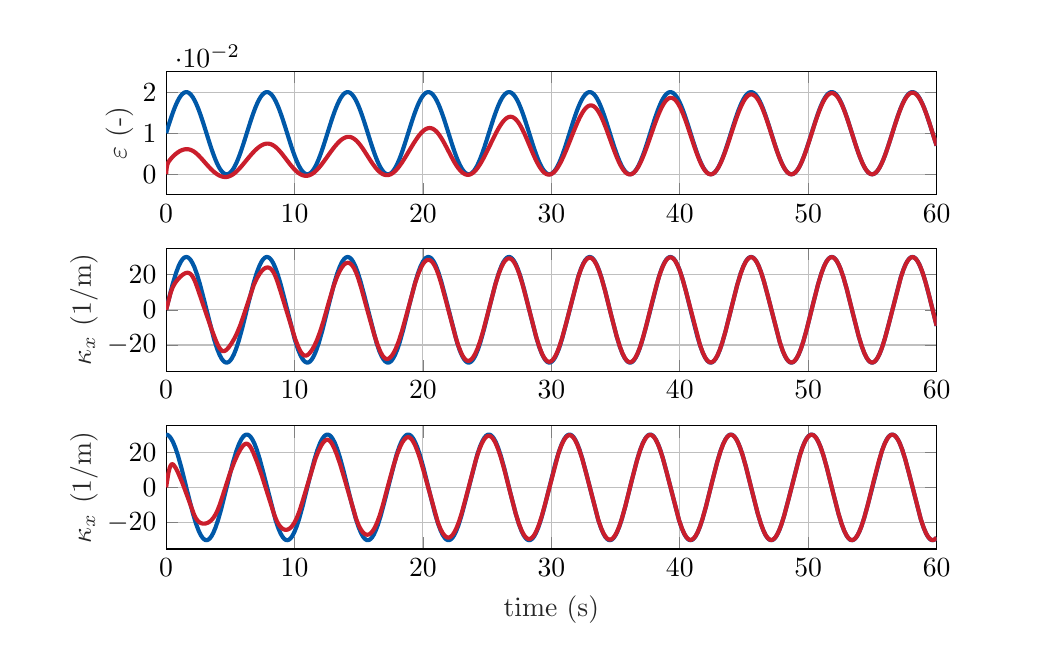
\begin{tikzpicture}

\begin{axis}[%
width=0.807\textwidth,
height=0.129\textwidth,
at={(0\textwidth,0.371\textwidth)},
scale only axis,
xmin=0,
xmax=60,
ymin=-0.005,
ymax=0.025,
ylabel style={font=\color{white!15!black}},
ylabel={$\varepsilon$ (-)},
axis background/.style={fill=white},
xmajorgrids,
ymajorgrids,
ylabel style={yshift=-3.5pt}
]
\addplot [color=mycolor1, line width=1.5pt, forget plot]
  table[row sep=crcr]{%
0	0.00999999999999801\\
0.175069999999998	0.0117419999999981\\
0.275109999999998	0.0127170000000021\\
0.375160000000001	0.0136639999999986\\
0.450189999999999	0.0143509999999978\\
0.525219999999997	0.0150140000000007\\
0.600250000000003	0.0156479999999988\\
0.650269999999999	0.0160539999999969\\
0.725299999999997	0.0166340000000034\\
0.775320000000001	0.0169989999999984\\
0.825339999999997	0.0173479999999984\\
0.875360000000001	0.0176779999999965\\
0.92539	0.017989\\
0.975409999999997	0.0182789999999997\\
1.0254	0.0185490000000001\\
1.0754	0.0187979999999968\\
1.1255	0.0190249999999992\\
1.1755	0.0192290000000028\\
1.2255	0.0194100000000006\\
1.2755	0.0195670000000021\\
1.3256	0.0197009999999977\\
1.3756	0.0198099999999997\\
1.4256	0.0198949999999982\\
1.4756	0.0199550000000031\\
1.5256	0.01999\\
1.5757	0.0200000000000031\\
1.6257	0.0199849999999984\\
1.6757	0.0199449999999999\\
1.7257	0.0198800000000006\\
1.7757	0.0197909999999979\\
1.8258	0.0196770000000015\\
1.8758	0.0195390000000017\\
1.9258	0.0193760000000012\\
1.9758	0.0191909999999993\\
2.0258	0.0189820000000012\\
2.0759	0.0187510000000017\\
2.1259	0.0184989999999985\\
2.1759	0.0182239999999965\\
2.2259	0.0179299999999998\\
2.2759	0.0176149999999993\\
2.326	0.0172820000000016\\
2.376	0.0169300000000021\\
2.451	0.016370000000002\\
2.5261	0.0157740000000004\\
2.6011	0.0151460000000014\\
2.6761	0.0144880000000001\\
2.7511	0.0138060000000024\\
2.8262	0.0131020000000035\\
2.9262	0.0121370000000027\\
3.0513	0.0109020000000015\\
3.3764	0.00767340000000161\\
3.4764	0.00671369999999882\\
3.5765	0.00578680000000276\\
3.6515	0.0051187999999982\\
3.7266	0.00447830000000238\\
3.8016	0.00386890000000051\\
3.8516	0.00348160000000064\\
3.9016	0.00311049999999824\\
3.9516	0.00275680000000023\\
4.0017	0.0024210999999994\\
4.0517	0.00210440000000034\\
4.1017	0.00180739999999702\\
4.1517	0.00153099999999995\\
4.2018	0.00127570000000077\\
4.2518	0.00104220000000055\\
4.3018	0.000831169999997883\\
4.3518	0.000643060000001583\\
4.4018	0.000478360000002453\\
4.4519	0.000337469999998063\\
4.5019	0.000220759999997711\\
4.5519	0.000128510000003246\\
4.6019	6.09579999988341e-05\\
4.6519	1.82659999978796e-05\\
4.702	5.43900000593567e-07\\
4.752	7.83619999822349e-06\\
4.802	4.01249999981701e-05\\
4.852	9.73280000025056e-05\\
4.902	0.000179299999999216\\
4.9521	0.000285849999997367\\
5.0021	0.000416690000001552\\
5.0521	0.00057151000000033\\
5.1021	0.00074991000000324\\
5.1521	0.000951450000002296\\
5.2022	0.00117560000000339\\
5.2522	0.00142189999999687\\
5.3022	0.00168959999999885\\
5.3522	0.00197810000000231\\
5.4023	0.00228669999999909\\
5.4523	0.00261449999999996\\
5.5023	0.00296089999999793\\
5.5523	0.00332480000000146\\
5.6023	0.00370550000000236\\
5.6774	0.00430560000000213\\
5.7524	0.0049379000000016\\
5.8274	0.00559859999999901\\
5.9025	0.00628410000000201\\
5.9775	0.0069903999999994\\
6.0775	0.00795790000000096\\
6.2026	0.00919489999999712\\
6.4777	0.0119329999999991\\
6.5777	0.0129030000000014\\
6.6528	0.013612000000002\\
6.7278	0.0143010000000032\\
6.8028	0.0149660000000011\\
6.8779	0.0156020000000012\\
6.9279	0.0160100000000014\\
6.9779	0.0164019999999994\\
7.0279	0.0167780000000022\\
7.0779	0.0171369999999982\\
7.128	0.017477999999997\\
7.178	0.0178009999999986\\
7.228	0.018104000000001\\
7.278	0.018386999999997\\
7.3281	0.0186490000000035\\
7.3781	0.0188890000000015\\
7.4281	0.0191069999999982\\
7.4781	0.0193020000000033\\
7.5281	0.0194740000000024\\
7.5782	0.0196219999999983\\
7.6282	0.0197459999999978\\
7.6782	0.0198460000000011\\
7.7282	0.0199209999999965\\
7.7782	0.0199709999999982\\
7.8283	0.0199969999999965\\
7.8783	0.0199969999999965\\
7.9283	0.0199720000000028\\
7.9783	0.0199229999999986\\
8.0283	0.0198480000000032\\
8.0784	0.0197489999999974\\
8.1284	0.0196260000000024\\
8.1784	0.0194779999999994\\
8.2284	0.0193069999999977\\
8.2784	0.0191129999999973\\
8.3285	0.0188950000000006\\
8.3785	0.018656\\
8.4285	0.0183940000000007\\
8.4785	0.0181120000000021\\
8.5286	0.0178099999999972\\
8.5786	0.0174880000000002\\
8.6286	0.0171470000000014\\
8.6786	0.0167879999999982\\
8.7536	0.0162189999999995\\
8.8037	0.0158190000000005\\
8.8787	0.0151929999999965\\
8.9537	0.0145380000000017\\
9.0288	0.0138570000000016\\
9.1038	0.0131549999999976\\
9.1788	0.0124350000000035\\
9.3039	0.0112060000000014\\
9.654	0.00772760000000261\\
9.7541	0.00676630000000245\\
9.8291	0.00606609999999819\\
9.9041	0.0053880000000035\\
9.9792	0.00473579999999885\\
10.029	0.00431729999999675\\
10.104	0.00371650000000301\\
10.154	0.00333539999999743\\
10.204	0.00297090000000111\\
10.254	0.00262409999999846\\
10.304	0.00229569999999768\\
10.354	0.00198660000000217\\
10.404	0.0016974999999988\\
10.454	0.00142919999999691\\
10.504	0.00118230000000352\\
10.554	0.00095749999999839\\
10.604	0.000755310000002396\\
10.654	0.000576240000000894\\
10.704	0.000420750000003522\\
10.754	0.000289219999999091\\
10.805	0.00018199000000152\\
10.855	9.93129999997677e-05\\
10.905	4.14040000009663e-05\\
10.955	8.40789999756453e-06\\
11.005	4.0598000339287e-07\\
11.055	1.74190000024055e-05\\
11.105	5.94030000016232e-05\\
11.155	0.000126260000001821\\
11.205	0.000217810000002316\\
11.255	0.000333830000002422\\
11.305	0.000474029999999459\\
11.355	0.000638059999999996\\
11.405	0.000825519999999358\\
11.455	0.00103589999999798\\
11.505	0.00126869999999712\\
11.555	0.00152340000000351\\
11.605	0.00179930000000184\\
11.655	0.00209569999999815\\
11.705	0.0024117999999973\\
11.755	0.00274699999999939\\
11.805	0.00310029999999983\\
11.855	0.00347080000000233\\
11.905	0.00385769999999752\\
11.98	0.00446649999999948\\
12.055	0.00510649999999657\\
12.13	0.00577400000000239\\
12.205	0.00646520000000095\\
12.28	0.00717639999999875\\
12.38	0.0081485999999984\\
12.505	0.00938880000000353\\
12.755	0.0118780000000029\\
12.855	0.0128500000000003\\
12.93	0.0135599999999982\\
13.005	0.0142510000000016\\
13.08	0.014916999999997\\
13.13	0.0153469999999984\\
13.18	0.0157620000000023\\
13.306	0.0167369999999991\\
13.381	0.0172719999999984\\
13.431	0.0176060000000007\\
13.481	0.0179210000000012\\
13.531	0.0182160000000025\\
13.581	0.0184909999999974\\
13.631	0.0187450000000027\\
13.681	0.0189760000000021\\
13.731	0.0191850000000002\\
13.781	0.0193719999999971\\
13.831	0.0195340000000002\\
13.881	0.0196729999999974\\
13.931	0.0197879999999984\\
13.981	0.0198779999999985\\
14.031	0.0199440000000024\\
14.081	0.0199840000000009\\
14.131	0.0200000000000031\\
14.181	0.01999\\
14.231	0.0199560000000005\\
14.281	0.0198970000000003\\
14.331	0.0198129999999992\\
14.381	0.0197039999999973\\
14.431	0.0195709999999991\\
14.481	0.0194150000000022\\
14.531	0.0192339999999973\\
14.581	0.0190309999999982\\
14.631	0.0188050000000004\\
14.681	0.0185570000000013\\
14.731	0.0182870000000008\\
14.781	0.0179970000000012\\
14.831	0.0176870000000022\\
14.881	0.017356999999997\\
14.931	0.0170099999999991\\
14.981	0.0166439999999994\\
15.031	0.0162619999999976\\
15.106	0.0156599999999969\\
15.181	0.0150259999999989\\
15.256	0.0143640000000005\\
15.331	0.0136770000000013\\
15.406	0.0129700000000028\\
15.506	0.0120009999999979\\
15.657	0.0105140000000006\\
15.882	0.0082722000000004\\
15.982	0.00729710000000239\\
16.057	0.00658299999999912\\
16.132	0.00588809999999995\\
16.207	0.0052164000000019\\
16.282	0.00457159999999845\\
16.357	0.00395730000000327\\
16.407	0.00356639999999686\\
16.457	0.00319170000000213\\
16.507	0.002834\\
16.557	0.002494200000001\\
16.607	0.00217320000000143\\
16.657	0.00187180000000353\\
16.707	0.00159070000000128\\
16.757	0.00133069999999691\\
16.807	0.00109230000000338\\
16.857	0.000876200000000438\\
16.907	0.000682939999997245\\
16.957	0.00051298999999716\\
17.007	0.000366769999999406\\
17.057	0.000244649999999069\\
17.107	0.000146929999999657\\
17.157	7.38549999965699e-05\\
17.207	2.56149999984245e-05\\
17.257	2.32600000060756e-06\\
17.307	4.04720000091174e-06\\
17.357	3.07740000025092e-05\\
17.407	8.24390000033759e-05\\
17.457	0.000158910000003232\\
17.507	0.00026000999999809\\
17.557	0.00038545999999684\\
17.607	0.000534969999996804\\
17.657	0.000708160000002067\\
17.707	0.00090458999999754\\
17.757	0.00112380000000201\\
17.807	0.00136520000000218\\
17.857	0.00162819999999897\\
17.907	0.00191209999999842\\
17.957	0.00221619999999945\\
18.033	0.00270880000000062\\
18.083	0.00306009999999901\\
18.133	0.00342870000000062\\
18.183	0.0038138000000032\\
18.258	0.00442019999999843\\
18.333	0.00505799999999823\\
18.408	0.00572350000000199\\
18.483	0.00641319999999723\\
18.558	0.00712299999999999\\
18.658	0.00809389999999865\\
18.783	0.00933320000000037\\
19.058	0.0120689999999968\\
19.158	0.0130359999999996\\
19.233	0.0137410000000031\\
19.308	0.0144260000000003\\
19.383	0.0150859999999966\\
19.458	0.0157170000000022\\
19.533	0.0163160000000033\\
19.583	0.0166960000000032\\
19.633	0.0170590000000033\\
19.708	0.0175699999999992\\
19.758	0.0178870000000018\\
19.808	0.018183999999998\\
19.858	0.0184610000000021\\
19.908	0.0187170000000023\\
19.958	0.0189510000000013\\
20.008	0.0191629999999989\\
20.058	0.0193519999999978\\
20.108	0.0195170000000005\\
20.158	0.0196589999999972\\
20.208	0.0197760000000002\\
20.258	0.0198689999999999\\
20.308	0.0199369999999988\\
20.358	0.0199810000000014\\
20.409	0.0199989999999985\\
20.459	0.0199929999999995\\
20.509	0.0199610000000021\\
20.559	0.0199050000000014\\
20.609	0.0198230000000024\\
20.659	0.0197179999999975\\
20.709	0.0195870000000014\\
20.759	0.0194329999999994\\
20.809	0.0192550000000011\\
20.859	0.0190550000000016\\
20.909	0.0188309999999987\\
20.959	0.0185850000000016\\
21.009	0.0183180000000007\\
21.059	0.0180300000000031\\
21.109	0.0177219999999991\\
21.159	0.0173950000000005\\
21.209	0.0170490000000001\\
21.259	0.016686\\
21.309	0.0163060000000002\\
21.384	0.0157060000000016\\
21.459	0.0150739999999985\\
21.534	0.0144140000000021\\
21.609	0.0137289999999979\\
21.684	0.0130229999999969\\
21.784	0.0120560000000012\\
21.884	0.0110680000000016\\
22.234	0.00759269999999646\\
22.334	0.0066354000000004\\
22.409	0.00593889999999675\\
22.484	0.00526539999999898\\
22.559	0.00461839999999825\\
22.634	0.00400170000000344\\
22.684	0.00360919999999965\\
22.734	0.00323259999999692\\
22.784	0.00287300000000101\\
22.885	0.0022080000000031\\
22.935	0.00190440000000081\\
22.985	0.00162100000000009\\
23.035	0.00135850000000204\\
23.085	0.00111770000000178\\
23.135	0.000899140000001353\\
23.185	0.000703319999999508\\
23.235	0.000530750000002911\\
23.285	0.000381859999997403\\
23.335	0.000257040000001041\\
23.385	0.000156590000003121\\
23.435	8.07649999998716e-05\\
23.485	2.97529999997437e-05\\
23.535	3.68229999736513e-06\\
23.585	2.61779999988221e-06\\
23.635	2.65620000021727e-05\\
23.685	7.54559999975868e-05\\
23.735	0.000149180000001081\\
23.785	0.000247539999996604\\
23.835	0.000370300000000157\\
23.885	0.000517150000000299\\
23.935	0.000687720000001946\\
23.985	0.000881589999998766\\
24.035	0.00109830000000244\\
24.085	0.00133720000000181\\
24.135	0.00159779999999898\\
24.185	0.00187950000000114\\
24.235	0.00218139999999778\\
24.285	0.00250290000000319\\
24.335	0.00284320000000093\\
24.385	0.00320130000000063\\
24.435	0.0035765000000012\\
24.485	0.00396769999999691\\
24.56	0.0045825999999991\\
24.635	0.00522790000000128\\
24.71	0.00590009999999808\\
24.785	0.00659530000000075\\
24.86	0.00730970000000042\\
24.96	0.00828510000000193\\
25.11	0.00977720000000204\\
25.236	0.0110260000000011\\
25.361	0.0122590000000002\\
25.461	0.0132199999999969\\
25.536	0.0139210000000034\\
25.611	0.0145989999999969\\
25.686	0.0152519999999967\\
25.761	0.0158750000000012\\
25.811	0.0162720000000007\\
25.861	0.0166540000000026\\
25.911	0.0170189999999977\\
25.961	0.0173660000000027\\
26.011	0.0176950000000033\\
26.061	0.0180050000000023\\
26.111	0.0182950000000019\\
26.161	0.0185630000000003\\
26.211	0.0188109999999995\\
26.261	0.0190359999999998\\
26.311	0.0192389999999989\\
26.361	0.0194189999999992\\
26.411	0.0195750000000032\\
26.461	0.0197069999999968\\
26.511	0.0198150000000012\\
26.561	0.0198990000000023\\
26.611	0.019956999999998\\
26.661	0.0199909999999974\\
26.711	0.0200000000000031\\
26.761	0.0199830000000034\\
26.811	0.0199420000000003\\
26.861	0.0198759999999965\\
26.911	0.0197849999999988\\
26.961	0.0196699999999979\\
27.011	0.0195300000000032\\
27.061	0.0193670000000026\\
27.111	0.0191799999999986\\
27.161	0.018970000000003\\
27.211	0.018737999999999\\
27.261	0.0184840000000008\\
27.311	0.0182089999999988\\
27.361	0.0179130000000001\\
27.411	0.0175970000000021\\
27.461	0.0172629999999998\\
27.511	0.0169100000000029\\
27.561	0.0165399999999991\\
27.637	0.0159540000000007\\
27.687	0.015545000000003\\
27.762	0.0149060000000034\\
27.837	0.0142390000000034\\
27.912	0.0135480000000001\\
28.012	0.0125969999999995\\
28.137	0.0113720000000015\\
28.312	0.00962549999999851\\
28.462	0.00813569999999686\\
28.562	0.00716380000000072\\
28.637	0.00645300000000049\\
28.712	0.00576209999999833\\
28.787	0.00509499999999719\\
28.862	0.0044556\\
28.937	0.00384729999999678\\
28.987	0.00346090000000032\\
29.037	0.0030908000000025\\
29.087	0.00273789999999963\\
29.137	0.00240329999999744\\
29.187	0.00208760000000296\\
29.237	0.00179179999999945\\
29.287	0.00151650000000103\\
29.337	0.00126240000000166\\
29.387	0.00103010000000126\\
29.437	0.000820300000000884\\
29.487	0.000633460000003083\\
29.537	0.000470049999997002\\
29.587	0.000330470000001526\\
29.637	0.000215089999997531\\
29.687	0.000124180000000251\\
29.737	5.79829999978188e-05\\
29.787	1.66530000029752e-05\\
29.837	2.96289996981614e-07\\
29.887	8.95480000195903e-06\\
29.937	4.26069999974743e-05\\
29.987	0.00010117000000065\\
30.038	0.000184490000002313\\
30.088	0.000292369999996822\\
30.138	0.000424529999996537\\
30.188	0.000580650000003402\\
30.238	0.000760319999997705\\
30.288	0.000963120000001538\\
30.338	0.00118849999999782\\
30.388	0.00143599999999822\\
30.438	0.00170479999999884\\
30.488	0.00199440000000095\\
30.538	0.00230410000000347\\
30.588	0.00263300000000299\\
30.638	0.00298029999999727\\
30.688	0.00334519999999827\\
30.738	0.00372670000000141\\
30.788	0.00412390000000329\\
30.863	0.00474700000000183\\
30.938	0.00539959999999695\\
31.013	0.00607819999999748\\
31.088	0.00677879999999931\\
31.188	0.00774040000000298\\
31.313	0.00897299999999746\\
31.638	0.012203999999997\\
31.713	0.0129289999999997\\
31.813	0.0138699999999972\\
31.888	0.0145499999999998\\
31.963	0.0152050000000017\\
32.038	0.0158300000000011\\
32.113	0.0164230000000032\\
32.188	0.0169789999999992\\
32.238	0.0173289999999966\\
32.288	0.0176599999999993\\
32.338	0.0179710000000028\\
32.388	0.0182629999999975\\
32.464	0.0186619999999991\\
32.514	0.0189009999999996\\
32.564	0.0191179999999989\\
32.614	0.0193119999999993\\
32.664	0.019483000000001\\
32.714	0.0196290000000019\\
32.764	0.0197519999999969\\
32.814	0.0198510000000027\\
32.864	0.0199240000000032\\
32.914	0.0199730000000002\\
32.964	0.0199969999999965\\
33.014	0.019995999999999\\
33.064	0.0199700000000007\\
33.114	0.0199190000000016\\
33.164	0.0198439999999991\\
33.214	0.0197429999999983\\
33.264	0.0196180000000012\\
33.314	0.0194699999999983\\
33.364	0.0192970000000017\\
33.414	0.0191009999999991\\
33.464	0.0188830000000024\\
33.514	0.0186419999999998\\
33.564	0.0183800000000005\\
33.614	0.0180959999999999\\
33.664	0.0177929999999975\\
33.714	0.017470000000003\\
33.764	0.0171279999999996\\
33.814	0.016767999999999\\
33.864	0.0163920000000033\\
33.939	0.0157969999999992\\
33.989	0.0153820000000024\\
34.064	0.0147359999999992\\
34.139	0.0140620000000027\\
34.214	0.0133659999999978\\
34.314	0.0124080000000006\\
34.414	0.0114269999999976\\
34.589	0.00968110000000166\\
34.739	0.00819049999999777\\
34.789	0.00770099999999729\\
34.84	0.00721730000000065\\
34.915	0.00650509999999827\\
34.99	0.00581259999999872\\
35.065	0.0051435999999967\\
35.14	0.00450200000000223\\
35.215	0.00389129999999938\\
35.265	0.0035031000000032\\
35.315	0.00313109999999739\\
35.365	0.0027764000000019\\
35.415	0.00243960000000243\\
35.465	0.00212179999999762\\
35.515	0.00182370000000276\\
35.565	0.00154609999999877\\
35.615	0.00128959999999978\\
35.665	0.00105489999999975\\
35.715	0.000842540000000724\\
35.765	0.000653110000001789\\
35.815	0.000487069999998369\\
35.865	0.000344820000002244\\
35.915	0.000226730000001396\\
35.965	0.000133089999998504\\
36.015	6.41259999980548e-05\\
36.065	2.00200000008977e-05\\
36.115	8.80130002656188e-07\\
36.165	6.75329999921814e-06\\
36.215	3.76249999973766e-05\\
36.265	9.3417999998735e-05\\
36.315	0.000173990000000401\\
36.365	0.00027914999999723\\
36.415	0.000408620000001747\\
36.465	0.000562090000002513\\
36.515	0.000739160000001959\\
36.565	0.000939410000000862\\
36.615	0.00116229999999717\\
36.665	0.00140729999999678\\
36.715	0.00167379999999895\\
36.765	0.00196119999999667\\
36.815	0.00226860000000073\\
36.865	0.00259539999999703\\
36.915	0.00294070000000346\\
36.965	0.00330369999999647\\
37.015	0.00368339999999989\\
37.09	0.00428229999999985\\
37.165	0.00491339999999951\\
37.266	0.00579869999999971\\
37.341	0.00649080000000168\\
37.416	0.00720259999999939\\
37.516	0.00817550000000011\\
37.641	0.00941610000000281\\
37.891	0.0119049999999987\\
37.991	0.0128759999999986\\
38.066	0.0135859999999965\\
38.141	0.0142749999999978\\
38.216	0.0149410000000003\\
38.291	0.0155790000000025\\
38.341	0.0159870000000026\\
38.416	0.0165700000000015\\
38.466	0.0169390000000007\\
38.516	0.0172910000000002\\
38.566	0.0176239999999979\\
38.616	0.0179380000000009\\
38.666	0.0182319999999976\\
38.716	0.0185049999999976\\
38.766	0.0187579999999983\\
38.816	0.0189880000000002\\
38.866	0.0191960000000009\\
38.916	0.0193810000000028\\
38.966	0.0195420000000013\\
39.016	0.019680000000001\\
39.066	0.0197929999999999\\
39.116	0.0198820000000026\\
39.166	0.0199459999999974\\
39.216	0.0199860000000029\\
39.266	0.0200000000000031\\
39.316	0.0199890000000025\\
39.366	0.019953000000001\\
39.416	0.0198930000000033\\
39.466	0.0198070000000001\\
39.516	0.0196979999999982\\
39.566	0.019562999999998\\
39.617	0.019404999999999\\
39.667	0.0192240000000012\\
39.717	0.0190190000000001\\
39.767	0.0187919999999977\\
39.817	0.0185430000000011\\
39.867	0.0182720000000032\\
39.917	0.0179809999999989\\
39.967	0.0176689999999979\\
40.017	0.0173389999999998\\
40.067	0.0169899999999998\\
40.117	0.0166240000000002\\
40.192	0.0160440000000008\\
40.267	0.0154289999999975\\
40.342	0.0147850000000034\\
40.417	0.0141130000000018\\
40.492	0.0134180000000015\\
40.567	0.0127039999999994\\
40.667	0.0117290000000025\\
40.817	0.0102369999999965\\
41.017	0.00824529999999868\\
41.117	0.00727080000000058\\
41.192	0.00655729999999721\\
41.267	0.00586320000000029\\
41.342	0.00519239999999854\\
41.417	0.00454859999999968\\
41.492	0.00393549999999721\\
41.542	0.00354560000000248\\
41.592	0.00317170000000289\\
41.642	0.00281499999999824\\
41.692	0.00247619999999671\\
41.742	0.00215620000000172\\
41.792	0.00185590000000246\\
41.842	0.00157600000000002\\
41.892	0.0013171000000014\\
41.942	0.00107990000000058\\
41.992	0.000865050000001588\\
42.068	0.000585780000001535\\
42.118	0.000428939999999045\\
42.168	0.000296040000002051\\
42.218	0.000187420000003158\\
42.268	0.000103340000002561\\
42.318	4.40239999974779e-05\\
42.368	9.61149999767485e-06\\
42.418	1.90539999778139e-07\\
42.468	1.57850000022108e-05\\
42.518	5.63549999981205e-05\\
42.568	0.000121800000002281\\
42.618	0.000211960000001454\\
42.668	0.000326600000001065\\
42.718	0.000465439999999262\\
42.768	0.000628130000002614\\
42.818	0.000814259999998512\\
42.868	0.00102340000000112\\
42.918	0.00125489999999928\\
42.968	0.00150839999999874\\
43.018	0.00178309999999726\\
43.068	0.00207830000000087\\
43.118	0.00239340000000254\\
43.168	0.00272749999999888\\
43.218	0.00307980000000185\\
43.268	0.00344929999999977\\
43.318	0.00383529999999865\\
43.393	0.0044429000000008\\
43.468	0.00508169999999808\\
43.543	0.00574830000000048\\
43.618	0.0064386999999968\\
43.693	0.00714920000000063\\
43.793	0.0081206999999992\\
43.918	0.00936049999999966\\
44.193	0.0120959999999997\\
44.293	0.0130619999999979\\
44.368	0.0137670000000014\\
44.419	0.0142250000000033\\
44.494	0.0148930000000007\\
44.569	0.0155329999999978\\
44.644	0.0161409999999975\\
44.694	0.016528000000001\\
44.744	0.0168990000000022\\
44.794	0.0172519999999992\\
44.844	0.0175869999999989\\
44.894	0.0179040000000015\\
44.944	0.0182000000000002\\
44.994	0.0184759999999997\\
45.044	0.0187310000000025\\
45.094	0.0189639999999969\\
45.144	0.0191739999999996\\
45.194	0.019362000000001\\
45.244	0.019525999999999\\
45.294	0.0196660000000008\\
45.344	0.0197819999999993\\
45.394	0.0198740000000015\\
45.444	0.0199399999999983\\
45.494	0.0199830000000034\\
45.544	0.0200000000000031\\
45.594	0.019992000000002\\
45.644	0.0199590000000001\\
45.694	0.0199009999999973\\
45.744	0.0198180000000008\\
45.794	0.0197110000000009\\
45.844	0.0195799999999977\\
45.894	0.0194240000000008\\
45.944	0.019244999999998\\
45.994	0.0190430000000035\\
46.044	0.0188180000000031\\
46.094	0.0185710000000014\\
46.144	0.0183030000000031\\
46.194	0.0180140000000009\\
46.244	0.0177049999999994\\
46.294	0.0173770000000033\\
46.369	0.016849999999998\\
46.444	0.0162839999999989\\
46.494	0.0158879999999968\\
46.569	0.0152649999999994\\
46.644	0.0146129999999971\\
46.719	0.0139349999999965\\
46.82	0.0129969999999986\\
46.895	0.0122730000000004\\
46.995	0.0112889999999979\\
47.17	0.00954250000000201\\
47.32	0.00805419999999657\\
47.42	0.00708430000000249\\
47.495	0.0063754999999972\\
47.57	0.00568700000000177\\
47.645	0.00502290000000016\\
47.72	0.00438669999999775\\
47.795	0.00378210000000223\\
47.845	0.00339830000000063\\
47.895	0.00303100000000001\\
47.945	0.00268109999999666\\
47.995	0.00234960000000228\\
48.045	0.00203710000000257\\
48.095	0.00174460000000209\\
48.145	0.00147280000000194\\
48.195	0.00122230000000201\\
48.245	0.000993719999996756\\
48.295	0.000787690000002783\\
48.345	0.000604699999996683\\
48.395	0.000445220000003133\\
48.445	0.000309639999997557\\
48.495	0.000198300000000984\\
48.545	0.000111480000001052\\
48.595	4.93989999981181e-05\\
48.645	1.22080000011238e-05\\
48.695	1.82149761940309e-09\\
48.745	1.28109999977255e-05\\
48.795	5.0604999998427e-05\\
48.845	0.000113290000001598\\
48.895	0.000200700000000609\\
48.945	0.000312630000003367\\
48.995	0.000448790000000088\\
49.045	0.000608849999998995\\
49.095	0.000792390000000864\\
49.145	0.000998969999997712\\
49.195	0.00122809999999873\\
49.246	0.0014790999999974\\
49.296	0.00175149999999746\\
49.346	0.00204449999999667\\
49.396	0.0023572999999999\\
49.446	0.00268940000000129\\
49.496	0.0030397000000022\\
49.546	0.00340740000000039\\
49.596	0.00379159999999956\\
49.671	0.00439670000000092\\
49.746	0.00503330000000091\\
49.821	0.00569790000000125\\
49.896	0.00638670000000019\\
49.971	0.00709580000000187\\
50.071	0.00806610000000063\\
50.196	0.00930489999999651\\
50.471	0.0120410000000035\\
50.571	0.0130089999999967\\
50.671	0.0139459999999971\\
50.746	0.0146239999999977\\
50.821	0.0152750000000026\\
50.896	0.0158970000000025\\
50.971	0.0164860000000004\\
51.021	0.0168589999999966\\
51.096	0.0173849999999973\\
51.146	0.0177130000000005\\
51.196	0.0180209999999974\\
51.246	0.0183099999999996\\
51.296	0.018577999999998\\
51.346	0.0188240000000022\\
51.396	0.019047999999998\\
51.446	0.0192499999999995\\
51.496	0.0194279999999978\\
51.546	0.0195829999999972\\
51.596	0.0197140000000005\\
51.647	0.0198200000000028\\
51.697	0.0199029999999993\\
51.747	0.0199599999999975\\
51.797	0.019992000000002\\
51.847	0.0199989999999985\\
51.897	0.0199819999999988\\
51.947	0.0199390000000008\\
51.997	0.0198719999999994\\
52.047	0.0197789999999998\\
52.097	0.0196630000000013\\
52.147	0.019522000000002\\
52.197	0.0193569999999994\\
52.247	0.019168999999998\\
52.297	0.0189579999999978\\
52.347	0.0187250000000034\\
52.397	0.0184700000000007\\
52.447	0.0181929999999966\\
52.497	0.0178960000000004\\
52.547	0.0175800000000024\\
52.597	0.017243999999998\\
52.647	0.0168899999999965\\
52.697	0.0165190000000024\\
52.747	0.0161319999999989\\
52.822	0.0155230000000017\\
52.897	0.0148820000000001\\
52.972	0.0142140000000026\\
53.047	0.0135220000000018\\
53.122	0.0128109999999992\\
53.222	0.0118379999999974\\
53.347	0.0105980000000017\\
53.597	0.00810890000000342\\
53.697	0.00713760000000008\\
53.772	0.00642739999999975\\
53.847	0.00573729999999983\\
53.922	0.00507120000000327\\
53.997	0.00443289999999763\\
54.123	0.0034402\\
54.173	0.00307099999999849\\
54.223	0.00271920000000136\\
54.273	0.00238559999999666\\
54.323	0.00207100000000082\\
54.373	0.00177620000000189\\
54.423	0.00150200000000211\\
54.473	0.00124910000000256\\
54.523	0.00101810000000313\\
54.573	0.000809500000002572\\
54.623	0.000623920000002443\\
54.673	0.000461799999996515\\
54.723	0.000323539999996569\\
54.773	0.000209490000003143\\
54.823	0.000119929999996771\\
54.873	5.50820000029262e-05\\
54.923	1.51139999999828e-05\\
54.973	1.23310002209109e-07\\
55.023	1.01480000012089e-05\\
55.073	4.51630000029013e-05\\
55.123	0.000105079999997315\\
55.173	0.000189749999996991\\
55.223	0.000298960000002069\\
55.273	0.000432439999997314\\
55.323	0.000589849999997227\\
55.373	0.000770809999998789\\
55.423	0.000974849999998639\\
55.473	0.00120150000000052\\
55.523	0.00145009999999957\\
55.573	0.0017201\\
55.623	0.00201080000000076\\
55.673	0.00232150000000075\\
55.723	0.00265149999999892\\
55.773	0.00299979999999778\\
55.823	0.00336560000000219\\
55.873	0.00374800000000164\\
55.923	0.00414609999999982\\
55.998	0.00477029999999701\\
56.073	0.00542389999999671\\
56.148	0.00610329999999948\\
56.223	0.00680460000000238\\
56.323	0.00776700000000119\\
56.499	0.00949889999999698\\
56.724	0.0117410000000007\\
56.849	0.0129549999999981\\
56.924	0.0136630000000011\\
56.999	0.0143500000000003\\
57.074	0.0150130000000033\\
57.149	0.0156479999999988\\
57.224	0.0162499999999994\\
57.274	0.0166329999999988\\
57.324	0.0169989999999984\\
57.374	0.0173470000000009\\
57.424	0.0176769999999991\\
57.474	0.0179880000000026\\
57.524	0.0182789999999997\\
57.574	0.0185490000000001\\
57.624	0.0187979999999968\\
57.674	0.0190240000000017\\
57.724	0.0192279999999982\\
57.774	0.0194090000000031\\
57.824	0.0195670000000021\\
57.874	0.0197009999999977\\
57.924	0.0198099999999997\\
57.974	0.0198949999999982\\
58.024	0.0199550000000031\\
58.074	0.01999\\
58.124	0.0200000000000031\\
58.174	0.0199849999999984\\
58.224	0.0199449999999999\\
58.274	0.0198800000000006\\
58.324	0.0197909999999979\\
58.374	0.0196770000000015\\
58.424	0.0195390000000017\\
58.474	0.0193769999999986\\
58.524	0.0191909999999993\\
58.574	0.0189829999999986\\
58.624	0.0187519999999992\\
58.674	0.0184989999999985\\
58.724	0.018225000000001\\
58.774	0.0179299999999998\\
58.85	0.0174510000000012\\
58.9	0.0171089999999978\\
58.975	0.0165610000000029\\
59.025	0.0161760000000015\\
59.1	0.0155689999999993\\
59.175	0.0149309999999971\\
59.25	0.0142650000000017\\
59.325	0.013575000000003\\
59.425	0.0126240000000024\\
59.525	0.0116470000000035\\
59.675	0.010154\\
59.875	0.00816360000000316\\
59.975	0.00719099999999884\\
60	0.00695189999999712\\
};
\addplot [color=mycolor2, line width=1.5pt, forget plot]
  table[row sep=crcr]{%
0	0\\
0.0250100000000018	0.000948909999998193\\
0.050021000000001	0.00163409999999686\\
0.0750310000000027	0.00204109999999957\\
0.10004	0.00238650000000007\\
0.125050000000002	0.00258379999999647\\
0.150060000000003	0.00279369999999801\\
0.175069999999998	0.00291380000000174\\
0.20008	0.00306900000000354\\
0.225090000000002	0.00316200000000322\\
0.250100000000003	0.00329359999999923\\
0.275109999999998	0.00337760000000031\\
0.300130000000003	0.00349709999999703\\
0.325139999999998	0.00357809999999859\\
0.350149999999999	0.00368960000000129\\
0.375160000000001	0.00376909999999953\\
0.400170000000003	0.00387400000000326\\
0.425179999999997	0.00395180000000295\\
0.450189999999999	0.00405070000000052\\
0.475200000000001	0.00412639999999698\\
0.500210000000003	0.00421949999999782\\
0.525219999999997	0.00429270000000059\\
0.550229999999999	0.00438050000000345\\
0.575240000000001	0.00445090000000192\\
0.600250000000003	0.00453370000000319\\
0.675280000000001	0.00474390000000113\\
0.700290000000003	0.00481769999999671\\
0.900379999999998	0.00530359999999774\\
1.0504	0.00559839999999667\\
1.1755	0.00579450000000037\\
1.2505	0.0058928999999992\\
1.3506	0.0059944999999999\\
1.4506	0.00606359999999739\\
1.5506	0.00609879999999663\\
1.6507	0.00609899999999897\\
1.7257	0.00607500000000272\\
1.8008	0.00603160000000003\\
1.8758	0.00596639999999837\\
1.9508	0.00588110000000341\\
2.0258	0.00577400000000239\\
2.1009	0.00564669999999978\\
2.1759	0.00549850000000163\\
2.2509	0.0053313000000017\\
2.351	0.00507970000000313\\
2.451	0.00479920000000078\\
2.5511	0.00449429999999751\\
2.6761	0.00408610000000209\\
2.8262	0.00356899999999882\\
3.1263	0.00250049999999646\\
3.3014	0.00188990000000189\\
3.4264	0.00147290000000311\\
3.5515	0.00107930000000067\\
3.6515	0.000785180000001162\\
3.7516	0.000512530000001732\\
3.8516	0.000263740000001178\\
3.9516	4.08240000027149e-05\\
4.0517	-0.000154580000000237\\
4.1517	-0.000321120000002395\\
4.2268	-0.000426359999998738\\
4.3018	-0.000514170000002423\\
4.3768	-0.000583990000002643\\
4.4519	-0.000635199999997837\\
4.5269	-0.000667149999998173\\
4.6019	-0.000679249999997467\\
4.6769	-0.000670970000001603\\
4.752	-0.000641950000002112\\
4.827	-0.000592040000000793\\
4.902	-0.000521270000000129\\
4.9771	-0.000429910000001144\\
5.0521	-0.000318409999998437\\
5.1271	-0.000187369999999021\\
5.2022	-3.75819999973714e-05\\
5.2772	0.000130079999998145\\
5.3772	0.000379700000003425\\
5.4773	0.00065674999999743\\
5.5773	0.000958420000003457\\
5.6774	0.00128169999999983\\
5.8024	0.00171149999999898\\
5.9525	0.0022562999999991\\
6.1526	0.00301240000000291\\
6.4527	0.00415240000000239\\
6.6028	0.00470140000000185\\
6.7278	0.00513939999999735\\
6.8529	0.00555479999999875\\
6.9529	0.00586760000000197\\
7.0529	0.00616029999999768\\
7.153	0.00643000000000171\\
7.253	0.00667390000000267\\
7.3281	0.00683839999999947\\
7.4031	0.00698570000000132\\
7.4781	0.00711470000000247\\
7.5531	0.00722439999999835\\
7.6282	0.00731379999999859\\
7.7032	0.00738220000000211\\
7.7782	0.0074286999999984\\
7.8533	0.00745260000000059\\
7.9283	0.00745359999999806\\
8.0033	0.00743109999999803\\
8.0784	0.00738499999999931\\
8.1534	0.00731499999999841\\
8.2284	0.00722139999999882\\
8.3035	0.00710420000000056\\
8.3785	0.00696409999999759\\
8.4535	0.00680160000000285\\
8.5286	0.00661759999999845\\
8.6036	0.00641350000000074\\
8.6786	0.00619050000000243\\
8.7787	0.00586659999999739\\
8.8787	0.00551629999999648\\
8.9787	0.00514400000000137\\
9.1038	0.00465470000000323\\
9.2789	0.00394210000000328\\
9.579	0.00271169999999898\\
9.704	0.00221979999999888\\
9.8291	0.00175200000000331\\
9.9291	0.00140019999999907\\
10.029	0.00107220000000297\\
10.129	0.000771110000002295\\
10.204	0.000564779999997711\\
10.279	0.000376340000002529\\
10.354	0.000206779999999185\\
10.429	5.70099999990248e-05\\
10.504	-7.21549999980198e-05\\
10.579	-0.000179969999997809\\
10.654	-0.000265749999996956\\
10.729	-0.000328899999999521\\
10.805	-0.000368940000001317\\
10.88	-0.00038550000000015\\
10.955	-0.000378380000000789\\
11.03	-0.000347509999997442\\
11.105	-0.000292999999999211\\
11.18	-0.000215079999996703\\
11.255	-0.000114170000003355\\
11.33	9.21560000222144e-06\\
11.405	0.000154389999998727\\
11.48	0.000320539999997038\\
11.555	0.000506739999998729\\
11.63	0.000711959999996736\\
11.705	0.00093506999999704\\
11.805	0.00125830000000349\\
11.905	0.00160799999999739\\
12.005	0.00198110000000185\\
12.105	0.00237409999999727\\
12.23	0.00288799999999867\\
12.38	0.003528799999998\\
12.68	0.00484289999999987\\
12.855	0.00559979999999882\\
13.005	0.00622599999999807\\
13.13	0.00672339999999849\\
13.231	0.00710039999999879\\
13.331	0.00745500000000021\\
13.431	0.00778379999999856\\
13.531	0.00808339999999674\\
13.606	0.00828680000000048\\
13.681	0.00847060000000255\\
13.756	0.00863329999999962\\
13.831	0.008773699999999\\
13.906	0.00889049999999969\\
13.981	0.00898269999999712\\
14.056	0.00904919999999976\\
14.131	0.00908929999999941\\
14.206	0.00910209999999978\\
14.281	0.00908710000000212\\
14.356	0.00904400000000294\\
14.431	0.00897270000000105\\
14.506	0.00887310000000241\\
14.581	0.0087455000000034\\
14.656	0.00859049999999684\\
14.731	0.00840889999999916\\
14.806	0.00820170000000076\\
14.881	0.00797010000000142\\
14.956	0.00771579999999972\\
15.031	0.00744029999999896\\
15.106	0.00714550000000003\\
15.206	0.00672569999999695\\
15.306	0.0062800999999979\\
15.406	0.00581389999999971\\
15.556	0.00508820000000298\\
15.907	0.00337249999999756\\
16.032	0.00278660000000031\\
16.132	0.00233930000000271\\
16.232	0.00191619999999659\\
16.307	0.00161719999999832\\
16.382	0.00133610000000317\\
16.457	0.00107419999999792\\
16.532	0.000833020000001738\\
16.607	0.000613970000003405\\
16.682	0.000418230000001074\\
16.757	0.000246930000002976\\
16.832	0.000101049999997826\\
16.907	-1.85210000012148e-05\\
16.982	-0.000111029999999346\\
17.057	-0.000175890000001289\\
17.132	-0.000212679999997079\\
17.207	-0.000221179999996934\\
17.282	-0.000201359999998374\\
17.357	-0.00015335999999877\\
17.432	-7.74860000021249e-05\\
17.507	2.58009999996034e-05\\
17.582	0.000155919999997423\\
17.657	0.000312129999997524\\
17.732	0.000493599999998651\\
17.807	0.000699330000003329\\
17.882	0.000928199999997048\\
17.957	0.00117900000000049\\
18.058	0.0015451000000013\\
18.133	0.00184169999999995\\
18.233	0.00226359999999914\\
18.333	0.00271209999999655\\
18.433	0.00318349999999867\\
18.558	0.00379879999999844\\
18.708	0.00456510000000065\\
18.933	0.0057436000000024\\
19.158	0.00691770000000247\\
19.283	0.00755180000000166\\
19.408	0.00816269999999975\\
19.508	0.00862899999999911\\
19.608	0.00907089999999755\\
19.683	0.00938349999999843\\
19.758	0.00967800000000096\\
19.833	0.00995269999999948\\
19.908	0.0102059999999966\\
19.983	0.0104350000000011\\
20.058	0.0106389999999976\\
20.133	0.010817000000003\\
20.208	0.0109660000000034\\
20.283	0.0110850000000013\\
20.358	0.0111729999999994\\
20.409	0.0112140000000025\\
20.484	0.0112480000000019\\
20.534	0.0112519999999989\\
20.609	0.0112290000000002\\
20.684	0.0111709999999974\\
20.759	0.0110790000000023\\
20.809	0.0109980000000007\\
20.859	0.0109020000000015\\
20.934	0.0107300000000023\\
21.009	0.0105239999999966\\
21.084	0.0102860000000007\\
21.159	0.0100169999999977\\
21.234	0.00971990000000034\\
21.309	0.00939509999999899\\
21.384	0.00904529999999681\\
21.459	0.00867279999999937\\
21.534	0.00828010000000035\\
21.634	0.00772940000000233\\
21.734	0.00715399999999988\\
21.859	0.00641060000000238\\
22.259	0.00400779999999656\\
22.359	0.00343780000000038\\
22.459	0.00289279999999792\\
22.534	0.00250410000000301\\
22.609	0.00213509999999673\\
22.684	0.00178789999999651\\
22.759	0.00146449999999732\\
22.81	0.00126310000000274\\
22.885	0.000983300000001464\\
22.96	0.000731840000000261\\
23.035	0.000510099999999625\\
23.11	0.000319349999998053\\
23.185	0.000160690000001296\\
23.26	3.5064000002194e-05\\
23.31	-2.99619999992728e-05\\
23.36	-7.98009999982696e-05\\
23.41	-0.000114330000002383\\
23.46	-0.000133449999999868\\
23.51	-0.00013712999999882\\
23.56	-0.000125369999999236\\
23.61	-9.82190000016203e-05\\
23.66	-5.57520000015188e-05\\
23.71	1.90779999797996e-06\\
23.785	0.000116540000000498\\
23.86	0.000264330000000257\\
23.935	0.000444450000003371\\
24.01	0.000655899999998155\\
24.085	0.000897530000003144\\
24.16	0.00116799999999984\\
24.235	0.00146589999999946\\
24.31	0.00178970000000334\\
24.385	0.00213759999999752\\
24.46	0.00250779999999651\\
24.535	0.00289860000000175\\
24.61	0.00330790000000292\\
24.71	0.00387920000000008\\
24.81	0.00447530000000285\\
24.935	0.00524810000000286\\
25.085	0.0062035999999992\\
25.511	0.00894240000000224\\
25.636	0.00971779999999711\\
25.736	0.0103160000000031\\
25.836	0.0108880000000013\\
25.911	0.011296999999999\\
26.011	0.011809999999997\\
26.086	0.0121680000000026\\
26.161	0.0125010000000003\\
26.236	0.0128059999999977\\
26.311	0.0130809999999997\\
26.386	0.0133229999999998\\
26.461	0.0135310000000004\\
26.511	0.0136499999999984\\
26.561	0.0137519999999967\\
26.611	0.0138370000000023\\
26.661	0.0139039999999966\\
26.711	0.0139539999999982\\
26.761	0.0139849999999981\\
26.811	0.0139980000000008\\
26.861	0.0139920000000018\\
26.911	0.013967000000001\\
26.961	0.0139229999999984\\
27.011	0.0138600000000011\\
27.061	0.0137780000000021\\
27.111	0.0136770000000013\\
27.161	0.0135569999999987\\
27.211	0.013418999999999\\
27.261	0.0132619999999974\\
27.311	0.0130880000000033\\
27.361	0.0128959999999978\\
27.411	0.0126869999999997\\
27.486	0.0123430000000013\\
27.536	0.0120950000000022\\
27.612	0.0116950000000031\\
27.687	0.0112639999999971\\
27.762	0.0108060000000023\\
27.837	0.0103229999999996\\
27.912	0.0098179000000016\\
28.012	0.00911709999999744\\
28.112	0.00839229999999702\\
28.262	0.00727870000000053\\
28.487	0.00560689999999653\\
28.587	0.00488529999999798\\
28.687	0.0041883000000027\\
28.762	0.00368629999999825\\
28.837	0.00320549999999997\\
28.912	0.00274869999999794\\
28.987	0.00231850000000122\\
29.062	0.00191749999999757\\
29.137	0.00154799999999966\\
29.187	0.00132010000000093\\
29.237	0.0011076999999986\\
29.287	0.000911289999997678\\
29.337	0.000731399999999383\\
29.387	0.00056845000000294\\
29.437	0.000422870000001296\\
29.487	0.000295010000002094\\
29.537	0.000185209999997937\\
29.587	9.37430000007566e-05\\
29.637	2.08410000013259e-05\\
29.687	-3.33110000028114e-05\\
29.737	-6.85790000005682e-05\\
29.787	-8.48809999993705e-05\\
29.837	-8.21810000033452e-05\\
29.887	-6.04960000032406e-05\\
29.937	-1.98910000008823e-05\\
29.987	3.95240000017338e-05\\
30.038	0.00011759000000211\\
30.088	0.00021411000000171\\
30.138	0.000328840000001662\\
30.188	0.00046147999999846\\
30.238	0.000611720000001981\\
30.288	0.000779170000001272\\
30.338	0.000963419999997939\\
30.388	0.00116400000000283\\
30.438	0.00138050000000334\\
30.488	0.0016122999999979\\
30.563	0.00198759999999965\\
30.638	0.00239419999999768\\
30.713	0.00282980000000066\\
30.788	0.00329239999999942\\
30.863	0.0037793999999991\\
30.938	0.00428860000000242\\
31.013	0.0048174000000003\\
31.113	0.00554850000000329\\
31.213	0.00630400000000009\\
31.338	0.0072732000000002\\
31.538	0.00885279999999966\\
31.713	0.01023\\
31.838	0.0111899999999991\\
31.938	0.0119350000000011\\
32.013	0.012475000000002\\
32.088	0.0129960000000011\\
32.163	0.0134940000000014\\
32.238	0.0139679999999984\\
32.313	0.0144129999999976\\
32.388	0.0148280000000014\\
32.489	0.0153279999999967\\
32.539	0.0155540000000016\\
32.589	0.0157620000000023\\
32.639	0.0159519999999986\\
32.689	0.0161239999999978\\
32.739	0.0162759999999977\\
32.789	0.016409000000003\\
32.839	0.0165220000000019\\
32.889	0.0166129999999995\\
32.939	0.0166839999999979\\
32.989	0.0167330000000021\\
33.039	0.0167599999999979\\
33.089	0.016765999999997\\
33.139	0.0167489999999972\\
33.189	0.0167100000000033\\
33.239	0.016649000000001\\
33.289	0.0165659999999974\\
33.339	0.0164600000000021\\
33.389	0.016333000000003\\
33.439	0.0161850000000001\\
33.489	0.0160160000000005\\
33.539	0.0158249999999995\\
33.589	0.0156149999999968\\
33.639	0.015385000000002\\
33.689	0.0151350000000008\\
33.739	0.0148670000000024\\
33.789	0.0145819999999972\\
33.839	0.0142790000000019\\
33.889	0.0139610000000019\\
33.964	0.0134550000000004\\
34.039	0.0129170000000016\\
34.114	0.0123519999999999\\
34.189	0.0117619999999974\\
34.264	0.0111509999999981\\
34.364	0.010311999999999\\
34.489	0.00923360000000173\\
34.789	0.00662530000000316\\
34.84	0.00620090000000317\\
34.94	0.00537140000000136\\
35.015	0.00477039999999818\\
35.09	0.0041916999999998\\
35.165	0.00363850000000099\\
35.24	0.00311419999999885\\
35.315	0.00262180000000001\\
35.365	0.00231269999999739\\
35.415	0.00201990000000052\\
35.465	0.00174400000000219\\
35.515	0.00148579999999754\\
35.565	0.00124600000000186\\
35.615	0.00102509999999967\\
35.665	0.00082366000000178\\
35.715	0.000642290000001822\\
35.765	0.000481389999997361\\
35.815	0.000341380000001834\\
35.865	0.000222600000000739\\
35.915	0.000125349999997582\\
35.965	4.98879999994983e-05\\
36.015	-3.60509999808301e-06\\
36.065	-3.49970000002031e-05\\
36.115	-4.42110000022922e-05\\
36.165	-3.12310000012417e-05\\
36.215	3.90710000175432e-06\\
36.265	6.11090000006698e-05\\
36.315	0.000140229999999519\\
36.365	0.000241060000000459\\
36.415	0.000363350000000651\\
36.465	0.000506799999996588\\
36.515	0.000671040000000289\\
36.565	0.000855669999999975\\
36.615	0.00106019999999774\\
36.665	0.00128420000000062\\
36.715	0.00152700000000294\\
36.765	0.00178809999999885\\
36.815	0.00206690000000265\\
36.865	0.00236249999999671\\
36.915	0.00267439999999652\\
36.99	0.00317100000000181\\
37.065	0.00369969999999853\\
37.14	0.00425769999999659\\
37.241	0.00504209999999716\\
37.316	0.00565660000000179\\
37.391	0.00629020000000224\\
37.491	0.00715900000000147\\
37.616	0.00827230000000156\\
38.016	0.0118640000000028\\
38.116	0.0127269999999982\\
38.191	0.0133539999999996\\
38.266	0.0139599999999973\\
38.341	0.0145430000000033\\
38.416	0.0150980000000018\\
38.491	0.0156220000000005\\
38.541	0.0159530000000032\\
38.591	0.0162690000000012\\
38.641	0.016567000000002\\
38.691	0.0168480000000031\\
38.741	0.0171100000000024\\
38.791	0.0173539999999974\\
38.841	0.0175770000000028\\
38.891	0.0177809999999994\\
38.941	0.0179630000000017\\
38.991	0.0181230000000028\\
39.041	0.018262\\
39.091	0.0183779999999985\\
39.141	0.0184709999999981\\
39.191	0.018540999999999\\
39.241	0.0185880000000012\\
39.291	0.0186109999999999\\
39.341	0.0186100000000025\\
39.391	0.0185859999999991\\
39.441	0.0185379999999995\\
39.491	0.0184659999999965\\
39.541	0.0183699999999973\\
39.591	0.0182519999999968\\
39.642	0.0181100000000001\\
39.692	0.017946000000002\\
39.742	0.0177589999999981\\
39.792	0.01755\\
39.842	0.0173210000000026\\
39.892	0.0170699999999968\\
39.942	0.0167989999999989\\
39.992	0.0165089999999992\\
40.042	0.0161999999999978\\
40.092	0.0158739999999966\\
40.142	0.0155299999999983\\
40.192	0.0151699999999977\\
40.267	0.0146019999999965\\
40.342	0.0140019999999978\\
40.417	0.0133760000000009\\
40.492	0.0127250000000032\\
40.567	0.0120539999999991\\
40.667	0.0111360000000005\\
40.792	0.00996159999999691\\
41.067	0.00736739999999969\\
41.167	0.00645099999999843\\
41.242	0.00578269999999748\\
41.317	0.00513490000000161\\
41.392	0.00451149999999956\\
41.467	0.00391609999999787\\
41.542	0.00335220000000191\\
41.592	0.00299530000000203\\
41.642	0.00265480000000196\\
41.692	0.00233149999999682\\
41.742	0.00202620000000309\\
41.792	0.00173980000000284\\
41.842	0.00147299999999717\\
41.892	0.00122640000000018\\
41.942	0.00100069999999874\\
41.992	0.000796409999999526\\
42.068	0.000531369999997366\\
42.118	0.00038288999999736\\
42.168	0.00025743999999861\\
42.218	0.000155329999998344\\
42.268	7.68259999972543e-05\\
42.318	2.21190000004867e-05\\
42.368	-8.6506000016584e-06\\
42.418	-1.54080000029921e-05\\
42.468	1.86380000144482e-06\\
42.518	4.31180000006748e-05\\
42.568	0.000108249999996701\\
42.618	0.000197090000000344\\
42.668	0.000309430000001498\\
42.718	0.000444960000002936\\
42.768	0.000603370000000325\\
42.818	0.000784250000002373\\
42.868	0.000987139999999442\\
42.918	0.00121149999999659\\
42.968	0.00145690000000087\\
43.018	0.0017226000000008\\
43.068	0.00200799999999646\\
43.118	0.00231229999999982\\
43.168	0.00263480000000271\\
43.218	0.00297470000000288\\
43.268	0.00333119999999809\\
43.343	0.00389499999999998\\
43.418	0.00449079999999924\\
43.493	0.00511550000000227\\
43.568	0.00576540000000136\\
43.643	0.00643689999999708\\
43.743	0.00735970000000208\\
43.843	0.00830530000000351\\
44.018	0.00998750000000115\\
44.193	0.0116620000000012\\
44.293	0.0125960000000021\\
44.393	0.0135020000000026\\
44.569	0.0149940000000015\\
44.644	0.015588000000001\\
44.719	0.0161500000000032\\
44.794	0.0166759999999968\\
44.844	0.0170049999999975\\
44.894	0.0173169999999985\\
44.944	0.0176099999999977\\
44.994	0.0178840000000022\\
45.044	0.0181380000000004\\
45.094	0.0183699999999973\\
45.144	0.0185820000000021\\
45.194	0.018771000000001\\
45.244	0.0189379999999986\\
45.294	0.0190819999999974\\
45.344	0.0192029999999974\\
45.394	0.0193009999999987\\
45.444	0.0193739999999991\\
45.494	0.0194240000000008\\
45.544	0.0194490000000016\\
45.594	0.0194499999999991\\
45.644	0.0194270000000003\\
45.694	0.0193799999999982\\
45.744	0.0193080000000023\\
45.794	0.0192120000000031\\
45.844	0.019092999999998\\
45.894	0.0189499999999967\\
45.944	0.0187839999999966\\
45.994	0.0185949999999977\\
46.044	0.0183839999999975\\
46.094	0.0181520000000006\\
46.144	0.0178980000000024\\
46.194	0.0176230000000004\\
46.244	0.0173279999999991\\
46.294	0.0170150000000007\\
46.344	0.0166830000000004\\
46.394	0.016333000000003\\
46.444	0.0159670000000034\\
46.519	0.0153880000000015\\
46.594	0.0147759999999977\\
46.669	0.0141360000000006\\
46.744	0.0134710000000027\\
46.87	0.0123159999999984\\
46.97	0.0113619999999983\\
47.12	0.0099008999999981\\
47.32	0.00795120000000082\\
47.42	0.00699780000000061\\
47.495	0.00630019999999831\\
47.57	0.00562209999999652\\
47.645	0.00496720000000295\\
47.72	0.00433939999999922\\
47.795	0.00374240000000015\\
47.845	0.0033631000000014\\
47.895	0.00300000000000011\\
47.945	0.00265399999999971\\
47.995	0.0023259999999965\\
48.045	0.00201690000000099\\
48.095	0.00172729999999888\\
48.145	0.00145810000000068\\
48.195	0.00121000000000038\\
48.245	0.000983529999999178\\
48.295	0.000779350000001955\\
48.345	0.000597960000000342\\
48.395	0.000439819999996871\\
48.445	0.000305330000003323\\
48.495	0.000194839999998919\\
48.545	0.000108640000000548\\
48.595	4.69240000029458e-05\\
48.645	9.86639999922545e-06\\
48.695	-2.44280000316621e-06\\
48.745	1.00270000018554e-05\\
48.795	4.7244000001001e-05\\
48.845	0.000109109999996804\\
48.895	0.000195480000002135\\
48.945	0.000306129999998461\\
48.995	0.00044078999999897\\
49.045	0.000599100000002295\\
49.095	0.00078068999999914\\
49.145	0.000985100000001182\\
49.195	0.0012118000000001\\
49.246	0.0014601999999968\\
49.296	0.00172979999999967\\
49.346	0.00201979999999935\\
49.396	0.00232950000000187\\
49.446	0.00265809999999789\\
49.496	0.00300479999999936\\
49.546	0.00336870000000289\\
49.596	0.00374889999999795\\
49.671	0.00434760000000267\\
49.746	0.00497750000000252\\
49.821	0.00563480000000283\\
49.896	0.00631589999999704\\
49.971	0.00701680000000238\\
50.071	0.00797529999999824\\
50.196	0.00919830000000132\\
50.446	0.0116540000000001\\
50.546	0.0126130000000018\\
50.621	0.0133140000000012\\
50.696	0.0139959999999988\\
50.771	0.0146549999999976\\
50.846	0.0152870000000007\\
50.921	0.0158879999999968\\
50.996	0.016455999999998\\
51.046	0.0168139999999966\\
51.096	0.0171550000000025\\
51.146	0.0174790000000016\\
51.196	0.0177830000000014\\
51.246	0.0180679999999995\\
51.296	0.0183320000000009\\
51.346	0.018576000000003\\
51.396	0.0187979999999968\\
51.446	0.0189980000000034\\
51.496	0.0191760000000016\\
51.546	0.0193299999999965\\
51.596	0.0194609999999997\\
51.647	0.0195689999999971\\
51.697	0.0196529999999981\\
51.747	0.0197119999999984\\
51.797	0.0197470000000024\\
51.847	0.0197580000000031\\
51.897	0.0197440000000029\\
51.947	0.0197059999999993\\
51.997	0.0196439999999996\\
52.047	0.0195569999999989\\
52.097	0.0194460000000021\\
52.147	0.0193119999999993\\
52.197	0.0191540000000003\\
52.247	0.0189730000000026\\
52.297	0.0187700000000035\\
52.347	0.0185439999999986\\
52.397	0.0182969999999969\\
52.447	0.0180289999999985\\
52.497	0.0177400000000034\\
52.547	0.0174319999999994\\
52.597	0.0171050000000008\\
52.647	0.0167599999999979\\
52.697	0.0163980000000024\\
52.747	0.0160199999999975\\
52.822	0.0154229999999984\\
52.897	0.0147949999999994\\
52.972	0.0141399999999976\\
53.047	0.013460000000002\\
53.122	0.0127600000000001\\
53.222	0.0118009999999984\\
53.347	0.0105760000000004\\
53.622	0.00786690000000334\\
53.722	0.00690780000000046\\
53.797	0.00620719999999864\\
53.872	0.00552729999999713\\
53.947	0.00487179999999654\\
53.997	0.00445030000000202\\
54.123	0.0034585000000007\\
54.173	0.00308929999999918\\
54.223	0.00273709999999738\\
54.273	0.00240300000000104\\
54.323	0.0020877999999982\\
54.373	0.00179229999999819\\
54.423	0.00151730000000327\\
54.473	0.00126339999999914\\
54.523	0.00103140000000224\\
54.573	0.000821750000000065\\
54.623	0.000635049999999637\\
54.673	0.000471779999998034\\
54.723	0.000332360000001586\\
54.773	0.000217130000002896\\
54.823	0.000126389999998366\\
54.873	6.03760000004172e-05\\
54.923	1.92509999976664e-05\\
54.973	3.12150000070233e-06\\
55.023	1.20280000004414e-05\\
55.073	4.5948999996881e-05\\
55.123	0.00010480000000257\\
55.173	0.00018843000000146\\
55.223	0.000296640000001958\\
55.273	0.000429140000001382\\
55.323	0.000585620000002507\\
55.373	0.00076566999999983\\
55.423	0.000968860000000404\\
55.473	0.00119469999999922\\
55.523	0.00144250000000312\\
55.573	0.00171180000000248\\
55.623	0.00200180000000216\\
55.673	0.00231180000000109\\
55.723	0.00264109999999818\\
55.773	0.00298879999999713\\
55.823	0.00335390000000046\\
55.873	0.00373570000000001\\
55.948	0.0043373000000031\\
56.023	0.00497060000000005\\
56.098	0.00563189999999736\\
56.173	0.00631740000000036\\
56.248	0.00702319999999901\\
56.348	0.00798869999999852\\
56.549	0.00996640000000326\\
56.724	0.0116960000000006\\
56.824	0.0126619999999988\\
56.924	0.0135999999999967\\
56.999	0.0142790000000019\\
57.074	0.0149339999999967\\
57.149	0.0155600000000007\\
57.199	0.0159599999999998\\
57.274	0.0165310000000005\\
57.324	0.0168919999999986\\
57.374	0.0172349999999994\\
57.424	0.0175610000000006\\
57.474	0.0178670000000025\\
57.524	0.0181529999999981\\
57.574	0.018419999999999\\
57.624	0.0186649999999986\\
57.674	0.0188879999999969\\
57.724	0.0190899999999985\\
57.774	0.0192690000000013\\
57.824	0.0194249999999982\\
57.874	0.0195569999999989\\
57.924	0.0196660000000008\\
57.974	0.0197509999999994\\
58.024	0.0198109999999971\\
58.074	0.0198469999999986\\
58.124	0.0198589999999967\\
58.174	0.0198460000000011\\
58.224	0.0198090000000022\\
58.274	0.0197470000000024\\
58.324	0.0196609999999993\\
58.374	0.0195509999999999\\
58.424	0.0194169999999971\\
58.474	0.0192600000000027\\
58.524	0.0190800000000024\\
58.574	0.0188770000000034\\
58.624	0.0186509999999984\\
58.674	0.0184050000000013\\
58.724	0.018137000000003\\
58.774	0.0178480000000008\\
58.85	0.0173789999999983\\
58.9	0.017043000000001\\
58.95	0.016689999999997\\
59	0.0163190000000029\\
59.05	0.0159329999999969\\
59.125	0.0153249999999971\\
59.2	0.0146870000000021\\
59.275	0.0140219999999971\\
59.35	0.0133340000000004\\
59.425	0.0126259999999974\\
59.525	0.0116590000000016\\
59.675	0.0101780000000034\\
59.9	0.00795459999999792\\
60	0.00699079999999697\\
};
\end{axis}

\begin{axis}[%
width=0.807\textwidth,
height=0.129\textwidth,
at={(0\textwidth,0.186\textwidth)},
scale only axis,
xmin=0,
xmax=60,
ymin=-35,
ymax=35,
ylabel style={font=\color{white!15!black}},
ylabel={$\kappa_x$ (1/m)},
axis background/.style={fill=white},
xmajorgrids,
ymajorgrids,
ylabel style={yshift=-3.5pt}
]
\addplot [color=mycolor1, line width=1.5pt, forget plot]
  table[row sep=crcr]{%
0	0\\
0.500210000000003	14.388\\
0.775320000000001	20.998\\
0.975409999999997	24.838\\
1.1505	27.389\\
1.3005	28.911\\
1.4006	29.566\\
1.4756	29.864\\
1.5506	29.994\\
1.6007	29.987\\
1.6507	29.904\\
1.7257	29.641\\
1.8258	29.03\\
1.9258	28.129\\
2.0509	26.609\\
2.2009	24.239\\
2.401	20.242\\
2.6261	14.789\\
2.9512	5.6765\\
3.7266	-16.565\\
3.9767	-22.24\\
4.1767	-25.798\\
4.3268	-27.797\\
4.4519	-28.988\\
4.5519	-29.614\\
4.6269	-29.891\\
4.6769	-29.981\\
4.727	-29.997\\
4.777	-29.937\\
4.827	-29.803\\
4.902	-29.462\\
5.0021	-28.75\\
5.1271	-27.457\\
5.2772	-25.341\\
5.4523	-22.156\\
5.6524	-17.694\\
5.9275	-10.448\\
6.4277	4.3197\\
6.8278	15.544\\
7.0779	21.411\\
7.278	25.16\\
7.4531	27.622\\
7.5782	28.866\\
7.6782	29.538\\
7.7782	29.914\\
7.8283	29.99\\
7.8783	29.991\\
7.9283	29.917\\
8.0033	29.666\\
8.1034	29.072\\
8.2034	28.187\\
8.3285	26.686\\
8.4785	24.337\\
8.6786	20.365\\
8.9037	14.934\\
9.2288	5.8404\\
10.029	-17.048\\
10.279	-22.627\\
10.479	-26.091\\
10.629	-28.011\\
10.754	-29.132\\
10.855	-29.702\\
10.93	-29.935\\
10.98	-29.996\\
11.03	-29.983\\
11.08	-29.894\\
11.155	-29.621\\
11.255	-28.999\\
11.38	-27.813\\
11.53	-25.82\\
11.705	-22.764\\
11.905	-18.427\\
12.155	-11.994\\
12.555	-0.33417\\
13.08	14.752\\
13.331	20.758\\
13.531	24.649\\
13.706	27.251\\
13.856	28.82\\
13.956	29.508\\
14.056	29.901\\
14.106	29.985\\
14.156	29.995\\
14.206	29.929\\
14.281	29.69\\
14.356	29.285\\
14.456	28.488\\
14.581	27.092\\
14.731	24.862\\
14.906	21.557\\
15.131	16.357\\
15.431	8.1907\\
16.382	-18.72\\
16.607	-23.48\\
16.782	-26.374\\
16.932	-28.215\\
17.057	-29.266\\
17.157	-29.778\\
17.232	-29.967\\
17.282	-30\\
17.332	-29.957\\
17.382	-29.84\\
17.457	-29.523\\
17.557	-28.844\\
17.682	-27.589\\
17.832	-25.518\\
18.008	-22.38\\
18.208	-17.963\\
18.483	-10.76\\
18.933	2.4971\\
19.358	14.606\\
19.608	20.637\\
19.808	24.553\\
19.983	27.18\\
20.133	28.773\\
20.233	29.477\\
20.333	29.887\\
20.383	29.98\\
20.434	29.997\\
20.484	29.94\\
20.559	29.714\\
20.634	29.32\\
20.734	28.54\\
20.859	27.164\\
21.009	24.955\\
21.184	21.673\\
21.409	16.497\\
21.709	8.3513\\
22.659	-18.589\\
22.885	-23.376\\
23.06	-26.294\\
23.21	-28.158\\
23.335	-29.229\\
23.435	-29.758\\
23.51	-29.959\\
23.56	-30\\
23.61	-29.966\\
23.66	-29.856\\
23.735	-29.552\\
23.835	-28.889\\
23.96	-27.655\\
24.11	-25.605\\
24.285	-22.491\\
24.485	-18.097\\
24.76	-10.916\\
25.236	3.0778\\
25.661	15.113\\
25.911	21.057\\
26.111	24.884\\
26.286	27.422\\
26.436	28.933\\
26.536	29.58\\
26.611	29.872\\
26.686	29.995\\
26.736	29.984\\
26.786	29.898\\
26.861	29.628\\
26.961	29.009\\
27.086	27.829\\
27.236	25.841\\
27.411	22.792\\
27.612	18.46\\
27.862	12.033\\
28.262	0.376730000000002\\
28.787	-14.715\\
29.037	-20.728\\
29.237	-24.625\\
29.412	-27.233\\
29.562	-28.808\\
29.662	-29.5\\
29.762	-29.897\\
29.812	-29.984\\
29.862	-29.996\\
29.912	-29.932\\
29.987	-29.696\\
30.063	-29.294\\
30.163	-28.501\\
30.288	-27.111\\
30.438	-24.886\\
30.613	-21.587\\
30.838	-16.392\\
31.138	-8.2316\\
32.088	18.687\\
32.313	23.454\\
32.489	26.354\\
32.639	28.2\\
32.764	29.257\\
32.864	29.773\\
32.939	29.965\\
32.989	30\\
33.039	29.959\\
33.089	29.844\\
33.164	29.531\\
33.264	28.855\\
33.389	27.606\\
33.539	25.54\\
33.714	22.409\\
33.914	17.997\\
34.189	10.8\\
34.639	-2.4547\\
35.065	-14.569\\
35.34	-21.145\\
35.54	-24.953\\
35.715	-27.472\\
35.865	-28.966\\
35.965	-29.601\\
36.04	-29.883\\
36.09	-29.978\\
36.14	-29.998\\
36.19	-29.943\\
36.265	-29.72\\
36.34	-29.329\\
36.44	-28.553\\
36.565	-27.182\\
36.715	-24.978\\
36.89	-21.703\\
37.115	-16.532\\
37.416	-8.3922\\
38.366	18.556\\
38.591	23.349\\
38.766	26.273\\
38.916	28.143\\
39.041	29.219\\
39.141	29.752\\
39.216	29.957\\
39.266	30\\
39.316	29.968\\
39.366	29.86\\
39.441	29.56\\
39.541	28.901\\
39.667	27.671\\
39.817	25.628\\
39.992	22.519\\
40.192	18.131\\
40.467	10.956\\
40.917	-2.2881\\
41.367	-15.076\\
41.617	-21.027\\
41.817	-24.86\\
41.992	-27.405\\
42.143	-28.922\\
42.243	-29.573\\
42.318	-29.868\\
42.393	-29.995\\
42.443	-29.985\\
42.493	-29.901\\
42.568	-29.635\\
42.668	-29.02\\
42.793	-27.845\\
42.943	-25.863\\
43.118	-22.82\\
43.318	-18.494\\
43.568	-12.072\\
43.968	-0.4193\\
44.469	14.019\\
44.744	20.697\\
44.944	24.6\\
45.119	27.215\\
45.269	28.796\\
45.369	29.493\\
45.469	29.894\\
45.519	29.983\\
45.569	29.996\\
45.619	29.935\\
45.694	29.703\\
45.769	29.303\\
45.869	28.514\\
45.994	27.129\\
46.144	24.909\\
46.319	21.616\\
46.544	16.428\\
46.845	8.2725\\
47.795	-18.654\\
48.02	-23.427\\
48.195	-26.333\\
48.345	-28.186\\
48.47	-29.247\\
48.57	-29.768\\
48.645	-29.963\\
48.695	-30\\
48.745	-29.962\\
48.795	-29.848\\
48.87	-29.538\\
48.97	-28.867\\
49.095	-27.623\\
49.246	-25.563\\
49.421	-22.437\\
49.621	-18.031\\
49.896	-10.84\\
50.346	2.4122\\
50.771	14.532\\
51.021	20.576\\
51.221	24.504\\
51.396	27.144\\
51.546	28.749\\
51.647	29.461\\
51.747	29.879\\
51.822	29.997\\
51.872	29.981\\
51.922	29.891\\
51.997	29.615\\
52.097	28.988\\
52.222	27.799\\
52.372	25.8\\
52.547	22.739\\
52.747	18.396\\
52.997	11.958\\
53.397	0.294780000000003\\
53.922	-14.786\\
54.173	-20.787\\
54.373	-24.671\\
54.548	-27.267\\
54.698	-28.831\\
54.798	-29.515\\
54.898	-29.904\\
54.948	-29.987\\
54.998	-29.994\\
55.048	-29.926\\
55.123	-29.685\\
55.198	-29.276\\
55.298	-28.475\\
55.423	-27.075\\
55.573	-24.84\\
55.748	-21.53\\
55.973	-16.324\\
56.273	-8.1528\\
57.199	18.16\\
57.424	23.031\\
57.599	26.028\\
57.749	27.965\\
57.874	29.102\\
57.974	29.684\\
58.049	29.926\\
58.099	29.994\\
58.149	29.987\\
58.199	29.905\\
58.274	29.641\\
58.374	29.031\\
58.474	28.13\\
58.599	26.611\\
58.749	24.241\\
58.95	20.244\\
59.175	14.792\\
59.5	5.6796\\
60	-9.1443\\
};
\addplot [color=mycolor2, line width=1.5pt, forget plot]
  table[row sep=crcr]{%
0	0\\
0.050021000000001	1.2523\\
0.350149999999999	9.6456\\
0.500210000000003	12.574\\
0.650269999999999	14.672\\
0.825339999999997	16.517\\
1.0504	18.394\\
1.2505	19.715\\
1.4006	20.46\\
1.5256	20.872\\
1.6007	21.006\\
1.6507	21.04\\
1.7007	21.023\\
1.7507	20.951\\
1.8258	20.726\\
1.9008	20.345\\
2.0008	19.566\\
2.1259	18.118\\
2.2759	15.704\\
2.476	11.641\\
3.5265	-10.852\\
3.9016	-18.006\\
4.1017	-21.065\\
4.2268	-22.435\\
4.3268	-23.14\\
4.4018	-23.423\\
4.4519	-23.496\\
4.5019	-23.483\\
4.5519	-23.388\\
4.6269	-23.11\\
4.727	-22.53\\
4.877	-21.326\\
5.0771	-19.282\\
5.3022	-16.491\\
5.5273	-13.151\\
5.7774	-8.7238\\
6.0525	-2.9534\\
6.8278	14.123\\
7.0529	17.665\\
7.253	20.192\\
7.4281	21.925\\
7.5782	23.031\\
7.7032	23.661\\
7.8033	23.959\\
7.8783	24.053\\
7.9283	24.049\\
7.9783	23.99\\
8.0534	23.79\\
8.1284	23.447\\
8.2284	22.748\\
8.3535	21.45\\
8.4785	19.662\\
8.6536	16.399\\
8.9037	10.708\\
10.054	-16.618\\
10.304	-21.328\\
10.479	-23.856\\
10.604	-25.114\\
10.704	-25.742\\
10.779	-25.988\\
10.83	-26.05\\
10.88	-26.033\\
10.93	-25.945\\
11.005	-25.687\\
11.105	-25.137\\
11.23	-24.163\\
11.38	-22.62\\
11.555	-20.333\\
11.755	-17.097\\
11.98	-12.715\\
12.255	-6.4294\\
12.68	4.5494\\
13.03	13.149\\
13.281	18.226\\
13.506	21.894\\
13.681	24.093\\
13.831	25.473\\
13.956	26.242\\
14.056	26.595\\
14.131	26.704\\
14.181	26.699\\
14.231	26.633\\
14.306	26.414\\
14.406	25.893\\
14.506	25.1\\
14.631	23.71\\
14.781	21.448\\
14.956	18.047\\
15.206	12.142\\
15.682	-0.49221\\
16.207	-14.149\\
16.482	-20.222\\
16.682	-23.792\\
16.832	-25.828\\
16.957	-27.021\\
17.057	-27.619\\
17.132	-27.861\\
17.182	-27.926\\
17.232	-27.918\\
17.282	-27.839\\
17.357	-27.595\\
17.457	-27.046\\
17.582	-26.024\\
17.732	-24.327\\
17.907	-21.727\\
18.108	-17.999\\
18.358	-12.366\\
18.683	-3.8586\\
19.408	15.568\\
19.658	20.822\\
19.858	24.155\\
20.033	26.334\\
20.158	27.429\\
20.258	28.013\\
20.333	28.277\\
20.409	28.389\\
20.459	28.378\\
20.509	28.299\\
20.584	28.051\\
20.684	27.479\\
20.784	26.628\\
20.909	25.174\\
21.059	22.864\\
21.234	19.445\\
21.459	14.128\\
21.809	4.6283\\
22.534	-15.346\\
22.784	-20.992\\
23.01	-25.008\\
23.16	-26.978\\
23.285	-28.127\\
23.385	-28.705\\
23.46	-28.94\\
23.51	-29.004\\
23.56	-28.994\\
23.61	-28.912\\
23.685	-28.657\\
23.785	-28.078\\
23.91	-26.981\\
24.06	-25.14\\
24.235	-22.31\\
24.435	-18.264\\
24.685	-12.205\\
25.035	-2.4868\\
25.636	14.335\\
25.886	20.136\\
26.086	23.907\\
26.261	26.451\\
26.411	28.007\\
26.536	28.835\\
26.611	29.12\\
26.686	29.245\\
26.736	29.239\\
26.786	29.16\\
26.861	28.908\\
26.961	28.32\\
27.061	27.449\\
27.186	25.969\\
27.336	23.639\\
27.511	20.217\\
27.737	14.894\\
28.062	5.9857\\
28.862	-16.495\\
29.112	-22.063\\
29.312	-25.557\\
29.462	-27.505\\
29.587	-28.644\\
29.687	-29.222\\
29.762	-29.46\\
29.812	-29.525\\
29.862	-29.516\\
29.912	-29.434\\
29.987	-29.175\\
30.063	-28.755\\
30.163	-27.95\\
30.288	-26.562\\
30.438	-24.361\\
30.613	-21.114\\
30.838	-16.011\\
31.138	-7.9943\\
32.088	18.507\\
32.313	23.184\\
32.489	26.033\\
32.639	27.852\\
32.764	28.895\\
32.864	29.409\\
32.939	29.603\\
32.989	29.641\\
33.039	29.605\\
33.089	29.496\\
33.164	29.194\\
33.264	28.538\\
33.389	27.316\\
33.539	25.283\\
33.714	22.182\\
33.914	17.796\\
34.189	10.643\\
34.664	-3.2215\\
35.09	-15.12\\
35.34	-21\\
35.54	-24.787\\
35.715	-27.291\\
35.84	-28.565\\
35.94	-29.26\\
36.04	-29.658\\
36.09	-29.746\\
36.14	-29.759\\
36.19	-29.697\\
36.24	-29.562\\
36.315	-29.221\\
36.415	-28.515\\
36.54	-27.236\\
36.69	-25.148\\
36.865	-22.005\\
37.065	-17.599\\
37.341	-10.433\\
37.816	3.4754\\
38.216	14.725\\
38.466	20.669\\
38.666	24.517\\
38.841	27.09\\
38.991	28.642\\
39.091	29.323\\
39.191	29.711\\
39.241	29.794\\
39.291	29.804\\
39.341	29.738\\
39.416	29.502\\
39.491	29.099\\
39.591	28.308\\
39.692	27.234\\
39.842	25.113\\
40.017	21.922\\
40.242	16.842\\
40.517	9.5087\\
41.567	-19.817\\
41.792	-24.31\\
41.967	-26.965\\
42.118	-28.584\\
42.243	-29.44\\
42.318	-29.732\\
42.393	-29.857\\
42.443	-29.846\\
42.493	-29.761\\
42.568	-29.494\\
42.668	-28.882\\
42.793	-27.714\\
42.943	-25.746\\
43.118	-22.724\\
43.318	-18.428\\
43.568	-12.047\\
43.968	-0.453139999999998\\
44.469	13.927\\
44.744	20.578\\
44.944	24.469\\
45.119	27.079\\
45.269	28.661\\
45.394	29.49\\
45.469	29.767\\
45.519	29.859\\
45.569	29.877\\
45.619	29.82\\
45.694	29.594\\
45.769	29.202\\
45.869	28.425\\
45.994	27.054\\
46.144	24.852\\
46.319	21.578\\
46.544	16.411\\
46.845	8.2867\\
47.795	-18.552\\
48.02	-23.322\\
48.195	-26.229\\
48.345	-28.084\\
48.47	-29.147\\
48.57	-29.669\\
48.645	-29.865\\
48.695	-29.903\\
48.745	-29.866\\
48.795	-29.754\\
48.87	-29.447\\
48.97	-28.781\\
49.095	-27.546\\
49.246	-25.5\\
49.421	-22.393\\
49.621	-18.012\\
49.896	-10.854\\
50.346	2.351\\
50.771	14.439\\
51.021	20.469\\
51.221	24.393\\
51.396	27.033\\
51.546	28.641\\
51.647	29.358\\
51.747	29.782\\
51.822	29.904\\
51.872	29.893\\
51.922	29.806\\
51.997	29.537\\
52.097	28.921\\
52.222	27.744\\
52.372	25.761\\
52.547	22.718\\
52.747	18.393\\
52.997	11.978\\
53.397	0.353529999999999\\
53.922	-14.692\\
54.173	-20.688\\
54.373	-24.574\\
54.548	-27.174\\
54.698	-28.742\\
54.798	-29.429\\
54.898	-29.821\\
54.948	-29.905\\
54.998	-29.915\\
55.048	-29.85\\
55.123	-29.612\\
55.198	-29.208\\
55.298	-28.414\\
55.423	-27.024\\
55.573	-24.803\\
55.748	-21.512\\
55.973	-16.33\\
56.273	-8.1906\\
57.224	18.652\\
57.449	23.401\\
57.624	26.29\\
57.774	28.129\\
57.899	29.181\\
57.999	29.696\\
58.074	29.887\\
58.124	29.921\\
58.174	29.88\\
58.224	29.765\\
58.299	29.452\\
58.399	28.778\\
58.524	27.532\\
58.674	25.471\\
58.85	22.345\\
59.05	17.94\\
59.325	10.756\\
59.775	-2.4649\\
60	-9.0584\\
};
\end{axis}

\begin{axis}[%
width=0.807\textwidth,
height=0.129\textwidth,
at={(0\textwidth,0\textwidth)},
scale only axis,
xmin=0,
xmax=60,
xlabel style={font=\color{white!15!black}},
xlabel={time (s)},
ymin=-35,
ymax=35,
ylabel style={font=\color{white!15!black}},
ylabel={$\kappa_x$ (1/m)},
axis background/.style={fill=white},
xmajorgrids,
ymajorgrids,
ylabel style={yshift=-3.5pt}
]
\addplot [color=mycolor1, line width=1.5pt, forget plot]
  table[row sep=crcr]{%
0	30\\
0.050021000000001	29.962\\
0.10004	29.85\\
0.175069999999998	29.541\\
0.275109999999998	28.872\\
0.400170000000003	27.63\\
0.550229999999999	25.572\\
0.725299999999997	22.449\\
0.92539	18.046\\
1.2005	10.857\\
1.6507	-2.3942\\
2.0759	-14.516\\
2.326	-20.562\\
2.5261	-24.494\\
2.7011	-27.137\\
2.8512	-28.744\\
2.9762	-29.591\\
3.0513	-29.878\\
3.1263	-29.996\\
3.1763	-29.982\\
3.2263	-29.892\\
3.3014	-29.618\\
3.4014	-28.993\\
3.5265	-27.805\\
3.6765	-25.809\\
3.8516	-22.751\\
4.0517	-18.41\\
4.3018	-11.975\\
4.702	-0.312890000000003\\
5.2022	14.113\\
5.4773	20.774\\
5.6774	24.661\\
5.8524	27.26\\
6.0025	28.826\\
6.1025	29.512\\
6.2026	29.903\\
6.2526	29.986\\
6.3026	29.994\\
6.3526	29.928\\
6.4277	29.687\\
6.5027	29.28\\
6.6028	28.481\\
6.7278	27.083\\
6.8779	24.85\\
7.0529	21.542\\
7.278	16.339\\
7.5782	8.1702\\
8.5286	-18.737\\
8.7536	-23.494\\
8.9287	-26.384\\
9.0788	-28.222\\
9.2038	-29.271\\
9.3039	-29.781\\
9.3789	-29.968\\
9.4289	-30\\
9.4789	-29.956\\
9.529	-29.837\\
9.604	-29.519\\
9.704	-28.838\\
9.8291	-27.581\\
9.9792	-25.507\\
10.154	-22.366\\
10.354	-17.946\\
10.629	-10.741\\
11.105	3.2651\\
11.53	15.275\\
11.78	21.191\\
11.98	24.988\\
12.155	27.498\\
12.305	28.982\\
12.405	29.611\\
12.48	29.889\\
12.53	29.98\\
12.58	29.997\\
12.63	29.939\\
12.68	29.806\\
12.755	29.466\\
12.855	28.756\\
12.98	27.465\\
13.13	25.352\\
13.306	22.171\\
13.531	17.101\\
13.806	9.7614\\
14.431	-8.6891\\
14.756	-17.406\\
14.981	-22.421\\
15.181	-25.935\\
15.331	-27.898\\
15.456	-29.056\\
15.556	-29.656\\
15.632	-29.912\\
15.682	-29.99\\
15.732	-29.992\\
15.782	-29.919\\
15.857	-29.669\\
15.932	-29.253\\
16.032	-28.442\\
16.157	-27.029\\
16.307	-24.78\\
16.482	-21.456\\
16.707	-16.234\\
17.007	-8.0503\\
17.932	18.244\\
18.158	23.099\\
18.333	26.08\\
18.483	28.004\\
18.608	29.127\\
18.708	29.699\\
18.783	29.933\\
18.833	29.996\\
18.883	29.983\\
18.933	29.896\\
19.008	29.625\\
19.108	29.004\\
19.233	27.821\\
19.383	25.831\\
19.558	22.778\\
19.758	18.444\\
20.008	12.014\\
20.434	-0.394840000000002\\
20.934	-14.733\\
21.184	-20.743\\
21.384	-24.637\\
21.559	-27.242\\
21.709	-28.814\\
21.809	-29.504\\
21.909	-29.899\\
21.959	-29.985\\
22.009	-29.995\\
22.059	-29.931\\
22.134	-29.693\\
22.209	-29.289\\
22.309	-28.495\\
22.434	-27.102\\
22.584	-24.874\\
22.759	-21.572\\
22.985	-16.375\\
23.285	-8.2111\\
24.235	18.704\\
24.46	23.467\\
24.635	26.364\\
24.785	28.208\\
24.91	29.261\\
25.01	29.776\\
25.085	29.966\\
25.135	30\\
25.185	29.958\\
25.236	29.842\\
25.311	29.527\\
25.411	28.849\\
25.536	27.598\\
25.686	25.529\\
25.861	22.395\\
26.061	17.98\\
26.336	10.78\\
26.786	-2.4759\\
27.211	-14.588\\
27.461	-20.622\\
27.662	-24.541\\
27.837	-27.171\\
27.987	-28.767\\
28.112	-29.604\\
28.187	-29.885\\
28.262	-29.998\\
28.312	-29.979\\
28.362	-29.885\\
28.437	-29.605\\
28.537	-28.972\\
28.662	-27.774\\
28.812	-25.767\\
28.987	-22.697\\
29.187	-18.345\\
29.437	-11.9\\
29.837	-0.230939999999997\\
30.338	14.185\\
30.613	20.833\\
30.813	24.708\\
30.988	27.294\\
31.138	28.849\\
31.238	29.526\\
31.338	29.909\\
31.388	29.988\\
31.438	29.993\\
31.488	29.922\\
31.563	29.675\\
31.638	29.262\\
31.738	28.455\\
31.863	27.048\\
32.013	24.804\\
32.188	21.485\\
32.414	16.27\\
32.714	8.0913\\
33.639	-18.21\\
33.864	-23.072\\
34.064	-26.423\\
34.214	-28.25\\
34.339	-29.289\\
34.439	-29.791\\
34.514	-29.972\\
34.564	-29.999\\
34.614	-29.951\\
34.664	-29.829\\
34.739	-29.505\\
34.84	-28.815\\
34.965	-27.549\\
35.115	-25.464\\
35.29	-22.311\\
35.49	-17.88\\
35.765	-10.664\\
36.24	3.3466\\
36.665	15.346\\
36.915	21.249\\
37.115	25.034\\
37.291	27.531\\
37.416	28.802\\
37.516	29.496\\
37.616	29.896\\
37.666	29.983\\
37.716	29.996\\
37.766	29.933\\
37.841	29.7\\
37.916	29.298\\
38.016	28.508\\
38.141	27.12\\
38.291	24.897\\
38.466	21.602\\
38.691	16.41\\
38.991	8.2521\\
39.942	-18.67\\
40.167	-23.441\\
40.342	-26.343\\
40.492	-28.193\\
40.617	-29.252\\
40.717	-29.771\\
40.792	-29.964\\
40.842	-30\\
40.892	-29.96\\
40.942	-29.846\\
41.017	-29.535\\
41.117	-28.861\\
41.242	-27.615\\
41.392	-25.552\\
41.567	-22.423\\
41.767	-18.014\\
42.043	-10.82\\
42.493	2.4335\\
42.918	14.55\\
43.168	20.591\\
43.368	24.517\\
43.543	27.153\\
43.693	28.755\\
43.818	29.597\\
43.893	29.881\\
43.943	29.977\\
43.993	29.998\\
44.043	29.944\\
44.093	29.815\\
44.168	29.482\\
44.268	28.78\\
44.393	27.499\\
44.519	25.789\\
44.694	22.725\\
44.894	18.379\\
45.144	11.939\\
45.544	0.273499999999999\\
46.044	-14.148\\
46.319	-20.802\\
46.519	-24.683\\
46.694	-27.276\\
46.82	-28.621\\
46.945	-29.519\\
47.045	-29.906\\
47.095	-29.987\\
47.145	-29.994\\
47.195	-29.925\\
47.27	-29.682\\
47.37	-29.098\\
47.47	-28.223\\
47.595	-26.734\\
47.745	-24.399\\
47.92	-20.985\\
48.145	-15.671\\
48.445	-7.4076\\
49.321	17.574\\
49.546	22.557\\
49.746	26.038\\
49.896	27.973\\
50.021	29.107\\
50.121	29.687\\
50.196	29.927\\
50.246	29.994\\
50.296	29.986\\
50.346	29.903\\
50.421	29.638\\
50.521	29.026\\
50.646	27.853\\
50.796	25.874\\
50.971	22.834\\
51.171	18.511\\
51.421	12.092\\
51.822	0.440579999999997\\
52.347	-14.659\\
52.597	-20.681\\
52.797	-24.588\\
52.972	-27.206\\
53.122	-28.79\\
53.247	-29.617\\
53.322	-29.892\\
53.372	-29.982\\
53.422	-29.997\\
53.472	-29.936\\
53.522	-29.801\\
53.597	-29.459\\
53.697	-28.745\\
53.822	-27.449\\
53.972	-25.331\\
54.148	-22.144\\
54.373	-17.068\\
54.648	-9.7242\\
55.723	20.347\\
55.923	24.322\\
56.098	27.01\\
56.248	28.658\\
56.373	29.541\\
56.449	29.85\\
56.524	29.991\\
56.574	29.991\\
56.624	29.916\\
56.699	29.663\\
56.774	29.244\\
56.874	28.429\\
56.999	27.012\\
57.149	24.758\\
57.324	21.428\\
57.549	16.201\\
57.849	8.0124\\
58.774	-18.275\\
59	-23.124\\
59.175	-26.1\\
59.325	-28.018\\
59.45	-29.137\\
59.55	-29.705\\
59.625	-29.936\\
59.675	-29.996\\
59.725	-29.982\\
59.775	-29.893\\
59.85	-29.618\\
59.95	-28.994\\
60	-28.572\\
};
\addplot [color=mycolor2, line width=1.5pt, forget plot]
  table[row sep=crcr]{%
0	0\\
0.050021000000001	2.3452\\
0.175069999999998	8.0497\\
0.275109999999998	11.058\\
0.350149999999999	12.406\\
0.425179999999997	13.058\\
0.475200000000001	13.168\\
0.500210000000003	13.141\\
0.550229999999999	12.95\\
0.625259999999997	12.39\\
0.750309999999999	10.973\\
0.950400000000002	8.0341\\
1.2505	2.8709\\
1.6007	-3.9823\\
2.1759	-15.497\\
2.326	-17.62\\
2.451	-18.892\\
2.5761	-19.748\\
2.6761	-20.188\\
2.7762	-20.456\\
2.8512	-20.565\\
2.9262	-20.606\\
3.0013	-20.583\\
3.0763	-20.501\\
3.1763	-20.296\\
3.2764	-19.977\\
3.4014	-19.405\\
3.5265	-18.618\\
3.6765	-17.348\\
3.8266	-15.667\\
4.0017	-13.11\\
4.1767	-9.8702\\
4.4268	-4.2972\\
4.9771	8.1447\\
5.3022	14.324\\
5.5773	18.796\\
5.8024	21.81\\
5.9775	23.587\\
6.1025	24.431\\
6.1776	24.721\\
6.2276	24.811\\
6.2776	24.813\\
6.3276	24.721\\
6.4027	24.404\\
6.5027	23.65\\
6.6278	22.227\\
6.8028	19.561\\
7.0779	14.492\\
7.4531	6.7023\\
7.9033	-3.6593\\
8.4285	-15.728\\
8.6286	-19.275\\
8.7787	-21.246\\
8.9287	-22.641\\
9.0538	-23.424\\
9.1538	-23.833\\
9.2539	-24.061\\
9.3289	-24.116\\
9.3789	-24.097\\
9.4289	-24.033\\
9.504	-23.851\\
9.604	-23.446\\
9.7291	-22.671\\
9.8541	-21.591\\
10.004	-19.886\\
10.179	-17.314\\
10.379	-13.589\\
10.604	-8.4672\\
11.63	16.399\\
11.88	20.938\\
12.08	23.824\\
12.23	25.467\\
12.355	26.432\\
12.455	26.899\\
12.53	27.049\\
12.58	27.047\\
12.63	26.96\\
12.705	26.666\\
12.805	25.97\\
12.93	24.643\\
13.08	22.489\\
13.281	18.914\\
13.556	13.078\\
13.906	4.5427\\
14.806	-18.12\\
15.006	-21.765\\
15.181	-24.133\\
15.331	-25.568\\
15.456	-26.365\\
15.556	-26.743\\
15.632	-26.875\\
15.682	-26.889\\
15.732	-26.844\\
15.807	-26.663\\
15.882	-26.347\\
15.982	-25.714\\
16.107	-24.587\\
16.257	-22.753\\
16.432	-19.976\\
16.632	-16.009\\
16.882	-10.006\\
17.307	1.6632\\
17.732	12.916\\
18.008	19.134\\
18.233	23.262\\
18.408	25.739\\
18.558	27.283\\
18.683	28.118\\
18.758	28.406\\
18.833	28.524\\
18.883	28.505\\
18.933	28.406\\
19.008	28.106\\
19.108	27.425\\
19.233	26.142\\
19.383	24.037\\
19.583	20.441\\
19.808	15.534\\
20.108	7.921\\
21.159	-19.856\\
21.359	-23.53\\
21.534	-25.939\\
21.684	-27.386\\
21.809	-28.147\\
21.884	-28.407\\
21.959	-28.516\\
22.009	-28.504\\
22.059	-28.424\\
22.134	-28.176\\
22.234	-27.609\\
22.334	-26.775\\
22.459	-25.365\\
22.609	-23.161\\
22.81	-19.418\\
23.035	-14.247\\
23.335	-6.1693\\
24.135	16.006\\
24.385	21.506\\
24.585	24.994\\
24.76	27.261\\
24.885	28.388\\
24.985	28.975\\
25.06	29.223\\
25.11	29.295\\
25.16	29.291\\
25.211	29.209\\
25.286	28.943\\
25.386	28.318\\
25.511	27.116\\
25.661	25.102\\
25.836	22.054\\
26.061	17.207\\
26.336	10.178\\
26.786	-2.7128\\
27.236	-15.173\\
27.486	-20.939\\
27.687	-24.593\\
27.862	-26.976\\
27.987	-28.183\\
28.112	-28.961\\
28.187	-29.218\\
28.237	-29.3\\
28.287	-29.31\\
28.337	-29.248\\
28.412	-29.021\\
28.487	-28.634\\
28.587	-27.87\\
28.712	-26.529\\
28.862	-24.38\\
29.037	-21.184\\
29.262	-16.127\\
29.537	-8.8261\\
30.538	18.94\\
30.763	23.532\\
30.938	26.306\\
31.088	28.056\\
31.213	29.039\\
31.313	29.5\\
31.388	29.651\\
31.438	29.657\\
31.488	29.588\\
31.563	29.342\\
31.638	28.926\\
31.738	28.112\\
31.863	26.692\\
32.013	24.439\\
32.188	21.13\\
32.414	15.964\\
32.714	7.8904\\
33.664	-18.685\\
33.889	-23.361\\
34.064	-26.182\\
34.214	-27.966\\
34.339	-28.979\\
34.439	-29.467\\
34.514	-29.642\\
34.564	-29.668\\
34.614	-29.619\\
34.664	-29.497\\
34.739	-29.177\\
34.84	-28.498\\
34.965	-27.25\\
35.115	-25.195\\
35.29	-22.088\\
35.49	-17.712\\
35.765	-10.565\\
36.24	3.3369\\
36.665	15.23\\
36.915	21.085\\
37.115	24.847\\
37.291	27.335\\
37.416	28.608\\
37.541	29.435\\
37.616	29.711\\
37.666	29.802\\
37.716	29.818\\
37.766	29.758\\
37.841	29.528\\
37.916	29.129\\
38.016	28.34\\
38.141	26.953\\
38.291	24.733\\
38.466	21.45\\
38.691	16.291\\
38.991	8.1934\\
39.942	-18.569\\
40.167	-23.311\\
40.342	-26.19\\
40.492	-28.024\\
40.617	-29.074\\
40.717	-29.589\\
40.792	-29.783\\
40.842	-29.82\\
40.892	-29.782\\
40.942	-29.67\\
41.017	-29.363\\
41.117	-28.699\\
41.242	-27.466\\
41.392	-25.425\\
41.567	-22.325\\
41.767	-17.951\\
42.043	-10.801\\
42.493	2.3902\\
42.918	14.45\\
43.193	21.005\\
43.393	24.807\\
43.568	27.329\\
43.718	28.831\\
43.818	29.473\\
43.893	29.762\\
43.968	29.883\\
44.018	29.87\\
44.068	29.782\\
44.143	29.51\\
44.243	28.887\\
44.368	27.7\\
44.519	25.706\\
44.694	22.655\\
44.894	18.33\\
45.144	11.923\\
45.544	0.312179999999998\\
46.069	-14.717\\
46.319	-20.701\\
46.519	-24.571\\
46.694	-27.156\\
46.845	-28.714\\
46.97	-29.521\\
47.045	-29.785\\
47.095	-29.869\\
47.145	-29.877\\
47.195	-29.812\\
47.27	-29.574\\
47.345	-29.169\\
47.445	-28.376\\
47.57	-26.987\\
47.72	-24.766\\
47.895	-21.476\\
48.12	-16.297\\
48.42	-8.1576\\
49.371	18.661\\
49.596	23.406\\
49.771	26.291\\
49.921	28.129\\
50.046	29.179\\
50.146	29.692\\
50.221	29.882\\
50.271	29.915\\
50.321	29.873\\
50.371	29.756\\
50.446	29.441\\
50.546	28.762\\
50.671	27.509\\
50.821	25.439\\
50.996	22.308\\
51.196	17.902\\
51.471	10.722\\
51.947	-3.2385\\
52.372	-15.219\\
52.622	-21.121\\
52.822	-24.909\\
52.997	-27.411\\
53.147	-28.891\\
53.247	-29.519\\
53.322	-29.797\\
53.372	-29.889\\
53.422	-29.907\\
53.472	-29.85\\
53.547	-29.624\\
53.622	-29.232\\
53.722	-28.455\\
53.847	-27.084\\
53.997	-24.883\\
54.148	-22.123\\
54.348	-17.682\\
54.623	-10.462\\
55.123	4.2648\\
55.523	15.462\\
55.773	21.319\\
55.973	25.067\\
56.148	27.531\\
56.273	28.779\\
56.373	29.455\\
56.449	29.769\\
56.524	29.915\\
56.574	29.919\\
56.624	29.848\\
56.699	29.601\\
56.774	29.187\\
56.874	28.38\\
56.999	26.972\\
57.149	24.729\\
57.324	21.415\\
57.549	16.21\\
57.849	8.0519\\
58.774	-18.182\\
59	-23.029\\
59.175	-26.004\\
59.325	-27.923\\
59.45	-29.045\\
59.55	-29.617\\
59.625	-29.852\\
59.675	-29.916\\
59.725	-29.904\\
59.775	-29.818\\
59.85	-29.55\\
59.95	-28.934\\
60	-28.517\\
};
\end{axis}

\begin{axis}[%
width=1.053\textwidth,
height=0.619\textwidth,
at={(-0.145\textwidth,-0.073\textwidth)},
scale only axis,
xmin=0,
xmax=1,
ymin=0,
ymax=1,
axis line style={draw=none},
ticks=none,
axis x line*=bottom,
axis y line*=left,
ylabel style={yshift=-3.5pt}
]
\end{axis}
\end{tikzpicture}%
  \includegraphics*{./pdf/thesis-figure-4-21.pdf}
  \vspace{-3mm}
  \caption{State trajectories of soft robot with the passivity-based adaptive controller in \eqref{eq:C2:tau}. The figure shows the elongation strain $\varepsilon(t)$ and the curvatures $\kappa_x(t),\,\kappa_y(t)$ in the $xz$-plane and $yz$-plane, respectively; where \data{lightgrey} shows the reference trajectory of the joint configuration $\q_d$.}
  \label{fig:C2:PBA_states}
\end{figure}
%
%
\begin{figure}[!t]
  \centering
  %% This file was created by matlab2tikz.
%
\definecolor{mycolor1}{rgb}{0.00000,0.34510,0.65882}%
\definecolor{mycolor2}{rgb}{0.79216,0.11765,0.17255}%
\definecolor{mycolor3}{rgb}{0.20392,0.65490,0.24706}%
%
\begin{tikzpicture}

\begin{axis}[%
width=0.8\textwidth,
height=0.307\textwidth,
at={(0\textwidth,0\textwidth)},
scale only axis,
xmin=0,
xmax=60,
xlabel style={font=\color{white!15!black}},
xlabel={time (s)},
ymin=0.75,
ymax=2.5,
ylabel style={font=\color{white!15!black}},
ylabel={adaptive parameters $\tilde{\pi}$},
axis background/.style={fill=white},
xmajorgrids,
ymajorgrids,
legend style={legend columns=3, legend cell align=left, align=left, draw=white!15!black},
legend style={font=\fontsize{15}{14}\selectfont, /tikz/every even row/.append style={column sep=0.5cm}, draw=none}
]
\addplot [color=mycolor1, line width=1.5pt]
  table[row sep=crcr]{%
0	1.3333\\
0.0750310000000027	1.3339\\
0.150060000000003	1.3324\\
0.225090000000002	1.332\\
0.300130000000003	1.3299\\
0.375160000000001	1.329\\
0.500210000000003	1.3256\\
0.600250000000003	1.3231\\
0.725299999999997	1.32\\
0.950400000000002	1.313\\
1.2255	1.3044\\
1.6007	1.293\\
2.301	1.2783\\
2.8512	1.2737\\
5.8774	1.2716\\
6.2276	1.2682\\
6.6028	1.2616\\
7.228	1.2445\\
8.0534	1.2201\\
8.5286	1.2108\\
9.1288	1.2056\\
9.7791	1.2051\\
12.205	1.2031\\
12.705	1.197\\
13.105	1.1885\\
14.556	1.15\\
15.156	1.1424\\
15.657	1.1405\\
16.157	1.1405\\
16.757	1.1408\\
18.483	1.1387\\
18.833	1.1353\\
19.258	1.1282\\
19.833	1.1146\\
20.884	1.0915\\
21.334	1.0863\\
22.459	1.0839\\
24.86	1.0819\\
25.486	1.0749\\
26.361	1.0588\\
26.911	1.0498\\
27.662	1.0428\\
28.612	1.0411\\
31.288	1.0391\\
32.564	1.0268\\
33.239	1.0208\\
34.94	1.0161\\
37.966	1.014\\
40.567	1.0057\\
45.244	1.0036\\
46.019	1.0026\\
53.122	1.0005\\
53.772	1\\
60	0.999639999999999\\
};
\addlegendentry{$\tfrac{k_e(\q,\mathbf{\piB})}{k_e(\q,\tilde{\mathbf{\piB}})}$}

\addplot [color=mycolor2, line width=1.5pt]
  table[row sep=crcr]{%
0	2.2222\\
0.050021000000001	2.2274\\
0.10004	2.2388\\
0.20008	2.2643\\
0.250100000000003	2.2731\\
0.300130000000003	2.2776\\
0.350149999999999	2.2774\\
0.400170000000003	2.2726\\
0.450189999999999	2.2634\\
0.500210000000003	2.2504\\
0.575240000000001	2.2252\\
0.675280000000001	2.1843\\
0.950400000000002	2.0659\\
1.0504	2.0297\\
1.1505	1.9995\\
1.2255	1.981\\
1.3005	1.966\\
1.4006	1.951\\
1.5006	1.9411\\
1.6007	1.9353\\
1.7507	1.9312\\
1.9758	1.9254\\
2.0759	1.9186\\
2.1759	1.9067\\
2.2509	1.8937\\
2.326	1.8768\\
2.401	1.8562\\
2.501	1.8236\\
2.6511	1.7682\\
2.8012	1.7128\\
2.9012	1.6795\\
3.0013	1.6509\\
3.1013	1.6275\\
3.2013	1.6098\\
3.2764	1.6001\\
3.3764	1.5917\\
3.4764	1.588\\
3.5765	1.5883\\
3.7015	1.593\\
4.1017	1.6126\\
4.2018	1.6107\\
4.2768	1.6054\\
4.3518	1.5966\\
4.4268	1.5841\\
4.5269	1.5621\\
4.6269	1.5357\\
4.9521	1.4463\\
5.0521	1.4245\\
5.1521	1.4071\\
5.2522	1.3942\\
5.3522	1.3859\\
5.4523	1.3818\\
5.5773	1.3819\\
5.7024	1.387\\
5.8524	1.3976\\
6.1276	1.4189\\
6.2276	1.4227\\
6.3276	1.4222\\
6.4027	1.4183\\
6.4777	1.4111\\
6.5777	1.3966\\
6.6778	1.3775\\
7.103	1.2895\\
7.228	1.2722\\
7.3531	1.2608\\
7.4531	1.2557\\
7.5782	1.254\\
7.7032	1.2568\\
7.8533	1.265\\
8.3285	1.2981\\
8.4285	1.2988\\
8.5286	1.2949\\
8.6286	1.286\\
8.7286	1.2728\\
8.8787	1.2478\\
9.1038	1.2101\\
9.2288	1.1938\\
9.3539	1.182\\
9.4789	1.1748\\
9.604	1.1719\\
9.7541	1.1734\\
9.9291	1.181\\
10.179	1.198\\
10.354	1.209\\
10.479	1.213\\
10.579	1.2124\\
10.679	1.2078\\
10.779	1.1994\\
10.905	1.1846\\
11.28	1.138\\
11.405	1.1279\\
11.555	1.1206\\
11.705	1.1182\\
11.855	1.12\\
12.03	1.1266\\
12.255	1.1394\\
12.505	1.1523\\
12.63	1.1545\\
12.755	1.152\\
12.88	1.1445\\
13.03	1.1306\\
13.331	1.1011\\
13.481	1.091\\
13.656	1.0845\\
13.831	1.083\\
14.031	1.0865\\
14.281	1.0966\\
14.631	1.1116\\
14.781	1.1127\\
14.906	1.1093\\
15.056	1.1004\\
15.506	1.0677\\
15.682	1.0611\\
15.857	1.0586\\
16.057	1.0599\\
16.332	1.0675\\
16.782	1.0819\\
16.907	1.0819\\
17.057	1.0778\\
17.257	1.067\\
17.532	1.0514\\
17.732	1.0446\\
17.932	1.0419\\
18.158	1.043\\
18.383	1.0476\\
19.008	1.0605\\
19.158	1.0574\\
19.358	1.0492\\
19.658	1.0366\\
19.858	1.0319\\
20.133	1.0305\\
20.409	1.0335\\
20.759	1.0412\\
21.059	1.0451\\
21.234	1.0431\\
21.434	1.0371\\
21.809	1.0255\\
22.059	1.0224\\
22.309	1.0225\\
22.584	1.0255\\
23.185	1.0332\\
23.41	1.0303\\
24.035	1.0171\\
24.385	1.0164\\
24.785	1.0201\\
25.211	1.0248\\
25.486	1.023\\
26.286	1.0121\\
26.611	1.0128\\
27.511	1.018\\
28.437	1.0089\\
28.937	1.0109\\
29.537	1.0137\\
29.937	1.01\\
30.363	1.0069\\
30.813	1.0071\\
31.838	1.0092\\
32.614	1.005\\
33.314	1.0071\\
33.889	1.0073\\
35.14	1.0044\\
35.965	1.0056\\
37.115	1.0031\\
37.991	1.0045\\
39.066	1.0023\\
60	1.0004\\
};
\addlegendentry{$\tfrac{k_b(\q,\mathbf{\piB})}{k_b(\q,\tilde{\mathbf{\piB}})}$}

\addplot [color=mycolor3, line width=1.5pt]
  table[row sep=crcr]{%
0	1.5385\\
0.0750310000000027	1.5397\\
0.350149999999999	1.5509\\
0.475200000000001	1.5489\\
0.600250000000003	1.5424\\
0.950400000000002	1.5165\\
1.2255	1.4987\\
1.5256	1.4839\\
2.2759	1.4518\\
2.501	1.4355\\
3.0013	1.3998\\
3.3014	1.3837\\
3.5765	1.3725\\
4.4268	1.3435\\
4.777	1.3232\\
5.0771	1.3071\\
5.4023	1.2935\\
5.7274	1.2837\\
6.6028	1.2606\\
7.3531	1.2295\\
7.7282	1.2195\\
8.8037	1.196\\
9.4539	1.1747\\
9.8041	1.167\\
10.179	1.1615\\
10.704	1.1532\\
11.955	1.1253\\
13.18	1.1085\\
13.606	1.1007\\
14.131	1.0943\\
15.156	1.084\\
16.007	1.0725\\
16.457	1.0692\\
17.082	1.0646\\
18.183	1.0534\\
19.408	1.0464\\
20.559	1.0393\\
26.836	1.0163\\
27.887	1.0142\\
28.962	1.012\\
30.213	1.0099\\
31.013	1.0088\\
33.264	1.0067\\
33.939	1.0061\\
36.565	1.004\\
37.19	1.0036\\
43.268	1.0015\\
43.818	1.0014\\
60	1\\
};
\addlegendentry{$\tfrac{m_\delta}{\tilde{m}_\delta}$}

\end{axis}
\end{tikzpicture}%
  \includegraphics*{./pdf/thesis-figure-4-22.pdf}
  \vspace{-3mm}
  \caption{The evolution of the elongation stiffness estimate and bending stiffness estimate, ${k}_e(\q,\tvec{\pi})$ and ${k}_b(\q,\tvec{\pi})$ respectively; and the estimate of the payload $\tilde{m}_\delta$. For illustration, the estimates are normalized with their true value, where we can see they slowly approach one after sufficient time passes. This implies the adaptive algorithms converges to the true hyper-elastic stiffness values independent of parameter uncertainties. \label{fig:C2:PBA_parameters}}
  \end{figure}
  \clearpage
}

%
%\begin{figure}[!t]
%\centering

% %\includegraphics[width =0.475\textwidth,draft]{CaasenbroodFig8.eps}
% \caption{\textbf{(a)} State trajectories of soft robot with the passivity-based adaptive controller in \eqref{eq:tau}. The figure shows the elongation strains and the curvatures in the $xz$-plane and $yz$-plane, respectively. \textbf{(b)} The three-dimensional representation of the trajectory of the one-link soft robot and its end-effector. The proposed
% adaptive controller achieves almost perfect tracking, despite the uncertainties the material model and the presence of a payload $m_\delta$.\label{fig:8}}
% \end{figure}

As can be seen in Figure \ref{fig:C2:PBA_states} and \ref{fig:C2:PBA_parameters}, the passivity-based controller offers good performance in the face of material uncertainties and external disturbances. The RMS tracking error in steady-state (\ie, $t \ge 30$s) between the desired end-effector trajectory and true trajectory is $\pm0.77$ mm; which translates to an arc-length normalized error of $\pm1.22\%$. Despite the presence of uncertainties, the passivity-based controller also ensures the states converges to the desired trajectory with a smooth transient. Regarding the results of Figure 9, the (nonlinear) stiffness estimates ${k}_e(\q,\tvec{\pi})$ and $k_b(\q,\tvec{\pi})$, and the unknown payload mass $\hat{m}_\delta$ slowly converge to the their true values. It should be mentioned that increasing the adaption rate leads to undesired (but bounded) oscillations of the estimates rather than faster convergences, therefore negatively affects the controller's performance.
